\documentclass[twoside]{book}

% Packages required by doxygen
\usepackage{calc}
\usepackage{doxygen}
\usepackage{graphicx}
\usepackage[utf8]{inputenc}
\usepackage{makeidx}
\usepackage{multicol}
\usepackage{multirow}
\usepackage{textcomp}
\usepackage[table]{xcolor}

% Font selection
\usepackage[T1]{fontenc}
\usepackage{mathptmx}
\usepackage[scaled=.90]{helvet}
\usepackage{courier}
\usepackage{amssymb}
\usepackage{sectsty}
\renewcommand{\familydefault}{\sfdefault}
\allsectionsfont{%
  \fontseries{bc}\selectfont%
  \color{darkgray}%
}
\renewcommand{\DoxyLabelFont}{%
  \fontseries{bc}\selectfont%
  \color{darkgray}%
}

% Page & text layout
\usepackage{geometry}
\geometry{%
  a4paper,%
  top=2.5cm,%
  bottom=2.5cm,%
  left=2.5cm,%
  right=2.5cm%
}
\tolerance=750
\hfuzz=15pt
\hbadness=750
\setlength{\emergencystretch}{15pt}
\setlength{\parindent}{0cm}
\setlength{\parskip}{0.2cm}
\makeatletter
\renewcommand{\paragraph}{%
  \@startsection{paragraph}{4}{0ex}{-1.0ex}{1.0ex}{%
    \normalfont\normalsize\bfseries\SS@parafont%
  }%
}
\renewcommand{\subparagraph}{%
  \@startsection{subparagraph}{5}{0ex}{-1.0ex}{1.0ex}{%
    \normalfont\normalsize\bfseries\SS@subparafont%
  }%
}
\makeatother

% Headers & footers
\usepackage{fancyhdr}
\pagestyle{fancyplain}
\fancyhead[LE]{\fancyplain{}{\bfseries\thepage}}
\fancyhead[CE]{\fancyplain{}{}}
\fancyhead[RE]{\fancyplain{}{\bfseries\leftmark}}
\fancyhead[LO]{\fancyplain{}{\bfseries\rightmark}}
\fancyhead[CO]{\fancyplain{}{}}
\fancyhead[RO]{\fancyplain{}{\bfseries\thepage}}
\fancyfoot[LE]{\fancyplain{}{}}
\fancyfoot[CE]{\fancyplain{}{}}
\fancyfoot[RE]{\fancyplain{}{\bfseries\scriptsize Generated on Wed Nov 2 2016 19\-:37\-:35 for Document\-Class\-Hierarchy by Doxygen }}
\fancyfoot[LO]{\fancyplain{}{\bfseries\scriptsize Generated on Wed Nov 2 2016 19\-:37\-:35 for Document\-Class\-Hierarchy by Doxygen }}
\fancyfoot[CO]{\fancyplain{}{}}
\fancyfoot[RO]{\fancyplain{}{}}
\renewcommand{\footrulewidth}{0.4pt}
\renewcommand{\chaptermark}[1]{%
  \markboth{#1}{}%
}
\renewcommand{\sectionmark}[1]{%
  \markright{\thesection\ #1}%
}

% Indices & bibliography
\usepackage{natbib}
\usepackage[titles]{tocloft}
\setcounter{tocdepth}{3}
\setcounter{secnumdepth}{5}
\makeindex

% Hyperlinks (required, but should be loaded last)
\usepackage{ifpdf}
\ifpdf
  \usepackage[pdftex,pagebackref=true]{hyperref}
\else
  \usepackage[ps2pdf,pagebackref=true]{hyperref}
\fi
\hypersetup{%
  colorlinks=true,%
  linkcolor=blue,%
  citecolor=blue,%
  unicode%
}

% Custom commands
\newcommand{\clearemptydoublepage}{%
  \newpage{\pagestyle{empty}\cleardoublepage}%
}


%===== C O N T E N T S =====

\begin{document}

% Titlepage & ToC
\hypersetup{pageanchor=false}
\pagenumbering{roman}
\begin{titlepage}
\vspace*{7cm}
\begin{center}%
{\Large Document\-Class\-Hierarchy \\[1ex]\large 1.\-0 }\\
\vspace*{1cm}
{\large Generated by Doxygen 1.8.6}\\
\vspace*{0.5cm}
{\small Wed Nov 2 2016 19:37:35}\\
\end{center}
\end{titlepage}
\clearemptydoublepage
\tableofcontents
\clearemptydoublepage
\pagenumbering{arabic}
\hypersetup{pageanchor=true}

%--- Begin generated contents ---
\chapter{Namespace Index}
\section{Namespace List}
Here is a list of all namespaces with brief descriptions\-:\begin{DoxyCompactList}
\item\contentsline{section}{\hyperlink{namespacepcm}{pcm} }{\pageref{namespacepcm}}{}
\item\contentsline{section}{\hyperlink{namespacepcp}{pcp} }{\pageref{namespacepcp}}{}
\end{DoxyCompactList}

\chapter{Class Index}
\section{Class List}
Here are the classes, structs, unions and interfaces with brief descriptions\-:\begin{DoxyCompactList}
\item\contentsline{section}{\hyperlink{classpcm_1_1PCManager}{pcm\-::\-P\-C\-Manager} }{\pageref{classpcm_1_1PCManager}}{}
\item\contentsline{section}{\hyperlink{classpcp_1_1PCPrimitive}{pcp\-::\-P\-C\-Primitive} }{\pageref{classpcp_1_1PCPrimitive}}{}
\item\contentsline{section}{\hyperlink{structvector3d}{vector3d} }{\pageref{structvector3d}}{}
\end{DoxyCompactList}

\chapter{File Index}
\section{File List}
Here is a list of all files with brief descriptions\-:\begin{DoxyCompactList}
\item\contentsline{section}{src/\hyperlink{obj__segmentation_8cpp}{obj\-\_\-segmentation.\-cpp} \\*The P\-I\-T\-T starting node, to {\bfseries preprocessing} the Point Cloud for primitive identification }{\pageref{obj__segmentation_8cpp}}{}
\item\contentsline{section}{src/\hyperlink{ransac__segmentation_8cpp}{ransac\-\_\-segmentation.\-cpp} }{\pageref{ransac__segmentation_8cpp}}{}
\item\contentsline{section}{src/point\-\_\-cloud\-\_\-library/\hyperlink{pc__manager_8cpp}{pc\-\_\-manager.\-cpp} }{\pageref{pc__manager_8cpp}}{}
\item\contentsline{section}{src/point\-\_\-cloud\-\_\-library/\hyperlink{pc__manager_8h}{pc\-\_\-manager.\-h} }{\pageref{pc__manager_8h}}{}
\item\contentsline{section}{src/point\-\_\-cloud\-\_\-library/\hyperlink{pc__primitive_8cpp}{pc\-\_\-primitive.\-cpp} }{\pageref{pc__primitive_8cpp}}{}
\item\contentsline{section}{src/point\-\_\-cloud\-\_\-library/\hyperlink{pc__primitive_8h}{pc\-\_\-primitive.\-h} }{\pageref{pc__primitive_8h}}{}
\item\contentsline{section}{src/point\-\_\-cloud\-\_\-library/\hyperlink{srv__manager_8h}{srv\-\_\-manager.\-h} }{\pageref{srv__manager_8h}}{}
\item\contentsline{section}{src/segmentation\-\_\-services/\hyperlink{arm__filter__srv_8cpp}{arm\-\_\-filter\-\_\-srv.\-cpp} }{\pageref{arm__filter__srv_8cpp}}{}
\item\contentsline{section}{src/segmentation\-\_\-services/\hyperlink{cluster__segmentation__srv_8cpp}{cluster\-\_\-segmentation\-\_\-srv.\-cpp} }{\pageref{cluster__segmentation__srv_8cpp}}{}
\item\contentsline{section}{src/segmentation\-\_\-services/\hyperlink{cone__segmentation__srv_8cpp}{cone\-\_\-segmentation\-\_\-srv.\-cpp} }{\pageref{cone__segmentation__srv_8cpp}}{}
\item\contentsline{section}{src/segmentation\-\_\-services/\hyperlink{cylinder__segmentation__srv_8cpp}{cylinder\-\_\-segmentation\-\_\-srv.\-cpp} }{\pageref{cylinder__segmentation__srv_8cpp}}{}
\item\contentsline{section}{src/segmentation\-\_\-services/\hyperlink{deep__filter__srv_8cpp}{deep\-\_\-filter\-\_\-srv.\-cpp} }{\pageref{deep__filter__srv_8cpp}}{}
\item\contentsline{section}{src/segmentation\-\_\-services/\hyperlink{plane__segmentation__srv_8cpp}{plane\-\_\-segmentation\-\_\-srv.\-cpp} }{\pageref{plane__segmentation__srv_8cpp}}{}
\item\contentsline{section}{src/segmentation\-\_\-services/\hyperlink{sphere__segmentation__srv_8cpp}{sphere\-\_\-segmentation\-\_\-srv.\-cpp} \\*The R\-O\-S service, to {\bfseries identify a sphere} in a point cloud }{\pageref{sphere__segmentation__srv_8cpp}}{}
\item\contentsline{section}{src/segmentation\-\_\-services/\hyperlink{supports__segmentation__srv_8cpp}{supports\-\_\-segmentation\-\_\-srv.\-cpp} }{\pageref{supports__segmentation__srv_8cpp}}{}
\end{DoxyCompactList}

\chapter{Namespace Documentation}
\hypertarget{namespacepcm}{\section{pcm Namespace Reference}
\label{namespacepcm}\index{pcm@{pcm}}
}
\subsection*{Classes}
\begin{DoxyCompactItemize}
\item 
class \hyperlink{classpcm_1_1PCManager}{P\-C\-Manager}
\end{DoxyCompactItemize}
\subsection*{Functions}
\begin{DoxyCompactItemize}
\item 
static search\-::\-Kd\-Tree\\*
$<$ Point\-X\-Y\-Z $>$\-::Ptr \hyperlink{namespacepcm_a6db83da07339681645ba19a92dbd2046}{tree} (new search\-::\-Kd\-Tree$<$ Point\-X\-Y\-Z $>$())
\end{DoxyCompactItemize}
\subsection*{Variables}
\begin{DoxyCompactItemize}
\item 
static Normal\-Estimation\\*
$<$ Point\-X\-Y\-Z, Normal $>$ \hyperlink{namespacepcm_acbfa006c5c9699694cdf4f598ff57165}{ne}
\item 
static Voxel\-Grid$<$ Point\-X\-Y\-Z $>$ \hyperlink{namespacepcm_a55d9cba2f3ff7122f9162542cde192ac}{sor}
\end{DoxyCompactItemize}


\subsection{Function Documentation}
\hypertarget{namespacepcm_a6db83da07339681645ba19a92dbd2046}{\index{pcm@{pcm}!tree@{tree}}
\index{tree@{tree}!pcm@{pcm}}
\subsubsection[{tree}]{\setlength{\rightskip}{0pt plus 5cm}static search\-::\-Kd\-Tree$<$ Point\-X\-Y\-Z$>$\-::Ptr pcm\-::tree (
\begin{DoxyParamCaption}
\item[{new search\-::\-Kd\-Tree$<$ Point\-X\-Y\-Z $>$}]{()}
\end{DoxyParamCaption}
)\hspace{0.3cm}{\ttfamily [static]}}}\label{namespacepcm_a6db83da07339681645ba19a92dbd2046}


Referenced by clusterize(), and pcm\-::\-P\-C\-Manager\-::estimate\-Normal().



\subsection{Variable Documentation}
\hypertarget{namespacepcm_acbfa006c5c9699694cdf4f598ff57165}{\index{pcm@{pcm}!ne@{ne}}
\index{ne@{ne}!pcm@{pcm}}
\subsubsection[{ne}]{\setlength{\rightskip}{0pt plus 5cm}Normal\-Estimation$<$ Point\-X\-Y\-Z, Normal$>$ pcm\-::ne\hspace{0.3cm}{\ttfamily [static]}}}\label{namespacepcm_acbfa006c5c9699694cdf4f598ff57165}


Definition at line 24 of file pc\-\_\-manager.\-cpp.



Referenced by pcm\-::\-P\-C\-Manager\-::estimate\-Normal().

\hypertarget{namespacepcm_a55d9cba2f3ff7122f9162542cde192ac}{\index{pcm@{pcm}!sor@{sor}}
\index{sor@{sor}!pcm@{pcm}}
\subsubsection[{sor}]{\setlength{\rightskip}{0pt plus 5cm}Voxel\-Grid$<$ Point\-X\-Y\-Z$>$ pcm\-::sor\hspace{0.3cm}{\ttfamily [static]}}}\label{namespacepcm_a55d9cba2f3ff7122f9162542cde192ac}


Definition at line 27 of file pc\-\_\-manager.\-cpp.



Referenced by pcm\-::\-P\-C\-Manager\-::down\-Sampling().


\hypertarget{namespacepcp}{\section{pcp Namespace Reference}
\label{namespacepcp}\index{pcp@{pcp}}
}
\subsection*{Classes}
\begin{DoxyCompactItemize}
\item 
class \hyperlink{classpcp_1_1PCPrimitive}{P\-C\-Primitive}
\end{DoxyCompactItemize}

\hypertarget{namespacesrvm}{\section{srvm Namespace Reference}
\label{namespacesrvm}\index{srvm@{srvm}}
}
\subsection*{Functions}
\begin{DoxyCompactItemize}
\item 
const vector$<$ float $>$ \hyperlink{namespacesrvm_a78080cf77ae5d29a39ebcd3309b836fc}{D\-E\-F\-A\-U\-L\-T\-\_\-\-S\-E\-R\-V\-I\-C\-E\-\_\-\-V\-E\-C\-\_\-\-P\-A\-R\-A\-M\-E\-T\-E\-R\-\_\-\-R\-E\-Q\-U\-E\-S\-T} (\hyperlink{namespacesrvm_a07324815e3638c6740336e50699d3300}{D\-E\-F\-A\-U\-L\-T\-\_\-\-S\-E\-R\-V\-I\-C\-E\-\_\-\-A\-R\-R\-A\-Y\-\_\-\-P\-A\-R\-A\-M\-E\-T\-E\-R\-\_\-\-R\-E\-Q\-U\-E\-S\-T}, \hyperlink{namespacesrvm_a07324815e3638c6740336e50699d3300}{D\-E\-F\-A\-U\-L\-T\-\_\-\-S\-E\-R\-V\-I\-C\-E\-\_\-\-A\-R\-R\-A\-Y\-\_\-\-P\-A\-R\-A\-M\-E\-T\-E\-R\-\_\-\-R\-E\-Q\-U\-E\-S\-T}+sizeof(\hyperlink{namespacesrvm_a07324815e3638c6740336e50699d3300}{D\-E\-F\-A\-U\-L\-T\-\_\-\-S\-E\-R\-V\-I\-C\-E\-\_\-\-A\-R\-R\-A\-Y\-\_\-\-P\-A\-R\-A\-M\-E\-T\-E\-R\-\_\-\-R\-E\-Q\-U\-E\-S\-T})/sizeof(float))
\item 
string \hyperlink{namespacesrvm_a9c76ccfdb20b5ade1a837f4888a64997}{get\-String\-Parameter} (string input, const string default\-Value)
\item 
string \hyperlink{namespacesrvm_a2fe9c141c7827eaa0269319f179dfee5}{get\-String\-Ptr\-Parameter} (char $\ast$input, const string default\-Value)
\item 
bool \hyperlink{namespacesrvm_ac652beec1eacae6f527677f11e2a9256}{get\-Bool\-Parameter} (string input, const bool default\-Value)
\item 
bool \hyperlink{namespacesrvm_a4a300ace21cdfc4e753d7bbf97620f69}{get\-Bool\-Ptr\-Parameter} (char $\ast$input, const bool default\-Value)
\item 
string \hyperlink{namespacesrvm_a2d37598ea68edd23c273e90b7f544e85}{get\-Path\-Parameter} (string input, const string default\-Value)
\item 
string \hyperlink{namespacesrvm_acad80730421eaf35cda6c8dcb0c3b4d6}{get\-Path\-Ptr\-Parameter} (char $\ast$input, const string default\-Value)
\item 
float \hyperlink{namespacesrvm_ab17b035d854cf06a49bf869d1c23d76d}{get\-Service\-Float\-Parameter} (float input, const float default\-Value)
\item 
int \hyperlink{namespacesrvm_aca4253032e76670dd7e7b3c31fb59714}{get\-Service\-Int\-Parameter} (int input, const int default\-Value)
\item 
string \hyperlink{namespacesrvm_a26454c4e5c30136db86cb0aa0f5a91b0}{get\-Service\-String\-Parameter} (string input, const string default\-Value)
\item 
vector$<$ float $>$ \hyperlink{namespacesrvm_a40e6c519b06c6f44c4706e35ccd2b3dd}{get\-Service3\-D\-Array\-Parameter} (vector$<$ float $>$ input, const vector$<$ float $>$ default\-Value)
\item 
vector$<$ float $>$ \hyperlink{namespacesrvm_afd3f0061db924a7e0cbdfd06e2a7bb3c}{get3\-D\-Array} (const float values\mbox{[}$\,$\mbox{]})
\item 
vector$<$ float $>$ \hyperlink{namespacesrvm_a6fcb13a6186c7beda4a120b1a4f46313}{get\-Service3\-D\-Array\-Parameter} (vector$<$ float $>$ input, const float default\-Value\mbox{[}$\,$\mbox{]})
\item 
string \hyperlink{namespacesrvm_a0ceb768d016b217ced8c3d0b2a520862}{get\-Flag\-Value\-To\-Print} (bool flag)
\item 
string \hyperlink{namespacesrvm_a5796ceb6b857f7f21eb4f6056c251f00}{get\-Array\-To\-Print} (vector$<$ float $>$ arr)
\end{DoxyCompactItemize}
\subsection*{Variables}
\begin{DoxyCompactItemize}
\item 
const string \hyperlink{namespacesrvm_aef26ae8da6e703be7bbc1fc319fc18d5}{S\-R\-V\-\_\-\-N\-A\-M\-E\-\_\-\-D\-E\-E\-P\-\_\-\-F\-I\-L\-T\-E\-R} = \char`\"{}deep\-\_\-filter\-\_\-srv\char`\"{}
\item 
const string \hyperlink{namespacesrvm_a326e9454009b64e7e5bac20f050ff129}{S\-R\-V\-\_\-\-N\-A\-M\-E\-\_\-\-S\-U\-P\-P\-O\-R\-T\-\_\-\-F\-I\-L\-T\-E\-R} = \char`\"{}support\-\_\-segmentation\-\_\-srv\char`\"{}
\item 
const string \hyperlink{namespacesrvm_af1af7e755b5eb874d7bc4fec3d6585b2}{S\-R\-V\-\_\-\-N\-A\-M\-E\-\_\-\-C\-U\-S\-T\-E\-R\-\_\-\-F\-I\-L\-T\-E\-R} = \char`\"{}cluster\-\_\-\-Segmentation\-\_\-srv\char`\"{}
\item 
const string \hyperlink{namespacesrvm_ac0600b046091267fd4d0aed25786961f}{S\-R\-V\-\_\-\-N\-A\-M\-E\-\_\-\-A\-R\-M\-\_\-\-F\-I\-L\-T\-E\-R} = \char`\"{}arm\-\_\-filter\-\_\-srv\char`\"{}
\item 
const string \hyperlink{namespacesrvm_affa682d6f49c99cbf55802194970b5e5}{S\-R\-V\-\_\-\-N\-A\-M\-E\-\_\-\-R\-A\-N\-S\-A\-C\-\_\-\-S\-P\-H\-E\-R\-E\-\_\-\-F\-I\-L\-T\-E\-R} = \char`\"{}sphere\-\_\-segmentation\-\_\-srv\char`\"{}
\item 
const string \hyperlink{namespacesrvm_ae5db0900b3766ce489c65d143ae595b6}{S\-R\-V\-\_\-\-N\-A\-M\-E\-\_\-\-R\-A\-N\-S\-A\-C\-\_\-\-C\-Y\-L\-I\-N\-D\-E\-R\-\_\-\-F\-I\-L\-T\-E\-R} = \char`\"{}cylinder\-\_\-segmentation\-\_\-srv\char`\"{}
\item 
const string \hyperlink{namespacesrvm_af2812968f812d475d50a80635965779d}{S\-R\-V\-\_\-\-N\-A\-M\-E\-\_\-\-R\-A\-N\-S\-A\-C\-\_\-\-C\-O\-N\-E\-\_\-\-F\-I\-L\-T\-E\-R} = \char`\"{}cone\-\_\-segmentation\-\_\-srv\char`\"{}
\item 
const string \hyperlink{namespacesrvm_ab0f0109239fb85cfb303e5f44e4534f2}{S\-R\-V\-\_\-\-N\-A\-M\-E\-\_\-\-R\-A\-N\-S\-A\-C\-\_\-\-P\-L\-A\-N\-E\-\_\-\-F\-I\-L\-T\-E\-R} = \char`\"{}plane\-\_\-segmentation\-\_\-srv\char`\"{}
\item 
const string \hyperlink{namespacesrvm_ac5228e86d6d396c944b11f847746b3b8}{P\-A\-R\-A\-M\-\_\-\-N\-A\-M\-E\-\_\-\-I\-N\-P\-U\-T\-\_\-\-C\-L\-O\-U\-D\-\_\-\-R\-E\-F\-E\-R\-E\-N\-C\-E\-\_\-\-F\-R\-A\-M\-E} = \char`\"{}/pitt/ref\-\_\-frame/input\-\_\-cloud\char`\"{}
\item 
const string \hyperlink{namespacesrvm_a2984c458ad628e1230d49e4f1a3ee84a}{P\-A\-R\-A\-M\-\_\-\-N\-A\-M\-E\-\_\-\-O\-U\-T\-P\-U\-T\-\_\-\-C\-L\-O\-U\-D\-\_\-\-R\-E\-F\-E\-R\-E\-N\-C\-E\-\_\-\-F\-R\-A\-M\-E} = \char`\"{}/pitt/ref\-\_\-frame/output\-\_\-cloud\char`\"{}
\item 
const string \hyperlink{namespacesrvm_af5f0c98fe811a1ad130ec625e9b2cf75}{P\-A\-R\-A\-M\-\_\-\-N\-A\-M\-E\-\_\-\-D\-E\-E\-P\-\_\-\-S\-R\-V\-\_\-\-Z\-\_\-\-T\-H\-R\-E\-S\-H\-O\-L\-D} = \char`\"{}/pitt/service/deep\-\_\-filter/z\-\_\-threshold\char`\"{}
\item 
const string \hyperlink{namespacesrvm_a78229888a94a0362b2a4242a212e496f}{P\-A\-R\-A\-M\-\_\-\-N\-A\-M\-E\-\_\-\-A\-R\-M\-\_\-\-S\-R\-V\-\_\-\-M\-I\-N\-\_\-\-F\-O\-R\-E\-A\-R\-M\-\_\-\-B\-O\-X} = \char`\"{}/pitt/srv/arm\-\_\-filter/min\-\_\-forearm\-\_\-box\char`\"{}
\item 
const string \hyperlink{namespacesrvm_a566bcfbd837fb5450a2c9c6de09d522a}{P\-A\-R\-A\-M\-\_\-\-N\-A\-M\-E\-\_\-\-A\-R\-M\-\_\-\-S\-R\-V\-\_\-\-M\-A\-X\-\_\-\-F\-O\-R\-E\-A\-R\-M\-\_\-\-B\-O\-X} = \char`\"{}/pitt/srv/arm\-\_\-filter/max\-\_\-forearm\-\_\-box\char`\"{}
\item 
const string \hyperlink{namespacesrvm_ae85ac94c938b94bb075b175237d198b0}{P\-A\-R\-A\-M\-\_\-\-N\-A\-M\-E\-\_\-\-A\-R\-M\-\_\-\-S\-R\-V\-\_\-\-M\-I\-N\-\_\-\-E\-L\-B\-O\-W\-\_\-\-B\-O\-X} = \char`\"{}/pitt/srv/arm\-\_\-filter/min\-\_\-elbow\-\_\-box\char`\"{}
\item 
const string \hyperlink{namespacesrvm_afeb3197fee2f13444309f3e4ed314392}{P\-A\-R\-A\-M\-\_\-\-N\-A\-M\-E\-\_\-\-A\-R\-M\-\_\-\-S\-R\-V\-\_\-\-M\-A\-X\-\_\-\-E\-L\-B\-O\-W\-\_\-\-B\-O\-X} = \char`\"{}/pitt/srv/arm\-\_\-filter/max\-\_\-elbow\-\_\-box\char`\"{}
\item 
const string \hyperlink{namespacesrvm_a606c20312640e9cc8710e4d43f0cb167}{P\-A\-R\-A\-M\-\_\-\-N\-A\-M\-E\-\_\-\-C\-L\-U\-S\-T\-E\-R\-\_\-\-T\-O\-L\-E\-R\-A\-N\-C\-E} = \char`\"{}/pitt/srv/cluster\-\_\-segmentation/tolerance\char`\"{}
\item 
const string \hyperlink{namespacesrvm_a68216326c13293ff70084f03bb4efa98}{P\-A\-R\-A\-M\-\_\-\-N\-A\-M\-E\-\_\-\-C\-L\-U\-S\-T\-E\-R\-\_\-\-M\-I\-N\-\_\-\-R\-A\-T\-E} = \char`\"{}/pitt/srv/cluster\-\_\-segmentation/min\-\_\-rate\char`\"{}
\item 
const string \hyperlink{namespacesrvm_ac57a3b8f3addc024383db76f1d2c55da}{P\-A\-R\-A\-M\-\_\-\-N\-A\-M\-E\-\_\-\-C\-L\-U\-S\-T\-E\-R\-\_\-\-M\-A\-X\-\_\-\-R\-A\-T\-E} = \char`\"{}/pitt/srv/cluster\-\_\-segmentation/max\-\_\-rate\char`\"{}
\item 
const string \hyperlink{namespacesrvm_a3f21a743638bc9a2a5fbfbc5711e4095}{P\-A\-R\-A\-M\-\_\-\-N\-A\-M\-E\-\_\-\-C\-L\-U\-S\-T\-E\-R\-\_\-\-M\-I\-N\-\_\-\-I\-N\-P\-U\-T\-\_\-\-S\-I\-Z\-E} = \char`\"{}/pitt/srv/cluster\-\_\-segmentation/min\-\_\-input\-\_\-size\char`\"{}
\item 
const string \hyperlink{namespacesrvm_ae88e28586870382fc0b407646869f0c4}{P\-A\-R\-A\-M\-\_\-\-N\-A\-M\-E\-\_\-\-S\-P\-H\-E\-R\-E\-\_\-\-N\-O\-R\-M\-A\-L\-\_\-\-D\-I\-S\-T\-A\-N\-C\-E\-\_\-\-W\-E\-I\-G\-H\-T} = \char`\"{}/pitt/srv/sphere\-\_\-segmentation/normal\-\_\-distance\-\_\-weight\char`\"{}
\item 
const string \hyperlink{namespacesrvm_aacb054d1f0139845cf32c294b210b96c}{P\-A\-R\-A\-M\-\_\-\-N\-A\-M\-E\-\_\-\-S\-P\-H\-E\-R\-E\-\_\-\-D\-I\-S\-T\-A\-N\-C\-E\-\_\-\-T\-H} = \char`\"{}/pitt/srv/sphere\-\_\-segmentation/distance\-\_\-th\char`\"{}
\item 
const string \hyperlink{namespacesrvm_a098cc851c26290df58470c9287263f76}{P\-A\-R\-A\-M\-\_\-\-N\-A\-M\-E\-\_\-\-S\-P\-H\-E\-R\-E\-\_\-\-M\-A\-X\-\_\-\-I\-T\-E\-R\-A\-T\-I\-O\-N\-\_\-\-L\-I\-M\-I\-T} = \char`\"{}/pitt/srv/sphere\-\_\-segmentation/max\-\_\-iter\-\_\-limit\char`\"{}
\item 
const string \hyperlink{namespacesrvm_aba736b64edcfd2a08ed56065f94d7e71}{P\-A\-R\-A\-M\-\_\-\-N\-A\-M\-E\-\_\-\-S\-P\-H\-E\-R\-E\-\_\-\-M\-I\-N\-\_\-\-R\-A\-D\-I\-U\-S\-\_\-\-L\-I\-M\-I\-T} = \char`\"{}/pitt/srv/sphere\-\_\-segmentation/min\-\_\-radius\-\_\-limit\char`\"{}
\item 
const string \hyperlink{namespacesrvm_ac79f9145796395f45f9c06cefc6876aa}{P\-A\-R\-A\-M\-\_\-\-N\-A\-M\-E\-\_\-\-S\-P\-H\-E\-R\-E\-\_\-\-M\-A\-X\-\_\-\-R\-A\-D\-I\-U\-S\-\_\-\-L\-I\-M\-I\-T} = \char`\"{}/pitt/srv/sphere\-\_\-segmentation/max\-\_\-radius\-\_\-limit\char`\"{}
\item 
const string \hyperlink{namespacesrvm_aac6381551a69b2d103ccdb9aeefcfa1d}{P\-A\-R\-A\-M\-\_\-\-N\-A\-M\-E\-\_\-\-S\-P\-H\-E\-R\-E\-\_\-\-E\-P\-S\-\_\-\-A\-N\-G\-L\-E\-\_\-\-T\-H} = \char`\"{}/pitt/srv/sphere\-\_\-segmentation/eps\-\_\-angle\-\_\-th\char`\"{}
\item 
const string \hyperlink{namespacesrvm_a5a4d80e9cdfeb1e4a0e28c58b3ad40af}{P\-A\-R\-A\-M\-\_\-\-N\-A\-M\-E\-\_\-\-S\-P\-H\-E\-R\-E\-\_\-\-M\-I\-N\-\_\-\-O\-P\-E\-N\-I\-N\-G\-\_\-\-A\-N\-G\-L\-E\-\_\-\-D\-E\-G\-R\-E\-E} = \char`\"{}/pitt/srv/sphere\-\_\-segmentation/min\-\_\-opening\-\_\-angle\-\_\-deg\char`\"{}
\item 
const string \hyperlink{namespacesrvm_ae8a655418ddc4f96bc9a13d245a5dafb}{P\-A\-R\-A\-M\-\_\-\-N\-A\-M\-E\-\_\-\-S\-P\-H\-E\-R\-E\-\_\-\-M\-A\-X\-\_\-\-O\-P\-E\-N\-I\-N\-G\-\_\-\-A\-N\-G\-L\-E\-\_\-\-D\-E\-G\-R\-E\-E} = \char`\"{}/pitt/srv/sphere\-\_\-segmentation/max\-\_\-opening\-\_\-angle\-\_\-deg\char`\"{}
\item 
const string \hyperlink{namespacesrvm_a3c779659d33a4785a807abe53c2bf52f}{P\-A\-R\-A\-M\-\_\-\-N\-A\-M\-E\-\_\-\-S\-P\-H\-E\-R\-E\-\_\-\-M\-I\-N\-\_\-\-I\-N\-L\-I\-E\-R\-S} = \char`\"{}/pitt/srv/sphere\-\_\-segmentation/min\-\_\-inliers\char`\"{}
\item 
const string \hyperlink{namespacesrvm_a09193d91d1605cb57a465191c5c76937}{P\-A\-R\-A\-M\-\_\-\-N\-A\-M\-E\-\_\-\-C\-Y\-L\-I\-N\-D\-E\-R\-\_\-\-N\-O\-R\-M\-A\-L\-\_\-\-D\-I\-S\-T\-A\-N\-C\-E\-\_\-\-W\-E\-I\-G\-H\-T} = \char`\"{}/pitt/srv/cylinder\-\_\-segmentation/normal\-\_\-distance\-\_\-weight\char`\"{}
\item 
const string \hyperlink{namespacesrvm_a5c4d574f82749332080a69b24f701293}{P\-A\-R\-A\-M\-\_\-\-N\-A\-M\-E\-\_\-\-C\-Y\-L\-I\-N\-D\-E\-R\-\_\-\-D\-I\-S\-T\-A\-N\-C\-E\-\_\-\-T\-H} = \char`\"{}/pitt/srv/cylinder\-\_\-segmentation/distance\-\_\-th\char`\"{}
\item 
const string \hyperlink{namespacesrvm_a6014be265a0226940dadfd3dbab61ddd}{P\-A\-R\-A\-M\-\_\-\-N\-A\-M\-E\-\_\-\-C\-Y\-L\-I\-N\-D\-E\-R\-\_\-\-M\-A\-X\-\_\-\-I\-T\-E\-R\-A\-T\-I\-O\-N\-\_\-\-L\-I\-M\-I\-T} = \char`\"{}/pitt/srv/cylinder\-\_\-segmentation/max\-\_\-iter\-\_\-limit\char`\"{}
\item 
const string \hyperlink{namespacesrvm_ab1881c1282b48afac271ea14a806c34f}{P\-A\-R\-A\-M\-\_\-\-N\-A\-M\-E\-\_\-\-C\-Y\-L\-I\-N\-D\-E\-R\-\_\-\-M\-I\-N\-\_\-\-R\-A\-D\-I\-U\-S\-\_\-\-L\-I\-M\-I\-T} = \char`\"{}/pitt/srv/cylinder\-\_\-segmentation/min\-\_\-radius\-\_\-limit\char`\"{}
\item 
const string \hyperlink{namespacesrvm_a85b64ea120e2c925a89075ad4efce82a}{P\-A\-R\-A\-M\-\_\-\-N\-A\-M\-E\-\_\-\-C\-Y\-L\-I\-N\-D\-E\-R\-\_\-\-M\-A\-X\-\_\-\-R\-A\-D\-I\-U\-S\-\_\-\-L\-I\-M\-I\-T} = \char`\"{}/pitt/srv/cylinder\-\_\-segmentation/max\-\_\-radius\-\_\-limit\char`\"{}
\item 
const string \hyperlink{namespacesrvm_a7e9ad3e08d4a3bca5694b38a5fb4a3f7}{P\-A\-R\-A\-M\-\_\-\-N\-A\-M\-E\-\_\-\-C\-Y\-L\-I\-N\-D\-E\-R\-\_\-\-E\-P\-S\-\_\-\-A\-N\-G\-L\-E\-\_\-\-T\-H} = \char`\"{}/pitt/srv/cylinder\-\_\-segmentation/eps\-\_\-angle\-\_\-th\char`\"{}
\item 
const string \hyperlink{namespacesrvm_a3033f0baf12b9ba742cbb14be2f9516b}{P\-A\-R\-A\-M\-\_\-\-N\-A\-M\-E\-\_\-\-C\-Y\-L\-I\-N\-D\-E\-R\-\_\-\-M\-I\-N\-\_\-\-O\-P\-E\-N\-I\-N\-G\-\_\-\-A\-N\-G\-L\-E\-\_\-\-D\-E\-G\-R\-E\-E} = \char`\"{}/pitt/srv/cylinder\-\_\-segmentation/min\-\_\-opening\-\_\-angle\-\_\-deg\char`\"{}
\item 
const string \hyperlink{namespacesrvm_ae8a34e53f1f93958a83db46e8b57b4f0}{P\-A\-R\-A\-M\-\_\-\-N\-A\-M\-E\-\_\-\-C\-Y\-L\-I\-N\-D\-E\-R\-\_\-\-M\-A\-X\-\_\-\-O\-P\-E\-N\-I\-N\-G\-\_\-\-A\-N\-G\-L\-E\-\_\-\-D\-E\-G\-R\-E\-E} = \char`\"{}/pitt/srv/cylinder\-\_\-segmentation/max\-\_\-opening\-\_\-angle\-\_\-deg\char`\"{}
\item 
const string \hyperlink{namespacesrvm_a1cf16bab1dafeefe6d5f6a58432ecbc0}{P\-A\-R\-A\-M\-\_\-\-N\-A\-M\-E\-\_\-\-C\-Y\-L\-I\-N\-D\-E\-R\-\_\-\-M\-I\-N\-\_\-\-I\-N\-L\-I\-E\-R\-S} = \char`\"{}/pitt/srv/cylinder\-\_\-segmentation/min\-\_\-inliers\char`\"{}
\item 
const string \hyperlink{namespacesrvm_a6d02fc836a0b8eb1e6cd8a03e12758d7}{P\-A\-R\-A\-M\-\_\-\-N\-A\-M\-E\-\_\-\-C\-O\-N\-E\-\_\-\-N\-O\-R\-M\-A\-L\-\_\-\-D\-I\-S\-T\-A\-N\-C\-E\-\_\-\-W\-E\-I\-G\-H\-T} = \char`\"{}/pitt/srv/cone\-\_\-segmentation/normal\-\_\-distance\-\_\-weight\char`\"{}
\item 
const string \hyperlink{namespacesrvm_aeec863664b339e3c4808736477fe1378}{P\-A\-R\-A\-M\-\_\-\-N\-A\-M\-E\-\_\-\-C\-O\-N\-E\-\_\-\-D\-I\-S\-T\-A\-N\-C\-E\-\_\-\-T\-H} = \char`\"{}/pitt/srv/cone\-\_\-segmentation/distance\-\_\-th\char`\"{}
\item 
const string \hyperlink{namespacesrvm_a247e146bdc00ad4dc26a1b521b3eb53b}{P\-A\-R\-A\-M\-\_\-\-N\-A\-M\-E\-\_\-\-C\-O\-N\-E\-\_\-\-M\-A\-X\-\_\-\-I\-T\-E\-R\-A\-T\-I\-O\-N\-\_\-\-L\-I\-M\-I\-T} = \char`\"{}/pitt/srv/cone\-\_\-segmentation/max\-\_\-iter\-\_\-limit\char`\"{}
\item 
const string \hyperlink{namespacesrvm_a2d22b702cf298b11c0a70ab4fa90555e}{P\-A\-R\-A\-M\-\_\-\-N\-A\-M\-E\-\_\-\-C\-O\-N\-E\-\_\-\-M\-I\-N\-\_\-\-R\-A\-D\-I\-U\-S\-\_\-\-L\-I\-M\-I\-T} = \char`\"{}/pitt/srv/cone\-\_\-segmentation/min\-\_\-radius\-\_\-limit\char`\"{}
\item 
const string \hyperlink{namespacesrvm_a684755d042c9407cf88fcc81ca6a5712}{P\-A\-R\-A\-M\-\_\-\-N\-A\-M\-E\-\_\-\-C\-O\-N\-E\-\_\-\-M\-A\-X\-\_\-\-R\-A\-D\-I\-U\-S\-\_\-\-L\-I\-M\-I\-T} = \char`\"{}/pitt/srv/cone\-\_\-segmentation/max\-\_\-radius\-\_\-limit\char`\"{}
\item 
const string \hyperlink{namespacesrvm_a6023448f3a02902eec73727de0699571}{P\-A\-R\-A\-M\-\_\-\-N\-A\-M\-E\-\_\-\-C\-O\-N\-E\-\_\-\-E\-P\-S\-\_\-\-A\-N\-G\-L\-E\-\_\-\-T\-H} = \char`\"{}/pitt/srv/cone\-\_\-segmentation/eps\-\_\-angle\-\_\-th\char`\"{}
\item 
const string \hyperlink{namespacesrvm_aeee569608876be7a3b9c7deb18037aeb}{P\-A\-R\-A\-M\-\_\-\-N\-A\-M\-E\-\_\-\-C\-O\-N\-E\-\_\-\-M\-I\-N\-\_\-\-O\-P\-E\-N\-I\-N\-G\-\_\-\-A\-N\-G\-L\-E\-\_\-\-D\-E\-G\-R\-E\-E} = \char`\"{}/pitt/srv/cone\-\_\-segmentation/min\-\_\-opening\-\_\-angle\-\_\-deg\char`\"{}
\item 
const string \hyperlink{namespacesrvm_acfa6baa980590edd027af05d215e92f4}{P\-A\-R\-A\-M\-\_\-\-N\-A\-M\-E\-\_\-\-C\-O\-N\-E\-\_\-\-M\-A\-X\-\_\-\-O\-P\-E\-N\-I\-N\-G\-\_\-\-A\-N\-G\-L\-E\-\_\-\-D\-E\-G\-R\-E\-E} = \char`\"{}/pitt/srv/cone\-\_\-segmentation/max\-\_\-opening\-\_\-angle\-\_\-deg\char`\"{}
\item 
const string \hyperlink{namespacesrvm_a228bc70cd1578c12026757a28b369ea1}{P\-A\-R\-A\-M\-\_\-\-N\-A\-M\-E\-\_\-\-C\-O\-N\-E\-\_\-\-M\-I\-N\-\_\-\-I\-N\-L\-I\-E\-R\-S} = \char`\"{}/pitt/srv/cone\-\_\-segmentation/min\-\_\-inliers\char`\"{}
\item 
const string \hyperlink{namespacesrvm_aa92c5d3af4d21e544d422eb317a4558d}{P\-A\-R\-A\-M\-\_\-\-N\-A\-M\-E\-\_\-\-P\-L\-A\-N\-E\-\_\-\-N\-O\-R\-M\-A\-L\-\_\-\-D\-I\-S\-T\-A\-N\-C\-E\-\_\-\-W\-E\-I\-G\-H\-T} = \char`\"{}/pitt/srv/plane\-\_\-segmentation/normal\-\_\-distance\-\_\-weight\char`\"{}
\item 
const string \hyperlink{namespacesrvm_afdcd3222bf4aee9b48f2eb9f56b496e5}{P\-A\-R\-A\-M\-\_\-\-N\-A\-M\-E\-\_\-\-P\-L\-A\-N\-E\-\_\-\-D\-I\-S\-T\-A\-N\-C\-E\-\_\-\-T\-H} = \char`\"{}/pitt/srv/plane\-\_\-segmentation/distance\-\_\-th\char`\"{}
\item 
const string \hyperlink{namespacesrvm_a64f33d61b5b06a55234199642e8db783}{P\-A\-R\-A\-M\-\_\-\-N\-A\-M\-E\-\_\-\-P\-L\-A\-N\-E\-\_\-\-M\-A\-X\-\_\-\-I\-T\-E\-R\-A\-T\-I\-O\-N\-\_\-\-L\-I\-M\-I\-T} = \char`\"{}/pitt/srv/plane\-\_\-segmentation/max\-\_\-iter\-\_\-limit\char`\"{}
\item 
const string \hyperlink{namespacesrvm_a2a1ca687f68863e4c300c2cd269c53ac}{P\-A\-R\-A\-M\-\_\-\-N\-A\-M\-E\-\_\-\-P\-L\-A\-N\-E\-\_\-\-E\-P\-S\-\_\-\-A\-N\-G\-L\-E\-\_\-\-T\-H} = \char`\"{}/pitt/srv/plane\-\_\-segmentation/eps\-\_\-angle\-\_\-th\char`\"{}
\item 
const string \hyperlink{namespacesrvm_a31fdf967c804692f260cf6ec8e219232}{P\-A\-R\-A\-M\-\_\-\-N\-A\-M\-E\-\_\-\-P\-L\-A\-N\-E\-\_\-\-M\-I\-N\-\_\-\-O\-P\-E\-N\-I\-N\-G\-\_\-\-A\-N\-G\-L\-E\-\_\-\-D\-E\-G\-R\-E\-E} = \char`\"{}/pitt/srv/plane\-\_\-segmentation/min\-\_\-opening\-\_\-angle\-\_\-deg\char`\"{}
\item 
const string \hyperlink{namespacesrvm_a22f7d6b9a304a08f863e8a0c0084b2f2}{P\-A\-R\-A\-M\-\_\-\-N\-A\-M\-E\-\_\-\-P\-L\-A\-N\-E\-\_\-\-M\-A\-X\-\_\-\-O\-P\-E\-N\-I\-N\-G\-\_\-\-A\-N\-G\-L\-E\-\_\-\-D\-E\-G\-R\-E\-E} = \char`\"{}/pitt/srv/plane\-\_\-segmentation/max\-\_\-opening\-\_\-angle\-\_\-deg\char`\"{}
\item 
const string \hyperlink{namespacesrvm_a279d85c7afac2390d2552ae90cd4ea05}{P\-A\-R\-A\-M\-\_\-\-N\-A\-M\-E\-\_\-\-P\-L\-A\-N\-E\-\_\-\-M\-I\-N\-\_\-\-I\-N\-L\-I\-E\-R\-S} = \char`\"{}/pitt/srv/plane\-\_\-segmentation/min\-\_\-inliers\char`\"{}
\item 
const string \hyperlink{namespacesrvm_ac6d56e59d27ae79b392d58c0b57d03e1}{P\-A\-R\-A\-M\-\_\-\-N\-A\-M\-E\-\_\-\-M\-I\-N\-\_\-\-I\-T\-E\-R\-A\-T\-I\-V\-E\-\_\-\-C\-L\-O\-U\-D\-\_\-\-P\-E\-R\-C\-E\-N\-T\-A\-G\-E} = \char`\"{}/pitt/srv/supports\-\_\-segmentation/min\-\_\-iter\-\_\-cloud\-\_\-percent\char`\"{}
\item 
const string \hyperlink{namespacesrvm_a209e7ad2de58ec5193770fc4d9cd98ab}{P\-A\-R\-A\-M\-\_\-\-N\-A\-M\-E\-\_\-\-M\-I\-N\-\_\-\-I\-T\-E\-R\-A\-T\-I\-V\-E\-\_\-\-S\-U\-P\-P\-O\-R\-T\-\_\-\-P\-E\-R\-C\-E\-N\-T\-A\-G\-E} = \char`\"{}/pitt/srv/supports\-\_\-segmentation/min\-\_\-iter\-\_\-support\-\_\-percent\char`\"{}
\item 
const string \hyperlink{namespacesrvm_adb071b5e180a1109af154bd4241a250e}{P\-A\-R\-A\-M\-\_\-\-N\-A\-M\-E\-\_\-\-H\-O\-R\-I\-Z\-O\-N\-T\-A\-L\-\_\-\-V\-A\-R\-I\-A\-N\-C\-E\-\_\-\-T\-H\-R\-E\-S\-H\-O\-L\-D} = \char`\"{}/pitt/srv/supports\-\_\-segmentation/horizontal\-\_\-variance\-\_\-th\char`\"{}
\item 
const string \hyperlink{namespacesrvm_af1a83a2964c2f60f7f497f05ef454cfd}{P\-A\-R\-A\-M\-\_\-\-N\-A\-M\-E\-\_\-\-R\-A\-N\-S\-A\-C\-\_\-\-I\-N\-\_\-\-S\-H\-A\-P\-E\-\_\-\-D\-I\-S\-T\-A\-N\-C\-E\-\_\-\-P\-O\-I\-N\-T\-\_\-\-T\-H\-R\-E\-S\-H\-O\-L\-D} = \char`\"{}/pitt/srv/supports\-\_\-segmentation/in\-\_\-shape\-\_\-distance\-\_\-th\char`\"{}
\item 
const string \hyperlink{namespacesrvm_ad592efae9026788849614a69053f3914}{P\-A\-R\-A\-M\-\_\-\-N\-A\-M\-E\-\_\-\-R\-A\-N\-S\-A\-C\-\_\-\-M\-O\-D\-E\-L\-\_\-\-N\-O\-R\-M\-A\-L\-\_\-\-D\-I\-S\-T\-A\-N\-C\-E\-\_\-\-W\-E\-I\-G\-H\-T} = \char`\"{}/pitt/srv/supports\-\_\-segmentation/normal\-\_\-distance\-\_\-weight\char`\"{}
\item 
const string \hyperlink{namespacesrvm_aa6b5f05b01cb661c1481c0f40bd916e4}{P\-A\-R\-A\-M\-\_\-\-N\-A\-M\-E\-\_\-\-R\-A\-N\-S\-A\-C\-\_\-\-M\-A\-X\-\_\-\-I\-T\-E\-R\-A\-T\-I\-O\-N\-\_\-\-T\-H\-R\-E\-S\-H\-O\-L\-D} = \char`\"{}/pitt/srv/supports\-\_\-segmentation/max\-\_\-iter\char`\"{}
\item 
const string \hyperlink{namespacesrvm_a2957bf6ee16944664364c470f1beb958}{P\-A\-R\-A\-M\-\_\-\-N\-A\-M\-E\-\_\-\-H\-O\-R\-I\-Z\-O\-N\-T\-A\-L\-\_\-\-A\-X\-I\-S} = \char`\"{}/pitt/srv/supports\-\_\-segmentation/horizontal\-\_\-axis\char`\"{}
\item 
const string \hyperlink{namespacesrvm_a07211b3f36f93931af6e67097b75f145}{P\-A\-R\-A\-M\-\_\-\-N\-A\-M\-E\-\_\-\-S\-U\-P\-P\-O\-R\-T\-\_\-\-E\-D\-G\-E\-\_\-\-R\-E\-M\-O\-V\-E\-\_\-\-O\-F\-F\-S\-E\-T} = \char`\"{}/pitt/srv/supports\-\_\-segmentation/edge\-\_\-remove\-\_\-offset\char`\"{}
\item 
const string \hyperlink{namespacesrvm_a2c4c31d893bfef55ede38ab56f4e7658}{D\-E\-F\-A\-U\-L\-T\-\_\-\-P\-A\-R\-A\-M\-\_\-\-I\-N\-P\-U\-T\-\_\-\-C\-L\-O\-U\-D\-\_\-\-R\-E\-F\-E\-R\-E\-N\-C\-E\-\_\-\-F\-R\-A\-M\-E} = \char`\"{}/camera\-\_\-depth\-\_\-optical\-\_\-frame\char`\"{}
\item 
const string \hyperlink{namespacesrvm_a228565e6d2ec6f457f78c4412d6c7daa}{D\-E\-F\-A\-U\-L\-T\-\_\-\-P\-A\-R\-A\-M\-\_\-\-O\-U\-T\-P\-U\-T\-\_\-\-C\-L\-O\-U\-D\-\_\-\-R\-E\-F\-E\-R\-E\-N\-C\-E\-\_\-\-F\-R\-A\-M\-E} = \char`\"{}/world\char`\"{}
\item 
const string \hyperlink{namespacesrvm_afb9bab9dced618a8992cf505cf484b1c}{D\-E\-F\-A\-U\-L\-T\-\_\-\-I\-N\-P\-U\-T\-\_\-\-P\-A\-R\-A\-M\-\_\-\-R\-A\-W\-\_\-\-C\-L\-O\-U\-D\-\_\-\-T\-O\-P\-I\-C} = \char`\"{}/camera/depth/points\char`\"{}
\item 
const string \hyperlink{namespacesrvm_a92921b8b79655fa69a697a54dca42056}{D\-E\-F\-A\-U\-L\-T\-\_\-\-I\-N\-P\-U\-T\-\_\-\-P\-A\-R\-A\-M\-\_\-\-C\-E\-N\-T\-R\-O\-I\-D\-\_\-\-L\-O\-G\-\_\-\-F\-I\-L\-E} = \char`\"{}\char`\"{}
\item 
const bool \hyperlink{namespacesrvm_ac54afc31491c977345ef1a1fbb563be3}{D\-E\-F\-A\-U\-L\-T\-\_\-\-I\-N\-P\-U\-T\-\_\-\-P\-A\-R\-A\-M\-\_\-\-S\-H\-O\-W\-\_\-\-O\-R\-I\-G\-I\-N\-A\-L\-\_\-\-C\-L\-O\-U\-D} = false
\item 
const bool \hyperlink{namespacesrvm_a9880144ef0df953c3b583e4f20dbff76}{D\-E\-F\-A\-U\-L\-T\-\_\-\-I\-N\-P\-U\-T\-\_\-\-P\-A\-R\-A\-M\-\_\-\-S\-H\-O\-W\-\_\-\-S\-U\-P\-P\-O\-R\-T\-S} = false
\item 
const bool \hyperlink{namespacesrvm_a8e6760e3e9557fc2fb87cbb6fcd8b3e6}{D\-E\-F\-A\-U\-L\-T\-\_\-\-I\-N\-P\-U\-T\-\_\-\-P\-A\-R\-A\-M\-\_\-\-S\-H\-O\-W\-\_\-\-O\-B\-J\-E\-C\-T\-\_\-\-O\-N\-\_\-\-S\-U\-P\-P\-O\-R\-T} = false
\item 
const bool \hyperlink{namespacesrvm_aef053199a3f95b1da712ef187b096f93}{D\-E\-F\-A\-U\-L\-T\-\_\-\-I\-N\-P\-U\-T\-\_\-\-P\-A\-R\-A\-M\-\_\-\-S\-H\-O\-W\-\_\-\-C\-L\-U\-S\-T\-E\-R\-S} = false
\item 
const string \hyperlink{namespacesrvm_a9ae9e53a20ec9335fe07c1a42520198e}{D\-E\-F\-A\-U\-L\-T\-\_\-\-P\-A\-R\-A\-M\-\_\-\-A\-R\-M\-\_\-\-S\-R\-V\-\_\-\-C\-A\-M\-E\-R\-A\-\_\-\-F\-R\-A\-M\-E} = \char`\"{}/camera\-\_\-depth\-\_\-optical\-\_\-frame\char`\"{}
\item 
const string \hyperlink{namespacesrvm_a6e203b3aafd97558c58ada022c9cc514}{D\-E\-F\-A\-U\-L\-T\-\_\-\-P\-A\-R\-A\-M\-\_\-\-A\-R\-M\-\_\-\-S\-R\-V\-\_\-\-R\-I\-G\-H\-T\-\_\-\-F\-O\-R\-E\-A\-R\-M\-\_\-\-F\-R\-A\-M\-E} = \char`\"{}/right\-\_\-lower\-\_\-forearm\char`\"{}
\item 
const string \hyperlink{namespacesrvm_af63966bf248ec14ccf2a2ca74fa1214d}{D\-E\-F\-A\-U\-L\-T\-\_\-\-P\-A\-R\-A\-M\-\_\-\-A\-R\-M\-\_\-\-S\-R\-V\-\_\-\-L\-E\-F\-T\-\_\-\-F\-O\-R\-E\-A\-R\-M\-\_\-\-F\-R\-A\-M\-E} = \char`\"{}/left\-\_\-lower\-\_\-forearm\char`\"{}
\item 
const string \hyperlink{namespacesrvm_acb12c9f4a5661db79a05ea222c83e215}{D\-E\-F\-A\-U\-L\-T\-\_\-\-P\-A\-R\-A\-M\-\_\-\-A\-R\-M\-\_\-\-S\-R\-V\-\_\-\-R\-I\-G\-H\-T\-\_\-\-E\-L\-B\-O\-W\-\_\-\-F\-R\-A\-M\-E} = \char`\"{}/right\-\_\-lower\-\_\-elbow\char`\"{}
\item 
const string \hyperlink{namespacesrvm_ab8271bafa5b004c13196b24b77cef53a}{D\-E\-F\-A\-U\-L\-T\-\_\-\-P\-A\-R\-A\-M\-\_\-\-A\-R\-M\-\_\-\-S\-R\-V\-\_\-\-L\-E\-F\-T\-\_\-\-E\-L\-B\-O\-W\-\_\-\-F\-R\-A\-M\-E} = \char`\"{}/left\-\_\-lower\-\_\-elbow\char`\"{}
\item 
const bool \hyperlink{namespacesrvm_a7fdc748a5c9f8f7211d6e32e64f96c63}{D\-E\-F\-A\-U\-L\-T\-\_\-\-P\-A\-R\-A\-M\-\_\-\-A\-R\-M\-\_\-\-S\-R\-V\-\_\-\-S\-H\-O\-W\-\_\-\-C\-L\-O\-U\-D\-S} = false
\item 
const string \hyperlink{namespacesrvm_a520b8813dc65ba764d59f05a0b316e5c}{T\-O\-P\-I\-C\-\_\-\-O\-U\-T\-\_\-\-N\-A\-M\-E\-\_\-\-O\-B\-J\-E\-C\-T\-\_\-\-P\-E\-R\-C\-E\-P\-T\-I\-O\-N} = \char`\"{}obj\-\_\-segmentation/Cluster\-Output\char`\"{}
\item 
const int \hyperlink{namespacesrvm_a27b2693a98ba8791767e3c8bebdab105}{D\-E\-F\-A\-U\-L\-T\-\_\-\-S\-E\-R\-V\-I\-C\-E\-\_\-\-P\-A\-R\-A\-M\-E\-T\-E\-R\-\_\-\-R\-E\-Q\-U\-E\-S\-T} = -\/1
\item 
const float \hyperlink{namespacesrvm_a5a9ae08c1a139bbf76b39c5d34f90e2a}{D\-E\-F\-A\-U\-L\-T\-\_\-\-S\-E\-R\-V\-I\-C\-E\-\_\-\-P\-A\-R\-A\-M\-E\-T\-E\-R\-\_\-\-R\-E\-Q\-U\-E\-S\-T\-\_\-\-F} = -\/1.\-0f
\item 
const float \hyperlink{namespacesrvm_a07324815e3638c6740336e50699d3300}{D\-E\-F\-A\-U\-L\-T\-\_\-\-S\-E\-R\-V\-I\-C\-E\-\_\-\-A\-R\-R\-A\-Y\-\_\-\-P\-A\-R\-A\-M\-E\-T\-E\-R\-\_\-\-R\-E\-Q\-U\-E\-S\-T} \mbox{[}1\mbox{]} = \{-\/1\}
\item 
const float \hyperlink{namespacesrvm_a6debc60d19f8c5cfe2e7746da001f0d1}{D\-E\-F\-A\-U\-L\-T\-\_\-\-T\-F\-\_\-\-W\-A\-I\-T\-\_\-\-S\-E\-C\-O\-N\-D\-S} = 2.\-0f
\item 
const string \hyperlink{namespacesrvm_a01e5397d10883ed88b8d0abf1cfdd2ff}{D\-E\-F\-A\-U\-L\-T\-\_\-\-S\-Y\-M\-B\-O\-L} = \char`\"{}.\char`\"{}
\end{DoxyCompactItemize}


\subsection{Function Documentation}
\hypertarget{namespacesrvm_a78080cf77ae5d29a39ebcd3309b836fc}{\index{srvm@{srvm}!D\-E\-F\-A\-U\-L\-T\-\_\-\-S\-E\-R\-V\-I\-C\-E\-\_\-\-V\-E\-C\-\_\-\-P\-A\-R\-A\-M\-E\-T\-E\-R\-\_\-\-R\-E\-Q\-U\-E\-S\-T@{D\-E\-F\-A\-U\-L\-T\-\_\-\-S\-E\-R\-V\-I\-C\-E\-\_\-\-V\-E\-C\-\_\-\-P\-A\-R\-A\-M\-E\-T\-E\-R\-\_\-\-R\-E\-Q\-U\-E\-S\-T}}
\index{D\-E\-F\-A\-U\-L\-T\-\_\-\-S\-E\-R\-V\-I\-C\-E\-\_\-\-V\-E\-C\-\_\-\-P\-A\-R\-A\-M\-E\-T\-E\-R\-\_\-\-R\-E\-Q\-U\-E\-S\-T@{D\-E\-F\-A\-U\-L\-T\-\_\-\-S\-E\-R\-V\-I\-C\-E\-\_\-\-V\-E\-C\-\_\-\-P\-A\-R\-A\-M\-E\-T\-E\-R\-\_\-\-R\-E\-Q\-U\-E\-S\-T}!srvm@{srvm}}
\subsubsection[{D\-E\-F\-A\-U\-L\-T\-\_\-\-S\-E\-R\-V\-I\-C\-E\-\_\-\-V\-E\-C\-\_\-\-P\-A\-R\-A\-M\-E\-T\-E\-R\-\_\-\-R\-E\-Q\-U\-E\-S\-T}]{\setlength{\rightskip}{0pt plus 5cm}const vector$<$float$>$ srvm\-::\-D\-E\-F\-A\-U\-L\-T\-\_\-\-S\-E\-R\-V\-I\-C\-E\-\_\-\-V\-E\-C\-\_\-\-P\-A\-R\-A\-M\-E\-T\-E\-R\-\_\-\-R\-E\-Q\-U\-E\-S\-T (
\begin{DoxyParamCaption}
\item[{D\-E\-F\-A\-U\-L\-T\-\_\-\-S\-E\-R\-V\-I\-C\-E\-\_\-\-A\-R\-R\-A\-Y\-\_\-\-P\-A\-R\-A\-M\-E\-T\-E\-R\-\_\-\-R\-E\-Q\-U\-E\-S\-T}]{, }
\item[{D\-E\-F\-A\-U\-L\-T\-\_\-\-S\-E\-R\-V\-I\-C\-E\-\_\-\-A\-R\-R\-A\-Y\-\_\-\-P\-A\-R\-A\-M\-E\-T\-E\-R\-\_\-\-R\-E\-Q\-U\-E\-S\-T+}]{sizeofD\-E\-F\-A\-U\-L\-T\-\_\-\-S\-E\-R\-V\-I\-C\-E\-\_\-\-A\-R\-R\-A\-Y\-\_\-\-P\-A\-R\-A\-M\-E\-T\-E\-R\-\_\-\-R\-E\-Q\-U\-E\-S\-T)/sizeof(float}
\end{DoxyParamCaption}
)}}\label{namespacesrvm_a78080cf77ae5d29a39ebcd3309b836fc}


Referenced by call\-Arm\-Filter(), and call\-Support\-Filter().

\hypertarget{namespacesrvm_afd3f0061db924a7e0cbdfd06e2a7bb3c}{\index{srvm@{srvm}!get3\-D\-Array@{get3\-D\-Array}}
\index{get3\-D\-Array@{get3\-D\-Array}!srvm@{srvm}}
\subsubsection[{get3\-D\-Array}]{\setlength{\rightskip}{0pt plus 5cm}vector$<$ float$>$ srvm\-::get3\-D\-Array (
\begin{DoxyParamCaption}
\item[{const float}]{values\mbox{[}$\,$\mbox{]}}
\end{DoxyParamCaption}
)}}\label{namespacesrvm_afd3f0061db924a7e0cbdfd06e2a7bb3c}


Definition at line 181 of file srv\-\_\-manager.\-h.



Referenced by get\-Service3\-D\-Array\-Parameter().

\hypertarget{namespacesrvm_a5796ceb6b857f7f21eb4f6056c251f00}{\index{srvm@{srvm}!get\-Array\-To\-Print@{get\-Array\-To\-Print}}
\index{get\-Array\-To\-Print@{get\-Array\-To\-Print}!srvm@{srvm}}
\subsubsection[{get\-Array\-To\-Print}]{\setlength{\rightskip}{0pt plus 5cm}string srvm\-::get\-Array\-To\-Print (
\begin{DoxyParamCaption}
\item[{vector$<$ float $>$}]{arr}
\end{DoxyParamCaption}
)}}\label{namespacesrvm_a5796ceb6b857f7f21eb4f6056c251f00}


Definition at line 196 of file srv\-\_\-manager.\-h.



Referenced by filter().

\hypertarget{namespacesrvm_ac652beec1eacae6f527677f11e2a9256}{\index{srvm@{srvm}!get\-Bool\-Parameter@{get\-Bool\-Parameter}}
\index{get\-Bool\-Parameter@{get\-Bool\-Parameter}!srvm@{srvm}}
\subsubsection[{get\-Bool\-Parameter}]{\setlength{\rightskip}{0pt plus 5cm}bool srvm\-::get\-Bool\-Parameter (
\begin{DoxyParamCaption}
\item[{string}]{input, }
\item[{const bool}]{default\-Value}
\end{DoxyParamCaption}
)}}\label{namespacesrvm_ac652beec1eacae6f527677f11e2a9256}


Definition at line 139 of file srv\-\_\-manager.\-h.



References D\-E\-F\-A\-U\-L\-T\-\_\-\-S\-Y\-M\-B\-O\-L.



Referenced by get\-Bool\-Ptr\-Parameter().

\hypertarget{namespacesrvm_a4a300ace21cdfc4e753d7bbf97620f69}{\index{srvm@{srvm}!get\-Bool\-Ptr\-Parameter@{get\-Bool\-Ptr\-Parameter}}
\index{get\-Bool\-Ptr\-Parameter@{get\-Bool\-Ptr\-Parameter}!srvm@{srvm}}
\subsubsection[{get\-Bool\-Ptr\-Parameter}]{\setlength{\rightskip}{0pt plus 5cm}bool srvm\-::get\-Bool\-Ptr\-Parameter (
\begin{DoxyParamCaption}
\item[{char $\ast$}]{input, }
\item[{const bool}]{default\-Value}
\end{DoxyParamCaption}
)}}\label{namespacesrvm_a4a300ace21cdfc4e753d7bbf97620f69}


Definition at line 144 of file srv\-\_\-manager.\-h.



References get\-Bool\-Parameter().



Referenced by main().



Here is the call graph for this function\-:
\nopagebreak
\begin{figure}[H]
\begin{center}
\leavevmode
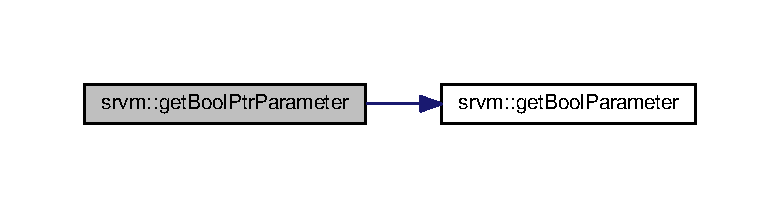
\includegraphics[width=350pt]{namespacesrvm_a4a300ace21cdfc4e753d7bbf97620f69_cgraph}
\end{center}
\end{figure}


\hypertarget{namespacesrvm_a0ceb768d016b217ced8c3d0b2a520862}{\index{srvm@{srvm}!get\-Flag\-Value\-To\-Print@{get\-Flag\-Value\-To\-Print}}
\index{get\-Flag\-Value\-To\-Print@{get\-Flag\-Value\-To\-Print}!srvm@{srvm}}
\subsubsection[{get\-Flag\-Value\-To\-Print}]{\setlength{\rightskip}{0pt plus 5cm}string srvm\-::get\-Flag\-Value\-To\-Print (
\begin{DoxyParamCaption}
\item[{bool}]{flag}
\end{DoxyParamCaption}
)}}\label{namespacesrvm_a0ceb768d016b217ced8c3d0b2a520862}


Definition at line 191 of file srv\-\_\-manager.\-h.



Referenced by main().

\hypertarget{namespacesrvm_a2d37598ea68edd23c273e90b7f544e85}{\index{srvm@{srvm}!get\-Path\-Parameter@{get\-Path\-Parameter}}
\index{get\-Path\-Parameter@{get\-Path\-Parameter}!srvm@{srvm}}
\subsubsection[{get\-Path\-Parameter}]{\setlength{\rightskip}{0pt plus 5cm}string srvm\-::get\-Path\-Parameter (
\begin{DoxyParamCaption}
\item[{string}]{input, }
\item[{const string}]{default\-Value}
\end{DoxyParamCaption}
)}}\label{namespacesrvm_a2d37598ea68edd23c273e90b7f544e85}


Definition at line 149 of file srv\-\_\-manager.\-h.



References D\-E\-F\-A\-U\-L\-T\-\_\-\-S\-Y\-M\-B\-O\-L, and pcm\-::\-P\-C\-Manager\-::get\-Fomratted\-Data().



Referenced by get\-Path\-Ptr\-Parameter().



Here is the call graph for this function\-:
\nopagebreak
\begin{figure}[H]
\begin{center}
\leavevmode
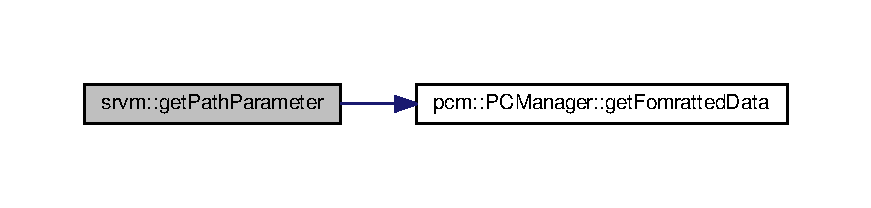
\includegraphics[width=350pt]{namespacesrvm_a2d37598ea68edd23c273e90b7f544e85_cgraph}
\end{center}
\end{figure}


\hypertarget{namespacesrvm_acad80730421eaf35cda6c8dcb0c3b4d6}{\index{srvm@{srvm}!get\-Path\-Ptr\-Parameter@{get\-Path\-Ptr\-Parameter}}
\index{get\-Path\-Ptr\-Parameter@{get\-Path\-Ptr\-Parameter}!srvm@{srvm}}
\subsubsection[{get\-Path\-Ptr\-Parameter}]{\setlength{\rightskip}{0pt plus 5cm}string srvm\-::get\-Path\-Ptr\-Parameter (
\begin{DoxyParamCaption}
\item[{char $\ast$}]{input, }
\item[{const string}]{default\-Value}
\end{DoxyParamCaption}
)}}\label{namespacesrvm_acad80730421eaf35cda6c8dcb0c3b4d6}


Definition at line 158 of file srv\-\_\-manager.\-h.



References get\-Path\-Parameter().



Referenced by main().



Here is the call graph for this function\-:
\nopagebreak
\begin{figure}[H]
\begin{center}
\leavevmode
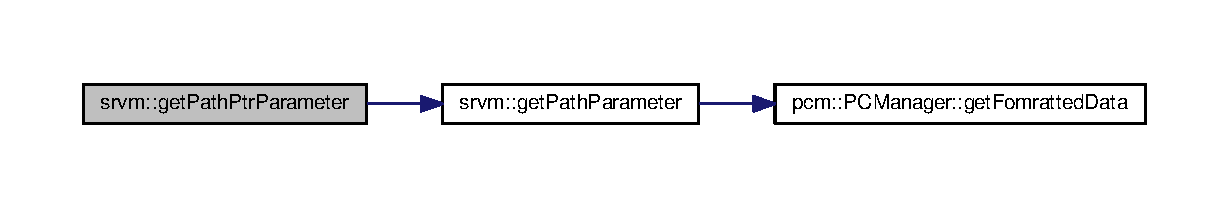
\includegraphics[width=350pt]{namespacesrvm_acad80730421eaf35cda6c8dcb0c3b4d6_cgraph}
\end{center}
\end{figure}


\hypertarget{namespacesrvm_a40e6c519b06c6f44c4706e35ccd2b3dd}{\index{srvm@{srvm}!get\-Service3\-D\-Array\-Parameter@{get\-Service3\-D\-Array\-Parameter}}
\index{get\-Service3\-D\-Array\-Parameter@{get\-Service3\-D\-Array\-Parameter}!srvm@{srvm}}
\subsubsection[{get\-Service3\-D\-Array\-Parameter}]{\setlength{\rightskip}{0pt plus 5cm}vector$<$float$>$ srvm\-::get\-Service3\-D\-Array\-Parameter (
\begin{DoxyParamCaption}
\item[{vector$<$ float $>$}]{input, }
\item[{const vector$<$ float $>$}]{default\-Value}
\end{DoxyParamCaption}
)}}\label{namespacesrvm_a40e6c519b06c6f44c4706e35ccd2b3dd}


Definition at line 176 of file srv\-\_\-manager.\-h.



Referenced by filter(), and initialize\-Input\-Parameters().

\hypertarget{namespacesrvm_a6fcb13a6186c7beda4a120b1a4f46313}{\index{srvm@{srvm}!get\-Service3\-D\-Array\-Parameter@{get\-Service3\-D\-Array\-Parameter}}
\index{get\-Service3\-D\-Array\-Parameter@{get\-Service3\-D\-Array\-Parameter}!srvm@{srvm}}
\subsubsection[{get\-Service3\-D\-Array\-Parameter}]{\setlength{\rightskip}{0pt plus 5cm}vector$<$float$>$ srvm\-::get\-Service3\-D\-Array\-Parameter (
\begin{DoxyParamCaption}
\item[{vector$<$ float $>$}]{input, }
\item[{const float}]{default\-Value\mbox{[}$\,$\mbox{]}}
\end{DoxyParamCaption}
)}}\label{namespacesrvm_a6fcb13a6186c7beda4a120b1a4f46313}


Definition at line 185 of file srv\-\_\-manager.\-h.



References get3\-D\-Array().



Here is the call graph for this function\-:
\nopagebreak
\begin{figure}[H]
\begin{center}
\leavevmode
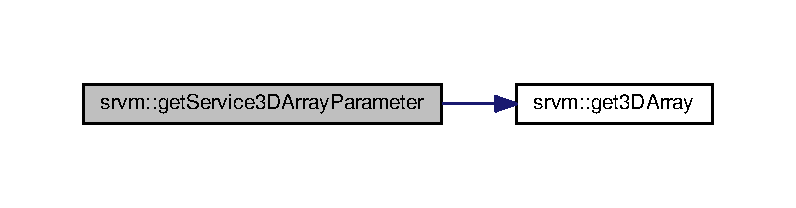
\includegraphics[width=350pt]{namespacesrvm_a6fcb13a6186c7beda4a120b1a4f46313_cgraph}
\end{center}
\end{figure}


\hypertarget{namespacesrvm_ab17b035d854cf06a49bf869d1c23d76d}{\index{srvm@{srvm}!get\-Service\-Float\-Parameter@{get\-Service\-Float\-Parameter}}
\index{get\-Service\-Float\-Parameter@{get\-Service\-Float\-Parameter}!srvm@{srvm}}
\subsubsection[{get\-Service\-Float\-Parameter}]{\setlength{\rightskip}{0pt plus 5cm}float srvm\-::get\-Service\-Float\-Parameter (
\begin{DoxyParamCaption}
\item[{float}]{input, }
\item[{const float}]{default\-Value}
\end{DoxyParamCaption}
)}}\label{namespacesrvm_ab17b035d854cf06a49bf869d1c23d76d}


Definition at line 163 of file srv\-\_\-manager.\-h.



Referenced by deep\-Filtering(), and initialize\-Input\-Parameters().

\hypertarget{namespacesrvm_aca4253032e76670dd7e7b3c31fb59714}{\index{srvm@{srvm}!get\-Service\-Int\-Parameter@{get\-Service\-Int\-Parameter}}
\index{get\-Service\-Int\-Parameter@{get\-Service\-Int\-Parameter}!srvm@{srvm}}
\subsubsection[{get\-Service\-Int\-Parameter}]{\setlength{\rightskip}{0pt plus 5cm}int srvm\-::get\-Service\-Int\-Parameter (
\begin{DoxyParamCaption}
\item[{int}]{input, }
\item[{const int}]{default\-Value}
\end{DoxyParamCaption}
)}}\label{namespacesrvm_aca4253032e76670dd7e7b3c31fb59714}


Definition at line 168 of file srv\-\_\-manager.\-h.



Referenced by initialize\-Input\-Parameters().

\hypertarget{namespacesrvm_a26454c4e5c30136db86cb0aa0f5a91b0}{\index{srvm@{srvm}!get\-Service\-String\-Parameter@{get\-Service\-String\-Parameter}}
\index{get\-Service\-String\-Parameter@{get\-Service\-String\-Parameter}!srvm@{srvm}}
\subsubsection[{get\-Service\-String\-Parameter}]{\setlength{\rightskip}{0pt plus 5cm}string srvm\-::get\-Service\-String\-Parameter (
\begin{DoxyParamCaption}
\item[{string}]{input, }
\item[{const string}]{default\-Value}
\end{DoxyParamCaption}
)}}\label{namespacesrvm_a26454c4e5c30136db86cb0aa0f5a91b0}


Definition at line 173 of file srv\-\_\-manager.\-h.



References get\-String\-Parameter().



Here is the call graph for this function\-:
\nopagebreak
\begin{figure}[H]
\begin{center}
\leavevmode
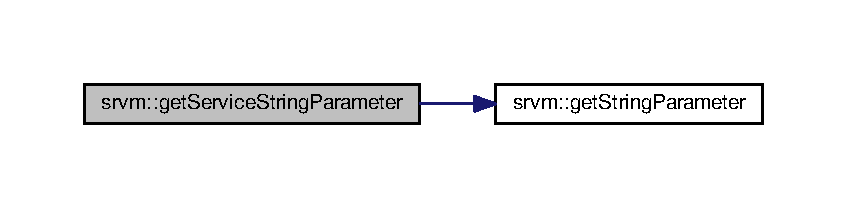
\includegraphics[width=350pt]{namespacesrvm_a26454c4e5c30136db86cb0aa0f5a91b0_cgraph}
\end{center}
\end{figure}


\hypertarget{namespacesrvm_a9c76ccfdb20b5ade1a837f4888a64997}{\index{srvm@{srvm}!get\-String\-Parameter@{get\-String\-Parameter}}
\index{get\-String\-Parameter@{get\-String\-Parameter}!srvm@{srvm}}
\subsubsection[{get\-String\-Parameter}]{\setlength{\rightskip}{0pt plus 5cm}string srvm\-::get\-String\-Parameter (
\begin{DoxyParamCaption}
\item[{string}]{input, }
\item[{const string}]{default\-Value}
\end{DoxyParamCaption}
)}}\label{namespacesrvm_a9c76ccfdb20b5ade1a837f4888a64997}


Definition at line 129 of file srv\-\_\-manager.\-h.



References D\-E\-F\-A\-U\-L\-T\-\_\-\-S\-Y\-M\-B\-O\-L.



Referenced by get\-Service\-String\-Parameter(), get\-String\-Ptr\-Parameter(), and main().

\hypertarget{namespacesrvm_a2fe9c141c7827eaa0269319f179dfee5}{\index{srvm@{srvm}!get\-String\-Ptr\-Parameter@{get\-String\-Ptr\-Parameter}}
\index{get\-String\-Ptr\-Parameter@{get\-String\-Ptr\-Parameter}!srvm@{srvm}}
\subsubsection[{get\-String\-Ptr\-Parameter}]{\setlength{\rightskip}{0pt plus 5cm}string srvm\-::get\-String\-Ptr\-Parameter (
\begin{DoxyParamCaption}
\item[{char $\ast$}]{input, }
\item[{const string}]{default\-Value}
\end{DoxyParamCaption}
)}}\label{namespacesrvm_a2fe9c141c7827eaa0269319f179dfee5}


Definition at line 134 of file srv\-\_\-manager.\-h.



References get\-String\-Parameter().



Referenced by main().



Here is the call graph for this function\-:
\nopagebreak
\begin{figure}[H]
\begin{center}
\leavevmode
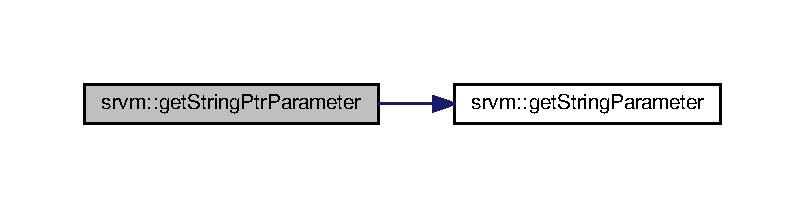
\includegraphics[width=350pt]{namespacesrvm_a2fe9c141c7827eaa0269319f179dfee5_cgraph}
\end{center}
\end{figure}




\subsection{Variable Documentation}
\hypertarget{namespacesrvm_a92921b8b79655fa69a697a54dca42056}{\index{srvm@{srvm}!D\-E\-F\-A\-U\-L\-T\-\_\-\-I\-N\-P\-U\-T\-\_\-\-P\-A\-R\-A\-M\-\_\-\-C\-E\-N\-T\-R\-O\-I\-D\-\_\-\-L\-O\-G\-\_\-\-F\-I\-L\-E@{D\-E\-F\-A\-U\-L\-T\-\_\-\-I\-N\-P\-U\-T\-\_\-\-P\-A\-R\-A\-M\-\_\-\-C\-E\-N\-T\-R\-O\-I\-D\-\_\-\-L\-O\-G\-\_\-\-F\-I\-L\-E}}
\index{D\-E\-F\-A\-U\-L\-T\-\_\-\-I\-N\-P\-U\-T\-\_\-\-P\-A\-R\-A\-M\-\_\-\-C\-E\-N\-T\-R\-O\-I\-D\-\_\-\-L\-O\-G\-\_\-\-F\-I\-L\-E@{D\-E\-F\-A\-U\-L\-T\-\_\-\-I\-N\-P\-U\-T\-\_\-\-P\-A\-R\-A\-M\-\_\-\-C\-E\-N\-T\-R\-O\-I\-D\-\_\-\-L\-O\-G\-\_\-\-F\-I\-L\-E}!srvm@{srvm}}
\subsubsection[{D\-E\-F\-A\-U\-L\-T\-\_\-\-I\-N\-P\-U\-T\-\_\-\-P\-A\-R\-A\-M\-\_\-\-C\-E\-N\-T\-R\-O\-I\-D\-\_\-\-L\-O\-G\-\_\-\-F\-I\-L\-E}]{\setlength{\rightskip}{0pt plus 5cm}const string srvm\-::\-D\-E\-F\-A\-U\-L\-T\-\_\-\-I\-N\-P\-U\-T\-\_\-\-P\-A\-R\-A\-M\-\_\-\-C\-E\-N\-T\-R\-O\-I\-D\-\_\-\-L\-O\-G\-\_\-\-F\-I\-L\-E = \char`\"{}\char`\"{}}}\label{namespacesrvm_a92921b8b79655fa69a697a54dca42056}


Definition at line 101 of file srv\-\_\-manager.\-h.



Referenced by main().

\hypertarget{namespacesrvm_afb9bab9dced618a8992cf505cf484b1c}{\index{srvm@{srvm}!D\-E\-F\-A\-U\-L\-T\-\_\-\-I\-N\-P\-U\-T\-\_\-\-P\-A\-R\-A\-M\-\_\-\-R\-A\-W\-\_\-\-C\-L\-O\-U\-D\-\_\-\-T\-O\-P\-I\-C@{D\-E\-F\-A\-U\-L\-T\-\_\-\-I\-N\-P\-U\-T\-\_\-\-P\-A\-R\-A\-M\-\_\-\-R\-A\-W\-\_\-\-C\-L\-O\-U\-D\-\_\-\-T\-O\-P\-I\-C}}
\index{D\-E\-F\-A\-U\-L\-T\-\_\-\-I\-N\-P\-U\-T\-\_\-\-P\-A\-R\-A\-M\-\_\-\-R\-A\-W\-\_\-\-C\-L\-O\-U\-D\-\_\-\-T\-O\-P\-I\-C@{D\-E\-F\-A\-U\-L\-T\-\_\-\-I\-N\-P\-U\-T\-\_\-\-P\-A\-R\-A\-M\-\_\-\-R\-A\-W\-\_\-\-C\-L\-O\-U\-D\-\_\-\-T\-O\-P\-I\-C}!srvm@{srvm}}
\subsubsection[{D\-E\-F\-A\-U\-L\-T\-\_\-\-I\-N\-P\-U\-T\-\_\-\-P\-A\-R\-A\-M\-\_\-\-R\-A\-W\-\_\-\-C\-L\-O\-U\-D\-\_\-\-T\-O\-P\-I\-C}]{\setlength{\rightskip}{0pt plus 5cm}const string srvm\-::\-D\-E\-F\-A\-U\-L\-T\-\_\-\-I\-N\-P\-U\-T\-\_\-\-P\-A\-R\-A\-M\-\_\-\-R\-A\-W\-\_\-\-C\-L\-O\-U\-D\-\_\-\-T\-O\-P\-I\-C = \char`\"{}/camera/depth/points\char`\"{}}}\label{namespacesrvm_afb9bab9dced618a8992cf505cf484b1c}


Definition at line 100 of file srv\-\_\-manager.\-h.



Referenced by main().

\hypertarget{namespacesrvm_aef053199a3f95b1da712ef187b096f93}{\index{srvm@{srvm}!D\-E\-F\-A\-U\-L\-T\-\_\-\-I\-N\-P\-U\-T\-\_\-\-P\-A\-R\-A\-M\-\_\-\-S\-H\-O\-W\-\_\-\-C\-L\-U\-S\-T\-E\-R\-S@{D\-E\-F\-A\-U\-L\-T\-\_\-\-I\-N\-P\-U\-T\-\_\-\-P\-A\-R\-A\-M\-\_\-\-S\-H\-O\-W\-\_\-\-C\-L\-U\-S\-T\-E\-R\-S}}
\index{D\-E\-F\-A\-U\-L\-T\-\_\-\-I\-N\-P\-U\-T\-\_\-\-P\-A\-R\-A\-M\-\_\-\-S\-H\-O\-W\-\_\-\-C\-L\-U\-S\-T\-E\-R\-S@{D\-E\-F\-A\-U\-L\-T\-\_\-\-I\-N\-P\-U\-T\-\_\-\-P\-A\-R\-A\-M\-\_\-\-S\-H\-O\-W\-\_\-\-C\-L\-U\-S\-T\-E\-R\-S}!srvm@{srvm}}
\subsubsection[{D\-E\-F\-A\-U\-L\-T\-\_\-\-I\-N\-P\-U\-T\-\_\-\-P\-A\-R\-A\-M\-\_\-\-S\-H\-O\-W\-\_\-\-C\-L\-U\-S\-T\-E\-R\-S}]{\setlength{\rightskip}{0pt plus 5cm}const bool srvm\-::\-D\-E\-F\-A\-U\-L\-T\-\_\-\-I\-N\-P\-U\-T\-\_\-\-P\-A\-R\-A\-M\-\_\-\-S\-H\-O\-W\-\_\-\-C\-L\-U\-S\-T\-E\-R\-S = false}}\label{namespacesrvm_aef053199a3f95b1da712ef187b096f93}


Definition at line 105 of file srv\-\_\-manager.\-h.



Referenced by main().

\hypertarget{namespacesrvm_a8e6760e3e9557fc2fb87cbb6fcd8b3e6}{\index{srvm@{srvm}!D\-E\-F\-A\-U\-L\-T\-\_\-\-I\-N\-P\-U\-T\-\_\-\-P\-A\-R\-A\-M\-\_\-\-S\-H\-O\-W\-\_\-\-O\-B\-J\-E\-C\-T\-\_\-\-O\-N\-\_\-\-S\-U\-P\-P\-O\-R\-T@{D\-E\-F\-A\-U\-L\-T\-\_\-\-I\-N\-P\-U\-T\-\_\-\-P\-A\-R\-A\-M\-\_\-\-S\-H\-O\-W\-\_\-\-O\-B\-J\-E\-C\-T\-\_\-\-O\-N\-\_\-\-S\-U\-P\-P\-O\-R\-T}}
\index{D\-E\-F\-A\-U\-L\-T\-\_\-\-I\-N\-P\-U\-T\-\_\-\-P\-A\-R\-A\-M\-\_\-\-S\-H\-O\-W\-\_\-\-O\-B\-J\-E\-C\-T\-\_\-\-O\-N\-\_\-\-S\-U\-P\-P\-O\-R\-T@{D\-E\-F\-A\-U\-L\-T\-\_\-\-I\-N\-P\-U\-T\-\_\-\-P\-A\-R\-A\-M\-\_\-\-S\-H\-O\-W\-\_\-\-O\-B\-J\-E\-C\-T\-\_\-\-O\-N\-\_\-\-S\-U\-P\-P\-O\-R\-T}!srvm@{srvm}}
\subsubsection[{D\-E\-F\-A\-U\-L\-T\-\_\-\-I\-N\-P\-U\-T\-\_\-\-P\-A\-R\-A\-M\-\_\-\-S\-H\-O\-W\-\_\-\-O\-B\-J\-E\-C\-T\-\_\-\-O\-N\-\_\-\-S\-U\-P\-P\-O\-R\-T}]{\setlength{\rightskip}{0pt plus 5cm}const bool srvm\-::\-D\-E\-F\-A\-U\-L\-T\-\_\-\-I\-N\-P\-U\-T\-\_\-\-P\-A\-R\-A\-M\-\_\-\-S\-H\-O\-W\-\_\-\-O\-B\-J\-E\-C\-T\-\_\-\-O\-N\-\_\-\-S\-U\-P\-P\-O\-R\-T = false}}\label{namespacesrvm_a8e6760e3e9557fc2fb87cbb6fcd8b3e6}


Definition at line 104 of file srv\-\_\-manager.\-h.



Referenced by main().

\hypertarget{namespacesrvm_ac54afc31491c977345ef1a1fbb563be3}{\index{srvm@{srvm}!D\-E\-F\-A\-U\-L\-T\-\_\-\-I\-N\-P\-U\-T\-\_\-\-P\-A\-R\-A\-M\-\_\-\-S\-H\-O\-W\-\_\-\-O\-R\-I\-G\-I\-N\-A\-L\-\_\-\-C\-L\-O\-U\-D@{D\-E\-F\-A\-U\-L\-T\-\_\-\-I\-N\-P\-U\-T\-\_\-\-P\-A\-R\-A\-M\-\_\-\-S\-H\-O\-W\-\_\-\-O\-R\-I\-G\-I\-N\-A\-L\-\_\-\-C\-L\-O\-U\-D}}
\index{D\-E\-F\-A\-U\-L\-T\-\_\-\-I\-N\-P\-U\-T\-\_\-\-P\-A\-R\-A\-M\-\_\-\-S\-H\-O\-W\-\_\-\-O\-R\-I\-G\-I\-N\-A\-L\-\_\-\-C\-L\-O\-U\-D@{D\-E\-F\-A\-U\-L\-T\-\_\-\-I\-N\-P\-U\-T\-\_\-\-P\-A\-R\-A\-M\-\_\-\-S\-H\-O\-W\-\_\-\-O\-R\-I\-G\-I\-N\-A\-L\-\_\-\-C\-L\-O\-U\-D}!srvm@{srvm}}
\subsubsection[{D\-E\-F\-A\-U\-L\-T\-\_\-\-I\-N\-P\-U\-T\-\_\-\-P\-A\-R\-A\-M\-\_\-\-S\-H\-O\-W\-\_\-\-O\-R\-I\-G\-I\-N\-A\-L\-\_\-\-C\-L\-O\-U\-D}]{\setlength{\rightskip}{0pt plus 5cm}const bool srvm\-::\-D\-E\-F\-A\-U\-L\-T\-\_\-\-I\-N\-P\-U\-T\-\_\-\-P\-A\-R\-A\-M\-\_\-\-S\-H\-O\-W\-\_\-\-O\-R\-I\-G\-I\-N\-A\-L\-\_\-\-C\-L\-O\-U\-D = false}}\label{namespacesrvm_ac54afc31491c977345ef1a1fbb563be3}


Definition at line 102 of file srv\-\_\-manager.\-h.



Referenced by main().

\hypertarget{namespacesrvm_a9880144ef0df953c3b583e4f20dbff76}{\index{srvm@{srvm}!D\-E\-F\-A\-U\-L\-T\-\_\-\-I\-N\-P\-U\-T\-\_\-\-P\-A\-R\-A\-M\-\_\-\-S\-H\-O\-W\-\_\-\-S\-U\-P\-P\-O\-R\-T\-S@{D\-E\-F\-A\-U\-L\-T\-\_\-\-I\-N\-P\-U\-T\-\_\-\-P\-A\-R\-A\-M\-\_\-\-S\-H\-O\-W\-\_\-\-S\-U\-P\-P\-O\-R\-T\-S}}
\index{D\-E\-F\-A\-U\-L\-T\-\_\-\-I\-N\-P\-U\-T\-\_\-\-P\-A\-R\-A\-M\-\_\-\-S\-H\-O\-W\-\_\-\-S\-U\-P\-P\-O\-R\-T\-S@{D\-E\-F\-A\-U\-L\-T\-\_\-\-I\-N\-P\-U\-T\-\_\-\-P\-A\-R\-A\-M\-\_\-\-S\-H\-O\-W\-\_\-\-S\-U\-P\-P\-O\-R\-T\-S}!srvm@{srvm}}
\subsubsection[{D\-E\-F\-A\-U\-L\-T\-\_\-\-I\-N\-P\-U\-T\-\_\-\-P\-A\-R\-A\-M\-\_\-\-S\-H\-O\-W\-\_\-\-S\-U\-P\-P\-O\-R\-T\-S}]{\setlength{\rightskip}{0pt plus 5cm}const bool srvm\-::\-D\-E\-F\-A\-U\-L\-T\-\_\-\-I\-N\-P\-U\-T\-\_\-\-P\-A\-R\-A\-M\-\_\-\-S\-H\-O\-W\-\_\-\-S\-U\-P\-P\-O\-R\-T\-S = false}}\label{namespacesrvm_a9880144ef0df953c3b583e4f20dbff76}


Definition at line 103 of file srv\-\_\-manager.\-h.



Referenced by main().

\hypertarget{namespacesrvm_a9ae9e53a20ec9335fe07c1a42520198e}{\index{srvm@{srvm}!D\-E\-F\-A\-U\-L\-T\-\_\-\-P\-A\-R\-A\-M\-\_\-\-A\-R\-M\-\_\-\-S\-R\-V\-\_\-\-C\-A\-M\-E\-R\-A\-\_\-\-F\-R\-A\-M\-E@{D\-E\-F\-A\-U\-L\-T\-\_\-\-P\-A\-R\-A\-M\-\_\-\-A\-R\-M\-\_\-\-S\-R\-V\-\_\-\-C\-A\-M\-E\-R\-A\-\_\-\-F\-R\-A\-M\-E}}
\index{D\-E\-F\-A\-U\-L\-T\-\_\-\-P\-A\-R\-A\-M\-\_\-\-A\-R\-M\-\_\-\-S\-R\-V\-\_\-\-C\-A\-M\-E\-R\-A\-\_\-\-F\-R\-A\-M\-E@{D\-E\-F\-A\-U\-L\-T\-\_\-\-P\-A\-R\-A\-M\-\_\-\-A\-R\-M\-\_\-\-S\-R\-V\-\_\-\-C\-A\-M\-E\-R\-A\-\_\-\-F\-R\-A\-M\-E}!srvm@{srvm}}
\subsubsection[{D\-E\-F\-A\-U\-L\-T\-\_\-\-P\-A\-R\-A\-M\-\_\-\-A\-R\-M\-\_\-\-S\-R\-V\-\_\-\-C\-A\-M\-E\-R\-A\-\_\-\-F\-R\-A\-M\-E}]{\setlength{\rightskip}{0pt plus 5cm}const string srvm\-::\-D\-E\-F\-A\-U\-L\-T\-\_\-\-P\-A\-R\-A\-M\-\_\-\-A\-R\-M\-\_\-\-S\-R\-V\-\_\-\-C\-A\-M\-E\-R\-A\-\_\-\-F\-R\-A\-M\-E = \char`\"{}/camera\-\_\-depth\-\_\-optical\-\_\-frame\char`\"{}}}\label{namespacesrvm_a9ae9e53a20ec9335fe07c1a42520198e}


Definition at line 106 of file srv\-\_\-manager.\-h.



Referenced by main().

\hypertarget{namespacesrvm_ab8271bafa5b004c13196b24b77cef53a}{\index{srvm@{srvm}!D\-E\-F\-A\-U\-L\-T\-\_\-\-P\-A\-R\-A\-M\-\_\-\-A\-R\-M\-\_\-\-S\-R\-V\-\_\-\-L\-E\-F\-T\-\_\-\-E\-L\-B\-O\-W\-\_\-\-F\-R\-A\-M\-E@{D\-E\-F\-A\-U\-L\-T\-\_\-\-P\-A\-R\-A\-M\-\_\-\-A\-R\-M\-\_\-\-S\-R\-V\-\_\-\-L\-E\-F\-T\-\_\-\-E\-L\-B\-O\-W\-\_\-\-F\-R\-A\-M\-E}}
\index{D\-E\-F\-A\-U\-L\-T\-\_\-\-P\-A\-R\-A\-M\-\_\-\-A\-R\-M\-\_\-\-S\-R\-V\-\_\-\-L\-E\-F\-T\-\_\-\-E\-L\-B\-O\-W\-\_\-\-F\-R\-A\-M\-E@{D\-E\-F\-A\-U\-L\-T\-\_\-\-P\-A\-R\-A\-M\-\_\-\-A\-R\-M\-\_\-\-S\-R\-V\-\_\-\-L\-E\-F\-T\-\_\-\-E\-L\-B\-O\-W\-\_\-\-F\-R\-A\-M\-E}!srvm@{srvm}}
\subsubsection[{D\-E\-F\-A\-U\-L\-T\-\_\-\-P\-A\-R\-A\-M\-\_\-\-A\-R\-M\-\_\-\-S\-R\-V\-\_\-\-L\-E\-F\-T\-\_\-\-E\-L\-B\-O\-W\-\_\-\-F\-R\-A\-M\-E}]{\setlength{\rightskip}{0pt plus 5cm}const string srvm\-::\-D\-E\-F\-A\-U\-L\-T\-\_\-\-P\-A\-R\-A\-M\-\_\-\-A\-R\-M\-\_\-\-S\-R\-V\-\_\-\-L\-E\-F\-T\-\_\-\-E\-L\-B\-O\-W\-\_\-\-F\-R\-A\-M\-E = \char`\"{}/left\-\_\-lower\-\_\-elbow\char`\"{}}}\label{namespacesrvm_ab8271bafa5b004c13196b24b77cef53a}


Definition at line 110 of file srv\-\_\-manager.\-h.



Referenced by main().

\hypertarget{namespacesrvm_af63966bf248ec14ccf2a2ca74fa1214d}{\index{srvm@{srvm}!D\-E\-F\-A\-U\-L\-T\-\_\-\-P\-A\-R\-A\-M\-\_\-\-A\-R\-M\-\_\-\-S\-R\-V\-\_\-\-L\-E\-F\-T\-\_\-\-F\-O\-R\-E\-A\-R\-M\-\_\-\-F\-R\-A\-M\-E@{D\-E\-F\-A\-U\-L\-T\-\_\-\-P\-A\-R\-A\-M\-\_\-\-A\-R\-M\-\_\-\-S\-R\-V\-\_\-\-L\-E\-F\-T\-\_\-\-F\-O\-R\-E\-A\-R\-M\-\_\-\-F\-R\-A\-M\-E}}
\index{D\-E\-F\-A\-U\-L\-T\-\_\-\-P\-A\-R\-A\-M\-\_\-\-A\-R\-M\-\_\-\-S\-R\-V\-\_\-\-L\-E\-F\-T\-\_\-\-F\-O\-R\-E\-A\-R\-M\-\_\-\-F\-R\-A\-M\-E@{D\-E\-F\-A\-U\-L\-T\-\_\-\-P\-A\-R\-A\-M\-\_\-\-A\-R\-M\-\_\-\-S\-R\-V\-\_\-\-L\-E\-F\-T\-\_\-\-F\-O\-R\-E\-A\-R\-M\-\_\-\-F\-R\-A\-M\-E}!srvm@{srvm}}
\subsubsection[{D\-E\-F\-A\-U\-L\-T\-\_\-\-P\-A\-R\-A\-M\-\_\-\-A\-R\-M\-\_\-\-S\-R\-V\-\_\-\-L\-E\-F\-T\-\_\-\-F\-O\-R\-E\-A\-R\-M\-\_\-\-F\-R\-A\-M\-E}]{\setlength{\rightskip}{0pt plus 5cm}const string srvm\-::\-D\-E\-F\-A\-U\-L\-T\-\_\-\-P\-A\-R\-A\-M\-\_\-\-A\-R\-M\-\_\-\-S\-R\-V\-\_\-\-L\-E\-F\-T\-\_\-\-F\-O\-R\-E\-A\-R\-M\-\_\-\-F\-R\-A\-M\-E = \char`\"{}/left\-\_\-lower\-\_\-forearm\char`\"{}}}\label{namespacesrvm_af63966bf248ec14ccf2a2ca74fa1214d}


Definition at line 108 of file srv\-\_\-manager.\-h.



Referenced by main().

\hypertarget{namespacesrvm_acb12c9f4a5661db79a05ea222c83e215}{\index{srvm@{srvm}!D\-E\-F\-A\-U\-L\-T\-\_\-\-P\-A\-R\-A\-M\-\_\-\-A\-R\-M\-\_\-\-S\-R\-V\-\_\-\-R\-I\-G\-H\-T\-\_\-\-E\-L\-B\-O\-W\-\_\-\-F\-R\-A\-M\-E@{D\-E\-F\-A\-U\-L\-T\-\_\-\-P\-A\-R\-A\-M\-\_\-\-A\-R\-M\-\_\-\-S\-R\-V\-\_\-\-R\-I\-G\-H\-T\-\_\-\-E\-L\-B\-O\-W\-\_\-\-F\-R\-A\-M\-E}}
\index{D\-E\-F\-A\-U\-L\-T\-\_\-\-P\-A\-R\-A\-M\-\_\-\-A\-R\-M\-\_\-\-S\-R\-V\-\_\-\-R\-I\-G\-H\-T\-\_\-\-E\-L\-B\-O\-W\-\_\-\-F\-R\-A\-M\-E@{D\-E\-F\-A\-U\-L\-T\-\_\-\-P\-A\-R\-A\-M\-\_\-\-A\-R\-M\-\_\-\-S\-R\-V\-\_\-\-R\-I\-G\-H\-T\-\_\-\-E\-L\-B\-O\-W\-\_\-\-F\-R\-A\-M\-E}!srvm@{srvm}}
\subsubsection[{D\-E\-F\-A\-U\-L\-T\-\_\-\-P\-A\-R\-A\-M\-\_\-\-A\-R\-M\-\_\-\-S\-R\-V\-\_\-\-R\-I\-G\-H\-T\-\_\-\-E\-L\-B\-O\-W\-\_\-\-F\-R\-A\-M\-E}]{\setlength{\rightskip}{0pt plus 5cm}const string srvm\-::\-D\-E\-F\-A\-U\-L\-T\-\_\-\-P\-A\-R\-A\-M\-\_\-\-A\-R\-M\-\_\-\-S\-R\-V\-\_\-\-R\-I\-G\-H\-T\-\_\-\-E\-L\-B\-O\-W\-\_\-\-F\-R\-A\-M\-E = \char`\"{}/right\-\_\-lower\-\_\-elbow\char`\"{}}}\label{namespacesrvm_acb12c9f4a5661db79a05ea222c83e215}


Definition at line 109 of file srv\-\_\-manager.\-h.



Referenced by main().

\hypertarget{namespacesrvm_a6e203b3aafd97558c58ada022c9cc514}{\index{srvm@{srvm}!D\-E\-F\-A\-U\-L\-T\-\_\-\-P\-A\-R\-A\-M\-\_\-\-A\-R\-M\-\_\-\-S\-R\-V\-\_\-\-R\-I\-G\-H\-T\-\_\-\-F\-O\-R\-E\-A\-R\-M\-\_\-\-F\-R\-A\-M\-E@{D\-E\-F\-A\-U\-L\-T\-\_\-\-P\-A\-R\-A\-M\-\_\-\-A\-R\-M\-\_\-\-S\-R\-V\-\_\-\-R\-I\-G\-H\-T\-\_\-\-F\-O\-R\-E\-A\-R\-M\-\_\-\-F\-R\-A\-M\-E}}
\index{D\-E\-F\-A\-U\-L\-T\-\_\-\-P\-A\-R\-A\-M\-\_\-\-A\-R\-M\-\_\-\-S\-R\-V\-\_\-\-R\-I\-G\-H\-T\-\_\-\-F\-O\-R\-E\-A\-R\-M\-\_\-\-F\-R\-A\-M\-E@{D\-E\-F\-A\-U\-L\-T\-\_\-\-P\-A\-R\-A\-M\-\_\-\-A\-R\-M\-\_\-\-S\-R\-V\-\_\-\-R\-I\-G\-H\-T\-\_\-\-F\-O\-R\-E\-A\-R\-M\-\_\-\-F\-R\-A\-M\-E}!srvm@{srvm}}
\subsubsection[{D\-E\-F\-A\-U\-L\-T\-\_\-\-P\-A\-R\-A\-M\-\_\-\-A\-R\-M\-\_\-\-S\-R\-V\-\_\-\-R\-I\-G\-H\-T\-\_\-\-F\-O\-R\-E\-A\-R\-M\-\_\-\-F\-R\-A\-M\-E}]{\setlength{\rightskip}{0pt plus 5cm}const string srvm\-::\-D\-E\-F\-A\-U\-L\-T\-\_\-\-P\-A\-R\-A\-M\-\_\-\-A\-R\-M\-\_\-\-S\-R\-V\-\_\-\-R\-I\-G\-H\-T\-\_\-\-F\-O\-R\-E\-A\-R\-M\-\_\-\-F\-R\-A\-M\-E = \char`\"{}/right\-\_\-lower\-\_\-forearm\char`\"{}}}\label{namespacesrvm_a6e203b3aafd97558c58ada022c9cc514}


Definition at line 107 of file srv\-\_\-manager.\-h.



Referenced by main().

\hypertarget{namespacesrvm_a7fdc748a5c9f8f7211d6e32e64f96c63}{\index{srvm@{srvm}!D\-E\-F\-A\-U\-L\-T\-\_\-\-P\-A\-R\-A\-M\-\_\-\-A\-R\-M\-\_\-\-S\-R\-V\-\_\-\-S\-H\-O\-W\-\_\-\-C\-L\-O\-U\-D\-S@{D\-E\-F\-A\-U\-L\-T\-\_\-\-P\-A\-R\-A\-M\-\_\-\-A\-R\-M\-\_\-\-S\-R\-V\-\_\-\-S\-H\-O\-W\-\_\-\-C\-L\-O\-U\-D\-S}}
\index{D\-E\-F\-A\-U\-L\-T\-\_\-\-P\-A\-R\-A\-M\-\_\-\-A\-R\-M\-\_\-\-S\-R\-V\-\_\-\-S\-H\-O\-W\-\_\-\-C\-L\-O\-U\-D\-S@{D\-E\-F\-A\-U\-L\-T\-\_\-\-P\-A\-R\-A\-M\-\_\-\-A\-R\-M\-\_\-\-S\-R\-V\-\_\-\-S\-H\-O\-W\-\_\-\-C\-L\-O\-U\-D\-S}!srvm@{srvm}}
\subsubsection[{D\-E\-F\-A\-U\-L\-T\-\_\-\-P\-A\-R\-A\-M\-\_\-\-A\-R\-M\-\_\-\-S\-R\-V\-\_\-\-S\-H\-O\-W\-\_\-\-C\-L\-O\-U\-D\-S}]{\setlength{\rightskip}{0pt plus 5cm}const bool srvm\-::\-D\-E\-F\-A\-U\-L\-T\-\_\-\-P\-A\-R\-A\-M\-\_\-\-A\-R\-M\-\_\-\-S\-R\-V\-\_\-\-S\-H\-O\-W\-\_\-\-C\-L\-O\-U\-D\-S = false}}\label{namespacesrvm_a7fdc748a5c9f8f7211d6e32e64f96c63}


Definition at line 111 of file srv\-\_\-manager.\-h.



Referenced by main().

\hypertarget{namespacesrvm_a2c4c31d893bfef55ede38ab56f4e7658}{\index{srvm@{srvm}!D\-E\-F\-A\-U\-L\-T\-\_\-\-P\-A\-R\-A\-M\-\_\-\-I\-N\-P\-U\-T\-\_\-\-C\-L\-O\-U\-D\-\_\-\-R\-E\-F\-E\-R\-E\-N\-C\-E\-\_\-\-F\-R\-A\-M\-E@{D\-E\-F\-A\-U\-L\-T\-\_\-\-P\-A\-R\-A\-M\-\_\-\-I\-N\-P\-U\-T\-\_\-\-C\-L\-O\-U\-D\-\_\-\-R\-E\-F\-E\-R\-E\-N\-C\-E\-\_\-\-F\-R\-A\-M\-E}}
\index{D\-E\-F\-A\-U\-L\-T\-\_\-\-P\-A\-R\-A\-M\-\_\-\-I\-N\-P\-U\-T\-\_\-\-C\-L\-O\-U\-D\-\_\-\-R\-E\-F\-E\-R\-E\-N\-C\-E\-\_\-\-F\-R\-A\-M\-E@{D\-E\-F\-A\-U\-L\-T\-\_\-\-P\-A\-R\-A\-M\-\_\-\-I\-N\-P\-U\-T\-\_\-\-C\-L\-O\-U\-D\-\_\-\-R\-E\-F\-E\-R\-E\-N\-C\-E\-\_\-\-F\-R\-A\-M\-E}!srvm@{srvm}}
\subsubsection[{D\-E\-F\-A\-U\-L\-T\-\_\-\-P\-A\-R\-A\-M\-\_\-\-I\-N\-P\-U\-T\-\_\-\-C\-L\-O\-U\-D\-\_\-\-R\-E\-F\-E\-R\-E\-N\-C\-E\-\_\-\-F\-R\-A\-M\-E}]{\setlength{\rightskip}{0pt plus 5cm}const string srvm\-::\-D\-E\-F\-A\-U\-L\-T\-\_\-\-P\-A\-R\-A\-M\-\_\-\-I\-N\-P\-U\-T\-\_\-\-C\-L\-O\-U\-D\-\_\-\-R\-E\-F\-E\-R\-E\-N\-C\-E\-\_\-\-F\-R\-A\-M\-E = \char`\"{}/camera\-\_\-depth\-\_\-optical\-\_\-frame\char`\"{}}}\label{namespacesrvm_a2c4c31d893bfef55ede38ab56f4e7658}


Definition at line 98 of file srv\-\_\-manager.\-h.



Referenced by main().

\hypertarget{namespacesrvm_a228565e6d2ec6f457f78c4412d6c7daa}{\index{srvm@{srvm}!D\-E\-F\-A\-U\-L\-T\-\_\-\-P\-A\-R\-A\-M\-\_\-\-O\-U\-T\-P\-U\-T\-\_\-\-C\-L\-O\-U\-D\-\_\-\-R\-E\-F\-E\-R\-E\-N\-C\-E\-\_\-\-F\-R\-A\-M\-E@{D\-E\-F\-A\-U\-L\-T\-\_\-\-P\-A\-R\-A\-M\-\_\-\-O\-U\-T\-P\-U\-T\-\_\-\-C\-L\-O\-U\-D\-\_\-\-R\-E\-F\-E\-R\-E\-N\-C\-E\-\_\-\-F\-R\-A\-M\-E}}
\index{D\-E\-F\-A\-U\-L\-T\-\_\-\-P\-A\-R\-A\-M\-\_\-\-O\-U\-T\-P\-U\-T\-\_\-\-C\-L\-O\-U\-D\-\_\-\-R\-E\-F\-E\-R\-E\-N\-C\-E\-\_\-\-F\-R\-A\-M\-E@{D\-E\-F\-A\-U\-L\-T\-\_\-\-P\-A\-R\-A\-M\-\_\-\-O\-U\-T\-P\-U\-T\-\_\-\-C\-L\-O\-U\-D\-\_\-\-R\-E\-F\-E\-R\-E\-N\-C\-E\-\_\-\-F\-R\-A\-M\-E}!srvm@{srvm}}
\subsubsection[{D\-E\-F\-A\-U\-L\-T\-\_\-\-P\-A\-R\-A\-M\-\_\-\-O\-U\-T\-P\-U\-T\-\_\-\-C\-L\-O\-U\-D\-\_\-\-R\-E\-F\-E\-R\-E\-N\-C\-E\-\_\-\-F\-R\-A\-M\-E}]{\setlength{\rightskip}{0pt plus 5cm}const string srvm\-::\-D\-E\-F\-A\-U\-L\-T\-\_\-\-P\-A\-R\-A\-M\-\_\-\-O\-U\-T\-P\-U\-T\-\_\-\-C\-L\-O\-U\-D\-\_\-\-R\-E\-F\-E\-R\-E\-N\-C\-E\-\_\-\-F\-R\-A\-M\-E = \char`\"{}/world\char`\"{}}}\label{namespacesrvm_a228565e6d2ec6f457f78c4412d6c7daa}


Definition at line 99 of file srv\-\_\-manager.\-h.



Referenced by main().

\hypertarget{namespacesrvm_a07324815e3638c6740336e50699d3300}{\index{srvm@{srvm}!D\-E\-F\-A\-U\-L\-T\-\_\-\-S\-E\-R\-V\-I\-C\-E\-\_\-\-A\-R\-R\-A\-Y\-\_\-\-P\-A\-R\-A\-M\-E\-T\-E\-R\-\_\-\-R\-E\-Q\-U\-E\-S\-T@{D\-E\-F\-A\-U\-L\-T\-\_\-\-S\-E\-R\-V\-I\-C\-E\-\_\-\-A\-R\-R\-A\-Y\-\_\-\-P\-A\-R\-A\-M\-E\-T\-E\-R\-\_\-\-R\-E\-Q\-U\-E\-S\-T}}
\index{D\-E\-F\-A\-U\-L\-T\-\_\-\-S\-E\-R\-V\-I\-C\-E\-\_\-\-A\-R\-R\-A\-Y\-\_\-\-P\-A\-R\-A\-M\-E\-T\-E\-R\-\_\-\-R\-E\-Q\-U\-E\-S\-T@{D\-E\-F\-A\-U\-L\-T\-\_\-\-S\-E\-R\-V\-I\-C\-E\-\_\-\-A\-R\-R\-A\-Y\-\_\-\-P\-A\-R\-A\-M\-E\-T\-E\-R\-\_\-\-R\-E\-Q\-U\-E\-S\-T}!srvm@{srvm}}
\subsubsection[{D\-E\-F\-A\-U\-L\-T\-\_\-\-S\-E\-R\-V\-I\-C\-E\-\_\-\-A\-R\-R\-A\-Y\-\_\-\-P\-A\-R\-A\-M\-E\-T\-E\-R\-\_\-\-R\-E\-Q\-U\-E\-S\-T}]{\setlength{\rightskip}{0pt plus 5cm}const float srvm\-::\-D\-E\-F\-A\-U\-L\-T\-\_\-\-S\-E\-R\-V\-I\-C\-E\-\_\-\-A\-R\-R\-A\-Y\-\_\-\-P\-A\-R\-A\-M\-E\-T\-E\-R\-\_\-\-R\-E\-Q\-U\-E\-S\-T\mbox{[}1\mbox{]} = \{-\/1\}}}\label{namespacesrvm_a07324815e3638c6740336e50699d3300}


Definition at line 120 of file srv\-\_\-manager.\-h.

\hypertarget{namespacesrvm_a27b2693a98ba8791767e3c8bebdab105}{\index{srvm@{srvm}!D\-E\-F\-A\-U\-L\-T\-\_\-\-S\-E\-R\-V\-I\-C\-E\-\_\-\-P\-A\-R\-A\-M\-E\-T\-E\-R\-\_\-\-R\-E\-Q\-U\-E\-S\-T@{D\-E\-F\-A\-U\-L\-T\-\_\-\-S\-E\-R\-V\-I\-C\-E\-\_\-\-P\-A\-R\-A\-M\-E\-T\-E\-R\-\_\-\-R\-E\-Q\-U\-E\-S\-T}}
\index{D\-E\-F\-A\-U\-L\-T\-\_\-\-S\-E\-R\-V\-I\-C\-E\-\_\-\-P\-A\-R\-A\-M\-E\-T\-E\-R\-\_\-\-R\-E\-Q\-U\-E\-S\-T@{D\-E\-F\-A\-U\-L\-T\-\_\-\-S\-E\-R\-V\-I\-C\-E\-\_\-\-P\-A\-R\-A\-M\-E\-T\-E\-R\-\_\-\-R\-E\-Q\-U\-E\-S\-T}!srvm@{srvm}}
\subsubsection[{D\-E\-F\-A\-U\-L\-T\-\_\-\-S\-E\-R\-V\-I\-C\-E\-\_\-\-P\-A\-R\-A\-M\-E\-T\-E\-R\-\_\-\-R\-E\-Q\-U\-E\-S\-T}]{\setlength{\rightskip}{0pt plus 5cm}const int srvm\-::\-D\-E\-F\-A\-U\-L\-T\-\_\-\-S\-E\-R\-V\-I\-C\-E\-\_\-\-P\-A\-R\-A\-M\-E\-T\-E\-R\-\_\-\-R\-E\-Q\-U\-E\-S\-T = -\/1}}\label{namespacesrvm_a27b2693a98ba8791767e3c8bebdab105}


Definition at line 118 of file srv\-\_\-manager.\-h.



Referenced by call\-Support\-Filter().

\hypertarget{namespacesrvm_a5a9ae08c1a139bbf76b39c5d34f90e2a}{\index{srvm@{srvm}!D\-E\-F\-A\-U\-L\-T\-\_\-\-S\-E\-R\-V\-I\-C\-E\-\_\-\-P\-A\-R\-A\-M\-E\-T\-E\-R\-\_\-\-R\-E\-Q\-U\-E\-S\-T\-\_\-\-F@{D\-E\-F\-A\-U\-L\-T\-\_\-\-S\-E\-R\-V\-I\-C\-E\-\_\-\-P\-A\-R\-A\-M\-E\-T\-E\-R\-\_\-\-R\-E\-Q\-U\-E\-S\-T\-\_\-\-F}}
\index{D\-E\-F\-A\-U\-L\-T\-\_\-\-S\-E\-R\-V\-I\-C\-E\-\_\-\-P\-A\-R\-A\-M\-E\-T\-E\-R\-\_\-\-R\-E\-Q\-U\-E\-S\-T\-\_\-\-F@{D\-E\-F\-A\-U\-L\-T\-\_\-\-S\-E\-R\-V\-I\-C\-E\-\_\-\-P\-A\-R\-A\-M\-E\-T\-E\-R\-\_\-\-R\-E\-Q\-U\-E\-S\-T\-\_\-\-F}!srvm@{srvm}}
\subsubsection[{D\-E\-F\-A\-U\-L\-T\-\_\-\-S\-E\-R\-V\-I\-C\-E\-\_\-\-P\-A\-R\-A\-M\-E\-T\-E\-R\-\_\-\-R\-E\-Q\-U\-E\-S\-T\-\_\-\-F}]{\setlength{\rightskip}{0pt plus 5cm}const float srvm\-::\-D\-E\-F\-A\-U\-L\-T\-\_\-\-S\-E\-R\-V\-I\-C\-E\-\_\-\-P\-A\-R\-A\-M\-E\-T\-E\-R\-\_\-\-R\-E\-Q\-U\-E\-S\-T\-\_\-\-F = -\/1.\-0f}}\label{namespacesrvm_a5a9ae08c1a139bbf76b39c5d34f90e2a}


Definition at line 119 of file srv\-\_\-manager.\-h.



Referenced by call\-Deep\-Filter(), and call\-Support\-Filter().

\hypertarget{namespacesrvm_a01e5397d10883ed88b8d0abf1cfdd2ff}{\index{srvm@{srvm}!D\-E\-F\-A\-U\-L\-T\-\_\-\-S\-Y\-M\-B\-O\-L@{D\-E\-F\-A\-U\-L\-T\-\_\-\-S\-Y\-M\-B\-O\-L}}
\index{D\-E\-F\-A\-U\-L\-T\-\_\-\-S\-Y\-M\-B\-O\-L@{D\-E\-F\-A\-U\-L\-T\-\_\-\-S\-Y\-M\-B\-O\-L}!srvm@{srvm}}
\subsubsection[{D\-E\-F\-A\-U\-L\-T\-\_\-\-S\-Y\-M\-B\-O\-L}]{\setlength{\rightskip}{0pt plus 5cm}const string srvm\-::\-D\-E\-F\-A\-U\-L\-T\-\_\-\-S\-Y\-M\-B\-O\-L = \char`\"{}.\char`\"{}}}\label{namespacesrvm_a01e5397d10883ed88b8d0abf1cfdd2ff}


Definition at line 127 of file srv\-\_\-manager.\-h.



Referenced by get\-Bool\-Parameter(), get\-Path\-Parameter(), and get\-String\-Parameter().

\hypertarget{namespacesrvm_a6debc60d19f8c5cfe2e7746da001f0d1}{\index{srvm@{srvm}!D\-E\-F\-A\-U\-L\-T\-\_\-\-T\-F\-\_\-\-W\-A\-I\-T\-\_\-\-S\-E\-C\-O\-N\-D\-S@{D\-E\-F\-A\-U\-L\-T\-\_\-\-T\-F\-\_\-\-W\-A\-I\-T\-\_\-\-S\-E\-C\-O\-N\-D\-S}}
\index{D\-E\-F\-A\-U\-L\-T\-\_\-\-T\-F\-\_\-\-W\-A\-I\-T\-\_\-\-S\-E\-C\-O\-N\-D\-S@{D\-E\-F\-A\-U\-L\-T\-\_\-\-T\-F\-\_\-\-W\-A\-I\-T\-\_\-\-S\-E\-C\-O\-N\-D\-S}!srvm@{srvm}}
\subsubsection[{D\-E\-F\-A\-U\-L\-T\-\_\-\-T\-F\-\_\-\-W\-A\-I\-T\-\_\-\-S\-E\-C\-O\-N\-D\-S}]{\setlength{\rightskip}{0pt plus 5cm}const float srvm\-::\-D\-E\-F\-A\-U\-L\-T\-\_\-\-T\-F\-\_\-\-W\-A\-I\-T\-\_\-\-S\-E\-C\-O\-N\-D\-S = 2.\-0f}}\label{namespacesrvm_a6debc60d19f8c5cfe2e7746da001f0d1}


Definition at line 125 of file srv\-\_\-manager.\-h.



Referenced by main().

\hypertarget{namespacesrvm_afeb3197fee2f13444309f3e4ed314392}{\index{srvm@{srvm}!P\-A\-R\-A\-M\-\_\-\-N\-A\-M\-E\-\_\-\-A\-R\-M\-\_\-\-S\-R\-V\-\_\-\-M\-A\-X\-\_\-\-E\-L\-B\-O\-W\-\_\-\-B\-O\-X@{P\-A\-R\-A\-M\-\_\-\-N\-A\-M\-E\-\_\-\-A\-R\-M\-\_\-\-S\-R\-V\-\_\-\-M\-A\-X\-\_\-\-E\-L\-B\-O\-W\-\_\-\-B\-O\-X}}
\index{P\-A\-R\-A\-M\-\_\-\-N\-A\-M\-E\-\_\-\-A\-R\-M\-\_\-\-S\-R\-V\-\_\-\-M\-A\-X\-\_\-\-E\-L\-B\-O\-W\-\_\-\-B\-O\-X@{P\-A\-R\-A\-M\-\_\-\-N\-A\-M\-E\-\_\-\-A\-R\-M\-\_\-\-S\-R\-V\-\_\-\-M\-A\-X\-\_\-\-E\-L\-B\-O\-W\-\_\-\-B\-O\-X}!srvm@{srvm}}
\subsubsection[{P\-A\-R\-A\-M\-\_\-\-N\-A\-M\-E\-\_\-\-A\-R\-M\-\_\-\-S\-R\-V\-\_\-\-M\-A\-X\-\_\-\-E\-L\-B\-O\-W\-\_\-\-B\-O\-X}]{\setlength{\rightskip}{0pt plus 5cm}const string srvm\-::\-P\-A\-R\-A\-M\-\_\-\-N\-A\-M\-E\-\_\-\-A\-R\-M\-\_\-\-S\-R\-V\-\_\-\-M\-A\-X\-\_\-\-E\-L\-B\-O\-W\-\_\-\-B\-O\-X = \char`\"{}/pitt/srv/arm\-\_\-filter/max\-\_\-elbow\-\_\-box\char`\"{}}}\label{namespacesrvm_afeb3197fee2f13444309f3e4ed314392}


Definition at line 42 of file srv\-\_\-manager.\-h.



Referenced by call\-Arm\-Filter().

\hypertarget{namespacesrvm_a566bcfbd837fb5450a2c9c6de09d522a}{\index{srvm@{srvm}!P\-A\-R\-A\-M\-\_\-\-N\-A\-M\-E\-\_\-\-A\-R\-M\-\_\-\-S\-R\-V\-\_\-\-M\-A\-X\-\_\-\-F\-O\-R\-E\-A\-R\-M\-\_\-\-B\-O\-X@{P\-A\-R\-A\-M\-\_\-\-N\-A\-M\-E\-\_\-\-A\-R\-M\-\_\-\-S\-R\-V\-\_\-\-M\-A\-X\-\_\-\-F\-O\-R\-E\-A\-R\-M\-\_\-\-B\-O\-X}}
\index{P\-A\-R\-A\-M\-\_\-\-N\-A\-M\-E\-\_\-\-A\-R\-M\-\_\-\-S\-R\-V\-\_\-\-M\-A\-X\-\_\-\-F\-O\-R\-E\-A\-R\-M\-\_\-\-B\-O\-X@{P\-A\-R\-A\-M\-\_\-\-N\-A\-M\-E\-\_\-\-A\-R\-M\-\_\-\-S\-R\-V\-\_\-\-M\-A\-X\-\_\-\-F\-O\-R\-E\-A\-R\-M\-\_\-\-B\-O\-X}!srvm@{srvm}}
\subsubsection[{P\-A\-R\-A\-M\-\_\-\-N\-A\-M\-E\-\_\-\-A\-R\-M\-\_\-\-S\-R\-V\-\_\-\-M\-A\-X\-\_\-\-F\-O\-R\-E\-A\-R\-M\-\_\-\-B\-O\-X}]{\setlength{\rightskip}{0pt plus 5cm}const string srvm\-::\-P\-A\-R\-A\-M\-\_\-\-N\-A\-M\-E\-\_\-\-A\-R\-M\-\_\-\-S\-R\-V\-\_\-\-M\-A\-X\-\_\-\-F\-O\-R\-E\-A\-R\-M\-\_\-\-B\-O\-X = \char`\"{}/pitt/srv/arm\-\_\-filter/max\-\_\-forearm\-\_\-box\char`\"{}}}\label{namespacesrvm_a566bcfbd837fb5450a2c9c6de09d522a}


Definition at line 40 of file srv\-\_\-manager.\-h.



Referenced by call\-Arm\-Filter().

\hypertarget{namespacesrvm_ae85ac94c938b94bb075b175237d198b0}{\index{srvm@{srvm}!P\-A\-R\-A\-M\-\_\-\-N\-A\-M\-E\-\_\-\-A\-R\-M\-\_\-\-S\-R\-V\-\_\-\-M\-I\-N\-\_\-\-E\-L\-B\-O\-W\-\_\-\-B\-O\-X@{P\-A\-R\-A\-M\-\_\-\-N\-A\-M\-E\-\_\-\-A\-R\-M\-\_\-\-S\-R\-V\-\_\-\-M\-I\-N\-\_\-\-E\-L\-B\-O\-W\-\_\-\-B\-O\-X}}
\index{P\-A\-R\-A\-M\-\_\-\-N\-A\-M\-E\-\_\-\-A\-R\-M\-\_\-\-S\-R\-V\-\_\-\-M\-I\-N\-\_\-\-E\-L\-B\-O\-W\-\_\-\-B\-O\-X@{P\-A\-R\-A\-M\-\_\-\-N\-A\-M\-E\-\_\-\-A\-R\-M\-\_\-\-S\-R\-V\-\_\-\-M\-I\-N\-\_\-\-E\-L\-B\-O\-W\-\_\-\-B\-O\-X}!srvm@{srvm}}
\subsubsection[{P\-A\-R\-A\-M\-\_\-\-N\-A\-M\-E\-\_\-\-A\-R\-M\-\_\-\-S\-R\-V\-\_\-\-M\-I\-N\-\_\-\-E\-L\-B\-O\-W\-\_\-\-B\-O\-X}]{\setlength{\rightskip}{0pt plus 5cm}const string srvm\-::\-P\-A\-R\-A\-M\-\_\-\-N\-A\-M\-E\-\_\-\-A\-R\-M\-\_\-\-S\-R\-V\-\_\-\-M\-I\-N\-\_\-\-E\-L\-B\-O\-W\-\_\-\-B\-O\-X = \char`\"{}/pitt/srv/arm\-\_\-filter/min\-\_\-elbow\-\_\-box\char`\"{}}}\label{namespacesrvm_ae85ac94c938b94bb075b175237d198b0}


Definition at line 41 of file srv\-\_\-manager.\-h.



Referenced by call\-Arm\-Filter().

\hypertarget{namespacesrvm_a78229888a94a0362b2a4242a212e496f}{\index{srvm@{srvm}!P\-A\-R\-A\-M\-\_\-\-N\-A\-M\-E\-\_\-\-A\-R\-M\-\_\-\-S\-R\-V\-\_\-\-M\-I\-N\-\_\-\-F\-O\-R\-E\-A\-R\-M\-\_\-\-B\-O\-X@{P\-A\-R\-A\-M\-\_\-\-N\-A\-M\-E\-\_\-\-A\-R\-M\-\_\-\-S\-R\-V\-\_\-\-M\-I\-N\-\_\-\-F\-O\-R\-E\-A\-R\-M\-\_\-\-B\-O\-X}}
\index{P\-A\-R\-A\-M\-\_\-\-N\-A\-M\-E\-\_\-\-A\-R\-M\-\_\-\-S\-R\-V\-\_\-\-M\-I\-N\-\_\-\-F\-O\-R\-E\-A\-R\-M\-\_\-\-B\-O\-X@{P\-A\-R\-A\-M\-\_\-\-N\-A\-M\-E\-\_\-\-A\-R\-M\-\_\-\-S\-R\-V\-\_\-\-M\-I\-N\-\_\-\-F\-O\-R\-E\-A\-R\-M\-\_\-\-B\-O\-X}!srvm@{srvm}}
\subsubsection[{P\-A\-R\-A\-M\-\_\-\-N\-A\-M\-E\-\_\-\-A\-R\-M\-\_\-\-S\-R\-V\-\_\-\-M\-I\-N\-\_\-\-F\-O\-R\-E\-A\-R\-M\-\_\-\-B\-O\-X}]{\setlength{\rightskip}{0pt plus 5cm}const string srvm\-::\-P\-A\-R\-A\-M\-\_\-\-N\-A\-M\-E\-\_\-\-A\-R\-M\-\_\-\-S\-R\-V\-\_\-\-M\-I\-N\-\_\-\-F\-O\-R\-E\-A\-R\-M\-\_\-\-B\-O\-X = \char`\"{}/pitt/srv/arm\-\_\-filter/min\-\_\-forearm\-\_\-box\char`\"{}}}\label{namespacesrvm_a78229888a94a0362b2a4242a212e496f}


Definition at line 39 of file srv\-\_\-manager.\-h.



Referenced by call\-Arm\-Filter().

\hypertarget{namespacesrvm_ac57a3b8f3addc024383db76f1d2c55da}{\index{srvm@{srvm}!P\-A\-R\-A\-M\-\_\-\-N\-A\-M\-E\-\_\-\-C\-L\-U\-S\-T\-E\-R\-\_\-\-M\-A\-X\-\_\-\-R\-A\-T\-E@{P\-A\-R\-A\-M\-\_\-\-N\-A\-M\-E\-\_\-\-C\-L\-U\-S\-T\-E\-R\-\_\-\-M\-A\-X\-\_\-\-R\-A\-T\-E}}
\index{P\-A\-R\-A\-M\-\_\-\-N\-A\-M\-E\-\_\-\-C\-L\-U\-S\-T\-E\-R\-\_\-\-M\-A\-X\-\_\-\-R\-A\-T\-E@{P\-A\-R\-A\-M\-\_\-\-N\-A\-M\-E\-\_\-\-C\-L\-U\-S\-T\-E\-R\-\_\-\-M\-A\-X\-\_\-\-R\-A\-T\-E}!srvm@{srvm}}
\subsubsection[{P\-A\-R\-A\-M\-\_\-\-N\-A\-M\-E\-\_\-\-C\-L\-U\-S\-T\-E\-R\-\_\-\-M\-A\-X\-\_\-\-R\-A\-T\-E}]{\setlength{\rightskip}{0pt plus 5cm}const string srvm\-::\-P\-A\-R\-A\-M\-\_\-\-N\-A\-M\-E\-\_\-\-C\-L\-U\-S\-T\-E\-R\-\_\-\-M\-A\-X\-\_\-\-R\-A\-T\-E = \char`\"{}/pitt/srv/cluster\-\_\-segmentation/max\-\_\-rate\char`\"{}}}\label{namespacesrvm_ac57a3b8f3addc024383db76f1d2c55da}


Definition at line 46 of file srv\-\_\-manager.\-h.



Referenced by clusterize().

\hypertarget{namespacesrvm_a3f21a743638bc9a2a5fbfbc5711e4095}{\index{srvm@{srvm}!P\-A\-R\-A\-M\-\_\-\-N\-A\-M\-E\-\_\-\-C\-L\-U\-S\-T\-E\-R\-\_\-\-M\-I\-N\-\_\-\-I\-N\-P\-U\-T\-\_\-\-S\-I\-Z\-E@{P\-A\-R\-A\-M\-\_\-\-N\-A\-M\-E\-\_\-\-C\-L\-U\-S\-T\-E\-R\-\_\-\-M\-I\-N\-\_\-\-I\-N\-P\-U\-T\-\_\-\-S\-I\-Z\-E}}
\index{P\-A\-R\-A\-M\-\_\-\-N\-A\-M\-E\-\_\-\-C\-L\-U\-S\-T\-E\-R\-\_\-\-M\-I\-N\-\_\-\-I\-N\-P\-U\-T\-\_\-\-S\-I\-Z\-E@{P\-A\-R\-A\-M\-\_\-\-N\-A\-M\-E\-\_\-\-C\-L\-U\-S\-T\-E\-R\-\_\-\-M\-I\-N\-\_\-\-I\-N\-P\-U\-T\-\_\-\-S\-I\-Z\-E}!srvm@{srvm}}
\subsubsection[{P\-A\-R\-A\-M\-\_\-\-N\-A\-M\-E\-\_\-\-C\-L\-U\-S\-T\-E\-R\-\_\-\-M\-I\-N\-\_\-\-I\-N\-P\-U\-T\-\_\-\-S\-I\-Z\-E}]{\setlength{\rightskip}{0pt plus 5cm}const string srvm\-::\-P\-A\-R\-A\-M\-\_\-\-N\-A\-M\-E\-\_\-\-C\-L\-U\-S\-T\-E\-R\-\_\-\-M\-I\-N\-\_\-\-I\-N\-P\-U\-T\-\_\-\-S\-I\-Z\-E = \char`\"{}/pitt/srv/cluster\-\_\-segmentation/min\-\_\-input\-\_\-size\char`\"{}}}\label{namespacesrvm_a3f21a743638bc9a2a5fbfbc5711e4095}


Definition at line 47 of file srv\-\_\-manager.\-h.

\hypertarget{namespacesrvm_a68216326c13293ff70084f03bb4efa98}{\index{srvm@{srvm}!P\-A\-R\-A\-M\-\_\-\-N\-A\-M\-E\-\_\-\-C\-L\-U\-S\-T\-E\-R\-\_\-\-M\-I\-N\-\_\-\-R\-A\-T\-E@{P\-A\-R\-A\-M\-\_\-\-N\-A\-M\-E\-\_\-\-C\-L\-U\-S\-T\-E\-R\-\_\-\-M\-I\-N\-\_\-\-R\-A\-T\-E}}
\index{P\-A\-R\-A\-M\-\_\-\-N\-A\-M\-E\-\_\-\-C\-L\-U\-S\-T\-E\-R\-\_\-\-M\-I\-N\-\_\-\-R\-A\-T\-E@{P\-A\-R\-A\-M\-\_\-\-N\-A\-M\-E\-\_\-\-C\-L\-U\-S\-T\-E\-R\-\_\-\-M\-I\-N\-\_\-\-R\-A\-T\-E}!srvm@{srvm}}
\subsubsection[{P\-A\-R\-A\-M\-\_\-\-N\-A\-M\-E\-\_\-\-C\-L\-U\-S\-T\-E\-R\-\_\-\-M\-I\-N\-\_\-\-R\-A\-T\-E}]{\setlength{\rightskip}{0pt plus 5cm}const string srvm\-::\-P\-A\-R\-A\-M\-\_\-\-N\-A\-M\-E\-\_\-\-C\-L\-U\-S\-T\-E\-R\-\_\-\-M\-I\-N\-\_\-\-R\-A\-T\-E = \char`\"{}/pitt/srv/cluster\-\_\-segmentation/min\-\_\-rate\char`\"{}}}\label{namespacesrvm_a68216326c13293ff70084f03bb4efa98}


Definition at line 45 of file srv\-\_\-manager.\-h.



Referenced by clusterize().

\hypertarget{namespacesrvm_a606c20312640e9cc8710e4d43f0cb167}{\index{srvm@{srvm}!P\-A\-R\-A\-M\-\_\-\-N\-A\-M\-E\-\_\-\-C\-L\-U\-S\-T\-E\-R\-\_\-\-T\-O\-L\-E\-R\-A\-N\-C\-E@{P\-A\-R\-A\-M\-\_\-\-N\-A\-M\-E\-\_\-\-C\-L\-U\-S\-T\-E\-R\-\_\-\-T\-O\-L\-E\-R\-A\-N\-C\-E}}
\index{P\-A\-R\-A\-M\-\_\-\-N\-A\-M\-E\-\_\-\-C\-L\-U\-S\-T\-E\-R\-\_\-\-T\-O\-L\-E\-R\-A\-N\-C\-E@{P\-A\-R\-A\-M\-\_\-\-N\-A\-M\-E\-\_\-\-C\-L\-U\-S\-T\-E\-R\-\_\-\-T\-O\-L\-E\-R\-A\-N\-C\-E}!srvm@{srvm}}
\subsubsection[{P\-A\-R\-A\-M\-\_\-\-N\-A\-M\-E\-\_\-\-C\-L\-U\-S\-T\-E\-R\-\_\-\-T\-O\-L\-E\-R\-A\-N\-C\-E}]{\setlength{\rightskip}{0pt plus 5cm}const string srvm\-::\-P\-A\-R\-A\-M\-\_\-\-N\-A\-M\-E\-\_\-\-C\-L\-U\-S\-T\-E\-R\-\_\-\-T\-O\-L\-E\-R\-A\-N\-C\-E = \char`\"{}/pitt/srv/cluster\-\_\-segmentation/tolerance\char`\"{}}}\label{namespacesrvm_a606c20312640e9cc8710e4d43f0cb167}


Definition at line 44 of file srv\-\_\-manager.\-h.



Referenced by clusterize().

\hypertarget{namespacesrvm_aeec863664b339e3c4808736477fe1378}{\index{srvm@{srvm}!P\-A\-R\-A\-M\-\_\-\-N\-A\-M\-E\-\_\-\-C\-O\-N\-E\-\_\-\-D\-I\-S\-T\-A\-N\-C\-E\-\_\-\-T\-H@{P\-A\-R\-A\-M\-\_\-\-N\-A\-M\-E\-\_\-\-C\-O\-N\-E\-\_\-\-D\-I\-S\-T\-A\-N\-C\-E\-\_\-\-T\-H}}
\index{P\-A\-R\-A\-M\-\_\-\-N\-A\-M\-E\-\_\-\-C\-O\-N\-E\-\_\-\-D\-I\-S\-T\-A\-N\-C\-E\-\_\-\-T\-H@{P\-A\-R\-A\-M\-\_\-\-N\-A\-M\-E\-\_\-\-C\-O\-N\-E\-\_\-\-D\-I\-S\-T\-A\-N\-C\-E\-\_\-\-T\-H}!srvm@{srvm}}
\subsubsection[{P\-A\-R\-A\-M\-\_\-\-N\-A\-M\-E\-\_\-\-C\-O\-N\-E\-\_\-\-D\-I\-S\-T\-A\-N\-C\-E\-\_\-\-T\-H}]{\setlength{\rightskip}{0pt plus 5cm}const string srvm\-::\-P\-A\-R\-A\-M\-\_\-\-N\-A\-M\-E\-\_\-\-C\-O\-N\-E\-\_\-\-D\-I\-S\-T\-A\-N\-C\-E\-\_\-\-T\-H = \char`\"{}/pitt/srv/cone\-\_\-segmentation/distance\-\_\-th\char`\"{}}}\label{namespacesrvm_aeec863664b339e3c4808736477fe1378}


Definition at line 70 of file srv\-\_\-manager.\-h.



Referenced by ransac\-Cone\-Detaction().

\hypertarget{namespacesrvm_a6023448f3a02902eec73727de0699571}{\index{srvm@{srvm}!P\-A\-R\-A\-M\-\_\-\-N\-A\-M\-E\-\_\-\-C\-O\-N\-E\-\_\-\-E\-P\-S\-\_\-\-A\-N\-G\-L\-E\-\_\-\-T\-H@{P\-A\-R\-A\-M\-\_\-\-N\-A\-M\-E\-\_\-\-C\-O\-N\-E\-\_\-\-E\-P\-S\-\_\-\-A\-N\-G\-L\-E\-\_\-\-T\-H}}
\index{P\-A\-R\-A\-M\-\_\-\-N\-A\-M\-E\-\_\-\-C\-O\-N\-E\-\_\-\-E\-P\-S\-\_\-\-A\-N\-G\-L\-E\-\_\-\-T\-H@{P\-A\-R\-A\-M\-\_\-\-N\-A\-M\-E\-\_\-\-C\-O\-N\-E\-\_\-\-E\-P\-S\-\_\-\-A\-N\-G\-L\-E\-\_\-\-T\-H}!srvm@{srvm}}
\subsubsection[{P\-A\-R\-A\-M\-\_\-\-N\-A\-M\-E\-\_\-\-C\-O\-N\-E\-\_\-\-E\-P\-S\-\_\-\-A\-N\-G\-L\-E\-\_\-\-T\-H}]{\setlength{\rightskip}{0pt plus 5cm}const string srvm\-::\-P\-A\-R\-A\-M\-\_\-\-N\-A\-M\-E\-\_\-\-C\-O\-N\-E\-\_\-\-E\-P\-S\-\_\-\-A\-N\-G\-L\-E\-\_\-\-T\-H = \char`\"{}/pitt/srv/cone\-\_\-segmentation/eps\-\_\-angle\-\_\-th\char`\"{}}}\label{namespacesrvm_a6023448f3a02902eec73727de0699571}


Definition at line 74 of file srv\-\_\-manager.\-h.



Referenced by ransac\-Cone\-Detaction().

\hypertarget{namespacesrvm_a247e146bdc00ad4dc26a1b521b3eb53b}{\index{srvm@{srvm}!P\-A\-R\-A\-M\-\_\-\-N\-A\-M\-E\-\_\-\-C\-O\-N\-E\-\_\-\-M\-A\-X\-\_\-\-I\-T\-E\-R\-A\-T\-I\-O\-N\-\_\-\-L\-I\-M\-I\-T@{P\-A\-R\-A\-M\-\_\-\-N\-A\-M\-E\-\_\-\-C\-O\-N\-E\-\_\-\-M\-A\-X\-\_\-\-I\-T\-E\-R\-A\-T\-I\-O\-N\-\_\-\-L\-I\-M\-I\-T}}
\index{P\-A\-R\-A\-M\-\_\-\-N\-A\-M\-E\-\_\-\-C\-O\-N\-E\-\_\-\-M\-A\-X\-\_\-\-I\-T\-E\-R\-A\-T\-I\-O\-N\-\_\-\-L\-I\-M\-I\-T@{P\-A\-R\-A\-M\-\_\-\-N\-A\-M\-E\-\_\-\-C\-O\-N\-E\-\_\-\-M\-A\-X\-\_\-\-I\-T\-E\-R\-A\-T\-I\-O\-N\-\_\-\-L\-I\-M\-I\-T}!srvm@{srvm}}
\subsubsection[{P\-A\-R\-A\-M\-\_\-\-N\-A\-M\-E\-\_\-\-C\-O\-N\-E\-\_\-\-M\-A\-X\-\_\-\-I\-T\-E\-R\-A\-T\-I\-O\-N\-\_\-\-L\-I\-M\-I\-T}]{\setlength{\rightskip}{0pt plus 5cm}const string srvm\-::\-P\-A\-R\-A\-M\-\_\-\-N\-A\-M\-E\-\_\-\-C\-O\-N\-E\-\_\-\-M\-A\-X\-\_\-\-I\-T\-E\-R\-A\-T\-I\-O\-N\-\_\-\-L\-I\-M\-I\-T = \char`\"{}/pitt/srv/cone\-\_\-segmentation/max\-\_\-iter\-\_\-limit\char`\"{}}}\label{namespacesrvm_a247e146bdc00ad4dc26a1b521b3eb53b}


Definition at line 71 of file srv\-\_\-manager.\-h.



Referenced by ransac\-Cone\-Detaction().

\hypertarget{namespacesrvm_acfa6baa980590edd027af05d215e92f4}{\index{srvm@{srvm}!P\-A\-R\-A\-M\-\_\-\-N\-A\-M\-E\-\_\-\-C\-O\-N\-E\-\_\-\-M\-A\-X\-\_\-\-O\-P\-E\-N\-I\-N\-G\-\_\-\-A\-N\-G\-L\-E\-\_\-\-D\-E\-G\-R\-E\-E@{P\-A\-R\-A\-M\-\_\-\-N\-A\-M\-E\-\_\-\-C\-O\-N\-E\-\_\-\-M\-A\-X\-\_\-\-O\-P\-E\-N\-I\-N\-G\-\_\-\-A\-N\-G\-L\-E\-\_\-\-D\-E\-G\-R\-E\-E}}
\index{P\-A\-R\-A\-M\-\_\-\-N\-A\-M\-E\-\_\-\-C\-O\-N\-E\-\_\-\-M\-A\-X\-\_\-\-O\-P\-E\-N\-I\-N\-G\-\_\-\-A\-N\-G\-L\-E\-\_\-\-D\-E\-G\-R\-E\-E@{P\-A\-R\-A\-M\-\_\-\-N\-A\-M\-E\-\_\-\-C\-O\-N\-E\-\_\-\-M\-A\-X\-\_\-\-O\-P\-E\-N\-I\-N\-G\-\_\-\-A\-N\-G\-L\-E\-\_\-\-D\-E\-G\-R\-E\-E}!srvm@{srvm}}
\subsubsection[{P\-A\-R\-A\-M\-\_\-\-N\-A\-M\-E\-\_\-\-C\-O\-N\-E\-\_\-\-M\-A\-X\-\_\-\-O\-P\-E\-N\-I\-N\-G\-\_\-\-A\-N\-G\-L\-E\-\_\-\-D\-E\-G\-R\-E\-E}]{\setlength{\rightskip}{0pt plus 5cm}const string srvm\-::\-P\-A\-R\-A\-M\-\_\-\-N\-A\-M\-E\-\_\-\-C\-O\-N\-E\-\_\-\-M\-A\-X\-\_\-\-O\-P\-E\-N\-I\-N\-G\-\_\-\-A\-N\-G\-L\-E\-\_\-\-D\-E\-G\-R\-E\-E = \char`\"{}/pitt/srv/cone\-\_\-segmentation/max\-\_\-opening\-\_\-angle\-\_\-deg\char`\"{}}}\label{namespacesrvm_acfa6baa980590edd027af05d215e92f4}


Definition at line 76 of file srv\-\_\-manager.\-h.



Referenced by ransac\-Cone\-Detaction().

\hypertarget{namespacesrvm_a684755d042c9407cf88fcc81ca6a5712}{\index{srvm@{srvm}!P\-A\-R\-A\-M\-\_\-\-N\-A\-M\-E\-\_\-\-C\-O\-N\-E\-\_\-\-M\-A\-X\-\_\-\-R\-A\-D\-I\-U\-S\-\_\-\-L\-I\-M\-I\-T@{P\-A\-R\-A\-M\-\_\-\-N\-A\-M\-E\-\_\-\-C\-O\-N\-E\-\_\-\-M\-A\-X\-\_\-\-R\-A\-D\-I\-U\-S\-\_\-\-L\-I\-M\-I\-T}}
\index{P\-A\-R\-A\-M\-\_\-\-N\-A\-M\-E\-\_\-\-C\-O\-N\-E\-\_\-\-M\-A\-X\-\_\-\-R\-A\-D\-I\-U\-S\-\_\-\-L\-I\-M\-I\-T@{P\-A\-R\-A\-M\-\_\-\-N\-A\-M\-E\-\_\-\-C\-O\-N\-E\-\_\-\-M\-A\-X\-\_\-\-R\-A\-D\-I\-U\-S\-\_\-\-L\-I\-M\-I\-T}!srvm@{srvm}}
\subsubsection[{P\-A\-R\-A\-M\-\_\-\-N\-A\-M\-E\-\_\-\-C\-O\-N\-E\-\_\-\-M\-A\-X\-\_\-\-R\-A\-D\-I\-U\-S\-\_\-\-L\-I\-M\-I\-T}]{\setlength{\rightskip}{0pt plus 5cm}const string srvm\-::\-P\-A\-R\-A\-M\-\_\-\-N\-A\-M\-E\-\_\-\-C\-O\-N\-E\-\_\-\-M\-A\-X\-\_\-\-R\-A\-D\-I\-U\-S\-\_\-\-L\-I\-M\-I\-T = \char`\"{}/pitt/srv/cone\-\_\-segmentation/max\-\_\-radius\-\_\-limit\char`\"{}}}\label{namespacesrvm_a684755d042c9407cf88fcc81ca6a5712}


Definition at line 73 of file srv\-\_\-manager.\-h.



Referenced by ransac\-Cone\-Detaction().

\hypertarget{namespacesrvm_a228bc70cd1578c12026757a28b369ea1}{\index{srvm@{srvm}!P\-A\-R\-A\-M\-\_\-\-N\-A\-M\-E\-\_\-\-C\-O\-N\-E\-\_\-\-M\-I\-N\-\_\-\-I\-N\-L\-I\-E\-R\-S@{P\-A\-R\-A\-M\-\_\-\-N\-A\-M\-E\-\_\-\-C\-O\-N\-E\-\_\-\-M\-I\-N\-\_\-\-I\-N\-L\-I\-E\-R\-S}}
\index{P\-A\-R\-A\-M\-\_\-\-N\-A\-M\-E\-\_\-\-C\-O\-N\-E\-\_\-\-M\-I\-N\-\_\-\-I\-N\-L\-I\-E\-R\-S@{P\-A\-R\-A\-M\-\_\-\-N\-A\-M\-E\-\_\-\-C\-O\-N\-E\-\_\-\-M\-I\-N\-\_\-\-I\-N\-L\-I\-E\-R\-S}!srvm@{srvm}}
\subsubsection[{P\-A\-R\-A\-M\-\_\-\-N\-A\-M\-E\-\_\-\-C\-O\-N\-E\-\_\-\-M\-I\-N\-\_\-\-I\-N\-L\-I\-E\-R\-S}]{\setlength{\rightskip}{0pt plus 5cm}const string srvm\-::\-P\-A\-R\-A\-M\-\_\-\-N\-A\-M\-E\-\_\-\-C\-O\-N\-E\-\_\-\-M\-I\-N\-\_\-\-I\-N\-L\-I\-E\-R\-S = \char`\"{}/pitt/srv/cone\-\_\-segmentation/min\-\_\-inliers\char`\"{}}}\label{namespacesrvm_a228bc70cd1578c12026757a28b369ea1}


Definition at line 77 of file srv\-\_\-manager.\-h.



Referenced by call\-Ransac\-Cone\-Segmentation().

\hypertarget{namespacesrvm_aeee569608876be7a3b9c7deb18037aeb}{\index{srvm@{srvm}!P\-A\-R\-A\-M\-\_\-\-N\-A\-M\-E\-\_\-\-C\-O\-N\-E\-\_\-\-M\-I\-N\-\_\-\-O\-P\-E\-N\-I\-N\-G\-\_\-\-A\-N\-G\-L\-E\-\_\-\-D\-E\-G\-R\-E\-E@{P\-A\-R\-A\-M\-\_\-\-N\-A\-M\-E\-\_\-\-C\-O\-N\-E\-\_\-\-M\-I\-N\-\_\-\-O\-P\-E\-N\-I\-N\-G\-\_\-\-A\-N\-G\-L\-E\-\_\-\-D\-E\-G\-R\-E\-E}}
\index{P\-A\-R\-A\-M\-\_\-\-N\-A\-M\-E\-\_\-\-C\-O\-N\-E\-\_\-\-M\-I\-N\-\_\-\-O\-P\-E\-N\-I\-N\-G\-\_\-\-A\-N\-G\-L\-E\-\_\-\-D\-E\-G\-R\-E\-E@{P\-A\-R\-A\-M\-\_\-\-N\-A\-M\-E\-\_\-\-C\-O\-N\-E\-\_\-\-M\-I\-N\-\_\-\-O\-P\-E\-N\-I\-N\-G\-\_\-\-A\-N\-G\-L\-E\-\_\-\-D\-E\-G\-R\-E\-E}!srvm@{srvm}}
\subsubsection[{P\-A\-R\-A\-M\-\_\-\-N\-A\-M\-E\-\_\-\-C\-O\-N\-E\-\_\-\-M\-I\-N\-\_\-\-O\-P\-E\-N\-I\-N\-G\-\_\-\-A\-N\-G\-L\-E\-\_\-\-D\-E\-G\-R\-E\-E}]{\setlength{\rightskip}{0pt plus 5cm}const string srvm\-::\-P\-A\-R\-A\-M\-\_\-\-N\-A\-M\-E\-\_\-\-C\-O\-N\-E\-\_\-\-M\-I\-N\-\_\-\-O\-P\-E\-N\-I\-N\-G\-\_\-\-A\-N\-G\-L\-E\-\_\-\-D\-E\-G\-R\-E\-E = \char`\"{}/pitt/srv/cone\-\_\-segmentation/min\-\_\-opening\-\_\-angle\-\_\-deg\char`\"{}}}\label{namespacesrvm_aeee569608876be7a3b9c7deb18037aeb}


Definition at line 75 of file srv\-\_\-manager.\-h.



Referenced by ransac\-Cone\-Detaction().

\hypertarget{namespacesrvm_a2d22b702cf298b11c0a70ab4fa90555e}{\index{srvm@{srvm}!P\-A\-R\-A\-M\-\_\-\-N\-A\-M\-E\-\_\-\-C\-O\-N\-E\-\_\-\-M\-I\-N\-\_\-\-R\-A\-D\-I\-U\-S\-\_\-\-L\-I\-M\-I\-T@{P\-A\-R\-A\-M\-\_\-\-N\-A\-M\-E\-\_\-\-C\-O\-N\-E\-\_\-\-M\-I\-N\-\_\-\-R\-A\-D\-I\-U\-S\-\_\-\-L\-I\-M\-I\-T}}
\index{P\-A\-R\-A\-M\-\_\-\-N\-A\-M\-E\-\_\-\-C\-O\-N\-E\-\_\-\-M\-I\-N\-\_\-\-R\-A\-D\-I\-U\-S\-\_\-\-L\-I\-M\-I\-T@{P\-A\-R\-A\-M\-\_\-\-N\-A\-M\-E\-\_\-\-C\-O\-N\-E\-\_\-\-M\-I\-N\-\_\-\-R\-A\-D\-I\-U\-S\-\_\-\-L\-I\-M\-I\-T}!srvm@{srvm}}
\subsubsection[{P\-A\-R\-A\-M\-\_\-\-N\-A\-M\-E\-\_\-\-C\-O\-N\-E\-\_\-\-M\-I\-N\-\_\-\-R\-A\-D\-I\-U\-S\-\_\-\-L\-I\-M\-I\-T}]{\setlength{\rightskip}{0pt plus 5cm}const string srvm\-::\-P\-A\-R\-A\-M\-\_\-\-N\-A\-M\-E\-\_\-\-C\-O\-N\-E\-\_\-\-M\-I\-N\-\_\-\-R\-A\-D\-I\-U\-S\-\_\-\-L\-I\-M\-I\-T = \char`\"{}/pitt/srv/cone\-\_\-segmentation/min\-\_\-radius\-\_\-limit\char`\"{}}}\label{namespacesrvm_a2d22b702cf298b11c0a70ab4fa90555e}


Definition at line 72 of file srv\-\_\-manager.\-h.



Referenced by ransac\-Cone\-Detaction().

\hypertarget{namespacesrvm_a6d02fc836a0b8eb1e6cd8a03e12758d7}{\index{srvm@{srvm}!P\-A\-R\-A\-M\-\_\-\-N\-A\-M\-E\-\_\-\-C\-O\-N\-E\-\_\-\-N\-O\-R\-M\-A\-L\-\_\-\-D\-I\-S\-T\-A\-N\-C\-E\-\_\-\-W\-E\-I\-G\-H\-T@{P\-A\-R\-A\-M\-\_\-\-N\-A\-M\-E\-\_\-\-C\-O\-N\-E\-\_\-\-N\-O\-R\-M\-A\-L\-\_\-\-D\-I\-S\-T\-A\-N\-C\-E\-\_\-\-W\-E\-I\-G\-H\-T}}
\index{P\-A\-R\-A\-M\-\_\-\-N\-A\-M\-E\-\_\-\-C\-O\-N\-E\-\_\-\-N\-O\-R\-M\-A\-L\-\_\-\-D\-I\-S\-T\-A\-N\-C\-E\-\_\-\-W\-E\-I\-G\-H\-T@{P\-A\-R\-A\-M\-\_\-\-N\-A\-M\-E\-\_\-\-C\-O\-N\-E\-\_\-\-N\-O\-R\-M\-A\-L\-\_\-\-D\-I\-S\-T\-A\-N\-C\-E\-\_\-\-W\-E\-I\-G\-H\-T}!srvm@{srvm}}
\subsubsection[{P\-A\-R\-A\-M\-\_\-\-N\-A\-M\-E\-\_\-\-C\-O\-N\-E\-\_\-\-N\-O\-R\-M\-A\-L\-\_\-\-D\-I\-S\-T\-A\-N\-C\-E\-\_\-\-W\-E\-I\-G\-H\-T}]{\setlength{\rightskip}{0pt plus 5cm}const string srvm\-::\-P\-A\-R\-A\-M\-\_\-\-N\-A\-M\-E\-\_\-\-C\-O\-N\-E\-\_\-\-N\-O\-R\-M\-A\-L\-\_\-\-D\-I\-S\-T\-A\-N\-C\-E\-\_\-\-W\-E\-I\-G\-H\-T = \char`\"{}/pitt/srv/cone\-\_\-segmentation/normal\-\_\-distance\-\_\-weight\char`\"{}}}\label{namespacesrvm_a6d02fc836a0b8eb1e6cd8a03e12758d7}


Definition at line 69 of file srv\-\_\-manager.\-h.



Referenced by ransac\-Cone\-Detaction().

\hypertarget{namespacesrvm_a5c4d574f82749332080a69b24f701293}{\index{srvm@{srvm}!P\-A\-R\-A\-M\-\_\-\-N\-A\-M\-E\-\_\-\-C\-Y\-L\-I\-N\-D\-E\-R\-\_\-\-D\-I\-S\-T\-A\-N\-C\-E\-\_\-\-T\-H@{P\-A\-R\-A\-M\-\_\-\-N\-A\-M\-E\-\_\-\-C\-Y\-L\-I\-N\-D\-E\-R\-\_\-\-D\-I\-S\-T\-A\-N\-C\-E\-\_\-\-T\-H}}
\index{P\-A\-R\-A\-M\-\_\-\-N\-A\-M\-E\-\_\-\-C\-Y\-L\-I\-N\-D\-E\-R\-\_\-\-D\-I\-S\-T\-A\-N\-C\-E\-\_\-\-T\-H@{P\-A\-R\-A\-M\-\_\-\-N\-A\-M\-E\-\_\-\-C\-Y\-L\-I\-N\-D\-E\-R\-\_\-\-D\-I\-S\-T\-A\-N\-C\-E\-\_\-\-T\-H}!srvm@{srvm}}
\subsubsection[{P\-A\-R\-A\-M\-\_\-\-N\-A\-M\-E\-\_\-\-C\-Y\-L\-I\-N\-D\-E\-R\-\_\-\-D\-I\-S\-T\-A\-N\-C\-E\-\_\-\-T\-H}]{\setlength{\rightskip}{0pt plus 5cm}const string srvm\-::\-P\-A\-R\-A\-M\-\_\-\-N\-A\-M\-E\-\_\-\-C\-Y\-L\-I\-N\-D\-E\-R\-\_\-\-D\-I\-S\-T\-A\-N\-C\-E\-\_\-\-T\-H = \char`\"{}/pitt/srv/cylinder\-\_\-segmentation/distance\-\_\-th\char`\"{}}}\label{namespacesrvm_a5c4d574f82749332080a69b24f701293}


Definition at line 60 of file srv\-\_\-manager.\-h.



Referenced by ransac\-Cylinder\-Detaction().

\hypertarget{namespacesrvm_a7e9ad3e08d4a3bca5694b38a5fb4a3f7}{\index{srvm@{srvm}!P\-A\-R\-A\-M\-\_\-\-N\-A\-M\-E\-\_\-\-C\-Y\-L\-I\-N\-D\-E\-R\-\_\-\-E\-P\-S\-\_\-\-A\-N\-G\-L\-E\-\_\-\-T\-H@{P\-A\-R\-A\-M\-\_\-\-N\-A\-M\-E\-\_\-\-C\-Y\-L\-I\-N\-D\-E\-R\-\_\-\-E\-P\-S\-\_\-\-A\-N\-G\-L\-E\-\_\-\-T\-H}}
\index{P\-A\-R\-A\-M\-\_\-\-N\-A\-M\-E\-\_\-\-C\-Y\-L\-I\-N\-D\-E\-R\-\_\-\-E\-P\-S\-\_\-\-A\-N\-G\-L\-E\-\_\-\-T\-H@{P\-A\-R\-A\-M\-\_\-\-N\-A\-M\-E\-\_\-\-C\-Y\-L\-I\-N\-D\-E\-R\-\_\-\-E\-P\-S\-\_\-\-A\-N\-G\-L\-E\-\_\-\-T\-H}!srvm@{srvm}}
\subsubsection[{P\-A\-R\-A\-M\-\_\-\-N\-A\-M\-E\-\_\-\-C\-Y\-L\-I\-N\-D\-E\-R\-\_\-\-E\-P\-S\-\_\-\-A\-N\-G\-L\-E\-\_\-\-T\-H}]{\setlength{\rightskip}{0pt plus 5cm}const string srvm\-::\-P\-A\-R\-A\-M\-\_\-\-N\-A\-M\-E\-\_\-\-C\-Y\-L\-I\-N\-D\-E\-R\-\_\-\-E\-P\-S\-\_\-\-A\-N\-G\-L\-E\-\_\-\-T\-H = \char`\"{}/pitt/srv/cylinder\-\_\-segmentation/eps\-\_\-angle\-\_\-th\char`\"{}}}\label{namespacesrvm_a7e9ad3e08d4a3bca5694b38a5fb4a3f7}


Definition at line 64 of file srv\-\_\-manager.\-h.



Referenced by ransac\-Cylinder\-Detaction().

\hypertarget{namespacesrvm_a6014be265a0226940dadfd3dbab61ddd}{\index{srvm@{srvm}!P\-A\-R\-A\-M\-\_\-\-N\-A\-M\-E\-\_\-\-C\-Y\-L\-I\-N\-D\-E\-R\-\_\-\-M\-A\-X\-\_\-\-I\-T\-E\-R\-A\-T\-I\-O\-N\-\_\-\-L\-I\-M\-I\-T@{P\-A\-R\-A\-M\-\_\-\-N\-A\-M\-E\-\_\-\-C\-Y\-L\-I\-N\-D\-E\-R\-\_\-\-M\-A\-X\-\_\-\-I\-T\-E\-R\-A\-T\-I\-O\-N\-\_\-\-L\-I\-M\-I\-T}}
\index{P\-A\-R\-A\-M\-\_\-\-N\-A\-M\-E\-\_\-\-C\-Y\-L\-I\-N\-D\-E\-R\-\_\-\-M\-A\-X\-\_\-\-I\-T\-E\-R\-A\-T\-I\-O\-N\-\_\-\-L\-I\-M\-I\-T@{P\-A\-R\-A\-M\-\_\-\-N\-A\-M\-E\-\_\-\-C\-Y\-L\-I\-N\-D\-E\-R\-\_\-\-M\-A\-X\-\_\-\-I\-T\-E\-R\-A\-T\-I\-O\-N\-\_\-\-L\-I\-M\-I\-T}!srvm@{srvm}}
\subsubsection[{P\-A\-R\-A\-M\-\_\-\-N\-A\-M\-E\-\_\-\-C\-Y\-L\-I\-N\-D\-E\-R\-\_\-\-M\-A\-X\-\_\-\-I\-T\-E\-R\-A\-T\-I\-O\-N\-\_\-\-L\-I\-M\-I\-T}]{\setlength{\rightskip}{0pt plus 5cm}const string srvm\-::\-P\-A\-R\-A\-M\-\_\-\-N\-A\-M\-E\-\_\-\-C\-Y\-L\-I\-N\-D\-E\-R\-\_\-\-M\-A\-X\-\_\-\-I\-T\-E\-R\-A\-T\-I\-O\-N\-\_\-\-L\-I\-M\-I\-T = \char`\"{}/pitt/srv/cylinder\-\_\-segmentation/max\-\_\-iter\-\_\-limit\char`\"{}}}\label{namespacesrvm_a6014be265a0226940dadfd3dbab61ddd}


Definition at line 61 of file srv\-\_\-manager.\-h.



Referenced by ransac\-Cylinder\-Detaction().

\hypertarget{namespacesrvm_ae8a34e53f1f93958a83db46e8b57b4f0}{\index{srvm@{srvm}!P\-A\-R\-A\-M\-\_\-\-N\-A\-M\-E\-\_\-\-C\-Y\-L\-I\-N\-D\-E\-R\-\_\-\-M\-A\-X\-\_\-\-O\-P\-E\-N\-I\-N\-G\-\_\-\-A\-N\-G\-L\-E\-\_\-\-D\-E\-G\-R\-E\-E@{P\-A\-R\-A\-M\-\_\-\-N\-A\-M\-E\-\_\-\-C\-Y\-L\-I\-N\-D\-E\-R\-\_\-\-M\-A\-X\-\_\-\-O\-P\-E\-N\-I\-N\-G\-\_\-\-A\-N\-G\-L\-E\-\_\-\-D\-E\-G\-R\-E\-E}}
\index{P\-A\-R\-A\-M\-\_\-\-N\-A\-M\-E\-\_\-\-C\-Y\-L\-I\-N\-D\-E\-R\-\_\-\-M\-A\-X\-\_\-\-O\-P\-E\-N\-I\-N\-G\-\_\-\-A\-N\-G\-L\-E\-\_\-\-D\-E\-G\-R\-E\-E@{P\-A\-R\-A\-M\-\_\-\-N\-A\-M\-E\-\_\-\-C\-Y\-L\-I\-N\-D\-E\-R\-\_\-\-M\-A\-X\-\_\-\-O\-P\-E\-N\-I\-N\-G\-\_\-\-A\-N\-G\-L\-E\-\_\-\-D\-E\-G\-R\-E\-E}!srvm@{srvm}}
\subsubsection[{P\-A\-R\-A\-M\-\_\-\-N\-A\-M\-E\-\_\-\-C\-Y\-L\-I\-N\-D\-E\-R\-\_\-\-M\-A\-X\-\_\-\-O\-P\-E\-N\-I\-N\-G\-\_\-\-A\-N\-G\-L\-E\-\_\-\-D\-E\-G\-R\-E\-E}]{\setlength{\rightskip}{0pt plus 5cm}const string srvm\-::\-P\-A\-R\-A\-M\-\_\-\-N\-A\-M\-E\-\_\-\-C\-Y\-L\-I\-N\-D\-E\-R\-\_\-\-M\-A\-X\-\_\-\-O\-P\-E\-N\-I\-N\-G\-\_\-\-A\-N\-G\-L\-E\-\_\-\-D\-E\-G\-R\-E\-E = \char`\"{}/pitt/srv/cylinder\-\_\-segmentation/max\-\_\-opening\-\_\-angle\-\_\-deg\char`\"{}}}\label{namespacesrvm_ae8a34e53f1f93958a83db46e8b57b4f0}


Definition at line 66 of file srv\-\_\-manager.\-h.



Referenced by ransac\-Cylinder\-Detaction().

\hypertarget{namespacesrvm_a85b64ea120e2c925a89075ad4efce82a}{\index{srvm@{srvm}!P\-A\-R\-A\-M\-\_\-\-N\-A\-M\-E\-\_\-\-C\-Y\-L\-I\-N\-D\-E\-R\-\_\-\-M\-A\-X\-\_\-\-R\-A\-D\-I\-U\-S\-\_\-\-L\-I\-M\-I\-T@{P\-A\-R\-A\-M\-\_\-\-N\-A\-M\-E\-\_\-\-C\-Y\-L\-I\-N\-D\-E\-R\-\_\-\-M\-A\-X\-\_\-\-R\-A\-D\-I\-U\-S\-\_\-\-L\-I\-M\-I\-T}}
\index{P\-A\-R\-A\-M\-\_\-\-N\-A\-M\-E\-\_\-\-C\-Y\-L\-I\-N\-D\-E\-R\-\_\-\-M\-A\-X\-\_\-\-R\-A\-D\-I\-U\-S\-\_\-\-L\-I\-M\-I\-T@{P\-A\-R\-A\-M\-\_\-\-N\-A\-M\-E\-\_\-\-C\-Y\-L\-I\-N\-D\-E\-R\-\_\-\-M\-A\-X\-\_\-\-R\-A\-D\-I\-U\-S\-\_\-\-L\-I\-M\-I\-T}!srvm@{srvm}}
\subsubsection[{P\-A\-R\-A\-M\-\_\-\-N\-A\-M\-E\-\_\-\-C\-Y\-L\-I\-N\-D\-E\-R\-\_\-\-M\-A\-X\-\_\-\-R\-A\-D\-I\-U\-S\-\_\-\-L\-I\-M\-I\-T}]{\setlength{\rightskip}{0pt plus 5cm}const string srvm\-::\-P\-A\-R\-A\-M\-\_\-\-N\-A\-M\-E\-\_\-\-C\-Y\-L\-I\-N\-D\-E\-R\-\_\-\-M\-A\-X\-\_\-\-R\-A\-D\-I\-U\-S\-\_\-\-L\-I\-M\-I\-T = \char`\"{}/pitt/srv/cylinder\-\_\-segmentation/max\-\_\-radius\-\_\-limit\char`\"{}}}\label{namespacesrvm_a85b64ea120e2c925a89075ad4efce82a}


Definition at line 63 of file srv\-\_\-manager.\-h.



Referenced by ransac\-Cylinder\-Detaction().

\hypertarget{namespacesrvm_a1cf16bab1dafeefe6d5f6a58432ecbc0}{\index{srvm@{srvm}!P\-A\-R\-A\-M\-\_\-\-N\-A\-M\-E\-\_\-\-C\-Y\-L\-I\-N\-D\-E\-R\-\_\-\-M\-I\-N\-\_\-\-I\-N\-L\-I\-E\-R\-S@{P\-A\-R\-A\-M\-\_\-\-N\-A\-M\-E\-\_\-\-C\-Y\-L\-I\-N\-D\-E\-R\-\_\-\-M\-I\-N\-\_\-\-I\-N\-L\-I\-E\-R\-S}}
\index{P\-A\-R\-A\-M\-\_\-\-N\-A\-M\-E\-\_\-\-C\-Y\-L\-I\-N\-D\-E\-R\-\_\-\-M\-I\-N\-\_\-\-I\-N\-L\-I\-E\-R\-S@{P\-A\-R\-A\-M\-\_\-\-N\-A\-M\-E\-\_\-\-C\-Y\-L\-I\-N\-D\-E\-R\-\_\-\-M\-I\-N\-\_\-\-I\-N\-L\-I\-E\-R\-S}!srvm@{srvm}}
\subsubsection[{P\-A\-R\-A\-M\-\_\-\-N\-A\-M\-E\-\_\-\-C\-Y\-L\-I\-N\-D\-E\-R\-\_\-\-M\-I\-N\-\_\-\-I\-N\-L\-I\-E\-R\-S}]{\setlength{\rightskip}{0pt plus 5cm}const string srvm\-::\-P\-A\-R\-A\-M\-\_\-\-N\-A\-M\-E\-\_\-\-C\-Y\-L\-I\-N\-D\-E\-R\-\_\-\-M\-I\-N\-\_\-\-I\-N\-L\-I\-E\-R\-S = \char`\"{}/pitt/srv/cylinder\-\_\-segmentation/min\-\_\-inliers\char`\"{}}}\label{namespacesrvm_a1cf16bab1dafeefe6d5f6a58432ecbc0}


Definition at line 67 of file srv\-\_\-manager.\-h.



Referenced by call\-Ransac\-Cylinder\-Segmentation().

\hypertarget{namespacesrvm_a3033f0baf12b9ba742cbb14be2f9516b}{\index{srvm@{srvm}!P\-A\-R\-A\-M\-\_\-\-N\-A\-M\-E\-\_\-\-C\-Y\-L\-I\-N\-D\-E\-R\-\_\-\-M\-I\-N\-\_\-\-O\-P\-E\-N\-I\-N\-G\-\_\-\-A\-N\-G\-L\-E\-\_\-\-D\-E\-G\-R\-E\-E@{P\-A\-R\-A\-M\-\_\-\-N\-A\-M\-E\-\_\-\-C\-Y\-L\-I\-N\-D\-E\-R\-\_\-\-M\-I\-N\-\_\-\-O\-P\-E\-N\-I\-N\-G\-\_\-\-A\-N\-G\-L\-E\-\_\-\-D\-E\-G\-R\-E\-E}}
\index{P\-A\-R\-A\-M\-\_\-\-N\-A\-M\-E\-\_\-\-C\-Y\-L\-I\-N\-D\-E\-R\-\_\-\-M\-I\-N\-\_\-\-O\-P\-E\-N\-I\-N\-G\-\_\-\-A\-N\-G\-L\-E\-\_\-\-D\-E\-G\-R\-E\-E@{P\-A\-R\-A\-M\-\_\-\-N\-A\-M\-E\-\_\-\-C\-Y\-L\-I\-N\-D\-E\-R\-\_\-\-M\-I\-N\-\_\-\-O\-P\-E\-N\-I\-N\-G\-\_\-\-A\-N\-G\-L\-E\-\_\-\-D\-E\-G\-R\-E\-E}!srvm@{srvm}}
\subsubsection[{P\-A\-R\-A\-M\-\_\-\-N\-A\-M\-E\-\_\-\-C\-Y\-L\-I\-N\-D\-E\-R\-\_\-\-M\-I\-N\-\_\-\-O\-P\-E\-N\-I\-N\-G\-\_\-\-A\-N\-G\-L\-E\-\_\-\-D\-E\-G\-R\-E\-E}]{\setlength{\rightskip}{0pt plus 5cm}const string srvm\-::\-P\-A\-R\-A\-M\-\_\-\-N\-A\-M\-E\-\_\-\-C\-Y\-L\-I\-N\-D\-E\-R\-\_\-\-M\-I\-N\-\_\-\-O\-P\-E\-N\-I\-N\-G\-\_\-\-A\-N\-G\-L\-E\-\_\-\-D\-E\-G\-R\-E\-E = \char`\"{}/pitt/srv/cylinder\-\_\-segmentation/min\-\_\-opening\-\_\-angle\-\_\-deg\char`\"{}}}\label{namespacesrvm_a3033f0baf12b9ba742cbb14be2f9516b}


Definition at line 65 of file srv\-\_\-manager.\-h.



Referenced by ransac\-Cylinder\-Detaction().

\hypertarget{namespacesrvm_ab1881c1282b48afac271ea14a806c34f}{\index{srvm@{srvm}!P\-A\-R\-A\-M\-\_\-\-N\-A\-M\-E\-\_\-\-C\-Y\-L\-I\-N\-D\-E\-R\-\_\-\-M\-I\-N\-\_\-\-R\-A\-D\-I\-U\-S\-\_\-\-L\-I\-M\-I\-T@{P\-A\-R\-A\-M\-\_\-\-N\-A\-M\-E\-\_\-\-C\-Y\-L\-I\-N\-D\-E\-R\-\_\-\-M\-I\-N\-\_\-\-R\-A\-D\-I\-U\-S\-\_\-\-L\-I\-M\-I\-T}}
\index{P\-A\-R\-A\-M\-\_\-\-N\-A\-M\-E\-\_\-\-C\-Y\-L\-I\-N\-D\-E\-R\-\_\-\-M\-I\-N\-\_\-\-R\-A\-D\-I\-U\-S\-\_\-\-L\-I\-M\-I\-T@{P\-A\-R\-A\-M\-\_\-\-N\-A\-M\-E\-\_\-\-C\-Y\-L\-I\-N\-D\-E\-R\-\_\-\-M\-I\-N\-\_\-\-R\-A\-D\-I\-U\-S\-\_\-\-L\-I\-M\-I\-T}!srvm@{srvm}}
\subsubsection[{P\-A\-R\-A\-M\-\_\-\-N\-A\-M\-E\-\_\-\-C\-Y\-L\-I\-N\-D\-E\-R\-\_\-\-M\-I\-N\-\_\-\-R\-A\-D\-I\-U\-S\-\_\-\-L\-I\-M\-I\-T}]{\setlength{\rightskip}{0pt plus 5cm}const string srvm\-::\-P\-A\-R\-A\-M\-\_\-\-N\-A\-M\-E\-\_\-\-C\-Y\-L\-I\-N\-D\-E\-R\-\_\-\-M\-I\-N\-\_\-\-R\-A\-D\-I\-U\-S\-\_\-\-L\-I\-M\-I\-T = \char`\"{}/pitt/srv/cylinder\-\_\-segmentation/min\-\_\-radius\-\_\-limit\char`\"{}}}\label{namespacesrvm_ab1881c1282b48afac271ea14a806c34f}


Definition at line 62 of file srv\-\_\-manager.\-h.



Referenced by ransac\-Cylinder\-Detaction().

\hypertarget{namespacesrvm_a09193d91d1605cb57a465191c5c76937}{\index{srvm@{srvm}!P\-A\-R\-A\-M\-\_\-\-N\-A\-M\-E\-\_\-\-C\-Y\-L\-I\-N\-D\-E\-R\-\_\-\-N\-O\-R\-M\-A\-L\-\_\-\-D\-I\-S\-T\-A\-N\-C\-E\-\_\-\-W\-E\-I\-G\-H\-T@{P\-A\-R\-A\-M\-\_\-\-N\-A\-M\-E\-\_\-\-C\-Y\-L\-I\-N\-D\-E\-R\-\_\-\-N\-O\-R\-M\-A\-L\-\_\-\-D\-I\-S\-T\-A\-N\-C\-E\-\_\-\-W\-E\-I\-G\-H\-T}}
\index{P\-A\-R\-A\-M\-\_\-\-N\-A\-M\-E\-\_\-\-C\-Y\-L\-I\-N\-D\-E\-R\-\_\-\-N\-O\-R\-M\-A\-L\-\_\-\-D\-I\-S\-T\-A\-N\-C\-E\-\_\-\-W\-E\-I\-G\-H\-T@{P\-A\-R\-A\-M\-\_\-\-N\-A\-M\-E\-\_\-\-C\-Y\-L\-I\-N\-D\-E\-R\-\_\-\-N\-O\-R\-M\-A\-L\-\_\-\-D\-I\-S\-T\-A\-N\-C\-E\-\_\-\-W\-E\-I\-G\-H\-T}!srvm@{srvm}}
\subsubsection[{P\-A\-R\-A\-M\-\_\-\-N\-A\-M\-E\-\_\-\-C\-Y\-L\-I\-N\-D\-E\-R\-\_\-\-N\-O\-R\-M\-A\-L\-\_\-\-D\-I\-S\-T\-A\-N\-C\-E\-\_\-\-W\-E\-I\-G\-H\-T}]{\setlength{\rightskip}{0pt plus 5cm}const string srvm\-::\-P\-A\-R\-A\-M\-\_\-\-N\-A\-M\-E\-\_\-\-C\-Y\-L\-I\-N\-D\-E\-R\-\_\-\-N\-O\-R\-M\-A\-L\-\_\-\-D\-I\-S\-T\-A\-N\-C\-E\-\_\-\-W\-E\-I\-G\-H\-T = \char`\"{}/pitt/srv/cylinder\-\_\-segmentation/normal\-\_\-distance\-\_\-weight\char`\"{}}}\label{namespacesrvm_a09193d91d1605cb57a465191c5c76937}


Definition at line 59 of file srv\-\_\-manager.\-h.



Referenced by ransac\-Cylinder\-Detaction().

\hypertarget{namespacesrvm_af5f0c98fe811a1ad130ec625e9b2cf75}{\index{srvm@{srvm}!P\-A\-R\-A\-M\-\_\-\-N\-A\-M\-E\-\_\-\-D\-E\-E\-P\-\_\-\-S\-R\-V\-\_\-\-Z\-\_\-\-T\-H\-R\-E\-S\-H\-O\-L\-D@{P\-A\-R\-A\-M\-\_\-\-N\-A\-M\-E\-\_\-\-D\-E\-E\-P\-\_\-\-S\-R\-V\-\_\-\-Z\-\_\-\-T\-H\-R\-E\-S\-H\-O\-L\-D}}
\index{P\-A\-R\-A\-M\-\_\-\-N\-A\-M\-E\-\_\-\-D\-E\-E\-P\-\_\-\-S\-R\-V\-\_\-\-Z\-\_\-\-T\-H\-R\-E\-S\-H\-O\-L\-D@{P\-A\-R\-A\-M\-\_\-\-N\-A\-M\-E\-\_\-\-D\-E\-E\-P\-\_\-\-S\-R\-V\-\_\-\-Z\-\_\-\-T\-H\-R\-E\-S\-H\-O\-L\-D}!srvm@{srvm}}
\subsubsection[{P\-A\-R\-A\-M\-\_\-\-N\-A\-M\-E\-\_\-\-D\-E\-E\-P\-\_\-\-S\-R\-V\-\_\-\-Z\-\_\-\-T\-H\-R\-E\-S\-H\-O\-L\-D}]{\setlength{\rightskip}{0pt plus 5cm}const string srvm\-::\-P\-A\-R\-A\-M\-\_\-\-N\-A\-M\-E\-\_\-\-D\-E\-E\-P\-\_\-\-S\-R\-V\-\_\-\-Z\-\_\-\-T\-H\-R\-E\-S\-H\-O\-L\-D = \char`\"{}/pitt/service/deep\-\_\-filter/z\-\_\-threshold\char`\"{}}}\label{namespacesrvm_af5f0c98fe811a1ad130ec625e9b2cf75}


Definition at line 37 of file srv\-\_\-manager.\-h.



Referenced by call\-Deep\-Filter().

\hypertarget{namespacesrvm_a2957bf6ee16944664364c470f1beb958}{\index{srvm@{srvm}!P\-A\-R\-A\-M\-\_\-\-N\-A\-M\-E\-\_\-\-H\-O\-R\-I\-Z\-O\-N\-T\-A\-L\-\_\-\-A\-X\-I\-S@{P\-A\-R\-A\-M\-\_\-\-N\-A\-M\-E\-\_\-\-H\-O\-R\-I\-Z\-O\-N\-T\-A\-L\-\_\-\-A\-X\-I\-S}}
\index{P\-A\-R\-A\-M\-\_\-\-N\-A\-M\-E\-\_\-\-H\-O\-R\-I\-Z\-O\-N\-T\-A\-L\-\_\-\-A\-X\-I\-S@{P\-A\-R\-A\-M\-\_\-\-N\-A\-M\-E\-\_\-\-H\-O\-R\-I\-Z\-O\-N\-T\-A\-L\-\_\-\-A\-X\-I\-S}!srvm@{srvm}}
\subsubsection[{P\-A\-R\-A\-M\-\_\-\-N\-A\-M\-E\-\_\-\-H\-O\-R\-I\-Z\-O\-N\-T\-A\-L\-\_\-\-A\-X\-I\-S}]{\setlength{\rightskip}{0pt plus 5cm}const string srvm\-::\-P\-A\-R\-A\-M\-\_\-\-N\-A\-M\-E\-\_\-\-H\-O\-R\-I\-Z\-O\-N\-T\-A\-L\-\_\-\-A\-X\-I\-S = \char`\"{}/pitt/srv/supports\-\_\-segmentation/horizontal\-\_\-axis\char`\"{}}}\label{namespacesrvm_a2957bf6ee16944664364c470f1beb958}


Definition at line 94 of file srv\-\_\-manager.\-h.



Referenced by call\-Support\-Filter().

\hypertarget{namespacesrvm_adb071b5e180a1109af154bd4241a250e}{\index{srvm@{srvm}!P\-A\-R\-A\-M\-\_\-\-N\-A\-M\-E\-\_\-\-H\-O\-R\-I\-Z\-O\-N\-T\-A\-L\-\_\-\-V\-A\-R\-I\-A\-N\-C\-E\-\_\-\-T\-H\-R\-E\-S\-H\-O\-L\-D@{P\-A\-R\-A\-M\-\_\-\-N\-A\-M\-E\-\_\-\-H\-O\-R\-I\-Z\-O\-N\-T\-A\-L\-\_\-\-V\-A\-R\-I\-A\-N\-C\-E\-\_\-\-T\-H\-R\-E\-S\-H\-O\-L\-D}}
\index{P\-A\-R\-A\-M\-\_\-\-N\-A\-M\-E\-\_\-\-H\-O\-R\-I\-Z\-O\-N\-T\-A\-L\-\_\-\-V\-A\-R\-I\-A\-N\-C\-E\-\_\-\-T\-H\-R\-E\-S\-H\-O\-L\-D@{P\-A\-R\-A\-M\-\_\-\-N\-A\-M\-E\-\_\-\-H\-O\-R\-I\-Z\-O\-N\-T\-A\-L\-\_\-\-V\-A\-R\-I\-A\-N\-C\-E\-\_\-\-T\-H\-R\-E\-S\-H\-O\-L\-D}!srvm@{srvm}}
\subsubsection[{P\-A\-R\-A\-M\-\_\-\-N\-A\-M\-E\-\_\-\-H\-O\-R\-I\-Z\-O\-N\-T\-A\-L\-\_\-\-V\-A\-R\-I\-A\-N\-C\-E\-\_\-\-T\-H\-R\-E\-S\-H\-O\-L\-D}]{\setlength{\rightskip}{0pt plus 5cm}const string srvm\-::\-P\-A\-R\-A\-M\-\_\-\-N\-A\-M\-E\-\_\-\-H\-O\-R\-I\-Z\-O\-N\-T\-A\-L\-\_\-\-V\-A\-R\-I\-A\-N\-C\-E\-\_\-\-T\-H\-R\-E\-S\-H\-O\-L\-D = \char`\"{}/pitt/srv/supports\-\_\-segmentation/horizontal\-\_\-variance\-\_\-th\char`\"{}}}\label{namespacesrvm_adb071b5e180a1109af154bd4241a250e}


Definition at line 90 of file srv\-\_\-manager.\-h.



Referenced by call\-Support\-Filter().

\hypertarget{namespacesrvm_ac5228e86d6d396c944b11f847746b3b8}{\index{srvm@{srvm}!P\-A\-R\-A\-M\-\_\-\-N\-A\-M\-E\-\_\-\-I\-N\-P\-U\-T\-\_\-\-C\-L\-O\-U\-D\-\_\-\-R\-E\-F\-E\-R\-E\-N\-C\-E\-\_\-\-F\-R\-A\-M\-E@{P\-A\-R\-A\-M\-\_\-\-N\-A\-M\-E\-\_\-\-I\-N\-P\-U\-T\-\_\-\-C\-L\-O\-U\-D\-\_\-\-R\-E\-F\-E\-R\-E\-N\-C\-E\-\_\-\-F\-R\-A\-M\-E}}
\index{P\-A\-R\-A\-M\-\_\-\-N\-A\-M\-E\-\_\-\-I\-N\-P\-U\-T\-\_\-\-C\-L\-O\-U\-D\-\_\-\-R\-E\-F\-E\-R\-E\-N\-C\-E\-\_\-\-F\-R\-A\-M\-E@{P\-A\-R\-A\-M\-\_\-\-N\-A\-M\-E\-\_\-\-I\-N\-P\-U\-T\-\_\-\-C\-L\-O\-U\-D\-\_\-\-R\-E\-F\-E\-R\-E\-N\-C\-E\-\_\-\-F\-R\-A\-M\-E}!srvm@{srvm}}
\subsubsection[{P\-A\-R\-A\-M\-\_\-\-N\-A\-M\-E\-\_\-\-I\-N\-P\-U\-T\-\_\-\-C\-L\-O\-U\-D\-\_\-\-R\-E\-F\-E\-R\-E\-N\-C\-E\-\_\-\-F\-R\-A\-M\-E}]{\setlength{\rightskip}{0pt plus 5cm}const string srvm\-::\-P\-A\-R\-A\-M\-\_\-\-N\-A\-M\-E\-\_\-\-I\-N\-P\-U\-T\-\_\-\-C\-L\-O\-U\-D\-\_\-\-R\-E\-F\-E\-R\-E\-N\-C\-E\-\_\-\-F\-R\-A\-M\-E = \char`\"{}/pitt/ref\-\_\-frame/input\-\_\-cloud\char`\"{}}}\label{namespacesrvm_ac5228e86d6d396c944b11f847746b3b8}


Definition at line 35 of file srv\-\_\-manager.\-h.



Referenced by main().

\hypertarget{namespacesrvm_ac6d56e59d27ae79b392d58c0b57d03e1}{\index{srvm@{srvm}!P\-A\-R\-A\-M\-\_\-\-N\-A\-M\-E\-\_\-\-M\-I\-N\-\_\-\-I\-T\-E\-R\-A\-T\-I\-V\-E\-\_\-\-C\-L\-O\-U\-D\-\_\-\-P\-E\-R\-C\-E\-N\-T\-A\-G\-E@{P\-A\-R\-A\-M\-\_\-\-N\-A\-M\-E\-\_\-\-M\-I\-N\-\_\-\-I\-T\-E\-R\-A\-T\-I\-V\-E\-\_\-\-C\-L\-O\-U\-D\-\_\-\-P\-E\-R\-C\-E\-N\-T\-A\-G\-E}}
\index{P\-A\-R\-A\-M\-\_\-\-N\-A\-M\-E\-\_\-\-M\-I\-N\-\_\-\-I\-T\-E\-R\-A\-T\-I\-V\-E\-\_\-\-C\-L\-O\-U\-D\-\_\-\-P\-E\-R\-C\-E\-N\-T\-A\-G\-E@{P\-A\-R\-A\-M\-\_\-\-N\-A\-M\-E\-\_\-\-M\-I\-N\-\_\-\-I\-T\-E\-R\-A\-T\-I\-V\-E\-\_\-\-C\-L\-O\-U\-D\-\_\-\-P\-E\-R\-C\-E\-N\-T\-A\-G\-E}!srvm@{srvm}}
\subsubsection[{P\-A\-R\-A\-M\-\_\-\-N\-A\-M\-E\-\_\-\-M\-I\-N\-\_\-\-I\-T\-E\-R\-A\-T\-I\-V\-E\-\_\-\-C\-L\-O\-U\-D\-\_\-\-P\-E\-R\-C\-E\-N\-T\-A\-G\-E}]{\setlength{\rightskip}{0pt plus 5cm}const string srvm\-::\-P\-A\-R\-A\-M\-\_\-\-N\-A\-M\-E\-\_\-\-M\-I\-N\-\_\-\-I\-T\-E\-R\-A\-T\-I\-V\-E\-\_\-\-C\-L\-O\-U\-D\-\_\-\-P\-E\-R\-C\-E\-N\-T\-A\-G\-E = \char`\"{}/pitt/srv/supports\-\_\-segmentation/min\-\_\-iter\-\_\-cloud\-\_\-percent\char`\"{}}}\label{namespacesrvm_ac6d56e59d27ae79b392d58c0b57d03e1}


Definition at line 88 of file srv\-\_\-manager.\-h.



Referenced by call\-Support\-Filter().

\hypertarget{namespacesrvm_a209e7ad2de58ec5193770fc4d9cd98ab}{\index{srvm@{srvm}!P\-A\-R\-A\-M\-\_\-\-N\-A\-M\-E\-\_\-\-M\-I\-N\-\_\-\-I\-T\-E\-R\-A\-T\-I\-V\-E\-\_\-\-S\-U\-P\-P\-O\-R\-T\-\_\-\-P\-E\-R\-C\-E\-N\-T\-A\-G\-E@{P\-A\-R\-A\-M\-\_\-\-N\-A\-M\-E\-\_\-\-M\-I\-N\-\_\-\-I\-T\-E\-R\-A\-T\-I\-V\-E\-\_\-\-S\-U\-P\-P\-O\-R\-T\-\_\-\-P\-E\-R\-C\-E\-N\-T\-A\-G\-E}}
\index{P\-A\-R\-A\-M\-\_\-\-N\-A\-M\-E\-\_\-\-M\-I\-N\-\_\-\-I\-T\-E\-R\-A\-T\-I\-V\-E\-\_\-\-S\-U\-P\-P\-O\-R\-T\-\_\-\-P\-E\-R\-C\-E\-N\-T\-A\-G\-E@{P\-A\-R\-A\-M\-\_\-\-N\-A\-M\-E\-\_\-\-M\-I\-N\-\_\-\-I\-T\-E\-R\-A\-T\-I\-V\-E\-\_\-\-S\-U\-P\-P\-O\-R\-T\-\_\-\-P\-E\-R\-C\-E\-N\-T\-A\-G\-E}!srvm@{srvm}}
\subsubsection[{P\-A\-R\-A\-M\-\_\-\-N\-A\-M\-E\-\_\-\-M\-I\-N\-\_\-\-I\-T\-E\-R\-A\-T\-I\-V\-E\-\_\-\-S\-U\-P\-P\-O\-R\-T\-\_\-\-P\-E\-R\-C\-E\-N\-T\-A\-G\-E}]{\setlength{\rightskip}{0pt plus 5cm}const string srvm\-::\-P\-A\-R\-A\-M\-\_\-\-N\-A\-M\-E\-\_\-\-M\-I\-N\-\_\-\-I\-T\-E\-R\-A\-T\-I\-V\-E\-\_\-\-S\-U\-P\-P\-O\-R\-T\-\_\-\-P\-E\-R\-C\-E\-N\-T\-A\-G\-E = \char`\"{}/pitt/srv/supports\-\_\-segmentation/min\-\_\-iter\-\_\-support\-\_\-percent\char`\"{}}}\label{namespacesrvm_a209e7ad2de58ec5193770fc4d9cd98ab}


Definition at line 89 of file srv\-\_\-manager.\-h.



Referenced by call\-Support\-Filter().

\hypertarget{namespacesrvm_a2984c458ad628e1230d49e4f1a3ee84a}{\index{srvm@{srvm}!P\-A\-R\-A\-M\-\_\-\-N\-A\-M\-E\-\_\-\-O\-U\-T\-P\-U\-T\-\_\-\-C\-L\-O\-U\-D\-\_\-\-R\-E\-F\-E\-R\-E\-N\-C\-E\-\_\-\-F\-R\-A\-M\-E@{P\-A\-R\-A\-M\-\_\-\-N\-A\-M\-E\-\_\-\-O\-U\-T\-P\-U\-T\-\_\-\-C\-L\-O\-U\-D\-\_\-\-R\-E\-F\-E\-R\-E\-N\-C\-E\-\_\-\-F\-R\-A\-M\-E}}
\index{P\-A\-R\-A\-M\-\_\-\-N\-A\-M\-E\-\_\-\-O\-U\-T\-P\-U\-T\-\_\-\-C\-L\-O\-U\-D\-\_\-\-R\-E\-F\-E\-R\-E\-N\-C\-E\-\_\-\-F\-R\-A\-M\-E@{P\-A\-R\-A\-M\-\_\-\-N\-A\-M\-E\-\_\-\-O\-U\-T\-P\-U\-T\-\_\-\-C\-L\-O\-U\-D\-\_\-\-R\-E\-F\-E\-R\-E\-N\-C\-E\-\_\-\-F\-R\-A\-M\-E}!srvm@{srvm}}
\subsubsection[{P\-A\-R\-A\-M\-\_\-\-N\-A\-M\-E\-\_\-\-O\-U\-T\-P\-U\-T\-\_\-\-C\-L\-O\-U\-D\-\_\-\-R\-E\-F\-E\-R\-E\-N\-C\-E\-\_\-\-F\-R\-A\-M\-E}]{\setlength{\rightskip}{0pt plus 5cm}const string srvm\-::\-P\-A\-R\-A\-M\-\_\-\-N\-A\-M\-E\-\_\-\-O\-U\-T\-P\-U\-T\-\_\-\-C\-L\-O\-U\-D\-\_\-\-R\-E\-F\-E\-R\-E\-N\-C\-E\-\_\-\-F\-R\-A\-M\-E = \char`\"{}/pitt/ref\-\_\-frame/output\-\_\-cloud\char`\"{}}}\label{namespacesrvm_a2984c458ad628e1230d49e4f1a3ee84a}


Definition at line 36 of file srv\-\_\-manager.\-h.



Referenced by main().

\hypertarget{namespacesrvm_afdcd3222bf4aee9b48f2eb9f56b496e5}{\index{srvm@{srvm}!P\-A\-R\-A\-M\-\_\-\-N\-A\-M\-E\-\_\-\-P\-L\-A\-N\-E\-\_\-\-D\-I\-S\-T\-A\-N\-C\-E\-\_\-\-T\-H@{P\-A\-R\-A\-M\-\_\-\-N\-A\-M\-E\-\_\-\-P\-L\-A\-N\-E\-\_\-\-D\-I\-S\-T\-A\-N\-C\-E\-\_\-\-T\-H}}
\index{P\-A\-R\-A\-M\-\_\-\-N\-A\-M\-E\-\_\-\-P\-L\-A\-N\-E\-\_\-\-D\-I\-S\-T\-A\-N\-C\-E\-\_\-\-T\-H@{P\-A\-R\-A\-M\-\_\-\-N\-A\-M\-E\-\_\-\-P\-L\-A\-N\-E\-\_\-\-D\-I\-S\-T\-A\-N\-C\-E\-\_\-\-T\-H}!srvm@{srvm}}
\subsubsection[{P\-A\-R\-A\-M\-\_\-\-N\-A\-M\-E\-\_\-\-P\-L\-A\-N\-E\-\_\-\-D\-I\-S\-T\-A\-N\-C\-E\-\_\-\-T\-H}]{\setlength{\rightskip}{0pt plus 5cm}const string srvm\-::\-P\-A\-R\-A\-M\-\_\-\-N\-A\-M\-E\-\_\-\-P\-L\-A\-N\-E\-\_\-\-D\-I\-S\-T\-A\-N\-C\-E\-\_\-\-T\-H = \char`\"{}/pitt/srv/plane\-\_\-segmentation/distance\-\_\-th\char`\"{}}}\label{namespacesrvm_afdcd3222bf4aee9b48f2eb9f56b496e5}


Definition at line 80 of file srv\-\_\-manager.\-h.



Referenced by ransac\-Plane\-Detaction().

\hypertarget{namespacesrvm_a2a1ca687f68863e4c300c2cd269c53ac}{\index{srvm@{srvm}!P\-A\-R\-A\-M\-\_\-\-N\-A\-M\-E\-\_\-\-P\-L\-A\-N\-E\-\_\-\-E\-P\-S\-\_\-\-A\-N\-G\-L\-E\-\_\-\-T\-H@{P\-A\-R\-A\-M\-\_\-\-N\-A\-M\-E\-\_\-\-P\-L\-A\-N\-E\-\_\-\-E\-P\-S\-\_\-\-A\-N\-G\-L\-E\-\_\-\-T\-H}}
\index{P\-A\-R\-A\-M\-\_\-\-N\-A\-M\-E\-\_\-\-P\-L\-A\-N\-E\-\_\-\-E\-P\-S\-\_\-\-A\-N\-G\-L\-E\-\_\-\-T\-H@{P\-A\-R\-A\-M\-\_\-\-N\-A\-M\-E\-\_\-\-P\-L\-A\-N\-E\-\_\-\-E\-P\-S\-\_\-\-A\-N\-G\-L\-E\-\_\-\-T\-H}!srvm@{srvm}}
\subsubsection[{P\-A\-R\-A\-M\-\_\-\-N\-A\-M\-E\-\_\-\-P\-L\-A\-N\-E\-\_\-\-E\-P\-S\-\_\-\-A\-N\-G\-L\-E\-\_\-\-T\-H}]{\setlength{\rightskip}{0pt plus 5cm}const string srvm\-::\-P\-A\-R\-A\-M\-\_\-\-N\-A\-M\-E\-\_\-\-P\-L\-A\-N\-E\-\_\-\-E\-P\-S\-\_\-\-A\-N\-G\-L\-E\-\_\-\-T\-H = \char`\"{}/pitt/srv/plane\-\_\-segmentation/eps\-\_\-angle\-\_\-th\char`\"{}}}\label{namespacesrvm_a2a1ca687f68863e4c300c2cd269c53ac}


Definition at line 82 of file srv\-\_\-manager.\-h.



Referenced by ransac\-Plane\-Detaction().

\hypertarget{namespacesrvm_a64f33d61b5b06a55234199642e8db783}{\index{srvm@{srvm}!P\-A\-R\-A\-M\-\_\-\-N\-A\-M\-E\-\_\-\-P\-L\-A\-N\-E\-\_\-\-M\-A\-X\-\_\-\-I\-T\-E\-R\-A\-T\-I\-O\-N\-\_\-\-L\-I\-M\-I\-T@{P\-A\-R\-A\-M\-\_\-\-N\-A\-M\-E\-\_\-\-P\-L\-A\-N\-E\-\_\-\-M\-A\-X\-\_\-\-I\-T\-E\-R\-A\-T\-I\-O\-N\-\_\-\-L\-I\-M\-I\-T}}
\index{P\-A\-R\-A\-M\-\_\-\-N\-A\-M\-E\-\_\-\-P\-L\-A\-N\-E\-\_\-\-M\-A\-X\-\_\-\-I\-T\-E\-R\-A\-T\-I\-O\-N\-\_\-\-L\-I\-M\-I\-T@{P\-A\-R\-A\-M\-\_\-\-N\-A\-M\-E\-\_\-\-P\-L\-A\-N\-E\-\_\-\-M\-A\-X\-\_\-\-I\-T\-E\-R\-A\-T\-I\-O\-N\-\_\-\-L\-I\-M\-I\-T}!srvm@{srvm}}
\subsubsection[{P\-A\-R\-A\-M\-\_\-\-N\-A\-M\-E\-\_\-\-P\-L\-A\-N\-E\-\_\-\-M\-A\-X\-\_\-\-I\-T\-E\-R\-A\-T\-I\-O\-N\-\_\-\-L\-I\-M\-I\-T}]{\setlength{\rightskip}{0pt plus 5cm}const string srvm\-::\-P\-A\-R\-A\-M\-\_\-\-N\-A\-M\-E\-\_\-\-P\-L\-A\-N\-E\-\_\-\-M\-A\-X\-\_\-\-I\-T\-E\-R\-A\-T\-I\-O\-N\-\_\-\-L\-I\-M\-I\-T = \char`\"{}/pitt/srv/plane\-\_\-segmentation/max\-\_\-iter\-\_\-limit\char`\"{}}}\label{namespacesrvm_a64f33d61b5b06a55234199642e8db783}


Definition at line 81 of file srv\-\_\-manager.\-h.



Referenced by ransac\-Plane\-Detaction().

\hypertarget{namespacesrvm_a22f7d6b9a304a08f863e8a0c0084b2f2}{\index{srvm@{srvm}!P\-A\-R\-A\-M\-\_\-\-N\-A\-M\-E\-\_\-\-P\-L\-A\-N\-E\-\_\-\-M\-A\-X\-\_\-\-O\-P\-E\-N\-I\-N\-G\-\_\-\-A\-N\-G\-L\-E\-\_\-\-D\-E\-G\-R\-E\-E@{P\-A\-R\-A\-M\-\_\-\-N\-A\-M\-E\-\_\-\-P\-L\-A\-N\-E\-\_\-\-M\-A\-X\-\_\-\-O\-P\-E\-N\-I\-N\-G\-\_\-\-A\-N\-G\-L\-E\-\_\-\-D\-E\-G\-R\-E\-E}}
\index{P\-A\-R\-A\-M\-\_\-\-N\-A\-M\-E\-\_\-\-P\-L\-A\-N\-E\-\_\-\-M\-A\-X\-\_\-\-O\-P\-E\-N\-I\-N\-G\-\_\-\-A\-N\-G\-L\-E\-\_\-\-D\-E\-G\-R\-E\-E@{P\-A\-R\-A\-M\-\_\-\-N\-A\-M\-E\-\_\-\-P\-L\-A\-N\-E\-\_\-\-M\-A\-X\-\_\-\-O\-P\-E\-N\-I\-N\-G\-\_\-\-A\-N\-G\-L\-E\-\_\-\-D\-E\-G\-R\-E\-E}!srvm@{srvm}}
\subsubsection[{P\-A\-R\-A\-M\-\_\-\-N\-A\-M\-E\-\_\-\-P\-L\-A\-N\-E\-\_\-\-M\-A\-X\-\_\-\-O\-P\-E\-N\-I\-N\-G\-\_\-\-A\-N\-G\-L\-E\-\_\-\-D\-E\-G\-R\-E\-E}]{\setlength{\rightskip}{0pt plus 5cm}const string srvm\-::\-P\-A\-R\-A\-M\-\_\-\-N\-A\-M\-E\-\_\-\-P\-L\-A\-N\-E\-\_\-\-M\-A\-X\-\_\-\-O\-P\-E\-N\-I\-N\-G\-\_\-\-A\-N\-G\-L\-E\-\_\-\-D\-E\-G\-R\-E\-E = \char`\"{}/pitt/srv/plane\-\_\-segmentation/max\-\_\-opening\-\_\-angle\-\_\-deg\char`\"{}}}\label{namespacesrvm_a22f7d6b9a304a08f863e8a0c0084b2f2}


Definition at line 84 of file srv\-\_\-manager.\-h.



Referenced by ransac\-Plane\-Detaction().

\hypertarget{namespacesrvm_a279d85c7afac2390d2552ae90cd4ea05}{\index{srvm@{srvm}!P\-A\-R\-A\-M\-\_\-\-N\-A\-M\-E\-\_\-\-P\-L\-A\-N\-E\-\_\-\-M\-I\-N\-\_\-\-I\-N\-L\-I\-E\-R\-S@{P\-A\-R\-A\-M\-\_\-\-N\-A\-M\-E\-\_\-\-P\-L\-A\-N\-E\-\_\-\-M\-I\-N\-\_\-\-I\-N\-L\-I\-E\-R\-S}}
\index{P\-A\-R\-A\-M\-\_\-\-N\-A\-M\-E\-\_\-\-P\-L\-A\-N\-E\-\_\-\-M\-I\-N\-\_\-\-I\-N\-L\-I\-E\-R\-S@{P\-A\-R\-A\-M\-\_\-\-N\-A\-M\-E\-\_\-\-P\-L\-A\-N\-E\-\_\-\-M\-I\-N\-\_\-\-I\-N\-L\-I\-E\-R\-S}!srvm@{srvm}}
\subsubsection[{P\-A\-R\-A\-M\-\_\-\-N\-A\-M\-E\-\_\-\-P\-L\-A\-N\-E\-\_\-\-M\-I\-N\-\_\-\-I\-N\-L\-I\-E\-R\-S}]{\setlength{\rightskip}{0pt plus 5cm}const string srvm\-::\-P\-A\-R\-A\-M\-\_\-\-N\-A\-M\-E\-\_\-\-P\-L\-A\-N\-E\-\_\-\-M\-I\-N\-\_\-\-I\-N\-L\-I\-E\-R\-S = \char`\"{}/pitt/srv/plane\-\_\-segmentation/min\-\_\-inliers\char`\"{}}}\label{namespacesrvm_a279d85c7afac2390d2552ae90cd4ea05}


Definition at line 85 of file srv\-\_\-manager.\-h.



Referenced by call\-Ransac\-Plane\-Segmentation().

\hypertarget{namespacesrvm_a31fdf967c804692f260cf6ec8e219232}{\index{srvm@{srvm}!P\-A\-R\-A\-M\-\_\-\-N\-A\-M\-E\-\_\-\-P\-L\-A\-N\-E\-\_\-\-M\-I\-N\-\_\-\-O\-P\-E\-N\-I\-N\-G\-\_\-\-A\-N\-G\-L\-E\-\_\-\-D\-E\-G\-R\-E\-E@{P\-A\-R\-A\-M\-\_\-\-N\-A\-M\-E\-\_\-\-P\-L\-A\-N\-E\-\_\-\-M\-I\-N\-\_\-\-O\-P\-E\-N\-I\-N\-G\-\_\-\-A\-N\-G\-L\-E\-\_\-\-D\-E\-G\-R\-E\-E}}
\index{P\-A\-R\-A\-M\-\_\-\-N\-A\-M\-E\-\_\-\-P\-L\-A\-N\-E\-\_\-\-M\-I\-N\-\_\-\-O\-P\-E\-N\-I\-N\-G\-\_\-\-A\-N\-G\-L\-E\-\_\-\-D\-E\-G\-R\-E\-E@{P\-A\-R\-A\-M\-\_\-\-N\-A\-M\-E\-\_\-\-P\-L\-A\-N\-E\-\_\-\-M\-I\-N\-\_\-\-O\-P\-E\-N\-I\-N\-G\-\_\-\-A\-N\-G\-L\-E\-\_\-\-D\-E\-G\-R\-E\-E}!srvm@{srvm}}
\subsubsection[{P\-A\-R\-A\-M\-\_\-\-N\-A\-M\-E\-\_\-\-P\-L\-A\-N\-E\-\_\-\-M\-I\-N\-\_\-\-O\-P\-E\-N\-I\-N\-G\-\_\-\-A\-N\-G\-L\-E\-\_\-\-D\-E\-G\-R\-E\-E}]{\setlength{\rightskip}{0pt plus 5cm}const string srvm\-::\-P\-A\-R\-A\-M\-\_\-\-N\-A\-M\-E\-\_\-\-P\-L\-A\-N\-E\-\_\-\-M\-I\-N\-\_\-\-O\-P\-E\-N\-I\-N\-G\-\_\-\-A\-N\-G\-L\-E\-\_\-\-D\-E\-G\-R\-E\-E = \char`\"{}/pitt/srv/plane\-\_\-segmentation/min\-\_\-opening\-\_\-angle\-\_\-deg\char`\"{}}}\label{namespacesrvm_a31fdf967c804692f260cf6ec8e219232}


Definition at line 83 of file srv\-\_\-manager.\-h.



Referenced by ransac\-Plane\-Detaction().

\hypertarget{namespacesrvm_aa92c5d3af4d21e544d422eb317a4558d}{\index{srvm@{srvm}!P\-A\-R\-A\-M\-\_\-\-N\-A\-M\-E\-\_\-\-P\-L\-A\-N\-E\-\_\-\-N\-O\-R\-M\-A\-L\-\_\-\-D\-I\-S\-T\-A\-N\-C\-E\-\_\-\-W\-E\-I\-G\-H\-T@{P\-A\-R\-A\-M\-\_\-\-N\-A\-M\-E\-\_\-\-P\-L\-A\-N\-E\-\_\-\-N\-O\-R\-M\-A\-L\-\_\-\-D\-I\-S\-T\-A\-N\-C\-E\-\_\-\-W\-E\-I\-G\-H\-T}}
\index{P\-A\-R\-A\-M\-\_\-\-N\-A\-M\-E\-\_\-\-P\-L\-A\-N\-E\-\_\-\-N\-O\-R\-M\-A\-L\-\_\-\-D\-I\-S\-T\-A\-N\-C\-E\-\_\-\-W\-E\-I\-G\-H\-T@{P\-A\-R\-A\-M\-\_\-\-N\-A\-M\-E\-\_\-\-P\-L\-A\-N\-E\-\_\-\-N\-O\-R\-M\-A\-L\-\_\-\-D\-I\-S\-T\-A\-N\-C\-E\-\_\-\-W\-E\-I\-G\-H\-T}!srvm@{srvm}}
\subsubsection[{P\-A\-R\-A\-M\-\_\-\-N\-A\-M\-E\-\_\-\-P\-L\-A\-N\-E\-\_\-\-N\-O\-R\-M\-A\-L\-\_\-\-D\-I\-S\-T\-A\-N\-C\-E\-\_\-\-W\-E\-I\-G\-H\-T}]{\setlength{\rightskip}{0pt plus 5cm}const string srvm\-::\-P\-A\-R\-A\-M\-\_\-\-N\-A\-M\-E\-\_\-\-P\-L\-A\-N\-E\-\_\-\-N\-O\-R\-M\-A\-L\-\_\-\-D\-I\-S\-T\-A\-N\-C\-E\-\_\-\-W\-E\-I\-G\-H\-T = \char`\"{}/pitt/srv/plane\-\_\-segmentation/normal\-\_\-distance\-\_\-weight\char`\"{}}}\label{namespacesrvm_aa92c5d3af4d21e544d422eb317a4558d}


Definition at line 79 of file srv\-\_\-manager.\-h.



Referenced by ransac\-Plane\-Detaction().

\hypertarget{namespacesrvm_af1a83a2964c2f60f7f497f05ef454cfd}{\index{srvm@{srvm}!P\-A\-R\-A\-M\-\_\-\-N\-A\-M\-E\-\_\-\-R\-A\-N\-S\-A\-C\-\_\-\-I\-N\-\_\-\-S\-H\-A\-P\-E\-\_\-\-D\-I\-S\-T\-A\-N\-C\-E\-\_\-\-P\-O\-I\-N\-T\-\_\-\-T\-H\-R\-E\-S\-H\-O\-L\-D@{P\-A\-R\-A\-M\-\_\-\-N\-A\-M\-E\-\_\-\-R\-A\-N\-S\-A\-C\-\_\-\-I\-N\-\_\-\-S\-H\-A\-P\-E\-\_\-\-D\-I\-S\-T\-A\-N\-C\-E\-\_\-\-P\-O\-I\-N\-T\-\_\-\-T\-H\-R\-E\-S\-H\-O\-L\-D}}
\index{P\-A\-R\-A\-M\-\_\-\-N\-A\-M\-E\-\_\-\-R\-A\-N\-S\-A\-C\-\_\-\-I\-N\-\_\-\-S\-H\-A\-P\-E\-\_\-\-D\-I\-S\-T\-A\-N\-C\-E\-\_\-\-P\-O\-I\-N\-T\-\_\-\-T\-H\-R\-E\-S\-H\-O\-L\-D@{P\-A\-R\-A\-M\-\_\-\-N\-A\-M\-E\-\_\-\-R\-A\-N\-S\-A\-C\-\_\-\-I\-N\-\_\-\-S\-H\-A\-P\-E\-\_\-\-D\-I\-S\-T\-A\-N\-C\-E\-\_\-\-P\-O\-I\-N\-T\-\_\-\-T\-H\-R\-E\-S\-H\-O\-L\-D}!srvm@{srvm}}
\subsubsection[{P\-A\-R\-A\-M\-\_\-\-N\-A\-M\-E\-\_\-\-R\-A\-N\-S\-A\-C\-\_\-\-I\-N\-\_\-\-S\-H\-A\-P\-E\-\_\-\-D\-I\-S\-T\-A\-N\-C\-E\-\_\-\-P\-O\-I\-N\-T\-\_\-\-T\-H\-R\-E\-S\-H\-O\-L\-D}]{\setlength{\rightskip}{0pt plus 5cm}const string srvm\-::\-P\-A\-R\-A\-M\-\_\-\-N\-A\-M\-E\-\_\-\-R\-A\-N\-S\-A\-C\-\_\-\-I\-N\-\_\-\-S\-H\-A\-P\-E\-\_\-\-D\-I\-S\-T\-A\-N\-C\-E\-\_\-\-P\-O\-I\-N\-T\-\_\-\-T\-H\-R\-E\-S\-H\-O\-L\-D = \char`\"{}/pitt/srv/supports\-\_\-segmentation/in\-\_\-shape\-\_\-distance\-\_\-th\char`\"{}}}\label{namespacesrvm_af1a83a2964c2f60f7f497f05ef454cfd}


Definition at line 91 of file srv\-\_\-manager.\-h.



Referenced by call\-Support\-Filter().

\hypertarget{namespacesrvm_aa6b5f05b01cb661c1481c0f40bd916e4}{\index{srvm@{srvm}!P\-A\-R\-A\-M\-\_\-\-N\-A\-M\-E\-\_\-\-R\-A\-N\-S\-A\-C\-\_\-\-M\-A\-X\-\_\-\-I\-T\-E\-R\-A\-T\-I\-O\-N\-\_\-\-T\-H\-R\-E\-S\-H\-O\-L\-D@{P\-A\-R\-A\-M\-\_\-\-N\-A\-M\-E\-\_\-\-R\-A\-N\-S\-A\-C\-\_\-\-M\-A\-X\-\_\-\-I\-T\-E\-R\-A\-T\-I\-O\-N\-\_\-\-T\-H\-R\-E\-S\-H\-O\-L\-D}}
\index{P\-A\-R\-A\-M\-\_\-\-N\-A\-M\-E\-\_\-\-R\-A\-N\-S\-A\-C\-\_\-\-M\-A\-X\-\_\-\-I\-T\-E\-R\-A\-T\-I\-O\-N\-\_\-\-T\-H\-R\-E\-S\-H\-O\-L\-D@{P\-A\-R\-A\-M\-\_\-\-N\-A\-M\-E\-\_\-\-R\-A\-N\-S\-A\-C\-\_\-\-M\-A\-X\-\_\-\-I\-T\-E\-R\-A\-T\-I\-O\-N\-\_\-\-T\-H\-R\-E\-S\-H\-O\-L\-D}!srvm@{srvm}}
\subsubsection[{P\-A\-R\-A\-M\-\_\-\-N\-A\-M\-E\-\_\-\-R\-A\-N\-S\-A\-C\-\_\-\-M\-A\-X\-\_\-\-I\-T\-E\-R\-A\-T\-I\-O\-N\-\_\-\-T\-H\-R\-E\-S\-H\-O\-L\-D}]{\setlength{\rightskip}{0pt plus 5cm}const string srvm\-::\-P\-A\-R\-A\-M\-\_\-\-N\-A\-M\-E\-\_\-\-R\-A\-N\-S\-A\-C\-\_\-\-M\-A\-X\-\_\-\-I\-T\-E\-R\-A\-T\-I\-O\-N\-\_\-\-T\-H\-R\-E\-S\-H\-O\-L\-D = \char`\"{}/pitt/srv/supports\-\_\-segmentation/max\-\_\-iter\char`\"{}}}\label{namespacesrvm_aa6b5f05b01cb661c1481c0f40bd916e4}


Definition at line 93 of file srv\-\_\-manager.\-h.



Referenced by call\-Support\-Filter().

\hypertarget{namespacesrvm_ad592efae9026788849614a69053f3914}{\index{srvm@{srvm}!P\-A\-R\-A\-M\-\_\-\-N\-A\-M\-E\-\_\-\-R\-A\-N\-S\-A\-C\-\_\-\-M\-O\-D\-E\-L\-\_\-\-N\-O\-R\-M\-A\-L\-\_\-\-D\-I\-S\-T\-A\-N\-C\-E\-\_\-\-W\-E\-I\-G\-H\-T@{P\-A\-R\-A\-M\-\_\-\-N\-A\-M\-E\-\_\-\-R\-A\-N\-S\-A\-C\-\_\-\-M\-O\-D\-E\-L\-\_\-\-N\-O\-R\-M\-A\-L\-\_\-\-D\-I\-S\-T\-A\-N\-C\-E\-\_\-\-W\-E\-I\-G\-H\-T}}
\index{P\-A\-R\-A\-M\-\_\-\-N\-A\-M\-E\-\_\-\-R\-A\-N\-S\-A\-C\-\_\-\-M\-O\-D\-E\-L\-\_\-\-N\-O\-R\-M\-A\-L\-\_\-\-D\-I\-S\-T\-A\-N\-C\-E\-\_\-\-W\-E\-I\-G\-H\-T@{P\-A\-R\-A\-M\-\_\-\-N\-A\-M\-E\-\_\-\-R\-A\-N\-S\-A\-C\-\_\-\-M\-O\-D\-E\-L\-\_\-\-N\-O\-R\-M\-A\-L\-\_\-\-D\-I\-S\-T\-A\-N\-C\-E\-\_\-\-W\-E\-I\-G\-H\-T}!srvm@{srvm}}
\subsubsection[{P\-A\-R\-A\-M\-\_\-\-N\-A\-M\-E\-\_\-\-R\-A\-N\-S\-A\-C\-\_\-\-M\-O\-D\-E\-L\-\_\-\-N\-O\-R\-M\-A\-L\-\_\-\-D\-I\-S\-T\-A\-N\-C\-E\-\_\-\-W\-E\-I\-G\-H\-T}]{\setlength{\rightskip}{0pt plus 5cm}const string srvm\-::\-P\-A\-R\-A\-M\-\_\-\-N\-A\-M\-E\-\_\-\-R\-A\-N\-S\-A\-C\-\_\-\-M\-O\-D\-E\-L\-\_\-\-N\-O\-R\-M\-A\-L\-\_\-\-D\-I\-S\-T\-A\-N\-C\-E\-\_\-\-W\-E\-I\-G\-H\-T = \char`\"{}/pitt/srv/supports\-\_\-segmentation/normal\-\_\-distance\-\_\-weight\char`\"{}}}\label{namespacesrvm_ad592efae9026788849614a69053f3914}


Definition at line 92 of file srv\-\_\-manager.\-h.



Referenced by call\-Support\-Filter().

\hypertarget{namespacesrvm_aacb054d1f0139845cf32c294b210b96c}{\index{srvm@{srvm}!P\-A\-R\-A\-M\-\_\-\-N\-A\-M\-E\-\_\-\-S\-P\-H\-E\-R\-E\-\_\-\-D\-I\-S\-T\-A\-N\-C\-E\-\_\-\-T\-H@{P\-A\-R\-A\-M\-\_\-\-N\-A\-M\-E\-\_\-\-S\-P\-H\-E\-R\-E\-\_\-\-D\-I\-S\-T\-A\-N\-C\-E\-\_\-\-T\-H}}
\index{P\-A\-R\-A\-M\-\_\-\-N\-A\-M\-E\-\_\-\-S\-P\-H\-E\-R\-E\-\_\-\-D\-I\-S\-T\-A\-N\-C\-E\-\_\-\-T\-H@{P\-A\-R\-A\-M\-\_\-\-N\-A\-M\-E\-\_\-\-S\-P\-H\-E\-R\-E\-\_\-\-D\-I\-S\-T\-A\-N\-C\-E\-\_\-\-T\-H}!srvm@{srvm}}
\subsubsection[{P\-A\-R\-A\-M\-\_\-\-N\-A\-M\-E\-\_\-\-S\-P\-H\-E\-R\-E\-\_\-\-D\-I\-S\-T\-A\-N\-C\-E\-\_\-\-T\-H}]{\setlength{\rightskip}{0pt plus 5cm}const string srvm\-::\-P\-A\-R\-A\-M\-\_\-\-N\-A\-M\-E\-\_\-\-S\-P\-H\-E\-R\-E\-\_\-\-D\-I\-S\-T\-A\-N\-C\-E\-\_\-\-T\-H = \char`\"{}/pitt/srv/sphere\-\_\-segmentation/distance\-\_\-th\char`\"{}}}\label{namespacesrvm_aacb054d1f0139845cf32c294b210b96c}


Definition at line 50 of file srv\-\_\-manager.\-h.



Referenced by ransac\-Sphere\-Detection().

\hypertarget{namespacesrvm_aac6381551a69b2d103ccdb9aeefcfa1d}{\index{srvm@{srvm}!P\-A\-R\-A\-M\-\_\-\-N\-A\-M\-E\-\_\-\-S\-P\-H\-E\-R\-E\-\_\-\-E\-P\-S\-\_\-\-A\-N\-G\-L\-E\-\_\-\-T\-H@{P\-A\-R\-A\-M\-\_\-\-N\-A\-M\-E\-\_\-\-S\-P\-H\-E\-R\-E\-\_\-\-E\-P\-S\-\_\-\-A\-N\-G\-L\-E\-\_\-\-T\-H}}
\index{P\-A\-R\-A\-M\-\_\-\-N\-A\-M\-E\-\_\-\-S\-P\-H\-E\-R\-E\-\_\-\-E\-P\-S\-\_\-\-A\-N\-G\-L\-E\-\_\-\-T\-H@{P\-A\-R\-A\-M\-\_\-\-N\-A\-M\-E\-\_\-\-S\-P\-H\-E\-R\-E\-\_\-\-E\-P\-S\-\_\-\-A\-N\-G\-L\-E\-\_\-\-T\-H}!srvm@{srvm}}
\subsubsection[{P\-A\-R\-A\-M\-\_\-\-N\-A\-M\-E\-\_\-\-S\-P\-H\-E\-R\-E\-\_\-\-E\-P\-S\-\_\-\-A\-N\-G\-L\-E\-\_\-\-T\-H}]{\setlength{\rightskip}{0pt plus 5cm}const string srvm\-::\-P\-A\-R\-A\-M\-\_\-\-N\-A\-M\-E\-\_\-\-S\-P\-H\-E\-R\-E\-\_\-\-E\-P\-S\-\_\-\-A\-N\-G\-L\-E\-\_\-\-T\-H = \char`\"{}/pitt/srv/sphere\-\_\-segmentation/eps\-\_\-angle\-\_\-th\char`\"{}}}\label{namespacesrvm_aac6381551a69b2d103ccdb9aeefcfa1d}


Definition at line 54 of file srv\-\_\-manager.\-h.



Referenced by ransac\-Sphere\-Detection().

\hypertarget{namespacesrvm_a098cc851c26290df58470c9287263f76}{\index{srvm@{srvm}!P\-A\-R\-A\-M\-\_\-\-N\-A\-M\-E\-\_\-\-S\-P\-H\-E\-R\-E\-\_\-\-M\-A\-X\-\_\-\-I\-T\-E\-R\-A\-T\-I\-O\-N\-\_\-\-L\-I\-M\-I\-T@{P\-A\-R\-A\-M\-\_\-\-N\-A\-M\-E\-\_\-\-S\-P\-H\-E\-R\-E\-\_\-\-M\-A\-X\-\_\-\-I\-T\-E\-R\-A\-T\-I\-O\-N\-\_\-\-L\-I\-M\-I\-T}}
\index{P\-A\-R\-A\-M\-\_\-\-N\-A\-M\-E\-\_\-\-S\-P\-H\-E\-R\-E\-\_\-\-M\-A\-X\-\_\-\-I\-T\-E\-R\-A\-T\-I\-O\-N\-\_\-\-L\-I\-M\-I\-T@{P\-A\-R\-A\-M\-\_\-\-N\-A\-M\-E\-\_\-\-S\-P\-H\-E\-R\-E\-\_\-\-M\-A\-X\-\_\-\-I\-T\-E\-R\-A\-T\-I\-O\-N\-\_\-\-L\-I\-M\-I\-T}!srvm@{srvm}}
\subsubsection[{P\-A\-R\-A\-M\-\_\-\-N\-A\-M\-E\-\_\-\-S\-P\-H\-E\-R\-E\-\_\-\-M\-A\-X\-\_\-\-I\-T\-E\-R\-A\-T\-I\-O\-N\-\_\-\-L\-I\-M\-I\-T}]{\setlength{\rightskip}{0pt plus 5cm}const string srvm\-::\-P\-A\-R\-A\-M\-\_\-\-N\-A\-M\-E\-\_\-\-S\-P\-H\-E\-R\-E\-\_\-\-M\-A\-X\-\_\-\-I\-T\-E\-R\-A\-T\-I\-O\-N\-\_\-\-L\-I\-M\-I\-T = \char`\"{}/pitt/srv/sphere\-\_\-segmentation/max\-\_\-iter\-\_\-limit\char`\"{}}}\label{namespacesrvm_a098cc851c26290df58470c9287263f76}


Definition at line 51 of file srv\-\_\-manager.\-h.



Referenced by ransac\-Sphere\-Detection().

\hypertarget{namespacesrvm_ae8a655418ddc4f96bc9a13d245a5dafb}{\index{srvm@{srvm}!P\-A\-R\-A\-M\-\_\-\-N\-A\-M\-E\-\_\-\-S\-P\-H\-E\-R\-E\-\_\-\-M\-A\-X\-\_\-\-O\-P\-E\-N\-I\-N\-G\-\_\-\-A\-N\-G\-L\-E\-\_\-\-D\-E\-G\-R\-E\-E@{P\-A\-R\-A\-M\-\_\-\-N\-A\-M\-E\-\_\-\-S\-P\-H\-E\-R\-E\-\_\-\-M\-A\-X\-\_\-\-O\-P\-E\-N\-I\-N\-G\-\_\-\-A\-N\-G\-L\-E\-\_\-\-D\-E\-G\-R\-E\-E}}
\index{P\-A\-R\-A\-M\-\_\-\-N\-A\-M\-E\-\_\-\-S\-P\-H\-E\-R\-E\-\_\-\-M\-A\-X\-\_\-\-O\-P\-E\-N\-I\-N\-G\-\_\-\-A\-N\-G\-L\-E\-\_\-\-D\-E\-G\-R\-E\-E@{P\-A\-R\-A\-M\-\_\-\-N\-A\-M\-E\-\_\-\-S\-P\-H\-E\-R\-E\-\_\-\-M\-A\-X\-\_\-\-O\-P\-E\-N\-I\-N\-G\-\_\-\-A\-N\-G\-L\-E\-\_\-\-D\-E\-G\-R\-E\-E}!srvm@{srvm}}
\subsubsection[{P\-A\-R\-A\-M\-\_\-\-N\-A\-M\-E\-\_\-\-S\-P\-H\-E\-R\-E\-\_\-\-M\-A\-X\-\_\-\-O\-P\-E\-N\-I\-N\-G\-\_\-\-A\-N\-G\-L\-E\-\_\-\-D\-E\-G\-R\-E\-E}]{\setlength{\rightskip}{0pt plus 5cm}const string srvm\-::\-P\-A\-R\-A\-M\-\_\-\-N\-A\-M\-E\-\_\-\-S\-P\-H\-E\-R\-E\-\_\-\-M\-A\-X\-\_\-\-O\-P\-E\-N\-I\-N\-G\-\_\-\-A\-N\-G\-L\-E\-\_\-\-D\-E\-G\-R\-E\-E = \char`\"{}/pitt/srv/sphere\-\_\-segmentation/max\-\_\-opening\-\_\-angle\-\_\-deg\char`\"{}}}\label{namespacesrvm_ae8a655418ddc4f96bc9a13d245a5dafb}


Definition at line 56 of file srv\-\_\-manager.\-h.



Referenced by ransac\-Sphere\-Detection().

\hypertarget{namespacesrvm_ac79f9145796395f45f9c06cefc6876aa}{\index{srvm@{srvm}!P\-A\-R\-A\-M\-\_\-\-N\-A\-M\-E\-\_\-\-S\-P\-H\-E\-R\-E\-\_\-\-M\-A\-X\-\_\-\-R\-A\-D\-I\-U\-S\-\_\-\-L\-I\-M\-I\-T@{P\-A\-R\-A\-M\-\_\-\-N\-A\-M\-E\-\_\-\-S\-P\-H\-E\-R\-E\-\_\-\-M\-A\-X\-\_\-\-R\-A\-D\-I\-U\-S\-\_\-\-L\-I\-M\-I\-T}}
\index{P\-A\-R\-A\-M\-\_\-\-N\-A\-M\-E\-\_\-\-S\-P\-H\-E\-R\-E\-\_\-\-M\-A\-X\-\_\-\-R\-A\-D\-I\-U\-S\-\_\-\-L\-I\-M\-I\-T@{P\-A\-R\-A\-M\-\_\-\-N\-A\-M\-E\-\_\-\-S\-P\-H\-E\-R\-E\-\_\-\-M\-A\-X\-\_\-\-R\-A\-D\-I\-U\-S\-\_\-\-L\-I\-M\-I\-T}!srvm@{srvm}}
\subsubsection[{P\-A\-R\-A\-M\-\_\-\-N\-A\-M\-E\-\_\-\-S\-P\-H\-E\-R\-E\-\_\-\-M\-A\-X\-\_\-\-R\-A\-D\-I\-U\-S\-\_\-\-L\-I\-M\-I\-T}]{\setlength{\rightskip}{0pt plus 5cm}const string srvm\-::\-P\-A\-R\-A\-M\-\_\-\-N\-A\-M\-E\-\_\-\-S\-P\-H\-E\-R\-E\-\_\-\-M\-A\-X\-\_\-\-R\-A\-D\-I\-U\-S\-\_\-\-L\-I\-M\-I\-T = \char`\"{}/pitt/srv/sphere\-\_\-segmentation/max\-\_\-radius\-\_\-limit\char`\"{}}}\label{namespacesrvm_ac79f9145796395f45f9c06cefc6876aa}


Definition at line 53 of file srv\-\_\-manager.\-h.



Referenced by ransac\-Sphere\-Detection().

\hypertarget{namespacesrvm_a3c779659d33a4785a807abe53c2bf52f}{\index{srvm@{srvm}!P\-A\-R\-A\-M\-\_\-\-N\-A\-M\-E\-\_\-\-S\-P\-H\-E\-R\-E\-\_\-\-M\-I\-N\-\_\-\-I\-N\-L\-I\-E\-R\-S@{P\-A\-R\-A\-M\-\_\-\-N\-A\-M\-E\-\_\-\-S\-P\-H\-E\-R\-E\-\_\-\-M\-I\-N\-\_\-\-I\-N\-L\-I\-E\-R\-S}}
\index{P\-A\-R\-A\-M\-\_\-\-N\-A\-M\-E\-\_\-\-S\-P\-H\-E\-R\-E\-\_\-\-M\-I\-N\-\_\-\-I\-N\-L\-I\-E\-R\-S@{P\-A\-R\-A\-M\-\_\-\-N\-A\-M\-E\-\_\-\-S\-P\-H\-E\-R\-E\-\_\-\-M\-I\-N\-\_\-\-I\-N\-L\-I\-E\-R\-S}!srvm@{srvm}}
\subsubsection[{P\-A\-R\-A\-M\-\_\-\-N\-A\-M\-E\-\_\-\-S\-P\-H\-E\-R\-E\-\_\-\-M\-I\-N\-\_\-\-I\-N\-L\-I\-E\-R\-S}]{\setlength{\rightskip}{0pt plus 5cm}const string srvm\-::\-P\-A\-R\-A\-M\-\_\-\-N\-A\-M\-E\-\_\-\-S\-P\-H\-E\-R\-E\-\_\-\-M\-I\-N\-\_\-\-I\-N\-L\-I\-E\-R\-S = \char`\"{}/pitt/srv/sphere\-\_\-segmentation/min\-\_\-inliers\char`\"{}}}\label{namespacesrvm_a3c779659d33a4785a807abe53c2bf52f}


Definition at line 57 of file srv\-\_\-manager.\-h.



Referenced by call\-Ransac\-Sphere\-Segmentation().

\hypertarget{namespacesrvm_a5a4d80e9cdfeb1e4a0e28c58b3ad40af}{\index{srvm@{srvm}!P\-A\-R\-A\-M\-\_\-\-N\-A\-M\-E\-\_\-\-S\-P\-H\-E\-R\-E\-\_\-\-M\-I\-N\-\_\-\-O\-P\-E\-N\-I\-N\-G\-\_\-\-A\-N\-G\-L\-E\-\_\-\-D\-E\-G\-R\-E\-E@{P\-A\-R\-A\-M\-\_\-\-N\-A\-M\-E\-\_\-\-S\-P\-H\-E\-R\-E\-\_\-\-M\-I\-N\-\_\-\-O\-P\-E\-N\-I\-N\-G\-\_\-\-A\-N\-G\-L\-E\-\_\-\-D\-E\-G\-R\-E\-E}}
\index{P\-A\-R\-A\-M\-\_\-\-N\-A\-M\-E\-\_\-\-S\-P\-H\-E\-R\-E\-\_\-\-M\-I\-N\-\_\-\-O\-P\-E\-N\-I\-N\-G\-\_\-\-A\-N\-G\-L\-E\-\_\-\-D\-E\-G\-R\-E\-E@{P\-A\-R\-A\-M\-\_\-\-N\-A\-M\-E\-\_\-\-S\-P\-H\-E\-R\-E\-\_\-\-M\-I\-N\-\_\-\-O\-P\-E\-N\-I\-N\-G\-\_\-\-A\-N\-G\-L\-E\-\_\-\-D\-E\-G\-R\-E\-E}!srvm@{srvm}}
\subsubsection[{P\-A\-R\-A\-M\-\_\-\-N\-A\-M\-E\-\_\-\-S\-P\-H\-E\-R\-E\-\_\-\-M\-I\-N\-\_\-\-O\-P\-E\-N\-I\-N\-G\-\_\-\-A\-N\-G\-L\-E\-\_\-\-D\-E\-G\-R\-E\-E}]{\setlength{\rightskip}{0pt plus 5cm}const string srvm\-::\-P\-A\-R\-A\-M\-\_\-\-N\-A\-M\-E\-\_\-\-S\-P\-H\-E\-R\-E\-\_\-\-M\-I\-N\-\_\-\-O\-P\-E\-N\-I\-N\-G\-\_\-\-A\-N\-G\-L\-E\-\_\-\-D\-E\-G\-R\-E\-E = \char`\"{}/pitt/srv/sphere\-\_\-segmentation/min\-\_\-opening\-\_\-angle\-\_\-deg\char`\"{}}}\label{namespacesrvm_a5a4d80e9cdfeb1e4a0e28c58b3ad40af}


Definition at line 55 of file srv\-\_\-manager.\-h.



Referenced by ransac\-Sphere\-Detection().

\hypertarget{namespacesrvm_aba736b64edcfd2a08ed56065f94d7e71}{\index{srvm@{srvm}!P\-A\-R\-A\-M\-\_\-\-N\-A\-M\-E\-\_\-\-S\-P\-H\-E\-R\-E\-\_\-\-M\-I\-N\-\_\-\-R\-A\-D\-I\-U\-S\-\_\-\-L\-I\-M\-I\-T@{P\-A\-R\-A\-M\-\_\-\-N\-A\-M\-E\-\_\-\-S\-P\-H\-E\-R\-E\-\_\-\-M\-I\-N\-\_\-\-R\-A\-D\-I\-U\-S\-\_\-\-L\-I\-M\-I\-T}}
\index{P\-A\-R\-A\-M\-\_\-\-N\-A\-M\-E\-\_\-\-S\-P\-H\-E\-R\-E\-\_\-\-M\-I\-N\-\_\-\-R\-A\-D\-I\-U\-S\-\_\-\-L\-I\-M\-I\-T@{P\-A\-R\-A\-M\-\_\-\-N\-A\-M\-E\-\_\-\-S\-P\-H\-E\-R\-E\-\_\-\-M\-I\-N\-\_\-\-R\-A\-D\-I\-U\-S\-\_\-\-L\-I\-M\-I\-T}!srvm@{srvm}}
\subsubsection[{P\-A\-R\-A\-M\-\_\-\-N\-A\-M\-E\-\_\-\-S\-P\-H\-E\-R\-E\-\_\-\-M\-I\-N\-\_\-\-R\-A\-D\-I\-U\-S\-\_\-\-L\-I\-M\-I\-T}]{\setlength{\rightskip}{0pt plus 5cm}const string srvm\-::\-P\-A\-R\-A\-M\-\_\-\-N\-A\-M\-E\-\_\-\-S\-P\-H\-E\-R\-E\-\_\-\-M\-I\-N\-\_\-\-R\-A\-D\-I\-U\-S\-\_\-\-L\-I\-M\-I\-T = \char`\"{}/pitt/srv/sphere\-\_\-segmentation/min\-\_\-radius\-\_\-limit\char`\"{}}}\label{namespacesrvm_aba736b64edcfd2a08ed56065f94d7e71}


Definition at line 52 of file srv\-\_\-manager.\-h.



Referenced by ransac\-Sphere\-Detection().

\hypertarget{namespacesrvm_ae88e28586870382fc0b407646869f0c4}{\index{srvm@{srvm}!P\-A\-R\-A\-M\-\_\-\-N\-A\-M\-E\-\_\-\-S\-P\-H\-E\-R\-E\-\_\-\-N\-O\-R\-M\-A\-L\-\_\-\-D\-I\-S\-T\-A\-N\-C\-E\-\_\-\-W\-E\-I\-G\-H\-T@{P\-A\-R\-A\-M\-\_\-\-N\-A\-M\-E\-\_\-\-S\-P\-H\-E\-R\-E\-\_\-\-N\-O\-R\-M\-A\-L\-\_\-\-D\-I\-S\-T\-A\-N\-C\-E\-\_\-\-W\-E\-I\-G\-H\-T}}
\index{P\-A\-R\-A\-M\-\_\-\-N\-A\-M\-E\-\_\-\-S\-P\-H\-E\-R\-E\-\_\-\-N\-O\-R\-M\-A\-L\-\_\-\-D\-I\-S\-T\-A\-N\-C\-E\-\_\-\-W\-E\-I\-G\-H\-T@{P\-A\-R\-A\-M\-\_\-\-N\-A\-M\-E\-\_\-\-S\-P\-H\-E\-R\-E\-\_\-\-N\-O\-R\-M\-A\-L\-\_\-\-D\-I\-S\-T\-A\-N\-C\-E\-\_\-\-W\-E\-I\-G\-H\-T}!srvm@{srvm}}
\subsubsection[{P\-A\-R\-A\-M\-\_\-\-N\-A\-M\-E\-\_\-\-S\-P\-H\-E\-R\-E\-\_\-\-N\-O\-R\-M\-A\-L\-\_\-\-D\-I\-S\-T\-A\-N\-C\-E\-\_\-\-W\-E\-I\-G\-H\-T}]{\setlength{\rightskip}{0pt plus 5cm}const string srvm\-::\-P\-A\-R\-A\-M\-\_\-\-N\-A\-M\-E\-\_\-\-S\-P\-H\-E\-R\-E\-\_\-\-N\-O\-R\-M\-A\-L\-\_\-\-D\-I\-S\-T\-A\-N\-C\-E\-\_\-\-W\-E\-I\-G\-H\-T = \char`\"{}/pitt/srv/sphere\-\_\-segmentation/normal\-\_\-distance\-\_\-weight\char`\"{}}}\label{namespacesrvm_ae88e28586870382fc0b407646869f0c4}


Definition at line 49 of file srv\-\_\-manager.\-h.



Referenced by ransac\-Sphere\-Detection().

\hypertarget{namespacesrvm_a07211b3f36f93931af6e67097b75f145}{\index{srvm@{srvm}!P\-A\-R\-A\-M\-\_\-\-N\-A\-M\-E\-\_\-\-S\-U\-P\-P\-O\-R\-T\-\_\-\-E\-D\-G\-E\-\_\-\-R\-E\-M\-O\-V\-E\-\_\-\-O\-F\-F\-S\-E\-T@{P\-A\-R\-A\-M\-\_\-\-N\-A\-M\-E\-\_\-\-S\-U\-P\-P\-O\-R\-T\-\_\-\-E\-D\-G\-E\-\_\-\-R\-E\-M\-O\-V\-E\-\_\-\-O\-F\-F\-S\-E\-T}}
\index{P\-A\-R\-A\-M\-\_\-\-N\-A\-M\-E\-\_\-\-S\-U\-P\-P\-O\-R\-T\-\_\-\-E\-D\-G\-E\-\_\-\-R\-E\-M\-O\-V\-E\-\_\-\-O\-F\-F\-S\-E\-T@{P\-A\-R\-A\-M\-\_\-\-N\-A\-M\-E\-\_\-\-S\-U\-P\-P\-O\-R\-T\-\_\-\-E\-D\-G\-E\-\_\-\-R\-E\-M\-O\-V\-E\-\_\-\-O\-F\-F\-S\-E\-T}!srvm@{srvm}}
\subsubsection[{P\-A\-R\-A\-M\-\_\-\-N\-A\-M\-E\-\_\-\-S\-U\-P\-P\-O\-R\-T\-\_\-\-E\-D\-G\-E\-\_\-\-R\-E\-M\-O\-V\-E\-\_\-\-O\-F\-F\-S\-E\-T}]{\setlength{\rightskip}{0pt plus 5cm}const string srvm\-::\-P\-A\-R\-A\-M\-\_\-\-N\-A\-M\-E\-\_\-\-S\-U\-P\-P\-O\-R\-T\-\_\-\-E\-D\-G\-E\-\_\-\-R\-E\-M\-O\-V\-E\-\_\-\-O\-F\-F\-S\-E\-T = \char`\"{}/pitt/srv/supports\-\_\-segmentation/edge\-\_\-remove\-\_\-offset\char`\"{}}}\label{namespacesrvm_a07211b3f36f93931af6e67097b75f145}


Definition at line 95 of file srv\-\_\-manager.\-h.



Referenced by call\-Support\-Filter().

\hypertarget{namespacesrvm_ac0600b046091267fd4d0aed25786961f}{\index{srvm@{srvm}!S\-R\-V\-\_\-\-N\-A\-M\-E\-\_\-\-A\-R\-M\-\_\-\-F\-I\-L\-T\-E\-R@{S\-R\-V\-\_\-\-N\-A\-M\-E\-\_\-\-A\-R\-M\-\_\-\-F\-I\-L\-T\-E\-R}}
\index{S\-R\-V\-\_\-\-N\-A\-M\-E\-\_\-\-A\-R\-M\-\_\-\-F\-I\-L\-T\-E\-R@{S\-R\-V\-\_\-\-N\-A\-M\-E\-\_\-\-A\-R\-M\-\_\-\-F\-I\-L\-T\-E\-R}!srvm@{srvm}}
\subsubsection[{S\-R\-V\-\_\-\-N\-A\-M\-E\-\_\-\-A\-R\-M\-\_\-\-F\-I\-L\-T\-E\-R}]{\setlength{\rightskip}{0pt plus 5cm}const string srvm\-::\-S\-R\-V\-\_\-\-N\-A\-M\-E\-\_\-\-A\-R\-M\-\_\-\-F\-I\-L\-T\-E\-R = \char`\"{}arm\-\_\-filter\-\_\-srv\char`\"{}}}\label{namespacesrvm_ac0600b046091267fd4d0aed25786961f}


Definition at line 28 of file srv\-\_\-manager.\-h.



Referenced by call\-Arm\-Filter(), and main().

\hypertarget{namespacesrvm_af1af7e755b5eb874d7bc4fec3d6585b2}{\index{srvm@{srvm}!S\-R\-V\-\_\-\-N\-A\-M\-E\-\_\-\-C\-U\-S\-T\-E\-R\-\_\-\-F\-I\-L\-T\-E\-R@{S\-R\-V\-\_\-\-N\-A\-M\-E\-\_\-\-C\-U\-S\-T\-E\-R\-\_\-\-F\-I\-L\-T\-E\-R}}
\index{S\-R\-V\-\_\-\-N\-A\-M\-E\-\_\-\-C\-U\-S\-T\-E\-R\-\_\-\-F\-I\-L\-T\-E\-R@{S\-R\-V\-\_\-\-N\-A\-M\-E\-\_\-\-C\-U\-S\-T\-E\-R\-\_\-\-F\-I\-L\-T\-E\-R}!srvm@{srvm}}
\subsubsection[{S\-R\-V\-\_\-\-N\-A\-M\-E\-\_\-\-C\-U\-S\-T\-E\-R\-\_\-\-F\-I\-L\-T\-E\-R}]{\setlength{\rightskip}{0pt plus 5cm}const string srvm\-::\-S\-R\-V\-\_\-\-N\-A\-M\-E\-\_\-\-C\-U\-S\-T\-E\-R\-\_\-\-F\-I\-L\-T\-E\-R = \char`\"{}cluster\-\_\-\-Segmentation\-\_\-srv\char`\"{}}}\label{namespacesrvm_af1af7e755b5eb874d7bc4fec3d6585b2}


Definition at line 27 of file srv\-\_\-manager.\-h.



Referenced by call\-Cluster\-Segmentation(), and main().

\hypertarget{namespacesrvm_aef26ae8da6e703be7bbc1fc319fc18d5}{\index{srvm@{srvm}!S\-R\-V\-\_\-\-N\-A\-M\-E\-\_\-\-D\-E\-E\-P\-\_\-\-F\-I\-L\-T\-E\-R@{S\-R\-V\-\_\-\-N\-A\-M\-E\-\_\-\-D\-E\-E\-P\-\_\-\-F\-I\-L\-T\-E\-R}}
\index{S\-R\-V\-\_\-\-N\-A\-M\-E\-\_\-\-D\-E\-E\-P\-\_\-\-F\-I\-L\-T\-E\-R@{S\-R\-V\-\_\-\-N\-A\-M\-E\-\_\-\-D\-E\-E\-P\-\_\-\-F\-I\-L\-T\-E\-R}!srvm@{srvm}}
\subsubsection[{S\-R\-V\-\_\-\-N\-A\-M\-E\-\_\-\-D\-E\-E\-P\-\_\-\-F\-I\-L\-T\-E\-R}]{\setlength{\rightskip}{0pt plus 5cm}const string srvm\-::\-S\-R\-V\-\_\-\-N\-A\-M\-E\-\_\-\-D\-E\-E\-P\-\_\-\-F\-I\-L\-T\-E\-R = \char`\"{}deep\-\_\-filter\-\_\-srv\char`\"{}}}\label{namespacesrvm_aef26ae8da6e703be7bbc1fc319fc18d5}


Definition at line 25 of file srv\-\_\-manager.\-h.



Referenced by call\-Deep\-Filter(), and main().

\hypertarget{namespacesrvm_af2812968f812d475d50a80635965779d}{\index{srvm@{srvm}!S\-R\-V\-\_\-\-N\-A\-M\-E\-\_\-\-R\-A\-N\-S\-A\-C\-\_\-\-C\-O\-N\-E\-\_\-\-F\-I\-L\-T\-E\-R@{S\-R\-V\-\_\-\-N\-A\-M\-E\-\_\-\-R\-A\-N\-S\-A\-C\-\_\-\-C\-O\-N\-E\-\_\-\-F\-I\-L\-T\-E\-R}}
\index{S\-R\-V\-\_\-\-N\-A\-M\-E\-\_\-\-R\-A\-N\-S\-A\-C\-\_\-\-C\-O\-N\-E\-\_\-\-F\-I\-L\-T\-E\-R@{S\-R\-V\-\_\-\-N\-A\-M\-E\-\_\-\-R\-A\-N\-S\-A\-C\-\_\-\-C\-O\-N\-E\-\_\-\-F\-I\-L\-T\-E\-R}!srvm@{srvm}}
\subsubsection[{S\-R\-V\-\_\-\-N\-A\-M\-E\-\_\-\-R\-A\-N\-S\-A\-C\-\_\-\-C\-O\-N\-E\-\_\-\-F\-I\-L\-T\-E\-R}]{\setlength{\rightskip}{0pt plus 5cm}const string srvm\-::\-S\-R\-V\-\_\-\-N\-A\-M\-E\-\_\-\-R\-A\-N\-S\-A\-C\-\_\-\-C\-O\-N\-E\-\_\-\-F\-I\-L\-T\-E\-R = \char`\"{}cone\-\_\-segmentation\-\_\-srv\char`\"{}}}\label{namespacesrvm_af2812968f812d475d50a80635965779d}


Definition at line 31 of file srv\-\_\-manager.\-h.



Referenced by call\-Ransac\-Cone\-Segmentation(), and main().

\hypertarget{namespacesrvm_ae5db0900b3766ce489c65d143ae595b6}{\index{srvm@{srvm}!S\-R\-V\-\_\-\-N\-A\-M\-E\-\_\-\-R\-A\-N\-S\-A\-C\-\_\-\-C\-Y\-L\-I\-N\-D\-E\-R\-\_\-\-F\-I\-L\-T\-E\-R@{S\-R\-V\-\_\-\-N\-A\-M\-E\-\_\-\-R\-A\-N\-S\-A\-C\-\_\-\-C\-Y\-L\-I\-N\-D\-E\-R\-\_\-\-F\-I\-L\-T\-E\-R}}
\index{S\-R\-V\-\_\-\-N\-A\-M\-E\-\_\-\-R\-A\-N\-S\-A\-C\-\_\-\-C\-Y\-L\-I\-N\-D\-E\-R\-\_\-\-F\-I\-L\-T\-E\-R@{S\-R\-V\-\_\-\-N\-A\-M\-E\-\_\-\-R\-A\-N\-S\-A\-C\-\_\-\-C\-Y\-L\-I\-N\-D\-E\-R\-\_\-\-F\-I\-L\-T\-E\-R}!srvm@{srvm}}
\subsubsection[{S\-R\-V\-\_\-\-N\-A\-M\-E\-\_\-\-R\-A\-N\-S\-A\-C\-\_\-\-C\-Y\-L\-I\-N\-D\-E\-R\-\_\-\-F\-I\-L\-T\-E\-R}]{\setlength{\rightskip}{0pt plus 5cm}const string srvm\-::\-S\-R\-V\-\_\-\-N\-A\-M\-E\-\_\-\-R\-A\-N\-S\-A\-C\-\_\-\-C\-Y\-L\-I\-N\-D\-E\-R\-\_\-\-F\-I\-L\-T\-E\-R = \char`\"{}cylinder\-\_\-segmentation\-\_\-srv\char`\"{}}}\label{namespacesrvm_ae5db0900b3766ce489c65d143ae595b6}


Definition at line 30 of file srv\-\_\-manager.\-h.



Referenced by call\-Ransac\-Cylinder\-Segmentation(), and main().

\hypertarget{namespacesrvm_ab0f0109239fb85cfb303e5f44e4534f2}{\index{srvm@{srvm}!S\-R\-V\-\_\-\-N\-A\-M\-E\-\_\-\-R\-A\-N\-S\-A\-C\-\_\-\-P\-L\-A\-N\-E\-\_\-\-F\-I\-L\-T\-E\-R@{S\-R\-V\-\_\-\-N\-A\-M\-E\-\_\-\-R\-A\-N\-S\-A\-C\-\_\-\-P\-L\-A\-N\-E\-\_\-\-F\-I\-L\-T\-E\-R}}
\index{S\-R\-V\-\_\-\-N\-A\-M\-E\-\_\-\-R\-A\-N\-S\-A\-C\-\_\-\-P\-L\-A\-N\-E\-\_\-\-F\-I\-L\-T\-E\-R@{S\-R\-V\-\_\-\-N\-A\-M\-E\-\_\-\-R\-A\-N\-S\-A\-C\-\_\-\-P\-L\-A\-N\-E\-\_\-\-F\-I\-L\-T\-E\-R}!srvm@{srvm}}
\subsubsection[{S\-R\-V\-\_\-\-N\-A\-M\-E\-\_\-\-R\-A\-N\-S\-A\-C\-\_\-\-P\-L\-A\-N\-E\-\_\-\-F\-I\-L\-T\-E\-R}]{\setlength{\rightskip}{0pt plus 5cm}const string srvm\-::\-S\-R\-V\-\_\-\-N\-A\-M\-E\-\_\-\-R\-A\-N\-S\-A\-C\-\_\-\-P\-L\-A\-N\-E\-\_\-\-F\-I\-L\-T\-E\-R = \char`\"{}plane\-\_\-segmentation\-\_\-srv\char`\"{}}}\label{namespacesrvm_ab0f0109239fb85cfb303e5f44e4534f2}


Definition at line 32 of file srv\-\_\-manager.\-h.



Referenced by call\-Ransac\-Plane\-Segmentation(), and main().

\hypertarget{namespacesrvm_affa682d6f49c99cbf55802194970b5e5}{\index{srvm@{srvm}!S\-R\-V\-\_\-\-N\-A\-M\-E\-\_\-\-R\-A\-N\-S\-A\-C\-\_\-\-S\-P\-H\-E\-R\-E\-\_\-\-F\-I\-L\-T\-E\-R@{S\-R\-V\-\_\-\-N\-A\-M\-E\-\_\-\-R\-A\-N\-S\-A\-C\-\_\-\-S\-P\-H\-E\-R\-E\-\_\-\-F\-I\-L\-T\-E\-R}}
\index{S\-R\-V\-\_\-\-N\-A\-M\-E\-\_\-\-R\-A\-N\-S\-A\-C\-\_\-\-S\-P\-H\-E\-R\-E\-\_\-\-F\-I\-L\-T\-E\-R@{S\-R\-V\-\_\-\-N\-A\-M\-E\-\_\-\-R\-A\-N\-S\-A\-C\-\_\-\-S\-P\-H\-E\-R\-E\-\_\-\-F\-I\-L\-T\-E\-R}!srvm@{srvm}}
\subsubsection[{S\-R\-V\-\_\-\-N\-A\-M\-E\-\_\-\-R\-A\-N\-S\-A\-C\-\_\-\-S\-P\-H\-E\-R\-E\-\_\-\-F\-I\-L\-T\-E\-R}]{\setlength{\rightskip}{0pt plus 5cm}const string srvm\-::\-S\-R\-V\-\_\-\-N\-A\-M\-E\-\_\-\-R\-A\-N\-S\-A\-C\-\_\-\-S\-P\-H\-E\-R\-E\-\_\-\-F\-I\-L\-T\-E\-R = \char`\"{}sphere\-\_\-segmentation\-\_\-srv\char`\"{}}}\label{namespacesrvm_affa682d6f49c99cbf55802194970b5e5}


Definition at line 29 of file srv\-\_\-manager.\-h.



Referenced by call\-Ransac\-Sphere\-Segmentation(), and main().

\hypertarget{namespacesrvm_a326e9454009b64e7e5bac20f050ff129}{\index{srvm@{srvm}!S\-R\-V\-\_\-\-N\-A\-M\-E\-\_\-\-S\-U\-P\-P\-O\-R\-T\-\_\-\-F\-I\-L\-T\-E\-R@{S\-R\-V\-\_\-\-N\-A\-M\-E\-\_\-\-S\-U\-P\-P\-O\-R\-T\-\_\-\-F\-I\-L\-T\-E\-R}}
\index{S\-R\-V\-\_\-\-N\-A\-M\-E\-\_\-\-S\-U\-P\-P\-O\-R\-T\-\_\-\-F\-I\-L\-T\-E\-R@{S\-R\-V\-\_\-\-N\-A\-M\-E\-\_\-\-S\-U\-P\-P\-O\-R\-T\-\_\-\-F\-I\-L\-T\-E\-R}!srvm@{srvm}}
\subsubsection[{S\-R\-V\-\_\-\-N\-A\-M\-E\-\_\-\-S\-U\-P\-P\-O\-R\-T\-\_\-\-F\-I\-L\-T\-E\-R}]{\setlength{\rightskip}{0pt plus 5cm}const string srvm\-::\-S\-R\-V\-\_\-\-N\-A\-M\-E\-\_\-\-S\-U\-P\-P\-O\-R\-T\-\_\-\-F\-I\-L\-T\-E\-R = \char`\"{}support\-\_\-segmentation\-\_\-srv\char`\"{}}}\label{namespacesrvm_a326e9454009b64e7e5bac20f050ff129}


Definition at line 26 of file srv\-\_\-manager.\-h.



Referenced by call\-Support\-Filter(), and main().

\hypertarget{namespacesrvm_a520b8813dc65ba764d59f05a0b316e5c}{\index{srvm@{srvm}!T\-O\-P\-I\-C\-\_\-\-O\-U\-T\-\_\-\-N\-A\-M\-E\-\_\-\-O\-B\-J\-E\-C\-T\-\_\-\-P\-E\-R\-C\-E\-P\-T\-I\-O\-N@{T\-O\-P\-I\-C\-\_\-\-O\-U\-T\-\_\-\-N\-A\-M\-E\-\_\-\-O\-B\-J\-E\-C\-T\-\_\-\-P\-E\-R\-C\-E\-P\-T\-I\-O\-N}}
\index{T\-O\-P\-I\-C\-\_\-\-O\-U\-T\-\_\-\-N\-A\-M\-E\-\_\-\-O\-B\-J\-E\-C\-T\-\_\-\-P\-E\-R\-C\-E\-P\-T\-I\-O\-N@{T\-O\-P\-I\-C\-\_\-\-O\-U\-T\-\_\-\-N\-A\-M\-E\-\_\-\-O\-B\-J\-E\-C\-T\-\_\-\-P\-E\-R\-C\-E\-P\-T\-I\-O\-N}!srvm@{srvm}}
\subsubsection[{T\-O\-P\-I\-C\-\_\-\-O\-U\-T\-\_\-\-N\-A\-M\-E\-\_\-\-O\-B\-J\-E\-C\-T\-\_\-\-P\-E\-R\-C\-E\-P\-T\-I\-O\-N}]{\setlength{\rightskip}{0pt plus 5cm}const string srvm\-::\-T\-O\-P\-I\-C\-\_\-\-O\-U\-T\-\_\-\-N\-A\-M\-E\-\_\-\-O\-B\-J\-E\-C\-T\-\_\-\-P\-E\-R\-C\-E\-P\-T\-I\-O\-N = \char`\"{}obj\-\_\-segmentation/Cluster\-Output\char`\"{}}}\label{namespacesrvm_a520b8813dc65ba764d59f05a0b316e5c}


Definition at line 115 of file srv\-\_\-manager.\-h.



Referenced by main().


\chapter{Class Documentation}
\hypertarget{classpcm_1_1PCManager}{\section{pcm\-:\-:P\-C\-Manager Class Reference}
\label{classpcm_1_1PCManager}\index{pcm\-::\-P\-C\-Manager@{pcm\-::\-P\-C\-Manager}}
}


{\ttfamily \#include $<$pc\-\_\-manager.\-h$>$}

\subsection*{Public Member Functions}
\begin{DoxyCompactItemize}
\item 
\hyperlink{classpcm_1_1PCManager_ac9edd680fe7b6e9d8a2358ae8641759e}{P\-C\-Manager} ()
\item 
\hyperlink{classpcm_1_1PCManager_af9dabc49537fa4521e7de8323a686856}{P\-C\-Manager} (bool \hyperlink{classpcm_1_1PCManager_af2215813be83c41ca788a40614c9fadb}{visualization\-Flag})
\item 
virtual \hyperlink{classpcm_1_1PCManager_a488397e09fc7593a54d359ca899d6111}{$\sim$\-P\-C\-Manager} ()
\item 
vector$<$ \hyperlink{pc__primitive_8h_aa14a240c8d999c4f56133c0f70e88783}{P\-C\-L\-Cloud\-Ptr} $>$ \hyperlink{classpcm_1_1PCManager_a73da6d454214f5ba90d978b50ff4438f}{get\-Cloud\-From\-Idx} (\hyperlink{pc__primitive_8h_a6ec0f6fbb026ae4b66cac121673c3a8a}{Primitive\-Idx\-Ptr} indices)
\item 
void \hyperlink{classpcm_1_1PCManager_ad73afae724cbba84e40ed94ac4123864}{visualize} ()
\item 
\hyperlink{pc__manager_8h_a0976ac6881bc2fcf1a5503663203e83f}{P\-C\-Primitive\-Ptr} \hyperlink{classpcm_1_1PCManager_a3575801a21b3fd9613dd57cb97ffaa47}{get\-Primitive\-Shape} (int idx)
\item 
int \hyperlink{classpcm_1_1PCManager_a121d34f52021c5aed1e5133688df8774}{add\-Primitive\-Shape} (string shape\-Name, \hyperlink{pc__primitive_8h_aa14a240c8d999c4f56133c0f70e88783}{P\-C\-L\-Cloud\-Ptr} cloud, \hyperlink{pc__primitive_8h_a1bc38ce8b0c26e5f2d28fae9f3e3ea97}{P\-C\-L\-Normal\-Ptr} norms, bool visual\-Flag)
\item 
int \hyperlink{classpcm_1_1PCManager_a993ec5fee41e0ce3b4f9ce403c86aaec}{clear\-Ptimitive\-Shape} ()
\item 
\hyperlink{pc__primitive_8h_aa14a240c8d999c4f56133c0f70e88783}{P\-C\-L\-Cloud\-Ptr} \hyperlink{classpcm_1_1PCManager_a3f26dafa3a2808b3ee927d9724f9c9a6}{get\-Original\-Cloud} ()
\item 
Point\-Cloud2 \hyperlink{classpcm_1_1PCManager_a1a11270e78e96c38f9c40985529fc5b6}{get\-Original\-Cloud\-Ros\-Msg} ()
\item 
\hyperlink{pc__primitive_8h_a1bc38ce8b0c26e5f2d28fae9f3e3ea97}{P\-C\-L\-Normal\-Ptr} \hyperlink{classpcm_1_1PCManager_a471d768a4a32a8d8992c688fc6fc2f58}{get\-Original\-Normal} ()
\item 
Point\-Cloud2 \hyperlink{classpcm_1_1PCManager_a01a64a81b18e5bc984c46910d2a881be}{get\-Original\-Normal\-Ros\-Msg} ()
\item 
bool \hyperlink{classpcm_1_1PCManager_a4d419e1bf7e35f8f3ddbb7f640c50a72}{get\-Visualization\-Flag} ()
\item 
\hyperlink{pc__manager_8h_a38c805dbc7ad6f06109b85c8e540817a}{P\-C\-L\-Visualizer} \hyperlink{classpcm_1_1PCManager_ac1cfd8753c305e761a3c5914f74cca7b}{get\-Visor} ()
\item 
void \hyperlink{classpcm_1_1PCManager_a2144cf37b92d58e902f7e6b1dcb6984d}{set\-Original\-Cloud} (\hyperlink{pc__primitive_8h_aa14a240c8d999c4f56133c0f70e88783}{P\-C\-L\-Cloud\-Ptr} cloud)
\item 
void \hyperlink{classpcm_1_1PCManager_ac277411304ee22415cdeaad26cd4721c}{set\-Original\-Cloud} (\hyperlink{pc__primitive_8h_aa14a240c8d999c4f56133c0f70e88783}{P\-C\-L\-Cloud\-Ptr} cloud, int norm\-Search, float down\-Span\-X, float down\-Span\-Y, float down\-Span\-Z)
\item 
void \hyperlink{classpcm_1_1PCManager_a8eafedbcc9cb93380e826bc45bff1410}{set\-Original\-Cloud} (Point\-Cloud2\-Ptr cloud)
\item 
void \hyperlink{classpcm_1_1PCManager_aa5bd3ef55ff3ef39cded25351c7b4d9e}{set\-Original\-Cloud} (Point\-Cloud2\-Ptr cloud, int norm\-Search, float down\-Span\-X, float down\-Span\-Y, float down\-Span\-Z)
\item 
void \hyperlink{classpcm_1_1PCManager_a40c79e3197147779d263b95fd3617974}{set\-Visualization\-Flag} (bool flag)
\end{DoxyCompactItemize}
\subsection*{Static Public Member Functions}
\begin{DoxyCompactItemize}
\item 
static \hyperlink{pc__primitive_8h_aa14a240c8d999c4f56133c0f70e88783}{P\-C\-L\-Cloud\-Ptr} \hyperlink{classpcm_1_1PCManager_afd0b3ae22849345d490ba27b425254a1}{copy\-Cloud} (\hyperlink{pc__primitive_8h_aa14a240c8d999c4f56133c0f70e88783}{P\-C\-L\-Cloud\-Ptr} input)
\item 
static \hyperlink{pc__primitive_8h_a1bc38ce8b0c26e5f2d28fae9f3e3ea97}{P\-C\-L\-Normal\-Ptr} \hyperlink{classpcm_1_1PCManager_aa580e879cf08a919167bcec0b213eb28}{copy\-Normals} (\hyperlink{pc__primitive_8h_a1bc38ce8b0c26e5f2d28fae9f3e3ea97}{P\-C\-L\-Normal\-Ptr} input)
\item 
static Model\-Coefficients\-::\-Ptr \hyperlink{classpcm_1_1PCManager_aa3397d6597a17ee15d2c539631e008c2}{copy\-Coefficients} (Model\-Coefficients\-::\-Ptr input)
\item 
static \hyperlink{pc__primitive_8h_aa14a240c8d999c4f56133c0f70e88783}{P\-C\-L\-Cloud\-Ptr} \hyperlink{classpcm_1_1PCManager_ab9c66b0834ca1ef0c1c01e21400103dd}{down\-Sampling} (\hyperlink{pc__primitive_8h_aa14a240c8d999c4f56133c0f70e88783}{P\-C\-L\-Cloud\-Ptr} input)
\item 
static \hyperlink{pc__primitive_8h_aa14a240c8d999c4f56133c0f70e88783}{P\-C\-L\-Cloud\-Ptr} \hyperlink{classpcm_1_1PCManager_a32a6c0ad1f2d23e48ddb4302be7d14c5}{down\-Sampling} (\hyperlink{pc__primitive_8h_aa14a240c8d999c4f56133c0f70e88783}{P\-C\-L\-Cloud\-Ptr} input, float span)
\item 
static \hyperlink{pc__primitive_8h_aa14a240c8d999c4f56133c0f70e88783}{P\-C\-L\-Cloud\-Ptr} \hyperlink{classpcm_1_1PCManager_a30723a3f4808cd2a161b58c0888d5dfa}{down\-Sampling} (\hyperlink{pc__primitive_8h_aa14a240c8d999c4f56133c0f70e88783}{P\-C\-L\-Cloud\-Ptr} input, float span\-X, float span\-Y, float span\-Z)
\item 
static \hyperlink{pc__primitive_8h_a1bc38ce8b0c26e5f2d28fae9f3e3ea97}{P\-C\-L\-Normal\-Ptr} \hyperlink{classpcm_1_1PCManager_ab2cdef39cbe4f3d6c3660d873bd9a38e}{estimate\-Normal} (\hyperlink{pc__primitive_8h_aa14a240c8d999c4f56133c0f70e88783}{P\-C\-L\-Cloud\-Ptr} input)
\item 
static \hyperlink{pc__primitive_8h_a1bc38ce8b0c26e5f2d28fae9f3e3ea97}{P\-C\-L\-Normal\-Ptr} \hyperlink{classpcm_1_1PCManager_a7cad87bdc0a16f5b4b6108259ace90d3}{estimate\-Normal} (\hyperlink{pc__primitive_8h_aa14a240c8d999c4f56133c0f70e88783}{P\-C\-L\-Cloud\-Ptr} input, int search)
\item 
static Point\-Cloud2 \hyperlink{classpcm_1_1PCManager_a9ec6cf99c0c34c9761fd923aace594dc}{cloud\-To\-Ros\-Msg} (\hyperlink{pc__primitive_8h_aa14a240c8d999c4f56133c0f70e88783}{P\-C\-L\-Cloud\-Ptr} input)
\item 
static \hyperlink{pc__primitive_8h_aa14a240c8d999c4f56133c0f70e88783}{P\-C\-L\-Cloud\-Ptr} \hyperlink{classpcm_1_1PCManager_acb513ed7a3b898e398fd211bafac6f6a}{cloud\-For\-Ros\-Msg} (Point\-Cloud2 input)
\item 
static \hyperlink{pc__primitive_8h_aa14a240c8d999c4f56133c0f70e88783}{P\-C\-L\-Cloud\-Ptr} \hyperlink{classpcm_1_1PCManager_aea4756e187ee152c8695dc3e7496562e}{cloud\-For\-Ros\-Msg} (Point\-Cloud2\-Ptr input)
\item 
static Point\-Cloud2 \hyperlink{classpcm_1_1PCManager_aad8d4dd6c1bb761213134760be5673c3}{norm\-To\-Ros\-Msg} (\hyperlink{pc__primitive_8h_a1bc38ce8b0c26e5f2d28fae9f3e3ea97}{P\-C\-L\-Normal\-Ptr} input)
\item 
static \hyperlink{pc__primitive_8h_a1bc38ce8b0c26e5f2d28fae9f3e3ea97}{P\-C\-L\-Normal\-Ptr} \hyperlink{classpcm_1_1PCManager_a75f790855ce87d24293bb3a8e4a453c9}{norm\-For\-Ros\-Msg} (Point\-Cloud2 input)
\item 
static vector$<$ int $>$ \hyperlink{classpcm_1_1PCManager_ab473f60dc622465a1c3ff77000f0803f}{inlier\-To\-Vector\-Msg} (Point\-Indices\-::\-Ptr inliers)
\item 
static vector$<$ float $>$ \hyperlink{classpcm_1_1PCManager_a79353f94b8396268bea0a1358c260421}{coefficient\-To\-Vector\-Msg} (Model\-Coefficients\-::\-Ptr coefficients)
\item 
static \hyperlink{pc__manager_8h_a38c805dbc7ad6f06109b85c8e540817a}{P\-C\-L\-Visualizer} \hyperlink{classpcm_1_1PCManager_a23d8e95e891a3330785375e6672ec1fe}{create\-Visor} (string title)
\item 
static void \hyperlink{classpcm_1_1PCManager_a8b6dfcce0709c29f63a82c4dfa6ef6e6}{update\-Visor} (\hyperlink{pc__manager_8h_a38c805dbc7ad6f06109b85c8e540817a}{P\-C\-L\-Visualizer} viewer, \hyperlink{pc__primitive_8h_aa14a240c8d999c4f56133c0f70e88783}{P\-C\-L\-Cloud\-Ptr} cloud, int R, int G, int B, string name)
\item 
static void \hyperlink{classpcm_1_1PCManager_af6498d518bd4eb1ad5f724849a851e90}{update\-Visor} (\hyperlink{pc__manager_8h_a38c805dbc7ad6f06109b85c8e540817a}{P\-C\-L\-Visualizer} viewer, \hyperlink{pc__primitive_8h_aa14a240c8d999c4f56133c0f70e88783}{P\-C\-L\-Cloud\-Ptr} cloud, string name)
\item 
static void \hyperlink{classpcm_1_1PCManager_ae65d976eaaf49a2db303e91d30279cb0}{update\-Visor} (\hyperlink{pc__manager_8h_a38c805dbc7ad6f06109b85c8e540817a}{P\-C\-L\-Visualizer} viewer, \hyperlink{pc__primitive_8h_aa14a240c8d999c4f56133c0f70e88783}{P\-C\-L\-Cloud\-Ptr} cloud, \hyperlink{pc__primitive_8h_a1bc38ce8b0c26e5f2d28fae9f3e3ea97}{P\-C\-L\-Normal\-Ptr} normals, int R, int G, int B, string name)
\item 
static void \hyperlink{classpcm_1_1PCManager_a183ac77330de59a04c4de18e3270fbb8}{update\-Visor} (\hyperlink{pc__manager_8h_a38c805dbc7ad6f06109b85c8e540817a}{P\-C\-L\-Visualizer} viewer, \hyperlink{pc__primitive_8h_aa14a240c8d999c4f56133c0f70e88783}{P\-C\-L\-Cloud\-Ptr} cloud, \hyperlink{pc__primitive_8h_a1bc38ce8b0c26e5f2d28fae9f3e3ea97}{P\-C\-L\-Normal\-Ptr} normals, string name)
\item 
static void \hyperlink{classpcm_1_1PCManager_a4e249a3ef952e13bf941ccb90ff6c1f9}{update\-Visor} (\hyperlink{pc__manager_8h_a38c805dbc7ad6f06109b85c8e540817a}{P\-C\-L\-Visualizer} viewer, Point\-X\-Y\-Z point, int R, int G, int B, string name)
\item 
static void \hyperlink{classpcm_1_1PCManager_a684c37d6b0637aa3bb08fe47d67b9fb6}{update\-Visor} (\hyperlink{pc__manager_8h_a38c805dbc7ad6f06109b85c8e540817a}{P\-C\-L\-Visualizer} viewer, Point\-X\-Y\-Z point, string name)
\item 
static void \hyperlink{classpcm_1_1PCManager_a91753945c3d26f6aeee6f0dc6712a7fc}{clear\-Visor} (\hyperlink{pc__manager_8h_a38c805dbc7ad6f06109b85c8e540817a}{P\-C\-L\-Visualizer} viewer)
\item 
static vector$<$ \hyperlink{pc__primitive_8h_aa14a240c8d999c4f56133c0f70e88783}{P\-C\-L\-Cloud\-Ptr} $>$ \hyperlink{classpcm_1_1PCManager_a881ed083a239069699906a669492fc1d}{get\-Cloud\-From\-Idx} (\hyperlink{pc__primitive_8h_aa14a240c8d999c4f56133c0f70e88783}{P\-C\-L\-Cloud\-Ptr} \hyperlink{classpcm_1_1PCManager_a2f7fc5bdae476711dbd0b79fccca14f3}{original\-Cloud}, \hyperlink{pc__primitive_8h_a6ec0f6fbb026ae4b66cac121673c3a8a}{Primitive\-Idx\-Ptr} indices)
\item 
static string \hyperlink{classpcm_1_1PCManager_ac1a98146a63dfd36626a16ed1a50098a}{get\-Fomratted\-Data} ()
\item 
static bool \hyperlink{classpcm_1_1PCManager_a43f25363aa71aafc754a2ae42c832797}{write\-To\-File} (string txt, string file\-Path, bool append)
\end{DoxyCompactItemize}
\subsection*{Static Public Attributes}
\begin{DoxyCompactItemize}
\item 
static const bool \hyperlink{classpcm_1_1PCManager_aaddf643dfa30897c1851d97cc6732e73}{D\-E\-F\-A\-U\-L\-T\-\_\-\-V\-I\-S\-U\-A\-L\-I\-Z\-A\-T\-I\-O\-N\-\_\-\-F\-L\-A\-G} = false
\item 
static const int \hyperlink{classpcm_1_1PCManager_abb62ef760d6d8436c18cac80bb111898}{V\-I\-S\-U\-A\-L\-I\-Z\-E\-R\-\_\-\-P\-O\-I\-N\-T\-\_\-\-S\-I\-Z\-E} = 3
\item 
static const int \hyperlink{classpcm_1_1PCManager_a53820f1bdb5fc94830c0a04334916d12}{V\-I\-S\-U\-A\-L\-I\-Z\-E\-R\-\_\-\-P\-O\-I\-N\-T\-\_\-\-S\-I\-Z\-E\-\_\-\-B\-I\-G} = 10
\item 
static const string \hyperlink{classpcm_1_1PCManager_aceb117314161d997ffcd102c4a2e3668}{D\-E\-F\-A\-U\-L\-T\-\_\-\-C\-L\-O\-U\-D\-\_\-\-N\-A\-M\-E\-\_\-\-S\-U\-F\-F\-I\-X} = \char`\"{}\-\_\-cloud\char`\"{}
\item 
static const string \hyperlink{classpcm_1_1PCManager_a7cacb2df053d19d4d6d346a0b45082d9}{D\-E\-F\-A\-U\-L\-T\-\_\-\-N\-O\-R\-M\-\_\-\-N\-A\-M\-E\-\_\-\-S\-U\-F\-F\-I\-X} = \char`\"{}\-\_\-normal\char`\"{}
\item 
static const string \hyperlink{classpcm_1_1PCManager_adec1cf4832f6f63548aa3a4001077ec5}{D\-E\-F\-A\-U\-L\-T\-\_\-\-O\-R\-I\-G\-I\-N\-A\-L\-\_\-\-C\-L\-O\-U\-D\-\_\-\-V\-I\-E\-W\-E\-R\-\_\-\-N\-A\-M\-E} = \char`\"{}original\char`\"{}
\item 
static const int \hyperlink{classpcm_1_1PCManager_af4959e1ce5dc2650aab2754472a18ac8}{D\-E\-F\-A\-U\-L\-T\-\_\-\-N\-O\-R\-M\-\_\-\-L\-E\-V\-E\-L} = 5
\item 
static const float \hyperlink{classpcm_1_1PCManager_a95ec8d073d4a573b550a44031f986608}{D\-E\-F\-A\-U\-L\-T\-\_\-\-N\-O\-R\-M\-\_\-\-S\-C\-A\-L\-E} = 0.\-02f
\item 
static const string \hyperlink{classpcm_1_1PCManager_a87b7714f198b56306c4fc8f10b71ba27}{D\-E\-F\-A\-U\-L\-T\-\_\-\-V\-I\-S\-U\-A\-L\-I\-Z\-E\-R\-\_\-\-T\-I\-T\-L\-E} = \char`\"{}Point\-Cloud \hyperlink{obj__segmentation_8cpp_a21221f555fa05f2c3f45ff5592a25197}{manager}\char`\"{}
\item 
static const int \hyperlink{classpcm_1_1PCManager_a507973d100aef370fd7a2feeda4fb273}{D\-E\-F\-A\-U\-L\-T\-\_\-\-N\-O\-R\-M\-\_\-\-S\-E\-A\-R\-C\-H} = 50
\item 
static const float \hyperlink{classpcm_1_1PCManager_a21a35f215779915eda52dbf8d77f1e9f}{D\-E\-F\-A\-U\-L\-T\-\_\-\-D\-O\-W\-S\-E\-A\-M\-P\-L\-I\-G\-\_\-\-R\-A\-T\-E} = 0.\-01f
\end{DoxyCompactItemize}
\subsection*{Private Member Functions}
\begin{DoxyCompactItemize}
\item 
void \hyperlink{classpcm_1_1PCManager_ad79130d97fa80234552372c3e7e81ee3}{initialize} (bool \hyperlink{classpcm_1_1PCManager_af2215813be83c41ca788a40614c9fadb}{visualization\-Flag})
\end{DoxyCompactItemize}
\subsection*{Private Attributes}
\begin{DoxyCompactItemize}
\item 
\hyperlink{pc__primitive_8h_aa14a240c8d999c4f56133c0f70e88783}{P\-C\-L\-Cloud\-Ptr} \hyperlink{classpcm_1_1PCManager_a2f7fc5bdae476711dbd0b79fccca14f3}{original\-Cloud}
\item 
\hyperlink{pc__primitive_8h_a1bc38ce8b0c26e5f2d28fae9f3e3ea97}{P\-C\-L\-Normal\-Ptr} \hyperlink{classpcm_1_1PCManager_a87eb9af97f2704d0bae90e27ef483462}{original\-Norms}
\item 
\hyperlink{pc__manager_8h_a38c805dbc7ad6f06109b85c8e540817a}{P\-C\-L\-Visualizer} \hyperlink{classpcm_1_1PCManager_a114916eb53bacdd547331d0de53d6ced}{visor}
\item 
bool \hyperlink{classpcm_1_1PCManager_af2215813be83c41ca788a40614c9fadb}{visualization\-Flag}
\item 
vector$<$ \hyperlink{pc__manager_8h_a0976ac6881bc2fcf1a5503663203e83f}{P\-C\-Primitive\-Ptr} $>$ \hyperlink{classpcm_1_1PCManager_a0306662716691bbf53aaa55c768d582d}{primitive\-List}
\end{DoxyCompactItemize}


\subsection{Detailed Description}


Definition at line 27 of file pc\-\_\-manager.\-h.



\subsection{Constructor \& Destructor Documentation}
\hypertarget{classpcm_1_1PCManager_ac9edd680fe7b6e9d8a2358ae8641759e}{\index{pcm\-::\-P\-C\-Manager@{pcm\-::\-P\-C\-Manager}!P\-C\-Manager@{P\-C\-Manager}}
\index{P\-C\-Manager@{P\-C\-Manager}!pcm::PCManager@{pcm\-::\-P\-C\-Manager}}
\subsubsection[{P\-C\-Manager}]{\setlength{\rightskip}{0pt plus 5cm}pcm\-::\-P\-C\-Manager\-::\-P\-C\-Manager (
\begin{DoxyParamCaption}
{}
\end{DoxyParamCaption}
)}}\label{classpcm_1_1PCManager_ac9edd680fe7b6e9d8a2358ae8641759e}


Definition at line 243 of file pc\-\_\-manager.\-cpp.



References D\-E\-F\-A\-U\-L\-T\-\_\-\-V\-I\-S\-U\-A\-L\-I\-Z\-A\-T\-I\-O\-N\-\_\-\-F\-L\-A\-G, and initialize().



Here is the call graph for this function\-:\nopagebreak
\begin{figure}[H]
\begin{center}
\leavevmode
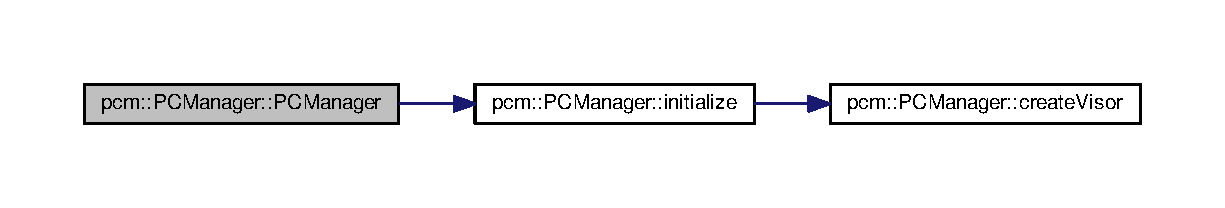
\includegraphics[width=350pt]{classpcm_1_1PCManager_ac9edd680fe7b6e9d8a2358ae8641759e_cgraph}
\end{center}
\end{figure}


\hypertarget{classpcm_1_1PCManager_af9dabc49537fa4521e7de8323a686856}{\index{pcm\-::\-P\-C\-Manager@{pcm\-::\-P\-C\-Manager}!P\-C\-Manager@{P\-C\-Manager}}
\index{P\-C\-Manager@{P\-C\-Manager}!pcm::PCManager@{pcm\-::\-P\-C\-Manager}}
\subsubsection[{P\-C\-Manager}]{\setlength{\rightskip}{0pt plus 5cm}pcm\-::\-P\-C\-Manager\-::\-P\-C\-Manager (
\begin{DoxyParamCaption}
\item[{bool}]{visualization\-Flag}
\end{DoxyParamCaption}
)}}\label{classpcm_1_1PCManager_af9dabc49537fa4521e7de8323a686856}


Definition at line 246 of file pc\-\_\-manager.\-cpp.



References initialize().



Here is the call graph for this function\-:\nopagebreak
\begin{figure}[H]
\begin{center}
\leavevmode
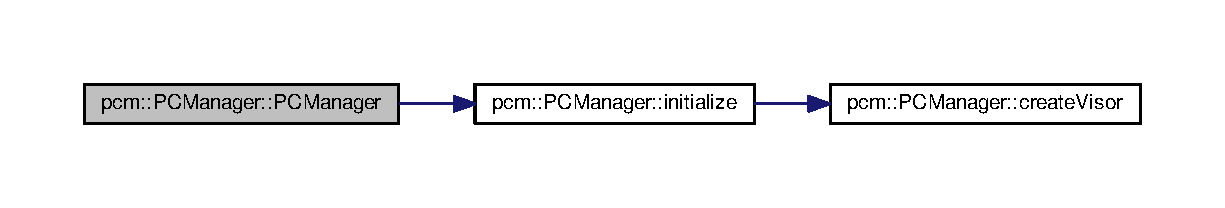
\includegraphics[width=350pt]{classpcm_1_1PCManager_af9dabc49537fa4521e7de8323a686856_cgraph}
\end{center}
\end{figure}


\hypertarget{classpcm_1_1PCManager_a488397e09fc7593a54d359ca899d6111}{\index{pcm\-::\-P\-C\-Manager@{pcm\-::\-P\-C\-Manager}!$\sim$\-P\-C\-Manager@{$\sim$\-P\-C\-Manager}}
\index{$\sim$\-P\-C\-Manager@{$\sim$\-P\-C\-Manager}!pcm::PCManager@{pcm\-::\-P\-C\-Manager}}
\subsubsection[{$\sim$\-P\-C\-Manager}]{\setlength{\rightskip}{0pt plus 5cm}pcm\-::\-P\-C\-Manager\-::$\sim$\-P\-C\-Manager (
\begin{DoxyParamCaption}
{}
\end{DoxyParamCaption}
)\hspace{0.3cm}{\ttfamily [virtual]}}}\label{classpcm_1_1PCManager_a488397e09fc7593a54d359ca899d6111}


Definition at line 251 of file pc\-\_\-manager.\-cpp.



\subsection{Member Function Documentation}
\hypertarget{classpcm_1_1PCManager_a121d34f52021c5aed1e5133688df8774}{\index{pcm\-::\-P\-C\-Manager@{pcm\-::\-P\-C\-Manager}!add\-Primitive\-Shape@{add\-Primitive\-Shape}}
\index{add\-Primitive\-Shape@{add\-Primitive\-Shape}!pcm::PCManager@{pcm\-::\-P\-C\-Manager}}
\subsubsection[{add\-Primitive\-Shape}]{\setlength{\rightskip}{0pt plus 5cm}int pcm\-::\-P\-C\-Manager\-::add\-Primitive\-Shape (
\begin{DoxyParamCaption}
\item[{string}]{shape\-Name, }
\item[{{\bf P\-C\-L\-Cloud\-Ptr}}]{cloud, }
\item[{{\bf P\-C\-L\-Normal\-Ptr}}]{norms, }
\item[{bool}]{visual\-Flag}
\end{DoxyParamCaption}
)}}\label{classpcm_1_1PCManager_a121d34f52021c5aed1e5133688df8774}
\hypertarget{classpcm_1_1PCManager_a993ec5fee41e0ce3b4f9ce403c86aaec}{\index{pcm\-::\-P\-C\-Manager@{pcm\-::\-P\-C\-Manager}!clear\-Ptimitive\-Shape@{clear\-Ptimitive\-Shape}}
\index{clear\-Ptimitive\-Shape@{clear\-Ptimitive\-Shape}!pcm::PCManager@{pcm\-::\-P\-C\-Manager}}
\subsubsection[{clear\-Ptimitive\-Shape}]{\setlength{\rightskip}{0pt plus 5cm}int pcm\-::\-P\-C\-Manager\-::clear\-Ptimitive\-Shape (
\begin{DoxyParamCaption}
{}
\end{DoxyParamCaption}
)}}\label{classpcm_1_1PCManager_a993ec5fee41e0ce3b4f9ce403c86aaec}
\hypertarget{classpcm_1_1PCManager_a91753945c3d26f6aeee6f0dc6712a7fc}{\index{pcm\-::\-P\-C\-Manager@{pcm\-::\-P\-C\-Manager}!clear\-Visor@{clear\-Visor}}
\index{clear\-Visor@{clear\-Visor}!pcm::PCManager@{pcm\-::\-P\-C\-Manager}}
\subsubsection[{clear\-Visor}]{\setlength{\rightskip}{0pt plus 5cm}void pcm\-::\-P\-C\-Manager\-::clear\-Visor (
\begin{DoxyParamCaption}
\item[{{\bf P\-C\-L\-Visualizer}}]{viewer}
\end{DoxyParamCaption}
)\hspace{0.3cm}{\ttfamily [static]}}}\label{classpcm_1_1PCManager_a91753945c3d26f6aeee6f0dc6712a7fc}


Definition at line 175 of file pc\-\_\-manager.\-cpp.

\hypertarget{classpcm_1_1PCManager_acb513ed7a3b898e398fd211bafac6f6a}{\index{pcm\-::\-P\-C\-Manager@{pcm\-::\-P\-C\-Manager}!cloud\-For\-Ros\-Msg@{cloud\-For\-Ros\-Msg}}
\index{cloud\-For\-Ros\-Msg@{cloud\-For\-Ros\-Msg}!pcm::PCManager@{pcm\-::\-P\-C\-Manager}}
\subsubsection[{cloud\-For\-Ros\-Msg}]{\setlength{\rightskip}{0pt plus 5cm}{\bf P\-C\-L\-Cloud\-Ptr} pcm\-::\-P\-C\-Manager\-::cloud\-For\-Ros\-Msg (
\begin{DoxyParamCaption}
\item[{Point\-Cloud2}]{input}
\end{DoxyParamCaption}
)\hspace{0.3cm}{\ttfamily [static]}}}\label{classpcm_1_1PCManager_acb513ed7a3b898e398fd211bafac6f6a}


Definition at line 90 of file pc\-\_\-manager.\-cpp.



Referenced by call\-Arm\-Filter(), call\-Deep\-Filter(), clusterize(), depth\-Acquisition(), ransac\-Cone\-Detaction(), ransac\-Cylinder\-Detaction(), ransac\-Plane\-Detaction(), ransac\-Sphere\-Detection(), and set\-Original\-Cloud().

\hypertarget{classpcm_1_1PCManager_aea4756e187ee152c8695dc3e7496562e}{\index{pcm\-::\-P\-C\-Manager@{pcm\-::\-P\-C\-Manager}!cloud\-For\-Ros\-Msg@{cloud\-For\-Ros\-Msg}}
\index{cloud\-For\-Ros\-Msg@{cloud\-For\-Ros\-Msg}!pcm::PCManager@{pcm\-::\-P\-C\-Manager}}
\subsubsection[{cloud\-For\-Ros\-Msg}]{\setlength{\rightskip}{0pt plus 5cm}{\bf P\-C\-L\-Cloud\-Ptr} pcm\-::\-P\-C\-Manager\-::cloud\-For\-Ros\-Msg (
\begin{DoxyParamCaption}
\item[{Point\-Cloud2\-Ptr}]{input}
\end{DoxyParamCaption}
)\hspace{0.3cm}{\ttfamily [static]}}}\label{classpcm_1_1PCManager_aea4756e187ee152c8695dc3e7496562e}


Definition at line 85 of file pc\-\_\-manager.\-cpp.

\hypertarget{classpcm_1_1PCManager_a9ec6cf99c0c34c9761fd923aace594dc}{\index{pcm\-::\-P\-C\-Manager@{pcm\-::\-P\-C\-Manager}!cloud\-To\-Ros\-Msg@{cloud\-To\-Ros\-Msg}}
\index{cloud\-To\-Ros\-Msg@{cloud\-To\-Ros\-Msg}!pcm::PCManager@{pcm\-::\-P\-C\-Manager}}
\subsubsection[{cloud\-To\-Ros\-Msg}]{\setlength{\rightskip}{0pt plus 5cm}Point\-Cloud2 pcm\-::\-P\-C\-Manager\-::cloud\-To\-Ros\-Msg (
\begin{DoxyParamCaption}
\item[{{\bf P\-C\-L\-Cloud\-Ptr}}]{input}
\end{DoxyParamCaption}
)\hspace{0.3cm}{\ttfamily [static]}}}\label{classpcm_1_1PCManager_a9ec6cf99c0c34c9761fd923aace594dc}


Definition at line 80 of file pc\-\_\-manager.\-cpp.



Referenced by call\-Arm\-Filter(), call\-Cluster\-Segmentation(), call\-Deep\-Filter(), call\-Support\-Filter(), and get\-Original\-Cloud\-Ros\-Msg().

\hypertarget{classpcm_1_1PCManager_a79353f94b8396268bea0a1358c260421}{\index{pcm\-::\-P\-C\-Manager@{pcm\-::\-P\-C\-Manager}!coefficient\-To\-Vector\-Msg@{coefficient\-To\-Vector\-Msg}}
\index{coefficient\-To\-Vector\-Msg@{coefficient\-To\-Vector\-Msg}!pcm::PCManager@{pcm\-::\-P\-C\-Manager}}
\subsubsection[{coefficient\-To\-Vector\-Msg}]{\setlength{\rightskip}{0pt plus 5cm}vector$<$ float $>$ pcm\-::\-P\-C\-Manager\-::coefficient\-To\-Vector\-Msg (
\begin{DoxyParamCaption}
\item[{Model\-Coefficients\-::\-Ptr}]{coefficients}
\end{DoxyParamCaption}
)\hspace{0.3cm}{\ttfamily [static]}}}\label{classpcm_1_1PCManager_a79353f94b8396268bea0a1358c260421}


Definition at line 112 of file pc\-\_\-manager.\-cpp.



Referenced by ransac\-Cone\-Detaction(), ransac\-Cylinder\-Detaction(), ransac\-Plane\-Detaction(), and ransac\-Sphere\-Detection().

\hypertarget{classpcm_1_1PCManager_afd0b3ae22849345d490ba27b425254a1}{\index{pcm\-::\-P\-C\-Manager@{pcm\-::\-P\-C\-Manager}!copy\-Cloud@{copy\-Cloud}}
\index{copy\-Cloud@{copy\-Cloud}!pcm::PCManager@{pcm\-::\-P\-C\-Manager}}
\subsubsection[{copy\-Cloud}]{\setlength{\rightskip}{0pt plus 5cm}{\bf P\-C\-L\-Cloud\-Ptr} pcm\-::\-P\-C\-Manager\-::copy\-Cloud (
\begin{DoxyParamCaption}
\item[{{\bf P\-C\-L\-Cloud\-Ptr}}]{input}
\end{DoxyParamCaption}
)\hspace{0.3cm}{\ttfamily [static]}}}\label{classpcm_1_1PCManager_afd0b3ae22849345d490ba27b425254a1}


Definition at line 30 of file pc\-\_\-manager.\-cpp.

\hypertarget{classpcm_1_1PCManager_aa3397d6597a17ee15d2c539631e008c2}{\index{pcm\-::\-P\-C\-Manager@{pcm\-::\-P\-C\-Manager}!copy\-Coefficients@{copy\-Coefficients}}
\index{copy\-Coefficients@{copy\-Coefficients}!pcm::PCManager@{pcm\-::\-P\-C\-Manager}}
\subsubsection[{copy\-Coefficients}]{\setlength{\rightskip}{0pt plus 5cm}Model\-Coefficients\-::\-Ptr pcm\-::\-P\-C\-Manager\-::copy\-Coefficients (
\begin{DoxyParamCaption}
\item[{Model\-Coefficients\-::\-Ptr}]{input}
\end{DoxyParamCaption}
)\hspace{0.3cm}{\ttfamily [static]}}}\label{classpcm_1_1PCManager_aa3397d6597a17ee15d2c539631e008c2}


Definition at line 49 of file pc\-\_\-manager.\-cpp.

\hypertarget{classpcm_1_1PCManager_aa580e879cf08a919167bcec0b213eb28}{\index{pcm\-::\-P\-C\-Manager@{pcm\-::\-P\-C\-Manager}!copy\-Normals@{copy\-Normals}}
\index{copy\-Normals@{copy\-Normals}!pcm::PCManager@{pcm\-::\-P\-C\-Manager}}
\subsubsection[{copy\-Normals}]{\setlength{\rightskip}{0pt plus 5cm}{\bf P\-C\-L\-Normal\-Ptr} pcm\-::\-P\-C\-Manager\-::copy\-Normals (
\begin{DoxyParamCaption}
\item[{{\bf P\-C\-L\-Normal\-Ptr}}]{input}
\end{DoxyParamCaption}
)\hspace{0.3cm}{\ttfamily [static]}}}\label{classpcm_1_1PCManager_aa580e879cf08a919167bcec0b213eb28}


Definition at line 43 of file pc\-\_\-manager.\-cpp.

\hypertarget{classpcm_1_1PCManager_a23d8e95e891a3330785375e6672ec1fe}{\index{pcm\-::\-P\-C\-Manager@{pcm\-::\-P\-C\-Manager}!create\-Visor@{create\-Visor}}
\index{create\-Visor@{create\-Visor}!pcm::PCManager@{pcm\-::\-P\-C\-Manager}}
\subsubsection[{create\-Visor}]{\setlength{\rightskip}{0pt plus 5cm}{\bf P\-C\-L\-Visualizer} pcm\-::\-P\-C\-Manager\-::create\-Visor (
\begin{DoxyParamCaption}
\item[{string}]{title}
\end{DoxyParamCaption}
)\hspace{0.3cm}{\ttfamily [static]}}}\label{classpcm_1_1PCManager_a23d8e95e891a3330785375e6672ec1fe}


Definition at line 131 of file pc\-\_\-manager.\-cpp.



Referenced by initialize(), main(), and set\-Visualization\-Flag().

\hypertarget{classpcm_1_1PCManager_ab9c66b0834ca1ef0c1c01e21400103dd}{\index{pcm\-::\-P\-C\-Manager@{pcm\-::\-P\-C\-Manager}!down\-Sampling@{down\-Sampling}}
\index{down\-Sampling@{down\-Sampling}!pcm::PCManager@{pcm\-::\-P\-C\-Manager}}
\subsubsection[{down\-Sampling}]{\setlength{\rightskip}{0pt plus 5cm}{\bf P\-C\-L\-Cloud\-Ptr} pcm\-::\-P\-C\-Manager\-::down\-Sampling (
\begin{DoxyParamCaption}
\item[{{\bf P\-C\-L\-Cloud\-Ptr}}]{input}
\end{DoxyParamCaption}
)\hspace{0.3cm}{\ttfamily [static]}}}\label{classpcm_1_1PCManager_ab9c66b0834ca1ef0c1c01e21400103dd}


Definition at line 55 of file pc\-\_\-manager.\-cpp.



References D\-E\-F\-A\-U\-L\-T\-\_\-\-D\-O\-W\-S\-E\-A\-M\-P\-L\-I\-G\-\_\-\-R\-A\-T\-E.



Referenced by depth\-Acquisition(), down\-Sampling(), and set\-Original\-Cloud().

\hypertarget{classpcm_1_1PCManager_a32a6c0ad1f2d23e48ddb4302be7d14c5}{\index{pcm\-::\-P\-C\-Manager@{pcm\-::\-P\-C\-Manager}!down\-Sampling@{down\-Sampling}}
\index{down\-Sampling@{down\-Sampling}!pcm::PCManager@{pcm\-::\-P\-C\-Manager}}
\subsubsection[{down\-Sampling}]{\setlength{\rightskip}{0pt plus 5cm}{\bf P\-C\-L\-Cloud\-Ptr} pcm\-::\-P\-C\-Manager\-::down\-Sampling (
\begin{DoxyParamCaption}
\item[{{\bf P\-C\-L\-Cloud\-Ptr}}]{input, }
\item[{float}]{span}
\end{DoxyParamCaption}
)\hspace{0.3cm}{\ttfamily [static]}}}\label{classpcm_1_1PCManager_a32a6c0ad1f2d23e48ddb4302be7d14c5}


Definition at line 58 of file pc\-\_\-manager.\-cpp.



References down\-Sampling().



Here is the call graph for this function\-:\nopagebreak
\begin{figure}[H]
\begin{center}
\leavevmode
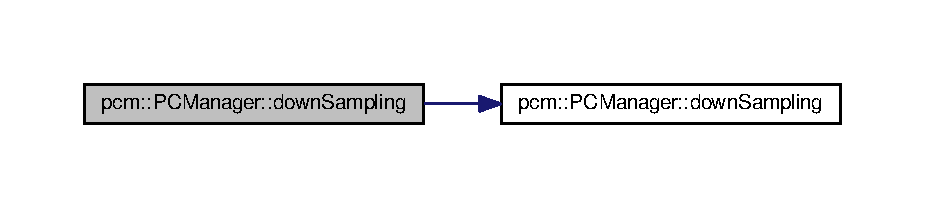
\includegraphics[width=350pt]{classpcm_1_1PCManager_a32a6c0ad1f2d23e48ddb4302be7d14c5_cgraph}
\end{center}
\end{figure}


\hypertarget{classpcm_1_1PCManager_a30723a3f4808cd2a161b58c0888d5dfa}{\index{pcm\-::\-P\-C\-Manager@{pcm\-::\-P\-C\-Manager}!down\-Sampling@{down\-Sampling}}
\index{down\-Sampling@{down\-Sampling}!pcm::PCManager@{pcm\-::\-P\-C\-Manager}}
\subsubsection[{down\-Sampling}]{\setlength{\rightskip}{0pt plus 5cm}{\bf P\-C\-L\-Cloud\-Ptr} pcm\-::\-P\-C\-Manager\-::down\-Sampling (
\begin{DoxyParamCaption}
\item[{{\bf P\-C\-L\-Cloud\-Ptr}}]{input, }
\item[{float}]{span\-X, }
\item[{float}]{span\-Y, }
\item[{float}]{span\-Z}
\end{DoxyParamCaption}
)\hspace{0.3cm}{\ttfamily [static]}}}\label{classpcm_1_1PCManager_a30723a3f4808cd2a161b58c0888d5dfa}


Definition at line 61 of file pc\-\_\-manager.\-cpp.



References pcm\-::sor.

\hypertarget{classpcm_1_1PCManager_ab2cdef39cbe4f3d6c3660d873bd9a38e}{\index{pcm\-::\-P\-C\-Manager@{pcm\-::\-P\-C\-Manager}!estimate\-Normal@{estimate\-Normal}}
\index{estimate\-Normal@{estimate\-Normal}!pcm::PCManager@{pcm\-::\-P\-C\-Manager}}
\subsubsection[{estimate\-Normal}]{\setlength{\rightskip}{0pt plus 5cm}{\bf P\-C\-L\-Normal\-Ptr} pcm\-::\-P\-C\-Manager\-::estimate\-Normal (
\begin{DoxyParamCaption}
\item[{{\bf P\-C\-L\-Cloud\-Ptr}}]{input}
\end{DoxyParamCaption}
)\hspace{0.3cm}{\ttfamily [static]}}}\label{classpcm_1_1PCManager_ab2cdef39cbe4f3d6c3660d873bd9a38e}


Definition at line 68 of file pc\-\_\-manager.\-cpp.



References D\-E\-F\-A\-U\-L\-T\-\_\-\-N\-O\-R\-M\-\_\-\-S\-E\-A\-R\-C\-H.



Referenced by depth\-Acquisition(), and set\-Original\-Cloud().

\hypertarget{classpcm_1_1PCManager_a7cad87bdc0a16f5b4b6108259ace90d3}{\index{pcm\-::\-P\-C\-Manager@{pcm\-::\-P\-C\-Manager}!estimate\-Normal@{estimate\-Normal}}
\index{estimate\-Normal@{estimate\-Normal}!pcm::PCManager@{pcm\-::\-P\-C\-Manager}}
\subsubsection[{estimate\-Normal}]{\setlength{\rightskip}{0pt plus 5cm}{\bf P\-C\-L\-Normal\-Ptr} pcm\-::\-P\-C\-Manager\-::estimate\-Normal (
\begin{DoxyParamCaption}
\item[{{\bf P\-C\-L\-Cloud\-Ptr}}]{input, }
\item[{int}]{search}
\end{DoxyParamCaption}
)\hspace{0.3cm}{\ttfamily [static]}}}\label{classpcm_1_1PCManager_a7cad87bdc0a16f5b4b6108259ace90d3}


Definition at line 71 of file pc\-\_\-manager.\-cpp.



References pcm\-::ne, and pcm\-::tree().



Here is the call graph for this function\-:\nopagebreak
\begin{figure}[H]
\begin{center}
\leavevmode
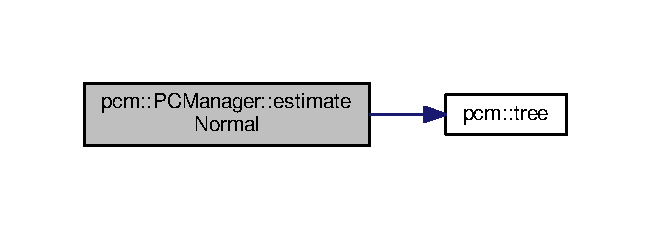
\includegraphics[width=312pt]{classpcm_1_1PCManager_a7cad87bdc0a16f5b4b6108259ace90d3_cgraph}
\end{center}
\end{figure}


\hypertarget{classpcm_1_1PCManager_a881ed083a239069699906a669492fc1d}{\index{pcm\-::\-P\-C\-Manager@{pcm\-::\-P\-C\-Manager}!get\-Cloud\-From\-Idx@{get\-Cloud\-From\-Idx}}
\index{get\-Cloud\-From\-Idx@{get\-Cloud\-From\-Idx}!pcm::PCManager@{pcm\-::\-P\-C\-Manager}}
\subsubsection[{get\-Cloud\-From\-Idx}]{\setlength{\rightskip}{0pt plus 5cm}vector$<$ {\bf P\-C\-L\-Cloud\-Ptr} $>$ pcm\-::\-P\-C\-Manager\-::get\-Cloud\-From\-Idx (
\begin{DoxyParamCaption}
\item[{{\bf P\-C\-L\-Cloud\-Ptr}}]{original\-Cloud, }
\item[{{\bf Primitive\-Idx\-Ptr}}]{indices}
\end{DoxyParamCaption}
)\hspace{0.3cm}{\ttfamily [static]}}}\label{classpcm_1_1PCManager_a881ed083a239069699906a669492fc1d}


Definition at line 181 of file pc\-\_\-manager.\-cpp.



Referenced by get\-Cloud\-From\-Idx().

\hypertarget{classpcm_1_1PCManager_a73da6d454214f5ba90d978b50ff4438f}{\index{pcm\-::\-P\-C\-Manager@{pcm\-::\-P\-C\-Manager}!get\-Cloud\-From\-Idx@{get\-Cloud\-From\-Idx}}
\index{get\-Cloud\-From\-Idx@{get\-Cloud\-From\-Idx}!pcm::PCManager@{pcm\-::\-P\-C\-Manager}}
\subsubsection[{get\-Cloud\-From\-Idx}]{\setlength{\rightskip}{0pt plus 5cm}vector$<$ {\bf P\-C\-L\-Cloud\-Ptr} $>$ pcm\-::\-P\-C\-Manager\-::get\-Cloud\-From\-Idx (
\begin{DoxyParamCaption}
\item[{{\bf Primitive\-Idx\-Ptr}}]{indices}
\end{DoxyParamCaption}
)}}\label{classpcm_1_1PCManager_a73da6d454214f5ba90d978b50ff4438f}


Definition at line 235 of file pc\-\_\-manager.\-cpp.



References get\-Cloud\-From\-Idx(), and original\-Cloud.



Here is the call graph for this function\-:\nopagebreak
\begin{figure}[H]
\begin{center}
\leavevmode
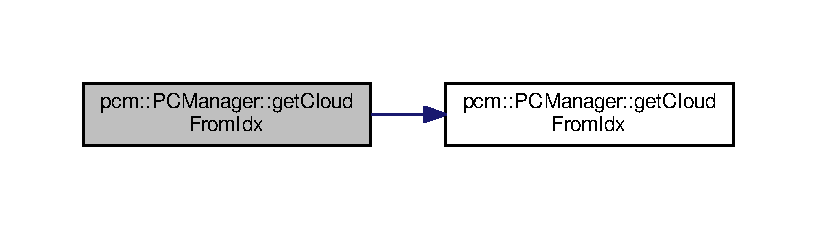
\includegraphics[width=350pt]{classpcm_1_1PCManager_a73da6d454214f5ba90d978b50ff4438f_cgraph}
\end{center}
\end{figure}


\hypertarget{classpcm_1_1PCManager_ac1a98146a63dfd36626a16ed1a50098a}{\index{pcm\-::\-P\-C\-Manager@{pcm\-::\-P\-C\-Manager}!get\-Fomratted\-Data@{get\-Fomratted\-Data}}
\index{get\-Fomratted\-Data@{get\-Fomratted\-Data}!pcm::PCManager@{pcm\-::\-P\-C\-Manager}}
\subsubsection[{get\-Fomratted\-Data}]{\setlength{\rightskip}{0pt plus 5cm}string pcm\-::\-P\-C\-Manager\-::get\-Fomratted\-Data (
\begin{DoxyParamCaption}
{}
\end{DoxyParamCaption}
)\hspace{0.3cm}{\ttfamily [static]}}}\label{classpcm_1_1PCManager_ac1a98146a63dfd36626a16ed1a50098a}


Definition at line 121 of file pc\-\_\-manager.\-cpp.



Referenced by srvm\-::get\-Path\-Parameter().

\hypertarget{classpcm_1_1PCManager_a3f26dafa3a2808b3ee927d9724f9c9a6}{\index{pcm\-::\-P\-C\-Manager@{pcm\-::\-P\-C\-Manager}!get\-Original\-Cloud@{get\-Original\-Cloud}}
\index{get\-Original\-Cloud@{get\-Original\-Cloud}!pcm::PCManager@{pcm\-::\-P\-C\-Manager}}
\subsubsection[{get\-Original\-Cloud}]{\setlength{\rightskip}{0pt plus 5cm}{\bf P\-C\-L\-Cloud\-Ptr} pcm\-::\-P\-C\-Manager\-::get\-Original\-Cloud (
\begin{DoxyParamCaption}
{}
\end{DoxyParamCaption}
)}}\label{classpcm_1_1PCManager_a3f26dafa3a2808b3ee927d9724f9c9a6}


Definition at line 289 of file pc\-\_\-manager.\-cpp.



References original\-Cloud.

\hypertarget{classpcm_1_1PCManager_a1a11270e78e96c38f9c40985529fc5b6}{\index{pcm\-::\-P\-C\-Manager@{pcm\-::\-P\-C\-Manager}!get\-Original\-Cloud\-Ros\-Msg@{get\-Original\-Cloud\-Ros\-Msg}}
\index{get\-Original\-Cloud\-Ros\-Msg@{get\-Original\-Cloud\-Ros\-Msg}!pcm::PCManager@{pcm\-::\-P\-C\-Manager}}
\subsubsection[{get\-Original\-Cloud\-Ros\-Msg}]{\setlength{\rightskip}{0pt plus 5cm}Point\-Cloud2 pcm\-::\-P\-C\-Manager\-::get\-Original\-Cloud\-Ros\-Msg (
\begin{DoxyParamCaption}
{}
\end{DoxyParamCaption}
)}}\label{classpcm_1_1PCManager_a1a11270e78e96c38f9c40985529fc5b6}


Definition at line 292 of file pc\-\_\-manager.\-cpp.



References cloud\-To\-Ros\-Msg(), and original\-Cloud.



Here is the call graph for this function\-:\nopagebreak
\begin{figure}[H]
\begin{center}
\leavevmode
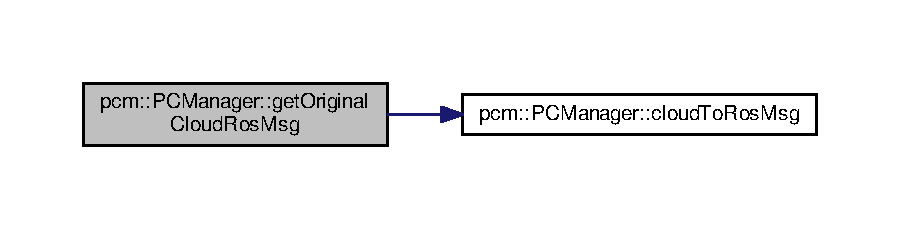
\includegraphics[width=350pt]{classpcm_1_1PCManager_a1a11270e78e96c38f9c40985529fc5b6_cgraph}
\end{center}
\end{figure}


\hypertarget{classpcm_1_1PCManager_a471d768a4a32a8d8992c688fc6fc2f58}{\index{pcm\-::\-P\-C\-Manager@{pcm\-::\-P\-C\-Manager}!get\-Original\-Normal@{get\-Original\-Normal}}
\index{get\-Original\-Normal@{get\-Original\-Normal}!pcm::PCManager@{pcm\-::\-P\-C\-Manager}}
\subsubsection[{get\-Original\-Normal}]{\setlength{\rightskip}{0pt plus 5cm}{\bf P\-C\-L\-Normal\-Ptr} pcm\-::\-P\-C\-Manager\-::get\-Original\-Normal (
\begin{DoxyParamCaption}
{}
\end{DoxyParamCaption}
)}}\label{classpcm_1_1PCManager_a471d768a4a32a8d8992c688fc6fc2f58}


Definition at line 296 of file pc\-\_\-manager.\-cpp.



References original\-Norms.

\hypertarget{classpcm_1_1PCManager_a01a64a81b18e5bc984c46910d2a881be}{\index{pcm\-::\-P\-C\-Manager@{pcm\-::\-P\-C\-Manager}!get\-Original\-Normal\-Ros\-Msg@{get\-Original\-Normal\-Ros\-Msg}}
\index{get\-Original\-Normal\-Ros\-Msg@{get\-Original\-Normal\-Ros\-Msg}!pcm::PCManager@{pcm\-::\-P\-C\-Manager}}
\subsubsection[{get\-Original\-Normal\-Ros\-Msg}]{\setlength{\rightskip}{0pt plus 5cm}Point\-Cloud2 pcm\-::\-P\-C\-Manager\-::get\-Original\-Normal\-Ros\-Msg (
\begin{DoxyParamCaption}
{}
\end{DoxyParamCaption}
)}}\label{classpcm_1_1PCManager_a01a64a81b18e5bc984c46910d2a881be}


Definition at line 299 of file pc\-\_\-manager.\-cpp.



References norm\-To\-Ros\-Msg(), and original\-Norms.



Here is the call graph for this function\-:\nopagebreak
\begin{figure}[H]
\begin{center}
\leavevmode
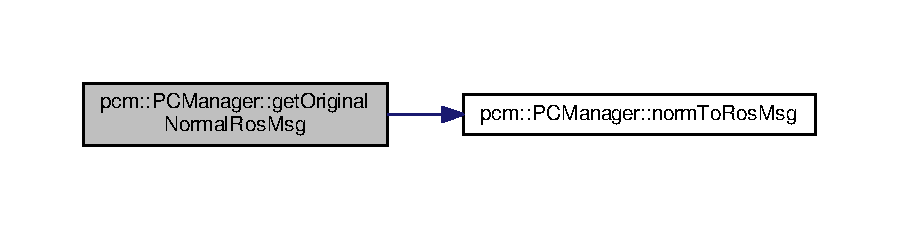
\includegraphics[width=350pt]{classpcm_1_1PCManager_a01a64a81b18e5bc984c46910d2a881be_cgraph}
\end{center}
\end{figure}


\hypertarget{classpcm_1_1PCManager_a3575801a21b3fd9613dd57cb97ffaa47}{\index{pcm\-::\-P\-C\-Manager@{pcm\-::\-P\-C\-Manager}!get\-Primitive\-Shape@{get\-Primitive\-Shape}}
\index{get\-Primitive\-Shape@{get\-Primitive\-Shape}!pcm::PCManager@{pcm\-::\-P\-C\-Manager}}
\subsubsection[{get\-Primitive\-Shape}]{\setlength{\rightskip}{0pt plus 5cm}{\bf P\-C\-Primitive\-Ptr} pcm\-::\-P\-C\-Manager\-::get\-Primitive\-Shape (
\begin{DoxyParamCaption}
\item[{int}]{idx}
\end{DoxyParamCaption}
)}}\label{classpcm_1_1PCManager_a3575801a21b3fd9613dd57cb97ffaa47}
\hypertarget{classpcm_1_1PCManager_ac1cfd8753c305e761a3c5914f74cca7b}{\index{pcm\-::\-P\-C\-Manager@{pcm\-::\-P\-C\-Manager}!get\-Visor@{get\-Visor}}
\index{get\-Visor@{get\-Visor}!pcm::PCManager@{pcm\-::\-P\-C\-Manager}}
\subsubsection[{get\-Visor}]{\setlength{\rightskip}{0pt plus 5cm}{\bf P\-C\-L\-Visualizer} pcm\-::\-P\-C\-Manager\-::get\-Visor (
\begin{DoxyParamCaption}
{}
\end{DoxyParamCaption}
)}}\label{classpcm_1_1PCManager_ac1cfd8753c305e761a3c5914f74cca7b}


Definition at line 306 of file pc\-\_\-manager.\-cpp.



References visor.

\hypertarget{classpcm_1_1PCManager_a4d419e1bf7e35f8f3ddbb7f640c50a72}{\index{pcm\-::\-P\-C\-Manager@{pcm\-::\-P\-C\-Manager}!get\-Visualization\-Flag@{get\-Visualization\-Flag}}
\index{get\-Visualization\-Flag@{get\-Visualization\-Flag}!pcm::PCManager@{pcm\-::\-P\-C\-Manager}}
\subsubsection[{get\-Visualization\-Flag}]{\setlength{\rightskip}{0pt plus 5cm}bool pcm\-::\-P\-C\-Manager\-::get\-Visualization\-Flag (
\begin{DoxyParamCaption}
{}
\end{DoxyParamCaption}
)}}\label{classpcm_1_1PCManager_a4d419e1bf7e35f8f3ddbb7f640c50a72}


Definition at line 303 of file pc\-\_\-manager.\-cpp.



References visualization\-Flag.

\hypertarget{classpcm_1_1PCManager_ad79130d97fa80234552372c3e7e81ee3}{\index{pcm\-::\-P\-C\-Manager@{pcm\-::\-P\-C\-Manager}!initialize@{initialize}}
\index{initialize@{initialize}!pcm::PCManager@{pcm\-::\-P\-C\-Manager}}
\subsubsection[{initialize}]{\setlength{\rightskip}{0pt plus 5cm}void pcm\-::\-P\-C\-Manager\-::initialize (
\begin{DoxyParamCaption}
\item[{bool}]{visualization\-Flag}
\end{DoxyParamCaption}
)\hspace{0.3cm}{\ttfamily [private]}}}\label{classpcm_1_1PCManager_ad79130d97fa80234552372c3e7e81ee3}


Definition at line 347 of file pc\-\_\-manager.\-cpp.



References create\-Visor(), D\-E\-F\-A\-U\-L\-T\-\_\-\-V\-I\-S\-U\-A\-L\-I\-Z\-E\-R\-\_\-\-T\-I\-T\-L\-E, visor, and visualization\-Flag.



Referenced by P\-C\-Manager().



Here is the call graph for this function\-:\nopagebreak
\begin{figure}[H]
\begin{center}
\leavevmode
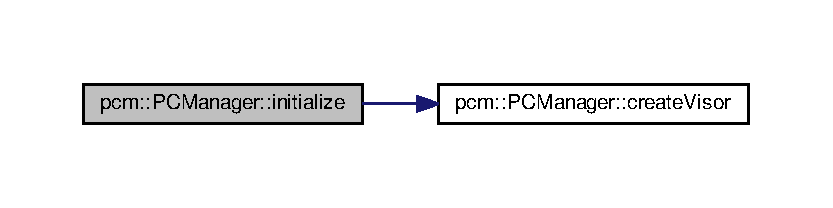
\includegraphics[width=350pt]{classpcm_1_1PCManager_ad79130d97fa80234552372c3e7e81ee3_cgraph}
\end{center}
\end{figure}


\hypertarget{classpcm_1_1PCManager_ab473f60dc622465a1c3ff77000f0803f}{\index{pcm\-::\-P\-C\-Manager@{pcm\-::\-P\-C\-Manager}!inlier\-To\-Vector\-Msg@{inlier\-To\-Vector\-Msg}}
\index{inlier\-To\-Vector\-Msg@{inlier\-To\-Vector\-Msg}!pcm::PCManager@{pcm\-::\-P\-C\-Manager}}
\subsubsection[{inlier\-To\-Vector\-Msg}]{\setlength{\rightskip}{0pt plus 5cm}vector$<$ int $>$ pcm\-::\-P\-C\-Manager\-::inlier\-To\-Vector\-Msg (
\begin{DoxyParamCaption}
\item[{Point\-Indices\-::\-Ptr}]{inliers}
\end{DoxyParamCaption}
)\hspace{0.3cm}{\ttfamily [static]}}}\label{classpcm_1_1PCManager_ab473f60dc622465a1c3ff77000f0803f}


Definition at line 105 of file pc\-\_\-manager.\-cpp.



Referenced by ransac\-Cone\-Detaction(), ransac\-Cylinder\-Detaction(), ransac\-Plane\-Detaction(), and ransac\-Sphere\-Detection().

\hypertarget{classpcm_1_1PCManager_a75f790855ce87d24293bb3a8e4a453c9}{\index{pcm\-::\-P\-C\-Manager@{pcm\-::\-P\-C\-Manager}!norm\-For\-Ros\-Msg@{norm\-For\-Ros\-Msg}}
\index{norm\-For\-Ros\-Msg@{norm\-For\-Ros\-Msg}!pcm::PCManager@{pcm\-::\-P\-C\-Manager}}
\subsubsection[{norm\-For\-Ros\-Msg}]{\setlength{\rightskip}{0pt plus 5cm}{\bf P\-C\-L\-Normal\-Ptr} pcm\-::\-P\-C\-Manager\-::norm\-For\-Ros\-Msg (
\begin{DoxyParamCaption}
\item[{Point\-Cloud2}]{input}
\end{DoxyParamCaption}
)\hspace{0.3cm}{\ttfamily [static]}}}\label{classpcm_1_1PCManager_a75f790855ce87d24293bb3a8e4a453c9}


Definition at line 100 of file pc\-\_\-manager.\-cpp.



Referenced by ransac\-Cone\-Detaction(), ransac\-Cylinder\-Detaction(), ransac\-Plane\-Detaction(), and ransac\-Sphere\-Detection().

\hypertarget{classpcm_1_1PCManager_aad8d4dd6c1bb761213134760be5673c3}{\index{pcm\-::\-P\-C\-Manager@{pcm\-::\-P\-C\-Manager}!norm\-To\-Ros\-Msg@{norm\-To\-Ros\-Msg}}
\index{norm\-To\-Ros\-Msg@{norm\-To\-Ros\-Msg}!pcm::PCManager@{pcm\-::\-P\-C\-Manager}}
\subsubsection[{norm\-To\-Ros\-Msg}]{\setlength{\rightskip}{0pt plus 5cm}Point\-Cloud2 pcm\-::\-P\-C\-Manager\-::norm\-To\-Ros\-Msg (
\begin{DoxyParamCaption}
\item[{{\bf P\-C\-L\-Normal\-Ptr}}]{input}
\end{DoxyParamCaption}
)\hspace{0.3cm}{\ttfamily [static]}}}\label{classpcm_1_1PCManager_aad8d4dd6c1bb761213134760be5673c3}


Definition at line 95 of file pc\-\_\-manager.\-cpp.



Referenced by call\-Support\-Filter(), and get\-Original\-Normal\-Ros\-Msg().

\hypertarget{classpcm_1_1PCManager_a2144cf37b92d58e902f7e6b1dcb6984d}{\index{pcm\-::\-P\-C\-Manager@{pcm\-::\-P\-C\-Manager}!set\-Original\-Cloud@{set\-Original\-Cloud}}
\index{set\-Original\-Cloud@{set\-Original\-Cloud}!pcm::PCManager@{pcm\-::\-P\-C\-Manager}}
\subsubsection[{set\-Original\-Cloud}]{\setlength{\rightskip}{0pt plus 5cm}void pcm\-::\-P\-C\-Manager\-::set\-Original\-Cloud (
\begin{DoxyParamCaption}
\item[{{\bf P\-C\-L\-Cloud\-Ptr}}]{cloud}
\end{DoxyParamCaption}
)}}\label{classpcm_1_1PCManager_a2144cf37b92d58e902f7e6b1dcb6984d}


Definition at line 312 of file pc\-\_\-manager.\-cpp.



References D\-E\-F\-A\-U\-L\-T\-\_\-\-D\-O\-W\-S\-E\-A\-M\-P\-L\-I\-G\-\_\-\-R\-A\-T\-E, and D\-E\-F\-A\-U\-L\-T\-\_\-\-N\-O\-R\-M\-\_\-\-S\-E\-A\-R\-C\-H.



Referenced by set\-Original\-Cloud().

\hypertarget{classpcm_1_1PCManager_ac277411304ee22415cdeaad26cd4721c}{\index{pcm\-::\-P\-C\-Manager@{pcm\-::\-P\-C\-Manager}!set\-Original\-Cloud@{set\-Original\-Cloud}}
\index{set\-Original\-Cloud@{set\-Original\-Cloud}!pcm::PCManager@{pcm\-::\-P\-C\-Manager}}
\subsubsection[{set\-Original\-Cloud}]{\setlength{\rightskip}{0pt plus 5cm}void pcm\-::\-P\-C\-Manager\-::set\-Original\-Cloud (
\begin{DoxyParamCaption}
\item[{{\bf P\-C\-L\-Cloud\-Ptr}}]{cloud, }
\item[{int}]{norm\-Search, }
\item[{float}]{down\-Span\-X, }
\item[{float}]{down\-Span\-Y, }
\item[{float}]{down\-Span\-Z}
\end{DoxyParamCaption}
)}}\label{classpcm_1_1PCManager_ac277411304ee22415cdeaad26cd4721c}


Definition at line 315 of file pc\-\_\-manager.\-cpp.



References down\-Sampling(), estimate\-Normal(), original\-Cloud, and original\-Norms.



Here is the call graph for this function\-:\nopagebreak
\begin{figure}[H]
\begin{center}
\leavevmode
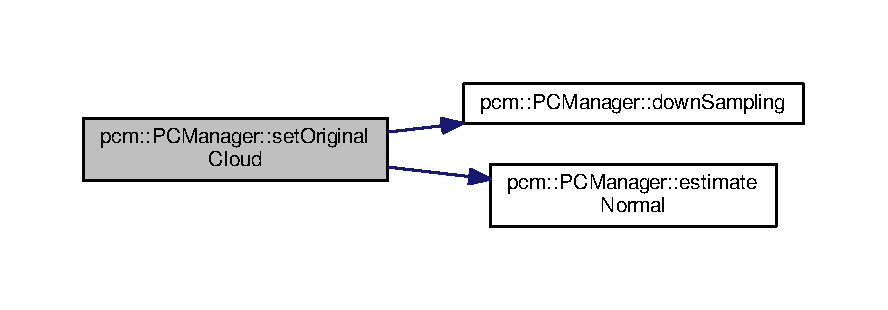
\includegraphics[width=350pt]{classpcm_1_1PCManager_ac277411304ee22415cdeaad26cd4721c_cgraph}
\end{center}
\end{figure}


\hypertarget{classpcm_1_1PCManager_a8eafedbcc9cb93380e826bc45bff1410}{\index{pcm\-::\-P\-C\-Manager@{pcm\-::\-P\-C\-Manager}!set\-Original\-Cloud@{set\-Original\-Cloud}}
\index{set\-Original\-Cloud@{set\-Original\-Cloud}!pcm::PCManager@{pcm\-::\-P\-C\-Manager}}
\subsubsection[{set\-Original\-Cloud}]{\setlength{\rightskip}{0pt plus 5cm}void pcm\-::\-P\-C\-Manager\-::set\-Original\-Cloud (
\begin{DoxyParamCaption}
\item[{Point\-Cloud2\-Ptr}]{cloud}
\end{DoxyParamCaption}
)}}\label{classpcm_1_1PCManager_a8eafedbcc9cb93380e826bc45bff1410}


Definition at line 323 of file pc\-\_\-manager.\-cpp.



References D\-E\-F\-A\-U\-L\-T\-\_\-\-D\-O\-W\-S\-E\-A\-M\-P\-L\-I\-G\-\_\-\-R\-A\-T\-E, D\-E\-F\-A\-U\-L\-T\-\_\-\-N\-O\-R\-M\-\_\-\-S\-E\-A\-R\-C\-H, and set\-Original\-Cloud().



Here is the call graph for this function\-:\nopagebreak
\begin{figure}[H]
\begin{center}
\leavevmode
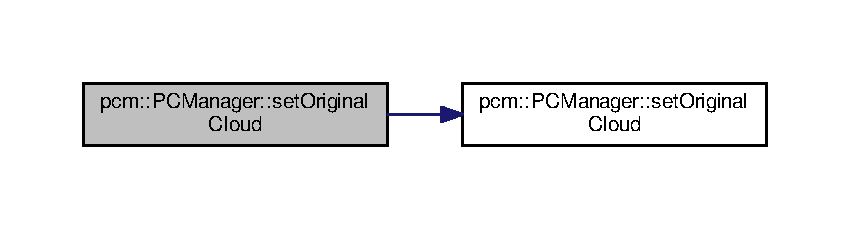
\includegraphics[width=350pt]{classpcm_1_1PCManager_a8eafedbcc9cb93380e826bc45bff1410_cgraph}
\end{center}
\end{figure}


\hypertarget{classpcm_1_1PCManager_aa5bd3ef55ff3ef39cded25351c7b4d9e}{\index{pcm\-::\-P\-C\-Manager@{pcm\-::\-P\-C\-Manager}!set\-Original\-Cloud@{set\-Original\-Cloud}}
\index{set\-Original\-Cloud@{set\-Original\-Cloud}!pcm::PCManager@{pcm\-::\-P\-C\-Manager}}
\subsubsection[{set\-Original\-Cloud}]{\setlength{\rightskip}{0pt plus 5cm}void pcm\-::\-P\-C\-Manager\-::set\-Original\-Cloud (
\begin{DoxyParamCaption}
\item[{Point\-Cloud2\-Ptr}]{cloud, }
\item[{int}]{norm\-Search, }
\item[{float}]{down\-Span\-X, }
\item[{float}]{down\-Span\-Y, }
\item[{float}]{down\-Span\-Z}
\end{DoxyParamCaption}
)}}\label{classpcm_1_1PCManager_aa5bd3ef55ff3ef39cded25351c7b4d9e}


Definition at line 326 of file pc\-\_\-manager.\-cpp.



References cloud\-For\-Ros\-Msg(), and set\-Original\-Cloud().



Here is the call graph for this function\-:\nopagebreak
\begin{figure}[H]
\begin{center}
\leavevmode
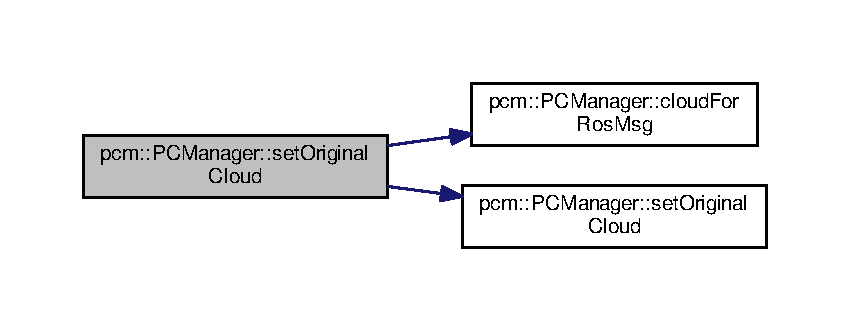
\includegraphics[width=350pt]{classpcm_1_1PCManager_aa5bd3ef55ff3ef39cded25351c7b4d9e_cgraph}
\end{center}
\end{figure}


\hypertarget{classpcm_1_1PCManager_a40c79e3197147779d263b95fd3617974}{\index{pcm\-::\-P\-C\-Manager@{pcm\-::\-P\-C\-Manager}!set\-Visualization\-Flag@{set\-Visualization\-Flag}}
\index{set\-Visualization\-Flag@{set\-Visualization\-Flag}!pcm::PCManager@{pcm\-::\-P\-C\-Manager}}
\subsubsection[{set\-Visualization\-Flag}]{\setlength{\rightskip}{0pt plus 5cm}void pcm\-::\-P\-C\-Manager\-::set\-Visualization\-Flag (
\begin{DoxyParamCaption}
\item[{bool}]{flag}
\end{DoxyParamCaption}
)}}\label{classpcm_1_1PCManager_a40c79e3197147779d263b95fd3617974}


Definition at line 330 of file pc\-\_\-manager.\-cpp.



References create\-Visor(), D\-E\-F\-A\-U\-L\-T\-\_\-\-V\-I\-S\-U\-A\-L\-I\-Z\-E\-R\-\_\-\-T\-I\-T\-L\-E, visor, and visualization\-Flag.



Here is the call graph for this function\-:\nopagebreak
\begin{figure}[H]
\begin{center}
\leavevmode
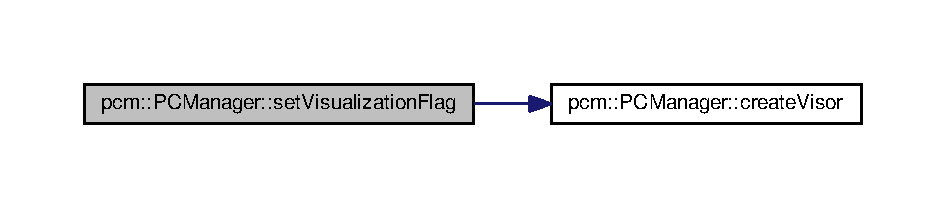
\includegraphics[width=350pt]{classpcm_1_1PCManager_a40c79e3197147779d263b95fd3617974_cgraph}
\end{center}
\end{figure}


\hypertarget{classpcm_1_1PCManager_a8b6dfcce0709c29f63a82c4dfa6ef6e6}{\index{pcm\-::\-P\-C\-Manager@{pcm\-::\-P\-C\-Manager}!update\-Visor@{update\-Visor}}
\index{update\-Visor@{update\-Visor}!pcm::PCManager@{pcm\-::\-P\-C\-Manager}}
\subsubsection[{update\-Visor}]{\setlength{\rightskip}{0pt plus 5cm}void pcm\-::\-P\-C\-Manager\-::update\-Visor (
\begin{DoxyParamCaption}
\item[{{\bf P\-C\-L\-Visualizer}}]{viewer, }
\item[{{\bf P\-C\-L\-Cloud\-Ptr}}]{cloud, }
\item[{int}]{R, }
\item[{int}]{G, }
\item[{int}]{B, }
\item[{string}]{name}
\end{DoxyParamCaption}
)\hspace{0.3cm}{\ttfamily [static]}}}\label{classpcm_1_1PCManager_a8b6dfcce0709c29f63a82c4dfa6ef6e6}


Definition at line 152 of file pc\-\_\-manager.\-cpp.



References V\-I\-S\-U\-A\-L\-I\-Z\-E\-R\-\_\-\-P\-O\-I\-N\-T\-\_\-\-S\-I\-Z\-E.



Referenced by depth\-Acquisition(), ransac\-Cone\-Detaction(), ransac\-Cylinder\-Detaction(), and update\-Visor().

\hypertarget{classpcm_1_1PCManager_af6498d518bd4eb1ad5f724849a851e90}{\index{pcm\-::\-P\-C\-Manager@{pcm\-::\-P\-C\-Manager}!update\-Visor@{update\-Visor}}
\index{update\-Visor@{update\-Visor}!pcm::PCManager@{pcm\-::\-P\-C\-Manager}}
\subsubsection[{update\-Visor}]{\setlength{\rightskip}{0pt plus 5cm}void pcm\-::\-P\-C\-Manager\-::update\-Visor (
\begin{DoxyParamCaption}
\item[{{\bf P\-C\-L\-Visualizer}}]{viewer, }
\item[{{\bf P\-C\-L\-Cloud\-Ptr}}]{cloud, }
\item[{string}]{name}
\end{DoxyParamCaption}
)\hspace{0.3cm}{\ttfamily [static]}}}\label{classpcm_1_1PCManager_af6498d518bd4eb1ad5f724849a851e90}


Definition at line 159 of file pc\-\_\-manager.\-cpp.



References update\-Visor().



Here is the call graph for this function\-:\nopagebreak
\begin{figure}[H]
\begin{center}
\leavevmode
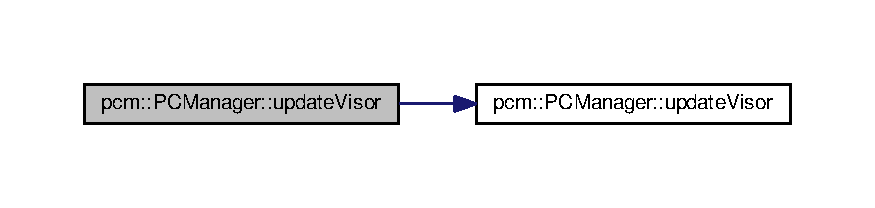
\includegraphics[width=350pt]{classpcm_1_1PCManager_af6498d518bd4eb1ad5f724849a851e90_cgraph}
\end{center}
\end{figure}


\hypertarget{classpcm_1_1PCManager_ae65d976eaaf49a2db303e91d30279cb0}{\index{pcm\-::\-P\-C\-Manager@{pcm\-::\-P\-C\-Manager}!update\-Visor@{update\-Visor}}
\index{update\-Visor@{update\-Visor}!pcm::PCManager@{pcm\-::\-P\-C\-Manager}}
\subsubsection[{update\-Visor}]{\setlength{\rightskip}{0pt plus 5cm}void pcm\-::\-P\-C\-Manager\-::update\-Visor (
\begin{DoxyParamCaption}
\item[{{\bf P\-C\-L\-Visualizer}}]{viewer, }
\item[{{\bf P\-C\-L\-Cloud\-Ptr}}]{cloud, }
\item[{{\bf P\-C\-L\-Normal\-Ptr}}]{normals, }
\item[{int}]{R, }
\item[{int}]{G, }
\item[{int}]{B, }
\item[{string}]{name}
\end{DoxyParamCaption}
)\hspace{0.3cm}{\ttfamily [static]}}}\label{classpcm_1_1PCManager_ae65d976eaaf49a2db303e91d30279cb0}


Definition at line 163 of file pc\-\_\-manager.\-cpp.



References D\-E\-F\-A\-U\-L\-T\-\_\-\-N\-O\-R\-M\-\_\-\-L\-E\-V\-E\-L, D\-E\-F\-A\-U\-L\-T\-\_\-\-N\-O\-R\-M\-\_\-\-N\-A\-M\-E\-\_\-\-S\-U\-F\-F\-I\-X, D\-E\-F\-A\-U\-L\-T\-\_\-\-N\-O\-R\-M\-\_\-\-S\-C\-A\-L\-E, and V\-I\-S\-U\-A\-L\-I\-Z\-E\-R\-\_\-\-P\-O\-I\-N\-T\-\_\-\-S\-I\-Z\-E.

\hypertarget{classpcm_1_1PCManager_a183ac77330de59a04c4de18e3270fbb8}{\index{pcm\-::\-P\-C\-Manager@{pcm\-::\-P\-C\-Manager}!update\-Visor@{update\-Visor}}
\index{update\-Visor@{update\-Visor}!pcm::PCManager@{pcm\-::\-P\-C\-Manager}}
\subsubsection[{update\-Visor}]{\setlength{\rightskip}{0pt plus 5cm}void pcm\-::\-P\-C\-Manager\-::update\-Visor (
\begin{DoxyParamCaption}
\item[{{\bf P\-C\-L\-Visualizer}}]{viewer, }
\item[{{\bf P\-C\-L\-Cloud\-Ptr}}]{cloud, }
\item[{{\bf P\-C\-L\-Normal\-Ptr}}]{normals, }
\item[{string}]{name}
\end{DoxyParamCaption}
)\hspace{0.3cm}{\ttfamily [static]}}}\label{classpcm_1_1PCManager_a183ac77330de59a04c4de18e3270fbb8}


Definition at line 172 of file pc\-\_\-manager.\-cpp.



References update\-Visor().



Here is the call graph for this function\-:\nopagebreak
\begin{figure}[H]
\begin{center}
\leavevmode
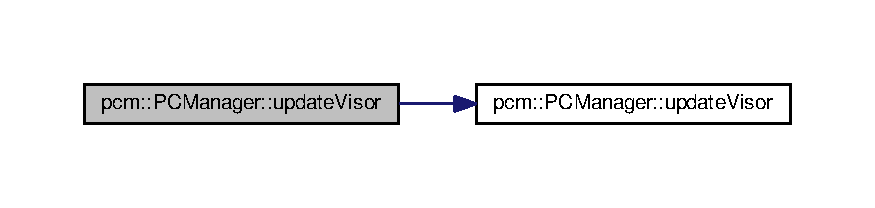
\includegraphics[width=350pt]{classpcm_1_1PCManager_a183ac77330de59a04c4de18e3270fbb8_cgraph}
\end{center}
\end{figure}


\hypertarget{classpcm_1_1PCManager_a4e249a3ef952e13bf941ccb90ff6c1f9}{\index{pcm\-::\-P\-C\-Manager@{pcm\-::\-P\-C\-Manager}!update\-Visor@{update\-Visor}}
\index{update\-Visor@{update\-Visor}!pcm::PCManager@{pcm\-::\-P\-C\-Manager}}
\subsubsection[{update\-Visor}]{\setlength{\rightskip}{0pt plus 5cm}void pcm\-::\-P\-C\-Manager\-::update\-Visor (
\begin{DoxyParamCaption}
\item[{{\bf P\-C\-L\-Visualizer}}]{viewer, }
\item[{Point\-X\-Y\-Z}]{point, }
\item[{int}]{R, }
\item[{int}]{G, }
\item[{int}]{B, }
\item[{string}]{name}
\end{DoxyParamCaption}
)\hspace{0.3cm}{\ttfamily [static]}}}\label{classpcm_1_1PCManager_a4e249a3ef952e13bf941ccb90ff6c1f9}


Definition at line 139 of file pc\-\_\-manager.\-cpp.



References V\-I\-S\-U\-A\-L\-I\-Z\-E\-R\-\_\-\-P\-O\-I\-N\-T\-\_\-\-S\-I\-Z\-E\-\_\-\-B\-I\-G.

\hypertarget{classpcm_1_1PCManager_a684c37d6b0637aa3bb08fe47d67b9fb6}{\index{pcm\-::\-P\-C\-Manager@{pcm\-::\-P\-C\-Manager}!update\-Visor@{update\-Visor}}
\index{update\-Visor@{update\-Visor}!pcm::PCManager@{pcm\-::\-P\-C\-Manager}}
\subsubsection[{update\-Visor}]{\setlength{\rightskip}{0pt plus 5cm}void pcm\-::\-P\-C\-Manager\-::update\-Visor (
\begin{DoxyParamCaption}
\item[{{\bf P\-C\-L\-Visualizer}}]{viewer, }
\item[{Point\-X\-Y\-Z}]{point, }
\item[{string}]{name}
\end{DoxyParamCaption}
)\hspace{0.3cm}{\ttfamily [static]}}}\label{classpcm_1_1PCManager_a684c37d6b0637aa3bb08fe47d67b9fb6}


Definition at line 148 of file pc\-\_\-manager.\-cpp.



References update\-Visor().



Here is the call graph for this function\-:\nopagebreak
\begin{figure}[H]
\begin{center}
\leavevmode
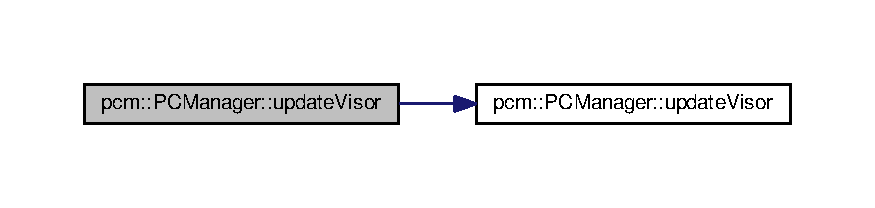
\includegraphics[width=350pt]{classpcm_1_1PCManager_a684c37d6b0637aa3bb08fe47d67b9fb6_cgraph}
\end{center}
\end{figure}


\hypertarget{classpcm_1_1PCManager_ad73afae724cbba84e40ed94ac4123864}{\index{pcm\-::\-P\-C\-Manager@{pcm\-::\-P\-C\-Manager}!visualize@{visualize}}
\index{visualize@{visualize}!pcm::PCManager@{pcm\-::\-P\-C\-Manager}}
\subsubsection[{visualize}]{\setlength{\rightskip}{0pt plus 5cm}void pcm\-::\-P\-C\-Manager\-::visualize (
\begin{DoxyParamCaption}
{}
\end{DoxyParamCaption}
)}}\label{classpcm_1_1PCManager_ad73afae724cbba84e40ed94ac4123864}
\hypertarget{classpcm_1_1PCManager_a43f25363aa71aafc754a2ae42c832797}{\index{pcm\-::\-P\-C\-Manager@{pcm\-::\-P\-C\-Manager}!write\-To\-File@{write\-To\-File}}
\index{write\-To\-File@{write\-To\-File}!pcm::PCManager@{pcm\-::\-P\-C\-Manager}}
\subsubsection[{write\-To\-File}]{\setlength{\rightskip}{0pt plus 5cm}bool pcm\-::\-P\-C\-Manager\-::write\-To\-File (
\begin{DoxyParamCaption}
\item[{string}]{txt, }
\item[{string}]{file\-Path, }
\item[{bool}]{append}
\end{DoxyParamCaption}
)\hspace{0.3cm}{\ttfamily [static]}}}\label{classpcm_1_1PCManager_a43f25363aa71aafc754a2ae42c832797}


Definition at line 215 of file pc\-\_\-manager.\-cpp.



Referenced by depth\-Acquisition(), and main().



\subsection{Member Data Documentation}
\hypertarget{classpcm_1_1PCManager_aceb117314161d997ffcd102c4a2e3668}{\index{pcm\-::\-P\-C\-Manager@{pcm\-::\-P\-C\-Manager}!D\-E\-F\-A\-U\-L\-T\-\_\-\-C\-L\-O\-U\-D\-\_\-\-N\-A\-M\-E\-\_\-\-S\-U\-F\-F\-I\-X@{D\-E\-F\-A\-U\-L\-T\-\_\-\-C\-L\-O\-U\-D\-\_\-\-N\-A\-M\-E\-\_\-\-S\-U\-F\-F\-I\-X}}
\index{D\-E\-F\-A\-U\-L\-T\-\_\-\-C\-L\-O\-U\-D\-\_\-\-N\-A\-M\-E\-\_\-\-S\-U\-F\-F\-I\-X@{D\-E\-F\-A\-U\-L\-T\-\_\-\-C\-L\-O\-U\-D\-\_\-\-N\-A\-M\-E\-\_\-\-S\-U\-F\-F\-I\-X}!pcm::PCManager@{pcm\-::\-P\-C\-Manager}}
\subsubsection[{D\-E\-F\-A\-U\-L\-T\-\_\-\-C\-L\-O\-U\-D\-\_\-\-N\-A\-M\-E\-\_\-\-S\-U\-F\-F\-I\-X}]{\setlength{\rightskip}{0pt plus 5cm}const string pcm\-::\-P\-C\-Manager\-::\-D\-E\-F\-A\-U\-L\-T\-\_\-\-C\-L\-O\-U\-D\-\_\-\-N\-A\-M\-E\-\_\-\-S\-U\-F\-F\-I\-X = \char`\"{}\-\_\-cloud\char`\"{}\hspace{0.3cm}{\ttfamily [static]}}}\label{classpcm_1_1PCManager_aceb117314161d997ffcd102c4a2e3668}


Definition at line 112 of file pc\-\_\-manager.\-h.

\hypertarget{classpcm_1_1PCManager_a21a35f215779915eda52dbf8d77f1e9f}{\index{pcm\-::\-P\-C\-Manager@{pcm\-::\-P\-C\-Manager}!D\-E\-F\-A\-U\-L\-T\-\_\-\-D\-O\-W\-S\-E\-A\-M\-P\-L\-I\-G\-\_\-\-R\-A\-T\-E@{D\-E\-F\-A\-U\-L\-T\-\_\-\-D\-O\-W\-S\-E\-A\-M\-P\-L\-I\-G\-\_\-\-R\-A\-T\-E}}
\index{D\-E\-F\-A\-U\-L\-T\-\_\-\-D\-O\-W\-S\-E\-A\-M\-P\-L\-I\-G\-\_\-\-R\-A\-T\-E@{D\-E\-F\-A\-U\-L\-T\-\_\-\-D\-O\-W\-S\-E\-A\-M\-P\-L\-I\-G\-\_\-\-R\-A\-T\-E}!pcm::PCManager@{pcm\-::\-P\-C\-Manager}}
\subsubsection[{D\-E\-F\-A\-U\-L\-T\-\_\-\-D\-O\-W\-S\-E\-A\-M\-P\-L\-I\-G\-\_\-\-R\-A\-T\-E}]{\setlength{\rightskip}{0pt plus 5cm}const float pcm\-::\-P\-C\-Manager\-::\-D\-E\-F\-A\-U\-L\-T\-\_\-\-D\-O\-W\-S\-E\-A\-M\-P\-L\-I\-G\-\_\-\-R\-A\-T\-E = 0.\-01f\hspace{0.3cm}{\ttfamily [static]}}}\label{classpcm_1_1PCManager_a21a35f215779915eda52dbf8d77f1e9f}


Definition at line 120 of file pc\-\_\-manager.\-h.



Referenced by down\-Sampling(), and set\-Original\-Cloud().

\hypertarget{classpcm_1_1PCManager_af4959e1ce5dc2650aab2754472a18ac8}{\index{pcm\-::\-P\-C\-Manager@{pcm\-::\-P\-C\-Manager}!D\-E\-F\-A\-U\-L\-T\-\_\-\-N\-O\-R\-M\-\_\-\-L\-E\-V\-E\-L@{D\-E\-F\-A\-U\-L\-T\-\_\-\-N\-O\-R\-M\-\_\-\-L\-E\-V\-E\-L}}
\index{D\-E\-F\-A\-U\-L\-T\-\_\-\-N\-O\-R\-M\-\_\-\-L\-E\-V\-E\-L@{D\-E\-F\-A\-U\-L\-T\-\_\-\-N\-O\-R\-M\-\_\-\-L\-E\-V\-E\-L}!pcm::PCManager@{pcm\-::\-P\-C\-Manager}}
\subsubsection[{D\-E\-F\-A\-U\-L\-T\-\_\-\-N\-O\-R\-M\-\_\-\-L\-E\-V\-E\-L}]{\setlength{\rightskip}{0pt plus 5cm}const int pcm\-::\-P\-C\-Manager\-::\-D\-E\-F\-A\-U\-L\-T\-\_\-\-N\-O\-R\-M\-\_\-\-L\-E\-V\-E\-L = 5\hspace{0.3cm}{\ttfamily [static]}}}\label{classpcm_1_1PCManager_af4959e1ce5dc2650aab2754472a18ac8}


Definition at line 115 of file pc\-\_\-manager.\-h.



Referenced by update\-Visor().

\hypertarget{classpcm_1_1PCManager_a7cacb2df053d19d4d6d346a0b45082d9}{\index{pcm\-::\-P\-C\-Manager@{pcm\-::\-P\-C\-Manager}!D\-E\-F\-A\-U\-L\-T\-\_\-\-N\-O\-R\-M\-\_\-\-N\-A\-M\-E\-\_\-\-S\-U\-F\-F\-I\-X@{D\-E\-F\-A\-U\-L\-T\-\_\-\-N\-O\-R\-M\-\_\-\-N\-A\-M\-E\-\_\-\-S\-U\-F\-F\-I\-X}}
\index{D\-E\-F\-A\-U\-L\-T\-\_\-\-N\-O\-R\-M\-\_\-\-N\-A\-M\-E\-\_\-\-S\-U\-F\-F\-I\-X@{D\-E\-F\-A\-U\-L\-T\-\_\-\-N\-O\-R\-M\-\_\-\-N\-A\-M\-E\-\_\-\-S\-U\-F\-F\-I\-X}!pcm::PCManager@{pcm\-::\-P\-C\-Manager}}
\subsubsection[{D\-E\-F\-A\-U\-L\-T\-\_\-\-N\-O\-R\-M\-\_\-\-N\-A\-M\-E\-\_\-\-S\-U\-F\-F\-I\-X}]{\setlength{\rightskip}{0pt plus 5cm}const string pcm\-::\-P\-C\-Manager\-::\-D\-E\-F\-A\-U\-L\-T\-\_\-\-N\-O\-R\-M\-\_\-\-N\-A\-M\-E\-\_\-\-S\-U\-F\-F\-I\-X = \char`\"{}\-\_\-normal\char`\"{}\hspace{0.3cm}{\ttfamily [static]}}}\label{classpcm_1_1PCManager_a7cacb2df053d19d4d6d346a0b45082d9}


Definition at line 113 of file pc\-\_\-manager.\-h.



Referenced by update\-Visor().

\hypertarget{classpcm_1_1PCManager_a95ec8d073d4a573b550a44031f986608}{\index{pcm\-::\-P\-C\-Manager@{pcm\-::\-P\-C\-Manager}!D\-E\-F\-A\-U\-L\-T\-\_\-\-N\-O\-R\-M\-\_\-\-S\-C\-A\-L\-E@{D\-E\-F\-A\-U\-L\-T\-\_\-\-N\-O\-R\-M\-\_\-\-S\-C\-A\-L\-E}}
\index{D\-E\-F\-A\-U\-L\-T\-\_\-\-N\-O\-R\-M\-\_\-\-S\-C\-A\-L\-E@{D\-E\-F\-A\-U\-L\-T\-\_\-\-N\-O\-R\-M\-\_\-\-S\-C\-A\-L\-E}!pcm::PCManager@{pcm\-::\-P\-C\-Manager}}
\subsubsection[{D\-E\-F\-A\-U\-L\-T\-\_\-\-N\-O\-R\-M\-\_\-\-S\-C\-A\-L\-E}]{\setlength{\rightskip}{0pt plus 5cm}const float pcm\-::\-P\-C\-Manager\-::\-D\-E\-F\-A\-U\-L\-T\-\_\-\-N\-O\-R\-M\-\_\-\-S\-C\-A\-L\-E = 0.\-02f\hspace{0.3cm}{\ttfamily [static]}}}\label{classpcm_1_1PCManager_a95ec8d073d4a573b550a44031f986608}


Definition at line 116 of file pc\-\_\-manager.\-h.



Referenced by update\-Visor().

\hypertarget{classpcm_1_1PCManager_a507973d100aef370fd7a2feeda4fb273}{\index{pcm\-::\-P\-C\-Manager@{pcm\-::\-P\-C\-Manager}!D\-E\-F\-A\-U\-L\-T\-\_\-\-N\-O\-R\-M\-\_\-\-S\-E\-A\-R\-C\-H@{D\-E\-F\-A\-U\-L\-T\-\_\-\-N\-O\-R\-M\-\_\-\-S\-E\-A\-R\-C\-H}}
\index{D\-E\-F\-A\-U\-L\-T\-\_\-\-N\-O\-R\-M\-\_\-\-S\-E\-A\-R\-C\-H@{D\-E\-F\-A\-U\-L\-T\-\_\-\-N\-O\-R\-M\-\_\-\-S\-E\-A\-R\-C\-H}!pcm::PCManager@{pcm\-::\-P\-C\-Manager}}
\subsubsection[{D\-E\-F\-A\-U\-L\-T\-\_\-\-N\-O\-R\-M\-\_\-\-S\-E\-A\-R\-C\-H}]{\setlength{\rightskip}{0pt plus 5cm}const int pcm\-::\-P\-C\-Manager\-::\-D\-E\-F\-A\-U\-L\-T\-\_\-\-N\-O\-R\-M\-\_\-\-S\-E\-A\-R\-C\-H = 50\hspace{0.3cm}{\ttfamily [static]}}}\label{classpcm_1_1PCManager_a507973d100aef370fd7a2feeda4fb273}


Definition at line 119 of file pc\-\_\-manager.\-h.



Referenced by estimate\-Normal(), and set\-Original\-Cloud().

\hypertarget{classpcm_1_1PCManager_adec1cf4832f6f63548aa3a4001077ec5}{\index{pcm\-::\-P\-C\-Manager@{pcm\-::\-P\-C\-Manager}!D\-E\-F\-A\-U\-L\-T\-\_\-\-O\-R\-I\-G\-I\-N\-A\-L\-\_\-\-C\-L\-O\-U\-D\-\_\-\-V\-I\-E\-W\-E\-R\-\_\-\-N\-A\-M\-E@{D\-E\-F\-A\-U\-L\-T\-\_\-\-O\-R\-I\-G\-I\-N\-A\-L\-\_\-\-C\-L\-O\-U\-D\-\_\-\-V\-I\-E\-W\-E\-R\-\_\-\-N\-A\-M\-E}}
\index{D\-E\-F\-A\-U\-L\-T\-\_\-\-O\-R\-I\-G\-I\-N\-A\-L\-\_\-\-C\-L\-O\-U\-D\-\_\-\-V\-I\-E\-W\-E\-R\-\_\-\-N\-A\-M\-E@{D\-E\-F\-A\-U\-L\-T\-\_\-\-O\-R\-I\-G\-I\-N\-A\-L\-\_\-\-C\-L\-O\-U\-D\-\_\-\-V\-I\-E\-W\-E\-R\-\_\-\-N\-A\-M\-E}!pcm::PCManager@{pcm\-::\-P\-C\-Manager}}
\subsubsection[{D\-E\-F\-A\-U\-L\-T\-\_\-\-O\-R\-I\-G\-I\-N\-A\-L\-\_\-\-C\-L\-O\-U\-D\-\_\-\-V\-I\-E\-W\-E\-R\-\_\-\-N\-A\-M\-E}]{\setlength{\rightskip}{0pt plus 5cm}const string pcm\-::\-P\-C\-Manager\-::\-D\-E\-F\-A\-U\-L\-T\-\_\-\-O\-R\-I\-G\-I\-N\-A\-L\-\_\-\-C\-L\-O\-U\-D\-\_\-\-V\-I\-E\-W\-E\-R\-\_\-\-N\-A\-M\-E = \char`\"{}original\char`\"{}\hspace{0.3cm}{\ttfamily [static]}}}\label{classpcm_1_1PCManager_adec1cf4832f6f63548aa3a4001077ec5}


Definition at line 114 of file pc\-\_\-manager.\-h.

\hypertarget{classpcm_1_1PCManager_aaddf643dfa30897c1851d97cc6732e73}{\index{pcm\-::\-P\-C\-Manager@{pcm\-::\-P\-C\-Manager}!D\-E\-F\-A\-U\-L\-T\-\_\-\-V\-I\-S\-U\-A\-L\-I\-Z\-A\-T\-I\-O\-N\-\_\-\-F\-L\-A\-G@{D\-E\-F\-A\-U\-L\-T\-\_\-\-V\-I\-S\-U\-A\-L\-I\-Z\-A\-T\-I\-O\-N\-\_\-\-F\-L\-A\-G}}
\index{D\-E\-F\-A\-U\-L\-T\-\_\-\-V\-I\-S\-U\-A\-L\-I\-Z\-A\-T\-I\-O\-N\-\_\-\-F\-L\-A\-G@{D\-E\-F\-A\-U\-L\-T\-\_\-\-V\-I\-S\-U\-A\-L\-I\-Z\-A\-T\-I\-O\-N\-\_\-\-F\-L\-A\-G}!pcm::PCManager@{pcm\-::\-P\-C\-Manager}}
\subsubsection[{D\-E\-F\-A\-U\-L\-T\-\_\-\-V\-I\-S\-U\-A\-L\-I\-Z\-A\-T\-I\-O\-N\-\_\-\-F\-L\-A\-G}]{\setlength{\rightskip}{0pt plus 5cm}const bool pcm\-::\-P\-C\-Manager\-::\-D\-E\-F\-A\-U\-L\-T\-\_\-\-V\-I\-S\-U\-A\-L\-I\-Z\-A\-T\-I\-O\-N\-\_\-\-F\-L\-A\-G = false\hspace{0.3cm}{\ttfamily [static]}}}\label{classpcm_1_1PCManager_aaddf643dfa30897c1851d97cc6732e73}


Definition at line 109 of file pc\-\_\-manager.\-h.



Referenced by P\-C\-Manager().

\hypertarget{classpcm_1_1PCManager_a87b7714f198b56306c4fc8f10b71ba27}{\index{pcm\-::\-P\-C\-Manager@{pcm\-::\-P\-C\-Manager}!D\-E\-F\-A\-U\-L\-T\-\_\-\-V\-I\-S\-U\-A\-L\-I\-Z\-E\-R\-\_\-\-T\-I\-T\-L\-E@{D\-E\-F\-A\-U\-L\-T\-\_\-\-V\-I\-S\-U\-A\-L\-I\-Z\-E\-R\-\_\-\-T\-I\-T\-L\-E}}
\index{D\-E\-F\-A\-U\-L\-T\-\_\-\-V\-I\-S\-U\-A\-L\-I\-Z\-E\-R\-\_\-\-T\-I\-T\-L\-E@{D\-E\-F\-A\-U\-L\-T\-\_\-\-V\-I\-S\-U\-A\-L\-I\-Z\-E\-R\-\_\-\-T\-I\-T\-L\-E}!pcm::PCManager@{pcm\-::\-P\-C\-Manager}}
\subsubsection[{D\-E\-F\-A\-U\-L\-T\-\_\-\-V\-I\-S\-U\-A\-L\-I\-Z\-E\-R\-\_\-\-T\-I\-T\-L\-E}]{\setlength{\rightskip}{0pt plus 5cm}const string pcm\-::\-P\-C\-Manager\-::\-D\-E\-F\-A\-U\-L\-T\-\_\-\-V\-I\-S\-U\-A\-L\-I\-Z\-E\-R\-\_\-\-T\-I\-T\-L\-E = \char`\"{}Point\-Cloud {\bf manager}\char`\"{}\hspace{0.3cm}{\ttfamily [static]}}}\label{classpcm_1_1PCManager_a87b7714f198b56306c4fc8f10b71ba27}


Definition at line 117 of file pc\-\_\-manager.\-h.



Referenced by initialize(), and set\-Visualization\-Flag().

\hypertarget{classpcm_1_1PCManager_a2f7fc5bdae476711dbd0b79fccca14f3}{\index{pcm\-::\-P\-C\-Manager@{pcm\-::\-P\-C\-Manager}!original\-Cloud@{original\-Cloud}}
\index{original\-Cloud@{original\-Cloud}!pcm::PCManager@{pcm\-::\-P\-C\-Manager}}
\subsubsection[{original\-Cloud}]{\setlength{\rightskip}{0pt plus 5cm}{\bf P\-C\-L\-Cloud\-Ptr} pcm\-::\-P\-C\-Manager\-::original\-Cloud\hspace{0.3cm}{\ttfamily [private]}}}\label{classpcm_1_1PCManager_a2f7fc5bdae476711dbd0b79fccca14f3}


Definition at line 29 of file pc\-\_\-manager.\-h.



Referenced by get\-Cloud\-From\-Idx(), get\-Original\-Cloud(), get\-Original\-Cloud\-Ros\-Msg(), and set\-Original\-Cloud().

\hypertarget{classpcm_1_1PCManager_a87eb9af97f2704d0bae90e27ef483462}{\index{pcm\-::\-P\-C\-Manager@{pcm\-::\-P\-C\-Manager}!original\-Norms@{original\-Norms}}
\index{original\-Norms@{original\-Norms}!pcm::PCManager@{pcm\-::\-P\-C\-Manager}}
\subsubsection[{original\-Norms}]{\setlength{\rightskip}{0pt plus 5cm}{\bf P\-C\-L\-Normal\-Ptr} pcm\-::\-P\-C\-Manager\-::original\-Norms\hspace{0.3cm}{\ttfamily [private]}}}\label{classpcm_1_1PCManager_a87eb9af97f2704d0bae90e27ef483462}


Definition at line 30 of file pc\-\_\-manager.\-h.



Referenced by get\-Original\-Normal(), get\-Original\-Normal\-Ros\-Msg(), and set\-Original\-Cloud().

\hypertarget{classpcm_1_1PCManager_a0306662716691bbf53aaa55c768d582d}{\index{pcm\-::\-P\-C\-Manager@{pcm\-::\-P\-C\-Manager}!primitive\-List@{primitive\-List}}
\index{primitive\-List@{primitive\-List}!pcm::PCManager@{pcm\-::\-P\-C\-Manager}}
\subsubsection[{primitive\-List}]{\setlength{\rightskip}{0pt plus 5cm}vector$<$ {\bf P\-C\-Primitive\-Ptr}$>$ pcm\-::\-P\-C\-Manager\-::primitive\-List\hspace{0.3cm}{\ttfamily [private]}}}\label{classpcm_1_1PCManager_a0306662716691bbf53aaa55c768d582d}


Definition at line 35 of file pc\-\_\-manager.\-h.

\hypertarget{classpcm_1_1PCManager_a114916eb53bacdd547331d0de53d6ced}{\index{pcm\-::\-P\-C\-Manager@{pcm\-::\-P\-C\-Manager}!visor@{visor}}
\index{visor@{visor}!pcm::PCManager@{pcm\-::\-P\-C\-Manager}}
\subsubsection[{visor}]{\setlength{\rightskip}{0pt plus 5cm}{\bf P\-C\-L\-Visualizer} pcm\-::\-P\-C\-Manager\-::visor\hspace{0.3cm}{\ttfamily [private]}}}\label{classpcm_1_1PCManager_a114916eb53bacdd547331d0de53d6ced}


Definition at line 32 of file pc\-\_\-manager.\-h.



Referenced by get\-Visor(), initialize(), and set\-Visualization\-Flag().

\hypertarget{classpcm_1_1PCManager_af2215813be83c41ca788a40614c9fadb}{\index{pcm\-::\-P\-C\-Manager@{pcm\-::\-P\-C\-Manager}!visualization\-Flag@{visualization\-Flag}}
\index{visualization\-Flag@{visualization\-Flag}!pcm::PCManager@{pcm\-::\-P\-C\-Manager}}
\subsubsection[{visualization\-Flag}]{\setlength{\rightskip}{0pt plus 5cm}bool pcm\-::\-P\-C\-Manager\-::visualization\-Flag\hspace{0.3cm}{\ttfamily [private]}}}\label{classpcm_1_1PCManager_af2215813be83c41ca788a40614c9fadb}


Definition at line 33 of file pc\-\_\-manager.\-h.



Referenced by get\-Visualization\-Flag(), initialize(), and set\-Visualization\-Flag().

\hypertarget{classpcm_1_1PCManager_abb62ef760d6d8436c18cac80bb111898}{\index{pcm\-::\-P\-C\-Manager@{pcm\-::\-P\-C\-Manager}!V\-I\-S\-U\-A\-L\-I\-Z\-E\-R\-\_\-\-P\-O\-I\-N\-T\-\_\-\-S\-I\-Z\-E@{V\-I\-S\-U\-A\-L\-I\-Z\-E\-R\-\_\-\-P\-O\-I\-N\-T\-\_\-\-S\-I\-Z\-E}}
\index{V\-I\-S\-U\-A\-L\-I\-Z\-E\-R\-\_\-\-P\-O\-I\-N\-T\-\_\-\-S\-I\-Z\-E@{V\-I\-S\-U\-A\-L\-I\-Z\-E\-R\-\_\-\-P\-O\-I\-N\-T\-\_\-\-S\-I\-Z\-E}!pcm::PCManager@{pcm\-::\-P\-C\-Manager}}
\subsubsection[{V\-I\-S\-U\-A\-L\-I\-Z\-E\-R\-\_\-\-P\-O\-I\-N\-T\-\_\-\-S\-I\-Z\-E}]{\setlength{\rightskip}{0pt plus 5cm}const int pcm\-::\-P\-C\-Manager\-::\-V\-I\-S\-U\-A\-L\-I\-Z\-E\-R\-\_\-\-P\-O\-I\-N\-T\-\_\-\-S\-I\-Z\-E = 3\hspace{0.3cm}{\ttfamily [static]}}}\label{classpcm_1_1PCManager_abb62ef760d6d8436c18cac80bb111898}


Definition at line 110 of file pc\-\_\-manager.\-h.



Referenced by update\-Visor().

\hypertarget{classpcm_1_1PCManager_a53820f1bdb5fc94830c0a04334916d12}{\index{pcm\-::\-P\-C\-Manager@{pcm\-::\-P\-C\-Manager}!V\-I\-S\-U\-A\-L\-I\-Z\-E\-R\-\_\-\-P\-O\-I\-N\-T\-\_\-\-S\-I\-Z\-E\-\_\-\-B\-I\-G@{V\-I\-S\-U\-A\-L\-I\-Z\-E\-R\-\_\-\-P\-O\-I\-N\-T\-\_\-\-S\-I\-Z\-E\-\_\-\-B\-I\-G}}
\index{V\-I\-S\-U\-A\-L\-I\-Z\-E\-R\-\_\-\-P\-O\-I\-N\-T\-\_\-\-S\-I\-Z\-E\-\_\-\-B\-I\-G@{V\-I\-S\-U\-A\-L\-I\-Z\-E\-R\-\_\-\-P\-O\-I\-N\-T\-\_\-\-S\-I\-Z\-E\-\_\-\-B\-I\-G}!pcm::PCManager@{pcm\-::\-P\-C\-Manager}}
\subsubsection[{V\-I\-S\-U\-A\-L\-I\-Z\-E\-R\-\_\-\-P\-O\-I\-N\-T\-\_\-\-S\-I\-Z\-E\-\_\-\-B\-I\-G}]{\setlength{\rightskip}{0pt plus 5cm}const int pcm\-::\-P\-C\-Manager\-::\-V\-I\-S\-U\-A\-L\-I\-Z\-E\-R\-\_\-\-P\-O\-I\-N\-T\-\_\-\-S\-I\-Z\-E\-\_\-\-B\-I\-G = 10\hspace{0.3cm}{\ttfamily [static]}}}\label{classpcm_1_1PCManager_a53820f1bdb5fc94830c0a04334916d12}


Definition at line 111 of file pc\-\_\-manager.\-h.



Referenced by update\-Visor().



The documentation for this class was generated from the following files\-:\begin{DoxyCompactItemize}
\item 
src/point\-\_\-cloud\-\_\-library/\hyperlink{pc__manager_8h}{pc\-\_\-manager.\-h}\item 
src/point\-\_\-cloud\-\_\-library/\hyperlink{pc__manager_8cpp}{pc\-\_\-manager.\-cpp}\end{DoxyCompactItemize}

\hypertarget{classpcp_1_1PCPrimitive}{\section{pcp\-:\-:P\-C\-Primitive Class Reference}
\label{classpcp_1_1PCPrimitive}\index{pcp\-::\-P\-C\-Primitive@{pcp\-::\-P\-C\-Primitive}}
}


{\ttfamily \#include $<$pc\-\_\-primitive.\-h$>$}

\subsection*{Public Member Functions}
\begin{DoxyCompactItemize}
\item 
\hyperlink{classpcp_1_1PCPrimitive_a00c270f938ac1f76c1252422e1f1424f}{P\-C\-Primitive} (string shapename, int shape\-Mapidx, bool visual\-Flag, \hyperlink{pc__primitive_8h_aa14a240c8d999c4f56133c0f70e88783}{P\-C\-L\-Cloud\-Ptr} cloud, \hyperlink{pc__primitive_8h_a1bc38ce8b0c26e5f2d28fae9f3e3ea97}{P\-C\-L\-Normal\-Ptr} norms)
\item 
virtual \hyperlink{classpcp_1_1PCPrimitive_a3a4da7e50a67144bc1b5b4dfd376b72e}{$\sim$\-P\-C\-Primitive} ()
\item 
string \hyperlink{classpcp_1_1PCPrimitive_a9f507218fd4c442d0daa4938e2e71c10}{get\-Shape\-Name} ()
\item 
string \hyperlink{classpcp_1_1PCPrimitive_ae6a97bc88b8cc7e83476413c73e01aeb}{get\-Visualization\-Name} ()
\item 
bool \hyperlink{classpcp_1_1PCPrimitive_ad92a83f976c6aac8125c7c8997633f21}{get\-Visualization\-Flag} ()
\item 
int \hyperlink{classpcp_1_1PCPrimitive_a1251deb8c39370d0ed5e7d2c7290063f}{get\-Shape\-Mapidx} ()
\item 
\hyperlink{pc__primitive_8h_a02a7c0cdfcd324f1b5b87ce549fdbe10}{P\-C\-L\-Cloud} \hyperlink{classpcp_1_1PCPrimitive_ac774df2f9bb393e9a1491da1b0131d4f}{get\-Primitive\-Cloud} ()
\item 
\hyperlink{pc__primitive_8h_abe81b5e6ffcc0ceb1b95b0489419027d}{P\-C\-L\-Normal} \hyperlink{classpcp_1_1PCPrimitive_aafdd30869b5e09e394d70efebe5eac2a}{get\-Primitive\-Normal} ()
\end{DoxyCompactItemize}
\subsection*{Static Public Attributes}
\begin{DoxyCompactItemize}
\item 
static const string \hyperlink{classpcp_1_1PCPrimitive_a640bb9e84b55d900e6edbaef8b938d6e}{D\-E\-F\-A\-U\-L\-T\-\_\-\-S\-H\-A\-P\-E\-\_\-\-N\-A\-M\-E\-\_\-\-P\-L\-A\-N\-E} = \char`\"{}plane\char`\"{}
\item 
static const string \hyperlink{classpcp_1_1PCPrimitive_ab54a8fb25b750b3808d652f25161ba02}{D\-E\-F\-A\-U\-L\-T\-\_\-\-S\-H\-A\-P\-E\-\_\-\-N\-A\-M\-E\-\_\-\-C\-L\-U\-S\-T\-E\-R} = \char`\"{}cluster\char`\"{}
\item 
static const string \hyperlink{classpcp_1_1PCPrimitive_a9dc28983a955e1f9b1813a15e4260386}{D\-E\-F\-A\-U\-L\-T\-\_\-\-V\-I\-S\-U\-A\-L\-I\-Z\-A\-T\-I\-O\-N\-\_\-\-N\-A\-M\-E\-\_\-\-S\-E\-P\-A\-R\-A\-T\-O\-R} = \char`\"{}-\/\char`\"{}
\end{DoxyCompactItemize}
\subsection*{Private Member Functions}
\begin{DoxyCompactItemize}
\item 
string \hyperlink{classpcp_1_1PCPrimitive_a0764e20850fd7392f657d1cc43e8ec77}{get\-Visualization\-Name\-From\-Tag} (int idx)
\item 
Model\-Coefficients \hyperlink{classpcp_1_1PCPrimitive_a2d8fe7d2a3a6454cb378bdbbff408cf0}{copy\-Coefficients} (Model\-Coefficients\-::\-Ptr input)
\end{DoxyCompactItemize}
\subsection*{Private Attributes}
\begin{DoxyCompactItemize}
\item 
string \hyperlink{classpcp_1_1PCPrimitive_a120d0dd6120b9fe1af74d698d40adb1c}{shape\-Name}
\item 
string \hyperlink{classpcp_1_1PCPrimitive_a8ac9332a85fb342e957959c97012f4d3}{visualization\-Name}
\item 
bool \hyperlink{classpcp_1_1PCPrimitive_a44cc3f58388966da71e1b07b52d3081c}{visualization\-Flag}
\item 
int \hyperlink{classpcp_1_1PCPrimitive_a809c274d155e9b552cf02a0687b7cc11}{shape\-Map\-Idx}
\item 
\hyperlink{pc__primitive_8h_a02a7c0cdfcd324f1b5b87ce549fdbe10}{P\-C\-L\-Cloud} \hyperlink{classpcp_1_1PCPrimitive_accdf8a12234519275d4276b6706d4703}{primitive\-Cloud}
\item 
\hyperlink{pc__primitive_8h_abe81b5e6ffcc0ceb1b95b0489419027d}{P\-C\-L\-Normal} \hyperlink{classpcp_1_1PCPrimitive_a96359fda0d8c70e3b074d97bde90b282}{primitive\-Normals}
\item 
Model\-Coefficients \hyperlink{classpcp_1_1PCPrimitive_adb0f70b618dddbff203bccd1fa071782}{primitive\-Coefficients}
\end{DoxyCompactItemize}


\subsection{Detailed Description}


Definition at line 27 of file pc\-\_\-primitive.\-h.



\subsection{Constructor \& Destructor Documentation}
\hypertarget{classpcp_1_1PCPrimitive_a00c270f938ac1f76c1252422e1f1424f}{\index{pcp\-::\-P\-C\-Primitive@{pcp\-::\-P\-C\-Primitive}!P\-C\-Primitive@{P\-C\-Primitive}}
\index{P\-C\-Primitive@{P\-C\-Primitive}!pcp::PCPrimitive@{pcp\-::\-P\-C\-Primitive}}
\subsubsection[{P\-C\-Primitive}]{\setlength{\rightskip}{0pt plus 5cm}pcp\-::\-P\-C\-Primitive\-::\-P\-C\-Primitive (
\begin{DoxyParamCaption}
\item[{string}]{shapename, }
\item[{int}]{shape\-Mapidx, }
\item[{bool}]{visual\-Flag, }
\item[{{\bf P\-C\-L\-Cloud\-Ptr}}]{cloud, }
\item[{{\bf P\-C\-L\-Normal\-Ptr}}]{norms}
\end{DoxyParamCaption}
)}}\label{classpcp_1_1PCPrimitive_a00c270f938ac1f76c1252422e1f1424f}


Definition at line 17 of file pc\-\_\-primitive.\-cpp.



References get\-Visualization\-Name\-From\-Tag(), primitive\-Cloud, primitive\-Normals, shape\-Map\-Idx, shape\-Name, visualization\-Flag, and visualization\-Name.



Here is the call graph for this function\-:
\nopagebreak
\begin{figure}[H]
\begin{center}
\leavevmode
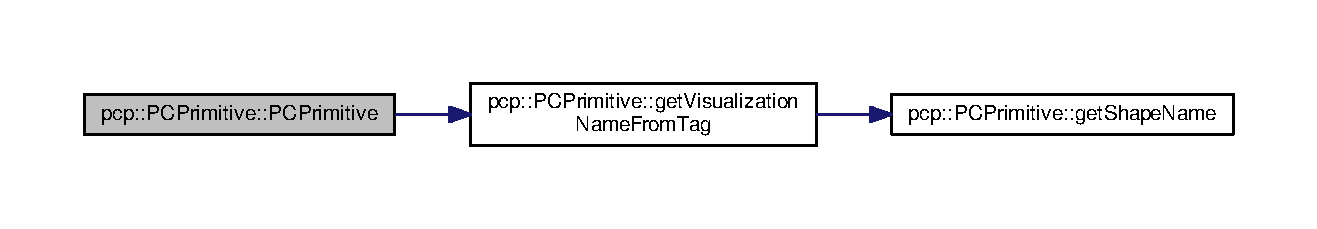
\includegraphics[width=350pt]{classpcp_1_1PCPrimitive_a00c270f938ac1f76c1252422e1f1424f_cgraph}
\end{center}
\end{figure}


\hypertarget{classpcp_1_1PCPrimitive_a3a4da7e50a67144bc1b5b4dfd376b72e}{\index{pcp\-::\-P\-C\-Primitive@{pcp\-::\-P\-C\-Primitive}!$\sim$\-P\-C\-Primitive@{$\sim$\-P\-C\-Primitive}}
\index{$\sim$\-P\-C\-Primitive@{$\sim$\-P\-C\-Primitive}!pcp::PCPrimitive@{pcp\-::\-P\-C\-Primitive}}
\subsubsection[{$\sim$\-P\-C\-Primitive}]{\setlength{\rightskip}{0pt plus 5cm}pcp\-::\-P\-C\-Primitive\-::$\sim$\-P\-C\-Primitive (
\begin{DoxyParamCaption}
{}
\end{DoxyParamCaption}
)\hspace{0.3cm}{\ttfamily [virtual]}}}\label{classpcp_1_1PCPrimitive_a3a4da7e50a67144bc1b5b4dfd376b72e}


Definition at line 26 of file pc\-\_\-primitive.\-cpp.



\subsection{Member Function Documentation}
\hypertarget{classpcp_1_1PCPrimitive_a2d8fe7d2a3a6454cb378bdbbff408cf0}{\index{pcp\-::\-P\-C\-Primitive@{pcp\-::\-P\-C\-Primitive}!copy\-Coefficients@{copy\-Coefficients}}
\index{copy\-Coefficients@{copy\-Coefficients}!pcp::PCPrimitive@{pcp\-::\-P\-C\-Primitive}}
\subsubsection[{copy\-Coefficients}]{\setlength{\rightskip}{0pt plus 5cm}Model\-Coefficients pcp\-::\-P\-C\-Primitive\-::copy\-Coefficients (
\begin{DoxyParamCaption}
\item[{Model\-Coefficients\-::\-Ptr}]{input}
\end{DoxyParamCaption}
)\hspace{0.3cm}{\ttfamily [private]}}}\label{classpcp_1_1PCPrimitive_a2d8fe7d2a3a6454cb378bdbbff408cf0}


Definition at line 64 of file pc\-\_\-primitive.\-cpp.

\hypertarget{classpcp_1_1PCPrimitive_ac774df2f9bb393e9a1491da1b0131d4f}{\index{pcp\-::\-P\-C\-Primitive@{pcp\-::\-P\-C\-Primitive}!get\-Primitive\-Cloud@{get\-Primitive\-Cloud}}
\index{get\-Primitive\-Cloud@{get\-Primitive\-Cloud}!pcp::PCPrimitive@{pcp\-::\-P\-C\-Primitive}}
\subsubsection[{get\-Primitive\-Cloud}]{\setlength{\rightskip}{0pt plus 5cm}{\bf P\-C\-L\-Cloud} pcp\-::\-P\-C\-Primitive\-::get\-Primitive\-Cloud (
\begin{DoxyParamCaption}
{}
\end{DoxyParamCaption}
)}}\label{classpcp_1_1PCPrimitive_ac774df2f9bb393e9a1491da1b0131d4f}


Definition at line 88 of file pc\-\_\-primitive.\-cpp.



References primitive\-Cloud.

\hypertarget{classpcp_1_1PCPrimitive_aafdd30869b5e09e394d70efebe5eac2a}{\index{pcp\-::\-P\-C\-Primitive@{pcp\-::\-P\-C\-Primitive}!get\-Primitive\-Normal@{get\-Primitive\-Normal}}
\index{get\-Primitive\-Normal@{get\-Primitive\-Normal}!pcp::PCPrimitive@{pcp\-::\-P\-C\-Primitive}}
\subsubsection[{get\-Primitive\-Normal}]{\setlength{\rightskip}{0pt plus 5cm}{\bf P\-C\-L\-Normal} pcp\-::\-P\-C\-Primitive\-::get\-Primitive\-Normal (
\begin{DoxyParamCaption}
{}
\end{DoxyParamCaption}
)}}\label{classpcp_1_1PCPrimitive_aafdd30869b5e09e394d70efebe5eac2a}


Definition at line 91 of file pc\-\_\-primitive.\-cpp.



References primitive\-Normals.

\hypertarget{classpcp_1_1PCPrimitive_a1251deb8c39370d0ed5e7d2c7290063f}{\index{pcp\-::\-P\-C\-Primitive@{pcp\-::\-P\-C\-Primitive}!get\-Shape\-Mapidx@{get\-Shape\-Mapidx}}
\index{get\-Shape\-Mapidx@{get\-Shape\-Mapidx}!pcp::PCPrimitive@{pcp\-::\-P\-C\-Primitive}}
\subsubsection[{get\-Shape\-Mapidx}]{\setlength{\rightskip}{0pt plus 5cm}int pcp\-::\-P\-C\-Primitive\-::get\-Shape\-Mapidx (
\begin{DoxyParamCaption}
{}
\end{DoxyParamCaption}
)}}\label{classpcp_1_1PCPrimitive_a1251deb8c39370d0ed5e7d2c7290063f}


Definition at line 82 of file pc\-\_\-primitive.\-cpp.



References shape\-Map\-Idx.

\hypertarget{classpcp_1_1PCPrimitive_a9f507218fd4c442d0daa4938e2e71c10}{\index{pcp\-::\-P\-C\-Primitive@{pcp\-::\-P\-C\-Primitive}!get\-Shape\-Name@{get\-Shape\-Name}}
\index{get\-Shape\-Name@{get\-Shape\-Name}!pcp::PCPrimitive@{pcp\-::\-P\-C\-Primitive}}
\subsubsection[{get\-Shape\-Name}]{\setlength{\rightskip}{0pt plus 5cm}string pcp\-::\-P\-C\-Primitive\-::get\-Shape\-Name (
\begin{DoxyParamCaption}
{}
\end{DoxyParamCaption}
)}}\label{classpcp_1_1PCPrimitive_a9f507218fd4c442d0daa4938e2e71c10}


Definition at line 73 of file pc\-\_\-primitive.\-cpp.



References shape\-Name.



Referenced by get\-Visualization\-Name\-From\-Tag().

\hypertarget{classpcp_1_1PCPrimitive_ad92a83f976c6aac8125c7c8997633f21}{\index{pcp\-::\-P\-C\-Primitive@{pcp\-::\-P\-C\-Primitive}!get\-Visualization\-Flag@{get\-Visualization\-Flag}}
\index{get\-Visualization\-Flag@{get\-Visualization\-Flag}!pcp::PCPrimitive@{pcp\-::\-P\-C\-Primitive}}
\subsubsection[{get\-Visualization\-Flag}]{\setlength{\rightskip}{0pt plus 5cm}bool pcp\-::\-P\-C\-Primitive\-::get\-Visualization\-Flag (
\begin{DoxyParamCaption}
{}
\end{DoxyParamCaption}
)}}\label{classpcp_1_1PCPrimitive_ad92a83f976c6aac8125c7c8997633f21}


Definition at line 79 of file pc\-\_\-primitive.\-cpp.



References visualization\-Flag.

\hypertarget{classpcp_1_1PCPrimitive_ae6a97bc88b8cc7e83476413c73e01aeb}{\index{pcp\-::\-P\-C\-Primitive@{pcp\-::\-P\-C\-Primitive}!get\-Visualization\-Name@{get\-Visualization\-Name}}
\index{get\-Visualization\-Name@{get\-Visualization\-Name}!pcp::PCPrimitive@{pcp\-::\-P\-C\-Primitive}}
\subsubsection[{get\-Visualization\-Name}]{\setlength{\rightskip}{0pt plus 5cm}string pcp\-::\-P\-C\-Primitive\-::get\-Visualization\-Name (
\begin{DoxyParamCaption}
{}
\end{DoxyParamCaption}
)}}\label{classpcp_1_1PCPrimitive_ae6a97bc88b8cc7e83476413c73e01aeb}


Definition at line 76 of file pc\-\_\-primitive.\-cpp.



References visualization\-Name.

\hypertarget{classpcp_1_1PCPrimitive_a0764e20850fd7392f657d1cc43e8ec77}{\index{pcp\-::\-P\-C\-Primitive@{pcp\-::\-P\-C\-Primitive}!get\-Visualization\-Name\-From\-Tag@{get\-Visualization\-Name\-From\-Tag}}
\index{get\-Visualization\-Name\-From\-Tag@{get\-Visualization\-Name\-From\-Tag}!pcp::PCPrimitive@{pcp\-::\-P\-C\-Primitive}}
\subsubsection[{get\-Visualization\-Name\-From\-Tag}]{\setlength{\rightskip}{0pt plus 5cm}string pcp\-::\-P\-C\-Primitive\-::get\-Visualization\-Name\-From\-Tag (
\begin{DoxyParamCaption}
\item[{int}]{idx}
\end{DoxyParamCaption}
)\hspace{0.3cm}{\ttfamily [private]}}}\label{classpcp_1_1PCPrimitive_a0764e20850fd7392f657d1cc43e8ec77}


Definition at line 35 of file pc\-\_\-primitive.\-cpp.



References D\-E\-F\-A\-U\-L\-T\-\_\-\-V\-I\-S\-U\-A\-L\-I\-Z\-A\-T\-I\-O\-N\-\_\-\-N\-A\-M\-E\-\_\-\-S\-E\-P\-A\-R\-A\-T\-O\-R, and get\-Shape\-Name().



Referenced by P\-C\-Primitive().



Here is the call graph for this function\-:
\nopagebreak
\begin{figure}[H]
\begin{center}
\leavevmode
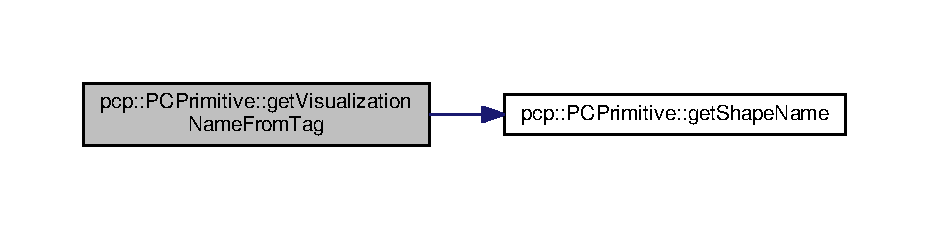
\includegraphics[width=350pt]{classpcp_1_1PCPrimitive_a0764e20850fd7392f657d1cc43e8ec77_cgraph}
\end{center}
\end{figure}




\subsection{Member Data Documentation}
\hypertarget{classpcp_1_1PCPrimitive_ab54a8fb25b750b3808d652f25161ba02}{\index{pcp\-::\-P\-C\-Primitive@{pcp\-::\-P\-C\-Primitive}!D\-E\-F\-A\-U\-L\-T\-\_\-\-S\-H\-A\-P\-E\-\_\-\-N\-A\-M\-E\-\_\-\-C\-L\-U\-S\-T\-E\-R@{D\-E\-F\-A\-U\-L\-T\-\_\-\-S\-H\-A\-P\-E\-\_\-\-N\-A\-M\-E\-\_\-\-C\-L\-U\-S\-T\-E\-R}}
\index{D\-E\-F\-A\-U\-L\-T\-\_\-\-S\-H\-A\-P\-E\-\_\-\-N\-A\-M\-E\-\_\-\-C\-L\-U\-S\-T\-E\-R@{D\-E\-F\-A\-U\-L\-T\-\_\-\-S\-H\-A\-P\-E\-\_\-\-N\-A\-M\-E\-\_\-\-C\-L\-U\-S\-T\-E\-R}!pcp::PCPrimitive@{pcp\-::\-P\-C\-Primitive}}
\subsubsection[{D\-E\-F\-A\-U\-L\-T\-\_\-\-S\-H\-A\-P\-E\-\_\-\-N\-A\-M\-E\-\_\-\-C\-L\-U\-S\-T\-E\-R}]{\setlength{\rightskip}{0pt plus 5cm}const string pcp\-::\-P\-C\-Primitive\-::\-D\-E\-F\-A\-U\-L\-T\-\_\-\-S\-H\-A\-P\-E\-\_\-\-N\-A\-M\-E\-\_\-\-C\-L\-U\-S\-T\-E\-R = \char`\"{}cluster\char`\"{}\hspace{0.3cm}{\ttfamily [static]}}}\label{classpcp_1_1PCPrimitive_ab54a8fb25b750b3808d652f25161ba02}


Definition at line 74 of file pc\-\_\-primitive.\-h.

\hypertarget{classpcp_1_1PCPrimitive_a640bb9e84b55d900e6edbaef8b938d6e}{\index{pcp\-::\-P\-C\-Primitive@{pcp\-::\-P\-C\-Primitive}!D\-E\-F\-A\-U\-L\-T\-\_\-\-S\-H\-A\-P\-E\-\_\-\-N\-A\-M\-E\-\_\-\-P\-L\-A\-N\-E@{D\-E\-F\-A\-U\-L\-T\-\_\-\-S\-H\-A\-P\-E\-\_\-\-N\-A\-M\-E\-\_\-\-P\-L\-A\-N\-E}}
\index{D\-E\-F\-A\-U\-L\-T\-\_\-\-S\-H\-A\-P\-E\-\_\-\-N\-A\-M\-E\-\_\-\-P\-L\-A\-N\-E@{D\-E\-F\-A\-U\-L\-T\-\_\-\-S\-H\-A\-P\-E\-\_\-\-N\-A\-M\-E\-\_\-\-P\-L\-A\-N\-E}!pcp::PCPrimitive@{pcp\-::\-P\-C\-Primitive}}
\subsubsection[{D\-E\-F\-A\-U\-L\-T\-\_\-\-S\-H\-A\-P\-E\-\_\-\-N\-A\-M\-E\-\_\-\-P\-L\-A\-N\-E}]{\setlength{\rightskip}{0pt plus 5cm}const string pcp\-::\-P\-C\-Primitive\-::\-D\-E\-F\-A\-U\-L\-T\-\_\-\-S\-H\-A\-P\-E\-\_\-\-N\-A\-M\-E\-\_\-\-P\-L\-A\-N\-E = \char`\"{}plane\char`\"{}\hspace{0.3cm}{\ttfamily [static]}}}\label{classpcp_1_1PCPrimitive_a640bb9e84b55d900e6edbaef8b938d6e}


Definition at line 73 of file pc\-\_\-primitive.\-h.

\hypertarget{classpcp_1_1PCPrimitive_a9dc28983a955e1f9b1813a15e4260386}{\index{pcp\-::\-P\-C\-Primitive@{pcp\-::\-P\-C\-Primitive}!D\-E\-F\-A\-U\-L\-T\-\_\-\-V\-I\-S\-U\-A\-L\-I\-Z\-A\-T\-I\-O\-N\-\_\-\-N\-A\-M\-E\-\_\-\-S\-E\-P\-A\-R\-A\-T\-O\-R@{D\-E\-F\-A\-U\-L\-T\-\_\-\-V\-I\-S\-U\-A\-L\-I\-Z\-A\-T\-I\-O\-N\-\_\-\-N\-A\-M\-E\-\_\-\-S\-E\-P\-A\-R\-A\-T\-O\-R}}
\index{D\-E\-F\-A\-U\-L\-T\-\_\-\-V\-I\-S\-U\-A\-L\-I\-Z\-A\-T\-I\-O\-N\-\_\-\-N\-A\-M\-E\-\_\-\-S\-E\-P\-A\-R\-A\-T\-O\-R@{D\-E\-F\-A\-U\-L\-T\-\_\-\-V\-I\-S\-U\-A\-L\-I\-Z\-A\-T\-I\-O\-N\-\_\-\-N\-A\-M\-E\-\_\-\-S\-E\-P\-A\-R\-A\-T\-O\-R}!pcp::PCPrimitive@{pcp\-::\-P\-C\-Primitive}}
\subsubsection[{D\-E\-F\-A\-U\-L\-T\-\_\-\-V\-I\-S\-U\-A\-L\-I\-Z\-A\-T\-I\-O\-N\-\_\-\-N\-A\-M\-E\-\_\-\-S\-E\-P\-A\-R\-A\-T\-O\-R}]{\setlength{\rightskip}{0pt plus 5cm}const string pcp\-::\-P\-C\-Primitive\-::\-D\-E\-F\-A\-U\-L\-T\-\_\-\-V\-I\-S\-U\-A\-L\-I\-Z\-A\-T\-I\-O\-N\-\_\-\-N\-A\-M\-E\-\_\-\-S\-E\-P\-A\-R\-A\-T\-O\-R = \char`\"{}-\/\char`\"{}\hspace{0.3cm}{\ttfamily [static]}}}\label{classpcp_1_1PCPrimitive_a9dc28983a955e1f9b1813a15e4260386}


Definition at line 76 of file pc\-\_\-primitive.\-h.



Referenced by get\-Visualization\-Name\-From\-Tag().

\hypertarget{classpcp_1_1PCPrimitive_accdf8a12234519275d4276b6706d4703}{\index{pcp\-::\-P\-C\-Primitive@{pcp\-::\-P\-C\-Primitive}!primitive\-Cloud@{primitive\-Cloud}}
\index{primitive\-Cloud@{primitive\-Cloud}!pcp::PCPrimitive@{pcp\-::\-P\-C\-Primitive}}
\subsubsection[{primitive\-Cloud}]{\setlength{\rightskip}{0pt plus 5cm}{\bf P\-C\-L\-Cloud} pcp\-::\-P\-C\-Primitive\-::primitive\-Cloud\hspace{0.3cm}{\ttfamily [private]}}}\label{classpcp_1_1PCPrimitive_accdf8a12234519275d4276b6706d4703}


Definition at line 37 of file pc\-\_\-primitive.\-h.



Referenced by get\-Primitive\-Cloud(), and P\-C\-Primitive().

\hypertarget{classpcp_1_1PCPrimitive_adb0f70b618dddbff203bccd1fa071782}{\index{pcp\-::\-P\-C\-Primitive@{pcp\-::\-P\-C\-Primitive}!primitive\-Coefficients@{primitive\-Coefficients}}
\index{primitive\-Coefficients@{primitive\-Coefficients}!pcp::PCPrimitive@{pcp\-::\-P\-C\-Primitive}}
\subsubsection[{primitive\-Coefficients}]{\setlength{\rightskip}{0pt plus 5cm}Model\-Coefficients pcp\-::\-P\-C\-Primitive\-::primitive\-Coefficients\hspace{0.3cm}{\ttfamily [private]}}}\label{classpcp_1_1PCPrimitive_adb0f70b618dddbff203bccd1fa071782}


Definition at line 39 of file pc\-\_\-primitive.\-h.

\hypertarget{classpcp_1_1PCPrimitive_a96359fda0d8c70e3b074d97bde90b282}{\index{pcp\-::\-P\-C\-Primitive@{pcp\-::\-P\-C\-Primitive}!primitive\-Normals@{primitive\-Normals}}
\index{primitive\-Normals@{primitive\-Normals}!pcp::PCPrimitive@{pcp\-::\-P\-C\-Primitive}}
\subsubsection[{primitive\-Normals}]{\setlength{\rightskip}{0pt plus 5cm}{\bf P\-C\-L\-Normal} pcp\-::\-P\-C\-Primitive\-::primitive\-Normals\hspace{0.3cm}{\ttfamily [private]}}}\label{classpcp_1_1PCPrimitive_a96359fda0d8c70e3b074d97bde90b282}


Definition at line 38 of file pc\-\_\-primitive.\-h.



Referenced by get\-Primitive\-Normal(), and P\-C\-Primitive().

\hypertarget{classpcp_1_1PCPrimitive_a809c274d155e9b552cf02a0687b7cc11}{\index{pcp\-::\-P\-C\-Primitive@{pcp\-::\-P\-C\-Primitive}!shape\-Map\-Idx@{shape\-Map\-Idx}}
\index{shape\-Map\-Idx@{shape\-Map\-Idx}!pcp::PCPrimitive@{pcp\-::\-P\-C\-Primitive}}
\subsubsection[{shape\-Map\-Idx}]{\setlength{\rightskip}{0pt plus 5cm}int pcp\-::\-P\-C\-Primitive\-::shape\-Map\-Idx\hspace{0.3cm}{\ttfamily [private]}}}\label{classpcp_1_1PCPrimitive_a809c274d155e9b552cf02a0687b7cc11}


Definition at line 34 of file pc\-\_\-primitive.\-h.



Referenced by get\-Shape\-Mapidx(), and P\-C\-Primitive().

\hypertarget{classpcp_1_1PCPrimitive_a120d0dd6120b9fe1af74d698d40adb1c}{\index{pcp\-::\-P\-C\-Primitive@{pcp\-::\-P\-C\-Primitive}!shape\-Name@{shape\-Name}}
\index{shape\-Name@{shape\-Name}!pcp::PCPrimitive@{pcp\-::\-P\-C\-Primitive}}
\subsubsection[{shape\-Name}]{\setlength{\rightskip}{0pt plus 5cm}string pcp\-::\-P\-C\-Primitive\-::shape\-Name\hspace{0.3cm}{\ttfamily [private]}}}\label{classpcp_1_1PCPrimitive_a120d0dd6120b9fe1af74d698d40adb1c}


Definition at line 30 of file pc\-\_\-primitive.\-h.



Referenced by get\-Shape\-Name(), and P\-C\-Primitive().

\hypertarget{classpcp_1_1PCPrimitive_a44cc3f58388966da71e1b07b52d3081c}{\index{pcp\-::\-P\-C\-Primitive@{pcp\-::\-P\-C\-Primitive}!visualization\-Flag@{visualization\-Flag}}
\index{visualization\-Flag@{visualization\-Flag}!pcp::PCPrimitive@{pcp\-::\-P\-C\-Primitive}}
\subsubsection[{visualization\-Flag}]{\setlength{\rightskip}{0pt plus 5cm}bool pcp\-::\-P\-C\-Primitive\-::visualization\-Flag\hspace{0.3cm}{\ttfamily [private]}}}\label{classpcp_1_1PCPrimitive_a44cc3f58388966da71e1b07b52d3081c}


Definition at line 32 of file pc\-\_\-primitive.\-h.



Referenced by get\-Visualization\-Flag(), and P\-C\-Primitive().

\hypertarget{classpcp_1_1PCPrimitive_a8ac9332a85fb342e957959c97012f4d3}{\index{pcp\-::\-P\-C\-Primitive@{pcp\-::\-P\-C\-Primitive}!visualization\-Name@{visualization\-Name}}
\index{visualization\-Name@{visualization\-Name}!pcp::PCPrimitive@{pcp\-::\-P\-C\-Primitive}}
\subsubsection[{visualization\-Name}]{\setlength{\rightskip}{0pt plus 5cm}string pcp\-::\-P\-C\-Primitive\-::visualization\-Name\hspace{0.3cm}{\ttfamily [private]}}}\label{classpcp_1_1PCPrimitive_a8ac9332a85fb342e957959c97012f4d3}


Definition at line 31 of file pc\-\_\-primitive.\-h.



Referenced by get\-Visualization\-Name(), and P\-C\-Primitive().



The documentation for this class was generated from the following files\-:\begin{DoxyCompactItemize}
\item 
src/point\-\_\-cloud\-\_\-library/\hyperlink{pc__primitive_8h}{pc\-\_\-primitive.\-h}\item 
src/point\-\_\-cloud\-\_\-library/\hyperlink{pc__primitive_8cpp}{pc\-\_\-primitive.\-cpp}\end{DoxyCompactItemize}

\hypertarget{structvector3d}{\section{vector3d Struct Reference}
\label{structvector3d}\index{vector3d@{vector3d}}
}
\subsection*{Public Attributes}
\begin{DoxyCompactItemize}
\item 
float \hyperlink{structvector3d_add24ba608397ce7664f51369fc6a1ba4}{x}
\item 
float \hyperlink{structvector3d_a64dec3fa34e765f42a7c716dbc4559d2}{y}
\item 
float \hyperlink{structvector3d_a4e5e948ffcf14e91ebec29e889ced5be}{z}
\end{DoxyCompactItemize}


\subsection{Detailed Description}


Definition at line 34 of file cone\-\_\-segmentation\-\_\-srv.\-cpp.



\subsection{Member Data Documentation}
\hypertarget{structvector3d_add24ba608397ce7664f51369fc6a1ba4}{\index{vector3d@{vector3d}!x@{x}}
\index{x@{x}!vector3d@{vector3d}}
\subsubsection[{x}]{\setlength{\rightskip}{0pt plus 5cm}float vector3d\-::x}}\label{structvector3d_add24ba608397ce7664f51369fc6a1ba4}


Definition at line 35 of file cone\-\_\-segmentation\-\_\-srv.\-cpp.



Referenced by get\-Normalize\-Axes\-Direction\-Vector(), get\-Point\-On\-Axes(), get\-Vector\-Between\-Points(), ransac\-Cone\-Detaction(), and ransac\-Cylinder\-Detaction().

\hypertarget{structvector3d_a64dec3fa34e765f42a7c716dbc4559d2}{\index{vector3d@{vector3d}!y@{y}}
\index{y@{y}!vector3d@{vector3d}}
\subsubsection[{y}]{\setlength{\rightskip}{0pt plus 5cm}float vector3d\-::y}}\label{structvector3d_a64dec3fa34e765f42a7c716dbc4559d2}


Definition at line 36 of file cone\-\_\-segmentation\-\_\-srv.\-cpp.



Referenced by get\-Normalize\-Axes\-Direction\-Vector(), get\-Point\-On\-Axes(), get\-Vector\-Between\-Points(), ransac\-Cone\-Detaction(), and ransac\-Cylinder\-Detaction().

\hypertarget{structvector3d_a4e5e948ffcf14e91ebec29e889ced5be}{\index{vector3d@{vector3d}!z@{z}}
\index{z@{z}!vector3d@{vector3d}}
\subsubsection[{z}]{\setlength{\rightskip}{0pt plus 5cm}float vector3d\-::z}}\label{structvector3d_a4e5e948ffcf14e91ebec29e889ced5be}


Definition at line 37 of file cone\-\_\-segmentation\-\_\-srv.\-cpp.



Referenced by get\-Normalize\-Axes\-Direction\-Vector(), get\-Point\-On\-Axes(), get\-Vector\-Between\-Points(), ransac\-Cone\-Detaction(), and ransac\-Cylinder\-Detaction().



The documentation for this struct was generated from the following files\-:\begin{DoxyCompactItemize}
\item 
src/segmentation\-\_\-services/\hyperlink{cone__segmentation__srv_8cpp}{cone\-\_\-segmentation\-\_\-srv.\-cpp}\item 
src/segmentation\-\_\-services/\hyperlink{cylinder__segmentation__srv_8cpp}{cylinder\-\_\-segmentation\-\_\-srv.\-cpp}\end{DoxyCompactItemize}

\chapter{File Documentation}
\hypertarget{obj__segmentation_8cpp}{\section{src/obj\-\_\-segmentation.cpp File Reference}
\label{obj__segmentation_8cpp}\index{src/obj\-\_\-segmentation.\-cpp@{src/obj\-\_\-segmentation.\-cpp}}
}


The P\-I\-T\-T starting node, to {\bfseries preprocessing} the Point Cloud for primitive identification.  


{\ttfamily \#include $<$pcl\-\_\-ros/point\-\_\-cloud.\-h$>$}\\*
{\ttfamily \#include $<$pcl/common/transforms.\-h$>$}\\*
{\ttfamily \#include $<$tf/transform\-\_\-listener.\-h$>$}\\*
{\ttfamily \#include $<$std\-\_\-msgs/\-Float64.\-h$>$}\\*
{\ttfamily \#include \char`\"{}pitt\-\_\-msgs/\-Deep\-Filter.\-h\char`\"{}}\\*
{\ttfamily \#include \char`\"{}pitt\-\_\-msgs/\-Support\-Segmentation.\-h\char`\"{}}\\*
{\ttfamily \#include \char`\"{}pitt\-\_\-msgs/\-Cluster\-Segmentation.\-h\char`\"{}}\\*
{\ttfamily \#include \char`\"{}pitt\-\_\-msgs/\-Arm\-Filter.\-h\char`\"{}}\\*
{\ttfamily \#include \char`\"{}pitt\-\_\-msgs/\-Clusters\-Output.\-h\char`\"{}}\\*
{\ttfamily \#include \char`\"{}point\-\_\-cloud\-\_\-library/pc\-\_\-manager.\-h\char`\"{}}\\*
{\ttfamily \#include \char`\"{}point\-\_\-cloud\-\_\-library/srv\-\_\-manager.\-h\char`\"{}}\\*
Include dependency graph for obj\-\_\-segmentation.\-cpp\-:\nopagebreak
\begin{figure}[H]
\begin{center}
\leavevmode
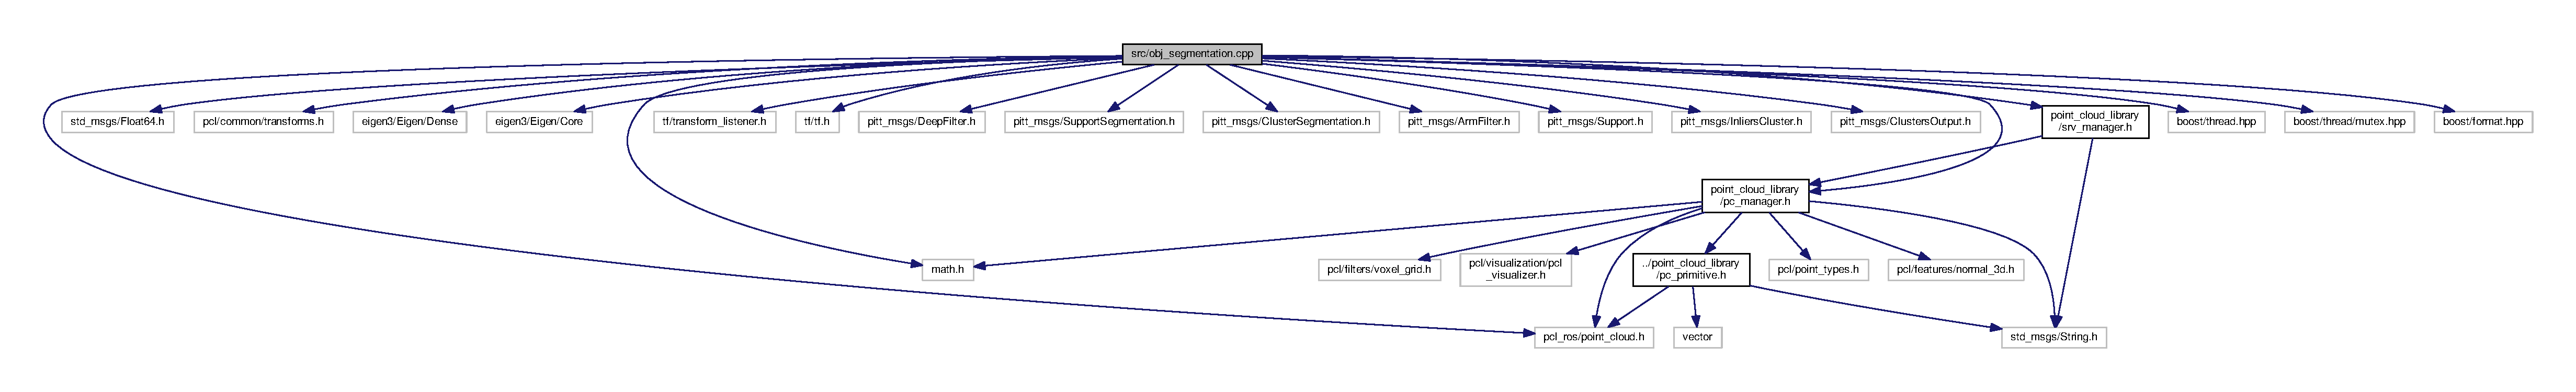
\includegraphics[width=350pt]{obj__segmentation_8cpp__incl}
\end{center}
\end{figure}
\subsection*{Typedefs}
\begin{DoxyCompactItemize}
\item 
typedef vector\\*
$<$ pitt\-\_\-msgs\-::\-Support $>$ \hyperlink{obj__segmentation_8cpp_a54e1c5ec7922766e1a02d8e9b7e3856e}{Inlier\-Supports}
\begin{DoxyCompactList}\small\item\em a vector of costom messages to describe tables. \end{DoxyCompactList}\item 
typedef boost\-::shared\-\_\-ptr\\*
$<$ vector$<$ pitt\-\_\-msgs\-::\-Support $>$ $>$ \hyperlink{obj__segmentation_8cpp_a794c4e0ea8acf9f34c17b066fbf0869d}{Inlier\-Supports\-Ptr}
\begin{DoxyCompactList}\small\item\em a pointer to a \hyperlink{obj__segmentation_8cpp_a54e1c5ec7922766e1a02d8e9b7e3856e}{Inlier\-Supports}. \end{DoxyCompactList}\item 
typedef vector\\*
$<$ pitt\-\_\-msgs\-::\-Inliers\-Cluster $>$ \hyperlink{obj__segmentation_8cpp_a6b657f4959d56c53eaf6be891386bd22}{Inlier\-Clusters}
\begin{DoxyCompactList}\small\item\em a vector of costom messages to describe objects on a table. \end{DoxyCompactList}\item 
typedef boost\-::shared\-\_\-ptr\\*
$<$ vector\\*
$<$ pitt\-\_\-msgs\-::\-Inliers\-Cluster $>$ $>$ \hyperlink{obj__segmentation_8cpp_a50bb89dc3a9b0601f031cbd80235d27e}{Inlier\-Cluster\-Ptr}
\begin{DoxyCompactList}\small\item\em a pointer to a \hyperlink{obj__segmentation_8cpp_a6b657f4959d56c53eaf6be891386bd22}{Inlier\-Clusters}. \end{DoxyCompactList}\end{DoxyCompactItemize}
\subsection*{Functions}
\begin{DoxyCompactItemize}
\item 
void \hyperlink{obj__segmentation_8cpp_aca73ab26cae45b4b998a3cca9e4f75bc}{vis\-Spin} ()
\begin{DoxyCompactList}\small\item\em make the visualisation spinning without lagging acroos multi updating. \end{DoxyCompactList}\item 
bool \hyperlink{obj__segmentation_8cpp_af07806e44f4c8e8e053c64eeee54dca2}{call\-Deep\-Filter} (\hyperlink{pc__primitive_8h_aa14a240c8d999c4f56133c0f70e88783}{P\-C\-L\-Cloud\-Ptr} \&cloud)
\begin{DoxyCompactList}\small\item\em call \hyperlink{deep__filter__srv_8cpp}{deep\-\_\-filter\-\_\-srv.\-cpp} R\-O\-S service. \end{DoxyCompactList}\item 
bool \hyperlink{obj__segmentation_8cpp_a3bba1d36e0ba20c917da78be7258a8ae}{call\-Arm\-Filter} (\hyperlink{pc__primitive_8h_aa14a240c8d999c4f56133c0f70e88783}{P\-C\-L\-Cloud\-Ptr} \&cloud)
\begin{DoxyCompactList}\small\item\em call \hyperlink{arm__filter__srv_8cpp}{arm\-\_\-filter\-\_\-srv.\-cpp} R\-O\-S service. \end{DoxyCompactList}\item 
\hyperlink{obj__segmentation_8cpp_a794c4e0ea8acf9f34c17b066fbf0869d}{Inlier\-Supports\-Ptr} \hyperlink{obj__segmentation_8cpp_a7eb9ce1c694ace5adb8e94f09e54cdae}{call\-Support\-Filter} (\hyperlink{pc__primitive_8h_aa14a240c8d999c4f56133c0f70e88783}{P\-C\-L\-Cloud\-Ptr} \hyperlink{arm__filter__srv_8cpp_a974bd4721d13dc5fa4bd9608eca657db}{input\-Cloud}, \hyperlink{pc__primitive_8h_a1bc38ce8b0c26e5f2d28fae9f3e3ea97}{P\-C\-L\-Normal\-Ptr} normal)
\begin{DoxyCompactList}\small\item\em call support\-\_\-segmentation\-\_\-srv.\-cpp R\-O\-S service. \end{DoxyCompactList}\item 
\hyperlink{obj__segmentation_8cpp_a50bb89dc3a9b0601f031cbd80235d27e}{Inlier\-Cluster\-Ptr} \hyperlink{obj__segmentation_8cpp_a35f42b33ad39e60ed879678fd116fa5b}{call\-Cluster\-Segmentation} (\hyperlink{pc__primitive_8h_aa14a240c8d999c4f56133c0f70e88783}{P\-C\-L\-Cloud\-Ptr} cloud)
\begin{DoxyCompactList}\small\item\em call \hyperlink{cluster__segmentation__srv_8cpp}{cluster\-\_\-segmentation\-\_\-srv.\-cpp} R\-O\-S service. \end{DoxyCompactList}\item 
void \hyperlink{obj__segmentation_8cpp_a480da8a5bc48bba4ac0cd49cfa4e5e7a}{depth\-Acquisition} (const Point\-Cloud2\-Ptr \&input)
\begin{DoxyCompactList}\small\item\em Node callback. \end{DoxyCompactList}\item 
int \hyperlink{obj__segmentation_8cpp_a3c04138a5bfe5d72780bb7e82a18e627}{main} (int argc, char $\ast$$\ast$argv)
\begin{DoxyCompactList}\small\item\em It initialise this R\-O\-S node and spin in order to activate the \hyperlink{obj__segmentation_8cpp_a480da8a5bc48bba4ac0cd49cfa4e5e7a}{depth\-Acquisition} callback as soon as new data is available. It also listens and updates the \hyperlink{obj__segmentation_8cpp_abeb91134d7b10cc7475f7fa946e66a34}{pcl\-Transform} matrix. \end{DoxyCompactList}\end{DoxyCompactItemize}
\subsection*{Variables}
\begin{DoxyCompactItemize}
\item 
static const int \hyperlink{obj__segmentation_8cpp_a3fea3689c92e1b2fcebd3eeafee94a5e}{M\-I\-N\-\_\-\-P\-O\-I\-N\-T\-\_\-\-I\-N\-\_\-\-O\-R\-I\-G\-I\-N\-A\-L\-\_\-\-C\-L\-O\-U\-D} = 30
\begin{DoxyCompactList}\small\item\em the cloud will be not not processed if has less number of points \end{DoxyCompactList}\item 
bool \hyperlink{obj__segmentation_8cpp_ac6f703bc9e7358560334737266db326c}{input\-Show\-Original\-Cloud}
\begin{DoxyCompactList}\small\item\em flag for showing raw cloud (white points) on the visualiser of this node. \end{DoxyCompactList}\item 
bool \hyperlink{obj__segmentation_8cpp_acece8259b4a7b4327562daa817a43ef0}{input\-Show\-Support\-Clouds}
\begin{DoxyCompactList}\small\item\em flag for showing identified tables (brown points) on the visualiser of this node. \end{DoxyCompactList}\item 
bool \hyperlink{obj__segmentation_8cpp_ab64cbde8b32aa3524e9fb94bb4d24525}{input\-Show\-Cluster\-Clouds}
\begin{DoxyCompactList}\small\item\em flag for showing identified objects (random colors) on the visualiser of this node. \end{DoxyCompactList}\item 
bool \hyperlink{obj__segmentation_8cpp_aea198f61928e89fc5332d092619b04f5}{input\-Show\-Object\-On\-Support}
\begin{DoxyCompactList}\small\item\em flag for showing identified all the points on the table (orange points) on the visualiser of this node. \end{DoxyCompactList}\item 
string \hyperlink{obj__segmentation_8cpp_a6317446c893a78108aab89bf69a4b66a}{centroid\-Log\-File\-Path}
\begin{DoxyCompactList}\small\item\em file path to lag the centroids of the acquired objects in a table. Set to empty to do not log on file. \end{DoxyCompactList}\item 
\hyperlink{classpcm_1_1PCManager}{pcm\-::\-P\-C\-Manager} $\ast$ \hyperlink{obj__segmentation_8cpp_a21221f555fa05f2c3f45ff5592a25197}{manager} = new \hyperlink{classpcm_1_1PCManager}{pcm\-::\-P\-C\-Manager}( false)
\begin{DoxyCompactList}\small\item\em variable to initialise the \hyperlink{classpcm_1_1PCManager}{pcm\-::\-P\-C\-Manager}. \end{DoxyCompactList}\item 
ros\-::\-Node\-Handle $\ast$ \hyperlink{obj__segmentation_8cpp_afe3fec681d3658d114dfa8cfff163e82}{nh\-\_\-ptr} = N\-U\-L\-L
\begin{DoxyCompactList}\small\item\em ros handle passed across all services calls. \end{DoxyCompactList}\item 
boost\-::shared\-\_\-ptr\\*
$<$ \hyperlink{pc__manager_8h_a38c805dbc7ad6f06109b85c8e540817a}{visualization\-::\-P\-C\-L\-Visualizer} $>$ \hyperlink{obj__segmentation_8cpp_a6c2d87234fca8dcca11f888098558986}{vis}
\begin{DoxyCompactList}\small\item\em the P\-C\-L visualiser for this node. \end{DoxyCompactList}\item 
ros\-::\-Publisher \hyperlink{obj__segmentation_8cpp_a431711d7fd270977af34b226ed5d5cef}{cluster\-Pub}
\begin{DoxyCompactList}\small\item\em the R\-O\-S publisher in which the message of a new acquistion will be send. \end{DoxyCompactList}\item 
Eigen\-::\-Matrix4f \hyperlink{obj__segmentation_8cpp_abeb91134d7b10cc7475f7fa946e66a34}{pcl\-Transform}
\begin{DoxyCompactList}\small\item\em the transformation matrix between the R\-G\-B-\/\-D sensor and the \hyperlink{namespacesrvm_ac5228e86d6d396c944b11f847746b3b8}{srvm\-::\-P\-A\-R\-A\-M\-\_\-\-N\-A\-M\-E\-\_\-\-I\-N\-P\-U\-T\-\_\-\-C\-L\-O\-U\-D\-\_\-\-R\-E\-F\-E\-R\-E\-N\-C\-E\-\_\-\-F\-R\-A\-M\-E} frame (it can be changed on the fly). \end{DoxyCompactList}\item 
boost\-::thread \hyperlink{obj__segmentation_8cpp_ab83e6219895a4d26706c0d858f8ec288}{vis\-\_\-thread}
\begin{DoxyCompactList}\small\item\em for a better visualiser updating on parallel thread. \end{DoxyCompactList}\item 
boost\-::mutex \hyperlink{obj__segmentation_8cpp_a0dc8882293908d9c8cc15f76a2a49588}{vis\-\_\-mutex}
\begin{DoxyCompactList}\small\item\em for a better visualiser updating during different services calls. \end{DoxyCompactList}\item 
string \hyperlink{obj__segmentation_8cpp_a484374fe771cd860a2ea9f9feda68905}{log\-\_\-str\-\_\-depth} = \char`\"{}Loading...\char`\"{}
\begin{DoxyCompactList}\small\item\em string that will contains info about \hyperlink{deep__filter__srv_8cpp}{deep\-\_\-filter\-\_\-srv.\-cpp} service, shown in the visualiser while the parameters are changed on the fly. \end{DoxyCompactList}\item 
string \hyperlink{obj__segmentation_8cpp_a7024ef4623a4562d025033aa950364f5}{log\-\_\-str\-\_\-supp} = \char`\"{}Loading...\char`\"{}
\begin{DoxyCompactList}\small\item\em string that will contains info about support\-\_\-segmentation\-\_\-srv.\-cpp service, shown in the visualiser while the parameters are changed on the fly. \end{DoxyCompactList}\item 
long \hyperlink{obj__segmentation_8cpp_a848f9977cb150e83cf5464a65dcc9fe4}{scan\-Id} = 0
\begin{DoxyCompactList}\small\item\em so far, it is used only for logging. \end{DoxyCompactList}\end{DoxyCompactItemize}


\subsection{Detailed Description}
The P\-I\-T\-T starting node, to {\bfseries preprocessing} the Point Cloud for primitive identification. {\bfseries File} \par
 ~~~~~~~~~ \hyperlink{obj__segmentation_8cpp}{src/obj\-\_\-segmentation.\-cpp} \begin{DoxyAuthor}{Author}
Buoncompagni Luca, 
\end{DoxyAuthor}
{\bfseries Contacts} \par
 ~~~~~~~~~ \href{mailto:luca.buoncompagni@edu.unige.it}{\tt luca.\-buoncompagni@edu.\-unige.\-it} \begin{DoxyDate}{Date}
May 10, 2015 
\end{DoxyDate}
{\bfseries Institution} \par
 ~~~~~~~~~ D\-I\-B\-R\-I\-S, emaro\-L\-A\-B, University of Genoa. \begin{DoxyVersion}{Version}
2.\-1 

 {\bfseries Programm behaviour} 
\end{DoxyVersion}


~~~~~~~~~ This file implements a R\-O\-S node that acquires Kinect Point Cloud (P\-C) from the topic specified through the\-: \hyperlink{namespacesrvm_afb9bab9dced618a8992cf505cf484b1c}{srvm\-::\-D\-E\-F\-A\-U\-L\-T\-\_\-\-I\-N\-P\-U\-T\-\_\-\-P\-A\-R\-A\-M\-\_\-\-R\-A\-W\-\_\-\-C\-L\-O\-U\-D\-\_\-\-T\-O\-P\-I\-C} parameter (see \hyperlink{obj__segmentation_8cpp_a3c04138a5bfe5d72780bb7e82a18e627}{main} function for more) and performs preprocessing (on \hyperlink{obj__segmentation_8cpp_a480da8a5bc48bba4ac0cd49cfa4e5e7a}{depth\-Acquisition} callback) with the following order\-:
\begin{DoxyEnumerate}
\item P\-C downsampling (see P\-C\-L documentation for more),
\item filtering out far points (see \hyperlink{deep__filter__srv_8cpp}{deep\-\_\-filter\-\_\-srv.\-cpp} R\-O\-S service),
\item filtering out points of robotic arms (see \hyperlink{arm__filter__srv_8cpp}{arm\-\_\-filter\-\_\-srv.\-cpp} R\-O\-S service),
\item P\-C transforming w.\-r.\-t. robot base frame (see T\-F for more),
\item tables segmentation (see \hyperlink{supports__segmentation__srv_8cpp}{supports\-\_\-segmentation\-\_\-srv.\-cpp} R\-O\-S service),
\item objects segmentation, for each support (see \hyperlink{cluster__segmentation__srv_8cpp}{cluster\-\_\-segmentation\-\_\-srv.\-cpp} R\-O\-S service)
\end{DoxyEnumerate}

~~~~~~~~~ The results of this computation (for each table) is published into the topic specified through the \hyperlink{namespacesrvm_a520b8813dc65ba764d59f05a0b316e5c}{srvm\-::\-T\-O\-P\-I\-C\-\_\-\-O\-U\-T\-\_\-\-N\-A\-M\-E\-\_\-\-O\-B\-J\-E\-C\-T\-\_\-\-P\-E\-R\-C\-E\-P\-T\-I\-O\-N} parameter. This topic accommodates an array of 
\begin{DoxyCode}
pitt\_msgs/msg/InlierCluster.msg 
\end{DoxyCode}
 messages (see \href{https://github.com/EmaroLab/pitt_msgs}{\tt pitt\-\_\-msgs} package for more details) that contains, for each recognised object in that table\-:
\begin{DoxyItemize}
\item {\ttfamily sensor\-\_\-msgs/\-Point\-Cloud2} {\ttfamily cloud\-:} ~~ the cloud containing only the object,
\item {\ttfamily int32}\mbox{[}\mbox{]} {\ttfamily inliers\-:} ~~ the index of the points of the object w.\-r.\-t. the original cloud,
\item {\ttfamily float32} {\ttfamily x\-\_\-centroid}, {\ttfamily y\-\_\-centroid}, {\ttfamily z\-\_\-centroid\-:} ~~ the coordinates of the center of mass of the cloud
\item {\ttfamily int32} {\ttfamily shape\-\_\-id\-:} ~~ object identifier. At this stage of the architecture this value is not set (the tracker will do it, see the \href{https://github.com/EmaroLab/pitt_geometric_tracking}{\tt pitt\-\_\-geometric\-\_\-tracking } for an example).
\end{DoxyItemize}

\begin{DoxySeeAlso}{See Also}
\hyperlink{pc__manager_8h}{pc\-\_\-manager.\-h} 

\hyperlink{pc__primitive_8h}{pc\-\_\-primitive.\-h} 

\hyperlink{srv__manager_8h}{srv\-\_\-manager.\-h} 

\hyperlink{ransac__segmentation_8cpp}{ransac\-\_\-segmentation.\-cpp} 

$<$a href="\href{https://github.com/EmaroLab/pitt_geometric_tracking}{\tt https\-://github.\-com/\-Emaro\-Lab/pitt\-\_\-geometric\-\_\-tracking}$>$pitt\-\_\-geometric\-\_\-tracking 
\end{DoxySeeAlso}


Definition in file \hyperlink{obj__segmentation_8cpp_source}{obj\-\_\-segmentation.\-cpp}.



\subsection{Typedef Documentation}
\hypertarget{obj__segmentation_8cpp_a50bb89dc3a9b0601f031cbd80235d27e}{\index{obj\-\_\-segmentation.\-cpp@{obj\-\_\-segmentation.\-cpp}!Inlier\-Cluster\-Ptr@{Inlier\-Cluster\-Ptr}}
\index{Inlier\-Cluster\-Ptr@{Inlier\-Cluster\-Ptr}!obj_segmentation.cpp@{obj\-\_\-segmentation.\-cpp}}
\subsubsection[{Inlier\-Cluster\-Ptr}]{\setlength{\rightskip}{0pt plus 5cm}typedef boost\-::shared\-\_\-ptr$<$ vector$<$ pitt\-\_\-msgs\-::\-Inliers\-Cluster$>$ $>$ {\bf Inlier\-Cluster\-Ptr}}}\label{obj__segmentation_8cpp_a50bb89dc3a9b0601f031cbd80235d27e}


a pointer to a \hyperlink{obj__segmentation_8cpp_a6b657f4959d56c53eaf6be891386bd22}{Inlier\-Clusters}. 

\begin{DoxySeeAlso}{See Also}

\begin{DoxyCode}
pitt\_msgs/msg/InliersCluster.msg 
\end{DoxyCode}
 
\end{DoxySeeAlso}


Definition at line 92 of file obj\-\_\-segmentation.\-cpp.

\hypertarget{obj__segmentation_8cpp_a6b657f4959d56c53eaf6be891386bd22}{\index{obj\-\_\-segmentation.\-cpp@{obj\-\_\-segmentation.\-cpp}!Inlier\-Clusters@{Inlier\-Clusters}}
\index{Inlier\-Clusters@{Inlier\-Clusters}!obj_segmentation.cpp@{obj\-\_\-segmentation.\-cpp}}
\subsubsection[{Inlier\-Clusters}]{\setlength{\rightskip}{0pt plus 5cm}typedef vector$<$ pitt\-\_\-msgs\-::\-Inliers\-Cluster$>$ {\bf Inlier\-Clusters}}}\label{obj__segmentation_8cpp_a6b657f4959d56c53eaf6be891386bd22}


a vector of costom messages to describe objects on a table. 

\begin{DoxySeeAlso}{See Also}

\begin{DoxyCode}
pitt\_msgs/msg/InliersCluster.msg 
\end{DoxyCode}
 
\end{DoxySeeAlso}


Definition at line 87 of file obj\-\_\-segmentation.\-cpp.

\hypertarget{obj__segmentation_8cpp_a54e1c5ec7922766e1a02d8e9b7e3856e}{\index{obj\-\_\-segmentation.\-cpp@{obj\-\_\-segmentation.\-cpp}!Inlier\-Supports@{Inlier\-Supports}}
\index{Inlier\-Supports@{Inlier\-Supports}!obj_segmentation.cpp@{obj\-\_\-segmentation.\-cpp}}
\subsubsection[{Inlier\-Supports}]{\setlength{\rightskip}{0pt plus 5cm}typedef vector$<$ pitt\-\_\-msgs\-::\-Support$>$ {\bf Inlier\-Supports}}}\label{obj__segmentation_8cpp_a54e1c5ec7922766e1a02d8e9b7e3856e}


a vector of costom messages to describe tables. 

\begin{DoxySeeAlso}{See Also}

\begin{DoxyCode}
pitt\_msgs/msg/Support.msg 
\end{DoxyCode}
 
\end{DoxySeeAlso}


Definition at line 77 of file obj\-\_\-segmentation.\-cpp.

\hypertarget{obj__segmentation_8cpp_a794c4e0ea8acf9f34c17b066fbf0869d}{\index{obj\-\_\-segmentation.\-cpp@{obj\-\_\-segmentation.\-cpp}!Inlier\-Supports\-Ptr@{Inlier\-Supports\-Ptr}}
\index{Inlier\-Supports\-Ptr@{Inlier\-Supports\-Ptr}!obj_segmentation.cpp@{obj\-\_\-segmentation.\-cpp}}
\subsubsection[{Inlier\-Supports\-Ptr}]{\setlength{\rightskip}{0pt plus 5cm}typedef boost\-::shared\-\_\-ptr$<$ vector$<$ pitt\-\_\-msgs\-::\-Support$>$ $>$ {\bf Inlier\-Supports\-Ptr}}}\label{obj__segmentation_8cpp_a794c4e0ea8acf9f34c17b066fbf0869d}


a pointer to a \hyperlink{obj__segmentation_8cpp_a54e1c5ec7922766e1a02d8e9b7e3856e}{Inlier\-Supports}. 

\begin{DoxySeeAlso}{See Also}

\begin{DoxyCode}
pitt\_msgs/msg/Support.msg 
\end{DoxyCode}
 
\end{DoxySeeAlso}


Definition at line 82 of file obj\-\_\-segmentation.\-cpp.



\subsection{Function Documentation}
\hypertarget{obj__segmentation_8cpp_a3bba1d36e0ba20c917da78be7258a8ae}{\index{obj\-\_\-segmentation.\-cpp@{obj\-\_\-segmentation.\-cpp}!call\-Arm\-Filter@{call\-Arm\-Filter}}
\index{call\-Arm\-Filter@{call\-Arm\-Filter}!obj_segmentation.cpp@{obj\-\_\-segmentation.\-cpp}}
\subsubsection[{call\-Arm\-Filter}]{\setlength{\rightskip}{0pt plus 5cm}bool call\-Arm\-Filter (
\begin{DoxyParamCaption}
\item[{{\bf P\-C\-L\-Cloud\-Ptr} \&}]{cloud}
\end{DoxyParamCaption}
)}}\label{obj__segmentation_8cpp_a3bba1d36e0ba20c917da78be7258a8ae}


call \hyperlink{arm__filter__srv_8cpp}{arm\-\_\-filter\-\_\-srv.\-cpp} R\-O\-S service. 

It removes, from input parameter, all the points that are belonging to a bounding box around the robot arms.


\begin{DoxyParams}{Parameters}
{\em cloud} & the P\-C from which remove all the points of the arms. \\
\hline
\end{DoxyParams}
\begin{DoxyReturn}{Returns}
false if an error occurs during service call, true otherwise. 
\end{DoxyReturn}
Following, the steeps that this function performs\-:
\begin{DoxyItemize}
\item load the baunding box parameters (default values\-: \hyperlink{namespacesrvm_a78080cf77ae5d29a39ebcd3309b836fc}{srvm\-::\-D\-E\-F\-A\-U\-L\-T\-\_\-\-S\-E\-R\-V\-I\-C\-E\-\_\-\-V\-E\-C\-\_\-\-P\-A\-R\-A\-M\-E\-T\-E\-R\-\_\-\-R\-E\-Q\-U\-E\-S\-T})\-:
\begin{DoxyItemize}
\item \hyperlink{namespacesrvm_a78229888a94a0362b2a4242a212e496f}{srvm\-::\-P\-A\-R\-A\-M\-\_\-\-N\-A\-M\-E\-\_\-\-A\-R\-M\-\_\-\-S\-R\-V\-\_\-\-M\-I\-N\-\_\-\-F\-O\-R\-E\-A\-R\-M\-\_\-\-B\-O\-X},
\item \hyperlink{namespacesrvm_a566bcfbd837fb5450a2c9c6de09d522a}{srvm\-::\-P\-A\-R\-A\-M\-\_\-\-N\-A\-M\-E\-\_\-\-A\-R\-M\-\_\-\-S\-R\-V\-\_\-\-M\-A\-X\-\_\-\-F\-O\-R\-E\-A\-R\-M\-\_\-\-B\-O\-X},
\item \hyperlink{namespacesrvm_ae85ac94c938b94bb075b175237d198b0}{srvm\-::\-P\-A\-R\-A\-M\-\_\-\-N\-A\-M\-E\-\_\-\-A\-R\-M\-\_\-\-S\-R\-V\-\_\-\-M\-I\-N\-\_\-\-E\-L\-B\-O\-W\-\_\-\-B\-O\-X},
\item \hyperlink{namespacesrvm_afeb3197fee2f13444309f3e4ed314392}{srvm\-::\-P\-A\-R\-A\-M\-\_\-\-N\-A\-M\-E\-\_\-\-A\-R\-M\-\_\-\-S\-R\-V\-\_\-\-M\-A\-X\-\_\-\-E\-L\-B\-O\-W\-\_\-\-B\-O\-X},
\end{DoxyItemize}
\item initialise arm filter server,
\item set input data and parameters,
\item call service
\item check for error during service calls.
\item get the repose and overwrite the cloud, if no errors occur. 
\end{DoxyItemize}

Definition at line 251 of file obj\-\_\-segmentation.\-cpp.



References pcm\-::\-P\-C\-Manager\-::cloud\-For\-Ros\-Msg(), pcm\-::\-P\-C\-Manager\-::cloud\-To\-Ros\-Msg(), srvm\-::\-D\-E\-F\-A\-U\-L\-T\-\_\-\-S\-E\-R\-V\-I\-C\-E\-\_\-\-V\-E\-C\-\_\-\-P\-A\-R\-A\-M\-E\-T\-E\-R\-\_\-\-R\-E\-Q\-U\-E\-S\-T(), nh\-\_\-ptr, srvm\-::\-P\-A\-R\-A\-M\-\_\-\-N\-A\-M\-E\-\_\-\-A\-R\-M\-\_\-\-S\-R\-V\-\_\-\-M\-A\-X\-\_\-\-E\-L\-B\-O\-W\-\_\-\-B\-O\-X, srvm\-::\-P\-A\-R\-A\-M\-\_\-\-N\-A\-M\-E\-\_\-\-A\-R\-M\-\_\-\-S\-R\-V\-\_\-\-M\-A\-X\-\_\-\-F\-O\-R\-E\-A\-R\-M\-\_\-\-B\-O\-X, srvm\-::\-P\-A\-R\-A\-M\-\_\-\-N\-A\-M\-E\-\_\-\-A\-R\-M\-\_\-\-S\-R\-V\-\_\-\-M\-I\-N\-\_\-\-E\-L\-B\-O\-W\-\_\-\-B\-O\-X, srvm\-::\-P\-A\-R\-A\-M\-\_\-\-N\-A\-M\-E\-\_\-\-A\-R\-M\-\_\-\-S\-R\-V\-\_\-\-M\-I\-N\-\_\-\-F\-O\-R\-E\-A\-R\-M\-\_\-\-B\-O\-X, and srvm\-::\-S\-R\-V\-\_\-\-N\-A\-M\-E\-\_\-\-A\-R\-M\-\_\-\-F\-I\-L\-T\-E\-R.



Referenced by depth\-Acquisition().



Here is the call graph for this function\-:\nopagebreak
\begin{figure}[H]
\begin{center}
\leavevmode
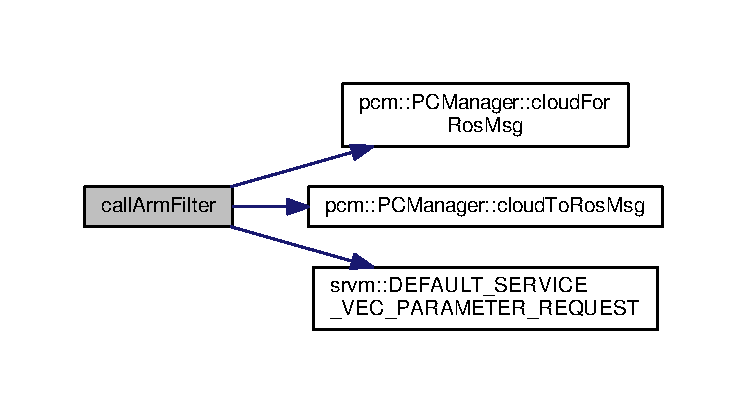
\includegraphics[width=350pt]{obj__segmentation_8cpp_a3bba1d36e0ba20c917da78be7258a8ae_cgraph}
\end{center}
\end{figure}


\hypertarget{obj__segmentation_8cpp_a35f42b33ad39e60ed879678fd116fa5b}{\index{obj\-\_\-segmentation.\-cpp@{obj\-\_\-segmentation.\-cpp}!call\-Cluster\-Segmentation@{call\-Cluster\-Segmentation}}
\index{call\-Cluster\-Segmentation@{call\-Cluster\-Segmentation}!obj_segmentation.cpp@{obj\-\_\-segmentation.\-cpp}}
\subsubsection[{call\-Cluster\-Segmentation}]{\setlength{\rightskip}{0pt plus 5cm}{\bf Inlier\-Cluster\-Ptr} call\-Cluster\-Segmentation (
\begin{DoxyParamCaption}
\item[{{\bf P\-C\-L\-Cloud\-Ptr}}]{cloud}
\end{DoxyParamCaption}
)}}\label{obj__segmentation_8cpp_a35f42b33ad39e60ed879678fd116fa5b}


call \hyperlink{cluster__segmentation__srv_8cpp}{cluster\-\_\-segmentation\-\_\-srv.\-cpp} R\-O\-S service. 

It segments a P\-C in smaller structure where each of them represents a separated object. The points are also described in terms of index in the original cloud.


\begin{DoxyParams}{Parameters}
{\em cloud} & the P\-C to be segmented in clusters. \\
\hline
\end{DoxyParams}
\begin{DoxyReturn}{Returns}
an array of structures that describes separated objects in the cloud. An empty array if errors occur on service call. 
\end{DoxyReturn}
Following, the steeps that this function performs\-:
\begin{DoxyItemize}
\item load the parameters for the server (default values\-: \hyperlink{namespacesrvm_a27b2693a98ba8791767e3c8bebdab105}{srvm\-::\-D\-E\-F\-A\-U\-L\-T\-\_\-\-S\-E\-R\-V\-I\-C\-E\-\_\-\-P\-A\-R\-A\-M\-E\-T\-E\-R\-\_\-\-R\-E\-Q\-U\-E\-S\-T} or \hyperlink{namespacesrvm_a5a9ae08c1a139bbf76b39c5d34f90e2a}{srvm\-::\-D\-E\-F\-A\-U\-L\-T\-\_\-\-S\-E\-R\-V\-I\-C\-E\-\_\-\-P\-A\-R\-A\-M\-E\-T\-E\-R\-\_\-\-R\-E\-Q\-U\-E\-S\-T\-\_\-\-F})\-:
\begin{DoxyItemize}
\item \hyperlink{namespacesrvm_a606c20312640e9cc8710e4d43f0cb167}{srvm\-::\-P\-A\-R\-A\-M\-\_\-\-N\-A\-M\-E\-\_\-\-C\-L\-U\-S\-T\-E\-R\-\_\-\-T\-O\-L\-E\-R\-A\-N\-C\-E},
\item \hyperlink{namespacesrvm_a68216326c13293ff70084f03bb4efa98}{srvm\-::\-P\-A\-R\-A\-M\-\_\-\-N\-A\-M\-E\-\_\-\-C\-L\-U\-S\-T\-E\-R\-\_\-\-M\-I\-N\-\_\-\-R\-A\-T\-E},
\item \hyperlink{namespacesrvm_ac57a3b8f3addc024383db76f1d2c55da}{srvm\-::\-P\-A\-R\-A\-M\-\_\-\-N\-A\-M\-E\-\_\-\-C\-L\-U\-S\-T\-E\-R\-\_\-\-M\-A\-X\-\_\-\-R\-A\-T\-E},
\item \hyperlink{namespacesrvm_a606c20312640e9cc8710e4d43f0cb167}{srvm\-::\-P\-A\-R\-A\-M\-\_\-\-N\-A\-M\-E\-\_\-\-C\-L\-U\-S\-T\-E\-R\-\_\-\-T\-O\-L\-E\-R\-A\-N\-C\-E},
\end{DoxyItemize}
\item initialise claster segmentation server,
\item set input data and parameters,
\item call service,
\item check and log for errors,
\item get the service responce to be returned. 
\end{DoxyItemize}

Definition at line 387 of file obj\-\_\-segmentation.\-cpp.



References pcm\-::\-P\-C\-Manager\-::cloud\-To\-Ros\-Msg(), srvm\-::\-D\-E\-F\-A\-U\-L\-T\-\_\-\-S\-E\-R\-V\-I\-C\-E\-\_\-\-P\-A\-R\-A\-M\-E\-T\-E\-R\-\_\-\-R\-E\-Q\-U\-E\-S\-T, srvm\-::\-D\-E\-F\-A\-U\-L\-T\-\_\-\-S\-E\-R\-V\-I\-C\-E\-\_\-\-P\-A\-R\-A\-M\-E\-T\-E\-R\-\_\-\-R\-E\-Q\-U\-E\-S\-T\-\_\-\-F, nh\-\_\-ptr, srvm\-::\-P\-A\-R\-A\-M\-\_\-\-N\-A\-M\-E\-\_\-\-C\-L\-U\-S\-T\-E\-R\-\_\-\-M\-A\-X\-\_\-\-R\-A\-T\-E, srvm\-::\-P\-A\-R\-A\-M\-\_\-\-N\-A\-M\-E\-\_\-\-C\-L\-U\-S\-T\-E\-R\-\_\-\-M\-I\-N\-\_\-\-R\-A\-T\-E, srvm\-::\-P\-A\-R\-A\-M\-\_\-\-N\-A\-M\-E\-\_\-\-C\-L\-U\-S\-T\-E\-R\-\_\-\-T\-O\-L\-E\-R\-A\-N\-C\-E, and srvm\-::\-S\-R\-V\-\_\-\-N\-A\-M\-E\-\_\-\-C\-U\-S\-T\-E\-R\-\_\-\-F\-I\-L\-T\-E\-R.



Referenced by depth\-Acquisition().



Here is the call graph for this function\-:\nopagebreak
\begin{figure}[H]
\begin{center}
\leavevmode
\includegraphics[width=350pt]{obj__segmentation_8cpp_a35f42b33ad39e60ed879678fd116fa5b_cgraph}
\end{center}
\end{figure}


\hypertarget{obj__segmentation_8cpp_af07806e44f4c8e8e053c64eeee54dca2}{\index{obj\-\_\-segmentation.\-cpp@{obj\-\_\-segmentation.\-cpp}!call\-Deep\-Filter@{call\-Deep\-Filter}}
\index{call\-Deep\-Filter@{call\-Deep\-Filter}!obj_segmentation.cpp@{obj\-\_\-segmentation.\-cpp}}
\subsubsection[{call\-Deep\-Filter}]{\setlength{\rightskip}{0pt plus 5cm}bool call\-Deep\-Filter (
\begin{DoxyParamCaption}
\item[{{\bf P\-C\-L\-Cloud\-Ptr} \&}]{cloud}
\end{DoxyParamCaption}
)}}\label{obj__segmentation_8cpp_af07806e44f4c8e8e053c64eeee54dca2}


call \hyperlink{deep__filter__srv_8cpp}{deep\-\_\-filter\-\_\-srv.\-cpp} R\-O\-S service. 

It removes, from input parameter, all the points further than a threshold on the z-\/axis of the cloud.


\begin{DoxyParams}{Parameters}
{\em cloud} & the P\-C from which remove all the points further than a threshold. \\
\hline
\end{DoxyParams}
\begin{DoxyReturn}{Returns}
false if an error occurs during service call, true otherwise. 
\end{DoxyReturn}
Following, the steeps that this function performs\-:
\begin{DoxyItemize}
\item load the threshold parameter\-: \hyperlink{namespacesrvm_af5f0c98fe811a1ad130ec625e9b2cf75}{srvm\-::\-P\-A\-R\-A\-M\-\_\-\-N\-A\-M\-E\-\_\-\-D\-E\-E\-P\-\_\-\-S\-R\-V\-\_\-\-Z\-\_\-\-T\-H\-R\-E\-S\-H\-O\-L\-D} from R\-O\-S pull. Use \hyperlink{namespacesrvm_a5a9ae08c1a139bbf76b39c5d34f90e2a}{srvm\-::\-D\-E\-F\-A\-U\-L\-T\-\_\-\-S\-E\-R\-V\-I\-C\-E\-\_\-\-P\-A\-R\-A\-M\-E\-T\-E\-R\-\_\-\-R\-E\-Q\-U\-E\-S\-T\-\_\-\-F} as default value,
\item update visualiser texts about the deep threshold value,
\item initialise deep filter server,
\item set input data and parameters,
\item call service,
\item check for error during service calls.
\item get the repose and overwrite the cloud, if no errors occur. 
\end{DoxyItemize}

Definition at line 207 of file obj\-\_\-segmentation.\-cpp.



References pcm\-::\-P\-C\-Manager\-::cloud\-For\-Ros\-Msg(), pcm\-::\-P\-C\-Manager\-::cloud\-To\-Ros\-Msg(), srvm\-::\-D\-E\-F\-A\-U\-L\-T\-\_\-\-S\-E\-R\-V\-I\-C\-E\-\_\-\-P\-A\-R\-A\-M\-E\-T\-E\-R\-\_\-\-R\-E\-Q\-U\-E\-S\-T\-\_\-\-F, input\-Show\-Cluster\-Clouds, input\-Show\-Object\-On\-Support, input\-Show\-Original\-Cloud, input\-Show\-Support\-Clouds, log\-\_\-str\-\_\-depth, nh\-\_\-ptr, srvm\-::\-P\-A\-R\-A\-M\-\_\-\-N\-A\-M\-E\-\_\-\-D\-E\-E\-P\-\_\-\-S\-R\-V\-\_\-\-Z\-\_\-\-T\-H\-R\-E\-S\-H\-O\-L\-D, srvm\-::\-S\-R\-V\-\_\-\-N\-A\-M\-E\-\_\-\-D\-E\-E\-P\-\_\-\-F\-I\-L\-T\-E\-R, vis, and vis\-\_\-mutex.



Referenced by depth\-Acquisition().



Here is the call graph for this function\-:\nopagebreak
\begin{figure}[H]
\begin{center}
\leavevmode
\includegraphics[width=350pt]{obj__segmentation_8cpp_af07806e44f4c8e8e053c64eeee54dca2_cgraph}
\end{center}
\end{figure}


\hypertarget{obj__segmentation_8cpp_a7eb9ce1c694ace5adb8e94f09e54cdae}{\index{obj\-\_\-segmentation.\-cpp@{obj\-\_\-segmentation.\-cpp}!call\-Support\-Filter@{call\-Support\-Filter}}
\index{call\-Support\-Filter@{call\-Support\-Filter}!obj_segmentation.cpp@{obj\-\_\-segmentation.\-cpp}}
\subsubsection[{call\-Support\-Filter}]{\setlength{\rightskip}{0pt plus 5cm}{\bf Inlier\-Supports\-Ptr} call\-Support\-Filter (
\begin{DoxyParamCaption}
\item[{{\bf P\-C\-L\-Cloud\-Ptr}}]{input\-Cloud, }
\item[{{\bf P\-C\-L\-Normal\-Ptr}}]{normal}
\end{DoxyParamCaption}
)}}\label{obj__segmentation_8cpp_a7eb9ce1c694ace5adb8e94f09e54cdae}


call support\-\_\-segmentation\-\_\-srv.\-cpp R\-O\-S service. 

It detects all the vertical planes in the scene and returns the index of their point w.\-r.\-t. to original cloud.


\begin{DoxyParams}{Parameters}
{\em input\-Cloud} & the P\-C from which retrieve the supports. \\
\hline
{\em normal} & the Nolrmal vector of the points of the above cloud. \\
\hline
\end{DoxyParams}
\begin{DoxyReturn}{Returns}
a vector of set of index indicating the points of a support w.\-r.\-t. to acquired cloud. It returns an empty array if errors occur during service call. 
\end{DoxyReturn}
Following, the steeps that this function performs\-:
\begin{DoxyItemize}
\item load the parameters for the server (default values\-: \hyperlink{namespacesrvm_a27b2693a98ba8791767e3c8bebdab105}{srvm\-::\-D\-E\-F\-A\-U\-L\-T\-\_\-\-S\-E\-R\-V\-I\-C\-E\-\_\-\-P\-A\-R\-A\-M\-E\-T\-E\-R\-\_\-\-R\-E\-Q\-U\-E\-S\-T} or \hyperlink{namespacesrvm_a5a9ae08c1a139bbf76b39c5d34f90e2a}{srvm\-::\-D\-E\-F\-A\-U\-L\-T\-\_\-\-S\-E\-R\-V\-I\-C\-E\-\_\-\-P\-A\-R\-A\-M\-E\-T\-E\-R\-\_\-\-R\-E\-Q\-U\-E\-S\-T\-\_\-\-F})\-:
\begin{DoxyItemize}
\item \hyperlink{namespacesrvm_ac6d56e59d27ae79b392d58c0b57d03e1}{srvm\-::\-P\-A\-R\-A\-M\-\_\-\-N\-A\-M\-E\-\_\-\-M\-I\-N\-\_\-\-I\-T\-E\-R\-A\-T\-I\-V\-E\-\_\-\-C\-L\-O\-U\-D\-\_\-\-P\-E\-R\-C\-E\-N\-T\-A\-G\-E},
\item \hyperlink{namespacesrvm_a209e7ad2de58ec5193770fc4d9cd98ab}{srvm\-::\-P\-A\-R\-A\-M\-\_\-\-N\-A\-M\-E\-\_\-\-M\-I\-N\-\_\-\-I\-T\-E\-R\-A\-T\-I\-V\-E\-\_\-\-S\-U\-P\-P\-O\-R\-T\-\_\-\-P\-E\-R\-C\-E\-N\-T\-A\-G\-E},
\item \hyperlink{namespacesrvm_adb071b5e180a1109af154bd4241a250e}{srvm\-::\-P\-A\-R\-A\-M\-\_\-\-N\-A\-M\-E\-\_\-\-H\-O\-R\-I\-Z\-O\-N\-T\-A\-L\-\_\-\-V\-A\-R\-I\-A\-N\-C\-E\-\_\-\-T\-H\-R\-E\-S\-H\-O\-L\-D},
\item \hyperlink{namespacesrvm_af1a83a2964c2f60f7f497f05ef454cfd}{srvm\-::\-P\-A\-R\-A\-M\-\_\-\-N\-A\-M\-E\-\_\-\-R\-A\-N\-S\-A\-C\-\_\-\-I\-N\-\_\-\-S\-H\-A\-P\-E\-\_\-\-D\-I\-S\-T\-A\-N\-C\-E\-\_\-\-P\-O\-I\-N\-T\-\_\-\-T\-H\-R\-E\-S\-H\-O\-L\-D},
\item \hyperlink{namespacesrvm_ad592efae9026788849614a69053f3914}{srvm\-::\-P\-A\-R\-A\-M\-\_\-\-N\-A\-M\-E\-\_\-\-R\-A\-N\-S\-A\-C\-\_\-\-M\-O\-D\-E\-L\-\_\-\-N\-O\-R\-M\-A\-L\-\_\-\-D\-I\-S\-T\-A\-N\-C\-E\-\_\-\-W\-E\-I\-G\-H\-T},
\item \hyperlink{namespacesrvm_aa6b5f05b01cb661c1481c0f40bd916e4}{srvm\-::\-P\-A\-R\-A\-M\-\_\-\-N\-A\-M\-E\-\_\-\-R\-A\-N\-S\-A\-C\-\_\-\-M\-A\-X\-\_\-\-I\-T\-E\-R\-A\-T\-I\-O\-N\-\_\-\-T\-H\-R\-E\-S\-H\-O\-L\-D},
\item \hyperlink{namespacesrvm_a2957bf6ee16944664364c470f1beb958}{srvm\-::\-P\-A\-R\-A\-M\-\_\-\-N\-A\-M\-E\-\_\-\-H\-O\-R\-I\-Z\-O\-N\-T\-A\-L\-\_\-\-A\-X\-I\-S},
\item \hyperlink{namespacesrvm_a07211b3f36f93931af6e67097b75f145}{srvm\-::\-P\-A\-R\-A\-M\-\_\-\-N\-A\-M\-E\-\_\-\-S\-U\-P\-P\-O\-R\-T\-\_\-\-E\-D\-G\-E\-\_\-\-R\-E\-M\-O\-V\-E\-\_\-\-O\-F\-F\-S\-E\-T},
\end{DoxyItemize}
\item initialise support segmentation server,
\item set input data and parameters,
\item call service,
\item check and log for errors,
\item get the service responce to be returned,
\item update the visualiser texts. 
\end{DoxyItemize}

Definition at line 299 of file obj\-\_\-segmentation.\-cpp.



References pcm\-::\-P\-C\-Manager\-::cloud\-To\-Ros\-Msg(), srvm\-::\-D\-E\-F\-A\-U\-L\-T\-\_\-\-S\-E\-R\-V\-I\-C\-E\-\_\-\-P\-A\-R\-A\-M\-E\-T\-E\-R\-\_\-\-R\-E\-Q\-U\-E\-S\-T, srvm\-::\-D\-E\-F\-A\-U\-L\-T\-\_\-\-S\-E\-R\-V\-I\-C\-E\-\_\-\-P\-A\-R\-A\-M\-E\-T\-E\-R\-\_\-\-R\-E\-Q\-U\-E\-S\-T\-\_\-\-F, srvm\-::\-D\-E\-F\-A\-U\-L\-T\-\_\-\-S\-E\-R\-V\-I\-C\-E\-\_\-\-V\-E\-C\-\_\-\-P\-A\-R\-A\-M\-E\-T\-E\-R\-\_\-\-R\-E\-Q\-U\-E\-S\-T(), horizontal\-Axis, input\-Show\-Cluster\-Clouds, input\-Show\-Object\-On\-Support, input\-Show\-Original\-Cloud, input\-Show\-Support\-Clouds, log\-\_\-str\-\_\-supp, nh\-\_\-ptr, pcm\-::\-P\-C\-Manager\-::norm\-To\-Ros\-Msg(), srvm\-::\-P\-A\-R\-A\-M\-\_\-\-N\-A\-M\-E\-\_\-\-H\-O\-R\-I\-Z\-O\-N\-T\-A\-L\-\_\-\-A\-X\-I\-S, srvm\-::\-P\-A\-R\-A\-M\-\_\-\-N\-A\-M\-E\-\_\-\-H\-O\-R\-I\-Z\-O\-N\-T\-A\-L\-\_\-\-V\-A\-R\-I\-A\-N\-C\-E\-\_\-\-T\-H\-R\-E\-S\-H\-O\-L\-D, srvm\-::\-P\-A\-R\-A\-M\-\_\-\-N\-A\-M\-E\-\_\-\-M\-I\-N\-\_\-\-I\-T\-E\-R\-A\-T\-I\-V\-E\-\_\-\-C\-L\-O\-U\-D\-\_\-\-P\-E\-R\-C\-E\-N\-T\-A\-G\-E, srvm\-::\-P\-A\-R\-A\-M\-\_\-\-N\-A\-M\-E\-\_\-\-M\-I\-N\-\_\-\-I\-T\-E\-R\-A\-T\-I\-V\-E\-\_\-\-S\-U\-P\-P\-O\-R\-T\-\_\-\-P\-E\-R\-C\-E\-N\-T\-A\-G\-E, srvm\-::\-P\-A\-R\-A\-M\-\_\-\-N\-A\-M\-E\-\_\-\-R\-A\-N\-S\-A\-C\-\_\-\-I\-N\-\_\-\-S\-H\-A\-P\-E\-\_\-\-D\-I\-S\-T\-A\-N\-C\-E\-\_\-\-P\-O\-I\-N\-T\-\_\-\-T\-H\-R\-E\-S\-H\-O\-L\-D, srvm\-::\-P\-A\-R\-A\-M\-\_\-\-N\-A\-M\-E\-\_\-\-R\-A\-N\-S\-A\-C\-\_\-\-M\-A\-X\-\_\-\-I\-T\-E\-R\-A\-T\-I\-O\-N\-\_\-\-T\-H\-R\-E\-S\-H\-O\-L\-D, srvm\-::\-P\-A\-R\-A\-M\-\_\-\-N\-A\-M\-E\-\_\-\-R\-A\-N\-S\-A\-C\-\_\-\-M\-O\-D\-E\-L\-\_\-\-N\-O\-R\-M\-A\-L\-\_\-\-D\-I\-S\-T\-A\-N\-C\-E\-\_\-\-W\-E\-I\-G\-H\-T, srvm\-::\-P\-A\-R\-A\-M\-\_\-\-N\-A\-M\-E\-\_\-\-S\-U\-P\-P\-O\-R\-T\-\_\-\-E\-D\-G\-E\-\_\-\-R\-E\-M\-O\-V\-E\-\_\-\-O\-F\-F\-S\-E\-T, ransac\-Max\-Iteration, srvm\-::\-S\-R\-V\-\_\-\-N\-A\-M\-E\-\_\-\-S\-U\-P\-P\-O\-R\-T\-\_\-\-F\-I\-L\-T\-E\-R, vis, and vis\-\_\-mutex.



Referenced by depth\-Acquisition().



Here is the call graph for this function\-:\nopagebreak
\begin{figure}[H]
\begin{center}
\leavevmode
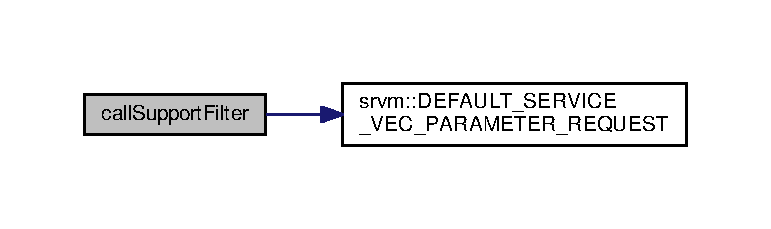
\includegraphics[width=350pt]{obj__segmentation_8cpp_a7eb9ce1c694ace5adb8e94f09e54cdae_cgraph}
\end{center}
\end{figure}


\hypertarget{obj__segmentation_8cpp_a480da8a5bc48bba4ac0cd49cfa4e5e7a}{\index{obj\-\_\-segmentation.\-cpp@{obj\-\_\-segmentation.\-cpp}!depth\-Acquisition@{depth\-Acquisition}}
\index{depth\-Acquisition@{depth\-Acquisition}!obj_segmentation.cpp@{obj\-\_\-segmentation.\-cpp}}
\subsubsection[{depth\-Acquisition}]{\setlength{\rightskip}{0pt plus 5cm}void depth\-Acquisition (
\begin{DoxyParamCaption}
\item[{const Point\-Cloud2\-Ptr \&}]{input}
\end{DoxyParamCaption}
)}}\label{obj__segmentation_8cpp_a480da8a5bc48bba4ac0cd49cfa4e5e7a}


Node callback. 

It is called as soon as a new P\-C acquisition is available from the sensor. It processes the clud based on R\-O\-S services\-:
\begin{DoxyEnumerate}
\item \hyperlink{deep__filter__srv_8cpp}{deep\-\_\-filter\-\_\-srv.\-cpp}
\item \hyperlink{arm__filter__srv_8cpp}{arm\-\_\-filter\-\_\-srv.\-cpp}
\item \hyperlink{supports__segmentation__srv_8cpp}{supports\-\_\-segmentation\-\_\-srv.\-cpp}
\item \hyperlink{cluster__segmentation__srv_8cpp}{cluster\-\_\-segmentation\-\_\-srv.\-cpp}
\end{DoxyEnumerate}

and publishes the output message if a successfully acquisition occurs.


\begin{DoxyParams}{Parameters}
{\em input} & the Point Cloud message published on the input topic. \\
\hline
\end{DoxyParams}
\begin{DoxySeeAlso}{See Also}
\hyperlink{obj__segmentation_8cpp_a3c04138a5bfe5d72780bb7e82a18e627}{main} 

\hyperlink{obj__segmentation_8cpp_af07806e44f4c8e8e053c64eeee54dca2}{call\-Deep\-Filter} 

\hyperlink{obj__segmentation_8cpp_a3bba1d36e0ba20c917da78be7258a8ae}{call\-Arm\-Filter} 

\hyperlink{obj__segmentation_8cpp_a7eb9ce1c694ace5adb8e94f09e54cdae}{call\-Support\-Filter} 

\hyperlink{obj__segmentation_8cpp_a35f42b33ad39e60ed879678fd116fa5b}{call\-Cluster\-Segmentation} 
\end{DoxySeeAlso}
Following, the steeps that this function performs\-:


\begin{DoxyItemize}
\item get Kinect P\-C inputs as a standard pcl cloud,
\item compute down-\/sampling (\hyperlink{classpcm_1_1PCManager_ab9c66b0834ca1ef0c1c01e21400103dd}{pcm\-::\-P\-C\-Manager\-::down\-Sampling}),
\item call deep filter server (\hyperlink{obj__segmentation_8cpp_af07806e44f4c8e8e053c64eeee54dca2}{call\-Deep\-Filter}),
\item if success\-: call arm filter server (\hyperlink{obj__segmentation_8cpp_a3bba1d36e0ba20c917da78be7258a8ae}{call\-Arm\-Filter}),
\item if success\-: transform the cloud w.\-r.\-t. \hyperlink{obj__segmentation_8cpp_abeb91134d7b10cc7475f7fa946e66a34}{pcl\-Transform},
\item stop if too few points are remaining (w.\-r.\-t. \hyperlink{obj__segmentation_8cpp_a3fea3689c92e1b2fcebd3eeafee94a5e}{M\-I\-N\-\_\-\-P\-O\-I\-N\-T\-\_\-\-I\-N\-\_\-\-O\-R\-I\-G\-I\-N\-A\-L\-\_\-\-C\-L\-O\-U\-D}). Otherwise ...
\item compute the normals off all the points,
\item show original cloud as gray points, if \hyperlink{obj__segmentation_8cpp_ac6f703bc9e7358560334737266db326c}{input\-Show\-Original\-Cloud} is true,
\item call the support segmentation service (\hyperlink{obj__segmentation_8cpp_a7eb9ce1c694ace5adb8e94f09e54cdae}{call\-Support\-Filter}),
\item for all the detected supports ...
\item show supports as brown points, if \hyperlink{obj__segmentation_8cpp_acece8259b4a7b4327562daa817a43ef0}{input\-Show\-Support\-Clouds} is true,
\item show cloud of the object on the horizontal plane, as orange points, if \hyperlink{obj__segmentation_8cpp_aea198f61928e89fc5332d092619b04f5}{input\-Show\-Object\-On\-Support} is true,
\item call cluster segmentation service (\hyperlink{obj__segmentation_8cpp_a35f42b33ad39e60ed879678fd116fa5b}{call\-Cluster\-Segmentation}),
\item if there is at least one cluster, prepare node output message containing all the claster information for a support,
\item show cloud of the segmented objects, with random colors, if \hyperlink{obj__segmentation_8cpp_ab64cbde8b32aa3524e9fb94bb4d24525}{input\-Show\-Cluster\-Clouds} is true,
\item prepare detached clusters center of mass for logging,
\item publish the center of mass of the detached clusters for a specific support,
\item print on screen the results,
\item if \hyperlink{obj__segmentation_8cpp_a6317446c893a78108aab89bf69a4b66a}{centroid\-Log\-File\-Path} is not empty, print the same results on file. 
\end{DoxyItemize}

Definition at line 451 of file obj\-\_\-segmentation.\-cpp.



References call\-Arm\-Filter(), call\-Cluster\-Segmentation(), call\-Deep\-Filter(), call\-Support\-Filter(), centroid\-File\-Log, centroid\-Log\-File\-Path, pcm\-::\-P\-C\-Manager\-::cloud\-For\-Ros\-Msg(), cluster\-Pub, pcm\-::\-P\-C\-Manager\-::down\-Sampling(), pcm\-::\-P\-C\-Manager\-::estimate\-Normal(), input\-Show\-Cluster\-Clouds, input\-Show\-Object\-On\-Support, input\-Show\-Original\-Cloud, input\-Show\-Support\-Clouds, M\-I\-N\-\_\-\-P\-O\-I\-N\-T\-\_\-\-I\-N\-\_\-\-O\-R\-I\-G\-I\-N\-A\-L\-\_\-\-C\-L\-O\-U\-D, pcl\-Transform, scan\-Id, pcm\-::\-P\-C\-Manager\-::update\-Visor(), vis, vis\-\_\-mutex, and pcm\-::\-P\-C\-Manager\-::write\-To\-File().



Referenced by main().



Here is the call graph for this function\-:\nopagebreak
\begin{figure}[H]
\begin{center}
\leavevmode
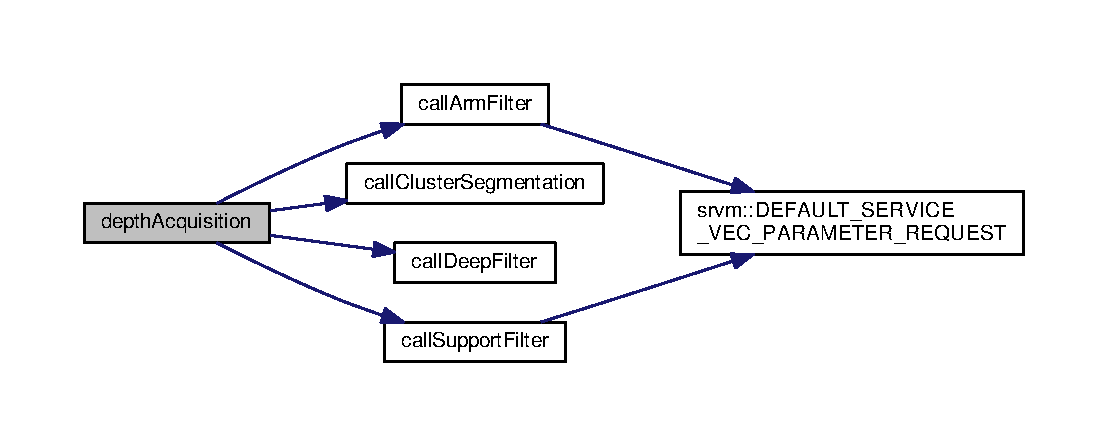
\includegraphics[width=350pt]{obj__segmentation_8cpp_a480da8a5bc48bba4ac0cd49cfa4e5e7a_cgraph}
\end{center}
\end{figure}


\hypertarget{obj__segmentation_8cpp_a3c04138a5bfe5d72780bb7e82a18e627}{\index{obj\-\_\-segmentation.\-cpp@{obj\-\_\-segmentation.\-cpp}!main@{main}}
\index{main@{main}!obj_segmentation.cpp@{obj\-\_\-segmentation.\-cpp}}
\subsubsection[{main}]{\setlength{\rightskip}{0pt plus 5cm}int main (
\begin{DoxyParamCaption}
\item[{int}]{argc, }
\item[{char $\ast$$\ast$}]{argv}
\end{DoxyParamCaption}
)}}\label{obj__segmentation_8cpp_a3c04138a5bfe5d72780bb7e82a18e627}


It initialise this R\-O\-S node and spin in order to activate the \hyperlink{obj__segmentation_8cpp_a480da8a5bc48bba4ac0cd49cfa4e5e7a}{depth\-Acquisition} callback as soon as new data is available. It also listens and updates the \hyperlink{obj__segmentation_8cpp_abeb91134d7b10cc7475f7fa946e66a34}{pcl\-Transform} matrix. 


\begin{DoxyParams}{Parameters}
{\em argv} & the value of the input parameters, respectively\-:
\begin{DoxyEnumerate}
\item the name of the input topic (containing a Point\-Cloud2) (default value\-: \hyperlink{namespacesrvm_afb9bab9dced618a8992cf505cf484b1c}{srvm\-::\-D\-E\-F\-A\-U\-L\-T\-\_\-\-I\-N\-P\-U\-T\-\_\-\-P\-A\-R\-A\-M\-\_\-\-R\-A\-W\-\_\-\-C\-L\-O\-U\-D\-\_\-\-T\-O\-P\-I\-C}),
\item the flag for showing the original cloud (see \hyperlink{obj__segmentation_8cpp_ac6f703bc9e7358560334737266db326c}{input\-Show\-Original\-Cloud}),
\item the flag for showing the supports cloud (see \hyperlink{obj__segmentation_8cpp_acece8259b4a7b4327562daa817a43ef0}{input\-Show\-Support\-Clouds}),
\item the flag for showing the clusters cloud (see \hyperlink{obj__segmentation_8cpp_ab64cbde8b32aa3524e9fb94bb4d24525}{input\-Show\-Cluster\-Clouds}),
\item the flag for showing the cloud of the object above the supports (see \hyperlink{obj__segmentation_8cpp_aea198f61928e89fc5332d092619b04f5}{input\-Show\-Object\-On\-Support}),
\item the file path in which store the logging information about the segmented cluster centroids (see \hyperlink{obj__segmentation_8cpp_a6317446c893a78108aab89bf69a4b66a}{centroid\-Log\-File\-Path}). 
\end{DoxyEnumerate}\\
\hline
{\em argc} & the number of input parameters + 1 (defaults\-: executable name). It has to be equal to 7.\\
\hline
\end{DoxyParams}
\begin{DoxyReturn}{Returns}
0. 
\end{DoxyReturn}
Following, the steeps that this function performs\-:


\begin{DoxyItemize}
\item instantiate the R\-O\-S node with name \char`\"{}obj\-\_\-segmentation\char`\"{},
\item read and configure input parameters,
\item log info about this node set up,
\item set subscriber to get R\-G\-B-\/\-D data (from the topic defied by argv\mbox{[} 1\mbox{]}) that will be processed from \hyperlink{obj__segmentation_8cpp_a480da8a5bc48bba4ac0cd49cfa4e5e7a}{depth\-Acquisition} callback,
\item eventually, create window (with name \char`\"{}\-Object Table Segmentation\char`\"{}) to visualize clouds from this node,
\item set the publisher for the node output to contains
\begin{DoxyCode}
pitt\_msgs::msg::ClustersOutput
\end{DoxyCode}
 and named as \hyperlink{namespacesrvm_a520b8813dc65ba764d59f05a0b316e5c}{srvm\-::\-T\-O\-P\-I\-C\-\_\-\-O\-U\-T\-\_\-\-N\-A\-M\-E\-\_\-\-O\-B\-J\-E\-C\-T\-\_\-\-P\-E\-R\-C\-E\-P\-T\-I\-O\-N} (with buffer size 10),
\item wait for callbacl and listen for the transformation between the sensor camera (specified through the parameter\-: \hyperlink{namespacesrvm_ac5228e86d6d396c944b11f847746b3b8}{srvm\-::\-P\-A\-R\-A\-M\-\_\-\-N\-A\-M\-E\-\_\-\-I\-N\-P\-U\-T\-\_\-\-C\-L\-O\-U\-D\-\_\-\-R\-E\-F\-E\-R\-E\-N\-C\-E\-\_\-\-F\-R\-A\-M\-E}) and the output frame (specified through the parameter\-: \hyperlink{namespacesrvm_a2984c458ad628e1230d49e4f1a3ee84a}{srvm\-::\-P\-A\-R\-A\-M\-\_\-\-N\-A\-M\-E\-\_\-\-O\-U\-T\-P\-U\-T\-\_\-\-C\-L\-O\-U\-D\-\_\-\-R\-E\-F\-E\-R\-E\-N\-C\-E\-\_\-\-F\-R\-A\-M\-E}).. 
\end{DoxyItemize}

Definition at line 571 of file obj\-\_\-segmentation.\-cpp.



References centroid\-Log\-File\-Path, cluster\-Pub, pcm\-::\-P\-C\-Manager\-::create\-Visor(), srvm\-::\-D\-E\-F\-A\-U\-L\-T\-\_\-\-I\-N\-P\-U\-T\-\_\-\-P\-A\-R\-A\-M\-\_\-\-C\-E\-N\-T\-R\-O\-I\-D\-\_\-\-L\-O\-G\-\_\-\-F\-I\-L\-E, srvm\-::\-D\-E\-F\-A\-U\-L\-T\-\_\-\-I\-N\-P\-U\-T\-\_\-\-P\-A\-R\-A\-M\-\_\-\-R\-A\-W\-\_\-\-C\-L\-O\-U\-D\-\_\-\-T\-O\-P\-I\-C, srvm\-::\-D\-E\-F\-A\-U\-L\-T\-\_\-\-I\-N\-P\-U\-T\-\_\-\-P\-A\-R\-A\-M\-\_\-\-S\-H\-O\-W\-\_\-\-C\-L\-U\-S\-T\-E\-R\-S, srvm\-::\-D\-E\-F\-A\-U\-L\-T\-\_\-\-I\-N\-P\-U\-T\-\_\-\-P\-A\-R\-A\-M\-\_\-\-S\-H\-O\-W\-\_\-\-O\-B\-J\-E\-C\-T\-\_\-\-O\-N\-\_\-\-S\-U\-P\-P\-O\-R\-T, srvm\-::\-D\-E\-F\-A\-U\-L\-T\-\_\-\-I\-N\-P\-U\-T\-\_\-\-P\-A\-R\-A\-M\-\_\-\-S\-H\-O\-W\-\_\-\-O\-R\-I\-G\-I\-N\-A\-L\-\_\-\-C\-L\-O\-U\-D, srvm\-::\-D\-E\-F\-A\-U\-L\-T\-\_\-\-I\-N\-P\-U\-T\-\_\-\-P\-A\-R\-A\-M\-\_\-\-S\-H\-O\-W\-\_\-\-S\-U\-P\-P\-O\-R\-T\-S, srvm\-::\-D\-E\-F\-A\-U\-L\-T\-\_\-\-P\-A\-R\-A\-M\-\_\-\-I\-N\-P\-U\-T\-\_\-\-C\-L\-O\-U\-D\-\_\-\-R\-E\-F\-E\-R\-E\-N\-C\-E\-\_\-\-F\-R\-A\-M\-E, srvm\-::\-D\-E\-F\-A\-U\-L\-T\-\_\-\-P\-A\-R\-A\-M\-\_\-\-O\-U\-T\-P\-U\-T\-\_\-\-C\-L\-O\-U\-D\-\_\-\-R\-E\-F\-E\-R\-E\-N\-C\-E\-\_\-\-F\-R\-A\-M\-E, srvm\-::\-D\-E\-F\-A\-U\-L\-T\-\_\-\-T\-F\-\_\-\-W\-A\-I\-T\-\_\-\-S\-E\-C\-O\-N\-D\-S, depth\-Acquisition(), srvm\-::get\-Bool\-Ptr\-Parameter(), srvm\-::get\-Flag\-Value\-To\-Print(), srvm\-::get\-Path\-Ptr\-Parameter(), srvm\-::get\-String\-Parameter(), srvm\-::get\-String\-Ptr\-Parameter(), input\-Show\-Cluster\-Clouds, input\-Show\-Object\-On\-Support, input\-Show\-Original\-Cloud, input\-Show\-Support\-Clouds, log\-\_\-str\-\_\-depth, log\-\_\-str\-\_\-supp, nh\-\_\-ptr, srvm\-::\-P\-A\-R\-A\-M\-\_\-\-N\-A\-M\-E\-\_\-\-I\-N\-P\-U\-T\-\_\-\-C\-L\-O\-U\-D\-\_\-\-R\-E\-F\-E\-R\-E\-N\-C\-E\-\_\-\-F\-R\-A\-M\-E, srvm\-::\-P\-A\-R\-A\-M\-\_\-\-N\-A\-M\-E\-\_\-\-O\-U\-T\-P\-U\-T\-\_\-\-C\-L\-O\-U\-D\-\_\-\-R\-E\-F\-E\-R\-E\-N\-C\-E\-\_\-\-F\-R\-A\-M\-E, pcl\-Transform, srvm\-::\-T\-O\-P\-I\-C\-\_\-\-O\-U\-T\-\_\-\-N\-A\-M\-E\-\_\-\-O\-B\-J\-E\-C\-T\-\_\-\-P\-E\-R\-C\-E\-P\-T\-I\-O\-N, vis, vis\-\_\-thread, vis\-Spin(), and pcm\-::\-P\-C\-Manager\-::write\-To\-File().



Here is the call graph for this function\-:\nopagebreak
\begin{figure}[H]
\begin{center}
\leavevmode
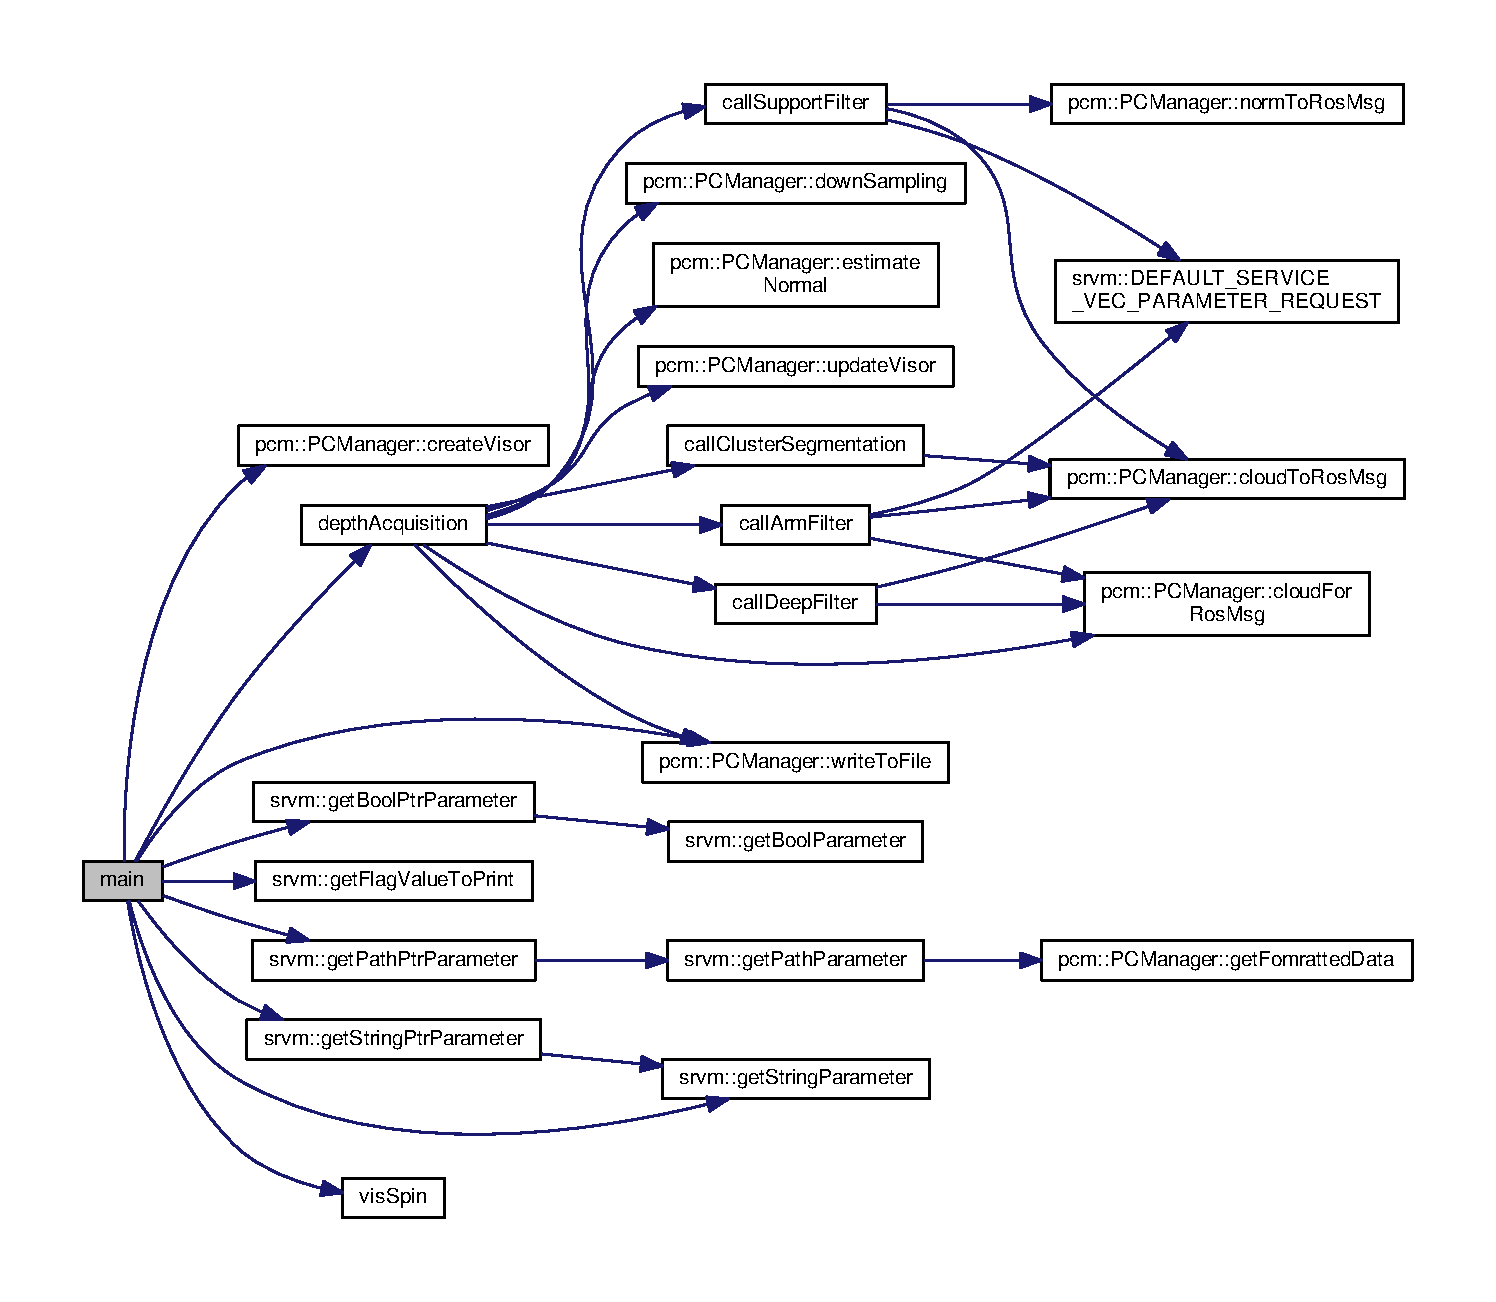
\includegraphics[width=350pt]{obj__segmentation_8cpp_a3c04138a5bfe5d72780bb7e82a18e627_cgraph}
\end{center}
\end{figure}


\hypertarget{obj__segmentation_8cpp_aca73ab26cae45b4b998a3cca9e4f75bc}{\index{obj\-\_\-segmentation.\-cpp@{obj\-\_\-segmentation.\-cpp}!vis\-Spin@{vis\-Spin}}
\index{vis\-Spin@{vis\-Spin}!obj_segmentation.cpp@{obj\-\_\-segmentation.\-cpp}}
\subsubsection[{vis\-Spin}]{\setlength{\rightskip}{0pt plus 5cm}void vis\-Spin (
\begin{DoxyParamCaption}
{}
\end{DoxyParamCaption}
)}}\label{obj__segmentation_8cpp_aca73ab26cae45b4b998a3cca9e4f75bc}


make the visualisation spinning without lagging acroos multi updating. 



Definition at line 192 of file obj\-\_\-segmentation.\-cpp.



References vis, and vis\-\_\-mutex.



Referenced by main().



\subsection{Variable Documentation}
\hypertarget{obj__segmentation_8cpp_a6317446c893a78108aab89bf69a4b66a}{\index{obj\-\_\-segmentation.\-cpp@{obj\-\_\-segmentation.\-cpp}!centroid\-Log\-File\-Path@{centroid\-Log\-File\-Path}}
\index{centroid\-Log\-File\-Path@{centroid\-Log\-File\-Path}!obj_segmentation.cpp@{obj\-\_\-segmentation.\-cpp}}
\subsubsection[{centroid\-Log\-File\-Path}]{\setlength{\rightskip}{0pt plus 5cm}string centroid\-Log\-File\-Path}}\label{obj__segmentation_8cpp_a6317446c893a78108aab89bf69a4b66a}


file path to lag the centroids of the acquired objects in a table. Set to empty to do not log on file. 

The data, that will be appended on the file for each acquisition will have the following shape\-: 
\begin{DoxyCode}
\textcolor{stringliteral}{"scan id, support idx, cluster idx, centroid X, centroid Y, centroid Z;\(\backslash\)n"} 
\end{DoxyCode}


This is a global input parameter that is settable from launcher and acquired during node initialization (see also \hyperlink{obj__segmentation_8cpp_a3c04138a5bfe5d72780bb7e82a18e627}{main} function\-: argv\mbox{[} 6\mbox{]}). \par
 It cannot be changed on the fly. \par
 It default values is set to\-: \hyperlink{namespacesrvm_a92921b8b79655fa69a697a54dca42056}{srvm\-::\-D\-E\-F\-A\-U\-L\-T\-\_\-\-I\-N\-P\-U\-T\-\_\-\-P\-A\-R\-A\-M\-\_\-\-C\-E\-N\-T\-R\-O\-I\-D\-\_\-\-L\-O\-G\-\_\-\-F\-I\-L\-E} 

Definition at line 156 of file obj\-\_\-segmentation.\-cpp.



Referenced by depth\-Acquisition(), and main().

\hypertarget{obj__segmentation_8cpp_a431711d7fd270977af34b226ed5d5cef}{\index{obj\-\_\-segmentation.\-cpp@{obj\-\_\-segmentation.\-cpp}!cluster\-Pub@{cluster\-Pub}}
\index{cluster\-Pub@{cluster\-Pub}!obj_segmentation.cpp@{obj\-\_\-segmentation.\-cpp}}
\subsubsection[{cluster\-Pub}]{\setlength{\rightskip}{0pt plus 5cm}ros\-::\-Publisher cluster\-Pub}}\label{obj__segmentation_8cpp_a431711d7fd270977af34b226ed5d5cef}


the R\-O\-S publisher in which the message of a new acquistion will be send. 

Its name is\-: \hyperlink{namespacesrvm_a520b8813dc65ba764d59f05a0b316e5c}{srvm\-::\-T\-O\-P\-I\-C\-\_\-\-O\-U\-T\-\_\-\-N\-A\-M\-E\-\_\-\-O\-B\-J\-E\-C\-T\-\_\-\-P\-E\-R\-C\-E\-P\-T\-I\-O\-N}. 

Definition at line 171 of file obj\-\_\-segmentation.\-cpp.



Referenced by depth\-Acquisition(), and main().

\hypertarget{obj__segmentation_8cpp_ab64cbde8b32aa3524e9fb94bb4d24525}{\index{obj\-\_\-segmentation.\-cpp@{obj\-\_\-segmentation.\-cpp}!input\-Show\-Cluster\-Clouds@{input\-Show\-Cluster\-Clouds}}
\index{input\-Show\-Cluster\-Clouds@{input\-Show\-Cluster\-Clouds}!obj_segmentation.cpp@{obj\-\_\-segmentation.\-cpp}}
\subsubsection[{input\-Show\-Cluster\-Clouds}]{\setlength{\rightskip}{0pt plus 5cm}bool input\-Show\-Cluster\-Clouds}}\label{obj__segmentation_8cpp_ab64cbde8b32aa3524e9fb94bb4d24525}


flag for showing identified objects (random colors) on the visualiser of this node. 

This is a global input parameter that is settable from launcher and acquired during node initialization (see also \hyperlink{obj__segmentation_8cpp_a3c04138a5bfe5d72780bb7e82a18e627}{main} function\-: argv\mbox{[} 4\mbox{]}). \par
 It cannot be changed on the fly. \par
 It default values is set to\-: \hyperlink{namespacesrvm_aef053199a3f95b1da712ef187b096f93}{srvm\-::\-D\-E\-F\-A\-U\-L\-T\-\_\-\-I\-N\-P\-U\-T\-\_\-\-P\-A\-R\-A\-M\-\_\-\-S\-H\-O\-W\-\_\-\-C\-L\-U\-S\-T\-E\-R\-S} 

Definition at line 135 of file obj\-\_\-segmentation.\-cpp.



Referenced by call\-Deep\-Filter(), call\-Support\-Filter(), depth\-Acquisition(), and main().

\hypertarget{obj__segmentation_8cpp_aea198f61928e89fc5332d092619b04f5}{\index{obj\-\_\-segmentation.\-cpp@{obj\-\_\-segmentation.\-cpp}!input\-Show\-Object\-On\-Support@{input\-Show\-Object\-On\-Support}}
\index{input\-Show\-Object\-On\-Support@{input\-Show\-Object\-On\-Support}!obj_segmentation.cpp@{obj\-\_\-segmentation.\-cpp}}
\subsubsection[{input\-Show\-Object\-On\-Support}]{\setlength{\rightskip}{0pt plus 5cm}bool input\-Show\-Object\-On\-Support}}\label{obj__segmentation_8cpp_aea198f61928e89fc5332d092619b04f5}


flag for showing identified all the points on the table (orange points) on the visualiser of this node. 

This is a global input parameter that is settable from launcher and acquired during node initialization (see also \hyperlink{obj__segmentation_8cpp_a3c04138a5bfe5d72780bb7e82a18e627}{main} function\-: argv\mbox{[} 5\mbox{]}). \par
 It cannot be changed on the fly. \par
 It default values is set to\-: \hyperlink{namespacesrvm_a8e6760e3e9557fc2fb87cbb6fcd8b3e6}{srvm\-::\-D\-E\-F\-A\-U\-L\-T\-\_\-\-I\-N\-P\-U\-T\-\_\-\-P\-A\-R\-A\-M\-\_\-\-S\-H\-O\-W\-\_\-\-O\-B\-J\-E\-C\-T\-\_\-\-O\-N\-\_\-\-S\-U\-P\-P\-O\-R\-T} 

Definition at line 144 of file obj\-\_\-segmentation.\-cpp.



Referenced by call\-Deep\-Filter(), call\-Support\-Filter(), depth\-Acquisition(), and main().

\hypertarget{obj__segmentation_8cpp_ac6f703bc9e7358560334737266db326c}{\index{obj\-\_\-segmentation.\-cpp@{obj\-\_\-segmentation.\-cpp}!input\-Show\-Original\-Cloud@{input\-Show\-Original\-Cloud}}
\index{input\-Show\-Original\-Cloud@{input\-Show\-Original\-Cloud}!obj_segmentation.cpp@{obj\-\_\-segmentation.\-cpp}}
\subsubsection[{input\-Show\-Original\-Cloud}]{\setlength{\rightskip}{0pt plus 5cm}bool input\-Show\-Original\-Cloud}}\label{obj__segmentation_8cpp_ac6f703bc9e7358560334737266db326c}


flag for showing raw cloud (white points) on the visualiser of this node. 

This is a global input parameter that is settable from launcher and acquired during node initialization (see also \hyperlink{obj__segmentation_8cpp_a3c04138a5bfe5d72780bb7e82a18e627}{main} function\-: argv\mbox{[} 2\mbox{]}). \par
 It cannot be changed on the fly. \par
 It default values is set to\-: \hyperlink{namespacesrvm_ac54afc31491c977345ef1a1fbb563be3}{srvm\-::\-D\-E\-F\-A\-U\-L\-T\-\_\-\-I\-N\-P\-U\-T\-\_\-\-P\-A\-R\-A\-M\-\_\-\-S\-H\-O\-W\-\_\-\-O\-R\-I\-G\-I\-N\-A\-L\-\_\-\-C\-L\-O\-U\-D} 

Definition at line 117 of file obj\-\_\-segmentation.\-cpp.



Referenced by call\-Deep\-Filter(), call\-Support\-Filter(), depth\-Acquisition(), and main().

\hypertarget{obj__segmentation_8cpp_acece8259b4a7b4327562daa817a43ef0}{\index{obj\-\_\-segmentation.\-cpp@{obj\-\_\-segmentation.\-cpp}!input\-Show\-Support\-Clouds@{input\-Show\-Support\-Clouds}}
\index{input\-Show\-Support\-Clouds@{input\-Show\-Support\-Clouds}!obj_segmentation.cpp@{obj\-\_\-segmentation.\-cpp}}
\subsubsection[{input\-Show\-Support\-Clouds}]{\setlength{\rightskip}{0pt plus 5cm}bool input\-Show\-Support\-Clouds}}\label{obj__segmentation_8cpp_acece8259b4a7b4327562daa817a43ef0}


flag for showing identified tables (brown points) on the visualiser of this node. 

This is a global input parameter that is settable from launcher and acquired during node initialization (see also \hyperlink{obj__segmentation_8cpp_a3c04138a5bfe5d72780bb7e82a18e627}{main} function\-: argv\mbox{[} 3\mbox{]}). \par
 It cannot be changed on the fly. \par
 It default values is set to\-: \hyperlink{namespacesrvm_a9880144ef0df953c3b583e4f20dbff76}{srvm\-::\-D\-E\-F\-A\-U\-L\-T\-\_\-\-I\-N\-P\-U\-T\-\_\-\-P\-A\-R\-A\-M\-\_\-\-S\-H\-O\-W\-\_\-\-S\-U\-P\-P\-O\-R\-T\-S} 

Definition at line 126 of file obj\-\_\-segmentation.\-cpp.



Referenced by call\-Deep\-Filter(), call\-Support\-Filter(), depth\-Acquisition(), and main().

\hypertarget{obj__segmentation_8cpp_a484374fe771cd860a2ea9f9feda68905}{\index{obj\-\_\-segmentation.\-cpp@{obj\-\_\-segmentation.\-cpp}!log\-\_\-str\-\_\-depth@{log\-\_\-str\-\_\-depth}}
\index{log\-\_\-str\-\_\-depth@{log\-\_\-str\-\_\-depth}!obj_segmentation.cpp@{obj\-\_\-segmentation.\-cpp}}
\subsubsection[{log\-\_\-str\-\_\-depth}]{\setlength{\rightskip}{0pt plus 5cm}string log\-\_\-str\-\_\-depth = \char`\"{}Loading...\char`\"{}}}\label{obj__segmentation_8cpp_a484374fe771cd860a2ea9f9feda68905}


string that will contains info about \hyperlink{deep__filter__srv_8cpp}{deep\-\_\-filter\-\_\-srv.\-cpp} service, shown in the visualiser while the parameters are changed on the fly. 



Definition at line 179 of file obj\-\_\-segmentation.\-cpp.



Referenced by call\-Deep\-Filter(), and main().

\hypertarget{obj__segmentation_8cpp_a7024ef4623a4562d025033aa950364f5}{\index{obj\-\_\-segmentation.\-cpp@{obj\-\_\-segmentation.\-cpp}!log\-\_\-str\-\_\-supp@{log\-\_\-str\-\_\-supp}}
\index{log\-\_\-str\-\_\-supp@{log\-\_\-str\-\_\-supp}!obj_segmentation.cpp@{obj\-\_\-segmentation.\-cpp}}
\subsubsection[{log\-\_\-str\-\_\-supp}]{\setlength{\rightskip}{0pt plus 5cm}string log\-\_\-str\-\_\-supp = \char`\"{}Loading...\char`\"{}}}\label{obj__segmentation_8cpp_a7024ef4623a4562d025033aa950364f5}


string that will contains info about support\-\_\-segmentation\-\_\-srv.\-cpp service, shown in the visualiser while the parameters are changed on the fly. 



Definition at line 181 of file obj\-\_\-segmentation.\-cpp.



Referenced by call\-Support\-Filter(), and main().

\hypertarget{obj__segmentation_8cpp_a21221f555fa05f2c3f45ff5592a25197}{\index{obj\-\_\-segmentation.\-cpp@{obj\-\_\-segmentation.\-cpp}!manager@{manager}}
\index{manager@{manager}!obj_segmentation.cpp@{obj\-\_\-segmentation.\-cpp}}
\subsubsection[{manager}]{\setlength{\rightskip}{0pt plus 5cm}{\bf pcm\-::\-P\-C\-Manager}$\ast$ manager = new {\bf pcm\-::\-P\-C\-Manager}( false)}}\label{obj__segmentation_8cpp_a21221f555fa05f2c3f45ff5592a25197}


variable to initialise the \hyperlink{classpcm_1_1PCManager}{pcm\-::\-P\-C\-Manager}. 



Definition at line 165 of file obj\-\_\-segmentation.\-cpp.

\hypertarget{obj__segmentation_8cpp_a3fea3689c92e1b2fcebd3eeafee94a5e}{\index{obj\-\_\-segmentation.\-cpp@{obj\-\_\-segmentation.\-cpp}!M\-I\-N\-\_\-\-P\-O\-I\-N\-T\-\_\-\-I\-N\-\_\-\-O\-R\-I\-G\-I\-N\-A\-L\-\_\-\-C\-L\-O\-U\-D@{M\-I\-N\-\_\-\-P\-O\-I\-N\-T\-\_\-\-I\-N\-\_\-\-O\-R\-I\-G\-I\-N\-A\-L\-\_\-\-C\-L\-O\-U\-D}}
\index{M\-I\-N\-\_\-\-P\-O\-I\-N\-T\-\_\-\-I\-N\-\_\-\-O\-R\-I\-G\-I\-N\-A\-L\-\_\-\-C\-L\-O\-U\-D@{M\-I\-N\-\_\-\-P\-O\-I\-N\-T\-\_\-\-I\-N\-\_\-\-O\-R\-I\-G\-I\-N\-A\-L\-\_\-\-C\-L\-O\-U\-D}!obj_segmentation.cpp@{obj\-\_\-segmentation.\-cpp}}
\subsubsection[{M\-I\-N\-\_\-\-P\-O\-I\-N\-T\-\_\-\-I\-N\-\_\-\-O\-R\-I\-G\-I\-N\-A\-L\-\_\-\-C\-L\-O\-U\-D}]{\setlength{\rightskip}{0pt plus 5cm}const int M\-I\-N\-\_\-\-P\-O\-I\-N\-T\-\_\-\-I\-N\-\_\-\-O\-R\-I\-G\-I\-N\-A\-L\-\_\-\-C\-L\-O\-U\-D = 30\hspace{0.3cm}{\ttfamily [static]}}}\label{obj__segmentation_8cpp_a3fea3689c92e1b2fcebd3eeafee94a5e}


the cloud will be not not processed if has less number of points 



Definition at line 101 of file obj\-\_\-segmentation.\-cpp.



Referenced by depth\-Acquisition().

\hypertarget{obj__segmentation_8cpp_afe3fec681d3658d114dfa8cfff163e82}{\index{obj\-\_\-segmentation.\-cpp@{obj\-\_\-segmentation.\-cpp}!nh\-\_\-ptr@{nh\-\_\-ptr}}
\index{nh\-\_\-ptr@{nh\-\_\-ptr}!obj_segmentation.cpp@{obj\-\_\-segmentation.\-cpp}}
\subsubsection[{nh\-\_\-ptr}]{\setlength{\rightskip}{0pt plus 5cm}ros\-::\-Node\-Handle$\ast$ nh\-\_\-ptr = N\-U\-L\-L}}\label{obj__segmentation_8cpp_afe3fec681d3658d114dfa8cfff163e82}


ros handle passed across all services calls. 



Definition at line 167 of file obj\-\_\-segmentation.\-cpp.



Referenced by call\-Arm\-Filter(), call\-Cluster\-Segmentation(), call\-Deep\-Filter(), call\-Support\-Filter(), and main().

\hypertarget{obj__segmentation_8cpp_abeb91134d7b10cc7475f7fa946e66a34}{\index{obj\-\_\-segmentation.\-cpp@{obj\-\_\-segmentation.\-cpp}!pcl\-Transform@{pcl\-Transform}}
\index{pcl\-Transform@{pcl\-Transform}!obj_segmentation.cpp@{obj\-\_\-segmentation.\-cpp}}
\subsubsection[{pcl\-Transform}]{\setlength{\rightskip}{0pt plus 5cm}Eigen\-::\-Matrix4f pcl\-Transform}}\label{obj__segmentation_8cpp_abeb91134d7b10cc7475f7fa946e66a34}


the transformation matrix between the R\-G\-B-\/\-D sensor and the \hyperlink{namespacesrvm_ac5228e86d6d396c944b11f847746b3b8}{srvm\-::\-P\-A\-R\-A\-M\-\_\-\-N\-A\-M\-E\-\_\-\-I\-N\-P\-U\-T\-\_\-\-C\-L\-O\-U\-D\-\_\-\-R\-E\-F\-E\-R\-E\-N\-C\-E\-\_\-\-F\-R\-A\-M\-E} frame (it can be changed on the fly). 



Definition at line 173 of file obj\-\_\-segmentation.\-cpp.



Referenced by depth\-Acquisition(), and main().

\hypertarget{obj__segmentation_8cpp_a848f9977cb150e83cf5464a65dcc9fe4}{\index{obj\-\_\-segmentation.\-cpp@{obj\-\_\-segmentation.\-cpp}!scan\-Id@{scan\-Id}}
\index{scan\-Id@{scan\-Id}!obj_segmentation.cpp@{obj\-\_\-segmentation.\-cpp}}
\subsubsection[{scan\-Id}]{\setlength{\rightskip}{0pt plus 5cm}long scan\-Id = 0}}\label{obj__segmentation_8cpp_a848f9977cb150e83cf5464a65dcc9fe4}


so far, it is used only for logging. 



Definition at line 183 of file obj\-\_\-segmentation.\-cpp.



Referenced by depth\-Acquisition().

\hypertarget{obj__segmentation_8cpp_a6c2d87234fca8dcca11f888098558986}{\index{obj\-\_\-segmentation.\-cpp@{obj\-\_\-segmentation.\-cpp}!vis@{vis}}
\index{vis@{vis}!obj_segmentation.cpp@{obj\-\_\-segmentation.\-cpp}}
\subsubsection[{vis}]{\setlength{\rightskip}{0pt plus 5cm}boost\-::shared\-\_\-ptr$<$ {\bf visualization\-::\-P\-C\-L\-Visualizer}$>$ vis}}\label{obj__segmentation_8cpp_a6c2d87234fca8dcca11f888098558986}


the P\-C\-L visualiser for this node. 

It will happear if at least one of\-: \hyperlink{obj__segmentation_8cpp_ac6f703bc9e7358560334737266db326c}{input\-Show\-Original\-Cloud}, \hyperlink{obj__segmentation_8cpp_acece8259b4a7b4327562daa817a43ef0}{input\-Show\-Support\-Clouds}, \hyperlink{obj__segmentation_8cpp_ab64cbde8b32aa3524e9fb94bb4d24525}{input\-Show\-Cluster\-Clouds}, \hyperlink{obj__segmentation_8cpp_aea198f61928e89fc5332d092619b04f5}{input\-Show\-Object\-On\-Support}; is true. 

Definition at line 169 of file obj\-\_\-segmentation.\-cpp.



Referenced by call\-Deep\-Filter(), call\-Support\-Filter(), depth\-Acquisition(), main(), and vis\-Spin().

\hypertarget{obj__segmentation_8cpp_a0dc8882293908d9c8cc15f76a2a49588}{\index{obj\-\_\-segmentation.\-cpp@{obj\-\_\-segmentation.\-cpp}!vis\-\_\-mutex@{vis\-\_\-mutex}}
\index{vis\-\_\-mutex@{vis\-\_\-mutex}!obj_segmentation.cpp@{obj\-\_\-segmentation.\-cpp}}
\subsubsection[{vis\-\_\-mutex}]{\setlength{\rightskip}{0pt plus 5cm}boost\-::mutex vis\-\_\-mutex}}\label{obj__segmentation_8cpp_a0dc8882293908d9c8cc15f76a2a49588}


for a better visualiser updating during different services calls. 



Definition at line 177 of file obj\-\_\-segmentation.\-cpp.



Referenced by call\-Deep\-Filter(), call\-Support\-Filter(), depth\-Acquisition(), and vis\-Spin().

\hypertarget{obj__segmentation_8cpp_ab83e6219895a4d26706c0d858f8ec288}{\index{obj\-\_\-segmentation.\-cpp@{obj\-\_\-segmentation.\-cpp}!vis\-\_\-thread@{vis\-\_\-thread}}
\index{vis\-\_\-thread@{vis\-\_\-thread}!obj_segmentation.cpp@{obj\-\_\-segmentation.\-cpp}}
\subsubsection[{vis\-\_\-thread}]{\setlength{\rightskip}{0pt plus 5cm}boost\-::thread vis\-\_\-thread}}\label{obj__segmentation_8cpp_ab83e6219895a4d26706c0d858f8ec288}


for a better visualiser updating on parallel thread. 



Definition at line 175 of file obj\-\_\-segmentation.\-cpp.



Referenced by main().


\hypertarget{pc__manager_8cpp}{\section{src/point\-\_\-cloud\-\_\-library/pc\-\_\-manager.cpp File Reference}
\label{pc__manager_8cpp}\index{src/point\-\_\-cloud\-\_\-library/pc\-\_\-manager.\-cpp@{src/point\-\_\-cloud\-\_\-library/pc\-\_\-manager.\-cpp}}
}
{\ttfamily \#include \char`\"{}../point\-\_\-cloud\-\_\-library/pc\-\_\-manager.\-h\char`\"{}}\\*
Include dependency graph for pc\-\_\-manager.\-cpp\-:\nopagebreak
\begin{figure}[H]
\begin{center}
\leavevmode
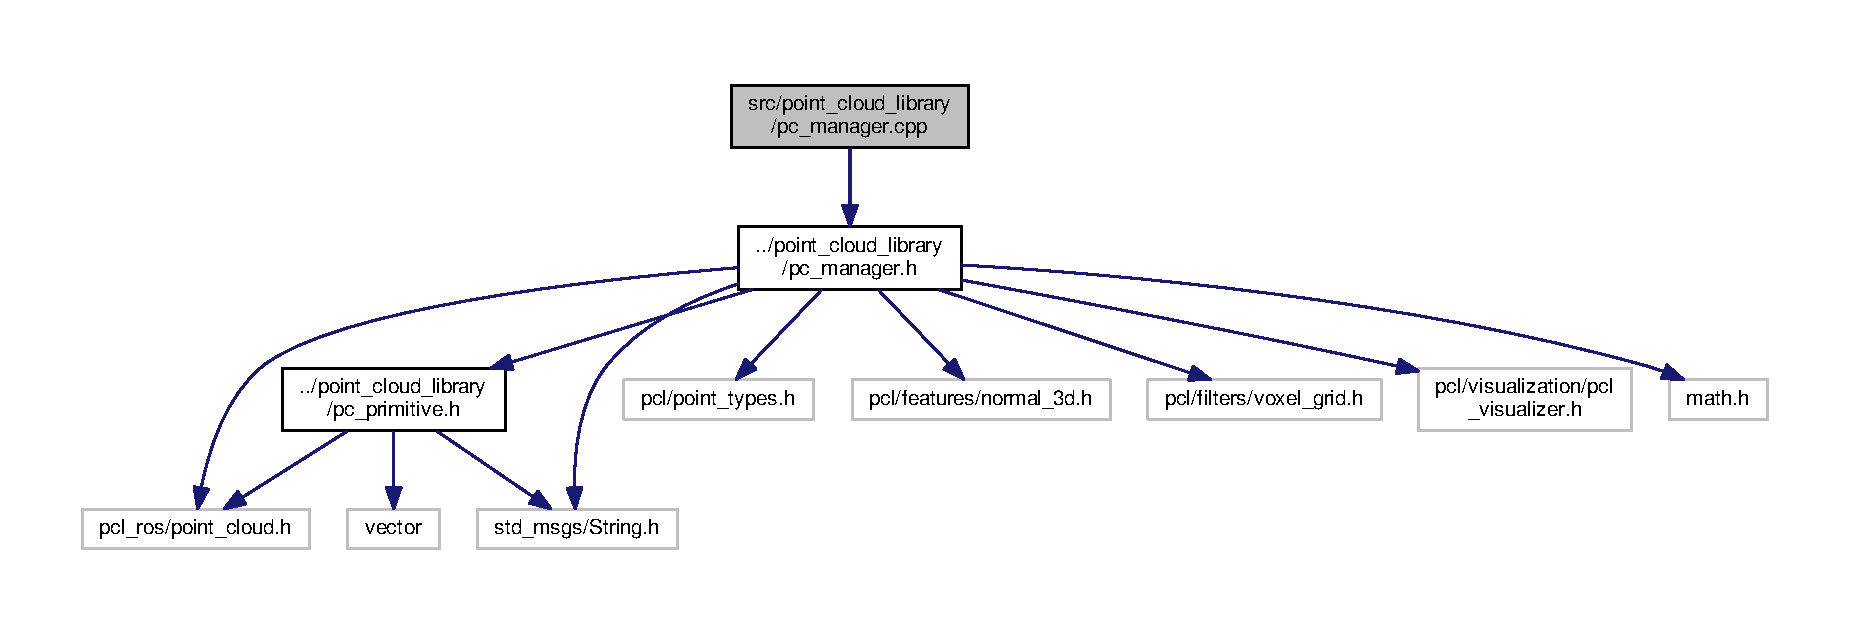
\includegraphics[width=350pt]{pc__manager_8cpp__incl}
\end{center}
\end{figure}
\subsection*{Namespaces}
\begin{DoxyCompactItemize}
\item 
\hyperlink{namespacepcm}{pcm}
\end{DoxyCompactItemize}
\subsection*{Functions}
\begin{DoxyCompactItemize}
\item 
static search\-::\-Kd\-Tree\\*
$<$ Point\-X\-Y\-Z $>$\-::Ptr \hyperlink{namespacepcm_a6db83da07339681645ba19a92dbd2046}{pcm\-::tree} (new search\-::\-Kd\-Tree$<$ Point\-X\-Y\-Z $>$())
\end{DoxyCompactItemize}
\subsection*{Variables}
\begin{DoxyCompactItemize}
\item 
static Normal\-Estimation\\*
$<$ Point\-X\-Y\-Z, Normal $>$ \hyperlink{namespacepcm_acbfa006c5c9699694cdf4f598ff57165}{pcm\-::ne}
\item 
static Voxel\-Grid$<$ Point\-X\-Y\-Z $>$ \hyperlink{namespacepcm_a55d9cba2f3ff7122f9162542cde192ac}{pcm\-::sor}
\end{DoxyCompactItemize}

\hypertarget{pc__manager_8h}{\section{src/point\-\_\-cloud\-\_\-library/pc\-\_\-manager.h File Reference}
\label{pc__manager_8h}\index{src/point\-\_\-cloud\-\_\-library/pc\-\_\-manager.\-h@{src/point\-\_\-cloud\-\_\-library/pc\-\_\-manager.\-h}}
}
{\ttfamily \#include $<$pcl\-\_\-ros/point\-\_\-cloud.\-h$>$}\\*
{\ttfamily \#include $<$pcl/point\-\_\-types.\-h$>$}\\*
{\ttfamily \#include $<$pcl/features/normal\-\_\-3d.\-h$>$}\\*
{\ttfamily \#include $<$pcl/filters/voxel\-\_\-grid.\-h$>$}\\*
{\ttfamily \#include $<$pcl/visualization/pcl\-\_\-visualizer.\-h$>$}\\*
{\ttfamily \#include $<$std\-\_\-msgs/\-String.\-h$>$}\\*
{\ttfamily \#include $<$math.\-h$>$}\\*
{\ttfamily \#include \char`\"{}../point\-\_\-cloud\-\_\-library/pc\-\_\-primitive.\-h\char`\"{}}\\*
Include dependency graph for pc\-\_\-manager.\-h\-:\nopagebreak
\begin{figure}[H]
\begin{center}
\leavevmode
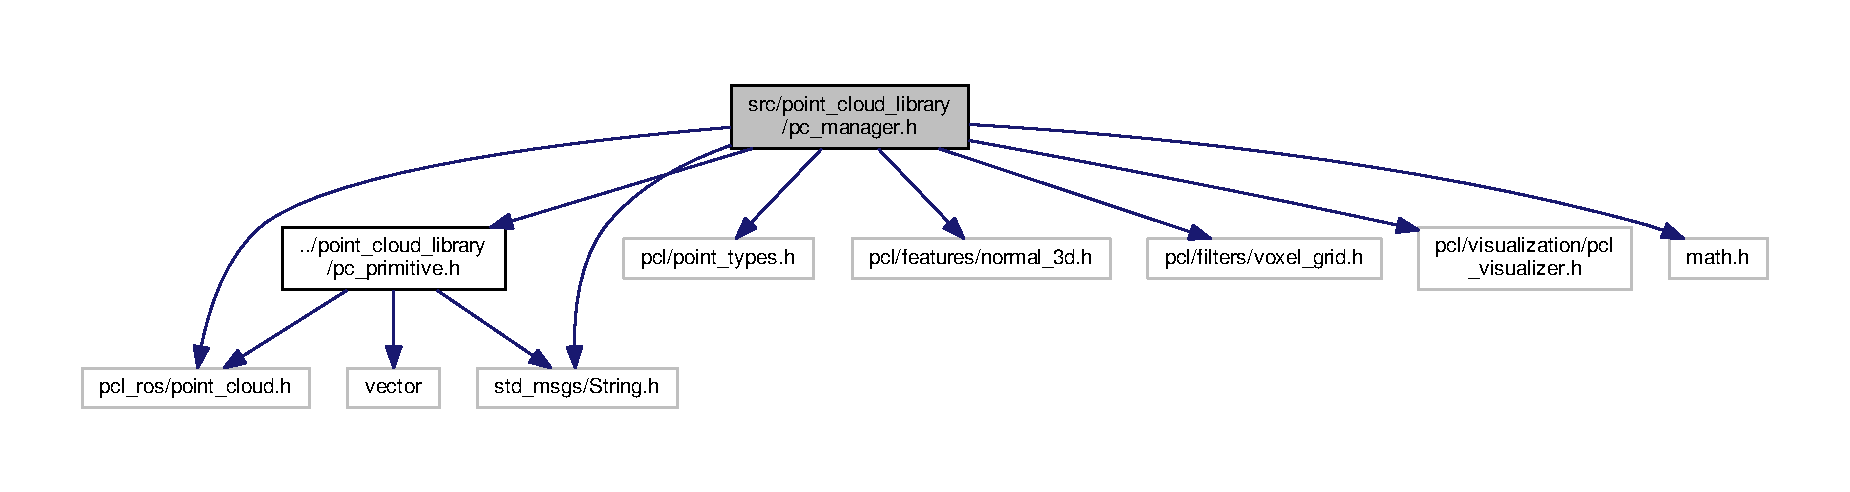
\includegraphics[width=350pt]{pc__manager_8h__incl}
\end{center}
\end{figure}
This graph shows which files directly or indirectly include this file\-:\nopagebreak
\begin{figure}[H]
\begin{center}
\leavevmode
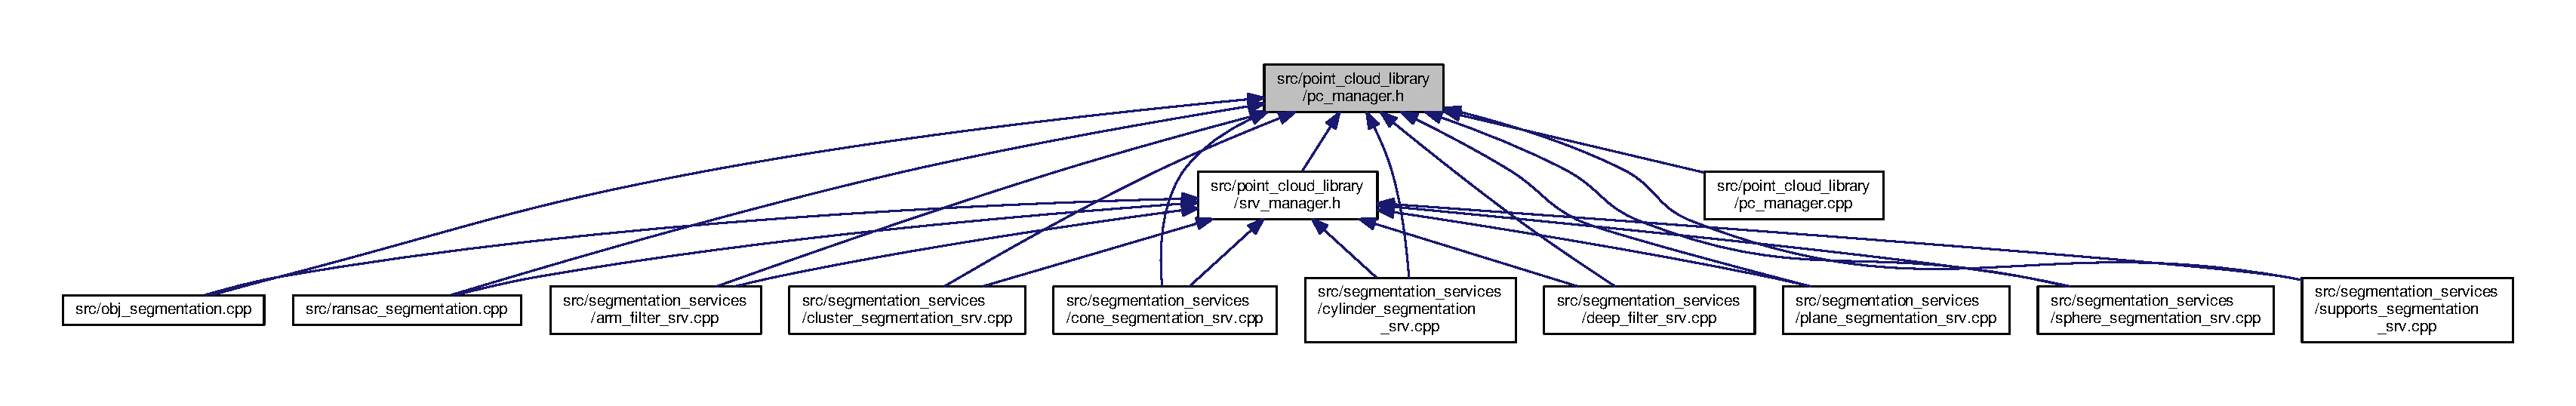
\includegraphics[width=350pt]{pc__manager_8h__dep__incl}
\end{center}
\end{figure}
\subsection*{Classes}
\begin{DoxyCompactItemize}
\item 
class \hyperlink{classpcm_1_1PCManager}{pcm\-::\-P\-C\-Manager}
\end{DoxyCompactItemize}
\subsection*{Namespaces}
\begin{DoxyCompactItemize}
\item 
\hyperlink{namespacepcm}{pcm}
\end{DoxyCompactItemize}
\subsection*{Typedefs}
\begin{DoxyCompactItemize}
\item 
typedef boost\-::shared\-\_\-ptr\\*
$<$ \hyperlink{classpcp_1_1PCPrimitive}{pcp\-::\-P\-C\-Primitive} $>$ \hyperlink{pc__manager_8h_a0976ac6881bc2fcf1a5503663203e83f}{P\-C\-Primitive\-Ptr}
\item 
typedef boost\-::shared\-\_\-ptr\\*
$<$ visualization\-::\-P\-C\-L\-Visualizer $>$ \hyperlink{pc__manager_8h_a38c805dbc7ad6f06109b85c8e540817a}{P\-C\-L\-Visualizer}
\end{DoxyCompactItemize}


\subsection{Typedef Documentation}
\hypertarget{pc__manager_8h_a38c805dbc7ad6f06109b85c8e540817a}{\index{pc\-\_\-manager.\-h@{pc\-\_\-manager.\-h}!P\-C\-L\-Visualizer@{P\-C\-L\-Visualizer}}
\index{P\-C\-L\-Visualizer@{P\-C\-L\-Visualizer}!pc_manager.h@{pc\-\_\-manager.\-h}}
\subsubsection[{P\-C\-L\-Visualizer}]{\setlength{\rightskip}{0pt plus 5cm}typedef boost\-::shared\-\_\-ptr$<$ visualization\-::\-P\-C\-L\-Visualizer$>$ {\bf P\-C\-L\-Visualizer}}}\label{pc__manager_8h_a38c805dbc7ad6f06109b85c8e540817a}


Definition at line 23 of file pc\-\_\-manager.\-h.

\hypertarget{pc__manager_8h_a0976ac6881bc2fcf1a5503663203e83f}{\index{pc\-\_\-manager.\-h@{pc\-\_\-manager.\-h}!P\-C\-Primitive\-Ptr@{P\-C\-Primitive\-Ptr}}
\index{P\-C\-Primitive\-Ptr@{P\-C\-Primitive\-Ptr}!pc_manager.h@{pc\-\_\-manager.\-h}}
\subsubsection[{P\-C\-Primitive\-Ptr}]{\setlength{\rightskip}{0pt plus 5cm}typedef boost\-::shared\-\_\-ptr$<$ {\bf pcp\-::\-P\-C\-Primitive}$>$ {\bf P\-C\-Primitive\-Ptr}}}\label{pc__manager_8h_a0976ac6881bc2fcf1a5503663203e83f}


Definition at line 22 of file pc\-\_\-manager.\-h.


\hypertarget{pc__primitive_8cpp}{\section{src/point\-\_\-cloud\-\_\-library/pc\-\_\-primitive.cpp File Reference}
\label{pc__primitive_8cpp}\index{src/point\-\_\-cloud\-\_\-library/pc\-\_\-primitive.\-cpp@{src/point\-\_\-cloud\-\_\-library/pc\-\_\-primitive.\-cpp}}
}
{\ttfamily \#include \char`\"{}../point\-\_\-cloud\-\_\-library/pc\-\_\-primitive.\-h\char`\"{}}\\*
Include dependency graph for pc\-\_\-primitive.\-cpp\-:\nopagebreak
\begin{figure}[H]
\begin{center}
\leavevmode
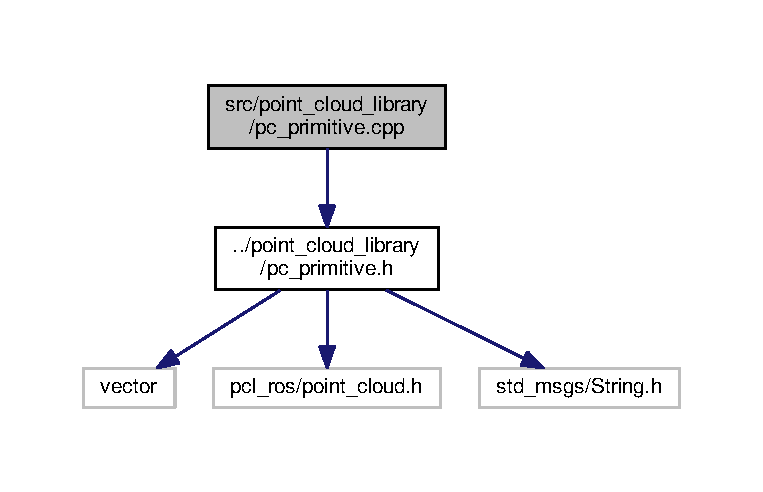
\includegraphics[width=350pt]{pc__primitive_8cpp__incl}
\end{center}
\end{figure}
\subsection*{Namespaces}
\begin{DoxyCompactItemize}
\item 
\hyperlink{namespacepcp}{pcp}
\end{DoxyCompactItemize}

\hypertarget{pc__primitive_8h}{\section{src/point\-\_\-cloud\-\_\-library/pc\-\_\-primitive.h File Reference}
\label{pc__primitive_8h}\index{src/point\-\_\-cloud\-\_\-library/pc\-\_\-primitive.\-h@{src/point\-\_\-cloud\-\_\-library/pc\-\_\-primitive.\-h}}
}
{\ttfamily \#include $<$vector$>$}\\*
{\ttfamily \#include $<$pcl\-\_\-ros/point\-\_\-cloud.\-h$>$}\\*
{\ttfamily \#include $<$std\-\_\-msgs/\-String.\-h$>$}\\*
Include dependency graph for pc\-\_\-primitive.\-h\-:
\nopagebreak
\begin{figure}[H]
\begin{center}
\leavevmode
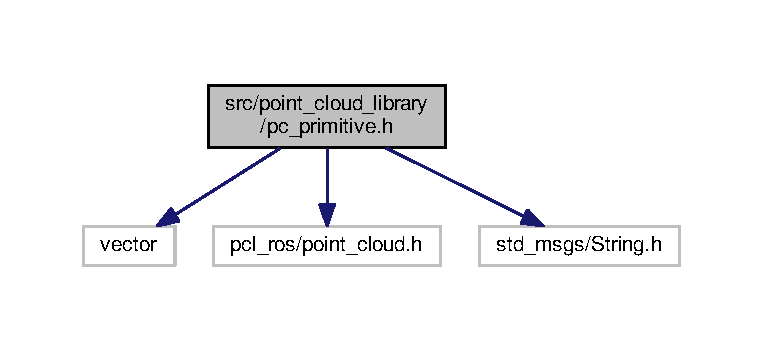
\includegraphics[width=350pt]{pc__primitive_8h__incl}
\end{center}
\end{figure}
This graph shows which files directly or indirectly include this file\-:
\nopagebreak
\begin{figure}[H]
\begin{center}
\leavevmode
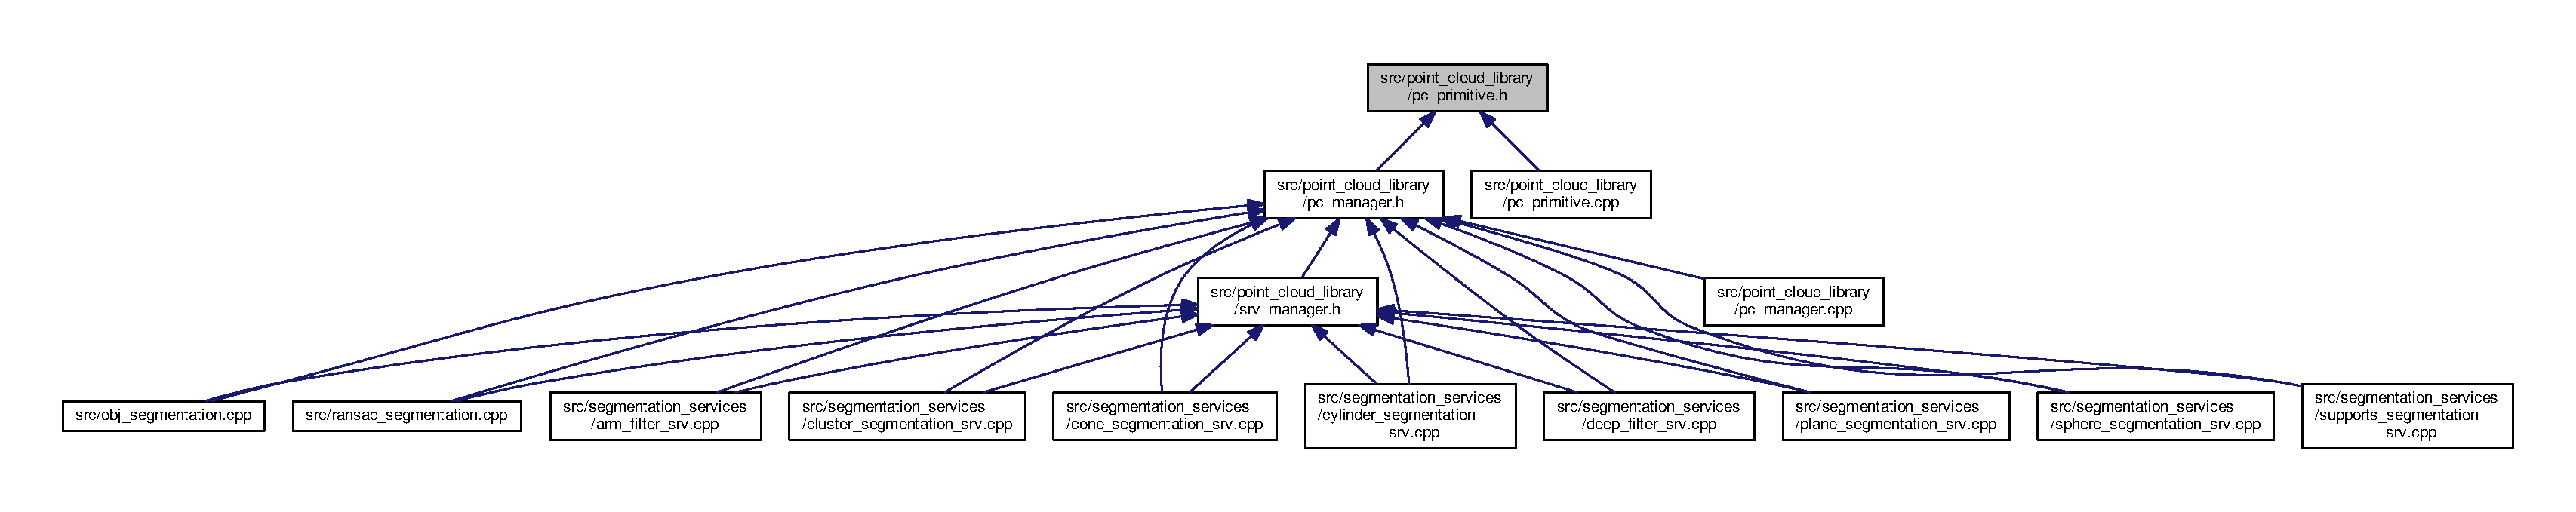
\includegraphics[width=350pt]{pc__primitive_8h__dep__incl}
\end{center}
\end{figure}
\subsection*{Classes}
\begin{DoxyCompactItemize}
\item 
class \hyperlink{classpcp_1_1PCPrimitive}{pcp\-::\-P\-C\-Primitive}
\end{DoxyCompactItemize}
\subsection*{Namespaces}
\begin{DoxyCompactItemize}
\item 
\hyperlink{namespacepcp}{pcp}
\end{DoxyCompactItemize}
\subsection*{Typedefs}
\begin{DoxyCompactItemize}
\item 
typedef std\-::vector$<$ int $>$ \hyperlink{pc__primitive_8h_a9aba110b238bb80390c2545da40823e3}{Primitive\-Idx}
\item 
typedef boost\-::shared\-\_\-ptr\\*
$<$ std\-::vector$<$ int $>$ $>$ \hyperlink{pc__primitive_8h_a6ec0f6fbb026ae4b66cac121673c3a8a}{Primitive\-Idx\-Ptr}
\item 
typedef pcl\-::\-Point\-Cloud\\*
$<$ pcl\-::\-Point\-X\-Y\-Z $>$ \hyperlink{pc__primitive_8h_a02a7c0cdfcd324f1b5b87ce549fdbe10}{P\-C\-L\-Cloud}
\item 
typedef pcl\-::\-Point\-Cloud\\*
$<$ pcl\-::\-Point\-X\-Y\-Z $>$\-::Ptr \hyperlink{pc__primitive_8h_aa14a240c8d999c4f56133c0f70e88783}{P\-C\-L\-Cloud\-Ptr}
\item 
typedef pcl\-::\-Point\-Cloud\\*
$<$ pcl\-::\-Normal $>$ \hyperlink{pc__primitive_8h_abe81b5e6ffcc0ceb1b95b0489419027d}{P\-C\-L\-Normal}
\item 
typedef pcl\-::\-Point\-Cloud\\*
$<$ pcl\-::\-Normal $>$\-::Ptr \hyperlink{pc__primitive_8h_a1bc38ce8b0c26e5f2d28fae9f3e3ea97}{P\-C\-L\-Normal\-Ptr}
\end{DoxyCompactItemize}


\subsection{Typedef Documentation}
\hypertarget{pc__primitive_8h_a02a7c0cdfcd324f1b5b87ce549fdbe10}{\index{pc\-\_\-primitive.\-h@{pc\-\_\-primitive.\-h}!P\-C\-L\-Cloud@{P\-C\-L\-Cloud}}
\index{P\-C\-L\-Cloud@{P\-C\-L\-Cloud}!pc_primitive.h@{pc\-\_\-primitive.\-h}}
\subsubsection[{P\-C\-L\-Cloud}]{\setlength{\rightskip}{0pt plus 5cm}typedef pcl\-::\-Point\-Cloud$<$ pcl\-::\-Point\-X\-Y\-Z$>$ {\bf P\-C\-L\-Cloud}}}\label{pc__primitive_8h_a02a7c0cdfcd324f1b5b87ce549fdbe10}


Definition at line 20 of file pc\-\_\-primitive.\-h.

\hypertarget{pc__primitive_8h_aa14a240c8d999c4f56133c0f70e88783}{\index{pc\-\_\-primitive.\-h@{pc\-\_\-primitive.\-h}!P\-C\-L\-Cloud\-Ptr@{P\-C\-L\-Cloud\-Ptr}}
\index{P\-C\-L\-Cloud\-Ptr@{P\-C\-L\-Cloud\-Ptr}!pc_primitive.h@{pc\-\_\-primitive.\-h}}
\subsubsection[{P\-C\-L\-Cloud\-Ptr}]{\setlength{\rightskip}{0pt plus 5cm}typedef pcl\-::\-Point\-Cloud$<$ pcl\-::\-Point\-X\-Y\-Z$>$\-::Ptr {\bf P\-C\-L\-Cloud\-Ptr}}}\label{pc__primitive_8h_aa14a240c8d999c4f56133c0f70e88783}


Definition at line 21 of file pc\-\_\-primitive.\-h.

\hypertarget{pc__primitive_8h_abe81b5e6ffcc0ceb1b95b0489419027d}{\index{pc\-\_\-primitive.\-h@{pc\-\_\-primitive.\-h}!P\-C\-L\-Normal@{P\-C\-L\-Normal}}
\index{P\-C\-L\-Normal@{P\-C\-L\-Normal}!pc_primitive.h@{pc\-\_\-primitive.\-h}}
\subsubsection[{P\-C\-L\-Normal}]{\setlength{\rightskip}{0pt plus 5cm}typedef pcl\-::\-Point\-Cloud$<$ pcl\-::\-Normal$>$ {\bf P\-C\-L\-Normal}}}\label{pc__primitive_8h_abe81b5e6ffcc0ceb1b95b0489419027d}


Definition at line 22 of file pc\-\_\-primitive.\-h.

\hypertarget{pc__primitive_8h_a1bc38ce8b0c26e5f2d28fae9f3e3ea97}{\index{pc\-\_\-primitive.\-h@{pc\-\_\-primitive.\-h}!P\-C\-L\-Normal\-Ptr@{P\-C\-L\-Normal\-Ptr}}
\index{P\-C\-L\-Normal\-Ptr@{P\-C\-L\-Normal\-Ptr}!pc_primitive.h@{pc\-\_\-primitive.\-h}}
\subsubsection[{P\-C\-L\-Normal\-Ptr}]{\setlength{\rightskip}{0pt plus 5cm}typedef pcl\-::\-Point\-Cloud$<$ pcl\-::\-Normal$>$\-::Ptr {\bf P\-C\-L\-Normal\-Ptr}}}\label{pc__primitive_8h_a1bc38ce8b0c26e5f2d28fae9f3e3ea97}


Definition at line 23 of file pc\-\_\-primitive.\-h.

\hypertarget{pc__primitive_8h_a9aba110b238bb80390c2545da40823e3}{\index{pc\-\_\-primitive.\-h@{pc\-\_\-primitive.\-h}!Primitive\-Idx@{Primitive\-Idx}}
\index{Primitive\-Idx@{Primitive\-Idx}!pc_primitive.h@{pc\-\_\-primitive.\-h}}
\subsubsection[{Primitive\-Idx}]{\setlength{\rightskip}{0pt plus 5cm}typedef std\-::vector$<$ int$>$ {\bf Primitive\-Idx}}}\label{pc__primitive_8h_a9aba110b238bb80390c2545da40823e3}


Definition at line 18 of file pc\-\_\-primitive.\-h.

\hypertarget{pc__primitive_8h_a6ec0f6fbb026ae4b66cac121673c3a8a}{\index{pc\-\_\-primitive.\-h@{pc\-\_\-primitive.\-h}!Primitive\-Idx\-Ptr@{Primitive\-Idx\-Ptr}}
\index{Primitive\-Idx\-Ptr@{Primitive\-Idx\-Ptr}!pc_primitive.h@{pc\-\_\-primitive.\-h}}
\subsubsection[{Primitive\-Idx\-Ptr}]{\setlength{\rightskip}{0pt plus 5cm}typedef boost\-::shared\-\_\-ptr$<$ std\-::vector$<$ int$>$ $>$ {\bf Primitive\-Idx\-Ptr}}}\label{pc__primitive_8h_a6ec0f6fbb026ae4b66cac121673c3a8a}


Definition at line 19 of file pc\-\_\-primitive.\-h.


\hypertarget{srv__manager_8h}{\section{src/point\-\_\-cloud\-\_\-library/srv\-\_\-manager.h File Reference}
\label{srv__manager_8h}\index{src/point\-\_\-cloud\-\_\-library/srv\-\_\-manager.\-h@{src/point\-\_\-cloud\-\_\-library/srv\-\_\-manager.\-h}}
}
{\ttfamily \#include $<$std\-\_\-msgs/\-String.\-h$>$}\\*
{\ttfamily \#include \char`\"{}../point\-\_\-cloud\-\_\-library/pc\-\_\-manager.\-h\char`\"{}}\\*
Include dependency graph for srv\-\_\-manager.\-h\-:
\nopagebreak
\begin{figure}[H]
\begin{center}
\leavevmode
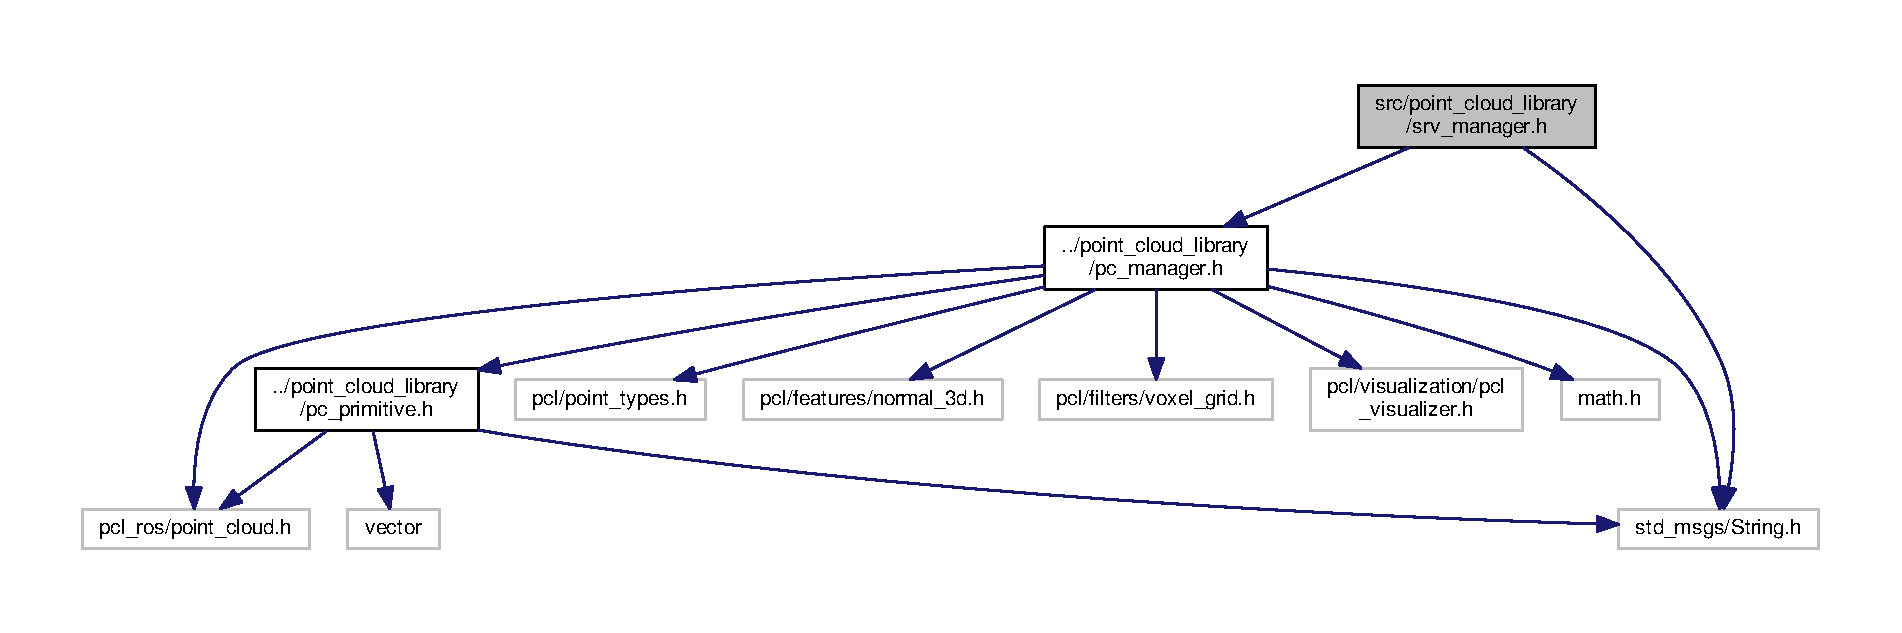
\includegraphics[width=350pt]{srv__manager_8h__incl}
\end{center}
\end{figure}
This graph shows which files directly or indirectly include this file\-:
\nopagebreak
\begin{figure}[H]
\begin{center}
\leavevmode
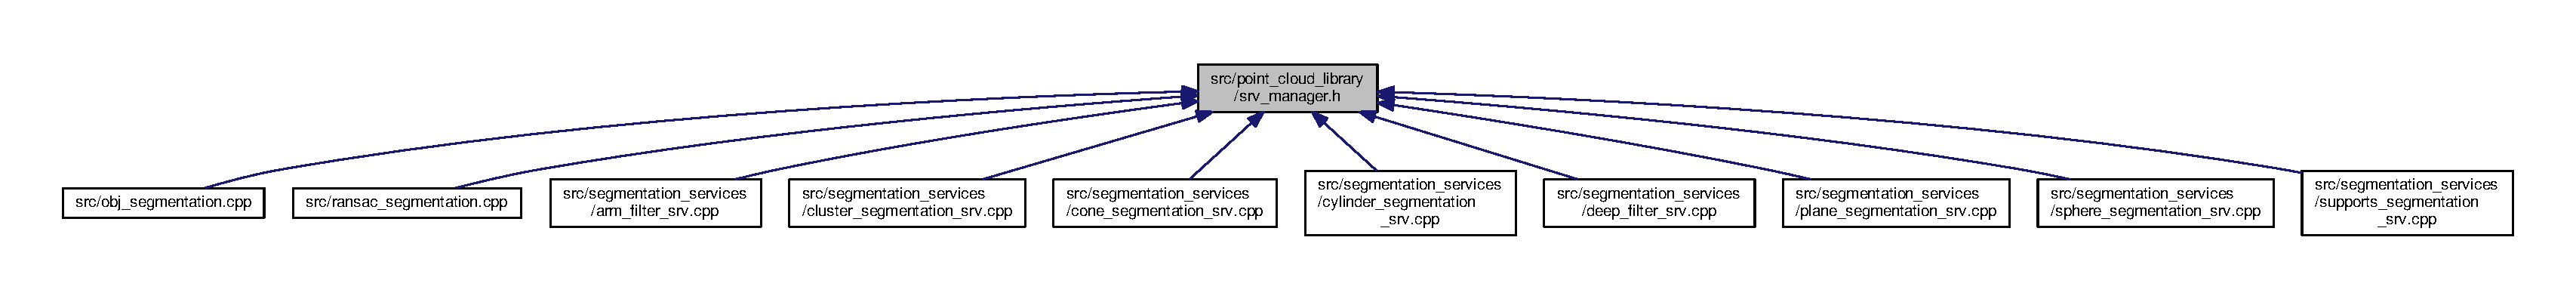
\includegraphics[width=350pt]{srv__manager_8h__dep__incl}
\end{center}
\end{figure}
\subsection*{Namespaces}
\begin{DoxyCompactItemize}
\item 
\hyperlink{namespacesrvm}{srvm}
\end{DoxyCompactItemize}
\subsection*{Functions}
\begin{DoxyCompactItemize}
\item 
const vector$<$ float $>$ \hyperlink{namespacesrvm_a78080cf77ae5d29a39ebcd3309b836fc}{srvm\-::\-D\-E\-F\-A\-U\-L\-T\-\_\-\-S\-E\-R\-V\-I\-C\-E\-\_\-\-V\-E\-C\-\_\-\-P\-A\-R\-A\-M\-E\-T\-E\-R\-\_\-\-R\-E\-Q\-U\-E\-S\-T} (D\-E\-F\-A\-U\-L\-T\-\_\-\-S\-E\-R\-V\-I\-C\-E\-\_\-\-A\-R\-R\-A\-Y\-\_\-\-P\-A\-R\-A\-M\-E\-T\-E\-R\-\_\-\-R\-E\-Q\-U\-E\-S\-T, D\-E\-F\-A\-U\-L\-T\-\_\-\-S\-E\-R\-V\-I\-C\-E\-\_\-\-A\-R\-R\-A\-Y\-\_\-\-P\-A\-R\-A\-M\-E\-T\-E\-R\-\_\-\-R\-E\-Q\-U\-E\-S\-T+sizeof(D\-E\-F\-A\-U\-L\-T\-\_\-\-S\-E\-R\-V\-I\-C\-E\-\_\-\-A\-R\-R\-A\-Y\-\_\-\-P\-A\-R\-A\-M\-E\-T\-E\-R\-\_\-\-R\-E\-Q\-U\-E\-S\-T)/sizeof(float))
\item 
string \hyperlink{namespacesrvm_a9c76ccfdb20b5ade1a837f4888a64997}{srvm\-::get\-String\-Parameter} (string input, const string default\-Value)
\item 
string \hyperlink{namespacesrvm_a2fe9c141c7827eaa0269319f179dfee5}{srvm\-::get\-String\-Ptr\-Parameter} (char $\ast$input, const string default\-Value)
\item 
bool \hyperlink{namespacesrvm_ac652beec1eacae6f527677f11e2a9256}{srvm\-::get\-Bool\-Parameter} (string input, const bool default\-Value)
\item 
bool \hyperlink{namespacesrvm_a4a300ace21cdfc4e753d7bbf97620f69}{srvm\-::get\-Bool\-Ptr\-Parameter} (char $\ast$input, const bool default\-Value)
\item 
string \hyperlink{namespacesrvm_a2d37598ea68edd23c273e90b7f544e85}{srvm\-::get\-Path\-Parameter} (string input, const string default\-Value)
\item 
string \hyperlink{namespacesrvm_acad80730421eaf35cda6c8dcb0c3b4d6}{srvm\-::get\-Path\-Ptr\-Parameter} (char $\ast$input, const string default\-Value)
\item 
float \hyperlink{namespacesrvm_ab17b035d854cf06a49bf869d1c23d76d}{srvm\-::get\-Service\-Float\-Parameter} (float input, const float default\-Value)
\item 
int \hyperlink{namespacesrvm_aca4253032e76670dd7e7b3c31fb59714}{srvm\-::get\-Service\-Int\-Parameter} (int input, const int default\-Value)
\item 
string \hyperlink{namespacesrvm_a26454c4e5c30136db86cb0aa0f5a91b0}{srvm\-::get\-Service\-String\-Parameter} (string input, const string default\-Value)
\item 
vector$<$ float $>$ \hyperlink{namespacesrvm_a40e6c519b06c6f44c4706e35ccd2b3dd}{srvm\-::get\-Service3\-D\-Array\-Parameter} (vector$<$ float $>$ input, const vector$<$ float $>$ default\-Value)
\item 
vector$<$ float $>$ \hyperlink{namespacesrvm_afd3f0061db924a7e0cbdfd06e2a7bb3c}{srvm\-::get3\-D\-Array} (const float values\mbox{[}$\,$\mbox{]})
\item 
vector$<$ float $>$ \hyperlink{namespacesrvm_a6fcb13a6186c7beda4a120b1a4f46313}{srvm\-::get\-Service3\-D\-Array\-Parameter} (vector$<$ float $>$ input, const float default\-Value\mbox{[}$\,$\mbox{]})
\item 
string \hyperlink{namespacesrvm_a0ceb768d016b217ced8c3d0b2a520862}{srvm\-::get\-Flag\-Value\-To\-Print} (bool flag)
\item 
string \hyperlink{namespacesrvm_a5796ceb6b857f7f21eb4f6056c251f00}{srvm\-::get\-Array\-To\-Print} (vector$<$ float $>$ arr)
\end{DoxyCompactItemize}
\subsection*{Variables}
\begin{DoxyCompactItemize}
\item 
const string \hyperlink{namespacesrvm_aef26ae8da6e703be7bbc1fc319fc18d5}{srvm\-::\-S\-R\-V\-\_\-\-N\-A\-M\-E\-\_\-\-D\-E\-E\-P\-\_\-\-F\-I\-L\-T\-E\-R} = \char`\"{}deep\-\_\-filter\-\_\-srv\char`\"{}
\item 
const string \hyperlink{namespacesrvm_a326e9454009b64e7e5bac20f050ff129}{srvm\-::\-S\-R\-V\-\_\-\-N\-A\-M\-E\-\_\-\-S\-U\-P\-P\-O\-R\-T\-\_\-\-F\-I\-L\-T\-E\-R} = \char`\"{}support\-\_\-segmentation\-\_\-srv\char`\"{}
\item 
const string \hyperlink{namespacesrvm_af1af7e755b5eb874d7bc4fec3d6585b2}{srvm\-::\-S\-R\-V\-\_\-\-N\-A\-M\-E\-\_\-\-C\-U\-S\-T\-E\-R\-\_\-\-F\-I\-L\-T\-E\-R} = \char`\"{}cluster\-\_\-\-Segmentation\-\_\-srv\char`\"{}
\item 
const string \hyperlink{namespacesrvm_ac0600b046091267fd4d0aed25786961f}{srvm\-::\-S\-R\-V\-\_\-\-N\-A\-M\-E\-\_\-\-A\-R\-M\-\_\-\-F\-I\-L\-T\-E\-R} = \char`\"{}arm\-\_\-filter\-\_\-srv\char`\"{}
\item 
const string \hyperlink{namespacesrvm_affa682d6f49c99cbf55802194970b5e5}{srvm\-::\-S\-R\-V\-\_\-\-N\-A\-M\-E\-\_\-\-R\-A\-N\-S\-A\-C\-\_\-\-S\-P\-H\-E\-R\-E\-\_\-\-F\-I\-L\-T\-E\-R} = \char`\"{}sphere\-\_\-segmentation\-\_\-srv\char`\"{}
\item 
const string \hyperlink{namespacesrvm_ae5db0900b3766ce489c65d143ae595b6}{srvm\-::\-S\-R\-V\-\_\-\-N\-A\-M\-E\-\_\-\-R\-A\-N\-S\-A\-C\-\_\-\-C\-Y\-L\-I\-N\-D\-E\-R\-\_\-\-F\-I\-L\-T\-E\-R} = \char`\"{}cylinder\-\_\-segmentation\-\_\-srv\char`\"{}
\item 
const string \hyperlink{namespacesrvm_af2812968f812d475d50a80635965779d}{srvm\-::\-S\-R\-V\-\_\-\-N\-A\-M\-E\-\_\-\-R\-A\-N\-S\-A\-C\-\_\-\-C\-O\-N\-E\-\_\-\-F\-I\-L\-T\-E\-R} = \char`\"{}cone\-\_\-segmentation\-\_\-srv\char`\"{}
\item 
const string \hyperlink{namespacesrvm_ab0f0109239fb85cfb303e5f44e4534f2}{srvm\-::\-S\-R\-V\-\_\-\-N\-A\-M\-E\-\_\-\-R\-A\-N\-S\-A\-C\-\_\-\-P\-L\-A\-N\-E\-\_\-\-F\-I\-L\-T\-E\-R} = \char`\"{}plane\-\_\-segmentation\-\_\-srv\char`\"{}
\item 
const string \hyperlink{namespacesrvm_ac5228e86d6d396c944b11f847746b3b8}{srvm\-::\-P\-A\-R\-A\-M\-\_\-\-N\-A\-M\-E\-\_\-\-I\-N\-P\-U\-T\-\_\-\-C\-L\-O\-U\-D\-\_\-\-R\-E\-F\-E\-R\-E\-N\-C\-E\-\_\-\-F\-R\-A\-M\-E} = \char`\"{}/pitt/ref\-\_\-frame/input\-\_\-cloud\char`\"{}
\item 
const string \hyperlink{namespacesrvm_a2984c458ad628e1230d49e4f1a3ee84a}{srvm\-::\-P\-A\-R\-A\-M\-\_\-\-N\-A\-M\-E\-\_\-\-O\-U\-T\-P\-U\-T\-\_\-\-C\-L\-O\-U\-D\-\_\-\-R\-E\-F\-E\-R\-E\-N\-C\-E\-\_\-\-F\-R\-A\-M\-E} = \char`\"{}/pitt/ref\-\_\-frame/output\-\_\-cloud\char`\"{}
\item 
const string \hyperlink{namespacesrvm_af5f0c98fe811a1ad130ec625e9b2cf75}{srvm\-::\-P\-A\-R\-A\-M\-\_\-\-N\-A\-M\-E\-\_\-\-D\-E\-E\-P\-\_\-\-S\-R\-V\-\_\-\-Z\-\_\-\-T\-H\-R\-E\-S\-H\-O\-L\-D} = \char`\"{}/pitt/service/deep\-\_\-filter/z\-\_\-threshold\char`\"{}
\item 
const string \hyperlink{namespacesrvm_a78229888a94a0362b2a4242a212e496f}{srvm\-::\-P\-A\-R\-A\-M\-\_\-\-N\-A\-M\-E\-\_\-\-A\-R\-M\-\_\-\-S\-R\-V\-\_\-\-M\-I\-N\-\_\-\-F\-O\-R\-E\-A\-R\-M\-\_\-\-B\-O\-X} = \char`\"{}/pitt/srv/arm\-\_\-filter/min\-\_\-forearm\-\_\-box\char`\"{}
\item 
const string \hyperlink{namespacesrvm_a566bcfbd837fb5450a2c9c6de09d522a}{srvm\-::\-P\-A\-R\-A\-M\-\_\-\-N\-A\-M\-E\-\_\-\-A\-R\-M\-\_\-\-S\-R\-V\-\_\-\-M\-A\-X\-\_\-\-F\-O\-R\-E\-A\-R\-M\-\_\-\-B\-O\-X} = \char`\"{}/pitt/srv/arm\-\_\-filter/max\-\_\-forearm\-\_\-box\char`\"{}
\item 
const string \hyperlink{namespacesrvm_ae85ac94c938b94bb075b175237d198b0}{srvm\-::\-P\-A\-R\-A\-M\-\_\-\-N\-A\-M\-E\-\_\-\-A\-R\-M\-\_\-\-S\-R\-V\-\_\-\-M\-I\-N\-\_\-\-E\-L\-B\-O\-W\-\_\-\-B\-O\-X} = \char`\"{}/pitt/srv/arm\-\_\-filter/min\-\_\-elbow\-\_\-box\char`\"{}
\item 
const string \hyperlink{namespacesrvm_afeb3197fee2f13444309f3e4ed314392}{srvm\-::\-P\-A\-R\-A\-M\-\_\-\-N\-A\-M\-E\-\_\-\-A\-R\-M\-\_\-\-S\-R\-V\-\_\-\-M\-A\-X\-\_\-\-E\-L\-B\-O\-W\-\_\-\-B\-O\-X} = \char`\"{}/pitt/srv/arm\-\_\-filter/max\-\_\-elbow\-\_\-box\char`\"{}
\item 
const string \hyperlink{namespacesrvm_a606c20312640e9cc8710e4d43f0cb167}{srvm\-::\-P\-A\-R\-A\-M\-\_\-\-N\-A\-M\-E\-\_\-\-C\-L\-U\-S\-T\-E\-R\-\_\-\-T\-O\-L\-E\-R\-A\-N\-C\-E} = \char`\"{}/pitt/srv/cluster\-\_\-segmentation/tolerance\char`\"{}
\item 
const string \hyperlink{namespacesrvm_a68216326c13293ff70084f03bb4efa98}{srvm\-::\-P\-A\-R\-A\-M\-\_\-\-N\-A\-M\-E\-\_\-\-C\-L\-U\-S\-T\-E\-R\-\_\-\-M\-I\-N\-\_\-\-R\-A\-T\-E} = \char`\"{}/pitt/srv/cluster\-\_\-segmentation/min\-\_\-rate\char`\"{}
\item 
const string \hyperlink{namespacesrvm_ac57a3b8f3addc024383db76f1d2c55da}{srvm\-::\-P\-A\-R\-A\-M\-\_\-\-N\-A\-M\-E\-\_\-\-C\-L\-U\-S\-T\-E\-R\-\_\-\-M\-A\-X\-\_\-\-R\-A\-T\-E} = \char`\"{}/pitt/srv/cluster\-\_\-segmentation/max\-\_\-rate\char`\"{}
\item 
const string \hyperlink{namespacesrvm_a3f21a743638bc9a2a5fbfbc5711e4095}{srvm\-::\-P\-A\-R\-A\-M\-\_\-\-N\-A\-M\-E\-\_\-\-C\-L\-U\-S\-T\-E\-R\-\_\-\-M\-I\-N\-\_\-\-I\-N\-P\-U\-T\-\_\-\-S\-I\-Z\-E} = \char`\"{}/pitt/srv/cluster\-\_\-segmentation/min\-\_\-input\-\_\-size\char`\"{}
\item 
const string \hyperlink{namespacesrvm_ae88e28586870382fc0b407646869f0c4}{srvm\-::\-P\-A\-R\-A\-M\-\_\-\-N\-A\-M\-E\-\_\-\-S\-P\-H\-E\-R\-E\-\_\-\-N\-O\-R\-M\-A\-L\-\_\-\-D\-I\-S\-T\-A\-N\-C\-E\-\_\-\-W\-E\-I\-G\-H\-T} = \char`\"{}/pitt/srv/sphere\-\_\-segmentation/normal\-\_\-distance\-\_\-weight\char`\"{}
\item 
const string \hyperlink{namespacesrvm_aacb054d1f0139845cf32c294b210b96c}{srvm\-::\-P\-A\-R\-A\-M\-\_\-\-N\-A\-M\-E\-\_\-\-S\-P\-H\-E\-R\-E\-\_\-\-D\-I\-S\-T\-A\-N\-C\-E\-\_\-\-T\-H} = \char`\"{}/pitt/srv/sphere\-\_\-segmentation/distance\-\_\-th\char`\"{}
\item 
const string \hyperlink{namespacesrvm_a098cc851c26290df58470c9287263f76}{srvm\-::\-P\-A\-R\-A\-M\-\_\-\-N\-A\-M\-E\-\_\-\-S\-P\-H\-E\-R\-E\-\_\-\-M\-A\-X\-\_\-\-I\-T\-E\-R\-A\-T\-I\-O\-N\-\_\-\-L\-I\-M\-I\-T} = \char`\"{}/pitt/srv/sphere\-\_\-segmentation/max\-\_\-iter\-\_\-limit\char`\"{}
\item 
const string \hyperlink{namespacesrvm_aba736b64edcfd2a08ed56065f94d7e71}{srvm\-::\-P\-A\-R\-A\-M\-\_\-\-N\-A\-M\-E\-\_\-\-S\-P\-H\-E\-R\-E\-\_\-\-M\-I\-N\-\_\-\-R\-A\-D\-I\-U\-S\-\_\-\-L\-I\-M\-I\-T} = \char`\"{}/pitt/srv/sphere\-\_\-segmentation/min\-\_\-radius\-\_\-limit\char`\"{}
\item 
const string \hyperlink{namespacesrvm_ac79f9145796395f45f9c06cefc6876aa}{srvm\-::\-P\-A\-R\-A\-M\-\_\-\-N\-A\-M\-E\-\_\-\-S\-P\-H\-E\-R\-E\-\_\-\-M\-A\-X\-\_\-\-R\-A\-D\-I\-U\-S\-\_\-\-L\-I\-M\-I\-T} = \char`\"{}/pitt/srv/sphere\-\_\-segmentation/max\-\_\-radius\-\_\-limit\char`\"{}
\item 
const string \hyperlink{namespacesrvm_aac6381551a69b2d103ccdb9aeefcfa1d}{srvm\-::\-P\-A\-R\-A\-M\-\_\-\-N\-A\-M\-E\-\_\-\-S\-P\-H\-E\-R\-E\-\_\-\-E\-P\-S\-\_\-\-A\-N\-G\-L\-E\-\_\-\-T\-H} = \char`\"{}/pitt/srv/sphere\-\_\-segmentation/eps\-\_\-angle\-\_\-th\char`\"{}
\item 
const string \hyperlink{namespacesrvm_a5a4d80e9cdfeb1e4a0e28c58b3ad40af}{srvm\-::\-P\-A\-R\-A\-M\-\_\-\-N\-A\-M\-E\-\_\-\-S\-P\-H\-E\-R\-E\-\_\-\-M\-I\-N\-\_\-\-O\-P\-E\-N\-I\-N\-G\-\_\-\-A\-N\-G\-L\-E\-\_\-\-D\-E\-G\-R\-E\-E} = \char`\"{}/pitt/srv/sphere\-\_\-segmentation/min\-\_\-opening\-\_\-angle\-\_\-deg\char`\"{}
\item 
const string \hyperlink{namespacesrvm_ae8a655418ddc4f96bc9a13d245a5dafb}{srvm\-::\-P\-A\-R\-A\-M\-\_\-\-N\-A\-M\-E\-\_\-\-S\-P\-H\-E\-R\-E\-\_\-\-M\-A\-X\-\_\-\-O\-P\-E\-N\-I\-N\-G\-\_\-\-A\-N\-G\-L\-E\-\_\-\-D\-E\-G\-R\-E\-E} = \char`\"{}/pitt/srv/sphere\-\_\-segmentation/max\-\_\-opening\-\_\-angle\-\_\-deg\char`\"{}
\item 
const string \hyperlink{namespacesrvm_a3c779659d33a4785a807abe53c2bf52f}{srvm\-::\-P\-A\-R\-A\-M\-\_\-\-N\-A\-M\-E\-\_\-\-S\-P\-H\-E\-R\-E\-\_\-\-M\-I\-N\-\_\-\-I\-N\-L\-I\-E\-R\-S} = \char`\"{}/pitt/srv/sphere\-\_\-segmentation/min\-\_\-inliers\char`\"{}
\item 
const string \hyperlink{namespacesrvm_a09193d91d1605cb57a465191c5c76937}{srvm\-::\-P\-A\-R\-A\-M\-\_\-\-N\-A\-M\-E\-\_\-\-C\-Y\-L\-I\-N\-D\-E\-R\-\_\-\-N\-O\-R\-M\-A\-L\-\_\-\-D\-I\-S\-T\-A\-N\-C\-E\-\_\-\-W\-E\-I\-G\-H\-T} = \char`\"{}/pitt/srv/cylinder\-\_\-segmentation/normal\-\_\-distance\-\_\-weight\char`\"{}
\item 
const string \hyperlink{namespacesrvm_a5c4d574f82749332080a69b24f701293}{srvm\-::\-P\-A\-R\-A\-M\-\_\-\-N\-A\-M\-E\-\_\-\-C\-Y\-L\-I\-N\-D\-E\-R\-\_\-\-D\-I\-S\-T\-A\-N\-C\-E\-\_\-\-T\-H} = \char`\"{}/pitt/srv/cylinder\-\_\-segmentation/distance\-\_\-th\char`\"{}
\item 
const string \hyperlink{namespacesrvm_a6014be265a0226940dadfd3dbab61ddd}{srvm\-::\-P\-A\-R\-A\-M\-\_\-\-N\-A\-M\-E\-\_\-\-C\-Y\-L\-I\-N\-D\-E\-R\-\_\-\-M\-A\-X\-\_\-\-I\-T\-E\-R\-A\-T\-I\-O\-N\-\_\-\-L\-I\-M\-I\-T} = \char`\"{}/pitt/srv/cylinder\-\_\-segmentation/max\-\_\-iter\-\_\-limit\char`\"{}
\item 
const string \hyperlink{namespacesrvm_ab1881c1282b48afac271ea14a806c34f}{srvm\-::\-P\-A\-R\-A\-M\-\_\-\-N\-A\-M\-E\-\_\-\-C\-Y\-L\-I\-N\-D\-E\-R\-\_\-\-M\-I\-N\-\_\-\-R\-A\-D\-I\-U\-S\-\_\-\-L\-I\-M\-I\-T} = \char`\"{}/pitt/srv/cylinder\-\_\-segmentation/min\-\_\-radius\-\_\-limit\char`\"{}
\item 
const string \hyperlink{namespacesrvm_a85b64ea120e2c925a89075ad4efce82a}{srvm\-::\-P\-A\-R\-A\-M\-\_\-\-N\-A\-M\-E\-\_\-\-C\-Y\-L\-I\-N\-D\-E\-R\-\_\-\-M\-A\-X\-\_\-\-R\-A\-D\-I\-U\-S\-\_\-\-L\-I\-M\-I\-T} = \char`\"{}/pitt/srv/cylinder\-\_\-segmentation/max\-\_\-radius\-\_\-limit\char`\"{}
\item 
const string \hyperlink{namespacesrvm_a7e9ad3e08d4a3bca5694b38a5fb4a3f7}{srvm\-::\-P\-A\-R\-A\-M\-\_\-\-N\-A\-M\-E\-\_\-\-C\-Y\-L\-I\-N\-D\-E\-R\-\_\-\-E\-P\-S\-\_\-\-A\-N\-G\-L\-E\-\_\-\-T\-H} = \char`\"{}/pitt/srv/cylinder\-\_\-segmentation/eps\-\_\-angle\-\_\-th\char`\"{}
\item 
const string \hyperlink{namespacesrvm_a3033f0baf12b9ba742cbb14be2f9516b}{srvm\-::\-P\-A\-R\-A\-M\-\_\-\-N\-A\-M\-E\-\_\-\-C\-Y\-L\-I\-N\-D\-E\-R\-\_\-\-M\-I\-N\-\_\-\-O\-P\-E\-N\-I\-N\-G\-\_\-\-A\-N\-G\-L\-E\-\_\-\-D\-E\-G\-R\-E\-E} = \char`\"{}/pitt/srv/cylinder\-\_\-segmentation/min\-\_\-opening\-\_\-angle\-\_\-deg\char`\"{}
\item 
const string \hyperlink{namespacesrvm_ae8a34e53f1f93958a83db46e8b57b4f0}{srvm\-::\-P\-A\-R\-A\-M\-\_\-\-N\-A\-M\-E\-\_\-\-C\-Y\-L\-I\-N\-D\-E\-R\-\_\-\-M\-A\-X\-\_\-\-O\-P\-E\-N\-I\-N\-G\-\_\-\-A\-N\-G\-L\-E\-\_\-\-D\-E\-G\-R\-E\-E} = \char`\"{}/pitt/srv/cylinder\-\_\-segmentation/max\-\_\-opening\-\_\-angle\-\_\-deg\char`\"{}
\item 
const string \hyperlink{namespacesrvm_a1cf16bab1dafeefe6d5f6a58432ecbc0}{srvm\-::\-P\-A\-R\-A\-M\-\_\-\-N\-A\-M\-E\-\_\-\-C\-Y\-L\-I\-N\-D\-E\-R\-\_\-\-M\-I\-N\-\_\-\-I\-N\-L\-I\-E\-R\-S} = \char`\"{}/pitt/srv/cylinder\-\_\-segmentation/min\-\_\-inliers\char`\"{}
\item 
const string \hyperlink{namespacesrvm_a6d02fc836a0b8eb1e6cd8a03e12758d7}{srvm\-::\-P\-A\-R\-A\-M\-\_\-\-N\-A\-M\-E\-\_\-\-C\-O\-N\-E\-\_\-\-N\-O\-R\-M\-A\-L\-\_\-\-D\-I\-S\-T\-A\-N\-C\-E\-\_\-\-W\-E\-I\-G\-H\-T} = \char`\"{}/pitt/srv/cone\-\_\-segmentation/normal\-\_\-distance\-\_\-weight\char`\"{}
\item 
const string \hyperlink{namespacesrvm_aeec863664b339e3c4808736477fe1378}{srvm\-::\-P\-A\-R\-A\-M\-\_\-\-N\-A\-M\-E\-\_\-\-C\-O\-N\-E\-\_\-\-D\-I\-S\-T\-A\-N\-C\-E\-\_\-\-T\-H} = \char`\"{}/pitt/srv/cone\-\_\-segmentation/distance\-\_\-th\char`\"{}
\item 
const string \hyperlink{namespacesrvm_a247e146bdc00ad4dc26a1b521b3eb53b}{srvm\-::\-P\-A\-R\-A\-M\-\_\-\-N\-A\-M\-E\-\_\-\-C\-O\-N\-E\-\_\-\-M\-A\-X\-\_\-\-I\-T\-E\-R\-A\-T\-I\-O\-N\-\_\-\-L\-I\-M\-I\-T} = \char`\"{}/pitt/srv/cone\-\_\-segmentation/max\-\_\-iter\-\_\-limit\char`\"{}
\item 
const string \hyperlink{namespacesrvm_a2d22b702cf298b11c0a70ab4fa90555e}{srvm\-::\-P\-A\-R\-A\-M\-\_\-\-N\-A\-M\-E\-\_\-\-C\-O\-N\-E\-\_\-\-M\-I\-N\-\_\-\-R\-A\-D\-I\-U\-S\-\_\-\-L\-I\-M\-I\-T} = \char`\"{}/pitt/srv/cone\-\_\-segmentation/min\-\_\-radius\-\_\-limit\char`\"{}
\item 
const string \hyperlink{namespacesrvm_a684755d042c9407cf88fcc81ca6a5712}{srvm\-::\-P\-A\-R\-A\-M\-\_\-\-N\-A\-M\-E\-\_\-\-C\-O\-N\-E\-\_\-\-M\-A\-X\-\_\-\-R\-A\-D\-I\-U\-S\-\_\-\-L\-I\-M\-I\-T} = \char`\"{}/pitt/srv/cone\-\_\-segmentation/max\-\_\-radius\-\_\-limit\char`\"{}
\item 
const string \hyperlink{namespacesrvm_a6023448f3a02902eec73727de0699571}{srvm\-::\-P\-A\-R\-A\-M\-\_\-\-N\-A\-M\-E\-\_\-\-C\-O\-N\-E\-\_\-\-E\-P\-S\-\_\-\-A\-N\-G\-L\-E\-\_\-\-T\-H} = \char`\"{}/pitt/srv/cone\-\_\-segmentation/eps\-\_\-angle\-\_\-th\char`\"{}
\item 
const string \hyperlink{namespacesrvm_aeee569608876be7a3b9c7deb18037aeb}{srvm\-::\-P\-A\-R\-A\-M\-\_\-\-N\-A\-M\-E\-\_\-\-C\-O\-N\-E\-\_\-\-M\-I\-N\-\_\-\-O\-P\-E\-N\-I\-N\-G\-\_\-\-A\-N\-G\-L\-E\-\_\-\-D\-E\-G\-R\-E\-E} = \char`\"{}/pitt/srv/cone\-\_\-segmentation/min\-\_\-opening\-\_\-angle\-\_\-deg\char`\"{}
\item 
const string \hyperlink{namespacesrvm_acfa6baa980590edd027af05d215e92f4}{srvm\-::\-P\-A\-R\-A\-M\-\_\-\-N\-A\-M\-E\-\_\-\-C\-O\-N\-E\-\_\-\-M\-A\-X\-\_\-\-O\-P\-E\-N\-I\-N\-G\-\_\-\-A\-N\-G\-L\-E\-\_\-\-D\-E\-G\-R\-E\-E} = \char`\"{}/pitt/srv/cone\-\_\-segmentation/max\-\_\-opening\-\_\-angle\-\_\-deg\char`\"{}
\item 
const string \hyperlink{namespacesrvm_a228bc70cd1578c12026757a28b369ea1}{srvm\-::\-P\-A\-R\-A\-M\-\_\-\-N\-A\-M\-E\-\_\-\-C\-O\-N\-E\-\_\-\-M\-I\-N\-\_\-\-I\-N\-L\-I\-E\-R\-S} = \char`\"{}/pitt/srv/cone\-\_\-segmentation/min\-\_\-inliers\char`\"{}
\item 
const string \hyperlink{namespacesrvm_aa92c5d3af4d21e544d422eb317a4558d}{srvm\-::\-P\-A\-R\-A\-M\-\_\-\-N\-A\-M\-E\-\_\-\-P\-L\-A\-N\-E\-\_\-\-N\-O\-R\-M\-A\-L\-\_\-\-D\-I\-S\-T\-A\-N\-C\-E\-\_\-\-W\-E\-I\-G\-H\-T} = \char`\"{}/pitt/srv/plane\-\_\-segmentation/normal\-\_\-distance\-\_\-weight\char`\"{}
\item 
const string \hyperlink{namespacesrvm_afdcd3222bf4aee9b48f2eb9f56b496e5}{srvm\-::\-P\-A\-R\-A\-M\-\_\-\-N\-A\-M\-E\-\_\-\-P\-L\-A\-N\-E\-\_\-\-D\-I\-S\-T\-A\-N\-C\-E\-\_\-\-T\-H} = \char`\"{}/pitt/srv/plane\-\_\-segmentation/distance\-\_\-th\char`\"{}
\item 
const string \hyperlink{namespacesrvm_a64f33d61b5b06a55234199642e8db783}{srvm\-::\-P\-A\-R\-A\-M\-\_\-\-N\-A\-M\-E\-\_\-\-P\-L\-A\-N\-E\-\_\-\-M\-A\-X\-\_\-\-I\-T\-E\-R\-A\-T\-I\-O\-N\-\_\-\-L\-I\-M\-I\-T} = \char`\"{}/pitt/srv/plane\-\_\-segmentation/max\-\_\-iter\-\_\-limit\char`\"{}
\item 
const string \hyperlink{namespacesrvm_a2a1ca687f68863e4c300c2cd269c53ac}{srvm\-::\-P\-A\-R\-A\-M\-\_\-\-N\-A\-M\-E\-\_\-\-P\-L\-A\-N\-E\-\_\-\-E\-P\-S\-\_\-\-A\-N\-G\-L\-E\-\_\-\-T\-H} = \char`\"{}/pitt/srv/plane\-\_\-segmentation/eps\-\_\-angle\-\_\-th\char`\"{}
\item 
const string \hyperlink{namespacesrvm_a31fdf967c804692f260cf6ec8e219232}{srvm\-::\-P\-A\-R\-A\-M\-\_\-\-N\-A\-M\-E\-\_\-\-P\-L\-A\-N\-E\-\_\-\-M\-I\-N\-\_\-\-O\-P\-E\-N\-I\-N\-G\-\_\-\-A\-N\-G\-L\-E\-\_\-\-D\-E\-G\-R\-E\-E} = \char`\"{}/pitt/srv/plane\-\_\-segmentation/min\-\_\-opening\-\_\-angle\-\_\-deg\char`\"{}
\item 
const string \hyperlink{namespacesrvm_a22f7d6b9a304a08f863e8a0c0084b2f2}{srvm\-::\-P\-A\-R\-A\-M\-\_\-\-N\-A\-M\-E\-\_\-\-P\-L\-A\-N\-E\-\_\-\-M\-A\-X\-\_\-\-O\-P\-E\-N\-I\-N\-G\-\_\-\-A\-N\-G\-L\-E\-\_\-\-D\-E\-G\-R\-E\-E} = \char`\"{}/pitt/srv/plane\-\_\-segmentation/max\-\_\-opening\-\_\-angle\-\_\-deg\char`\"{}
\item 
const string \hyperlink{namespacesrvm_a279d85c7afac2390d2552ae90cd4ea05}{srvm\-::\-P\-A\-R\-A\-M\-\_\-\-N\-A\-M\-E\-\_\-\-P\-L\-A\-N\-E\-\_\-\-M\-I\-N\-\_\-\-I\-N\-L\-I\-E\-R\-S} = \char`\"{}/pitt/srv/plane\-\_\-segmentation/min\-\_\-inliers\char`\"{}
\item 
const string \hyperlink{namespacesrvm_ac6d56e59d27ae79b392d58c0b57d03e1}{srvm\-::\-P\-A\-R\-A\-M\-\_\-\-N\-A\-M\-E\-\_\-\-M\-I\-N\-\_\-\-I\-T\-E\-R\-A\-T\-I\-V\-E\-\_\-\-C\-L\-O\-U\-D\-\_\-\-P\-E\-R\-C\-E\-N\-T\-A\-G\-E} = \char`\"{}/pitt/srv/supports\-\_\-segmentation/min\-\_\-iter\-\_\-cloud\-\_\-percent\char`\"{}
\item 
const string \hyperlink{namespacesrvm_a209e7ad2de58ec5193770fc4d9cd98ab}{srvm\-::\-P\-A\-R\-A\-M\-\_\-\-N\-A\-M\-E\-\_\-\-M\-I\-N\-\_\-\-I\-T\-E\-R\-A\-T\-I\-V\-E\-\_\-\-S\-U\-P\-P\-O\-R\-T\-\_\-\-P\-E\-R\-C\-E\-N\-T\-A\-G\-E} = \char`\"{}/pitt/srv/supports\-\_\-segmentation/min\-\_\-iter\-\_\-support\-\_\-percent\char`\"{}
\item 
const string \hyperlink{namespacesrvm_adb071b5e180a1109af154bd4241a250e}{srvm\-::\-P\-A\-R\-A\-M\-\_\-\-N\-A\-M\-E\-\_\-\-H\-O\-R\-I\-Z\-O\-N\-T\-A\-L\-\_\-\-V\-A\-R\-I\-A\-N\-C\-E\-\_\-\-T\-H\-R\-E\-S\-H\-O\-L\-D} = \char`\"{}/pitt/srv/supports\-\_\-segmentation/horizontal\-\_\-variance\-\_\-th\char`\"{}
\item 
const string \hyperlink{namespacesrvm_af1a83a2964c2f60f7f497f05ef454cfd}{srvm\-::\-P\-A\-R\-A\-M\-\_\-\-N\-A\-M\-E\-\_\-\-R\-A\-N\-S\-A\-C\-\_\-\-I\-N\-\_\-\-S\-H\-A\-P\-E\-\_\-\-D\-I\-S\-T\-A\-N\-C\-E\-\_\-\-P\-O\-I\-N\-T\-\_\-\-T\-H\-R\-E\-S\-H\-O\-L\-D} = \char`\"{}/pitt/srv/supports\-\_\-segmentation/in\-\_\-shape\-\_\-distance\-\_\-th\char`\"{}
\item 
const string \hyperlink{namespacesrvm_ad592efae9026788849614a69053f3914}{srvm\-::\-P\-A\-R\-A\-M\-\_\-\-N\-A\-M\-E\-\_\-\-R\-A\-N\-S\-A\-C\-\_\-\-M\-O\-D\-E\-L\-\_\-\-N\-O\-R\-M\-A\-L\-\_\-\-D\-I\-S\-T\-A\-N\-C\-E\-\_\-\-W\-E\-I\-G\-H\-T} = \char`\"{}/pitt/srv/supports\-\_\-segmentation/normal\-\_\-distance\-\_\-weight\char`\"{}
\item 
const string \hyperlink{namespacesrvm_aa6b5f05b01cb661c1481c0f40bd916e4}{srvm\-::\-P\-A\-R\-A\-M\-\_\-\-N\-A\-M\-E\-\_\-\-R\-A\-N\-S\-A\-C\-\_\-\-M\-A\-X\-\_\-\-I\-T\-E\-R\-A\-T\-I\-O\-N\-\_\-\-T\-H\-R\-E\-S\-H\-O\-L\-D} = \char`\"{}/pitt/srv/supports\-\_\-segmentation/max\-\_\-iter\char`\"{}
\item 
const string \hyperlink{namespacesrvm_a2957bf6ee16944664364c470f1beb958}{srvm\-::\-P\-A\-R\-A\-M\-\_\-\-N\-A\-M\-E\-\_\-\-H\-O\-R\-I\-Z\-O\-N\-T\-A\-L\-\_\-\-A\-X\-I\-S} = \char`\"{}/pitt/srv/supports\-\_\-segmentation/horizontal\-\_\-axis\char`\"{}
\item 
const string \hyperlink{namespacesrvm_a07211b3f36f93931af6e67097b75f145}{srvm\-::\-P\-A\-R\-A\-M\-\_\-\-N\-A\-M\-E\-\_\-\-S\-U\-P\-P\-O\-R\-T\-\_\-\-E\-D\-G\-E\-\_\-\-R\-E\-M\-O\-V\-E\-\_\-\-O\-F\-F\-S\-E\-T} = \char`\"{}/pitt/srv/supports\-\_\-segmentation/edge\-\_\-remove\-\_\-offset\char`\"{}
\item 
const string \hyperlink{namespacesrvm_a2c4c31d893bfef55ede38ab56f4e7658}{srvm\-::\-D\-E\-F\-A\-U\-L\-T\-\_\-\-P\-A\-R\-A\-M\-\_\-\-I\-N\-P\-U\-T\-\_\-\-C\-L\-O\-U\-D\-\_\-\-R\-E\-F\-E\-R\-E\-N\-C\-E\-\_\-\-F\-R\-A\-M\-E} = \char`\"{}/camera\-\_\-depth\-\_\-optical\-\_\-frame\char`\"{}
\item 
const string \hyperlink{namespacesrvm_a228565e6d2ec6f457f78c4412d6c7daa}{srvm\-::\-D\-E\-F\-A\-U\-L\-T\-\_\-\-P\-A\-R\-A\-M\-\_\-\-O\-U\-T\-P\-U\-T\-\_\-\-C\-L\-O\-U\-D\-\_\-\-R\-E\-F\-E\-R\-E\-N\-C\-E\-\_\-\-F\-R\-A\-M\-E} = \char`\"{}/world\char`\"{}
\item 
const string \hyperlink{namespacesrvm_afb9bab9dced618a8992cf505cf484b1c}{srvm\-::\-D\-E\-F\-A\-U\-L\-T\-\_\-\-I\-N\-P\-U\-T\-\_\-\-P\-A\-R\-A\-M\-\_\-\-R\-A\-W\-\_\-\-C\-L\-O\-U\-D\-\_\-\-T\-O\-P\-I\-C} = \char`\"{}/camera/depth/points\char`\"{}
\item 
const string \hyperlink{namespacesrvm_a92921b8b79655fa69a697a54dca42056}{srvm\-::\-D\-E\-F\-A\-U\-L\-T\-\_\-\-I\-N\-P\-U\-T\-\_\-\-P\-A\-R\-A\-M\-\_\-\-C\-E\-N\-T\-R\-O\-I\-D\-\_\-\-L\-O\-G\-\_\-\-F\-I\-L\-E} = \char`\"{}\char`\"{}
\item 
const bool \hyperlink{namespacesrvm_ac54afc31491c977345ef1a1fbb563be3}{srvm\-::\-D\-E\-F\-A\-U\-L\-T\-\_\-\-I\-N\-P\-U\-T\-\_\-\-P\-A\-R\-A\-M\-\_\-\-S\-H\-O\-W\-\_\-\-O\-R\-I\-G\-I\-N\-A\-L\-\_\-\-C\-L\-O\-U\-D} = false
\item 
const bool \hyperlink{namespacesrvm_a9880144ef0df953c3b583e4f20dbff76}{srvm\-::\-D\-E\-F\-A\-U\-L\-T\-\_\-\-I\-N\-P\-U\-T\-\_\-\-P\-A\-R\-A\-M\-\_\-\-S\-H\-O\-W\-\_\-\-S\-U\-P\-P\-O\-R\-T\-S} = false
\item 
const bool \hyperlink{namespacesrvm_a8e6760e3e9557fc2fb87cbb6fcd8b3e6}{srvm\-::\-D\-E\-F\-A\-U\-L\-T\-\_\-\-I\-N\-P\-U\-T\-\_\-\-P\-A\-R\-A\-M\-\_\-\-S\-H\-O\-W\-\_\-\-O\-B\-J\-E\-C\-T\-\_\-\-O\-N\-\_\-\-S\-U\-P\-P\-O\-R\-T} = false
\item 
const bool \hyperlink{namespacesrvm_aef053199a3f95b1da712ef187b096f93}{srvm\-::\-D\-E\-F\-A\-U\-L\-T\-\_\-\-I\-N\-P\-U\-T\-\_\-\-P\-A\-R\-A\-M\-\_\-\-S\-H\-O\-W\-\_\-\-C\-L\-U\-S\-T\-E\-R\-S} = false
\item 
const string \hyperlink{namespacesrvm_a9ae9e53a20ec9335fe07c1a42520198e}{srvm\-::\-D\-E\-F\-A\-U\-L\-T\-\_\-\-P\-A\-R\-A\-M\-\_\-\-A\-R\-M\-\_\-\-S\-R\-V\-\_\-\-C\-A\-M\-E\-R\-A\-\_\-\-F\-R\-A\-M\-E} = \char`\"{}/camera\-\_\-depth\-\_\-optical\-\_\-frame\char`\"{}
\item 
const string \hyperlink{namespacesrvm_a6e203b3aafd97558c58ada022c9cc514}{srvm\-::\-D\-E\-F\-A\-U\-L\-T\-\_\-\-P\-A\-R\-A\-M\-\_\-\-A\-R\-M\-\_\-\-S\-R\-V\-\_\-\-R\-I\-G\-H\-T\-\_\-\-F\-O\-R\-E\-A\-R\-M\-\_\-\-F\-R\-A\-M\-E} = \char`\"{}/right\-\_\-lower\-\_\-forearm\char`\"{}
\item 
const string \hyperlink{namespacesrvm_af63966bf248ec14ccf2a2ca74fa1214d}{srvm\-::\-D\-E\-F\-A\-U\-L\-T\-\_\-\-P\-A\-R\-A\-M\-\_\-\-A\-R\-M\-\_\-\-S\-R\-V\-\_\-\-L\-E\-F\-T\-\_\-\-F\-O\-R\-E\-A\-R\-M\-\_\-\-F\-R\-A\-M\-E} = \char`\"{}/left\-\_\-lower\-\_\-forearm\char`\"{}
\item 
const string \hyperlink{namespacesrvm_acb12c9f4a5661db79a05ea222c83e215}{srvm\-::\-D\-E\-F\-A\-U\-L\-T\-\_\-\-P\-A\-R\-A\-M\-\_\-\-A\-R\-M\-\_\-\-S\-R\-V\-\_\-\-R\-I\-G\-H\-T\-\_\-\-E\-L\-B\-O\-W\-\_\-\-F\-R\-A\-M\-E} = \char`\"{}/right\-\_\-lower\-\_\-elbow\char`\"{}
\item 
const string \hyperlink{namespacesrvm_ab8271bafa5b004c13196b24b77cef53a}{srvm\-::\-D\-E\-F\-A\-U\-L\-T\-\_\-\-P\-A\-R\-A\-M\-\_\-\-A\-R\-M\-\_\-\-S\-R\-V\-\_\-\-L\-E\-F\-T\-\_\-\-E\-L\-B\-O\-W\-\_\-\-F\-R\-A\-M\-E} = \char`\"{}/left\-\_\-lower\-\_\-elbow\char`\"{}
\item 
const bool \hyperlink{namespacesrvm_a7fdc748a5c9f8f7211d6e32e64f96c63}{srvm\-::\-D\-E\-F\-A\-U\-L\-T\-\_\-\-P\-A\-R\-A\-M\-\_\-\-A\-R\-M\-\_\-\-S\-R\-V\-\_\-\-S\-H\-O\-W\-\_\-\-C\-L\-O\-U\-D\-S} = false
\item 
const string \hyperlink{namespacesrvm_a520b8813dc65ba764d59f05a0b316e5c}{srvm\-::\-T\-O\-P\-I\-C\-\_\-\-O\-U\-T\-\_\-\-N\-A\-M\-E\-\_\-\-O\-B\-J\-E\-C\-T\-\_\-\-P\-E\-R\-C\-E\-P\-T\-I\-O\-N} = \char`\"{}obj\-\_\-segmentation/Cluster\-Output\char`\"{}
\item 
const int \hyperlink{namespacesrvm_a27b2693a98ba8791767e3c8bebdab105}{srvm\-::\-D\-E\-F\-A\-U\-L\-T\-\_\-\-S\-E\-R\-V\-I\-C\-E\-\_\-\-P\-A\-R\-A\-M\-E\-T\-E\-R\-\_\-\-R\-E\-Q\-U\-E\-S\-T} = -\/1
\item 
const float \hyperlink{namespacesrvm_a5a9ae08c1a139bbf76b39c5d34f90e2a}{srvm\-::\-D\-E\-F\-A\-U\-L\-T\-\_\-\-S\-E\-R\-V\-I\-C\-E\-\_\-\-P\-A\-R\-A\-M\-E\-T\-E\-R\-\_\-\-R\-E\-Q\-U\-E\-S\-T\-\_\-\-F} = -\/1.\-0f
\item 
const float \hyperlink{namespacesrvm_a07324815e3638c6740336e50699d3300}{srvm\-::\-D\-E\-F\-A\-U\-L\-T\-\_\-\-S\-E\-R\-V\-I\-C\-E\-\_\-\-A\-R\-R\-A\-Y\-\_\-\-P\-A\-R\-A\-M\-E\-T\-E\-R\-\_\-\-R\-E\-Q\-U\-E\-S\-T} \mbox{[}1\mbox{]} = \{-\/1\}
\item 
const float \hyperlink{namespacesrvm_a6debc60d19f8c5cfe2e7746da001f0d1}{srvm\-::\-D\-E\-F\-A\-U\-L\-T\-\_\-\-T\-F\-\_\-\-W\-A\-I\-T\-\_\-\-S\-E\-C\-O\-N\-D\-S} = 2.\-0f
\item 
const string \hyperlink{namespacesrvm_a01e5397d10883ed88b8d0abf1cfdd2ff}{srvm\-::\-D\-E\-F\-A\-U\-L\-T\-\_\-\-S\-Y\-M\-B\-O\-L} = \char`\"{}.\char`\"{}
\end{DoxyCompactItemize}

\hypertarget{ransac__segmentation_8cpp}{\section{src/ransac\-\_\-segmentation.cpp File Reference}
\label{ransac__segmentation_8cpp}\index{src/ransac\-\_\-segmentation.\-cpp@{src/ransac\-\_\-segmentation.\-cpp}}
}
{\ttfamily \#include \char`\"{}pitt\-\_\-msgs/\-Clusters\-Output.\-h\char`\"{}}\\*
{\ttfamily \#include \char`\"{}pitt\-\_\-msgs/\-Inliers\-Cluster.\-h\char`\"{}}\\*
{\ttfamily \#include \char`\"{}pitt\-\_\-msgs/\-Primitive\-Segmentation.\-h\char`\"{}}\\*
{\ttfamily \#include \char`\"{}pitt\-\_\-msgs/\-Tracked\-Shapes.\-h\char`\"{}}\\*
{\ttfamily \#include \char`\"{}pitt\-\_\-msgs/\-Tracked\-Shape.\-h\char`\"{}}\\*
{\ttfamily \#include \char`\"{}point\-\_\-cloud\-\_\-library/pc\-\_\-manager.\-h\char`\"{}}\\*
{\ttfamily \#include \char`\"{}point\-\_\-cloud\-\_\-library/srv\-\_\-manager.\-h\char`\"{}}\\*
{\ttfamily \#include $<$boost/thread.\-hpp$>$}\\*
{\ttfamily \#include $<$boost/thread/mutex.\-hpp$>$}\\*
{\ttfamily \#include $<$boost/format.\-hpp$>$}\\*
Include dependency graph for ransac\-\_\-segmentation.\-cpp\-:
\nopagebreak
\begin{figure}[H]
\begin{center}
\leavevmode
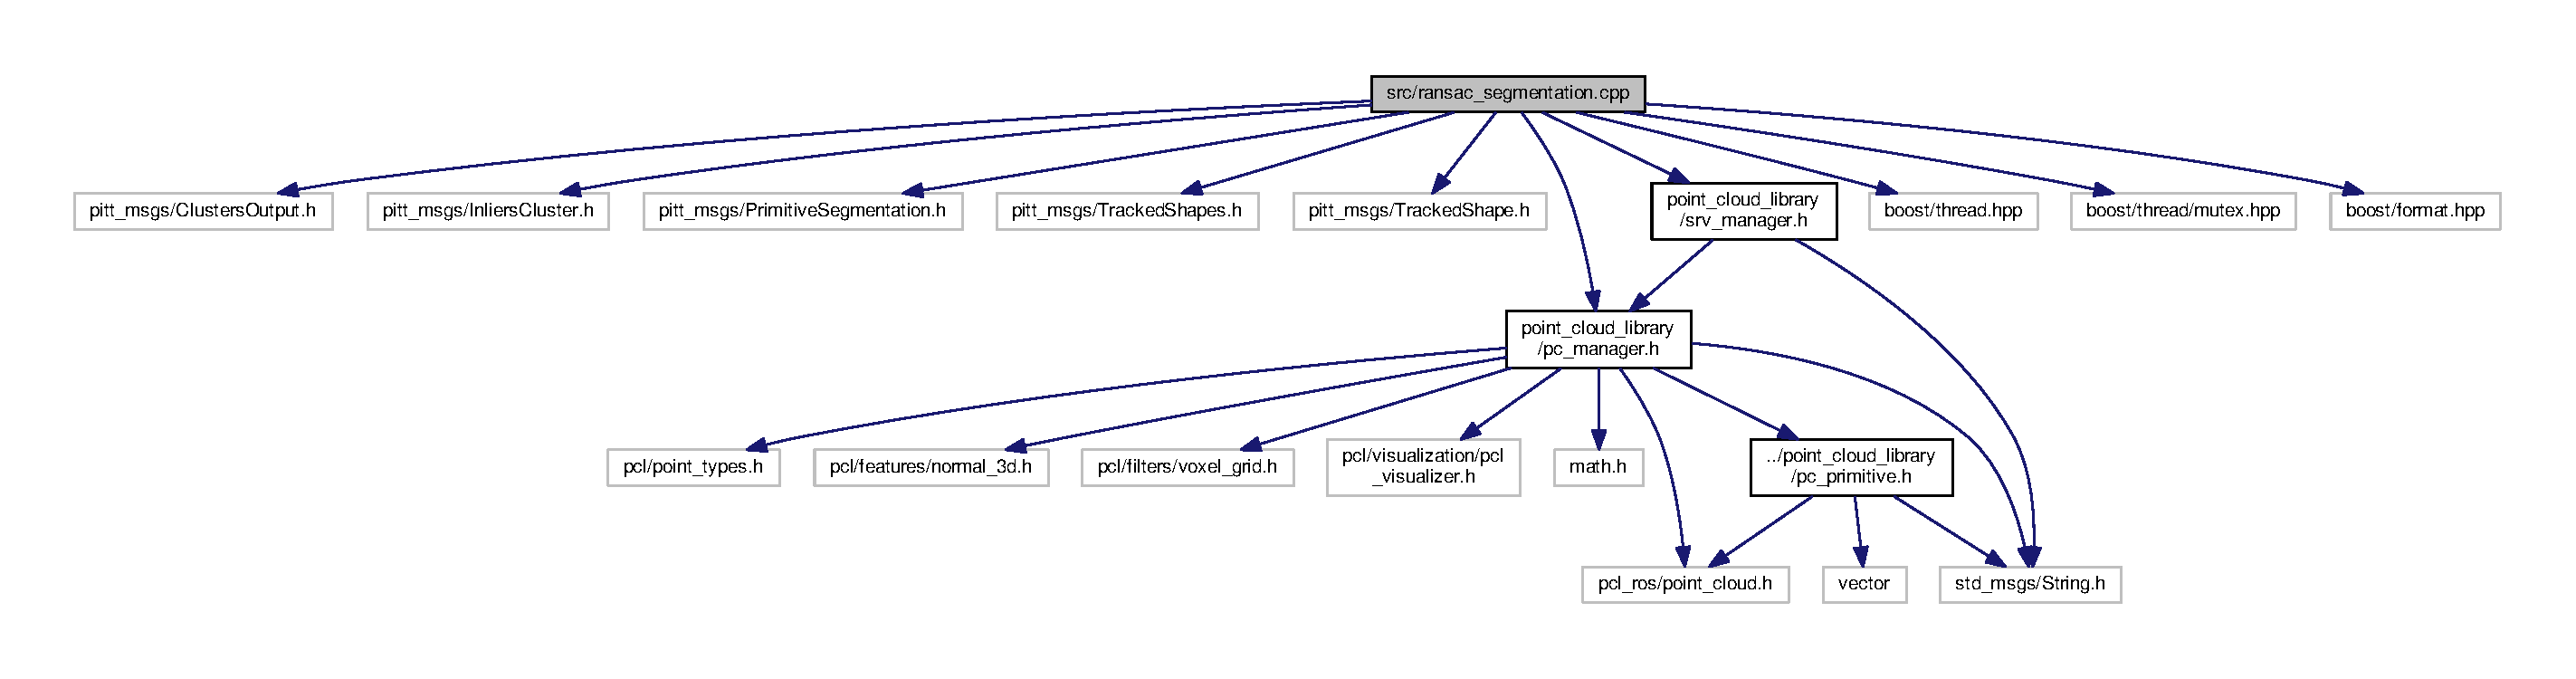
\includegraphics[width=350pt]{ransac__segmentation_8cpp__incl}
\end{center}
\end{figure}
\subsection*{Typedefs}
\begin{DoxyCompactItemize}
\item 
typedef vector$<$ Inliers\-Cluster $>$ \hyperlink{ransac__segmentation_8cpp_a48bae868bfe27bed6e11eeb5c77b062a}{Inliers\-Clusters}
\item 
typedef boost\-::shared\-\_\-ptr\\*
$<$ \hyperlink{ransac__segmentation_8cpp_a48bae868bfe27bed6e11eeb5c77b062a}{Inliers\-Clusters} $>$ \hyperlink{ransac__segmentation_8cpp_af1cdfa162edb0b94902557379b5cf42d}{Inliers\-Clusters\-Ptr}
\item 
typedef boost\-::shared\-\_\-ptr\\*
$<$ Primitive\-Segmentation $>$ \hyperlink{ransac__segmentation_8cpp_aadce7a04d47ab4d0099588791d834045}{Primitive\-Segmentation\-Ptr}
\end{DoxyCompactItemize}
\subsection*{Functions}
\begin{DoxyCompactItemize}
\item 
void \hyperlink{ransac__segmentation_8cpp_aca73ab26cae45b4b998a3cca9e4f75bc}{vis\-Spin} ()
\item 
bool \hyperlink{ransac__segmentation_8cpp_a1c975f4a118598c3ab7eff48fa749476}{call\-Ransac\-Sphere\-Segmentation} (\hyperlink{pc__primitive_8h_aa14a240c8d999c4f56133c0f70e88783}{P\-C\-L\-Cloud\-Ptr} cloud, \hyperlink{pc__primitive_8h_a1bc38ce8b0c26e5f2d28fae9f3e3ea97}{P\-C\-L\-Normal\-Ptr} norm, \hyperlink{ransac__segmentation_8cpp_aadce7a04d47ab4d0099588791d834045}{Primitive\-Segmentation\-Ptr} \&out)
\item 
void \hyperlink{ransac__segmentation_8cpp_a575e2f0efaeee850e608ac4481557314}{print\-Sphere\-Info} (\hyperlink{ransac__segmentation_8cpp_aadce7a04d47ab4d0099588791d834045}{Primitive\-Segmentation\-Ptr} info, int idx)
\item 
bool \hyperlink{ransac__segmentation_8cpp_a850aede9ccf4da9338681e9ea25b50c6}{call\-Ransac\-Cylinder\-Segmentation} (\hyperlink{pc__primitive_8h_aa14a240c8d999c4f56133c0f70e88783}{P\-C\-L\-Cloud\-Ptr} cloud, \hyperlink{pc__primitive_8h_a1bc38ce8b0c26e5f2d28fae9f3e3ea97}{P\-C\-L\-Normal\-Ptr} norm, \hyperlink{ransac__segmentation_8cpp_aadce7a04d47ab4d0099588791d834045}{Primitive\-Segmentation\-Ptr} \&out)
\item 
void \hyperlink{ransac__segmentation_8cpp_a45c30fa927c0717d8346839fd1c68bde}{print\-Cylinder\-Info} (\hyperlink{ransac__segmentation_8cpp_aadce7a04d47ab4d0099588791d834045}{Primitive\-Segmentation\-Ptr} info, int idx)
\item 
bool \hyperlink{ransac__segmentation_8cpp_aec52b04d4f14e655979ec0316bab27be}{call\-Ransac\-Cone\-Segmentation} (\hyperlink{pc__primitive_8h_aa14a240c8d999c4f56133c0f70e88783}{P\-C\-L\-Cloud\-Ptr} cloud, \hyperlink{pc__primitive_8h_a1bc38ce8b0c26e5f2d28fae9f3e3ea97}{P\-C\-L\-Normal\-Ptr} norm, \hyperlink{ransac__segmentation_8cpp_aadce7a04d47ab4d0099588791d834045}{Primitive\-Segmentation\-Ptr} \&out)
\item 
void \hyperlink{ransac__segmentation_8cpp_a7e84119f095d7369dc280ca585dcd9fb}{print\-Cone\-Info} (\hyperlink{ransac__segmentation_8cpp_aadce7a04d47ab4d0099588791d834045}{Primitive\-Segmentation\-Ptr} info, int idx)
\item 
bool \hyperlink{ransac__segmentation_8cpp_afcfa79d6f194e0e582affcad49fec033}{call\-Ransac\-Plane\-Segmentation} (\hyperlink{pc__primitive_8h_aa14a240c8d999c4f56133c0f70e88783}{P\-C\-L\-Cloud\-Ptr} cloud, \hyperlink{pc__primitive_8h_a1bc38ce8b0c26e5f2d28fae9f3e3ea97}{P\-C\-L\-Normal\-Ptr} norm, \hyperlink{ransac__segmentation_8cpp_aadce7a04d47ab4d0099588791d834045}{Primitive\-Segmentation\-Ptr} \&out)
\item 
void \hyperlink{ransac__segmentation_8cpp_a20792e9769230baa8e2258731a5143de}{print\-Plane\-Info} (\hyperlink{ransac__segmentation_8cpp_aadce7a04d47ab4d0099588791d834045}{Primitive\-Segmentation\-Ptr} info, int idx)
\item 
string \hyperlink{ransac__segmentation_8cpp_a9fce32945b78e03d2b0abde7198fe623}{return\-Primitive\-Name\-From\-Tag} (int primitive\-Tag)
\item 
void \hyperlink{ransac__segmentation_8cpp_a87bb87e16486622aae18704555f5af81}{clusters\-Acquisition} (const Clusters\-Output\-Const\-Ptr \&cluster\-Obj)
\item 
int \hyperlink{ransac__segmentation_8cpp_a3c04138a5bfe5d72780bb7e82a18e627}{main} (int argc, char $\ast$$\ast$argv)
\end{DoxyCompactItemize}
\subsection*{Variables}
\begin{DoxyCompactItemize}
\item 
ros\-::\-Node\-Handle $\ast$ \hyperlink{ransac__segmentation_8cpp_afe3fec681d3658d114dfa8cfff163e82}{nh\-\_\-ptr} = N\-U\-L\-L
\item 
boost\-::shared\-\_\-ptr\\*
$<$ \hyperlink{pc__manager_8h_a38c805dbc7ad6f06109b85c8e540817a}{visualization\-::\-P\-C\-L\-Visualizer} $>$ \hyperlink{ransac__segmentation_8cpp_a6c2d87234fca8dcca11f888098558986}{vis}
\item 
boost\-::thread \hyperlink{ransac__segmentation_8cpp_ab83e6219895a4d26706c0d858f8ec288}{vis\-\_\-thread}
\item 
boost\-::mutex \hyperlink{ransac__segmentation_8cpp_a0dc8882293908d9c8cc15f76a2a49588}{vis\-\_\-mutex}
\item 
Publisher \hyperlink{ransac__segmentation_8cpp_a13f806db112b4cc50fbdc2bc57078c28}{pub}
\item 
static const int \hyperlink{ransac__segmentation_8cpp_adb867ab4ac1ea252546319b4c5d8fe27}{D\-E\-F\-A\-U\-L\-T\-\_\-\-S\-P\-H\-E\-R\-E\-\_\-\-M\-I\-N\-\_\-\-I\-N\-L\-I\-E\-R\-S} = 40
\item 
static const int \hyperlink{ransac__segmentation_8cpp_a5f761c5c4b185a395c4c9808feb95d95}{D\-E\-F\-A\-U\-L\-T\-\_\-\-C\-Y\-L\-I\-N\-D\-E\-R\-\_\-\-M\-I\-N\-\_\-\-I\-N\-L\-I\-E\-R\-S} = 40
\item 
static const int \hyperlink{ransac__segmentation_8cpp_a2f01afe51b5f0fe549a9d45901d67436}{D\-E\-F\-A\-U\-L\-T\-\_\-\-C\-O\-N\-E\-\_\-\-M\-I\-N\-\_\-\-I\-N\-L\-I\-E\-R\-S} = 40
\item 
static const int \hyperlink{ransac__segmentation_8cpp_acaaec88a430023775eff009968b1708f}{D\-E\-F\-A\-U\-L\-T\-\_\-\-P\-L\-A\-N\-E\-\_\-\-M\-I\-N\-\_\-\-I\-N\-L\-I\-E\-R\-S} = 40
\item 
static const float \hyperlink{ransac__segmentation_8cpp_a85bdb530100d3d064078d3d7c89df94d}{D\-E\-F\-A\-U\-L\-T\-\_\-\-C\-O\-N\-E\-\_\-\-O\-V\-E\-R\-\_\-\-C\-Y\-L\-I\-N\-D\-E\-R\-\_\-\-P\-R\-I\-O\-R\-I\-T\-Y} = 0.\-9f
\item 
static const bool \hyperlink{ransac__segmentation_8cpp_a1fdd3984211ccefc7674b8b1fa1f49df}{D\-E\-F\-A\-U\-L\-T\-\_\-\-S\-H\-O\-W\-\_\-\-P\-R\-I\-M\-I\-T\-I\-V\-E} = false
\item 
static bool \hyperlink{ransac__segmentation_8cpp_a18bf0a1b07fdaa1e7b9ab561a9bdabaf}{S\-H\-O\-W\-\_\-\-P\-R\-I\-M\-I\-T\-I\-V\-E}
\item 
static const int \hyperlink{ransac__segmentation_8cpp_ae40d37f99c64adbd93effecc8b752907}{T\-X\-T\-\_\-\-U\-N\-K\-N\-O\-W\-N\-\_\-\-S\-H\-A\-P\-E\-\_\-\-T\-A\-G} = 0
\item 
static const int \hyperlink{ransac__segmentation_8cpp_a47ddbf099646e58710140cf3679f72f2}{T\-X\-T\-\_\-\-P\-L\-A\-N\-E\-\_\-\-S\-H\-A\-P\-E\-\_\-\-T\-A\-G} = 1
\item 
static const int \hyperlink{ransac__segmentation_8cpp_a3f9053cbbd25a97e8c388045da67a408}{T\-X\-T\-\_\-\-S\-P\-H\-E\-R\-E\-\_\-\-S\-H\-A\-P\-E\-\_\-\-T\-A\-G} = 2
\item 
static const int \hyperlink{ransac__segmentation_8cpp_af67dfc98bd4ee810ddc6a839a6aae211}{T\-X\-T\-\_\-\-C\-O\-N\-E\-\_\-\-S\-H\-A\-P\-E\-\_\-\-T\-A\-G} = 3
\item 
static const int \hyperlink{ransac__segmentation_8cpp_a68959196886065740b4f24500e726e6f}{T\-X\-T\-\_\-\-C\-Y\-L\-I\-N\-D\-E\-R\-\_\-\-S\-H\-A\-P\-E\-\_\-\-T\-A\-G} = 4
\item 
int \hyperlink{ransac__segmentation_8cpp_ab50798a62f439e3d4f3e5a62c5c5c54c}{sphere\-Min\-Inliers}
\item 
int \hyperlink{ransac__segmentation_8cpp_a3dffb746534aa3e73b59a17089d93612}{cylinder\-Min\-Inliers}
\item 
int \hyperlink{ransac__segmentation_8cpp_aff83bb933480fbc147b205bf335182d6}{cone\-Min\-Inliers}
\item 
int \hyperlink{ransac__segmentation_8cpp_acb1b4dd3aad99e7793bc2301c7e15742}{plane\-Min\-Inliers}
\item 
int \hyperlink{ransac__segmentation_8cpp_a10547ce154fba3eee4db9557b0399fba}{cone\-Over\-Cylinder\-Priority}
\item 
string \hyperlink{ransac__segmentation_8cpp_a89794ef3f62d4bfa2dba13649e279e58}{centroid\-File\-Log}
\end{DoxyCompactItemize}


\subsection{Typedef Documentation}
\hypertarget{ransac__segmentation_8cpp_a48bae868bfe27bed6e11eeb5c77b062a}{\index{ransac\-\_\-segmentation.\-cpp@{ransac\-\_\-segmentation.\-cpp}!Inliers\-Clusters@{Inliers\-Clusters}}
\index{Inliers\-Clusters@{Inliers\-Clusters}!ransac_segmentation.cpp@{ransac\-\_\-segmentation.\-cpp}}
\subsubsection[{Inliers\-Clusters}]{\setlength{\rightskip}{0pt plus 5cm}typedef vector$<$ Inliers\-Cluster$>$ {\bf Inliers\-Clusters}}}\label{ransac__segmentation_8cpp_a48bae868bfe27bed6e11eeb5c77b062a}


Definition at line 20 of file ransac\-\_\-segmentation.\-cpp.

\hypertarget{ransac__segmentation_8cpp_af1cdfa162edb0b94902557379b5cf42d}{\index{ransac\-\_\-segmentation.\-cpp@{ransac\-\_\-segmentation.\-cpp}!Inliers\-Clusters\-Ptr@{Inliers\-Clusters\-Ptr}}
\index{Inliers\-Clusters\-Ptr@{Inliers\-Clusters\-Ptr}!ransac_segmentation.cpp@{ransac\-\_\-segmentation.\-cpp}}
\subsubsection[{Inliers\-Clusters\-Ptr}]{\setlength{\rightskip}{0pt plus 5cm}typedef boost\-::shared\-\_\-ptr$<$ {\bf Inliers\-Clusters}$>$ {\bf Inliers\-Clusters\-Ptr}}}\label{ransac__segmentation_8cpp_af1cdfa162edb0b94902557379b5cf42d}


Definition at line 21 of file ransac\-\_\-segmentation.\-cpp.

\hypertarget{ransac__segmentation_8cpp_aadce7a04d47ab4d0099588791d834045}{\index{ransac\-\_\-segmentation.\-cpp@{ransac\-\_\-segmentation.\-cpp}!Primitive\-Segmentation\-Ptr@{Primitive\-Segmentation\-Ptr}}
\index{Primitive\-Segmentation\-Ptr@{Primitive\-Segmentation\-Ptr}!ransac_segmentation.cpp@{ransac\-\_\-segmentation.\-cpp}}
\subsubsection[{Primitive\-Segmentation\-Ptr}]{\setlength{\rightskip}{0pt plus 5cm}typedef boost\-::shared\-\_\-ptr$<$ Primitive\-Segmentation$>$ {\bf Primitive\-Segmentation\-Ptr}}}\label{ransac__segmentation_8cpp_aadce7a04d47ab4d0099588791d834045}


Definition at line 22 of file ransac\-\_\-segmentation.\-cpp.



\subsection{Function Documentation}
\hypertarget{ransac__segmentation_8cpp_aec52b04d4f14e655979ec0316bab27be}{\index{ransac\-\_\-segmentation.\-cpp@{ransac\-\_\-segmentation.\-cpp}!call\-Ransac\-Cone\-Segmentation@{call\-Ransac\-Cone\-Segmentation}}
\index{call\-Ransac\-Cone\-Segmentation@{call\-Ransac\-Cone\-Segmentation}!ransac_segmentation.cpp@{ransac\-\_\-segmentation.\-cpp}}
\subsubsection[{call\-Ransac\-Cone\-Segmentation}]{\setlength{\rightskip}{0pt plus 5cm}bool call\-Ransac\-Cone\-Segmentation (
\begin{DoxyParamCaption}
\item[{{\bf P\-C\-L\-Cloud\-Ptr}}]{cloud, }
\item[{{\bf P\-C\-L\-Normal\-Ptr}}]{norm, }
\item[{{\bf Primitive\-Segmentation\-Ptr} \&}]{out}
\end{DoxyParamCaption}
)}}\label{ransac__segmentation_8cpp_aec52b04d4f14e655979ec0316bab27be}


Definition at line 135 of file ransac\-\_\-segmentation.\-cpp.



References cone\-Min\-Inliers, D\-E\-F\-A\-U\-L\-T\-\_\-\-C\-O\-N\-E\-\_\-\-M\-I\-N\-\_\-\-I\-N\-L\-I\-E\-R\-S, nh\-\_\-ptr, srvm\-::\-P\-A\-R\-A\-M\-\_\-\-N\-A\-M\-E\-\_\-\-C\-O\-N\-E\-\_\-\-M\-I\-N\-\_\-\-I\-N\-L\-I\-E\-R\-S, and srvm\-::\-S\-R\-V\-\_\-\-N\-A\-M\-E\-\_\-\-R\-A\-N\-S\-A\-C\-\_\-\-C\-O\-N\-E\-\_\-\-F\-I\-L\-T\-E\-R.



Referenced by clusters\-Acquisition().

\hypertarget{ransac__segmentation_8cpp_a850aede9ccf4da9338681e9ea25b50c6}{\index{ransac\-\_\-segmentation.\-cpp@{ransac\-\_\-segmentation.\-cpp}!call\-Ransac\-Cylinder\-Segmentation@{call\-Ransac\-Cylinder\-Segmentation}}
\index{call\-Ransac\-Cylinder\-Segmentation@{call\-Ransac\-Cylinder\-Segmentation}!ransac_segmentation.cpp@{ransac\-\_\-segmentation.\-cpp}}
\subsubsection[{call\-Ransac\-Cylinder\-Segmentation}]{\setlength{\rightskip}{0pt plus 5cm}bool call\-Ransac\-Cylinder\-Segmentation (
\begin{DoxyParamCaption}
\item[{{\bf P\-C\-L\-Cloud\-Ptr}}]{cloud, }
\item[{{\bf P\-C\-L\-Normal\-Ptr}}]{norm, }
\item[{{\bf Primitive\-Segmentation\-Ptr} \&}]{out}
\end{DoxyParamCaption}
)}}\label{ransac__segmentation_8cpp_a850aede9ccf4da9338681e9ea25b50c6}


Definition at line 96 of file ransac\-\_\-segmentation.\-cpp.



References cylinder\-Min\-Inliers, D\-E\-F\-A\-U\-L\-T\-\_\-\-C\-Y\-L\-I\-N\-D\-E\-R\-\_\-\-M\-I\-N\-\_\-\-I\-N\-L\-I\-E\-R\-S, nh\-\_\-ptr, srvm\-::\-P\-A\-R\-A\-M\-\_\-\-N\-A\-M\-E\-\_\-\-C\-Y\-L\-I\-N\-D\-E\-R\-\_\-\-M\-I\-N\-\_\-\-I\-N\-L\-I\-E\-R\-S, and srvm\-::\-S\-R\-V\-\_\-\-N\-A\-M\-E\-\_\-\-R\-A\-N\-S\-A\-C\-\_\-\-C\-Y\-L\-I\-N\-D\-E\-R\-\_\-\-F\-I\-L\-T\-E\-R.



Referenced by clusters\-Acquisition().

\hypertarget{ransac__segmentation_8cpp_afcfa79d6f194e0e582affcad49fec033}{\index{ransac\-\_\-segmentation.\-cpp@{ransac\-\_\-segmentation.\-cpp}!call\-Ransac\-Plane\-Segmentation@{call\-Ransac\-Plane\-Segmentation}}
\index{call\-Ransac\-Plane\-Segmentation@{call\-Ransac\-Plane\-Segmentation}!ransac_segmentation.cpp@{ransac\-\_\-segmentation.\-cpp}}
\subsubsection[{call\-Ransac\-Plane\-Segmentation}]{\setlength{\rightskip}{0pt plus 5cm}bool call\-Ransac\-Plane\-Segmentation (
\begin{DoxyParamCaption}
\item[{{\bf P\-C\-L\-Cloud\-Ptr}}]{cloud, }
\item[{{\bf P\-C\-L\-Normal\-Ptr}}]{norm, }
\item[{{\bf Primitive\-Segmentation\-Ptr} \&}]{out}
\end{DoxyParamCaption}
)}}\label{ransac__segmentation_8cpp_afcfa79d6f194e0e582affcad49fec033}


Definition at line 175 of file ransac\-\_\-segmentation.\-cpp.



References D\-E\-F\-A\-U\-L\-T\-\_\-\-P\-L\-A\-N\-E\-\_\-\-M\-I\-N\-\_\-\-I\-N\-L\-I\-E\-R\-S, nh\-\_\-ptr, srvm\-::\-P\-A\-R\-A\-M\-\_\-\-N\-A\-M\-E\-\_\-\-P\-L\-A\-N\-E\-\_\-\-M\-I\-N\-\_\-\-I\-N\-L\-I\-E\-R\-S, plane\-Min\-Inliers, and srvm\-::\-S\-R\-V\-\_\-\-N\-A\-M\-E\-\_\-\-R\-A\-N\-S\-A\-C\-\_\-\-P\-L\-A\-N\-E\-\_\-\-F\-I\-L\-T\-E\-R.



Referenced by clusters\-Acquisition().

\hypertarget{ransac__segmentation_8cpp_a1c975f4a118598c3ab7eff48fa749476}{\index{ransac\-\_\-segmentation.\-cpp@{ransac\-\_\-segmentation.\-cpp}!call\-Ransac\-Sphere\-Segmentation@{call\-Ransac\-Sphere\-Segmentation}}
\index{call\-Ransac\-Sphere\-Segmentation@{call\-Ransac\-Sphere\-Segmentation}!ransac_segmentation.cpp@{ransac\-\_\-segmentation.\-cpp}}
\subsubsection[{call\-Ransac\-Sphere\-Segmentation}]{\setlength{\rightskip}{0pt plus 5cm}bool call\-Ransac\-Sphere\-Segmentation (
\begin{DoxyParamCaption}
\item[{{\bf P\-C\-L\-Cloud\-Ptr}}]{cloud, }
\item[{{\bf P\-C\-L\-Normal\-Ptr}}]{norm, }
\item[{{\bf Primitive\-Segmentation\-Ptr} \&}]{out}
\end{DoxyParamCaption}
)}}\label{ransac__segmentation_8cpp_a1c975f4a118598c3ab7eff48fa749476}


Definition at line 58 of file ransac\-\_\-segmentation.\-cpp.



References D\-E\-F\-A\-U\-L\-T\-\_\-\-S\-P\-H\-E\-R\-E\-\_\-\-M\-I\-N\-\_\-\-I\-N\-L\-I\-E\-R\-S, nh\-\_\-ptr, srvm\-::\-P\-A\-R\-A\-M\-\_\-\-N\-A\-M\-E\-\_\-\-S\-P\-H\-E\-R\-E\-\_\-\-M\-I\-N\-\_\-\-I\-N\-L\-I\-E\-R\-S, sphere\-Min\-Inliers, and srvm\-::\-S\-R\-V\-\_\-\-N\-A\-M\-E\-\_\-\-R\-A\-N\-S\-A\-C\-\_\-\-S\-P\-H\-E\-R\-E\-\_\-\-F\-I\-L\-T\-E\-R.



Referenced by clusters\-Acquisition().

\hypertarget{ransac__segmentation_8cpp_a87bb87e16486622aae18704555f5af81}{\index{ransac\-\_\-segmentation.\-cpp@{ransac\-\_\-segmentation.\-cpp}!clusters\-Acquisition@{clusters\-Acquisition}}
\index{clusters\-Acquisition@{clusters\-Acquisition}!ransac_segmentation.cpp@{ransac\-\_\-segmentation.\-cpp}}
\subsubsection[{clusters\-Acquisition}]{\setlength{\rightskip}{0pt plus 5cm}void clusters\-Acquisition (
\begin{DoxyParamCaption}
\item[{const Clusters\-Output\-Const\-Ptr \&}]{cluster\-Obj}
\end{DoxyParamCaption}
)}}\label{ransac__segmentation_8cpp_a87bb87e16486622aae18704555f5af81}


Definition at line 223 of file ransac\-\_\-segmentation.\-cpp.



References call\-Ransac\-Cone\-Segmentation(), call\-Ransac\-Cylinder\-Segmentation(), call\-Ransac\-Plane\-Segmentation(), call\-Ransac\-Sphere\-Segmentation(), cone\-Min\-Inliers, cylinder\-Min\-Inliers, D\-E\-F\-A\-U\-L\-T\-\_\-\-C\-O\-N\-E\-\_\-\-O\-V\-E\-R\-\_\-\-C\-Y\-L\-I\-N\-D\-E\-R\-\_\-\-P\-R\-I\-O\-R\-I\-T\-Y, plane\-Min\-Inliers, pub, return\-Primitive\-Name\-From\-Tag(), S\-H\-O\-W\-\_\-\-P\-R\-I\-M\-I\-T\-I\-V\-E, sphere\-Min\-Inliers, T\-X\-T\-\_\-\-C\-O\-N\-E\-\_\-\-S\-H\-A\-P\-E\-\_\-\-T\-A\-G, T\-X\-T\-\_\-\-C\-Y\-L\-I\-N\-D\-E\-R\-\_\-\-S\-H\-A\-P\-E\-\_\-\-T\-A\-G, T\-X\-T\-\_\-\-P\-L\-A\-N\-E\-\_\-\-S\-H\-A\-P\-E\-\_\-\-T\-A\-G, T\-X\-T\-\_\-\-S\-P\-H\-E\-R\-E\-\_\-\-S\-H\-A\-P\-E\-\_\-\-T\-A\-G, T\-X\-T\-\_\-\-U\-N\-K\-N\-O\-W\-N\-\_\-\-S\-H\-A\-P\-E\-\_\-\-T\-A\-G, vis, and vis\-\_\-mutex.



Referenced by main().



Here is the call graph for this function\-:
\nopagebreak
\begin{figure}[H]
\begin{center}
\leavevmode
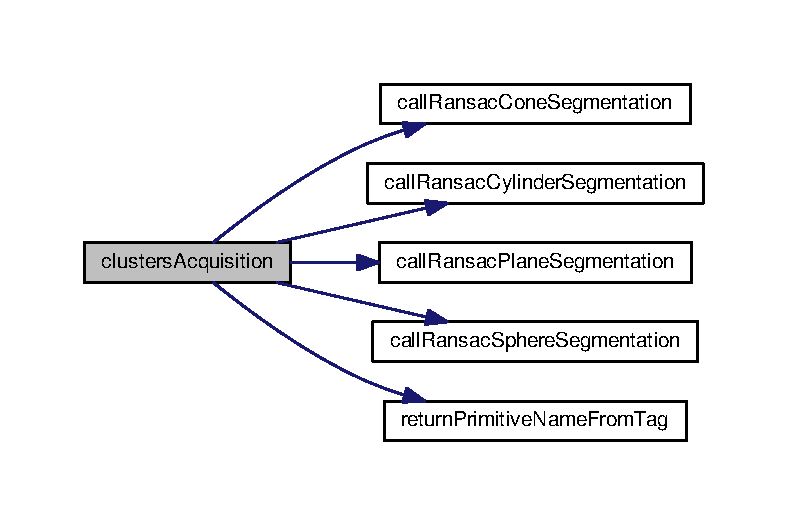
\includegraphics[width=350pt]{ransac__segmentation_8cpp_a87bb87e16486622aae18704555f5af81_cgraph}
\end{center}
\end{figure}


\hypertarget{ransac__segmentation_8cpp_a3c04138a5bfe5d72780bb7e82a18e627}{\index{ransac\-\_\-segmentation.\-cpp@{ransac\-\_\-segmentation.\-cpp}!main@{main}}
\index{main@{main}!ransac_segmentation.cpp@{ransac\-\_\-segmentation.\-cpp}}
\subsubsection[{main}]{\setlength{\rightskip}{0pt plus 5cm}int main (
\begin{DoxyParamCaption}
\item[{int}]{argc, }
\item[{char $\ast$$\ast$}]{argv}
\end{DoxyParamCaption}
)}}\label{ransac__segmentation_8cpp_a3c04138a5bfe5d72780bb7e82a18e627}


Definition at line 347 of file ransac\-\_\-segmentation.\-cpp.



References centroid\-File\-Log, clusters\-Acquisition(), D\-E\-F\-A\-U\-L\-T\-\_\-\-C\-O\-N\-E\-\_\-\-M\-I\-N\-\_\-\-I\-N\-L\-I\-E\-R\-S, D\-E\-F\-A\-U\-L\-T\-\_\-\-C\-O\-N\-E\-\_\-\-O\-V\-E\-R\-\_\-\-C\-Y\-L\-I\-N\-D\-E\-R\-\_\-\-P\-R\-I\-O\-R\-I\-T\-Y, D\-E\-F\-A\-U\-L\-T\-\_\-\-C\-Y\-L\-I\-N\-D\-E\-R\-\_\-\-M\-I\-N\-\_\-\-I\-N\-L\-I\-E\-R\-S, D\-E\-F\-A\-U\-L\-T\-\_\-\-P\-L\-A\-N\-E\-\_\-\-M\-I\-N\-\_\-\-I\-N\-L\-I\-E\-R\-S, D\-E\-F\-A\-U\-L\-T\-\_\-\-S\-H\-O\-W\-\_\-\-P\-R\-I\-M\-I\-T\-I\-V\-E, D\-E\-F\-A\-U\-L\-T\-\_\-\-S\-P\-H\-E\-R\-E\-\_\-\-M\-I\-N\-\_\-\-I\-N\-L\-I\-E\-R\-S, srvm\-::get\-Bool\-Ptr\-Parameter(), nh\-\_\-ptr, pub, S\-H\-O\-W\-\_\-\-P\-R\-I\-M\-I\-T\-I\-V\-E, vis, vis\-\_\-thread, and vis\-Spin().



Here is the call graph for this function\-:
\nopagebreak
\begin{figure}[H]
\begin{center}
\leavevmode
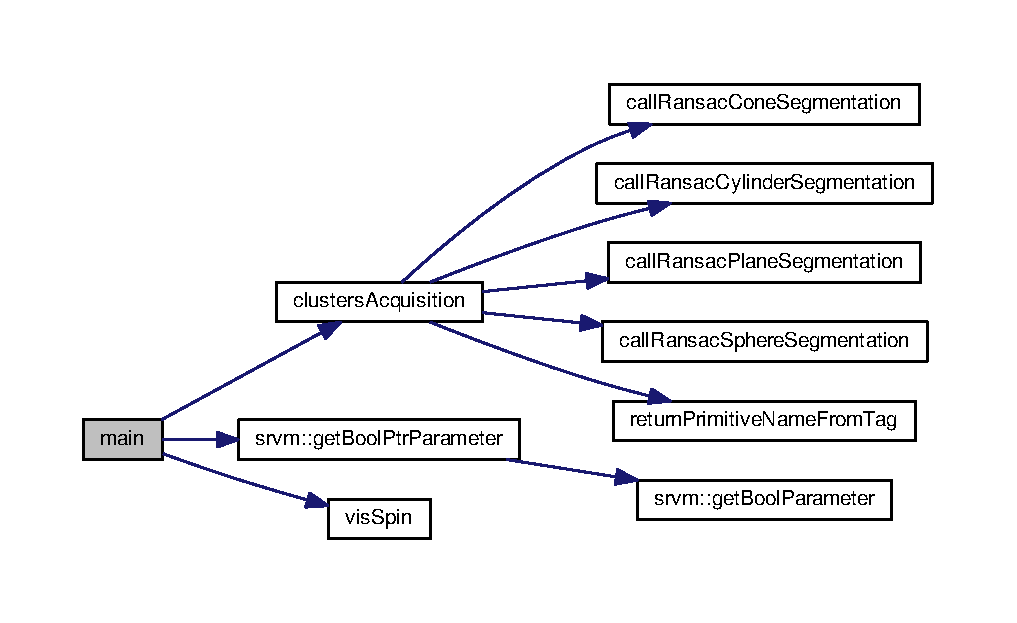
\includegraphics[width=350pt]{ransac__segmentation_8cpp_a3c04138a5bfe5d72780bb7e82a18e627_cgraph}
\end{center}
\end{figure}


\hypertarget{ransac__segmentation_8cpp_a7e84119f095d7369dc280ca585dcd9fb}{\index{ransac\-\_\-segmentation.\-cpp@{ransac\-\_\-segmentation.\-cpp}!print\-Cone\-Info@{print\-Cone\-Info}}
\index{print\-Cone\-Info@{print\-Cone\-Info}!ransac_segmentation.cpp@{ransac\-\_\-segmentation.\-cpp}}
\subsubsection[{print\-Cone\-Info}]{\setlength{\rightskip}{0pt plus 5cm}void print\-Cone\-Info (
\begin{DoxyParamCaption}
\item[{{\bf Primitive\-Segmentation\-Ptr}}]{info, }
\item[{int}]{idx}
\end{DoxyParamCaption}
)}}\label{ransac__segmentation_8cpp_a7e84119f095d7369dc280ca585dcd9fb}


Definition at line 161 of file ransac\-\_\-segmentation.\-cpp.

\hypertarget{ransac__segmentation_8cpp_a45c30fa927c0717d8346839fd1c68bde}{\index{ransac\-\_\-segmentation.\-cpp@{ransac\-\_\-segmentation.\-cpp}!print\-Cylinder\-Info@{print\-Cylinder\-Info}}
\index{print\-Cylinder\-Info@{print\-Cylinder\-Info}!ransac_segmentation.cpp@{ransac\-\_\-segmentation.\-cpp}}
\subsubsection[{print\-Cylinder\-Info}]{\setlength{\rightskip}{0pt plus 5cm}void print\-Cylinder\-Info (
\begin{DoxyParamCaption}
\item[{{\bf Primitive\-Segmentation\-Ptr}}]{info, }
\item[{int}]{idx}
\end{DoxyParamCaption}
)}}\label{ransac__segmentation_8cpp_a45c30fa927c0717d8346839fd1c68bde}


Definition at line 122 of file ransac\-\_\-segmentation.\-cpp.

\hypertarget{ransac__segmentation_8cpp_a20792e9769230baa8e2258731a5143de}{\index{ransac\-\_\-segmentation.\-cpp@{ransac\-\_\-segmentation.\-cpp}!print\-Plane\-Info@{print\-Plane\-Info}}
\index{print\-Plane\-Info@{print\-Plane\-Info}!ransac_segmentation.cpp@{ransac\-\_\-segmentation.\-cpp}}
\subsubsection[{print\-Plane\-Info}]{\setlength{\rightskip}{0pt plus 5cm}void print\-Plane\-Info (
\begin{DoxyParamCaption}
\item[{{\bf Primitive\-Segmentation\-Ptr}}]{info, }
\item[{int}]{idx}
\end{DoxyParamCaption}
)}}\label{ransac__segmentation_8cpp_a20792e9769230baa8e2258731a5143de}


Definition at line 201 of file ransac\-\_\-segmentation.\-cpp.

\hypertarget{ransac__segmentation_8cpp_a575e2f0efaeee850e608ac4481557314}{\index{ransac\-\_\-segmentation.\-cpp@{ransac\-\_\-segmentation.\-cpp}!print\-Sphere\-Info@{print\-Sphere\-Info}}
\index{print\-Sphere\-Info@{print\-Sphere\-Info}!ransac_segmentation.cpp@{ransac\-\_\-segmentation.\-cpp}}
\subsubsection[{print\-Sphere\-Info}]{\setlength{\rightskip}{0pt plus 5cm}void print\-Sphere\-Info (
\begin{DoxyParamCaption}
\item[{{\bf Primitive\-Segmentation\-Ptr}}]{info, }
\item[{int}]{idx}
\end{DoxyParamCaption}
)}}\label{ransac__segmentation_8cpp_a575e2f0efaeee850e608ac4481557314}


Definition at line 86 of file ransac\-\_\-segmentation.\-cpp.

\hypertarget{ransac__segmentation_8cpp_a9fce32945b78e03d2b0abde7198fe623}{\index{ransac\-\_\-segmentation.\-cpp@{ransac\-\_\-segmentation.\-cpp}!return\-Primitive\-Name\-From\-Tag@{return\-Primitive\-Name\-From\-Tag}}
\index{return\-Primitive\-Name\-From\-Tag@{return\-Primitive\-Name\-From\-Tag}!ransac_segmentation.cpp@{ransac\-\_\-segmentation.\-cpp}}
\subsubsection[{return\-Primitive\-Name\-From\-Tag}]{\setlength{\rightskip}{0pt plus 5cm}string return\-Primitive\-Name\-From\-Tag (
\begin{DoxyParamCaption}
\item[{int}]{primitive\-Tag}
\end{DoxyParamCaption}
)}}\label{ransac__segmentation_8cpp_a9fce32945b78e03d2b0abde7198fe623}


Definition at line 210 of file ransac\-\_\-segmentation.\-cpp.



References T\-X\-T\-\_\-\-C\-O\-N\-E\-\_\-\-S\-H\-A\-P\-E\-\_\-\-T\-A\-G, T\-X\-T\-\_\-\-C\-Y\-L\-I\-N\-D\-E\-R\-\_\-\-S\-H\-A\-P\-E\-\_\-\-T\-A\-G, T\-X\-T\-\_\-\-P\-L\-A\-N\-E\-\_\-\-S\-H\-A\-P\-E\-\_\-\-T\-A\-G, T\-X\-T\-\_\-\-S\-P\-H\-E\-R\-E\-\_\-\-S\-H\-A\-P\-E\-\_\-\-T\-A\-G, and T\-X\-T\-\_\-\-U\-N\-K\-N\-O\-W\-N\-\_\-\-S\-H\-A\-P\-E\-\_\-\-T\-A\-G.



Referenced by clusters\-Acquisition().

\hypertarget{ransac__segmentation_8cpp_aca73ab26cae45b4b998a3cca9e4f75bc}{\index{ransac\-\_\-segmentation.\-cpp@{ransac\-\_\-segmentation.\-cpp}!vis\-Spin@{vis\-Spin}}
\index{vis\-Spin@{vis\-Spin}!ransac_segmentation.cpp@{ransac\-\_\-segmentation.\-cpp}}
\subsubsection[{vis\-Spin}]{\setlength{\rightskip}{0pt plus 5cm}void vis\-Spin (
\begin{DoxyParamCaption}
{}
\end{DoxyParamCaption}
)}}\label{ransac__segmentation_8cpp_aca73ab26cae45b4b998a3cca9e4f75bc}


Definition at line 50 of file ransac\-\_\-segmentation.\-cpp.



References vis, and vis\-\_\-mutex.



Referenced by main().



\subsection{Variable Documentation}
\hypertarget{ransac__segmentation_8cpp_a89794ef3f62d4bfa2dba13649e279e58}{\index{ransac\-\_\-segmentation.\-cpp@{ransac\-\_\-segmentation.\-cpp}!centroid\-File\-Log@{centroid\-File\-Log}}
\index{centroid\-File\-Log@{centroid\-File\-Log}!ransac_segmentation.cpp@{ransac\-\_\-segmentation.\-cpp}}
\subsubsection[{centroid\-File\-Log}]{\setlength{\rightskip}{0pt plus 5cm}string centroid\-File\-Log}}\label{ransac__segmentation_8cpp_a89794ef3f62d4bfa2dba13649e279e58}


Definition at line 222 of file ransac\-\_\-segmentation.\-cpp.



Referenced by depth\-Acquisition(), and main().

\hypertarget{ransac__segmentation_8cpp_aff83bb933480fbc147b205bf335182d6}{\index{ransac\-\_\-segmentation.\-cpp@{ransac\-\_\-segmentation.\-cpp}!cone\-Min\-Inliers@{cone\-Min\-Inliers}}
\index{cone\-Min\-Inliers@{cone\-Min\-Inliers}!ransac_segmentation.cpp@{ransac\-\_\-segmentation.\-cpp}}
\subsubsection[{cone\-Min\-Inliers}]{\setlength{\rightskip}{0pt plus 5cm}int cone\-Min\-Inliers}}\label{ransac__segmentation_8cpp_aff83bb933480fbc147b205bf335182d6}


Definition at line 48 of file ransac\-\_\-segmentation.\-cpp.



Referenced by call\-Ransac\-Cone\-Segmentation(), and clusters\-Acquisition().

\hypertarget{ransac__segmentation_8cpp_a10547ce154fba3eee4db9557b0399fba}{\index{ransac\-\_\-segmentation.\-cpp@{ransac\-\_\-segmentation.\-cpp}!cone\-Over\-Cylinder\-Priority@{cone\-Over\-Cylinder\-Priority}}
\index{cone\-Over\-Cylinder\-Priority@{cone\-Over\-Cylinder\-Priority}!ransac_segmentation.cpp@{ransac\-\_\-segmentation.\-cpp}}
\subsubsection[{cone\-Over\-Cylinder\-Priority}]{\setlength{\rightskip}{0pt plus 5cm}int cone\-Over\-Cylinder\-Priority}}\label{ransac__segmentation_8cpp_a10547ce154fba3eee4db9557b0399fba}


Definition at line 48 of file ransac\-\_\-segmentation.\-cpp.

\hypertarget{ransac__segmentation_8cpp_a3dffb746534aa3e73b59a17089d93612}{\index{ransac\-\_\-segmentation.\-cpp@{ransac\-\_\-segmentation.\-cpp}!cylinder\-Min\-Inliers@{cylinder\-Min\-Inliers}}
\index{cylinder\-Min\-Inliers@{cylinder\-Min\-Inliers}!ransac_segmentation.cpp@{ransac\-\_\-segmentation.\-cpp}}
\subsubsection[{cylinder\-Min\-Inliers}]{\setlength{\rightskip}{0pt plus 5cm}int cylinder\-Min\-Inliers}}\label{ransac__segmentation_8cpp_a3dffb746534aa3e73b59a17089d93612}


Definition at line 48 of file ransac\-\_\-segmentation.\-cpp.



Referenced by call\-Ransac\-Cylinder\-Segmentation(), and clusters\-Acquisition().

\hypertarget{ransac__segmentation_8cpp_a2f01afe51b5f0fe549a9d45901d67436}{\index{ransac\-\_\-segmentation.\-cpp@{ransac\-\_\-segmentation.\-cpp}!D\-E\-F\-A\-U\-L\-T\-\_\-\-C\-O\-N\-E\-\_\-\-M\-I\-N\-\_\-\-I\-N\-L\-I\-E\-R\-S@{D\-E\-F\-A\-U\-L\-T\-\_\-\-C\-O\-N\-E\-\_\-\-M\-I\-N\-\_\-\-I\-N\-L\-I\-E\-R\-S}}
\index{D\-E\-F\-A\-U\-L\-T\-\_\-\-C\-O\-N\-E\-\_\-\-M\-I\-N\-\_\-\-I\-N\-L\-I\-E\-R\-S@{D\-E\-F\-A\-U\-L\-T\-\_\-\-C\-O\-N\-E\-\_\-\-M\-I\-N\-\_\-\-I\-N\-L\-I\-E\-R\-S}!ransac_segmentation.cpp@{ransac\-\_\-segmentation.\-cpp}}
\subsubsection[{D\-E\-F\-A\-U\-L\-T\-\_\-\-C\-O\-N\-E\-\_\-\-M\-I\-N\-\_\-\-I\-N\-L\-I\-E\-R\-S}]{\setlength{\rightskip}{0pt plus 5cm}const int D\-E\-F\-A\-U\-L\-T\-\_\-\-C\-O\-N\-E\-\_\-\-M\-I\-N\-\_\-\-I\-N\-L\-I\-E\-R\-S = 40\hspace{0.3cm}{\ttfamily [static]}}}\label{ransac__segmentation_8cpp_a2f01afe51b5f0fe549a9d45901d67436}


Definition at line 34 of file ransac\-\_\-segmentation.\-cpp.



Referenced by call\-Ransac\-Cone\-Segmentation(), and main().

\hypertarget{ransac__segmentation_8cpp_a85bdb530100d3d064078d3d7c89df94d}{\index{ransac\-\_\-segmentation.\-cpp@{ransac\-\_\-segmentation.\-cpp}!D\-E\-F\-A\-U\-L\-T\-\_\-\-C\-O\-N\-E\-\_\-\-O\-V\-E\-R\-\_\-\-C\-Y\-L\-I\-N\-D\-E\-R\-\_\-\-P\-R\-I\-O\-R\-I\-T\-Y@{D\-E\-F\-A\-U\-L\-T\-\_\-\-C\-O\-N\-E\-\_\-\-O\-V\-E\-R\-\_\-\-C\-Y\-L\-I\-N\-D\-E\-R\-\_\-\-P\-R\-I\-O\-R\-I\-T\-Y}}
\index{D\-E\-F\-A\-U\-L\-T\-\_\-\-C\-O\-N\-E\-\_\-\-O\-V\-E\-R\-\_\-\-C\-Y\-L\-I\-N\-D\-E\-R\-\_\-\-P\-R\-I\-O\-R\-I\-T\-Y@{D\-E\-F\-A\-U\-L\-T\-\_\-\-C\-O\-N\-E\-\_\-\-O\-V\-E\-R\-\_\-\-C\-Y\-L\-I\-N\-D\-E\-R\-\_\-\-P\-R\-I\-O\-R\-I\-T\-Y}!ransac_segmentation.cpp@{ransac\-\_\-segmentation.\-cpp}}
\subsubsection[{D\-E\-F\-A\-U\-L\-T\-\_\-\-C\-O\-N\-E\-\_\-\-O\-V\-E\-R\-\_\-\-C\-Y\-L\-I\-N\-D\-E\-R\-\_\-\-P\-R\-I\-O\-R\-I\-T\-Y}]{\setlength{\rightskip}{0pt plus 5cm}const float D\-E\-F\-A\-U\-L\-T\-\_\-\-C\-O\-N\-E\-\_\-\-O\-V\-E\-R\-\_\-\-C\-Y\-L\-I\-N\-D\-E\-R\-\_\-\-P\-R\-I\-O\-R\-I\-T\-Y = 0.\-9f\hspace{0.3cm}{\ttfamily [static]}}}\label{ransac__segmentation_8cpp_a85bdb530100d3d064078d3d7c89df94d}


Definition at line 37 of file ransac\-\_\-segmentation.\-cpp.



Referenced by clusters\-Acquisition(), and main().

\hypertarget{ransac__segmentation_8cpp_a5f761c5c4b185a395c4c9808feb95d95}{\index{ransac\-\_\-segmentation.\-cpp@{ransac\-\_\-segmentation.\-cpp}!D\-E\-F\-A\-U\-L\-T\-\_\-\-C\-Y\-L\-I\-N\-D\-E\-R\-\_\-\-M\-I\-N\-\_\-\-I\-N\-L\-I\-E\-R\-S@{D\-E\-F\-A\-U\-L\-T\-\_\-\-C\-Y\-L\-I\-N\-D\-E\-R\-\_\-\-M\-I\-N\-\_\-\-I\-N\-L\-I\-E\-R\-S}}
\index{D\-E\-F\-A\-U\-L\-T\-\_\-\-C\-Y\-L\-I\-N\-D\-E\-R\-\_\-\-M\-I\-N\-\_\-\-I\-N\-L\-I\-E\-R\-S@{D\-E\-F\-A\-U\-L\-T\-\_\-\-C\-Y\-L\-I\-N\-D\-E\-R\-\_\-\-M\-I\-N\-\_\-\-I\-N\-L\-I\-E\-R\-S}!ransac_segmentation.cpp@{ransac\-\_\-segmentation.\-cpp}}
\subsubsection[{D\-E\-F\-A\-U\-L\-T\-\_\-\-C\-Y\-L\-I\-N\-D\-E\-R\-\_\-\-M\-I\-N\-\_\-\-I\-N\-L\-I\-E\-R\-S}]{\setlength{\rightskip}{0pt plus 5cm}const int D\-E\-F\-A\-U\-L\-T\-\_\-\-C\-Y\-L\-I\-N\-D\-E\-R\-\_\-\-M\-I\-N\-\_\-\-I\-N\-L\-I\-E\-R\-S = 40\hspace{0.3cm}{\ttfamily [static]}}}\label{ransac__segmentation_8cpp_a5f761c5c4b185a395c4c9808feb95d95}


Definition at line 33 of file ransac\-\_\-segmentation.\-cpp.



Referenced by call\-Ransac\-Cylinder\-Segmentation(), and main().

\hypertarget{ransac__segmentation_8cpp_acaaec88a430023775eff009968b1708f}{\index{ransac\-\_\-segmentation.\-cpp@{ransac\-\_\-segmentation.\-cpp}!D\-E\-F\-A\-U\-L\-T\-\_\-\-P\-L\-A\-N\-E\-\_\-\-M\-I\-N\-\_\-\-I\-N\-L\-I\-E\-R\-S@{D\-E\-F\-A\-U\-L\-T\-\_\-\-P\-L\-A\-N\-E\-\_\-\-M\-I\-N\-\_\-\-I\-N\-L\-I\-E\-R\-S}}
\index{D\-E\-F\-A\-U\-L\-T\-\_\-\-P\-L\-A\-N\-E\-\_\-\-M\-I\-N\-\_\-\-I\-N\-L\-I\-E\-R\-S@{D\-E\-F\-A\-U\-L\-T\-\_\-\-P\-L\-A\-N\-E\-\_\-\-M\-I\-N\-\_\-\-I\-N\-L\-I\-E\-R\-S}!ransac_segmentation.cpp@{ransac\-\_\-segmentation.\-cpp}}
\subsubsection[{D\-E\-F\-A\-U\-L\-T\-\_\-\-P\-L\-A\-N\-E\-\_\-\-M\-I\-N\-\_\-\-I\-N\-L\-I\-E\-R\-S}]{\setlength{\rightskip}{0pt plus 5cm}const int D\-E\-F\-A\-U\-L\-T\-\_\-\-P\-L\-A\-N\-E\-\_\-\-M\-I\-N\-\_\-\-I\-N\-L\-I\-E\-R\-S = 40\hspace{0.3cm}{\ttfamily [static]}}}\label{ransac__segmentation_8cpp_acaaec88a430023775eff009968b1708f}


Definition at line 35 of file ransac\-\_\-segmentation.\-cpp.



Referenced by call\-Ransac\-Plane\-Segmentation(), and main().

\hypertarget{ransac__segmentation_8cpp_a1fdd3984211ccefc7674b8b1fa1f49df}{\index{ransac\-\_\-segmentation.\-cpp@{ransac\-\_\-segmentation.\-cpp}!D\-E\-F\-A\-U\-L\-T\-\_\-\-S\-H\-O\-W\-\_\-\-P\-R\-I\-M\-I\-T\-I\-V\-E@{D\-E\-F\-A\-U\-L\-T\-\_\-\-S\-H\-O\-W\-\_\-\-P\-R\-I\-M\-I\-T\-I\-V\-E}}
\index{D\-E\-F\-A\-U\-L\-T\-\_\-\-S\-H\-O\-W\-\_\-\-P\-R\-I\-M\-I\-T\-I\-V\-E@{D\-E\-F\-A\-U\-L\-T\-\_\-\-S\-H\-O\-W\-\_\-\-P\-R\-I\-M\-I\-T\-I\-V\-E}!ransac_segmentation.cpp@{ransac\-\_\-segmentation.\-cpp}}
\subsubsection[{D\-E\-F\-A\-U\-L\-T\-\_\-\-S\-H\-O\-W\-\_\-\-P\-R\-I\-M\-I\-T\-I\-V\-E}]{\setlength{\rightskip}{0pt plus 5cm}const bool D\-E\-F\-A\-U\-L\-T\-\_\-\-S\-H\-O\-W\-\_\-\-P\-R\-I\-M\-I\-T\-I\-V\-E = false\hspace{0.3cm}{\ttfamily [static]}}}\label{ransac__segmentation_8cpp_a1fdd3984211ccefc7674b8b1fa1f49df}


Definition at line 39 of file ransac\-\_\-segmentation.\-cpp.



Referenced by main().

\hypertarget{ransac__segmentation_8cpp_adb867ab4ac1ea252546319b4c5d8fe27}{\index{ransac\-\_\-segmentation.\-cpp@{ransac\-\_\-segmentation.\-cpp}!D\-E\-F\-A\-U\-L\-T\-\_\-\-S\-P\-H\-E\-R\-E\-\_\-\-M\-I\-N\-\_\-\-I\-N\-L\-I\-E\-R\-S@{D\-E\-F\-A\-U\-L\-T\-\_\-\-S\-P\-H\-E\-R\-E\-\_\-\-M\-I\-N\-\_\-\-I\-N\-L\-I\-E\-R\-S}}
\index{D\-E\-F\-A\-U\-L\-T\-\_\-\-S\-P\-H\-E\-R\-E\-\_\-\-M\-I\-N\-\_\-\-I\-N\-L\-I\-E\-R\-S@{D\-E\-F\-A\-U\-L\-T\-\_\-\-S\-P\-H\-E\-R\-E\-\_\-\-M\-I\-N\-\_\-\-I\-N\-L\-I\-E\-R\-S}!ransac_segmentation.cpp@{ransac\-\_\-segmentation.\-cpp}}
\subsubsection[{D\-E\-F\-A\-U\-L\-T\-\_\-\-S\-P\-H\-E\-R\-E\-\_\-\-M\-I\-N\-\_\-\-I\-N\-L\-I\-E\-R\-S}]{\setlength{\rightskip}{0pt plus 5cm}const int D\-E\-F\-A\-U\-L\-T\-\_\-\-S\-P\-H\-E\-R\-E\-\_\-\-M\-I\-N\-\_\-\-I\-N\-L\-I\-E\-R\-S = 40\hspace{0.3cm}{\ttfamily [static]}}}\label{ransac__segmentation_8cpp_adb867ab4ac1ea252546319b4c5d8fe27}


Definition at line 32 of file ransac\-\_\-segmentation.\-cpp.



Referenced by call\-Ransac\-Sphere\-Segmentation(), and main().

\hypertarget{ransac__segmentation_8cpp_afe3fec681d3658d114dfa8cfff163e82}{\index{ransac\-\_\-segmentation.\-cpp@{ransac\-\_\-segmentation.\-cpp}!nh\-\_\-ptr@{nh\-\_\-ptr}}
\index{nh\-\_\-ptr@{nh\-\_\-ptr}!ransac_segmentation.cpp@{ransac\-\_\-segmentation.\-cpp}}
\subsubsection[{nh\-\_\-ptr}]{\setlength{\rightskip}{0pt plus 5cm}ros\-::\-Node\-Handle$\ast$ nh\-\_\-ptr = N\-U\-L\-L}}\label{ransac__segmentation_8cpp_afe3fec681d3658d114dfa8cfff163e82}


Definition at line 24 of file ransac\-\_\-segmentation.\-cpp.



Referenced by call\-Ransac\-Cone\-Segmentation(), call\-Ransac\-Cylinder\-Segmentation(), call\-Ransac\-Plane\-Segmentation(), call\-Ransac\-Sphere\-Segmentation(), and main().

\hypertarget{ransac__segmentation_8cpp_acb1b4dd3aad99e7793bc2301c7e15742}{\index{ransac\-\_\-segmentation.\-cpp@{ransac\-\_\-segmentation.\-cpp}!plane\-Min\-Inliers@{plane\-Min\-Inliers}}
\index{plane\-Min\-Inliers@{plane\-Min\-Inliers}!ransac_segmentation.cpp@{ransac\-\_\-segmentation.\-cpp}}
\subsubsection[{plane\-Min\-Inliers}]{\setlength{\rightskip}{0pt plus 5cm}int plane\-Min\-Inliers}}\label{ransac__segmentation_8cpp_acb1b4dd3aad99e7793bc2301c7e15742}


Definition at line 48 of file ransac\-\_\-segmentation.\-cpp.



Referenced by call\-Ransac\-Plane\-Segmentation(), and clusters\-Acquisition().

\hypertarget{ransac__segmentation_8cpp_a13f806db112b4cc50fbdc2bc57078c28}{\index{ransac\-\_\-segmentation.\-cpp@{ransac\-\_\-segmentation.\-cpp}!pub@{pub}}
\index{pub@{pub}!ransac_segmentation.cpp@{ransac\-\_\-segmentation.\-cpp}}
\subsubsection[{pub}]{\setlength{\rightskip}{0pt plus 5cm}Publisher pub}}\label{ransac__segmentation_8cpp_a13f806db112b4cc50fbdc2bc57078c28}


Definition at line 30 of file ransac\-\_\-segmentation.\-cpp.



Referenced by clusters\-Acquisition(), and main().

\hypertarget{ransac__segmentation_8cpp_a18bf0a1b07fdaa1e7b9ab561a9bdabaf}{\index{ransac\-\_\-segmentation.\-cpp@{ransac\-\_\-segmentation.\-cpp}!S\-H\-O\-W\-\_\-\-P\-R\-I\-M\-I\-T\-I\-V\-E@{S\-H\-O\-W\-\_\-\-P\-R\-I\-M\-I\-T\-I\-V\-E}}
\index{S\-H\-O\-W\-\_\-\-P\-R\-I\-M\-I\-T\-I\-V\-E@{S\-H\-O\-W\-\_\-\-P\-R\-I\-M\-I\-T\-I\-V\-E}!ransac_segmentation.cpp@{ransac\-\_\-segmentation.\-cpp}}
\subsubsection[{S\-H\-O\-W\-\_\-\-P\-R\-I\-M\-I\-T\-I\-V\-E}]{\setlength{\rightskip}{0pt plus 5cm}bool S\-H\-O\-W\-\_\-\-P\-R\-I\-M\-I\-T\-I\-V\-E\hspace{0.3cm}{\ttfamily [static]}}}\label{ransac__segmentation_8cpp_a18bf0a1b07fdaa1e7b9ab561a9bdabaf}


Definition at line 40 of file ransac\-\_\-segmentation.\-cpp.



Referenced by clusters\-Acquisition(), and main().

\hypertarget{ransac__segmentation_8cpp_ab50798a62f439e3d4f3e5a62c5c5c54c}{\index{ransac\-\_\-segmentation.\-cpp@{ransac\-\_\-segmentation.\-cpp}!sphere\-Min\-Inliers@{sphere\-Min\-Inliers}}
\index{sphere\-Min\-Inliers@{sphere\-Min\-Inliers}!ransac_segmentation.cpp@{ransac\-\_\-segmentation.\-cpp}}
\subsubsection[{sphere\-Min\-Inliers}]{\setlength{\rightskip}{0pt plus 5cm}int sphere\-Min\-Inliers}}\label{ransac__segmentation_8cpp_ab50798a62f439e3d4f3e5a62c5c5c54c}


Definition at line 48 of file ransac\-\_\-segmentation.\-cpp.



Referenced by call\-Ransac\-Sphere\-Segmentation(), and clusters\-Acquisition().

\hypertarget{ransac__segmentation_8cpp_af67dfc98bd4ee810ddc6a839a6aae211}{\index{ransac\-\_\-segmentation.\-cpp@{ransac\-\_\-segmentation.\-cpp}!T\-X\-T\-\_\-\-C\-O\-N\-E\-\_\-\-S\-H\-A\-P\-E\-\_\-\-T\-A\-G@{T\-X\-T\-\_\-\-C\-O\-N\-E\-\_\-\-S\-H\-A\-P\-E\-\_\-\-T\-A\-G}}
\index{T\-X\-T\-\_\-\-C\-O\-N\-E\-\_\-\-S\-H\-A\-P\-E\-\_\-\-T\-A\-G@{T\-X\-T\-\_\-\-C\-O\-N\-E\-\_\-\-S\-H\-A\-P\-E\-\_\-\-T\-A\-G}!ransac_segmentation.cpp@{ransac\-\_\-segmentation.\-cpp}}
\subsubsection[{T\-X\-T\-\_\-\-C\-O\-N\-E\-\_\-\-S\-H\-A\-P\-E\-\_\-\-T\-A\-G}]{\setlength{\rightskip}{0pt plus 5cm}const int T\-X\-T\-\_\-\-C\-O\-N\-E\-\_\-\-S\-H\-A\-P\-E\-\_\-\-T\-A\-G = 3\hspace{0.3cm}{\ttfamily [static]}}}\label{ransac__segmentation_8cpp_af67dfc98bd4ee810ddc6a839a6aae211}


Definition at line 45 of file ransac\-\_\-segmentation.\-cpp.



Referenced by clusters\-Acquisition(), and return\-Primitive\-Name\-From\-Tag().

\hypertarget{ransac__segmentation_8cpp_a68959196886065740b4f24500e726e6f}{\index{ransac\-\_\-segmentation.\-cpp@{ransac\-\_\-segmentation.\-cpp}!T\-X\-T\-\_\-\-C\-Y\-L\-I\-N\-D\-E\-R\-\_\-\-S\-H\-A\-P\-E\-\_\-\-T\-A\-G@{T\-X\-T\-\_\-\-C\-Y\-L\-I\-N\-D\-E\-R\-\_\-\-S\-H\-A\-P\-E\-\_\-\-T\-A\-G}}
\index{T\-X\-T\-\_\-\-C\-Y\-L\-I\-N\-D\-E\-R\-\_\-\-S\-H\-A\-P\-E\-\_\-\-T\-A\-G@{T\-X\-T\-\_\-\-C\-Y\-L\-I\-N\-D\-E\-R\-\_\-\-S\-H\-A\-P\-E\-\_\-\-T\-A\-G}!ransac_segmentation.cpp@{ransac\-\_\-segmentation.\-cpp}}
\subsubsection[{T\-X\-T\-\_\-\-C\-Y\-L\-I\-N\-D\-E\-R\-\_\-\-S\-H\-A\-P\-E\-\_\-\-T\-A\-G}]{\setlength{\rightskip}{0pt plus 5cm}const int T\-X\-T\-\_\-\-C\-Y\-L\-I\-N\-D\-E\-R\-\_\-\-S\-H\-A\-P\-E\-\_\-\-T\-A\-G = 4\hspace{0.3cm}{\ttfamily [static]}}}\label{ransac__segmentation_8cpp_a68959196886065740b4f24500e726e6f}


Definition at line 46 of file ransac\-\_\-segmentation.\-cpp.



Referenced by clusters\-Acquisition(), and return\-Primitive\-Name\-From\-Tag().

\hypertarget{ransac__segmentation_8cpp_a47ddbf099646e58710140cf3679f72f2}{\index{ransac\-\_\-segmentation.\-cpp@{ransac\-\_\-segmentation.\-cpp}!T\-X\-T\-\_\-\-P\-L\-A\-N\-E\-\_\-\-S\-H\-A\-P\-E\-\_\-\-T\-A\-G@{T\-X\-T\-\_\-\-P\-L\-A\-N\-E\-\_\-\-S\-H\-A\-P\-E\-\_\-\-T\-A\-G}}
\index{T\-X\-T\-\_\-\-P\-L\-A\-N\-E\-\_\-\-S\-H\-A\-P\-E\-\_\-\-T\-A\-G@{T\-X\-T\-\_\-\-P\-L\-A\-N\-E\-\_\-\-S\-H\-A\-P\-E\-\_\-\-T\-A\-G}!ransac_segmentation.cpp@{ransac\-\_\-segmentation.\-cpp}}
\subsubsection[{T\-X\-T\-\_\-\-P\-L\-A\-N\-E\-\_\-\-S\-H\-A\-P\-E\-\_\-\-T\-A\-G}]{\setlength{\rightskip}{0pt plus 5cm}const int T\-X\-T\-\_\-\-P\-L\-A\-N\-E\-\_\-\-S\-H\-A\-P\-E\-\_\-\-T\-A\-G = 1\hspace{0.3cm}{\ttfamily [static]}}}\label{ransac__segmentation_8cpp_a47ddbf099646e58710140cf3679f72f2}


Definition at line 43 of file ransac\-\_\-segmentation.\-cpp.



Referenced by clusters\-Acquisition(), and return\-Primitive\-Name\-From\-Tag().

\hypertarget{ransac__segmentation_8cpp_a3f9053cbbd25a97e8c388045da67a408}{\index{ransac\-\_\-segmentation.\-cpp@{ransac\-\_\-segmentation.\-cpp}!T\-X\-T\-\_\-\-S\-P\-H\-E\-R\-E\-\_\-\-S\-H\-A\-P\-E\-\_\-\-T\-A\-G@{T\-X\-T\-\_\-\-S\-P\-H\-E\-R\-E\-\_\-\-S\-H\-A\-P\-E\-\_\-\-T\-A\-G}}
\index{T\-X\-T\-\_\-\-S\-P\-H\-E\-R\-E\-\_\-\-S\-H\-A\-P\-E\-\_\-\-T\-A\-G@{T\-X\-T\-\_\-\-S\-P\-H\-E\-R\-E\-\_\-\-S\-H\-A\-P\-E\-\_\-\-T\-A\-G}!ransac_segmentation.cpp@{ransac\-\_\-segmentation.\-cpp}}
\subsubsection[{T\-X\-T\-\_\-\-S\-P\-H\-E\-R\-E\-\_\-\-S\-H\-A\-P\-E\-\_\-\-T\-A\-G}]{\setlength{\rightskip}{0pt plus 5cm}const int T\-X\-T\-\_\-\-S\-P\-H\-E\-R\-E\-\_\-\-S\-H\-A\-P\-E\-\_\-\-T\-A\-G = 2\hspace{0.3cm}{\ttfamily [static]}}}\label{ransac__segmentation_8cpp_a3f9053cbbd25a97e8c388045da67a408}


Definition at line 44 of file ransac\-\_\-segmentation.\-cpp.



Referenced by clusters\-Acquisition(), and return\-Primitive\-Name\-From\-Tag().

\hypertarget{ransac__segmentation_8cpp_ae40d37f99c64adbd93effecc8b752907}{\index{ransac\-\_\-segmentation.\-cpp@{ransac\-\_\-segmentation.\-cpp}!T\-X\-T\-\_\-\-U\-N\-K\-N\-O\-W\-N\-\_\-\-S\-H\-A\-P\-E\-\_\-\-T\-A\-G@{T\-X\-T\-\_\-\-U\-N\-K\-N\-O\-W\-N\-\_\-\-S\-H\-A\-P\-E\-\_\-\-T\-A\-G}}
\index{T\-X\-T\-\_\-\-U\-N\-K\-N\-O\-W\-N\-\_\-\-S\-H\-A\-P\-E\-\_\-\-T\-A\-G@{T\-X\-T\-\_\-\-U\-N\-K\-N\-O\-W\-N\-\_\-\-S\-H\-A\-P\-E\-\_\-\-T\-A\-G}!ransac_segmentation.cpp@{ransac\-\_\-segmentation.\-cpp}}
\subsubsection[{T\-X\-T\-\_\-\-U\-N\-K\-N\-O\-W\-N\-\_\-\-S\-H\-A\-P\-E\-\_\-\-T\-A\-G}]{\setlength{\rightskip}{0pt plus 5cm}const int T\-X\-T\-\_\-\-U\-N\-K\-N\-O\-W\-N\-\_\-\-S\-H\-A\-P\-E\-\_\-\-T\-A\-G = 0\hspace{0.3cm}{\ttfamily [static]}}}\label{ransac__segmentation_8cpp_ae40d37f99c64adbd93effecc8b752907}


Definition at line 42 of file ransac\-\_\-segmentation.\-cpp.



Referenced by clusters\-Acquisition(), and return\-Primitive\-Name\-From\-Tag().

\hypertarget{ransac__segmentation_8cpp_a6c2d87234fca8dcca11f888098558986}{\index{ransac\-\_\-segmentation.\-cpp@{ransac\-\_\-segmentation.\-cpp}!vis@{vis}}
\index{vis@{vis}!ransac_segmentation.cpp@{ransac\-\_\-segmentation.\-cpp}}
\subsubsection[{vis}]{\setlength{\rightskip}{0pt plus 5cm}boost\-::shared\-\_\-ptr$<$ {\bf visualization\-::\-P\-C\-L\-Visualizer}$>$ vis}}\label{ransac__segmentation_8cpp_a6c2d87234fca8dcca11f888098558986}


Definition at line 26 of file ransac\-\_\-segmentation.\-cpp.



Referenced by clusters\-Acquisition(), main(), and vis\-Spin().

\hypertarget{ransac__segmentation_8cpp_a0dc8882293908d9c8cc15f76a2a49588}{\index{ransac\-\_\-segmentation.\-cpp@{ransac\-\_\-segmentation.\-cpp}!vis\-\_\-mutex@{vis\-\_\-mutex}}
\index{vis\-\_\-mutex@{vis\-\_\-mutex}!ransac_segmentation.cpp@{ransac\-\_\-segmentation.\-cpp}}
\subsubsection[{vis\-\_\-mutex}]{\setlength{\rightskip}{0pt plus 5cm}boost\-::mutex vis\-\_\-mutex}}\label{ransac__segmentation_8cpp_a0dc8882293908d9c8cc15f76a2a49588}


Definition at line 28 of file ransac\-\_\-segmentation.\-cpp.



Referenced by clusters\-Acquisition(), and vis\-Spin().

\hypertarget{ransac__segmentation_8cpp_ab83e6219895a4d26706c0d858f8ec288}{\index{ransac\-\_\-segmentation.\-cpp@{ransac\-\_\-segmentation.\-cpp}!vis\-\_\-thread@{vis\-\_\-thread}}
\index{vis\-\_\-thread@{vis\-\_\-thread}!ransac_segmentation.cpp@{ransac\-\_\-segmentation.\-cpp}}
\subsubsection[{vis\-\_\-thread}]{\setlength{\rightskip}{0pt plus 5cm}boost\-::thread vis\-\_\-thread}}\label{ransac__segmentation_8cpp_ab83e6219895a4d26706c0d858f8ec288}


Definition at line 27 of file ransac\-\_\-segmentation.\-cpp.



Referenced by main().


\hypertarget{arm__filter__srv_8cpp}{\section{src/segmentation\-\_\-services/arm\-\_\-filter\-\_\-srv.cpp File Reference}
\label{arm__filter__srv_8cpp}\index{src/segmentation\-\_\-services/arm\-\_\-filter\-\_\-srv.\-cpp@{src/segmentation\-\_\-services/arm\-\_\-filter\-\_\-srv.\-cpp}}
}
{\ttfamily \#include $<$ros/ros.\-h$>$}\\*
{\ttfamily \#include $<$tf/transform\-\_\-listener.\-h$>$}\\*
{\ttfamily \#include $<$tf/transform\-\_\-broadcaster.\-h$>$}\\*
{\ttfamily \#include $<$sensor\-\_\-msgs/\-Point\-Cloud2.\-h$>$}\\*
{\ttfamily \#include $<$pcl\-\_\-conversions/pcl\-\_\-conversions.\-h$>$}\\*
{\ttfamily \#include $<$pcl\-\_\-ros/point\-\_\-cloud.\-h$>$}\\*
{\ttfamily \#include $<$pcl\-\_\-ros/filters/crop\-\_\-box.\-h$>$}\\*
{\ttfamily \#include \char`\"{}../point\-\_\-cloud\-\_\-library/pc\-\_\-manager.\-h\char`\"{}}\\*
{\ttfamily \#include \char`\"{}../point\-\_\-cloud\-\_\-library/srv\-\_\-manager.\-h\char`\"{}}\\*
{\ttfamily \#include $<$pitt\-\_\-msgs/\-Arm\-Filter.\-h$>$}\\*
{\ttfamily \#include $<$boost/thread.\-hpp$>$}\\*
{\ttfamily \#include $<$boost/thread/mutex.\-hpp$>$}\\*
Include dependency graph for arm\-\_\-filter\-\_\-srv.\-cpp\-:
\nopagebreak
\begin{figure}[H]
\begin{center}
\leavevmode
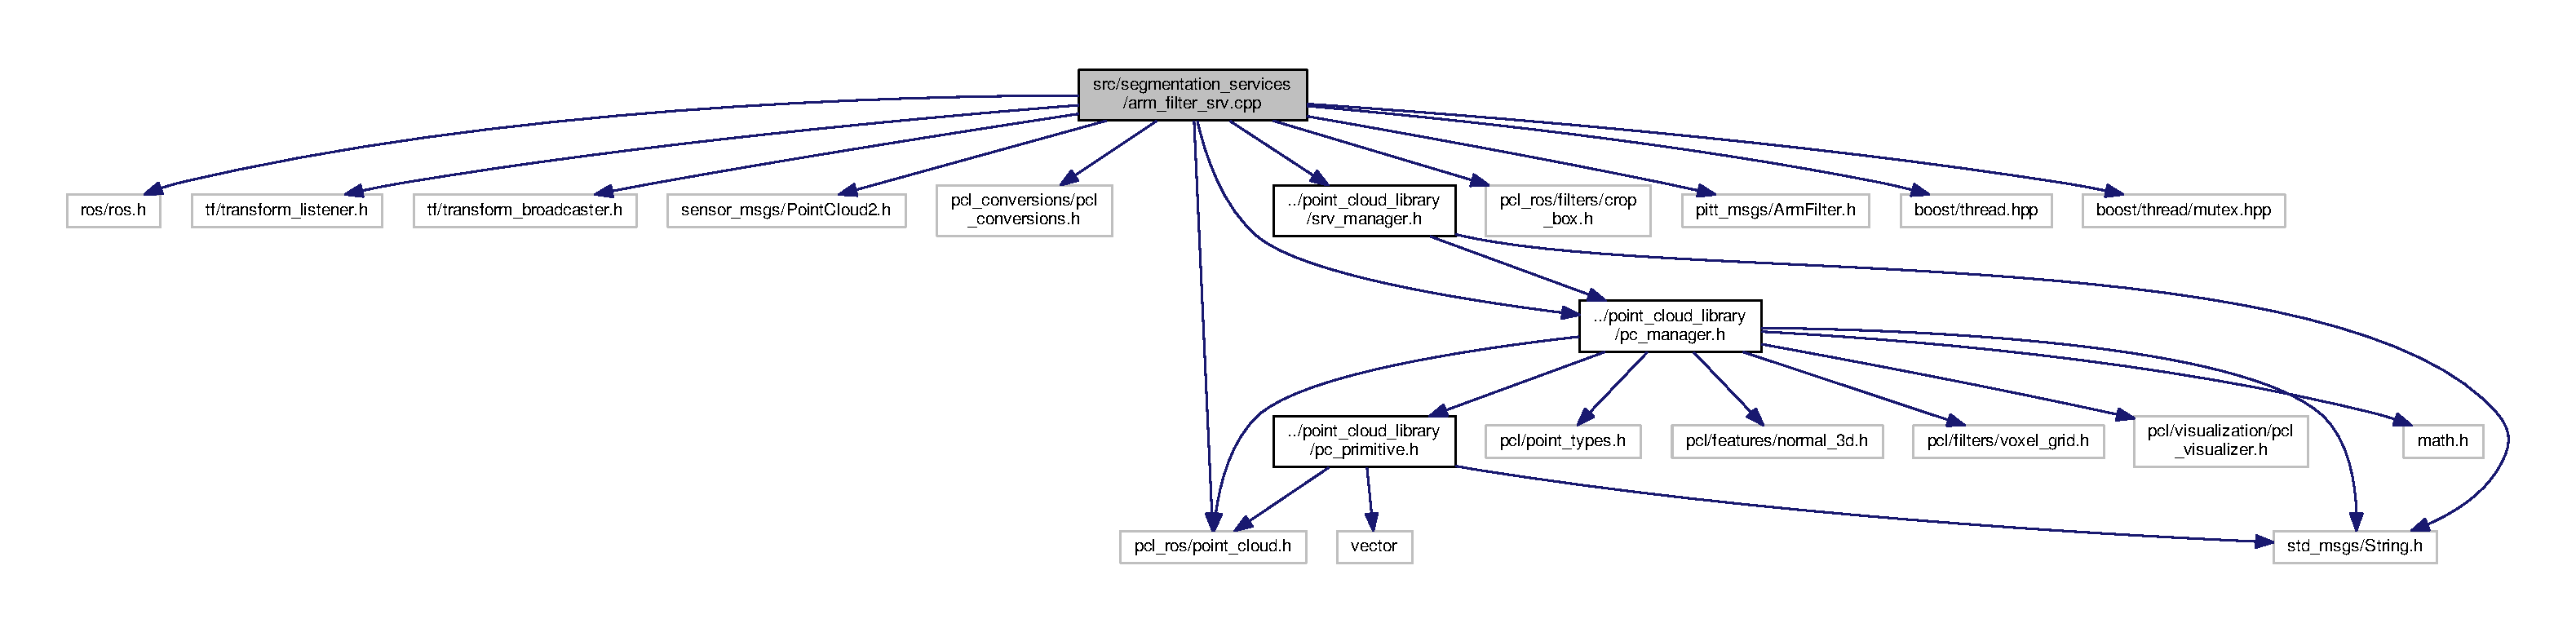
\includegraphics[width=350pt]{arm__filter__srv_8cpp__incl}
\end{center}
\end{figure}
\subsection*{Functions}
\begin{DoxyCompactItemize}
\item 
\hyperlink{pc__primitive_8h_aa14a240c8d999c4f56133c0f70e88783}{P\-C\-L\-Cloud\-Ptr} \hyperlink{arm__filter__srv_8cpp_a974bd4721d13dc5fa4bd9608eca657db}{input\-Cloud} (new \hyperlink{pc__primitive_8h_a02a7c0cdfcd324f1b5b87ce549fdbe10}{P\-C\-L\-Cloud})
\item 
\hyperlink{pc__primitive_8h_aa14a240c8d999c4f56133c0f70e88783}{P\-C\-L\-Cloud\-Ptr} \hyperlink{arm__filter__srv_8cpp_aa4b6c2d24b5c4911d3ebbb967999a82b}{output\-Cloud1} (new \hyperlink{pc__primitive_8h_a02a7c0cdfcd324f1b5b87ce549fdbe10}{P\-C\-L\-Cloud})
\item 
\hyperlink{pc__primitive_8h_aa14a240c8d999c4f56133c0f70e88783}{P\-C\-L\-Cloud\-Ptr} \hyperlink{arm__filter__srv_8cpp_ae3aee46e0451f823a21c451fd9c8ac25}{output\-Cloud2} (new \hyperlink{pc__primitive_8h_a02a7c0cdfcd324f1b5b87ce549fdbe10}{P\-C\-L\-Cloud})
\item 
\hyperlink{pc__primitive_8h_aa14a240c8d999c4f56133c0f70e88783}{P\-C\-L\-Cloud\-Ptr} \hyperlink{arm__filter__srv_8cpp_a5c266d98a960f6334baad8956a4569c5}{output\-Cloud3} (new \hyperlink{pc__primitive_8h_a02a7c0cdfcd324f1b5b87ce549fdbe10}{P\-C\-L\-Cloud})
\item 
\hyperlink{pc__primitive_8h_aa14a240c8d999c4f56133c0f70e88783}{P\-C\-L\-Cloud\-Ptr} \hyperlink{arm__filter__srv_8cpp_a7e3b25c3b127afe65902cc9673c1d8cd}{output\-Cloud4} (new \hyperlink{pc__primitive_8h_a02a7c0cdfcd324f1b5b87ce549fdbe10}{P\-C\-L\-Cloud})
\item 
void \hyperlink{arm__filter__srv_8cpp_aca73ab26cae45b4b998a3cca9e4f75bc}{vis\-Spin} ()
\item 
\hyperlink{pc__primitive_8h_aa14a240c8d999c4f56133c0f70e88783}{P\-C\-L\-Cloud\-Ptr} \hyperlink{arm__filter__srv_8cpp_a3229044f42efe1f63799bf085f25e465}{arm\-Filtering} (\hyperlink{pc__primitive_8h_aa14a240c8d999c4f56133c0f70e88783}{P\-C\-L\-Cloud\-Ptr} original, Vector4f min\-Values, Vector4f max\-Values, Stamped\-Transform frame)
\item 
Vector4f \hyperlink{arm__filter__srv_8cpp_a5cf0837efbabf7b72d1097947627893b}{generate\-Box\-Vector} (vector$<$ float $>$ vec)
\item 
bool \hyperlink{arm__filter__srv_8cpp_a6afacda051b868ce7950d386882d76ce}{filter} (Arm\-Filter\-Request \&input, Arm\-Filter\-Response \&output)
\item 
int \hyperlink{arm__filter__srv_8cpp_a3c04138a5bfe5d72780bb7e82a18e627}{main} (int argc, char $\ast$$\ast$argv)
\end{DoxyCompactItemize}
\subsection*{Variables}
\begin{DoxyCompactItemize}
\item 
const float \hyperlink{arm__filter__srv_8cpp_a971d8e3e736e997485729c43c2c672db}{D\-E\-F\-A\-U\-L\-T\-\_\-\-P\-A\-R\-A\-M\-\_\-\-A\-R\-M\-\_\-\-S\-R\-V\-\_\-\-M\-I\-N\-\_\-\-F\-O\-R\-E\-A\-R\-M\-\_\-\-B\-O\-X} \mbox{[}$\,$\mbox{]} = \{ -\/0.\-040f, -\/0.\-120f, -\/0.\-190f\}
\item 
const float \hyperlink{arm__filter__srv_8cpp_aa17660d438631874e727d0963174ce2a}{D\-E\-F\-A\-U\-L\-T\-\_\-\-P\-A\-R\-A\-M\-\_\-\-A\-R\-M\-\_\-\-S\-R\-V\-\_\-\-M\-A\-X\-\_\-\-F\-O\-R\-E\-A\-R\-M\-\_\-\-B\-O\-X} \mbox{[}$\,$\mbox{]} = \{ 0.\-340f, 0.\-120f, 0.\-105f\}
\item 
const float \hyperlink{arm__filter__srv_8cpp_a797cc99d83ba96165db23a53940bafcd}{D\-E\-F\-A\-U\-L\-T\-\_\-\-P\-A\-R\-A\-M\-\_\-\-A\-R\-M\-\_\-\-S\-R\-V\-\_\-\-M\-I\-N\-\_\-\-E\-L\-B\-O\-W\-\_\-\-B\-O\-X} \mbox{[}$\,$\mbox{]} = \{ -\/0.\-090f, -\/0.\-135f, -\/0.\-160f\}
\item 
const float \hyperlink{arm__filter__srv_8cpp_a791c9a7f284cd7ec10995be1f5072744}{D\-E\-F\-A\-U\-L\-T\-\_\-\-P\-A\-R\-A\-M\-\_\-\-A\-R\-M\-\_\-\-S\-R\-V\-\_\-\-M\-A\-X\-\_\-\-E\-L\-B\-O\-W\-\_\-\-B\-O\-X} \mbox{[}$\,$\mbox{]} = \{ 0.\-440f, 0.\-135f, 0.\-110f\}
\item 
const Duration \hyperlink{arm__filter__srv_8cpp_a3e053a77ab85888a3853cee24610ddf4}{W\-A\-I\-T\-\_\-\-F\-O\-R\-\_\-\-T\-F\-\_\-\-T\-I\-M\-E\-\_\-\-O\-U\-T} = Duration( \hyperlink{namespacesrvm_a6debc60d19f8c5cfe2e7746da001f0d1}{srvm\-::\-D\-E\-F\-A\-U\-L\-T\-\_\-\-T\-F\-\_\-\-W\-A\-I\-T\-\_\-\-S\-E\-C\-O\-N\-D\-S})
\item 
Stamped\-Transform \hyperlink{arm__filter__srv_8cpp_a4a19c359b6d406082f134aba17d3e5ea}{left\-Forearm\-Camera\-Tansf}
\item 
Stamped\-Transform \hyperlink{arm__filter__srv_8cpp_a7522b3883c33cecc896e8ccf4f48558d}{right\-Forearm\-Camera\-Tansf}
\item 
Stamped\-Transform \hyperlink{arm__filter__srv_8cpp_a88cbfe2fdbf19a20a88cd96735e7590b}{left\-Elbow\-Camera\-Tansf}
\item 
Stamped\-Transform \hyperlink{arm__filter__srv_8cpp_abfad2066863e6d2f21ba1f98106087ca}{right\-Elbow\-Camera\-Tansf}
\item 
bool \hyperlink{arm__filter__srv_8cpp_a163bafbb51ee2789c7dcc991b5a1e903}{tf\-Error} = false
\item 
bool \hyperlink{arm__filter__srv_8cpp_a13dc5bbf0a8964f809cb5d647a02f008}{show\-Clouds}
\item 
boost\-::shared\-\_\-ptr\\*
$<$ \hyperlink{pc__manager_8h_a38c805dbc7ad6f06109b85c8e540817a}{visualization\-::\-P\-C\-L\-Visualizer} $>$ \hyperlink{arm__filter__srv_8cpp_a6c2d87234fca8dcca11f888098558986}{vis}
\item 
boost\-::thread \hyperlink{arm__filter__srv_8cpp_ab83e6219895a4d26706c0d858f8ec288}{vis\-\_\-thread}
\item 
boost\-::mutex \hyperlink{arm__filter__srv_8cpp_a0dc8882293908d9c8cc15f76a2a49588}{vis\-\_\-mutex}
\item 
string \hyperlink{arm__filter__srv_8cpp_a484374fe771cd860a2ea9f9feda68905}{log\-\_\-str\-\_\-depth} = \char`\"{}Loading...\char`\"{}
\end{DoxyCompactItemize}


\subsection{Function Documentation}
\hypertarget{arm__filter__srv_8cpp_a3229044f42efe1f63799bf085f25e465}{\index{arm\-\_\-filter\-\_\-srv.\-cpp@{arm\-\_\-filter\-\_\-srv.\-cpp}!arm\-Filtering@{arm\-Filtering}}
\index{arm\-Filtering@{arm\-Filtering}!arm_filter_srv.cpp@{arm\-\_\-filter\-\_\-srv.\-cpp}}
\subsubsection[{arm\-Filtering}]{\setlength{\rightskip}{0pt plus 5cm}{\bf P\-C\-L\-Cloud\-Ptr} arm\-Filtering (
\begin{DoxyParamCaption}
\item[{{\bf P\-C\-L\-Cloud\-Ptr}}]{original, }
\item[{Vector4f}]{min\-Values, }
\item[{Vector4f}]{max\-Values, }
\item[{Stamped\-Transform}]{frame}
\end{DoxyParamCaption}
)}}\label{arm__filter__srv_8cpp_a3229044f42efe1f63799bf085f25e465}


Definition at line 66 of file arm\-\_\-filter\-\_\-srv.\-cpp.



Referenced by filter().

\hypertarget{arm__filter__srv_8cpp_a6afacda051b868ce7950d386882d76ce}{\index{arm\-\_\-filter\-\_\-srv.\-cpp@{arm\-\_\-filter\-\_\-srv.\-cpp}!filter@{filter}}
\index{filter@{filter}!arm_filter_srv.cpp@{arm\-\_\-filter\-\_\-srv.\-cpp}}
\subsubsection[{filter}]{\setlength{\rightskip}{0pt plus 5cm}bool filter (
\begin{DoxyParamCaption}
\item[{Arm\-Filter\-Request \&}]{input, }
\item[{Arm\-Filter\-Response \&}]{output}
\end{DoxyParamCaption}
)}}\label{arm__filter__srv_8cpp_a6afacda051b868ce7950d386882d76ce}


Definition at line 112 of file arm\-\_\-filter\-\_\-srv.\-cpp.



References arm\-Filtering(), D\-E\-F\-A\-U\-L\-T\-\_\-\-P\-A\-R\-A\-M\-\_\-\-A\-R\-M\-\_\-\-S\-R\-V\-\_\-\-M\-A\-X\-\_\-\-E\-L\-B\-O\-W\-\_\-\-B\-O\-X, D\-E\-F\-A\-U\-L\-T\-\_\-\-P\-A\-R\-A\-M\-\_\-\-A\-R\-M\-\_\-\-S\-R\-V\-\_\-\-M\-A\-X\-\_\-\-F\-O\-R\-E\-A\-R\-M\-\_\-\-B\-O\-X, D\-E\-F\-A\-U\-L\-T\-\_\-\-P\-A\-R\-A\-M\-\_\-\-A\-R\-M\-\_\-\-S\-R\-V\-\_\-\-M\-I\-N\-\_\-\-E\-L\-B\-O\-W\-\_\-\-B\-O\-X, D\-E\-F\-A\-U\-L\-T\-\_\-\-P\-A\-R\-A\-M\-\_\-\-A\-R\-M\-\_\-\-S\-R\-V\-\_\-\-M\-I\-N\-\_\-\-F\-O\-R\-E\-A\-R\-M\-\_\-\-B\-O\-X, generate\-Box\-Vector(), srvm\-::get\-Array\-To\-Print(), srvm\-::get\-Service3\-D\-Array\-Parameter(), input\-Cloud(), left\-Elbow\-Camera\-Tansf, left\-Forearm\-Camera\-Tansf, log\-\_\-str\-\_\-depth, output\-Cloud1(), output\-Cloud2(), output\-Cloud3(), output\-Cloud4(), right\-Elbow\-Camera\-Tansf, right\-Forearm\-Camera\-Tansf, show\-Clouds, tf\-Error, vis, and vis\-\_\-mutex.



Referenced by main().



Here is the call graph for this function\-:
\nopagebreak
\begin{figure}[H]
\begin{center}
\leavevmode
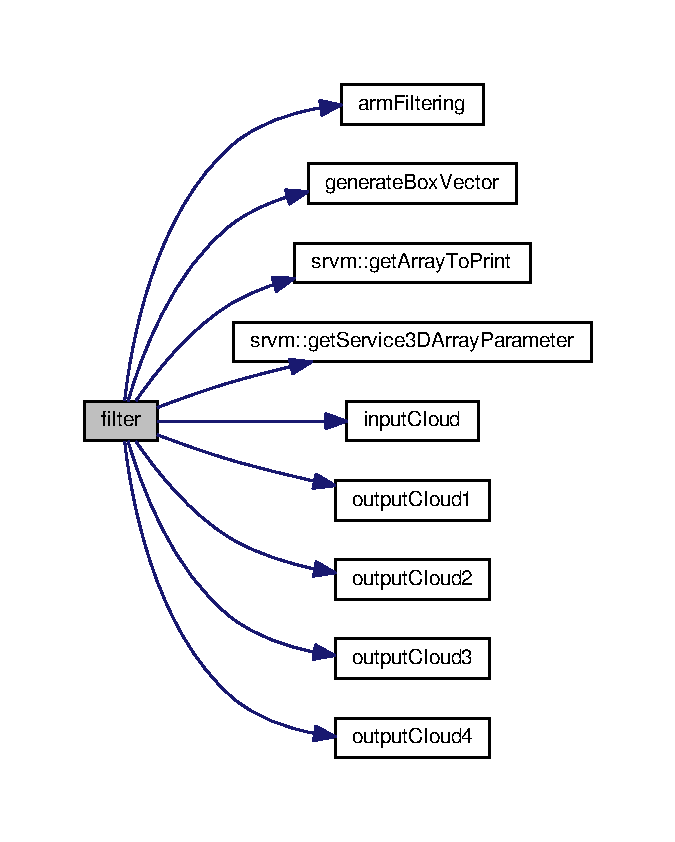
\includegraphics[width=324pt]{arm__filter__srv_8cpp_a6afacda051b868ce7950d386882d76ce_cgraph}
\end{center}
\end{figure}


\hypertarget{arm__filter__srv_8cpp_a5cf0837efbabf7b72d1097947627893b}{\index{arm\-\_\-filter\-\_\-srv.\-cpp@{arm\-\_\-filter\-\_\-srv.\-cpp}!generate\-Box\-Vector@{generate\-Box\-Vector}}
\index{generate\-Box\-Vector@{generate\-Box\-Vector}!arm_filter_srv.cpp@{arm\-\_\-filter\-\_\-srv.\-cpp}}
\subsubsection[{generate\-Box\-Vector}]{\setlength{\rightskip}{0pt plus 5cm}Vector4f generate\-Box\-Vector (
\begin{DoxyParamCaption}
\item[{vector$<$ float $>$}]{vec}
\end{DoxyParamCaption}
)}}\label{arm__filter__srv_8cpp_a5cf0837efbabf7b72d1097947627893b}


Definition at line 105 of file arm\-\_\-filter\-\_\-srv.\-cpp.



Referenced by filter().

\hypertarget{arm__filter__srv_8cpp_a974bd4721d13dc5fa4bd9608eca657db}{\index{arm\-\_\-filter\-\_\-srv.\-cpp@{arm\-\_\-filter\-\_\-srv.\-cpp}!input\-Cloud@{input\-Cloud}}
\index{input\-Cloud@{input\-Cloud}!arm_filter_srv.cpp@{arm\-\_\-filter\-\_\-srv.\-cpp}}
\subsubsection[{input\-Cloud}]{\setlength{\rightskip}{0pt plus 5cm}{\bf P\-C\-L\-Cloud\-Ptr} input\-Cloud (
\begin{DoxyParamCaption}
\item[{new}]{P\-C\-L\-Cloud}
\end{DoxyParamCaption}
)}}\label{arm__filter__srv_8cpp_a974bd4721d13dc5fa4bd9608eca657db}


Referenced by filter().

\hypertarget{arm__filter__srv_8cpp_a3c04138a5bfe5d72780bb7e82a18e627}{\index{arm\-\_\-filter\-\_\-srv.\-cpp@{arm\-\_\-filter\-\_\-srv.\-cpp}!main@{main}}
\index{main@{main}!arm_filter_srv.cpp@{arm\-\_\-filter\-\_\-srv.\-cpp}}
\subsubsection[{main}]{\setlength{\rightskip}{0pt plus 5cm}int main (
\begin{DoxyParamCaption}
\item[{int}]{argc, }
\item[{char $\ast$$\ast$}]{argv}
\end{DoxyParamCaption}
)}}\label{arm__filter__srv_8cpp_a3c04138a5bfe5d72780bb7e82a18e627}


Definition at line 183 of file arm\-\_\-filter\-\_\-srv.\-cpp.



References srvm\-::\-D\-E\-F\-A\-U\-L\-T\-\_\-\-P\-A\-R\-A\-M\-\_\-\-A\-R\-M\-\_\-\-S\-R\-V\-\_\-\-C\-A\-M\-E\-R\-A\-\_\-\-F\-R\-A\-M\-E, srvm\-::\-D\-E\-F\-A\-U\-L\-T\-\_\-\-P\-A\-R\-A\-M\-\_\-\-A\-R\-M\-\_\-\-S\-R\-V\-\_\-\-L\-E\-F\-T\-\_\-\-E\-L\-B\-O\-W\-\_\-\-F\-R\-A\-M\-E, srvm\-::\-D\-E\-F\-A\-U\-L\-T\-\_\-\-P\-A\-R\-A\-M\-\_\-\-A\-R\-M\-\_\-\-S\-R\-V\-\_\-\-L\-E\-F\-T\-\_\-\-F\-O\-R\-E\-A\-R\-M\-\_\-\-F\-R\-A\-M\-E, srvm\-::\-D\-E\-F\-A\-U\-L\-T\-\_\-\-P\-A\-R\-A\-M\-\_\-\-A\-R\-M\-\_\-\-S\-R\-V\-\_\-\-R\-I\-G\-H\-T\-\_\-\-E\-L\-B\-O\-W\-\_\-\-F\-R\-A\-M\-E, srvm\-::\-D\-E\-F\-A\-U\-L\-T\-\_\-\-P\-A\-R\-A\-M\-\_\-\-A\-R\-M\-\_\-\-S\-R\-V\-\_\-\-R\-I\-G\-H\-T\-\_\-\-F\-O\-R\-E\-A\-R\-M\-\_\-\-F\-R\-A\-M\-E, srvm\-::\-D\-E\-F\-A\-U\-L\-T\-\_\-\-P\-A\-R\-A\-M\-\_\-\-A\-R\-M\-\_\-\-S\-R\-V\-\_\-\-S\-H\-O\-W\-\_\-\-C\-L\-O\-U\-D\-S, filter(), srvm\-::get\-Bool\-Ptr\-Parameter(), srvm\-::get\-String\-Ptr\-Parameter(), left\-Elbow\-Camera\-Tansf, left\-Forearm\-Camera\-Tansf, log\-\_\-str\-\_\-depth, right\-Elbow\-Camera\-Tansf, right\-Forearm\-Camera\-Tansf, show\-Clouds, srvm\-::\-S\-R\-V\-\_\-\-N\-A\-M\-E\-\_\-\-A\-R\-M\-\_\-\-F\-I\-L\-T\-E\-R, tf\-Error, vis, vis\-\_\-thread, vis\-Spin(), and W\-A\-I\-T\-\_\-\-F\-O\-R\-\_\-\-T\-F\-\_\-\-T\-I\-M\-E\-\_\-\-O\-U\-T.



Here is the call graph for this function\-:
\nopagebreak
\begin{figure}[H]
\begin{center}
\leavevmode
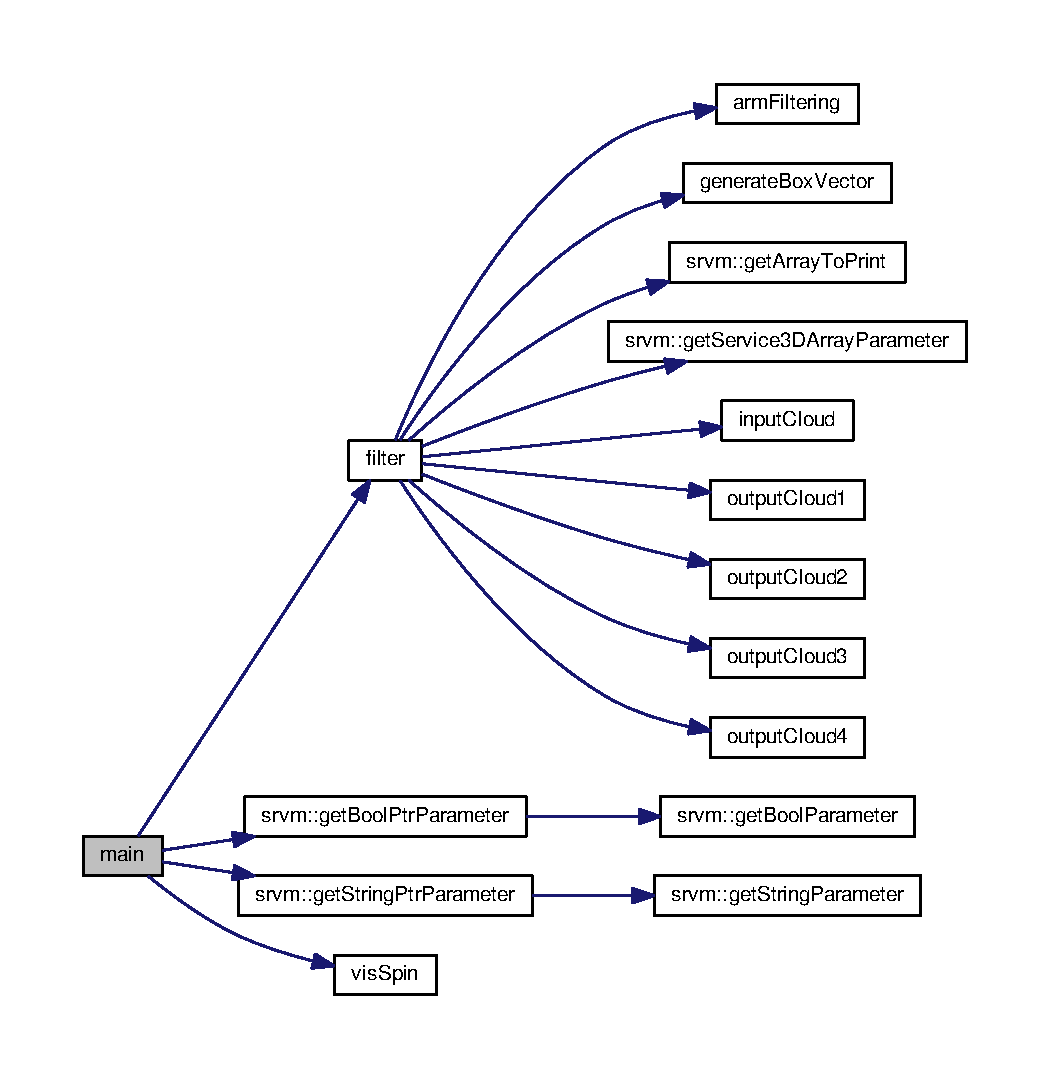
\includegraphics[width=350pt]{arm__filter__srv_8cpp_a3c04138a5bfe5d72780bb7e82a18e627_cgraph}
\end{center}
\end{figure}


\hypertarget{arm__filter__srv_8cpp_aa4b6c2d24b5c4911d3ebbb967999a82b}{\index{arm\-\_\-filter\-\_\-srv.\-cpp@{arm\-\_\-filter\-\_\-srv.\-cpp}!output\-Cloud1@{output\-Cloud1}}
\index{output\-Cloud1@{output\-Cloud1}!arm_filter_srv.cpp@{arm\-\_\-filter\-\_\-srv.\-cpp}}
\subsubsection[{output\-Cloud1}]{\setlength{\rightskip}{0pt plus 5cm}{\bf P\-C\-L\-Cloud\-Ptr} output\-Cloud1 (
\begin{DoxyParamCaption}
\item[{new}]{P\-C\-L\-Cloud}
\end{DoxyParamCaption}
)}}\label{arm__filter__srv_8cpp_aa4b6c2d24b5c4911d3ebbb967999a82b}


Referenced by filter().

\hypertarget{arm__filter__srv_8cpp_ae3aee46e0451f823a21c451fd9c8ac25}{\index{arm\-\_\-filter\-\_\-srv.\-cpp@{arm\-\_\-filter\-\_\-srv.\-cpp}!output\-Cloud2@{output\-Cloud2}}
\index{output\-Cloud2@{output\-Cloud2}!arm_filter_srv.cpp@{arm\-\_\-filter\-\_\-srv.\-cpp}}
\subsubsection[{output\-Cloud2}]{\setlength{\rightskip}{0pt plus 5cm}{\bf P\-C\-L\-Cloud\-Ptr} output\-Cloud2 (
\begin{DoxyParamCaption}
\item[{new}]{P\-C\-L\-Cloud}
\end{DoxyParamCaption}
)}}\label{arm__filter__srv_8cpp_ae3aee46e0451f823a21c451fd9c8ac25}


Referenced by filter().

\hypertarget{arm__filter__srv_8cpp_a5c266d98a960f6334baad8956a4569c5}{\index{arm\-\_\-filter\-\_\-srv.\-cpp@{arm\-\_\-filter\-\_\-srv.\-cpp}!output\-Cloud3@{output\-Cloud3}}
\index{output\-Cloud3@{output\-Cloud3}!arm_filter_srv.cpp@{arm\-\_\-filter\-\_\-srv.\-cpp}}
\subsubsection[{output\-Cloud3}]{\setlength{\rightskip}{0pt plus 5cm}{\bf P\-C\-L\-Cloud\-Ptr} output\-Cloud3 (
\begin{DoxyParamCaption}
\item[{new}]{P\-C\-L\-Cloud}
\end{DoxyParamCaption}
)}}\label{arm__filter__srv_8cpp_a5c266d98a960f6334baad8956a4569c5}


Referenced by filter().

\hypertarget{arm__filter__srv_8cpp_a7e3b25c3b127afe65902cc9673c1d8cd}{\index{arm\-\_\-filter\-\_\-srv.\-cpp@{arm\-\_\-filter\-\_\-srv.\-cpp}!output\-Cloud4@{output\-Cloud4}}
\index{output\-Cloud4@{output\-Cloud4}!arm_filter_srv.cpp@{arm\-\_\-filter\-\_\-srv.\-cpp}}
\subsubsection[{output\-Cloud4}]{\setlength{\rightskip}{0pt plus 5cm}{\bf P\-C\-L\-Cloud\-Ptr} output\-Cloud4 (
\begin{DoxyParamCaption}
\item[{new}]{P\-C\-L\-Cloud}
\end{DoxyParamCaption}
)}}\label{arm__filter__srv_8cpp_a7e3b25c3b127afe65902cc9673c1d8cd}


Referenced by filter().

\hypertarget{arm__filter__srv_8cpp_aca73ab26cae45b4b998a3cca9e4f75bc}{\index{arm\-\_\-filter\-\_\-srv.\-cpp@{arm\-\_\-filter\-\_\-srv.\-cpp}!vis\-Spin@{vis\-Spin}}
\index{vis\-Spin@{vis\-Spin}!arm_filter_srv.cpp@{arm\-\_\-filter\-\_\-srv.\-cpp}}
\subsubsection[{vis\-Spin}]{\setlength{\rightskip}{0pt plus 5cm}void vis\-Spin (
\begin{DoxyParamCaption}
{}
\end{DoxyParamCaption}
)}}\label{arm__filter__srv_8cpp_aca73ab26cae45b4b998a3cca9e4f75bc}


Definition at line 57 of file arm\-\_\-filter\-\_\-srv.\-cpp.



References vis, and vis\-\_\-mutex.



Referenced by main().



\subsection{Variable Documentation}
\hypertarget{arm__filter__srv_8cpp_a791c9a7f284cd7ec10995be1f5072744}{\index{arm\-\_\-filter\-\_\-srv.\-cpp@{arm\-\_\-filter\-\_\-srv.\-cpp}!D\-E\-F\-A\-U\-L\-T\-\_\-\-P\-A\-R\-A\-M\-\_\-\-A\-R\-M\-\_\-\-S\-R\-V\-\_\-\-M\-A\-X\-\_\-\-E\-L\-B\-O\-W\-\_\-\-B\-O\-X@{D\-E\-F\-A\-U\-L\-T\-\_\-\-P\-A\-R\-A\-M\-\_\-\-A\-R\-M\-\_\-\-S\-R\-V\-\_\-\-M\-A\-X\-\_\-\-E\-L\-B\-O\-W\-\_\-\-B\-O\-X}}
\index{D\-E\-F\-A\-U\-L\-T\-\_\-\-P\-A\-R\-A\-M\-\_\-\-A\-R\-M\-\_\-\-S\-R\-V\-\_\-\-M\-A\-X\-\_\-\-E\-L\-B\-O\-W\-\_\-\-B\-O\-X@{D\-E\-F\-A\-U\-L\-T\-\_\-\-P\-A\-R\-A\-M\-\_\-\-A\-R\-M\-\_\-\-S\-R\-V\-\_\-\-M\-A\-X\-\_\-\-E\-L\-B\-O\-W\-\_\-\-B\-O\-X}!arm_filter_srv.cpp@{arm\-\_\-filter\-\_\-srv.\-cpp}}
\subsubsection[{D\-E\-F\-A\-U\-L\-T\-\_\-\-P\-A\-R\-A\-M\-\_\-\-A\-R\-M\-\_\-\-S\-R\-V\-\_\-\-M\-A\-X\-\_\-\-E\-L\-B\-O\-W\-\_\-\-B\-O\-X}]{\setlength{\rightskip}{0pt plus 5cm}const float D\-E\-F\-A\-U\-L\-T\-\_\-\-P\-A\-R\-A\-M\-\_\-\-A\-R\-M\-\_\-\-S\-R\-V\-\_\-\-M\-A\-X\-\_\-\-E\-L\-B\-O\-W\-\_\-\-B\-O\-X\mbox{[}$\,$\mbox{]} = \{ 0.\-440f, 0.\-135f, 0.\-110f\}}}\label{arm__filter__srv_8cpp_a791c9a7f284cd7ec10995be1f5072744}


Definition at line 35 of file arm\-\_\-filter\-\_\-srv.\-cpp.



Referenced by filter().

\hypertarget{arm__filter__srv_8cpp_aa17660d438631874e727d0963174ce2a}{\index{arm\-\_\-filter\-\_\-srv.\-cpp@{arm\-\_\-filter\-\_\-srv.\-cpp}!D\-E\-F\-A\-U\-L\-T\-\_\-\-P\-A\-R\-A\-M\-\_\-\-A\-R\-M\-\_\-\-S\-R\-V\-\_\-\-M\-A\-X\-\_\-\-F\-O\-R\-E\-A\-R\-M\-\_\-\-B\-O\-X@{D\-E\-F\-A\-U\-L\-T\-\_\-\-P\-A\-R\-A\-M\-\_\-\-A\-R\-M\-\_\-\-S\-R\-V\-\_\-\-M\-A\-X\-\_\-\-F\-O\-R\-E\-A\-R\-M\-\_\-\-B\-O\-X}}
\index{D\-E\-F\-A\-U\-L\-T\-\_\-\-P\-A\-R\-A\-M\-\_\-\-A\-R\-M\-\_\-\-S\-R\-V\-\_\-\-M\-A\-X\-\_\-\-F\-O\-R\-E\-A\-R\-M\-\_\-\-B\-O\-X@{D\-E\-F\-A\-U\-L\-T\-\_\-\-P\-A\-R\-A\-M\-\_\-\-A\-R\-M\-\_\-\-S\-R\-V\-\_\-\-M\-A\-X\-\_\-\-F\-O\-R\-E\-A\-R\-M\-\_\-\-B\-O\-X}!arm_filter_srv.cpp@{arm\-\_\-filter\-\_\-srv.\-cpp}}
\subsubsection[{D\-E\-F\-A\-U\-L\-T\-\_\-\-P\-A\-R\-A\-M\-\_\-\-A\-R\-M\-\_\-\-S\-R\-V\-\_\-\-M\-A\-X\-\_\-\-F\-O\-R\-E\-A\-R\-M\-\_\-\-B\-O\-X}]{\setlength{\rightskip}{0pt plus 5cm}const float D\-E\-F\-A\-U\-L\-T\-\_\-\-P\-A\-R\-A\-M\-\_\-\-A\-R\-M\-\_\-\-S\-R\-V\-\_\-\-M\-A\-X\-\_\-\-F\-O\-R\-E\-A\-R\-M\-\_\-\-B\-O\-X\mbox{[}$\,$\mbox{]} = \{ 0.\-340f, 0.\-120f, 0.\-105f\}}}\label{arm__filter__srv_8cpp_aa17660d438631874e727d0963174ce2a}


Definition at line 33 of file arm\-\_\-filter\-\_\-srv.\-cpp.



Referenced by filter().

\hypertarget{arm__filter__srv_8cpp_a797cc99d83ba96165db23a53940bafcd}{\index{arm\-\_\-filter\-\_\-srv.\-cpp@{arm\-\_\-filter\-\_\-srv.\-cpp}!D\-E\-F\-A\-U\-L\-T\-\_\-\-P\-A\-R\-A\-M\-\_\-\-A\-R\-M\-\_\-\-S\-R\-V\-\_\-\-M\-I\-N\-\_\-\-E\-L\-B\-O\-W\-\_\-\-B\-O\-X@{D\-E\-F\-A\-U\-L\-T\-\_\-\-P\-A\-R\-A\-M\-\_\-\-A\-R\-M\-\_\-\-S\-R\-V\-\_\-\-M\-I\-N\-\_\-\-E\-L\-B\-O\-W\-\_\-\-B\-O\-X}}
\index{D\-E\-F\-A\-U\-L\-T\-\_\-\-P\-A\-R\-A\-M\-\_\-\-A\-R\-M\-\_\-\-S\-R\-V\-\_\-\-M\-I\-N\-\_\-\-E\-L\-B\-O\-W\-\_\-\-B\-O\-X@{D\-E\-F\-A\-U\-L\-T\-\_\-\-P\-A\-R\-A\-M\-\_\-\-A\-R\-M\-\_\-\-S\-R\-V\-\_\-\-M\-I\-N\-\_\-\-E\-L\-B\-O\-W\-\_\-\-B\-O\-X}!arm_filter_srv.cpp@{arm\-\_\-filter\-\_\-srv.\-cpp}}
\subsubsection[{D\-E\-F\-A\-U\-L\-T\-\_\-\-P\-A\-R\-A\-M\-\_\-\-A\-R\-M\-\_\-\-S\-R\-V\-\_\-\-M\-I\-N\-\_\-\-E\-L\-B\-O\-W\-\_\-\-B\-O\-X}]{\setlength{\rightskip}{0pt plus 5cm}const float D\-E\-F\-A\-U\-L\-T\-\_\-\-P\-A\-R\-A\-M\-\_\-\-A\-R\-M\-\_\-\-S\-R\-V\-\_\-\-M\-I\-N\-\_\-\-E\-L\-B\-O\-W\-\_\-\-B\-O\-X\mbox{[}$\,$\mbox{]} = \{ -\/0.\-090f, -\/0.\-135f, -\/0.\-160f\}}}\label{arm__filter__srv_8cpp_a797cc99d83ba96165db23a53940bafcd}


Definition at line 34 of file arm\-\_\-filter\-\_\-srv.\-cpp.



Referenced by filter().

\hypertarget{arm__filter__srv_8cpp_a971d8e3e736e997485729c43c2c672db}{\index{arm\-\_\-filter\-\_\-srv.\-cpp@{arm\-\_\-filter\-\_\-srv.\-cpp}!D\-E\-F\-A\-U\-L\-T\-\_\-\-P\-A\-R\-A\-M\-\_\-\-A\-R\-M\-\_\-\-S\-R\-V\-\_\-\-M\-I\-N\-\_\-\-F\-O\-R\-E\-A\-R\-M\-\_\-\-B\-O\-X@{D\-E\-F\-A\-U\-L\-T\-\_\-\-P\-A\-R\-A\-M\-\_\-\-A\-R\-M\-\_\-\-S\-R\-V\-\_\-\-M\-I\-N\-\_\-\-F\-O\-R\-E\-A\-R\-M\-\_\-\-B\-O\-X}}
\index{D\-E\-F\-A\-U\-L\-T\-\_\-\-P\-A\-R\-A\-M\-\_\-\-A\-R\-M\-\_\-\-S\-R\-V\-\_\-\-M\-I\-N\-\_\-\-F\-O\-R\-E\-A\-R\-M\-\_\-\-B\-O\-X@{D\-E\-F\-A\-U\-L\-T\-\_\-\-P\-A\-R\-A\-M\-\_\-\-A\-R\-M\-\_\-\-S\-R\-V\-\_\-\-M\-I\-N\-\_\-\-F\-O\-R\-E\-A\-R\-M\-\_\-\-B\-O\-X}!arm_filter_srv.cpp@{arm\-\_\-filter\-\_\-srv.\-cpp}}
\subsubsection[{D\-E\-F\-A\-U\-L\-T\-\_\-\-P\-A\-R\-A\-M\-\_\-\-A\-R\-M\-\_\-\-S\-R\-V\-\_\-\-M\-I\-N\-\_\-\-F\-O\-R\-E\-A\-R\-M\-\_\-\-B\-O\-X}]{\setlength{\rightskip}{0pt plus 5cm}const float D\-E\-F\-A\-U\-L\-T\-\_\-\-P\-A\-R\-A\-M\-\_\-\-A\-R\-M\-\_\-\-S\-R\-V\-\_\-\-M\-I\-N\-\_\-\-F\-O\-R\-E\-A\-R\-M\-\_\-\-B\-O\-X\mbox{[}$\,$\mbox{]} = \{ -\/0.\-040f, -\/0.\-120f, -\/0.\-190f\}}}\label{arm__filter__srv_8cpp_a971d8e3e736e997485729c43c2c672db}


Definition at line 32 of file arm\-\_\-filter\-\_\-srv.\-cpp.



Referenced by filter().

\hypertarget{arm__filter__srv_8cpp_a88cbfe2fdbf19a20a88cd96735e7590b}{\index{arm\-\_\-filter\-\_\-srv.\-cpp@{arm\-\_\-filter\-\_\-srv.\-cpp}!left\-Elbow\-Camera\-Tansf@{left\-Elbow\-Camera\-Tansf}}
\index{left\-Elbow\-Camera\-Tansf@{left\-Elbow\-Camera\-Tansf}!arm_filter_srv.cpp@{arm\-\_\-filter\-\_\-srv.\-cpp}}
\subsubsection[{left\-Elbow\-Camera\-Tansf}]{\setlength{\rightskip}{0pt plus 5cm}Stamped\-Transform left\-Elbow\-Camera\-Tansf}}\label{arm__filter__srv_8cpp_a88cbfe2fdbf19a20a88cd96735e7590b}


Definition at line 40 of file arm\-\_\-filter\-\_\-srv.\-cpp.



Referenced by filter(), and main().

\hypertarget{arm__filter__srv_8cpp_a4a19c359b6d406082f134aba17d3e5ea}{\index{arm\-\_\-filter\-\_\-srv.\-cpp@{arm\-\_\-filter\-\_\-srv.\-cpp}!left\-Forearm\-Camera\-Tansf@{left\-Forearm\-Camera\-Tansf}}
\index{left\-Forearm\-Camera\-Tansf@{left\-Forearm\-Camera\-Tansf}!arm_filter_srv.cpp@{arm\-\_\-filter\-\_\-srv.\-cpp}}
\subsubsection[{left\-Forearm\-Camera\-Tansf}]{\setlength{\rightskip}{0pt plus 5cm}Stamped\-Transform left\-Forearm\-Camera\-Tansf}}\label{arm__filter__srv_8cpp_a4a19c359b6d406082f134aba17d3e5ea}


Definition at line 40 of file arm\-\_\-filter\-\_\-srv.\-cpp.



Referenced by filter(), and main().

\hypertarget{arm__filter__srv_8cpp_a484374fe771cd860a2ea9f9feda68905}{\index{arm\-\_\-filter\-\_\-srv.\-cpp@{arm\-\_\-filter\-\_\-srv.\-cpp}!log\-\_\-str\-\_\-depth@{log\-\_\-str\-\_\-depth}}
\index{log\-\_\-str\-\_\-depth@{log\-\_\-str\-\_\-depth}!arm_filter_srv.cpp@{arm\-\_\-filter\-\_\-srv.\-cpp}}
\subsubsection[{log\-\_\-str\-\_\-depth}]{\setlength{\rightskip}{0pt plus 5cm}string log\-\_\-str\-\_\-depth = \char`\"{}Loading...\char`\"{}}}\label{arm__filter__srv_8cpp_a484374fe771cd860a2ea9f9feda68905}


Definition at line 49 of file arm\-\_\-filter\-\_\-srv.\-cpp.



Referenced by filter(), and main().

\hypertarget{arm__filter__srv_8cpp_abfad2066863e6d2f21ba1f98106087ca}{\index{arm\-\_\-filter\-\_\-srv.\-cpp@{arm\-\_\-filter\-\_\-srv.\-cpp}!right\-Elbow\-Camera\-Tansf@{right\-Elbow\-Camera\-Tansf}}
\index{right\-Elbow\-Camera\-Tansf@{right\-Elbow\-Camera\-Tansf}!arm_filter_srv.cpp@{arm\-\_\-filter\-\_\-srv.\-cpp}}
\subsubsection[{right\-Elbow\-Camera\-Tansf}]{\setlength{\rightskip}{0pt plus 5cm}Stamped\-Transform right\-Elbow\-Camera\-Tansf}}\label{arm__filter__srv_8cpp_abfad2066863e6d2f21ba1f98106087ca}


Definition at line 40 of file arm\-\_\-filter\-\_\-srv.\-cpp.



Referenced by filter(), and main().

\hypertarget{arm__filter__srv_8cpp_a7522b3883c33cecc896e8ccf4f48558d}{\index{arm\-\_\-filter\-\_\-srv.\-cpp@{arm\-\_\-filter\-\_\-srv.\-cpp}!right\-Forearm\-Camera\-Tansf@{right\-Forearm\-Camera\-Tansf}}
\index{right\-Forearm\-Camera\-Tansf@{right\-Forearm\-Camera\-Tansf}!arm_filter_srv.cpp@{arm\-\_\-filter\-\_\-srv.\-cpp}}
\subsubsection[{right\-Forearm\-Camera\-Tansf}]{\setlength{\rightskip}{0pt plus 5cm}Stamped\-Transform right\-Forearm\-Camera\-Tansf}}\label{arm__filter__srv_8cpp_a7522b3883c33cecc896e8ccf4f48558d}


Definition at line 40 of file arm\-\_\-filter\-\_\-srv.\-cpp.



Referenced by filter(), and main().

\hypertarget{arm__filter__srv_8cpp_a13dc5bbf0a8964f809cb5d647a02f008}{\index{arm\-\_\-filter\-\_\-srv.\-cpp@{arm\-\_\-filter\-\_\-srv.\-cpp}!show\-Clouds@{show\-Clouds}}
\index{show\-Clouds@{show\-Clouds}!arm_filter_srv.cpp@{arm\-\_\-filter\-\_\-srv.\-cpp}}
\subsubsection[{show\-Clouds}]{\setlength{\rightskip}{0pt plus 5cm}bool show\-Clouds}}\label{arm__filter__srv_8cpp_a13dc5bbf0a8964f809cb5d647a02f008}


Definition at line 44 of file arm\-\_\-filter\-\_\-srv.\-cpp.



Referenced by filter(), and main().

\hypertarget{arm__filter__srv_8cpp_a163bafbb51ee2789c7dcc991b5a1e903}{\index{arm\-\_\-filter\-\_\-srv.\-cpp@{arm\-\_\-filter\-\_\-srv.\-cpp}!tf\-Error@{tf\-Error}}
\index{tf\-Error@{tf\-Error}!arm_filter_srv.cpp@{arm\-\_\-filter\-\_\-srv.\-cpp}}
\subsubsection[{tf\-Error}]{\setlength{\rightskip}{0pt plus 5cm}bool tf\-Error = false}}\label{arm__filter__srv_8cpp_a163bafbb51ee2789c7dcc991b5a1e903}


Definition at line 43 of file arm\-\_\-filter\-\_\-srv.\-cpp.



Referenced by filter(), and main().

\hypertarget{arm__filter__srv_8cpp_a6c2d87234fca8dcca11f888098558986}{\index{arm\-\_\-filter\-\_\-srv.\-cpp@{arm\-\_\-filter\-\_\-srv.\-cpp}!vis@{vis}}
\index{vis@{vis}!arm_filter_srv.cpp@{arm\-\_\-filter\-\_\-srv.\-cpp}}
\subsubsection[{vis}]{\setlength{\rightskip}{0pt plus 5cm}boost\-::shared\-\_\-ptr$<$ {\bf visualization\-::\-P\-C\-L\-Visualizer}$>$ vis}}\label{arm__filter__srv_8cpp_a6c2d87234fca8dcca11f888098558986}


Definition at line 46 of file arm\-\_\-filter\-\_\-srv.\-cpp.



Referenced by filter(), main(), and vis\-Spin().

\hypertarget{arm__filter__srv_8cpp_a0dc8882293908d9c8cc15f76a2a49588}{\index{arm\-\_\-filter\-\_\-srv.\-cpp@{arm\-\_\-filter\-\_\-srv.\-cpp}!vis\-\_\-mutex@{vis\-\_\-mutex}}
\index{vis\-\_\-mutex@{vis\-\_\-mutex}!arm_filter_srv.cpp@{arm\-\_\-filter\-\_\-srv.\-cpp}}
\subsubsection[{vis\-\_\-mutex}]{\setlength{\rightskip}{0pt plus 5cm}boost\-::mutex vis\-\_\-mutex}}\label{arm__filter__srv_8cpp_a0dc8882293908d9c8cc15f76a2a49588}


Definition at line 48 of file arm\-\_\-filter\-\_\-srv.\-cpp.



Referenced by filter(), and vis\-Spin().

\hypertarget{arm__filter__srv_8cpp_ab83e6219895a4d26706c0d858f8ec288}{\index{arm\-\_\-filter\-\_\-srv.\-cpp@{arm\-\_\-filter\-\_\-srv.\-cpp}!vis\-\_\-thread@{vis\-\_\-thread}}
\index{vis\-\_\-thread@{vis\-\_\-thread}!arm_filter_srv.cpp@{arm\-\_\-filter\-\_\-srv.\-cpp}}
\subsubsection[{vis\-\_\-thread}]{\setlength{\rightskip}{0pt plus 5cm}boost\-::thread vis\-\_\-thread}}\label{arm__filter__srv_8cpp_ab83e6219895a4d26706c0d858f8ec288}


Definition at line 47 of file arm\-\_\-filter\-\_\-srv.\-cpp.



Referenced by main().

\hypertarget{arm__filter__srv_8cpp_a3e053a77ab85888a3853cee24610ddf4}{\index{arm\-\_\-filter\-\_\-srv.\-cpp@{arm\-\_\-filter\-\_\-srv.\-cpp}!W\-A\-I\-T\-\_\-\-F\-O\-R\-\_\-\-T\-F\-\_\-\-T\-I\-M\-E\-\_\-\-O\-U\-T@{W\-A\-I\-T\-\_\-\-F\-O\-R\-\_\-\-T\-F\-\_\-\-T\-I\-M\-E\-\_\-\-O\-U\-T}}
\index{W\-A\-I\-T\-\_\-\-F\-O\-R\-\_\-\-T\-F\-\_\-\-T\-I\-M\-E\-\_\-\-O\-U\-T@{W\-A\-I\-T\-\_\-\-F\-O\-R\-\_\-\-T\-F\-\_\-\-T\-I\-M\-E\-\_\-\-O\-U\-T}!arm_filter_srv.cpp@{arm\-\_\-filter\-\_\-srv.\-cpp}}
\subsubsection[{W\-A\-I\-T\-\_\-\-F\-O\-R\-\_\-\-T\-F\-\_\-\-T\-I\-M\-E\-\_\-\-O\-U\-T}]{\setlength{\rightskip}{0pt plus 5cm}const Duration W\-A\-I\-T\-\_\-\-F\-O\-R\-\_\-\-T\-F\-\_\-\-T\-I\-M\-E\-\_\-\-O\-U\-T = Duration( {\bf srvm\-::\-D\-E\-F\-A\-U\-L\-T\-\_\-\-T\-F\-\_\-\-W\-A\-I\-T\-\_\-\-S\-E\-C\-O\-N\-D\-S})}}\label{arm__filter__srv_8cpp_a3e053a77ab85888a3853cee24610ddf4}


Definition at line 37 of file arm\-\_\-filter\-\_\-srv.\-cpp.



Referenced by main().


\hypertarget{cluster__segmentation__srv_8cpp}{\section{src/segmentation\-\_\-services/cluster\-\_\-segmentation\-\_\-srv.cpp File Reference}
\label{cluster__segmentation__srv_8cpp}\index{src/segmentation\-\_\-services/cluster\-\_\-segmentation\-\_\-srv.\-cpp@{src/segmentation\-\_\-services/cluster\-\_\-segmentation\-\_\-srv.\-cpp}}
}
{\ttfamily \#include \char`\"{}ros/ros.\-h\char`\"{}}\\*
{\ttfamily \#include $<$iostream$>$}\\*
{\ttfamily \#include \char`\"{}pitt\-\_\-msgs/\-Cluster\-Segmentation.\-h\char`\"{}}\\*
{\ttfamily \#include \char`\"{}pitt\-\_\-msgs/\-Inliers\-Cluster.\-h\char`\"{}}\\*
{\ttfamily \#include $<$pcl\-\_\-ros/point\-\_\-cloud.\-h$>$}\\*
{\ttfamily \#include $<$pcl/segmentation/extract\-\_\-clusters.\-h$>$}\\*
{\ttfamily \#include $<$std\-\_\-msgs/\-String.\-h$>$}\\*
{\ttfamily \#include $<$pcl\-\_\-conversions/pcl\-\_\-conversions.\-h$>$}\\*
{\ttfamily \#include \char`\"{}../point\-\_\-cloud\-\_\-library/pc\-\_\-manager.\-h\char`\"{}}\\*
{\ttfamily \#include \char`\"{}../point\-\_\-cloud\-\_\-library/srv\-\_\-manager.\-h\char`\"{}}\\*
Include dependency graph for cluster\-\_\-segmentation\-\_\-srv.\-cpp\-:\nopagebreak
\begin{figure}[H]
\begin{center}
\leavevmode
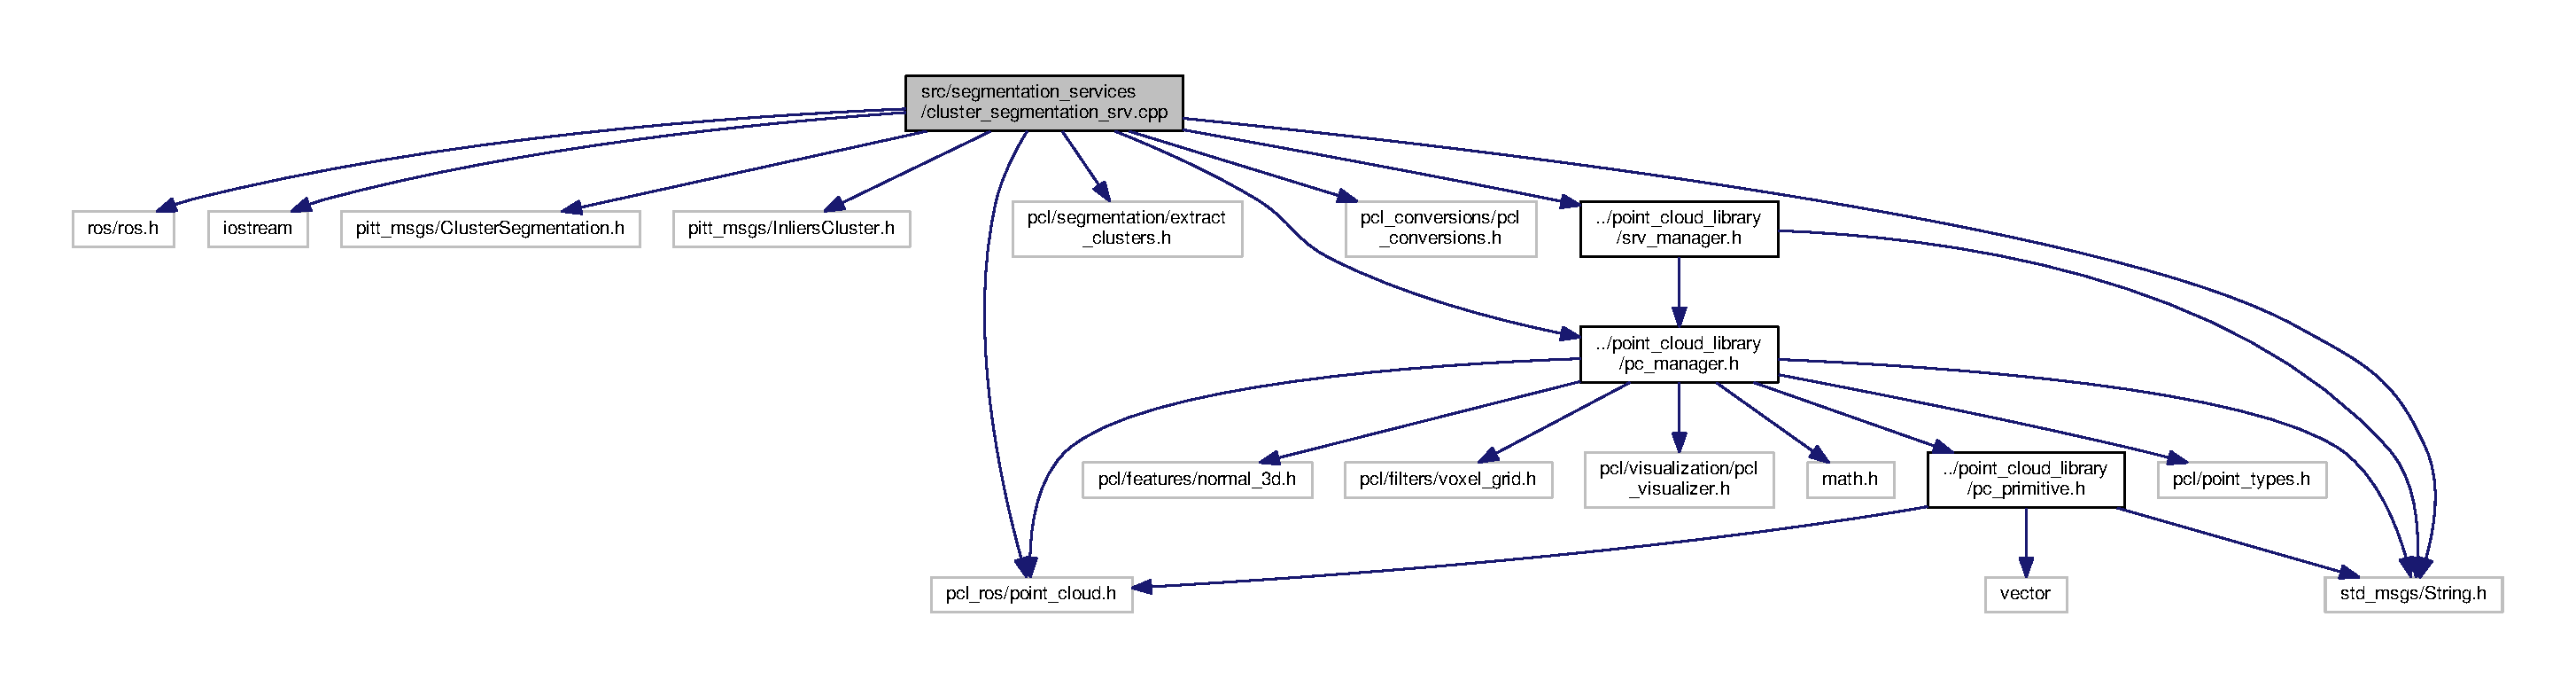
\includegraphics[width=350pt]{cluster__segmentation__srv_8cpp__incl}
\end{center}
\end{figure}
\subsection*{Functions}
\begin{DoxyCompactItemize}
\item 
bool \hyperlink{cluster__segmentation__srv_8cpp_ab4a01859dbef47b81c5744d85d81a097}{clusterize} (Cluster\-Segmentation\-::\-Request \&req, Cluster\-Segmentation\-::\-Response \&res)
\item 
int \hyperlink{cluster__segmentation__srv_8cpp_a3c04138a5bfe5d72780bb7e82a18e627}{main} (int argc, char $\ast$$\ast$argv)
\end{DoxyCompactItemize}
\subsection*{Variables}
\begin{DoxyCompactItemize}
\item 
ros\-::\-Node\-Handle $\ast$ \hyperlink{cluster__segmentation__srv_8cpp_afe3fec681d3658d114dfa8cfff163e82}{nh\-\_\-ptr} = N\-U\-L\-L
\item 
const double \hyperlink{cluster__segmentation__srv_8cpp_ac3266207fd4ea22474675128faa0f4b8}{C\-L\-U\-S\-T\-E\-R\-\_\-\-T\-O\-L\-E\-R\-A\-N\-C\-E\-\_\-\-D\-E\-F\-A\-U\-L\-T} = 0.\-03
\item 
const double \hyperlink{cluster__segmentation__srv_8cpp_a4a514e6543a3304047ee344acf96b565}{C\-L\-U\-S\-T\-E\-R\-\_\-\-M\-I\-N\-\_\-\-R\-A\-T\-E\-\_\-\-D\-E\-F\-A\-U\-L\-T} = 0.\-01
\item 
const double \hyperlink{cluster__segmentation__srv_8cpp_a65385475920af255961eeefb2abb959a}{C\-L\-U\-S\-T\-E\-R\-\_\-\-M\-A\-X\-\_\-\-R\-A\-T\-E\-\_\-\-D\-E\-F\-A\-U\-L\-T} = 0.\-99
\item 
const int \hyperlink{cluster__segmentation__srv_8cpp_a9ebfbbca18470dcde3857728e18e1247}{C\-L\-U\-S\-T\-E\-R\-\_\-\-M\-I\-N\-\_\-\-I\-N\-P\-U\-T\-\_\-\-S\-I\-Z\-E\-\_\-\-D\-E\-F\-A\-U\-L\-T} = 30
\end{DoxyCompactItemize}


\subsection{Function Documentation}
\hypertarget{cluster__segmentation__srv_8cpp_ab4a01859dbef47b81c5744d85d81a097}{\index{cluster\-\_\-segmentation\-\_\-srv.\-cpp@{cluster\-\_\-segmentation\-\_\-srv.\-cpp}!clusterize@{clusterize}}
\index{clusterize@{clusterize}!cluster_segmentation_srv.cpp@{cluster\-\_\-segmentation\-\_\-srv.\-cpp}}
\subsubsection[{clusterize}]{\setlength{\rightskip}{0pt plus 5cm}bool clusterize (
\begin{DoxyParamCaption}
\item[{Cluster\-Segmentation\-::\-Request \&}]{req, }
\item[{Cluster\-Segmentation\-::\-Response \&}]{res}
\end{DoxyParamCaption}
)}}\label{cluster__segmentation__srv_8cpp_ab4a01859dbef47b81c5744d85d81a097}


Definition at line 38 of file cluster\-\_\-segmentation\-\_\-srv.\-cpp.



References pcm\-::\-P\-C\-Manager\-::cloud\-For\-Ros\-Msg(), C\-L\-U\-S\-T\-E\-R\-\_\-\-M\-A\-X\-\_\-\-R\-A\-T\-E\-\_\-\-D\-E\-F\-A\-U\-L\-T, C\-L\-U\-S\-T\-E\-R\-\_\-\-M\-I\-N\-\_\-\-I\-N\-P\-U\-T\-\_\-\-S\-I\-Z\-E\-\_\-\-D\-E\-F\-A\-U\-L\-T, C\-L\-U\-S\-T\-E\-R\-\_\-\-M\-I\-N\-\_\-\-R\-A\-T\-E\-\_\-\-D\-E\-F\-A\-U\-L\-T, C\-L\-U\-S\-T\-E\-R\-\_\-\-T\-O\-L\-E\-R\-A\-N\-C\-E\-\_\-\-D\-E\-F\-A\-U\-L\-T, nh\-\_\-ptr, srvm\-::\-P\-A\-R\-A\-M\-\_\-\-N\-A\-M\-E\-\_\-\-C\-L\-U\-S\-T\-E\-R\-\_\-\-M\-A\-X\-\_\-\-R\-A\-T\-E, srvm\-::\-P\-A\-R\-A\-M\-\_\-\-N\-A\-M\-E\-\_\-\-C\-L\-U\-S\-T\-E\-R\-\_\-\-M\-I\-N\-\_\-\-R\-A\-T\-E, srvm\-::\-P\-A\-R\-A\-M\-\_\-\-N\-A\-M\-E\-\_\-\-C\-L\-U\-S\-T\-E\-R\-\_\-\-T\-O\-L\-E\-R\-A\-N\-C\-E, and pcm\-::tree().



Referenced by main().



Here is the call graph for this function\-:\nopagebreak
\begin{figure}[H]
\begin{center}
\leavevmode
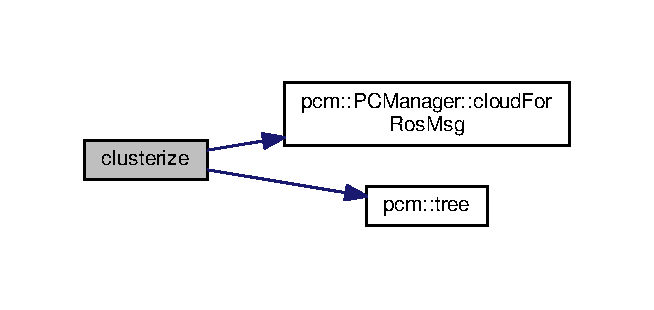
\includegraphics[width=314pt]{cluster__segmentation__srv_8cpp_ab4a01859dbef47b81c5744d85d81a097_cgraph}
\end{center}
\end{figure}


\hypertarget{cluster__segmentation__srv_8cpp_a3c04138a5bfe5d72780bb7e82a18e627}{\index{cluster\-\_\-segmentation\-\_\-srv.\-cpp@{cluster\-\_\-segmentation\-\_\-srv.\-cpp}!main@{main}}
\index{main@{main}!cluster_segmentation_srv.cpp@{cluster\-\_\-segmentation\-\_\-srv.\-cpp}}
\subsubsection[{main}]{\setlength{\rightskip}{0pt plus 5cm}int main (
\begin{DoxyParamCaption}
\item[{int}]{argc, }
\item[{char $\ast$$\ast$}]{argv}
\end{DoxyParamCaption}
)}}\label{cluster__segmentation__srv_8cpp_a3c04138a5bfe5d72780bb7e82a18e627}


Definition at line 118 of file cluster\-\_\-segmentation\-\_\-srv.\-cpp.



References clusterize(), nh\-\_\-ptr, and srvm\-::\-S\-R\-V\-\_\-\-N\-A\-M\-E\-\_\-\-C\-U\-S\-T\-E\-R\-\_\-\-F\-I\-L\-T\-E\-R.



Here is the call graph for this function\-:\nopagebreak
\begin{figure}[H]
\begin{center}
\leavevmode
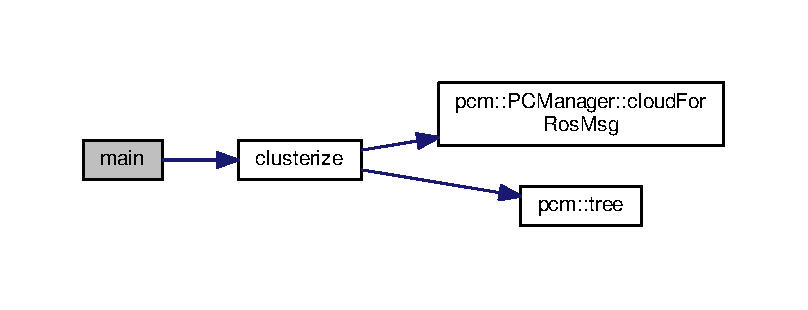
\includegraphics[width=350pt]{cluster__segmentation__srv_8cpp_a3c04138a5bfe5d72780bb7e82a18e627_cgraph}
\end{center}
\end{figure}




\subsection{Variable Documentation}
\hypertarget{cluster__segmentation__srv_8cpp_a65385475920af255961eeefb2abb959a}{\index{cluster\-\_\-segmentation\-\_\-srv.\-cpp@{cluster\-\_\-segmentation\-\_\-srv.\-cpp}!C\-L\-U\-S\-T\-E\-R\-\_\-\-M\-A\-X\-\_\-\-R\-A\-T\-E\-\_\-\-D\-E\-F\-A\-U\-L\-T@{C\-L\-U\-S\-T\-E\-R\-\_\-\-M\-A\-X\-\_\-\-R\-A\-T\-E\-\_\-\-D\-E\-F\-A\-U\-L\-T}}
\index{C\-L\-U\-S\-T\-E\-R\-\_\-\-M\-A\-X\-\_\-\-R\-A\-T\-E\-\_\-\-D\-E\-F\-A\-U\-L\-T@{C\-L\-U\-S\-T\-E\-R\-\_\-\-M\-A\-X\-\_\-\-R\-A\-T\-E\-\_\-\-D\-E\-F\-A\-U\-L\-T}!cluster_segmentation_srv.cpp@{cluster\-\_\-segmentation\-\_\-srv.\-cpp}}
\subsubsection[{C\-L\-U\-S\-T\-E\-R\-\_\-\-M\-A\-X\-\_\-\-R\-A\-T\-E\-\_\-\-D\-E\-F\-A\-U\-L\-T}]{\setlength{\rightskip}{0pt plus 5cm}const double C\-L\-U\-S\-T\-E\-R\-\_\-\-M\-A\-X\-\_\-\-R\-A\-T\-E\-\_\-\-D\-E\-F\-A\-U\-L\-T = 0.\-99}}\label{cluster__segmentation__srv_8cpp_a65385475920af255961eeefb2abb959a}


Definition at line 34 of file cluster\-\_\-segmentation\-\_\-srv.\-cpp.



Referenced by clusterize().

\hypertarget{cluster__segmentation__srv_8cpp_a9ebfbbca18470dcde3857728e18e1247}{\index{cluster\-\_\-segmentation\-\_\-srv.\-cpp@{cluster\-\_\-segmentation\-\_\-srv.\-cpp}!C\-L\-U\-S\-T\-E\-R\-\_\-\-M\-I\-N\-\_\-\-I\-N\-P\-U\-T\-\_\-\-S\-I\-Z\-E\-\_\-\-D\-E\-F\-A\-U\-L\-T@{C\-L\-U\-S\-T\-E\-R\-\_\-\-M\-I\-N\-\_\-\-I\-N\-P\-U\-T\-\_\-\-S\-I\-Z\-E\-\_\-\-D\-E\-F\-A\-U\-L\-T}}
\index{C\-L\-U\-S\-T\-E\-R\-\_\-\-M\-I\-N\-\_\-\-I\-N\-P\-U\-T\-\_\-\-S\-I\-Z\-E\-\_\-\-D\-E\-F\-A\-U\-L\-T@{C\-L\-U\-S\-T\-E\-R\-\_\-\-M\-I\-N\-\_\-\-I\-N\-P\-U\-T\-\_\-\-S\-I\-Z\-E\-\_\-\-D\-E\-F\-A\-U\-L\-T}!cluster_segmentation_srv.cpp@{cluster\-\_\-segmentation\-\_\-srv.\-cpp}}
\subsubsection[{C\-L\-U\-S\-T\-E\-R\-\_\-\-M\-I\-N\-\_\-\-I\-N\-P\-U\-T\-\_\-\-S\-I\-Z\-E\-\_\-\-D\-E\-F\-A\-U\-L\-T}]{\setlength{\rightskip}{0pt plus 5cm}const int C\-L\-U\-S\-T\-E\-R\-\_\-\-M\-I\-N\-\_\-\-I\-N\-P\-U\-T\-\_\-\-S\-I\-Z\-E\-\_\-\-D\-E\-F\-A\-U\-L\-T = 30}}\label{cluster__segmentation__srv_8cpp_a9ebfbbca18470dcde3857728e18e1247}


Definition at line 35 of file cluster\-\_\-segmentation\-\_\-srv.\-cpp.



Referenced by clusterize().

\hypertarget{cluster__segmentation__srv_8cpp_a4a514e6543a3304047ee344acf96b565}{\index{cluster\-\_\-segmentation\-\_\-srv.\-cpp@{cluster\-\_\-segmentation\-\_\-srv.\-cpp}!C\-L\-U\-S\-T\-E\-R\-\_\-\-M\-I\-N\-\_\-\-R\-A\-T\-E\-\_\-\-D\-E\-F\-A\-U\-L\-T@{C\-L\-U\-S\-T\-E\-R\-\_\-\-M\-I\-N\-\_\-\-R\-A\-T\-E\-\_\-\-D\-E\-F\-A\-U\-L\-T}}
\index{C\-L\-U\-S\-T\-E\-R\-\_\-\-M\-I\-N\-\_\-\-R\-A\-T\-E\-\_\-\-D\-E\-F\-A\-U\-L\-T@{C\-L\-U\-S\-T\-E\-R\-\_\-\-M\-I\-N\-\_\-\-R\-A\-T\-E\-\_\-\-D\-E\-F\-A\-U\-L\-T}!cluster_segmentation_srv.cpp@{cluster\-\_\-segmentation\-\_\-srv.\-cpp}}
\subsubsection[{C\-L\-U\-S\-T\-E\-R\-\_\-\-M\-I\-N\-\_\-\-R\-A\-T\-E\-\_\-\-D\-E\-F\-A\-U\-L\-T}]{\setlength{\rightskip}{0pt plus 5cm}const double C\-L\-U\-S\-T\-E\-R\-\_\-\-M\-I\-N\-\_\-\-R\-A\-T\-E\-\_\-\-D\-E\-F\-A\-U\-L\-T = 0.\-01}}\label{cluster__segmentation__srv_8cpp_a4a514e6543a3304047ee344acf96b565}


Definition at line 33 of file cluster\-\_\-segmentation\-\_\-srv.\-cpp.



Referenced by clusterize().

\hypertarget{cluster__segmentation__srv_8cpp_ac3266207fd4ea22474675128faa0f4b8}{\index{cluster\-\_\-segmentation\-\_\-srv.\-cpp@{cluster\-\_\-segmentation\-\_\-srv.\-cpp}!C\-L\-U\-S\-T\-E\-R\-\_\-\-T\-O\-L\-E\-R\-A\-N\-C\-E\-\_\-\-D\-E\-F\-A\-U\-L\-T@{C\-L\-U\-S\-T\-E\-R\-\_\-\-T\-O\-L\-E\-R\-A\-N\-C\-E\-\_\-\-D\-E\-F\-A\-U\-L\-T}}
\index{C\-L\-U\-S\-T\-E\-R\-\_\-\-T\-O\-L\-E\-R\-A\-N\-C\-E\-\_\-\-D\-E\-F\-A\-U\-L\-T@{C\-L\-U\-S\-T\-E\-R\-\_\-\-T\-O\-L\-E\-R\-A\-N\-C\-E\-\_\-\-D\-E\-F\-A\-U\-L\-T}!cluster_segmentation_srv.cpp@{cluster\-\_\-segmentation\-\_\-srv.\-cpp}}
\subsubsection[{C\-L\-U\-S\-T\-E\-R\-\_\-\-T\-O\-L\-E\-R\-A\-N\-C\-E\-\_\-\-D\-E\-F\-A\-U\-L\-T}]{\setlength{\rightskip}{0pt plus 5cm}const double C\-L\-U\-S\-T\-E\-R\-\_\-\-T\-O\-L\-E\-R\-A\-N\-C\-E\-\_\-\-D\-E\-F\-A\-U\-L\-T = 0.\-03}}\label{cluster__segmentation__srv_8cpp_ac3266207fd4ea22474675128faa0f4b8}


Definition at line 32 of file cluster\-\_\-segmentation\-\_\-srv.\-cpp.



Referenced by clusterize().

\hypertarget{cluster__segmentation__srv_8cpp_afe3fec681d3658d114dfa8cfff163e82}{\index{cluster\-\_\-segmentation\-\_\-srv.\-cpp@{cluster\-\_\-segmentation\-\_\-srv.\-cpp}!nh\-\_\-ptr@{nh\-\_\-ptr}}
\index{nh\-\_\-ptr@{nh\-\_\-ptr}!cluster_segmentation_srv.cpp@{cluster\-\_\-segmentation\-\_\-srv.\-cpp}}
\subsubsection[{nh\-\_\-ptr}]{\setlength{\rightskip}{0pt plus 5cm}ros\-::\-Node\-Handle$\ast$ nh\-\_\-ptr = N\-U\-L\-L}}\label{cluster__segmentation__srv_8cpp_afe3fec681d3658d114dfa8cfff163e82}


Definition at line 29 of file cluster\-\_\-segmentation\-\_\-srv.\-cpp.



Referenced by clusterize(), and main().


\hypertarget{cone__segmentation__srv_8cpp}{\section{src/segmentation\-\_\-services/cone\-\_\-segmentation\-\_\-srv.cpp File Reference}
\label{cone__segmentation__srv_8cpp}\index{src/segmentation\-\_\-services/cone\-\_\-segmentation\-\_\-srv.\-cpp@{src/segmentation\-\_\-services/cone\-\_\-segmentation\-\_\-srv.\-cpp}}
}
{\ttfamily \#include \char`\"{}ros/ros.\-h\char`\"{}}\\*
{\ttfamily \#include $<$pcl\-\_\-ros/point\-\_\-cloud.\-h$>$}\\*
{\ttfamily \#include $<$pcl/segmentation/sac\-\_\-segmentation.\-h$>$}\\*
{\ttfamily \#include \char`\"{}pitt\-\_\-msgs/\-Primitive\-Segmentation.\-h\char`\"{}}\\*
{\ttfamily \#include \char`\"{}../point\-\_\-cloud\-\_\-library/pc\-\_\-manager.\-h\char`\"{}}\\*
{\ttfamily \#include \char`\"{}../point\-\_\-cloud\-\_\-library/srv\-\_\-manager.\-h\char`\"{}}\\*
{\ttfamily \#include $<$boost/thread.\-hpp$>$}\\*
{\ttfamily \#include $<$boost/thread/mutex.\-hpp$>$}\\*
{\ttfamily \#include $<$boost/format.\-hpp$>$}\\*
Include dependency graph for cone\-\_\-segmentation\-\_\-srv.\-cpp\-:
\nopagebreak
\begin{figure}[H]
\begin{center}
\leavevmode
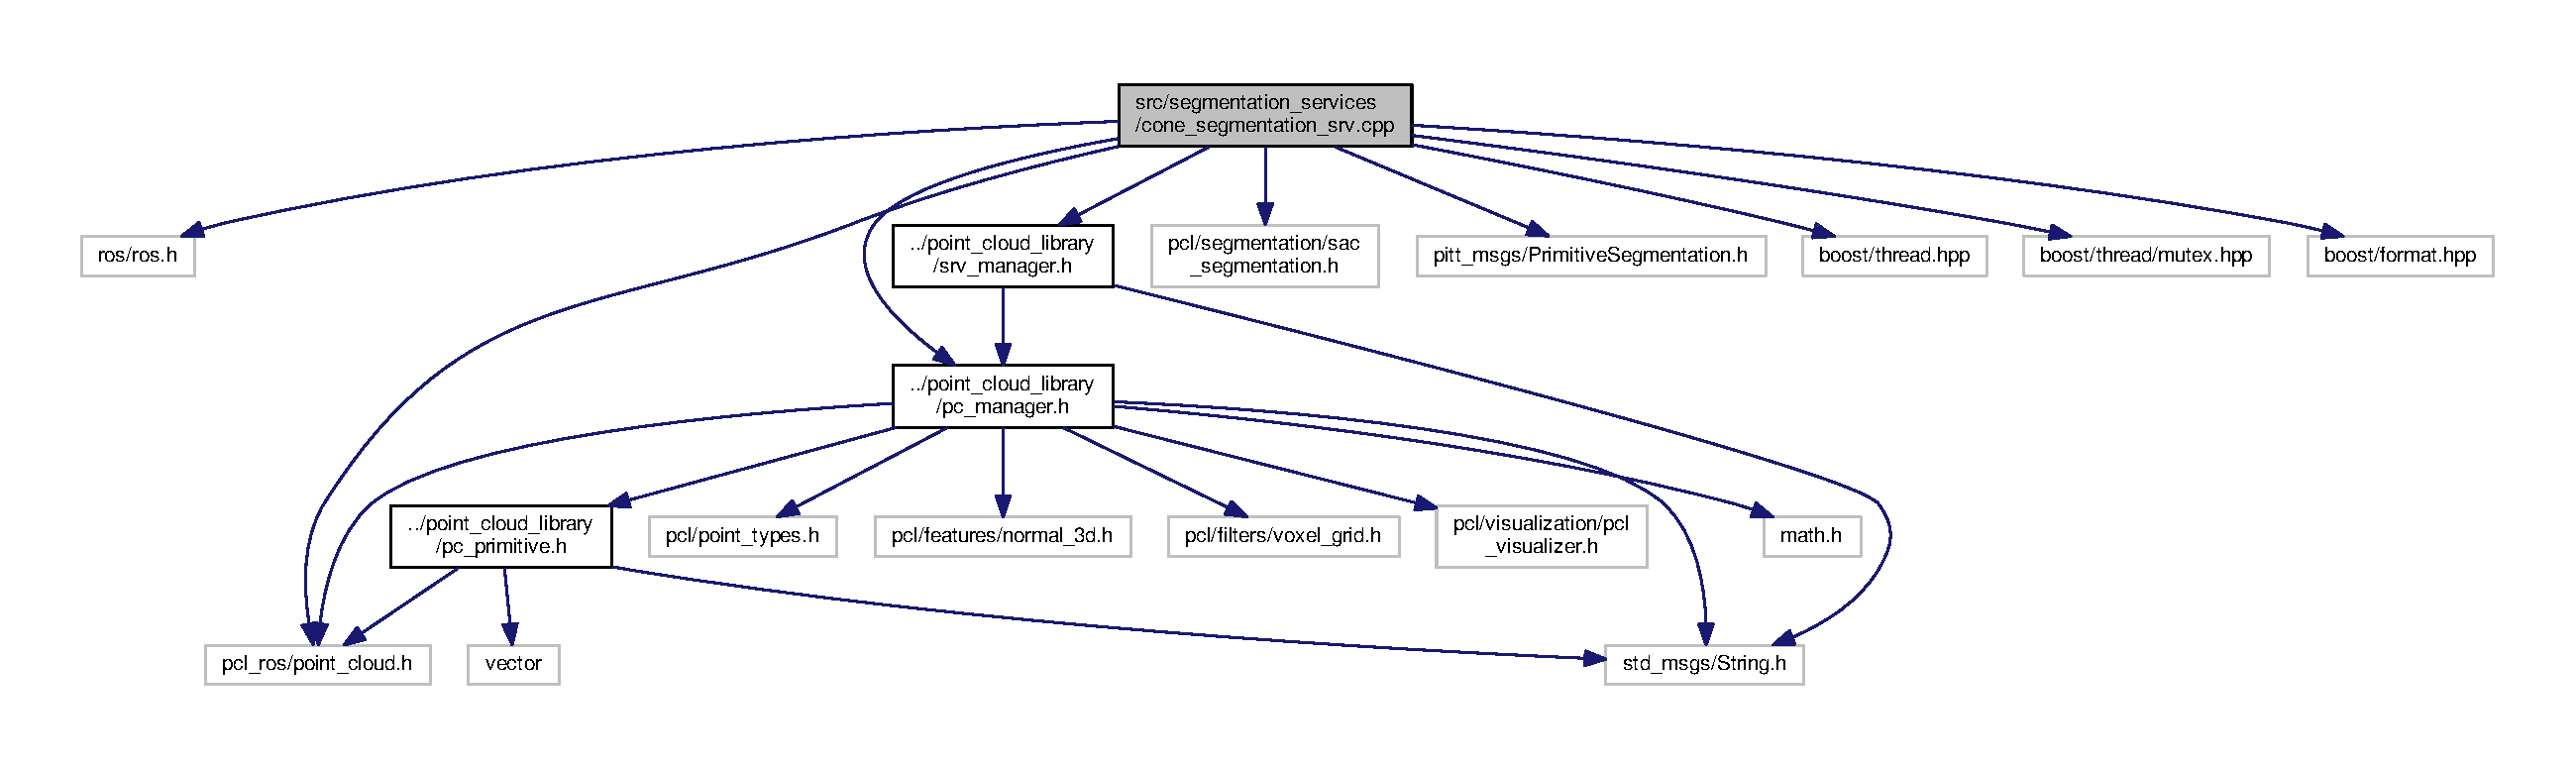
\includegraphics[width=350pt]{cone__segmentation__srv_8cpp__incl}
\end{center}
\end{figure}
\subsection*{Classes}
\begin{DoxyCompactItemize}
\item 
struct \hyperlink{structvector3d}{vector3d}
\end{DoxyCompactItemize}
\subsection*{Functions}
\begin{DoxyCompactItemize}
\item 
void \hyperlink{cone__segmentation__srv_8cpp_aca73ab26cae45b4b998a3cca9e4f75bc}{vis\-Spin} ()
\item 
\hyperlink{structvector3d}{vector3d} \hyperlink{cone__segmentation__srv_8cpp_a18fcf7fa2e84ef1176c2ca1abed744cf}{get\-Normalize\-Axes\-Direction\-Vector} (Model\-Coefficients\-::\-Ptr coefficients)
\item 
\hyperlink{structvector3d}{vector3d} \hyperlink{cone__segmentation__srv_8cpp_a255909b8e4ba570eea6756718bf79df1}{get\-Point\-On\-Axes} (Model\-Coefficients\-::\-Ptr coefficients, \hyperlink{structvector3d}{vector3d} direction, float t)
\item 
\hyperlink{structvector3d}{vector3d} \hyperlink{cone__segmentation__srv_8cpp_a00c9eb33d55847838be7bf32c23d1893}{get\-Vector\-Between\-Points} (\hyperlink{structvector3d}{vector3d} p1, \hyperlink{structvector3d}{vector3d} p2)
\item 
bool \hyperlink{cone__segmentation__srv_8cpp_a546c9eceb49309d94085dada4aae1755}{ransac\-Cone\-Detaction} (Primitive\-Segmentation\-::\-Request \&req, Primitive\-Segmentation\-::\-Response \&res)
\item 
int \hyperlink{cone__segmentation__srv_8cpp_a3c04138a5bfe5d72780bb7e82a18e627}{main} (int argc, char $\ast$$\ast$argv)
\end{DoxyCompactItemize}
\subsection*{Variables}
\begin{DoxyCompactItemize}
\item 
ros\-::\-Node\-Handle $\ast$ \hyperlink{cone__segmentation__srv_8cpp_afe3fec681d3658d114dfa8cfff163e82}{nh\-\_\-ptr} = N\-U\-L\-L
\item 
static const double \hyperlink{cone__segmentation__srv_8cpp_a58313fd9217054625ac4527d3633193e}{C\-O\-N\-E\-\_\-\-N\-O\-R\-M\-A\-L\-\_\-\-D\-I\-S\-T\-A\-N\-C\-E\-\_\-\-W\-E\-I\-G\-T\-H} = 0.\-0006
\item 
static const double \hyperlink{cone__segmentation__srv_8cpp_a8fe7696768fcf8c3d5659116abacee6f}{C\-O\-N\-E\-\_\-\-D\-I\-S\-T\-A\-N\-C\-E\-\_\-\-T\-H} = 0.\-0055
\item 
static const double \hyperlink{cone__segmentation__srv_8cpp_a9080b5047d249f3d1b9ba3581c77521f}{C\-O\-N\-E\-\_\-\-M\-I\-N\-\_\-\-R\-A\-D\-I\-U\-S\-\_\-\-L\-I\-M\-I\-T} = 0.\-001
\item 
static const double \hyperlink{cone__segmentation__srv_8cpp_a384e57e531632b1d04ae3174520b5063}{C\-O\-N\-E\-\_\-\-M\-A\-X\-\_\-\-R\-A\-D\-I\-U\-S\-\_\-\-L\-I\-M\-I\-T} = 0.\-500
\item 
static const int \hyperlink{cone__segmentation__srv_8cpp_af6c0c21521af2937dffda5d2ecf87cf5}{C\-O\-N\-E\-\_\-\-M\-A\-X\-\_\-\-I\-T\-E\-R\-A\-T\-I\-O\-N\-\_\-\-L\-I\-M\-I\-T} = 1000
\item 
static const double \hyperlink{cone__segmentation__srv_8cpp_ade9321247b9be50dd895dc3edb7559f3}{C\-O\-N\-E\-\_\-\-E\-P\-S\-\_\-\-A\-N\-G\-L\-E\-\_\-\-T\-H} = 0.\-4
\item 
static const double \hyperlink{cone__segmentation__srv_8cpp_a3e7e19175ddd4f8f95f350c1b86fd5c7}{C\-O\-N\-E\-\_\-\-M\-I\-N\-\_\-\-O\-P\-E\-N\-I\-N\-G\-\_\-\-A\-N\-G\-L\-E\-\_\-\-D\-E\-G\-R\-E\-E} = 10.\-0
\item 
static const double \hyperlink{cone__segmentation__srv_8cpp_a1856e890b10fc7ece03e7cee6472f601}{C\-O\-N\-E\-\_\-\-M\-A\-X\-\_\-\-O\-P\-E\-N\-I\-N\-G\-\_\-\-A\-N\-G\-L\-E\-\_\-\-D\-E\-G\-R\-E\-E} = 170.\-0
\item 
const bool \hyperlink{cone__segmentation__srv_8cpp_a20f88026cd9df482d817a3868c20fe43}{V\-I\-S\-U\-A\-L\-I\-Z\-E\-\_\-\-R\-E\-S\-U\-L\-T} = false
\item 
boost\-::shared\-\_\-ptr\\*
$<$ \hyperlink{pc__manager_8h_a38c805dbc7ad6f06109b85c8e540817a}{visualization\-::\-P\-C\-L\-Visualizer} $>$ \hyperlink{cone__segmentation__srv_8cpp_a6c2d87234fca8dcca11f888098558986}{vis}
\item 
boost\-::thread \hyperlink{cone__segmentation__srv_8cpp_ab83e6219895a4d26706c0d858f8ec288}{vis\-\_\-thread}
\item 
boost\-::mutex \hyperlink{cone__segmentation__srv_8cpp_a0dc8882293908d9c8cc15f76a2a49588}{vis\-\_\-mutex}
\end{DoxyCompactItemize}


\subsection{Function Documentation}
\hypertarget{cone__segmentation__srv_8cpp_a18fcf7fa2e84ef1176c2ca1abed744cf}{\index{cone\-\_\-segmentation\-\_\-srv.\-cpp@{cone\-\_\-segmentation\-\_\-srv.\-cpp}!get\-Normalize\-Axes\-Direction\-Vector@{get\-Normalize\-Axes\-Direction\-Vector}}
\index{get\-Normalize\-Axes\-Direction\-Vector@{get\-Normalize\-Axes\-Direction\-Vector}!cone_segmentation_srv.cpp@{cone\-\_\-segmentation\-\_\-srv.\-cpp}}
\subsubsection[{get\-Normalize\-Axes\-Direction\-Vector}]{\setlength{\rightskip}{0pt plus 5cm}{\bf vector3d} get\-Normalize\-Axes\-Direction\-Vector (
\begin{DoxyParamCaption}
\item[{Model\-Coefficients\-::\-Ptr}]{coefficients}
\end{DoxyParamCaption}
)}}\label{cone__segmentation__srv_8cpp_a18fcf7fa2e84ef1176c2ca1abed744cf}


Definition at line 54 of file cone\-\_\-segmentation\-\_\-srv.\-cpp.



References vector3d\-::x, vector3d\-::y, and vector3d\-::z.



Referenced by ransac\-Cone\-Detaction().

\hypertarget{cone__segmentation__srv_8cpp_a255909b8e4ba570eea6756718bf79df1}{\index{cone\-\_\-segmentation\-\_\-srv.\-cpp@{cone\-\_\-segmentation\-\_\-srv.\-cpp}!get\-Point\-On\-Axes@{get\-Point\-On\-Axes}}
\index{get\-Point\-On\-Axes@{get\-Point\-On\-Axes}!cone_segmentation_srv.cpp@{cone\-\_\-segmentation\-\_\-srv.\-cpp}}
\subsubsection[{get\-Point\-On\-Axes}]{\setlength{\rightskip}{0pt plus 5cm}{\bf vector3d} get\-Point\-On\-Axes (
\begin{DoxyParamCaption}
\item[{Model\-Coefficients\-::\-Ptr}]{coefficients, }
\item[{{\bf vector3d}}]{direction, }
\item[{float}]{t}
\end{DoxyParamCaption}
)}}\label{cone__segmentation__srv_8cpp_a255909b8e4ba570eea6756718bf79df1}


Definition at line 65 of file cone\-\_\-segmentation\-\_\-srv.\-cpp.



References vector3d\-::x, vector3d\-::y, and vector3d\-::z.



Referenced by ransac\-Cone\-Detaction().

\hypertarget{cone__segmentation__srv_8cpp_a00c9eb33d55847838be7bf32c23d1893}{\index{cone\-\_\-segmentation\-\_\-srv.\-cpp@{cone\-\_\-segmentation\-\_\-srv.\-cpp}!get\-Vector\-Between\-Points@{get\-Vector\-Between\-Points}}
\index{get\-Vector\-Between\-Points@{get\-Vector\-Between\-Points}!cone_segmentation_srv.cpp@{cone\-\_\-segmentation\-\_\-srv.\-cpp}}
\subsubsection[{get\-Vector\-Between\-Points}]{\setlength{\rightskip}{0pt plus 5cm}{\bf vector3d} get\-Vector\-Between\-Points (
\begin{DoxyParamCaption}
\item[{{\bf vector3d}}]{p1, }
\item[{{\bf vector3d}}]{p2}
\end{DoxyParamCaption}
)}}\label{cone__segmentation__srv_8cpp_a00c9eb33d55847838be7bf32c23d1893}


Definition at line 74 of file cone\-\_\-segmentation\-\_\-srv.\-cpp.



References vector3d\-::x, vector3d\-::y, and vector3d\-::z.



Referenced by ransac\-Cone\-Detaction().

\hypertarget{cone__segmentation__srv_8cpp_a3c04138a5bfe5d72780bb7e82a18e627}{\index{cone\-\_\-segmentation\-\_\-srv.\-cpp@{cone\-\_\-segmentation\-\_\-srv.\-cpp}!main@{main}}
\index{main@{main}!cone_segmentation_srv.cpp@{cone\-\_\-segmentation\-\_\-srv.\-cpp}}
\subsubsection[{main}]{\setlength{\rightskip}{0pt plus 5cm}int main (
\begin{DoxyParamCaption}
\item[{int}]{argc, }
\item[{char $\ast$$\ast$}]{argv}
\end{DoxyParamCaption}
)}}\label{cone__segmentation__srv_8cpp_a3c04138a5bfe5d72780bb7e82a18e627}


Definition at line 220 of file cone\-\_\-segmentation\-\_\-srv.\-cpp.



References pcm\-::\-P\-C\-Manager\-::create\-Visor(), nh\-\_\-ptr, ransac\-Cone\-Detaction(), srvm\-::\-S\-R\-V\-\_\-\-N\-A\-M\-E\-\_\-\-R\-A\-N\-S\-A\-C\-\_\-\-C\-O\-N\-E\-\_\-\-F\-I\-L\-T\-E\-R, vis, vis\-\_\-thread, vis\-Spin(), and V\-I\-S\-U\-A\-L\-I\-Z\-E\-\_\-\-R\-E\-S\-U\-L\-T.



Here is the call graph for this function\-:
\nopagebreak
\begin{figure}[H]
\begin{center}
\leavevmode
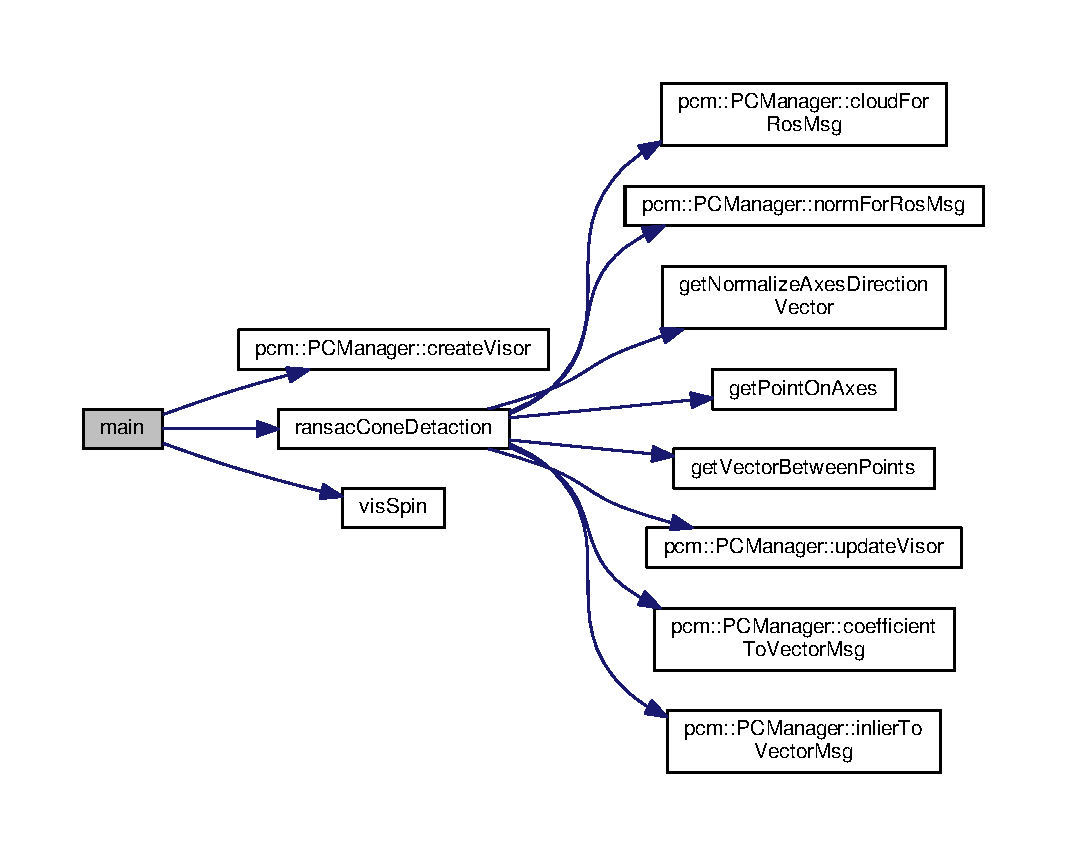
\includegraphics[width=350pt]{cone__segmentation__srv_8cpp_a3c04138a5bfe5d72780bb7e82a18e627_cgraph}
\end{center}
\end{figure}


\hypertarget{cone__segmentation__srv_8cpp_a546c9eceb49309d94085dada4aae1755}{\index{cone\-\_\-segmentation\-\_\-srv.\-cpp@{cone\-\_\-segmentation\-\_\-srv.\-cpp}!ransac\-Cone\-Detaction@{ransac\-Cone\-Detaction}}
\index{ransac\-Cone\-Detaction@{ransac\-Cone\-Detaction}!cone_segmentation_srv.cpp@{cone\-\_\-segmentation\-\_\-srv.\-cpp}}
\subsubsection[{ransac\-Cone\-Detaction}]{\setlength{\rightskip}{0pt plus 5cm}bool ransac\-Cone\-Detaction (
\begin{DoxyParamCaption}
\item[{Primitive\-Segmentation\-::\-Request \&}]{req, }
\item[{Primitive\-Segmentation\-::\-Response \&}]{res}
\end{DoxyParamCaption}
)}}\label{cone__segmentation__srv_8cpp_a546c9eceb49309d94085dada4aae1755}


Definition at line 83 of file cone\-\_\-segmentation\-\_\-srv.\-cpp.



References pcm\-::\-P\-C\-Manager\-::cloud\-For\-Ros\-Msg(), pcm\-::\-P\-C\-Manager\-::coefficient\-To\-Vector\-Msg(), C\-O\-N\-E\-\_\-\-D\-I\-S\-T\-A\-N\-C\-E\-\_\-\-T\-H, C\-O\-N\-E\-\_\-\-E\-P\-S\-\_\-\-A\-N\-G\-L\-E\-\_\-\-T\-H, C\-O\-N\-E\-\_\-\-M\-A\-X\-\_\-\-I\-T\-E\-R\-A\-T\-I\-O\-N\-\_\-\-L\-I\-M\-I\-T, C\-O\-N\-E\-\_\-\-M\-A\-X\-\_\-\-O\-P\-E\-N\-I\-N\-G\-\_\-\-A\-N\-G\-L\-E\-\_\-\-D\-E\-G\-R\-E\-E, C\-O\-N\-E\-\_\-\-M\-A\-X\-\_\-\-R\-A\-D\-I\-U\-S\-\_\-\-L\-I\-M\-I\-T, C\-O\-N\-E\-\_\-\-M\-I\-N\-\_\-\-O\-P\-E\-N\-I\-N\-G\-\_\-\-A\-N\-G\-L\-E\-\_\-\-D\-E\-G\-R\-E\-E, C\-O\-N\-E\-\_\-\-M\-I\-N\-\_\-\-R\-A\-D\-I\-U\-S\-\_\-\-L\-I\-M\-I\-T, C\-O\-N\-E\-\_\-\-N\-O\-R\-M\-A\-L\-\_\-\-D\-I\-S\-T\-A\-N\-C\-E\-\_\-\-W\-E\-I\-G\-T\-H, get\-Normalize\-Axes\-Direction\-Vector(), get\-Point\-On\-Axes(), get\-Vector\-Between\-Points(), pcm\-::\-P\-C\-Manager\-::inlier\-To\-Vector\-Msg(), nh\-\_\-ptr, pcm\-::\-P\-C\-Manager\-::norm\-For\-Ros\-Msg(), srvm\-::\-P\-A\-R\-A\-M\-\_\-\-N\-A\-M\-E\-\_\-\-C\-O\-N\-E\-\_\-\-D\-I\-S\-T\-A\-N\-C\-E\-\_\-\-T\-H, srvm\-::\-P\-A\-R\-A\-M\-\_\-\-N\-A\-M\-E\-\_\-\-C\-O\-N\-E\-\_\-\-E\-P\-S\-\_\-\-A\-N\-G\-L\-E\-\_\-\-T\-H, srvm\-::\-P\-A\-R\-A\-M\-\_\-\-N\-A\-M\-E\-\_\-\-C\-O\-N\-E\-\_\-\-M\-A\-X\-\_\-\-I\-T\-E\-R\-A\-T\-I\-O\-N\-\_\-\-L\-I\-M\-I\-T, srvm\-::\-P\-A\-R\-A\-M\-\_\-\-N\-A\-M\-E\-\_\-\-C\-O\-N\-E\-\_\-\-M\-A\-X\-\_\-\-O\-P\-E\-N\-I\-N\-G\-\_\-\-A\-N\-G\-L\-E\-\_\-\-D\-E\-G\-R\-E\-E, srvm\-::\-P\-A\-R\-A\-M\-\_\-\-N\-A\-M\-E\-\_\-\-C\-O\-N\-E\-\_\-\-M\-A\-X\-\_\-\-R\-A\-D\-I\-U\-S\-\_\-\-L\-I\-M\-I\-T, srvm\-::\-P\-A\-R\-A\-M\-\_\-\-N\-A\-M\-E\-\_\-\-C\-O\-N\-E\-\_\-\-M\-I\-N\-\_\-\-O\-P\-E\-N\-I\-N\-G\-\_\-\-A\-N\-G\-L\-E\-\_\-\-D\-E\-G\-R\-E\-E, srvm\-::\-P\-A\-R\-A\-M\-\_\-\-N\-A\-M\-E\-\_\-\-C\-O\-N\-E\-\_\-\-M\-I\-N\-\_\-\-R\-A\-D\-I\-U\-S\-\_\-\-L\-I\-M\-I\-T, srvm\-::\-P\-A\-R\-A\-M\-\_\-\-N\-A\-M\-E\-\_\-\-C\-O\-N\-E\-\_\-\-N\-O\-R\-M\-A\-L\-\_\-\-D\-I\-S\-T\-A\-N\-C\-E\-\_\-\-W\-E\-I\-G\-H\-T, seg, pcm\-::\-P\-C\-Manager\-::update\-Visor(), vis, vis\-\_\-mutex, V\-I\-S\-U\-A\-L\-I\-Z\-E\-\_\-\-R\-E\-S\-U\-L\-T, vector3d\-::x, vector3d\-::y, and vector3d\-::z.



Referenced by main().



Here is the call graph for this function\-:
\nopagebreak
\begin{figure}[H]
\begin{center}
\leavevmode
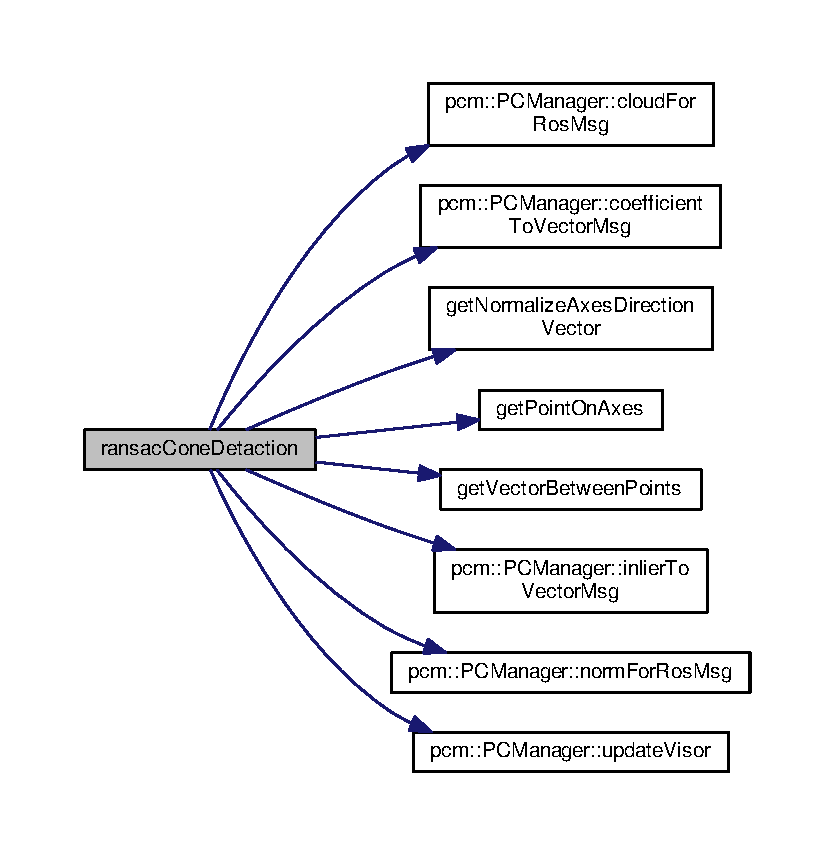
\includegraphics[width=350pt]{cone__segmentation__srv_8cpp_a546c9eceb49309d94085dada4aae1755_cgraph}
\end{center}
\end{figure}


\hypertarget{cone__segmentation__srv_8cpp_aca73ab26cae45b4b998a3cca9e4f75bc}{\index{cone\-\_\-segmentation\-\_\-srv.\-cpp@{cone\-\_\-segmentation\-\_\-srv.\-cpp}!vis\-Spin@{vis\-Spin}}
\index{vis\-Spin@{vis\-Spin}!cone_segmentation_srv.cpp@{cone\-\_\-segmentation\-\_\-srv.\-cpp}}
\subsubsection[{vis\-Spin}]{\setlength{\rightskip}{0pt plus 5cm}void vis\-Spin (
\begin{DoxyParamCaption}
{}
\end{DoxyParamCaption}
)}}\label{cone__segmentation__srv_8cpp_aca73ab26cae45b4b998a3cca9e4f75bc}


Definition at line 46 of file cone\-\_\-segmentation\-\_\-srv.\-cpp.



References vis, and vis\-\_\-mutex.



Referenced by main().



\subsection{Variable Documentation}
\hypertarget{cone__segmentation__srv_8cpp_a8fe7696768fcf8c3d5659116abacee6f}{\index{cone\-\_\-segmentation\-\_\-srv.\-cpp@{cone\-\_\-segmentation\-\_\-srv.\-cpp}!C\-O\-N\-E\-\_\-\-D\-I\-S\-T\-A\-N\-C\-E\-\_\-\-T\-H@{C\-O\-N\-E\-\_\-\-D\-I\-S\-T\-A\-N\-C\-E\-\_\-\-T\-H}}
\index{C\-O\-N\-E\-\_\-\-D\-I\-S\-T\-A\-N\-C\-E\-\_\-\-T\-H@{C\-O\-N\-E\-\_\-\-D\-I\-S\-T\-A\-N\-C\-E\-\_\-\-T\-H}!cone_segmentation_srv.cpp@{cone\-\_\-segmentation\-\_\-srv.\-cpp}}
\subsubsection[{C\-O\-N\-E\-\_\-\-D\-I\-S\-T\-A\-N\-C\-E\-\_\-\-T\-H}]{\setlength{\rightskip}{0pt plus 5cm}const double C\-O\-N\-E\-\_\-\-D\-I\-S\-T\-A\-N\-C\-E\-\_\-\-T\-H = 0.\-0055\hspace{0.3cm}{\ttfamily [static]}}}\label{cone__segmentation__srv_8cpp_a8fe7696768fcf8c3d5659116abacee6f}


Definition at line 25 of file cone\-\_\-segmentation\-\_\-srv.\-cpp.



Referenced by ransac\-Cone\-Detaction().

\hypertarget{cone__segmentation__srv_8cpp_ade9321247b9be50dd895dc3edb7559f3}{\index{cone\-\_\-segmentation\-\_\-srv.\-cpp@{cone\-\_\-segmentation\-\_\-srv.\-cpp}!C\-O\-N\-E\-\_\-\-E\-P\-S\-\_\-\-A\-N\-G\-L\-E\-\_\-\-T\-H@{C\-O\-N\-E\-\_\-\-E\-P\-S\-\_\-\-A\-N\-G\-L\-E\-\_\-\-T\-H}}
\index{C\-O\-N\-E\-\_\-\-E\-P\-S\-\_\-\-A\-N\-G\-L\-E\-\_\-\-T\-H@{C\-O\-N\-E\-\_\-\-E\-P\-S\-\_\-\-A\-N\-G\-L\-E\-\_\-\-T\-H}!cone_segmentation_srv.cpp@{cone\-\_\-segmentation\-\_\-srv.\-cpp}}
\subsubsection[{C\-O\-N\-E\-\_\-\-E\-P\-S\-\_\-\-A\-N\-G\-L\-E\-\_\-\-T\-H}]{\setlength{\rightskip}{0pt plus 5cm}const double C\-O\-N\-E\-\_\-\-E\-P\-S\-\_\-\-A\-N\-G\-L\-E\-\_\-\-T\-H = 0.\-4\hspace{0.3cm}{\ttfamily [static]}}}\label{cone__segmentation__srv_8cpp_ade9321247b9be50dd895dc3edb7559f3}


Definition at line 29 of file cone\-\_\-segmentation\-\_\-srv.\-cpp.



Referenced by ransac\-Cone\-Detaction().

\hypertarget{cone__segmentation__srv_8cpp_af6c0c21521af2937dffda5d2ecf87cf5}{\index{cone\-\_\-segmentation\-\_\-srv.\-cpp@{cone\-\_\-segmentation\-\_\-srv.\-cpp}!C\-O\-N\-E\-\_\-\-M\-A\-X\-\_\-\-I\-T\-E\-R\-A\-T\-I\-O\-N\-\_\-\-L\-I\-M\-I\-T@{C\-O\-N\-E\-\_\-\-M\-A\-X\-\_\-\-I\-T\-E\-R\-A\-T\-I\-O\-N\-\_\-\-L\-I\-M\-I\-T}}
\index{C\-O\-N\-E\-\_\-\-M\-A\-X\-\_\-\-I\-T\-E\-R\-A\-T\-I\-O\-N\-\_\-\-L\-I\-M\-I\-T@{C\-O\-N\-E\-\_\-\-M\-A\-X\-\_\-\-I\-T\-E\-R\-A\-T\-I\-O\-N\-\_\-\-L\-I\-M\-I\-T}!cone_segmentation_srv.cpp@{cone\-\_\-segmentation\-\_\-srv.\-cpp}}
\subsubsection[{C\-O\-N\-E\-\_\-\-M\-A\-X\-\_\-\-I\-T\-E\-R\-A\-T\-I\-O\-N\-\_\-\-L\-I\-M\-I\-T}]{\setlength{\rightskip}{0pt plus 5cm}const int C\-O\-N\-E\-\_\-\-M\-A\-X\-\_\-\-I\-T\-E\-R\-A\-T\-I\-O\-N\-\_\-\-L\-I\-M\-I\-T = 1000\hspace{0.3cm}{\ttfamily [static]}}}\label{cone__segmentation__srv_8cpp_af6c0c21521af2937dffda5d2ecf87cf5}


Definition at line 28 of file cone\-\_\-segmentation\-\_\-srv.\-cpp.



Referenced by ransac\-Cone\-Detaction().

\hypertarget{cone__segmentation__srv_8cpp_a1856e890b10fc7ece03e7cee6472f601}{\index{cone\-\_\-segmentation\-\_\-srv.\-cpp@{cone\-\_\-segmentation\-\_\-srv.\-cpp}!C\-O\-N\-E\-\_\-\-M\-A\-X\-\_\-\-O\-P\-E\-N\-I\-N\-G\-\_\-\-A\-N\-G\-L\-E\-\_\-\-D\-E\-G\-R\-E\-E@{C\-O\-N\-E\-\_\-\-M\-A\-X\-\_\-\-O\-P\-E\-N\-I\-N\-G\-\_\-\-A\-N\-G\-L\-E\-\_\-\-D\-E\-G\-R\-E\-E}}
\index{C\-O\-N\-E\-\_\-\-M\-A\-X\-\_\-\-O\-P\-E\-N\-I\-N\-G\-\_\-\-A\-N\-G\-L\-E\-\_\-\-D\-E\-G\-R\-E\-E@{C\-O\-N\-E\-\_\-\-M\-A\-X\-\_\-\-O\-P\-E\-N\-I\-N\-G\-\_\-\-A\-N\-G\-L\-E\-\_\-\-D\-E\-G\-R\-E\-E}!cone_segmentation_srv.cpp@{cone\-\_\-segmentation\-\_\-srv.\-cpp}}
\subsubsection[{C\-O\-N\-E\-\_\-\-M\-A\-X\-\_\-\-O\-P\-E\-N\-I\-N\-G\-\_\-\-A\-N\-G\-L\-E\-\_\-\-D\-E\-G\-R\-E\-E}]{\setlength{\rightskip}{0pt plus 5cm}const double C\-O\-N\-E\-\_\-\-M\-A\-X\-\_\-\-O\-P\-E\-N\-I\-N\-G\-\_\-\-A\-N\-G\-L\-E\-\_\-\-D\-E\-G\-R\-E\-E = 170.\-0\hspace{0.3cm}{\ttfamily [static]}}}\label{cone__segmentation__srv_8cpp_a1856e890b10fc7ece03e7cee6472f601}


Definition at line 31 of file cone\-\_\-segmentation\-\_\-srv.\-cpp.



Referenced by ransac\-Cone\-Detaction().

\hypertarget{cone__segmentation__srv_8cpp_a384e57e531632b1d04ae3174520b5063}{\index{cone\-\_\-segmentation\-\_\-srv.\-cpp@{cone\-\_\-segmentation\-\_\-srv.\-cpp}!C\-O\-N\-E\-\_\-\-M\-A\-X\-\_\-\-R\-A\-D\-I\-U\-S\-\_\-\-L\-I\-M\-I\-T@{C\-O\-N\-E\-\_\-\-M\-A\-X\-\_\-\-R\-A\-D\-I\-U\-S\-\_\-\-L\-I\-M\-I\-T}}
\index{C\-O\-N\-E\-\_\-\-M\-A\-X\-\_\-\-R\-A\-D\-I\-U\-S\-\_\-\-L\-I\-M\-I\-T@{C\-O\-N\-E\-\_\-\-M\-A\-X\-\_\-\-R\-A\-D\-I\-U\-S\-\_\-\-L\-I\-M\-I\-T}!cone_segmentation_srv.cpp@{cone\-\_\-segmentation\-\_\-srv.\-cpp}}
\subsubsection[{C\-O\-N\-E\-\_\-\-M\-A\-X\-\_\-\-R\-A\-D\-I\-U\-S\-\_\-\-L\-I\-M\-I\-T}]{\setlength{\rightskip}{0pt plus 5cm}const double C\-O\-N\-E\-\_\-\-M\-A\-X\-\_\-\-R\-A\-D\-I\-U\-S\-\_\-\-L\-I\-M\-I\-T = 0.\-500\hspace{0.3cm}{\ttfamily [static]}}}\label{cone__segmentation__srv_8cpp_a384e57e531632b1d04ae3174520b5063}


Definition at line 27 of file cone\-\_\-segmentation\-\_\-srv.\-cpp.



Referenced by ransac\-Cone\-Detaction().

\hypertarget{cone__segmentation__srv_8cpp_a3e7e19175ddd4f8f95f350c1b86fd5c7}{\index{cone\-\_\-segmentation\-\_\-srv.\-cpp@{cone\-\_\-segmentation\-\_\-srv.\-cpp}!C\-O\-N\-E\-\_\-\-M\-I\-N\-\_\-\-O\-P\-E\-N\-I\-N\-G\-\_\-\-A\-N\-G\-L\-E\-\_\-\-D\-E\-G\-R\-E\-E@{C\-O\-N\-E\-\_\-\-M\-I\-N\-\_\-\-O\-P\-E\-N\-I\-N\-G\-\_\-\-A\-N\-G\-L\-E\-\_\-\-D\-E\-G\-R\-E\-E}}
\index{C\-O\-N\-E\-\_\-\-M\-I\-N\-\_\-\-O\-P\-E\-N\-I\-N\-G\-\_\-\-A\-N\-G\-L\-E\-\_\-\-D\-E\-G\-R\-E\-E@{C\-O\-N\-E\-\_\-\-M\-I\-N\-\_\-\-O\-P\-E\-N\-I\-N\-G\-\_\-\-A\-N\-G\-L\-E\-\_\-\-D\-E\-G\-R\-E\-E}!cone_segmentation_srv.cpp@{cone\-\_\-segmentation\-\_\-srv.\-cpp}}
\subsubsection[{C\-O\-N\-E\-\_\-\-M\-I\-N\-\_\-\-O\-P\-E\-N\-I\-N\-G\-\_\-\-A\-N\-G\-L\-E\-\_\-\-D\-E\-G\-R\-E\-E}]{\setlength{\rightskip}{0pt plus 5cm}const double C\-O\-N\-E\-\_\-\-M\-I\-N\-\_\-\-O\-P\-E\-N\-I\-N\-G\-\_\-\-A\-N\-G\-L\-E\-\_\-\-D\-E\-G\-R\-E\-E = 10.\-0\hspace{0.3cm}{\ttfamily [static]}}}\label{cone__segmentation__srv_8cpp_a3e7e19175ddd4f8f95f350c1b86fd5c7}


Definition at line 30 of file cone\-\_\-segmentation\-\_\-srv.\-cpp.



Referenced by ransac\-Cone\-Detaction().

\hypertarget{cone__segmentation__srv_8cpp_a9080b5047d249f3d1b9ba3581c77521f}{\index{cone\-\_\-segmentation\-\_\-srv.\-cpp@{cone\-\_\-segmentation\-\_\-srv.\-cpp}!C\-O\-N\-E\-\_\-\-M\-I\-N\-\_\-\-R\-A\-D\-I\-U\-S\-\_\-\-L\-I\-M\-I\-T@{C\-O\-N\-E\-\_\-\-M\-I\-N\-\_\-\-R\-A\-D\-I\-U\-S\-\_\-\-L\-I\-M\-I\-T}}
\index{C\-O\-N\-E\-\_\-\-M\-I\-N\-\_\-\-R\-A\-D\-I\-U\-S\-\_\-\-L\-I\-M\-I\-T@{C\-O\-N\-E\-\_\-\-M\-I\-N\-\_\-\-R\-A\-D\-I\-U\-S\-\_\-\-L\-I\-M\-I\-T}!cone_segmentation_srv.cpp@{cone\-\_\-segmentation\-\_\-srv.\-cpp}}
\subsubsection[{C\-O\-N\-E\-\_\-\-M\-I\-N\-\_\-\-R\-A\-D\-I\-U\-S\-\_\-\-L\-I\-M\-I\-T}]{\setlength{\rightskip}{0pt plus 5cm}const double C\-O\-N\-E\-\_\-\-M\-I\-N\-\_\-\-R\-A\-D\-I\-U\-S\-\_\-\-L\-I\-M\-I\-T = 0.\-001\hspace{0.3cm}{\ttfamily [static]}}}\label{cone__segmentation__srv_8cpp_a9080b5047d249f3d1b9ba3581c77521f}


Definition at line 26 of file cone\-\_\-segmentation\-\_\-srv.\-cpp.



Referenced by ransac\-Cone\-Detaction().

\hypertarget{cone__segmentation__srv_8cpp_a58313fd9217054625ac4527d3633193e}{\index{cone\-\_\-segmentation\-\_\-srv.\-cpp@{cone\-\_\-segmentation\-\_\-srv.\-cpp}!C\-O\-N\-E\-\_\-\-N\-O\-R\-M\-A\-L\-\_\-\-D\-I\-S\-T\-A\-N\-C\-E\-\_\-\-W\-E\-I\-G\-T\-H@{C\-O\-N\-E\-\_\-\-N\-O\-R\-M\-A\-L\-\_\-\-D\-I\-S\-T\-A\-N\-C\-E\-\_\-\-W\-E\-I\-G\-T\-H}}
\index{C\-O\-N\-E\-\_\-\-N\-O\-R\-M\-A\-L\-\_\-\-D\-I\-S\-T\-A\-N\-C\-E\-\_\-\-W\-E\-I\-G\-T\-H@{C\-O\-N\-E\-\_\-\-N\-O\-R\-M\-A\-L\-\_\-\-D\-I\-S\-T\-A\-N\-C\-E\-\_\-\-W\-E\-I\-G\-T\-H}!cone_segmentation_srv.cpp@{cone\-\_\-segmentation\-\_\-srv.\-cpp}}
\subsubsection[{C\-O\-N\-E\-\_\-\-N\-O\-R\-M\-A\-L\-\_\-\-D\-I\-S\-T\-A\-N\-C\-E\-\_\-\-W\-E\-I\-G\-T\-H}]{\setlength{\rightskip}{0pt plus 5cm}const double C\-O\-N\-E\-\_\-\-N\-O\-R\-M\-A\-L\-\_\-\-D\-I\-S\-T\-A\-N\-C\-E\-\_\-\-W\-E\-I\-G\-T\-H = 0.\-0006\hspace{0.3cm}{\ttfamily [static]}}}\label{cone__segmentation__srv_8cpp_a58313fd9217054625ac4527d3633193e}


Definition at line 24 of file cone\-\_\-segmentation\-\_\-srv.\-cpp.



Referenced by ransac\-Cone\-Detaction().

\hypertarget{cone__segmentation__srv_8cpp_afe3fec681d3658d114dfa8cfff163e82}{\index{cone\-\_\-segmentation\-\_\-srv.\-cpp@{cone\-\_\-segmentation\-\_\-srv.\-cpp}!nh\-\_\-ptr@{nh\-\_\-ptr}}
\index{nh\-\_\-ptr@{nh\-\_\-ptr}!cone_segmentation_srv.cpp@{cone\-\_\-segmentation\-\_\-srv.\-cpp}}
\subsubsection[{nh\-\_\-ptr}]{\setlength{\rightskip}{0pt plus 5cm}ros\-::\-Node\-Handle$\ast$ nh\-\_\-ptr = N\-U\-L\-L}}\label{cone__segmentation__srv_8cpp_afe3fec681d3658d114dfa8cfff163e82}


Definition at line 21 of file cone\-\_\-segmentation\-\_\-srv.\-cpp.



Referenced by main(), and ransac\-Cone\-Detaction().

\hypertarget{cone__segmentation__srv_8cpp_a6c2d87234fca8dcca11f888098558986}{\index{cone\-\_\-segmentation\-\_\-srv.\-cpp@{cone\-\_\-segmentation\-\_\-srv.\-cpp}!vis@{vis}}
\index{vis@{vis}!cone_segmentation_srv.cpp@{cone\-\_\-segmentation\-\_\-srv.\-cpp}}
\subsubsection[{vis}]{\setlength{\rightskip}{0pt plus 5cm}boost\-::shared\-\_\-ptr$<$ {\bf visualization\-::\-P\-C\-L\-Visualizer}$>$ vis}}\label{cone__segmentation__srv_8cpp_a6c2d87234fca8dcca11f888098558986}


Definition at line 42 of file cone\-\_\-segmentation\-\_\-srv.\-cpp.



Referenced by main(), ransac\-Cone\-Detaction(), and vis\-Spin().

\hypertarget{cone__segmentation__srv_8cpp_a0dc8882293908d9c8cc15f76a2a49588}{\index{cone\-\_\-segmentation\-\_\-srv.\-cpp@{cone\-\_\-segmentation\-\_\-srv.\-cpp}!vis\-\_\-mutex@{vis\-\_\-mutex}}
\index{vis\-\_\-mutex@{vis\-\_\-mutex}!cone_segmentation_srv.cpp@{cone\-\_\-segmentation\-\_\-srv.\-cpp}}
\subsubsection[{vis\-\_\-mutex}]{\setlength{\rightskip}{0pt plus 5cm}boost\-::mutex vis\-\_\-mutex}}\label{cone__segmentation__srv_8cpp_a0dc8882293908d9c8cc15f76a2a49588}


Definition at line 44 of file cone\-\_\-segmentation\-\_\-srv.\-cpp.



Referenced by ransac\-Cone\-Detaction(), and vis\-Spin().

\hypertarget{cone__segmentation__srv_8cpp_ab83e6219895a4d26706c0d858f8ec288}{\index{cone\-\_\-segmentation\-\_\-srv.\-cpp@{cone\-\_\-segmentation\-\_\-srv.\-cpp}!vis\-\_\-thread@{vis\-\_\-thread}}
\index{vis\-\_\-thread@{vis\-\_\-thread}!cone_segmentation_srv.cpp@{cone\-\_\-segmentation\-\_\-srv.\-cpp}}
\subsubsection[{vis\-\_\-thread}]{\setlength{\rightskip}{0pt plus 5cm}boost\-::thread vis\-\_\-thread}}\label{cone__segmentation__srv_8cpp_ab83e6219895a4d26706c0d858f8ec288}


Definition at line 43 of file cone\-\_\-segmentation\-\_\-srv.\-cpp.



Referenced by main().

\hypertarget{cone__segmentation__srv_8cpp_a20f88026cd9df482d817a3868c20fe43}{\index{cone\-\_\-segmentation\-\_\-srv.\-cpp@{cone\-\_\-segmentation\-\_\-srv.\-cpp}!V\-I\-S\-U\-A\-L\-I\-Z\-E\-\_\-\-R\-E\-S\-U\-L\-T@{V\-I\-S\-U\-A\-L\-I\-Z\-E\-\_\-\-R\-E\-S\-U\-L\-T}}
\index{V\-I\-S\-U\-A\-L\-I\-Z\-E\-\_\-\-R\-E\-S\-U\-L\-T@{V\-I\-S\-U\-A\-L\-I\-Z\-E\-\_\-\-R\-E\-S\-U\-L\-T}!cone_segmentation_srv.cpp@{cone\-\_\-segmentation\-\_\-srv.\-cpp}}
\subsubsection[{V\-I\-S\-U\-A\-L\-I\-Z\-E\-\_\-\-R\-E\-S\-U\-L\-T}]{\setlength{\rightskip}{0pt plus 5cm}const bool V\-I\-S\-U\-A\-L\-I\-Z\-E\-\_\-\-R\-E\-S\-U\-L\-T = false}}\label{cone__segmentation__srv_8cpp_a20f88026cd9df482d817a3868c20fe43}


Definition at line 41 of file cone\-\_\-segmentation\-\_\-srv.\-cpp.



Referenced by main(), and ransac\-Cone\-Detaction().


\hypertarget{cylinder__segmentation__srv_8cpp}{\section{src/segmentation\-\_\-services/cylinder\-\_\-segmentation\-\_\-srv.cpp File Reference}
\label{cylinder__segmentation__srv_8cpp}\index{src/segmentation\-\_\-services/cylinder\-\_\-segmentation\-\_\-srv.\-cpp@{src/segmentation\-\_\-services/cylinder\-\_\-segmentation\-\_\-srv.\-cpp}}
}
{\ttfamily \#include \char`\"{}ros/ros.\-h\char`\"{}}\\*
{\ttfamily \#include $<$pcl\-\_\-ros/point\-\_\-cloud.\-h$>$}\\*
{\ttfamily \#include $<$pcl/segmentation/sac\-\_\-segmentation.\-h$>$}\\*
{\ttfamily \#include \char`\"{}pitt\-\_\-msgs/\-Primitive\-Segmentation.\-h\char`\"{}}\\*
{\ttfamily \#include \char`\"{}../point\-\_\-cloud\-\_\-library/pc\-\_\-manager.\-h\char`\"{}}\\*
{\ttfamily \#include \char`\"{}../point\-\_\-cloud\-\_\-library/srv\-\_\-manager.\-h\char`\"{}}\\*
{\ttfamily \#include $<$boost/thread.\-hpp$>$}\\*
{\ttfamily \#include $<$boost/thread/mutex.\-hpp$>$}\\*
{\ttfamily \#include $<$boost/format.\-hpp$>$}\\*
Include dependency graph for cylinder\-\_\-segmentation\-\_\-srv.\-cpp\-:\nopagebreak
\begin{figure}[H]
\begin{center}
\leavevmode
\includegraphics[width=350pt]{cylinder__segmentation__srv_8cpp__incl}
\end{center}
\end{figure}
\subsection*{Classes}
\begin{DoxyCompactItemize}
\item 
struct \hyperlink{structvector3d}{vector3d}
\end{DoxyCompactItemize}
\subsection*{Functions}
\begin{DoxyCompactItemize}
\item 
void \hyperlink{cylinder__segmentation__srv_8cpp_aca73ab26cae45b4b998a3cca9e4f75bc}{vis\-Spin} ()
\item 
\hyperlink{structvector3d}{vector3d} \hyperlink{cylinder__segmentation__srv_8cpp_a18fcf7fa2e84ef1176c2ca1abed744cf}{get\-Normalize\-Axes\-Direction\-Vector} (Model\-Coefficients\-::\-Ptr coefficients)
\item 
\hyperlink{structvector3d}{vector3d} \hyperlink{cylinder__segmentation__srv_8cpp_a255909b8e4ba570eea6756718bf79df1}{get\-Point\-On\-Axes} (Model\-Coefficients\-::\-Ptr coefficients, \hyperlink{structvector3d}{vector3d} direction, float t)
\item 
\hyperlink{structvector3d}{vector3d} \hyperlink{cylinder__segmentation__srv_8cpp_a00c9eb33d55847838be7bf32c23d1893}{get\-Vector\-Between\-Points} (\hyperlink{structvector3d}{vector3d} p1, \hyperlink{structvector3d}{vector3d} p2)
\item 
bool \hyperlink{cylinder__segmentation__srv_8cpp_a1c3f80670f74628ec0f4bfb28fe2bc10}{ransac\-Cylinder\-Detaction} (Primitive\-Segmentation\-::\-Request \&req, Primitive\-Segmentation\-::\-Response \&res)
\item 
int \hyperlink{cylinder__segmentation__srv_8cpp_a3c04138a5bfe5d72780bb7e82a18e627}{main} (int argc, char $\ast$$\ast$argv)
\end{DoxyCompactItemize}
\subsection*{Variables}
\begin{DoxyCompactItemize}
\item 
ros\-::\-Node\-Handle $\ast$ \hyperlink{cylinder__segmentation__srv_8cpp_afe3fec681d3658d114dfa8cfff163e82}{nh\-\_\-ptr} = N\-U\-L\-L
\item 
static const double \hyperlink{cylinder__segmentation__srv_8cpp_a215408f4eadf28b8a090aa422cc1c6d8}{C\-Y\-L\-I\-N\-D\-E\-R\-\_\-\-N\-O\-R\-M\-A\-L\-\_\-\-D\-I\-S\-T\-A\-N\-C\-E\-\_\-\-W\-E\-I\-G\-T\-H} = 0.\-001
\item 
static const double \hyperlink{cylinder__segmentation__srv_8cpp_ad3ae981a84c1398205e3825304341ebb}{C\-Y\-L\-I\-N\-D\-E\-R\-\_\-\-D\-I\-S\-T\-A\-N\-C\-E\-\_\-\-T\-H} = 0.\-008
\item 
static const double \hyperlink{cylinder__segmentation__srv_8cpp_a9460b9266944185bad0cb6f96f894726}{C\-Y\-L\-I\-N\-D\-E\-R\-\_\-\-M\-I\-N\-\_\-\-R\-A\-D\-I\-U\-S\-\_\-\-L\-I\-M\-I\-T} = 0.\-005
\item 
static const double \hyperlink{cylinder__segmentation__srv_8cpp_a4f5975e70aa8524fd8f551c89676cb5f}{C\-Y\-L\-I\-N\-D\-E\-R\-\_\-\-M\-A\-X\-\_\-\-R\-A\-D\-I\-U\-S\-\_\-\-L\-I\-M\-I\-T} = 0.\-500
\item 
static const int \hyperlink{cylinder__segmentation__srv_8cpp_adcc696ebb221c4d1cbfc378ccb7e705d}{C\-Y\-L\-I\-N\-D\-E\-R\-\_\-\-M\-A\-X\-\_\-\-I\-T\-E\-R\-A\-T\-I\-O\-N\-\_\-\-L\-I\-M\-I\-T} = 1000
\item 
static const double \hyperlink{cylinder__segmentation__srv_8cpp_acb03ead151f641d86e306220f7331859}{C\-Y\-L\-I\-N\-D\-E\-R\-\_\-\-E\-P\-S\-\_\-\-A\-N\-G\-L\-E\-\_\-\-T\-H} = 0.\-0001
\item 
static const double \hyperlink{cylinder__segmentation__srv_8cpp_a663cd0e4faa3a781875a174f46b3245e}{C\-Y\-L\-I\-N\-D\-E\-R\-\_\-\-M\-I\-N\-\_\-\-O\-P\-E\-N\-I\-N\-G\-\_\-\-A\-N\-G\-L\-E\-\_\-\-D\-E\-G\-R\-E\-E} = 50.\-0
\item 
static const double \hyperlink{cylinder__segmentation__srv_8cpp_a4ed2a6dde8f29825024e36fc6859d81c}{C\-Y\-L\-I\-N\-D\-E\-R\-\_\-\-M\-A\-X\-\_\-\-O\-P\-E\-N\-I\-N\-G\-\_\-\-A\-N\-G\-L\-E\-\_\-\-D\-E\-G\-R\-E\-E} = 180.\-0
\item 
const bool \hyperlink{cylinder__segmentation__srv_8cpp_a20f88026cd9df482d817a3868c20fe43}{V\-I\-S\-U\-A\-L\-I\-Z\-E\-\_\-\-R\-E\-S\-U\-L\-T} = false
\item 
boost\-::shared\-\_\-ptr\\*
$<$ \hyperlink{pc__manager_8h_a38c805dbc7ad6f06109b85c8e540817a}{visualization\-::\-P\-C\-L\-Visualizer} $>$ \hyperlink{cylinder__segmentation__srv_8cpp_a6c2d87234fca8dcca11f888098558986}{vis}
\item 
boost\-::thread \hyperlink{cylinder__segmentation__srv_8cpp_ab83e6219895a4d26706c0d858f8ec288}{vis\-\_\-thread}
\item 
boost\-::mutex \hyperlink{cylinder__segmentation__srv_8cpp_a0dc8882293908d9c8cc15f76a2a49588}{vis\-\_\-mutex}
\end{DoxyCompactItemize}


\subsection{Function Documentation}
\hypertarget{cylinder__segmentation__srv_8cpp_a18fcf7fa2e84ef1176c2ca1abed744cf}{\index{cylinder\-\_\-segmentation\-\_\-srv.\-cpp@{cylinder\-\_\-segmentation\-\_\-srv.\-cpp}!get\-Normalize\-Axes\-Direction\-Vector@{get\-Normalize\-Axes\-Direction\-Vector}}
\index{get\-Normalize\-Axes\-Direction\-Vector@{get\-Normalize\-Axes\-Direction\-Vector}!cylinder_segmentation_srv.cpp@{cylinder\-\_\-segmentation\-\_\-srv.\-cpp}}
\subsubsection[{get\-Normalize\-Axes\-Direction\-Vector}]{\setlength{\rightskip}{0pt plus 5cm}{\bf vector3d} get\-Normalize\-Axes\-Direction\-Vector (
\begin{DoxyParamCaption}
\item[{Model\-Coefficients\-::\-Ptr}]{coefficients}
\end{DoxyParamCaption}
)}}\label{cylinder__segmentation__srv_8cpp_a18fcf7fa2e84ef1176c2ca1abed744cf}


Definition at line 53 of file cylinder\-\_\-segmentation\-\_\-srv.\-cpp.



References vector3d\-::x, vector3d\-::y, and vector3d\-::z.



Referenced by ransac\-Cylinder\-Detaction().

\hypertarget{cylinder__segmentation__srv_8cpp_a255909b8e4ba570eea6756718bf79df1}{\index{cylinder\-\_\-segmentation\-\_\-srv.\-cpp@{cylinder\-\_\-segmentation\-\_\-srv.\-cpp}!get\-Point\-On\-Axes@{get\-Point\-On\-Axes}}
\index{get\-Point\-On\-Axes@{get\-Point\-On\-Axes}!cylinder_segmentation_srv.cpp@{cylinder\-\_\-segmentation\-\_\-srv.\-cpp}}
\subsubsection[{get\-Point\-On\-Axes}]{\setlength{\rightskip}{0pt plus 5cm}{\bf vector3d} get\-Point\-On\-Axes (
\begin{DoxyParamCaption}
\item[{Model\-Coefficients\-::\-Ptr}]{coefficients, }
\item[{{\bf vector3d}}]{direction, }
\item[{float}]{t}
\end{DoxyParamCaption}
)}}\label{cylinder__segmentation__srv_8cpp_a255909b8e4ba570eea6756718bf79df1}


Definition at line 64 of file cylinder\-\_\-segmentation\-\_\-srv.\-cpp.



References vector3d\-::x, vector3d\-::y, and vector3d\-::z.



Referenced by ransac\-Cylinder\-Detaction().

\hypertarget{cylinder__segmentation__srv_8cpp_a00c9eb33d55847838be7bf32c23d1893}{\index{cylinder\-\_\-segmentation\-\_\-srv.\-cpp@{cylinder\-\_\-segmentation\-\_\-srv.\-cpp}!get\-Vector\-Between\-Points@{get\-Vector\-Between\-Points}}
\index{get\-Vector\-Between\-Points@{get\-Vector\-Between\-Points}!cylinder_segmentation_srv.cpp@{cylinder\-\_\-segmentation\-\_\-srv.\-cpp}}
\subsubsection[{get\-Vector\-Between\-Points}]{\setlength{\rightskip}{0pt plus 5cm}{\bf vector3d} get\-Vector\-Between\-Points (
\begin{DoxyParamCaption}
\item[{{\bf vector3d}}]{p1, }
\item[{{\bf vector3d}}]{p2}
\end{DoxyParamCaption}
)}}\label{cylinder__segmentation__srv_8cpp_a00c9eb33d55847838be7bf32c23d1893}


Definition at line 73 of file cylinder\-\_\-segmentation\-\_\-srv.\-cpp.



References vector3d\-::x, vector3d\-::y, and vector3d\-::z.



Referenced by ransac\-Cylinder\-Detaction().

\hypertarget{cylinder__segmentation__srv_8cpp_a3c04138a5bfe5d72780bb7e82a18e627}{\index{cylinder\-\_\-segmentation\-\_\-srv.\-cpp@{cylinder\-\_\-segmentation\-\_\-srv.\-cpp}!main@{main}}
\index{main@{main}!cylinder_segmentation_srv.cpp@{cylinder\-\_\-segmentation\-\_\-srv.\-cpp}}
\subsubsection[{main}]{\setlength{\rightskip}{0pt plus 5cm}int main (
\begin{DoxyParamCaption}
\item[{int}]{argc, }
\item[{char $\ast$$\ast$}]{argv}
\end{DoxyParamCaption}
)}}\label{cylinder__segmentation__srv_8cpp_a3c04138a5bfe5d72780bb7e82a18e627}


Definition at line 220 of file cylinder\-\_\-segmentation\-\_\-srv.\-cpp.



References pcm\-::\-P\-C\-Manager\-::create\-Visor(), nh\-\_\-ptr, ransac\-Cylinder\-Detaction(), srvm\-::\-S\-R\-V\-\_\-\-N\-A\-M\-E\-\_\-\-R\-A\-N\-S\-A\-C\-\_\-\-C\-Y\-L\-I\-N\-D\-E\-R\-\_\-\-F\-I\-L\-T\-E\-R, vis, vis\-\_\-thread, vis\-Spin(), and V\-I\-S\-U\-A\-L\-I\-Z\-E\-\_\-\-R\-E\-S\-U\-L\-T.



Here is the call graph for this function\-:\nopagebreak
\begin{figure}[H]
\begin{center}
\leavevmode
\includegraphics[width=350pt]{cylinder__segmentation__srv_8cpp_a3c04138a5bfe5d72780bb7e82a18e627_cgraph}
\end{center}
\end{figure}


\hypertarget{cylinder__segmentation__srv_8cpp_a1c3f80670f74628ec0f4bfb28fe2bc10}{\index{cylinder\-\_\-segmentation\-\_\-srv.\-cpp@{cylinder\-\_\-segmentation\-\_\-srv.\-cpp}!ransac\-Cylinder\-Detaction@{ransac\-Cylinder\-Detaction}}
\index{ransac\-Cylinder\-Detaction@{ransac\-Cylinder\-Detaction}!cylinder_segmentation_srv.cpp@{cylinder\-\_\-segmentation\-\_\-srv.\-cpp}}
\subsubsection[{ransac\-Cylinder\-Detaction}]{\setlength{\rightskip}{0pt plus 5cm}bool ransac\-Cylinder\-Detaction (
\begin{DoxyParamCaption}
\item[{Primitive\-Segmentation\-::\-Request \&}]{req, }
\item[{Primitive\-Segmentation\-::\-Response \&}]{res}
\end{DoxyParamCaption}
)}}\label{cylinder__segmentation__srv_8cpp_a1c3f80670f74628ec0f4bfb28fe2bc10}


Definition at line 82 of file cylinder\-\_\-segmentation\-\_\-srv.\-cpp.



References pcm\-::\-P\-C\-Manager\-::cloud\-For\-Ros\-Msg(), pcm\-::\-P\-C\-Manager\-::coefficient\-To\-Vector\-Msg(), C\-Y\-L\-I\-N\-D\-E\-R\-\_\-\-D\-I\-S\-T\-A\-N\-C\-E\-\_\-\-T\-H, C\-Y\-L\-I\-N\-D\-E\-R\-\_\-\-E\-P\-S\-\_\-\-A\-N\-G\-L\-E\-\_\-\-T\-H, C\-Y\-L\-I\-N\-D\-E\-R\-\_\-\-M\-A\-X\-\_\-\-I\-T\-E\-R\-A\-T\-I\-O\-N\-\_\-\-L\-I\-M\-I\-T, C\-Y\-L\-I\-N\-D\-E\-R\-\_\-\-M\-A\-X\-\_\-\-O\-P\-E\-N\-I\-N\-G\-\_\-\-A\-N\-G\-L\-E\-\_\-\-D\-E\-G\-R\-E\-E, C\-Y\-L\-I\-N\-D\-E\-R\-\_\-\-M\-A\-X\-\_\-\-R\-A\-D\-I\-U\-S\-\_\-\-L\-I\-M\-I\-T, C\-Y\-L\-I\-N\-D\-E\-R\-\_\-\-M\-I\-N\-\_\-\-O\-P\-E\-N\-I\-N\-G\-\_\-\-A\-N\-G\-L\-E\-\_\-\-D\-E\-G\-R\-E\-E, C\-Y\-L\-I\-N\-D\-E\-R\-\_\-\-M\-I\-N\-\_\-\-R\-A\-D\-I\-U\-S\-\_\-\-L\-I\-M\-I\-T, C\-Y\-L\-I\-N\-D\-E\-R\-\_\-\-N\-O\-R\-M\-A\-L\-\_\-\-D\-I\-S\-T\-A\-N\-C\-E\-\_\-\-W\-E\-I\-G\-T\-H, get\-Normalize\-Axes\-Direction\-Vector(), get\-Point\-On\-Axes(), get\-Vector\-Between\-Points(), pcm\-::\-P\-C\-Manager\-::inlier\-To\-Vector\-Msg(), nh\-\_\-ptr, pcm\-::\-P\-C\-Manager\-::norm\-For\-Ros\-Msg(), srvm\-::\-P\-A\-R\-A\-M\-\_\-\-N\-A\-M\-E\-\_\-\-C\-Y\-L\-I\-N\-D\-E\-R\-\_\-\-D\-I\-S\-T\-A\-N\-C\-E\-\_\-\-T\-H, srvm\-::\-P\-A\-R\-A\-M\-\_\-\-N\-A\-M\-E\-\_\-\-C\-Y\-L\-I\-N\-D\-E\-R\-\_\-\-E\-P\-S\-\_\-\-A\-N\-G\-L\-E\-\_\-\-T\-H, srvm\-::\-P\-A\-R\-A\-M\-\_\-\-N\-A\-M\-E\-\_\-\-C\-Y\-L\-I\-N\-D\-E\-R\-\_\-\-M\-A\-X\-\_\-\-I\-T\-E\-R\-A\-T\-I\-O\-N\-\_\-\-L\-I\-M\-I\-T, srvm\-::\-P\-A\-R\-A\-M\-\_\-\-N\-A\-M\-E\-\_\-\-C\-Y\-L\-I\-N\-D\-E\-R\-\_\-\-M\-A\-X\-\_\-\-O\-P\-E\-N\-I\-N\-G\-\_\-\-A\-N\-G\-L\-E\-\_\-\-D\-E\-G\-R\-E\-E, srvm\-::\-P\-A\-R\-A\-M\-\_\-\-N\-A\-M\-E\-\_\-\-C\-Y\-L\-I\-N\-D\-E\-R\-\_\-\-M\-A\-X\-\_\-\-R\-A\-D\-I\-U\-S\-\_\-\-L\-I\-M\-I\-T, srvm\-::\-P\-A\-R\-A\-M\-\_\-\-N\-A\-M\-E\-\_\-\-C\-Y\-L\-I\-N\-D\-E\-R\-\_\-\-M\-I\-N\-\_\-\-O\-P\-E\-N\-I\-N\-G\-\_\-\-A\-N\-G\-L\-E\-\_\-\-D\-E\-G\-R\-E\-E, srvm\-::\-P\-A\-R\-A\-M\-\_\-\-N\-A\-M\-E\-\_\-\-C\-Y\-L\-I\-N\-D\-E\-R\-\_\-\-M\-I\-N\-\_\-\-R\-A\-D\-I\-U\-S\-\_\-\-L\-I\-M\-I\-T, srvm\-::\-P\-A\-R\-A\-M\-\_\-\-N\-A\-M\-E\-\_\-\-C\-Y\-L\-I\-N\-D\-E\-R\-\_\-\-N\-O\-R\-M\-A\-L\-\_\-\-D\-I\-S\-T\-A\-N\-C\-E\-\_\-\-W\-E\-I\-G\-H\-T, seg, pcm\-::\-P\-C\-Manager\-::update\-Visor(), vis, vis\-\_\-mutex, V\-I\-S\-U\-A\-L\-I\-Z\-E\-\_\-\-R\-E\-S\-U\-L\-T, vector3d\-::x, vector3d\-::y, and vector3d\-::z.



Referenced by main().



Here is the call graph for this function\-:\nopagebreak
\begin{figure}[H]
\begin{center}
\leavevmode
\includegraphics[width=350pt]{cylinder__segmentation__srv_8cpp_a1c3f80670f74628ec0f4bfb28fe2bc10_cgraph}
\end{center}
\end{figure}


\hypertarget{cylinder__segmentation__srv_8cpp_aca73ab26cae45b4b998a3cca9e4f75bc}{\index{cylinder\-\_\-segmentation\-\_\-srv.\-cpp@{cylinder\-\_\-segmentation\-\_\-srv.\-cpp}!vis\-Spin@{vis\-Spin}}
\index{vis\-Spin@{vis\-Spin}!cylinder_segmentation_srv.cpp@{cylinder\-\_\-segmentation\-\_\-srv.\-cpp}}
\subsubsection[{vis\-Spin}]{\setlength{\rightskip}{0pt plus 5cm}void vis\-Spin (
\begin{DoxyParamCaption}
{}
\end{DoxyParamCaption}
)}}\label{cylinder__segmentation__srv_8cpp_aca73ab26cae45b4b998a3cca9e4f75bc}


Definition at line 45 of file cylinder\-\_\-segmentation\-\_\-srv.\-cpp.



References vis, and vis\-\_\-mutex.



Referenced by main().



\subsection{Variable Documentation}
\hypertarget{cylinder__segmentation__srv_8cpp_ad3ae981a84c1398205e3825304341ebb}{\index{cylinder\-\_\-segmentation\-\_\-srv.\-cpp@{cylinder\-\_\-segmentation\-\_\-srv.\-cpp}!C\-Y\-L\-I\-N\-D\-E\-R\-\_\-\-D\-I\-S\-T\-A\-N\-C\-E\-\_\-\-T\-H@{C\-Y\-L\-I\-N\-D\-E\-R\-\_\-\-D\-I\-S\-T\-A\-N\-C\-E\-\_\-\-T\-H}}
\index{C\-Y\-L\-I\-N\-D\-E\-R\-\_\-\-D\-I\-S\-T\-A\-N\-C\-E\-\_\-\-T\-H@{C\-Y\-L\-I\-N\-D\-E\-R\-\_\-\-D\-I\-S\-T\-A\-N\-C\-E\-\_\-\-T\-H}!cylinder_segmentation_srv.cpp@{cylinder\-\_\-segmentation\-\_\-srv.\-cpp}}
\subsubsection[{C\-Y\-L\-I\-N\-D\-E\-R\-\_\-\-D\-I\-S\-T\-A\-N\-C\-E\-\_\-\-T\-H}]{\setlength{\rightskip}{0pt plus 5cm}const double C\-Y\-L\-I\-N\-D\-E\-R\-\_\-\-D\-I\-S\-T\-A\-N\-C\-E\-\_\-\-T\-H = 0.\-008\hspace{0.3cm}{\ttfamily [static]}}}\label{cylinder__segmentation__srv_8cpp_ad3ae981a84c1398205e3825304341ebb}


Definition at line 24 of file cylinder\-\_\-segmentation\-\_\-srv.\-cpp.



Referenced by ransac\-Cylinder\-Detaction().

\hypertarget{cylinder__segmentation__srv_8cpp_acb03ead151f641d86e306220f7331859}{\index{cylinder\-\_\-segmentation\-\_\-srv.\-cpp@{cylinder\-\_\-segmentation\-\_\-srv.\-cpp}!C\-Y\-L\-I\-N\-D\-E\-R\-\_\-\-E\-P\-S\-\_\-\-A\-N\-G\-L\-E\-\_\-\-T\-H@{C\-Y\-L\-I\-N\-D\-E\-R\-\_\-\-E\-P\-S\-\_\-\-A\-N\-G\-L\-E\-\_\-\-T\-H}}
\index{C\-Y\-L\-I\-N\-D\-E\-R\-\_\-\-E\-P\-S\-\_\-\-A\-N\-G\-L\-E\-\_\-\-T\-H@{C\-Y\-L\-I\-N\-D\-E\-R\-\_\-\-E\-P\-S\-\_\-\-A\-N\-G\-L\-E\-\_\-\-T\-H}!cylinder_segmentation_srv.cpp@{cylinder\-\_\-segmentation\-\_\-srv.\-cpp}}
\subsubsection[{C\-Y\-L\-I\-N\-D\-E\-R\-\_\-\-E\-P\-S\-\_\-\-A\-N\-G\-L\-E\-\_\-\-T\-H}]{\setlength{\rightskip}{0pt plus 5cm}const double C\-Y\-L\-I\-N\-D\-E\-R\-\_\-\-E\-P\-S\-\_\-\-A\-N\-G\-L\-E\-\_\-\-T\-H = 0.\-0001\hspace{0.3cm}{\ttfamily [static]}}}\label{cylinder__segmentation__srv_8cpp_acb03ead151f641d86e306220f7331859}


Definition at line 28 of file cylinder\-\_\-segmentation\-\_\-srv.\-cpp.



Referenced by ransac\-Cylinder\-Detaction().

\hypertarget{cylinder__segmentation__srv_8cpp_adcc696ebb221c4d1cbfc378ccb7e705d}{\index{cylinder\-\_\-segmentation\-\_\-srv.\-cpp@{cylinder\-\_\-segmentation\-\_\-srv.\-cpp}!C\-Y\-L\-I\-N\-D\-E\-R\-\_\-\-M\-A\-X\-\_\-\-I\-T\-E\-R\-A\-T\-I\-O\-N\-\_\-\-L\-I\-M\-I\-T@{C\-Y\-L\-I\-N\-D\-E\-R\-\_\-\-M\-A\-X\-\_\-\-I\-T\-E\-R\-A\-T\-I\-O\-N\-\_\-\-L\-I\-M\-I\-T}}
\index{C\-Y\-L\-I\-N\-D\-E\-R\-\_\-\-M\-A\-X\-\_\-\-I\-T\-E\-R\-A\-T\-I\-O\-N\-\_\-\-L\-I\-M\-I\-T@{C\-Y\-L\-I\-N\-D\-E\-R\-\_\-\-M\-A\-X\-\_\-\-I\-T\-E\-R\-A\-T\-I\-O\-N\-\_\-\-L\-I\-M\-I\-T}!cylinder_segmentation_srv.cpp@{cylinder\-\_\-segmentation\-\_\-srv.\-cpp}}
\subsubsection[{C\-Y\-L\-I\-N\-D\-E\-R\-\_\-\-M\-A\-X\-\_\-\-I\-T\-E\-R\-A\-T\-I\-O\-N\-\_\-\-L\-I\-M\-I\-T}]{\setlength{\rightskip}{0pt plus 5cm}const int C\-Y\-L\-I\-N\-D\-E\-R\-\_\-\-M\-A\-X\-\_\-\-I\-T\-E\-R\-A\-T\-I\-O\-N\-\_\-\-L\-I\-M\-I\-T = 1000\hspace{0.3cm}{\ttfamily [static]}}}\label{cylinder__segmentation__srv_8cpp_adcc696ebb221c4d1cbfc378ccb7e705d}


Definition at line 27 of file cylinder\-\_\-segmentation\-\_\-srv.\-cpp.



Referenced by ransac\-Cylinder\-Detaction().

\hypertarget{cylinder__segmentation__srv_8cpp_a4ed2a6dde8f29825024e36fc6859d81c}{\index{cylinder\-\_\-segmentation\-\_\-srv.\-cpp@{cylinder\-\_\-segmentation\-\_\-srv.\-cpp}!C\-Y\-L\-I\-N\-D\-E\-R\-\_\-\-M\-A\-X\-\_\-\-O\-P\-E\-N\-I\-N\-G\-\_\-\-A\-N\-G\-L\-E\-\_\-\-D\-E\-G\-R\-E\-E@{C\-Y\-L\-I\-N\-D\-E\-R\-\_\-\-M\-A\-X\-\_\-\-O\-P\-E\-N\-I\-N\-G\-\_\-\-A\-N\-G\-L\-E\-\_\-\-D\-E\-G\-R\-E\-E}}
\index{C\-Y\-L\-I\-N\-D\-E\-R\-\_\-\-M\-A\-X\-\_\-\-O\-P\-E\-N\-I\-N\-G\-\_\-\-A\-N\-G\-L\-E\-\_\-\-D\-E\-G\-R\-E\-E@{C\-Y\-L\-I\-N\-D\-E\-R\-\_\-\-M\-A\-X\-\_\-\-O\-P\-E\-N\-I\-N\-G\-\_\-\-A\-N\-G\-L\-E\-\_\-\-D\-E\-G\-R\-E\-E}!cylinder_segmentation_srv.cpp@{cylinder\-\_\-segmentation\-\_\-srv.\-cpp}}
\subsubsection[{C\-Y\-L\-I\-N\-D\-E\-R\-\_\-\-M\-A\-X\-\_\-\-O\-P\-E\-N\-I\-N\-G\-\_\-\-A\-N\-G\-L\-E\-\_\-\-D\-E\-G\-R\-E\-E}]{\setlength{\rightskip}{0pt plus 5cm}const double C\-Y\-L\-I\-N\-D\-E\-R\-\_\-\-M\-A\-X\-\_\-\-O\-P\-E\-N\-I\-N\-G\-\_\-\-A\-N\-G\-L\-E\-\_\-\-D\-E\-G\-R\-E\-E = 180.\-0\hspace{0.3cm}{\ttfamily [static]}}}\label{cylinder__segmentation__srv_8cpp_a4ed2a6dde8f29825024e36fc6859d81c}


Definition at line 30 of file cylinder\-\_\-segmentation\-\_\-srv.\-cpp.



Referenced by ransac\-Cylinder\-Detaction().

\hypertarget{cylinder__segmentation__srv_8cpp_a4f5975e70aa8524fd8f551c89676cb5f}{\index{cylinder\-\_\-segmentation\-\_\-srv.\-cpp@{cylinder\-\_\-segmentation\-\_\-srv.\-cpp}!C\-Y\-L\-I\-N\-D\-E\-R\-\_\-\-M\-A\-X\-\_\-\-R\-A\-D\-I\-U\-S\-\_\-\-L\-I\-M\-I\-T@{C\-Y\-L\-I\-N\-D\-E\-R\-\_\-\-M\-A\-X\-\_\-\-R\-A\-D\-I\-U\-S\-\_\-\-L\-I\-M\-I\-T}}
\index{C\-Y\-L\-I\-N\-D\-E\-R\-\_\-\-M\-A\-X\-\_\-\-R\-A\-D\-I\-U\-S\-\_\-\-L\-I\-M\-I\-T@{C\-Y\-L\-I\-N\-D\-E\-R\-\_\-\-M\-A\-X\-\_\-\-R\-A\-D\-I\-U\-S\-\_\-\-L\-I\-M\-I\-T}!cylinder_segmentation_srv.cpp@{cylinder\-\_\-segmentation\-\_\-srv.\-cpp}}
\subsubsection[{C\-Y\-L\-I\-N\-D\-E\-R\-\_\-\-M\-A\-X\-\_\-\-R\-A\-D\-I\-U\-S\-\_\-\-L\-I\-M\-I\-T}]{\setlength{\rightskip}{0pt plus 5cm}const double C\-Y\-L\-I\-N\-D\-E\-R\-\_\-\-M\-A\-X\-\_\-\-R\-A\-D\-I\-U\-S\-\_\-\-L\-I\-M\-I\-T = 0.\-500\hspace{0.3cm}{\ttfamily [static]}}}\label{cylinder__segmentation__srv_8cpp_a4f5975e70aa8524fd8f551c89676cb5f}


Definition at line 26 of file cylinder\-\_\-segmentation\-\_\-srv.\-cpp.



Referenced by ransac\-Cylinder\-Detaction().

\hypertarget{cylinder__segmentation__srv_8cpp_a663cd0e4faa3a781875a174f46b3245e}{\index{cylinder\-\_\-segmentation\-\_\-srv.\-cpp@{cylinder\-\_\-segmentation\-\_\-srv.\-cpp}!C\-Y\-L\-I\-N\-D\-E\-R\-\_\-\-M\-I\-N\-\_\-\-O\-P\-E\-N\-I\-N\-G\-\_\-\-A\-N\-G\-L\-E\-\_\-\-D\-E\-G\-R\-E\-E@{C\-Y\-L\-I\-N\-D\-E\-R\-\_\-\-M\-I\-N\-\_\-\-O\-P\-E\-N\-I\-N\-G\-\_\-\-A\-N\-G\-L\-E\-\_\-\-D\-E\-G\-R\-E\-E}}
\index{C\-Y\-L\-I\-N\-D\-E\-R\-\_\-\-M\-I\-N\-\_\-\-O\-P\-E\-N\-I\-N\-G\-\_\-\-A\-N\-G\-L\-E\-\_\-\-D\-E\-G\-R\-E\-E@{C\-Y\-L\-I\-N\-D\-E\-R\-\_\-\-M\-I\-N\-\_\-\-O\-P\-E\-N\-I\-N\-G\-\_\-\-A\-N\-G\-L\-E\-\_\-\-D\-E\-G\-R\-E\-E}!cylinder_segmentation_srv.cpp@{cylinder\-\_\-segmentation\-\_\-srv.\-cpp}}
\subsubsection[{C\-Y\-L\-I\-N\-D\-E\-R\-\_\-\-M\-I\-N\-\_\-\-O\-P\-E\-N\-I\-N\-G\-\_\-\-A\-N\-G\-L\-E\-\_\-\-D\-E\-G\-R\-E\-E}]{\setlength{\rightskip}{0pt plus 5cm}const double C\-Y\-L\-I\-N\-D\-E\-R\-\_\-\-M\-I\-N\-\_\-\-O\-P\-E\-N\-I\-N\-G\-\_\-\-A\-N\-G\-L\-E\-\_\-\-D\-E\-G\-R\-E\-E = 50.\-0\hspace{0.3cm}{\ttfamily [static]}}}\label{cylinder__segmentation__srv_8cpp_a663cd0e4faa3a781875a174f46b3245e}


Definition at line 29 of file cylinder\-\_\-segmentation\-\_\-srv.\-cpp.



Referenced by ransac\-Cylinder\-Detaction().

\hypertarget{cylinder__segmentation__srv_8cpp_a9460b9266944185bad0cb6f96f894726}{\index{cylinder\-\_\-segmentation\-\_\-srv.\-cpp@{cylinder\-\_\-segmentation\-\_\-srv.\-cpp}!C\-Y\-L\-I\-N\-D\-E\-R\-\_\-\-M\-I\-N\-\_\-\-R\-A\-D\-I\-U\-S\-\_\-\-L\-I\-M\-I\-T@{C\-Y\-L\-I\-N\-D\-E\-R\-\_\-\-M\-I\-N\-\_\-\-R\-A\-D\-I\-U\-S\-\_\-\-L\-I\-M\-I\-T}}
\index{C\-Y\-L\-I\-N\-D\-E\-R\-\_\-\-M\-I\-N\-\_\-\-R\-A\-D\-I\-U\-S\-\_\-\-L\-I\-M\-I\-T@{C\-Y\-L\-I\-N\-D\-E\-R\-\_\-\-M\-I\-N\-\_\-\-R\-A\-D\-I\-U\-S\-\_\-\-L\-I\-M\-I\-T}!cylinder_segmentation_srv.cpp@{cylinder\-\_\-segmentation\-\_\-srv.\-cpp}}
\subsubsection[{C\-Y\-L\-I\-N\-D\-E\-R\-\_\-\-M\-I\-N\-\_\-\-R\-A\-D\-I\-U\-S\-\_\-\-L\-I\-M\-I\-T}]{\setlength{\rightskip}{0pt plus 5cm}const double C\-Y\-L\-I\-N\-D\-E\-R\-\_\-\-M\-I\-N\-\_\-\-R\-A\-D\-I\-U\-S\-\_\-\-L\-I\-M\-I\-T = 0.\-005\hspace{0.3cm}{\ttfamily [static]}}}\label{cylinder__segmentation__srv_8cpp_a9460b9266944185bad0cb6f96f894726}


Definition at line 25 of file cylinder\-\_\-segmentation\-\_\-srv.\-cpp.



Referenced by ransac\-Cylinder\-Detaction().

\hypertarget{cylinder__segmentation__srv_8cpp_a215408f4eadf28b8a090aa422cc1c6d8}{\index{cylinder\-\_\-segmentation\-\_\-srv.\-cpp@{cylinder\-\_\-segmentation\-\_\-srv.\-cpp}!C\-Y\-L\-I\-N\-D\-E\-R\-\_\-\-N\-O\-R\-M\-A\-L\-\_\-\-D\-I\-S\-T\-A\-N\-C\-E\-\_\-\-W\-E\-I\-G\-T\-H@{C\-Y\-L\-I\-N\-D\-E\-R\-\_\-\-N\-O\-R\-M\-A\-L\-\_\-\-D\-I\-S\-T\-A\-N\-C\-E\-\_\-\-W\-E\-I\-G\-T\-H}}
\index{C\-Y\-L\-I\-N\-D\-E\-R\-\_\-\-N\-O\-R\-M\-A\-L\-\_\-\-D\-I\-S\-T\-A\-N\-C\-E\-\_\-\-W\-E\-I\-G\-T\-H@{C\-Y\-L\-I\-N\-D\-E\-R\-\_\-\-N\-O\-R\-M\-A\-L\-\_\-\-D\-I\-S\-T\-A\-N\-C\-E\-\_\-\-W\-E\-I\-G\-T\-H}!cylinder_segmentation_srv.cpp@{cylinder\-\_\-segmentation\-\_\-srv.\-cpp}}
\subsubsection[{C\-Y\-L\-I\-N\-D\-E\-R\-\_\-\-N\-O\-R\-M\-A\-L\-\_\-\-D\-I\-S\-T\-A\-N\-C\-E\-\_\-\-W\-E\-I\-G\-T\-H}]{\setlength{\rightskip}{0pt plus 5cm}const double C\-Y\-L\-I\-N\-D\-E\-R\-\_\-\-N\-O\-R\-M\-A\-L\-\_\-\-D\-I\-S\-T\-A\-N\-C\-E\-\_\-\-W\-E\-I\-G\-T\-H = 0.\-001\hspace{0.3cm}{\ttfamily [static]}}}\label{cylinder__segmentation__srv_8cpp_a215408f4eadf28b8a090aa422cc1c6d8}


Definition at line 23 of file cylinder\-\_\-segmentation\-\_\-srv.\-cpp.



Referenced by ransac\-Cylinder\-Detaction().

\hypertarget{cylinder__segmentation__srv_8cpp_afe3fec681d3658d114dfa8cfff163e82}{\index{cylinder\-\_\-segmentation\-\_\-srv.\-cpp@{cylinder\-\_\-segmentation\-\_\-srv.\-cpp}!nh\-\_\-ptr@{nh\-\_\-ptr}}
\index{nh\-\_\-ptr@{nh\-\_\-ptr}!cylinder_segmentation_srv.cpp@{cylinder\-\_\-segmentation\-\_\-srv.\-cpp}}
\subsubsection[{nh\-\_\-ptr}]{\setlength{\rightskip}{0pt plus 5cm}ros\-::\-Node\-Handle$\ast$ nh\-\_\-ptr = N\-U\-L\-L}}\label{cylinder__segmentation__srv_8cpp_afe3fec681d3658d114dfa8cfff163e82}


Definition at line 20 of file cylinder\-\_\-segmentation\-\_\-srv.\-cpp.



Referenced by main(), and ransac\-Cylinder\-Detaction().

\hypertarget{cylinder__segmentation__srv_8cpp_a6c2d87234fca8dcca11f888098558986}{\index{cylinder\-\_\-segmentation\-\_\-srv.\-cpp@{cylinder\-\_\-segmentation\-\_\-srv.\-cpp}!vis@{vis}}
\index{vis@{vis}!cylinder_segmentation_srv.cpp@{cylinder\-\_\-segmentation\-\_\-srv.\-cpp}}
\subsubsection[{vis}]{\setlength{\rightskip}{0pt plus 5cm}boost\-::shared\-\_\-ptr$<$ {\bf visualization\-::\-P\-C\-L\-Visualizer}$>$ vis}}\label{cylinder__segmentation__srv_8cpp_a6c2d87234fca8dcca11f888098558986}


Definition at line 41 of file cylinder\-\_\-segmentation\-\_\-srv.\-cpp.



Referenced by main(), ransac\-Cylinder\-Detaction(), and vis\-Spin().

\hypertarget{cylinder__segmentation__srv_8cpp_a0dc8882293908d9c8cc15f76a2a49588}{\index{cylinder\-\_\-segmentation\-\_\-srv.\-cpp@{cylinder\-\_\-segmentation\-\_\-srv.\-cpp}!vis\-\_\-mutex@{vis\-\_\-mutex}}
\index{vis\-\_\-mutex@{vis\-\_\-mutex}!cylinder_segmentation_srv.cpp@{cylinder\-\_\-segmentation\-\_\-srv.\-cpp}}
\subsubsection[{vis\-\_\-mutex}]{\setlength{\rightskip}{0pt plus 5cm}boost\-::mutex vis\-\_\-mutex}}\label{cylinder__segmentation__srv_8cpp_a0dc8882293908d9c8cc15f76a2a49588}


Definition at line 43 of file cylinder\-\_\-segmentation\-\_\-srv.\-cpp.



Referenced by ransac\-Cylinder\-Detaction(), and vis\-Spin().

\hypertarget{cylinder__segmentation__srv_8cpp_ab83e6219895a4d26706c0d858f8ec288}{\index{cylinder\-\_\-segmentation\-\_\-srv.\-cpp@{cylinder\-\_\-segmentation\-\_\-srv.\-cpp}!vis\-\_\-thread@{vis\-\_\-thread}}
\index{vis\-\_\-thread@{vis\-\_\-thread}!cylinder_segmentation_srv.cpp@{cylinder\-\_\-segmentation\-\_\-srv.\-cpp}}
\subsubsection[{vis\-\_\-thread}]{\setlength{\rightskip}{0pt plus 5cm}boost\-::thread vis\-\_\-thread}}\label{cylinder__segmentation__srv_8cpp_ab83e6219895a4d26706c0d858f8ec288}


Definition at line 42 of file cylinder\-\_\-segmentation\-\_\-srv.\-cpp.



Referenced by main().

\hypertarget{cylinder__segmentation__srv_8cpp_a20f88026cd9df482d817a3868c20fe43}{\index{cylinder\-\_\-segmentation\-\_\-srv.\-cpp@{cylinder\-\_\-segmentation\-\_\-srv.\-cpp}!V\-I\-S\-U\-A\-L\-I\-Z\-E\-\_\-\-R\-E\-S\-U\-L\-T@{V\-I\-S\-U\-A\-L\-I\-Z\-E\-\_\-\-R\-E\-S\-U\-L\-T}}
\index{V\-I\-S\-U\-A\-L\-I\-Z\-E\-\_\-\-R\-E\-S\-U\-L\-T@{V\-I\-S\-U\-A\-L\-I\-Z\-E\-\_\-\-R\-E\-S\-U\-L\-T}!cylinder_segmentation_srv.cpp@{cylinder\-\_\-segmentation\-\_\-srv.\-cpp}}
\subsubsection[{V\-I\-S\-U\-A\-L\-I\-Z\-E\-\_\-\-R\-E\-S\-U\-L\-T}]{\setlength{\rightskip}{0pt plus 5cm}const bool V\-I\-S\-U\-A\-L\-I\-Z\-E\-\_\-\-R\-E\-S\-U\-L\-T = false}}\label{cylinder__segmentation__srv_8cpp_a20f88026cd9df482d817a3868c20fe43}


Definition at line 40 of file cylinder\-\_\-segmentation\-\_\-srv.\-cpp.



Referenced by main(), and ransac\-Cylinder\-Detaction().


\hypertarget{deep__filter__srv_8cpp}{\section{src/segmentation\-\_\-services/deep\-\_\-filter\-\_\-srv.cpp File Reference}
\label{deep__filter__srv_8cpp}\index{src/segmentation\-\_\-services/deep\-\_\-filter\-\_\-srv.\-cpp@{src/segmentation\-\_\-services/deep\-\_\-filter\-\_\-srv.\-cpp}}
}
{\ttfamily \#include \char`\"{}ros/ros.\-h\char`\"{}}\\*
{\ttfamily \#include $<$iostream$>$}\\*
{\ttfamily \#include \char`\"{}pitt\-\_\-msgs/\-Deep\-Filter.\-h\char`\"{}}\\*
{\ttfamily \#include \char`\"{}../point\-\_\-cloud\-\_\-library/pc\-\_\-manager.\-h\char`\"{}}\\*
{\ttfamily \#include \char`\"{}../point\-\_\-cloud\-\_\-library/srv\-\_\-manager.\-h\char`\"{}}\\*
Include dependency graph for deep\-\_\-filter\-\_\-srv.\-cpp\-:\nopagebreak
\begin{figure}[H]
\begin{center}
\leavevmode
\includegraphics[width=350pt]{deep__filter__srv_8cpp__incl}
\end{center}
\end{figure}
\subsection*{Functions}
\begin{DoxyCompactItemize}
\item 
bool \hyperlink{deep__filter__srv_8cpp_a09a168bce8338d7fd9b6f350b98d37c8}{deep\-Filtering} (Deep\-Filter\-::\-Request \&req, Deep\-Filter\-::\-Response \&res)
\item 
int \hyperlink{deep__filter__srv_8cpp_a3c04138a5bfe5d72780bb7e82a18e627}{main} (int argc, char $\ast$$\ast$argv)
\end{DoxyCompactItemize}
\subsection*{Variables}
\begin{DoxyCompactItemize}
\item 
const float \hyperlink{deep__filter__srv_8cpp_a0742324bae2f71d4e40fc914056827ac}{D\-E\-F\-A\-U\-L\-T\-\_\-\-P\-A\-R\-A\-M\-\_\-\-D\-E\-E\-P\-\_\-\-S\-R\-V\-\_\-\-Z\-\_\-\-T\-H\-R\-E\-S\-H\-O\-L\-D} = 3.\-000f
\end{DoxyCompactItemize}


\subsection{Function Documentation}
\hypertarget{deep__filter__srv_8cpp_a09a168bce8338d7fd9b6f350b98d37c8}{\index{deep\-\_\-filter\-\_\-srv.\-cpp@{deep\-\_\-filter\-\_\-srv.\-cpp}!deep\-Filtering@{deep\-Filtering}}
\index{deep\-Filtering@{deep\-Filtering}!deep_filter_srv.cpp@{deep\-\_\-filter\-\_\-srv.\-cpp}}
\subsubsection[{deep\-Filtering}]{\setlength{\rightskip}{0pt plus 5cm}bool deep\-Filtering (
\begin{DoxyParamCaption}
\item[{Deep\-Filter\-::\-Request \&}]{req, }
\item[{Deep\-Filter\-::\-Response \&}]{res}
\end{DoxyParamCaption}
)}}\label{deep__filter__srv_8cpp_a09a168bce8338d7fd9b6f350b98d37c8}


Definition at line 27 of file deep\-\_\-filter\-\_\-srv.\-cpp.



References D\-E\-F\-A\-U\-L\-T\-\_\-\-P\-A\-R\-A\-M\-\_\-\-D\-E\-E\-P\-\_\-\-S\-R\-V\-\_\-\-Z\-\_\-\-T\-H\-R\-E\-S\-H\-O\-L\-D, and srvm\-::get\-Service\-Float\-Parameter().



Referenced by main().



Here is the call graph for this function\-:\nopagebreak
\begin{figure}[H]
\begin{center}
\leavevmode
\includegraphics[width=346pt]{deep__filter__srv_8cpp_a09a168bce8338d7fd9b6f350b98d37c8_cgraph}
\end{center}
\end{figure}


\hypertarget{deep__filter__srv_8cpp_a3c04138a5bfe5d72780bb7e82a18e627}{\index{deep\-\_\-filter\-\_\-srv.\-cpp@{deep\-\_\-filter\-\_\-srv.\-cpp}!main@{main}}
\index{main@{main}!deep_filter_srv.cpp@{deep\-\_\-filter\-\_\-srv.\-cpp}}
\subsubsection[{main}]{\setlength{\rightskip}{0pt plus 5cm}int main (
\begin{DoxyParamCaption}
\item[{int}]{argc, }
\item[{char $\ast$$\ast$}]{argv}
\end{DoxyParamCaption}
)}}\label{deep__filter__srv_8cpp_a3c04138a5bfe5d72780bb7e82a18e627}


Definition at line 59 of file deep\-\_\-filter\-\_\-srv.\-cpp.



References deep\-Filtering(), and srvm\-::\-S\-R\-V\-\_\-\-N\-A\-M\-E\-\_\-\-D\-E\-E\-P\-\_\-\-F\-I\-L\-T\-E\-R.



Here is the call graph for this function\-:\nopagebreak
\begin{figure}[H]
\begin{center}
\leavevmode
\includegraphics[width=350pt]{deep__filter__srv_8cpp_a3c04138a5bfe5d72780bb7e82a18e627_cgraph}
\end{center}
\end{figure}




\subsection{Variable Documentation}
\hypertarget{deep__filter__srv_8cpp_a0742324bae2f71d4e40fc914056827ac}{\index{deep\-\_\-filter\-\_\-srv.\-cpp@{deep\-\_\-filter\-\_\-srv.\-cpp}!D\-E\-F\-A\-U\-L\-T\-\_\-\-P\-A\-R\-A\-M\-\_\-\-D\-E\-E\-P\-\_\-\-S\-R\-V\-\_\-\-Z\-\_\-\-T\-H\-R\-E\-S\-H\-O\-L\-D@{D\-E\-F\-A\-U\-L\-T\-\_\-\-P\-A\-R\-A\-M\-\_\-\-D\-E\-E\-P\-\_\-\-S\-R\-V\-\_\-\-Z\-\_\-\-T\-H\-R\-E\-S\-H\-O\-L\-D}}
\index{D\-E\-F\-A\-U\-L\-T\-\_\-\-P\-A\-R\-A\-M\-\_\-\-D\-E\-E\-P\-\_\-\-S\-R\-V\-\_\-\-Z\-\_\-\-T\-H\-R\-E\-S\-H\-O\-L\-D@{D\-E\-F\-A\-U\-L\-T\-\_\-\-P\-A\-R\-A\-M\-\_\-\-D\-E\-E\-P\-\_\-\-S\-R\-V\-\_\-\-Z\-\_\-\-T\-H\-R\-E\-S\-H\-O\-L\-D}!deep_filter_srv.cpp@{deep\-\_\-filter\-\_\-srv.\-cpp}}
\subsubsection[{D\-E\-F\-A\-U\-L\-T\-\_\-\-P\-A\-R\-A\-M\-\_\-\-D\-E\-E\-P\-\_\-\-S\-R\-V\-\_\-\-Z\-\_\-\-T\-H\-R\-E\-S\-H\-O\-L\-D}]{\setlength{\rightskip}{0pt plus 5cm}const float D\-E\-F\-A\-U\-L\-T\-\_\-\-P\-A\-R\-A\-M\-\_\-\-D\-E\-E\-P\-\_\-\-S\-R\-V\-\_\-\-Z\-\_\-\-T\-H\-R\-E\-S\-H\-O\-L\-D = 3.\-000f}}\label{deep__filter__srv_8cpp_a0742324bae2f71d4e40fc914056827ac}


Definition at line 20 of file deep\-\_\-filter\-\_\-srv.\-cpp.



Referenced by deep\-Filtering().


\hypertarget{plane__segmentation__srv_8cpp}{\section{src/segmentation\-\_\-services/plane\-\_\-segmentation\-\_\-srv.cpp File Reference}
\label{plane__segmentation__srv_8cpp}\index{src/segmentation\-\_\-services/plane\-\_\-segmentation\-\_\-srv.\-cpp@{src/segmentation\-\_\-services/plane\-\_\-segmentation\-\_\-srv.\-cpp}}
}
{\ttfamily \#include \char`\"{}ros/ros.\-h\char`\"{}}\\*
{\ttfamily \#include $<$pcl\-\_\-ros/point\-\_\-cloud.\-h$>$}\\*
{\ttfamily \#include $<$pcl/segmentation/sac\-\_\-segmentation.\-h$>$}\\*
{\ttfamily \#include \char`\"{}pitt\-\_\-msgs/\-Primitive\-Segmentation.\-h\char`\"{}}\\*
{\ttfamily \#include \char`\"{}../point\-\_\-cloud\-\_\-library/pc\-\_\-manager.\-h\char`\"{}}\\*
{\ttfamily \#include \char`\"{}../point\-\_\-cloud\-\_\-library/srv\-\_\-manager.\-h\char`\"{}}\\*
Include dependency graph for plane\-\_\-segmentation\-\_\-srv.\-cpp\-:\nopagebreak
\begin{figure}[H]
\begin{center}
\leavevmode
\includegraphics[width=350pt]{plane__segmentation__srv_8cpp__incl}
\end{center}
\end{figure}
\subsection*{Functions}
\begin{DoxyCompactItemize}
\item 
bool \hyperlink{plane__segmentation__srv_8cpp_a3ed99415e9ed74be38db012266b4e8b1}{ransac\-Plane\-Detaction} (Primitive\-Segmentation\-::\-Request \&req, Primitive\-Segmentation\-::\-Response \&res)
\item 
int \hyperlink{plane__segmentation__srv_8cpp_a3c04138a5bfe5d72780bb7e82a18e627}{main} (int argc, char $\ast$$\ast$argv)
\end{DoxyCompactItemize}
\subsection*{Variables}
\begin{DoxyCompactItemize}
\item 
ros\-::\-Node\-Handle $\ast$ \hyperlink{plane__segmentation__srv_8cpp_afe3fec681d3658d114dfa8cfff163e82}{nh\-\_\-ptr} = N\-U\-L\-L
\item 
static const double \hyperlink{plane__segmentation__srv_8cpp_a86778f5cb302f3e07af5f3e750f917ff}{P\-L\-A\-N\-E\-\_\-\-N\-O\-R\-M\-A\-L\-\_\-\-D\-I\-S\-T\-A\-N\-C\-E\-\_\-\-W\-E\-I\-G\-T\-H} = 0.\-001
\item 
static const double \hyperlink{plane__segmentation__srv_8cpp_ae1aa4c7d243e97a9a7817145f442c838}{P\-L\-A\-N\-E\-\_\-\-D\-I\-S\-T\-A\-N\-C\-E\-\_\-\-T\-H} = 0.\-007
\item 
static const int \hyperlink{plane__segmentation__srv_8cpp_a6af34946e4b18e3262d6c8c3df454d41}{P\-L\-A\-N\-E\-\_\-\-M\-A\-X\-\_\-\-I\-T\-E\-R\-A\-T\-I\-O\-N\-\_\-\-L\-I\-M\-I\-T} = 1000
\item 
static const double \hyperlink{plane__segmentation__srv_8cpp_ad74f8015f89778a6555e65b0ba341ea3}{P\-L\-A\-N\-E\-\_\-\-E\-P\-S\-\_\-\-A\-N\-G\-L\-E\-\_\-\-T\-H} = 0.\-0
\item 
static const double \hyperlink{plane__segmentation__srv_8cpp_a4f31368842e25706a6a5a6f71cd7dfc2}{P\-L\-A\-N\-E\-\_\-\-M\-I\-N\-\_\-\-O\-P\-E\-N\-I\-N\-G\-\_\-\-A\-N\-G\-L\-E\-\_\-\-D\-E\-G\-R\-E\-E} = 0.\-0
\item 
static const double \hyperlink{plane__segmentation__srv_8cpp_a2b288801cf58e264c879060a3034b65e}{P\-L\-A\-N\-E\-\_\-\-M\-A\-X\-\_\-\-O\-P\-E\-N\-I\-N\-G\-\_\-\-A\-N\-G\-L\-E\-\_\-\-D\-E\-G\-R\-E\-E} = 10.\-0
\end{DoxyCompactItemize}


\subsection{Function Documentation}
\hypertarget{plane__segmentation__srv_8cpp_a3c04138a5bfe5d72780bb7e82a18e627}{\index{plane\-\_\-segmentation\-\_\-srv.\-cpp@{plane\-\_\-segmentation\-\_\-srv.\-cpp}!main@{main}}
\index{main@{main}!plane_segmentation_srv.cpp@{plane\-\_\-segmentation\-\_\-srv.\-cpp}}
\subsubsection[{main}]{\setlength{\rightskip}{0pt plus 5cm}int main (
\begin{DoxyParamCaption}
\item[{int}]{argc, }
\item[{char $\ast$$\ast$}]{argv}
\end{DoxyParamCaption}
)}}\label{plane__segmentation__srv_8cpp_a3c04138a5bfe5d72780bb7e82a18e627}


Definition at line 78 of file plane\-\_\-segmentation\-\_\-srv.\-cpp.



References nh\-\_\-ptr, ransac\-Plane\-Detaction(), and srvm\-::\-S\-R\-V\-\_\-\-N\-A\-M\-E\-\_\-\-R\-A\-N\-S\-A\-C\-\_\-\-P\-L\-A\-N\-E\-\_\-\-F\-I\-L\-T\-E\-R.



Here is the call graph for this function\-:\nopagebreak
\begin{figure}[H]
\begin{center}
\leavevmode
\includegraphics[width=350pt]{plane__segmentation__srv_8cpp_a3c04138a5bfe5d72780bb7e82a18e627_cgraph}
\end{center}
\end{figure}


\hypertarget{plane__segmentation__srv_8cpp_a3ed99415e9ed74be38db012266b4e8b1}{\index{plane\-\_\-segmentation\-\_\-srv.\-cpp@{plane\-\_\-segmentation\-\_\-srv.\-cpp}!ransac\-Plane\-Detaction@{ransac\-Plane\-Detaction}}
\index{ransac\-Plane\-Detaction@{ransac\-Plane\-Detaction}!plane_segmentation_srv.cpp@{plane\-\_\-segmentation\-\_\-srv.\-cpp}}
\subsubsection[{ransac\-Plane\-Detaction}]{\setlength{\rightskip}{0pt plus 5cm}bool ransac\-Plane\-Detaction (
\begin{DoxyParamCaption}
\item[{Primitive\-Segmentation\-::\-Request \&}]{req, }
\item[{Primitive\-Segmentation\-::\-Response \&}]{res}
\end{DoxyParamCaption}
)}}\label{plane__segmentation__srv_8cpp_a3ed99415e9ed74be38db012266b4e8b1}


Definition at line 27 of file plane\-\_\-segmentation\-\_\-srv.\-cpp.



References pcm\-::\-P\-C\-Manager\-::cloud\-For\-Ros\-Msg(), pcm\-::\-P\-C\-Manager\-::coefficient\-To\-Vector\-Msg(), pcm\-::\-P\-C\-Manager\-::inlier\-To\-Vector\-Msg(), nh\-\_\-ptr, pcm\-::\-P\-C\-Manager\-::norm\-For\-Ros\-Msg(), srvm\-::\-P\-A\-R\-A\-M\-\_\-\-N\-A\-M\-E\-\_\-\-P\-L\-A\-N\-E\-\_\-\-D\-I\-S\-T\-A\-N\-C\-E\-\_\-\-T\-H, srvm\-::\-P\-A\-R\-A\-M\-\_\-\-N\-A\-M\-E\-\_\-\-P\-L\-A\-N\-E\-\_\-\-E\-P\-S\-\_\-\-A\-N\-G\-L\-E\-\_\-\-T\-H, srvm\-::\-P\-A\-R\-A\-M\-\_\-\-N\-A\-M\-E\-\_\-\-P\-L\-A\-N\-E\-\_\-\-M\-A\-X\-\_\-\-I\-T\-E\-R\-A\-T\-I\-O\-N\-\_\-\-L\-I\-M\-I\-T, srvm\-::\-P\-A\-R\-A\-M\-\_\-\-N\-A\-M\-E\-\_\-\-P\-L\-A\-N\-E\-\_\-\-M\-A\-X\-\_\-\-O\-P\-E\-N\-I\-N\-G\-\_\-\-A\-N\-G\-L\-E\-\_\-\-D\-E\-G\-R\-E\-E, srvm\-::\-P\-A\-R\-A\-M\-\_\-\-N\-A\-M\-E\-\_\-\-P\-L\-A\-N\-E\-\_\-\-M\-I\-N\-\_\-\-O\-P\-E\-N\-I\-N\-G\-\_\-\-A\-N\-G\-L\-E\-\_\-\-D\-E\-G\-R\-E\-E, srvm\-::\-P\-A\-R\-A\-M\-\_\-\-N\-A\-M\-E\-\_\-\-P\-L\-A\-N\-E\-\_\-\-N\-O\-R\-M\-A\-L\-\_\-\-D\-I\-S\-T\-A\-N\-C\-E\-\_\-\-W\-E\-I\-G\-H\-T, P\-L\-A\-N\-E\-\_\-\-D\-I\-S\-T\-A\-N\-C\-E\-\_\-\-T\-H, P\-L\-A\-N\-E\-\_\-\-E\-P\-S\-\_\-\-A\-N\-G\-L\-E\-\_\-\-T\-H, P\-L\-A\-N\-E\-\_\-\-M\-A\-X\-\_\-\-I\-T\-E\-R\-A\-T\-I\-O\-N\-\_\-\-L\-I\-M\-I\-T, P\-L\-A\-N\-E\-\_\-\-M\-A\-X\-\_\-\-O\-P\-E\-N\-I\-N\-G\-\_\-\-A\-N\-G\-L\-E\-\_\-\-D\-E\-G\-R\-E\-E, P\-L\-A\-N\-E\-\_\-\-M\-I\-N\-\_\-\-O\-P\-E\-N\-I\-N\-G\-\_\-\-A\-N\-G\-L\-E\-\_\-\-D\-E\-G\-R\-E\-E, P\-L\-A\-N\-E\-\_\-\-N\-O\-R\-M\-A\-L\-\_\-\-D\-I\-S\-T\-A\-N\-C\-E\-\_\-\-W\-E\-I\-G\-T\-H, and seg.



Referenced by main().



Here is the call graph for this function\-:\nopagebreak
\begin{figure}[H]
\begin{center}
\leavevmode
\includegraphics[width=350pt]{plane__segmentation__srv_8cpp_a3ed99415e9ed74be38db012266b4e8b1_cgraph}
\end{center}
\end{figure}




\subsection{Variable Documentation}
\hypertarget{plane__segmentation__srv_8cpp_afe3fec681d3658d114dfa8cfff163e82}{\index{plane\-\_\-segmentation\-\_\-srv.\-cpp@{plane\-\_\-segmentation\-\_\-srv.\-cpp}!nh\-\_\-ptr@{nh\-\_\-ptr}}
\index{nh\-\_\-ptr@{nh\-\_\-ptr}!plane_segmentation_srv.cpp@{plane\-\_\-segmentation\-\_\-srv.\-cpp}}
\subsubsection[{nh\-\_\-ptr}]{\setlength{\rightskip}{0pt plus 5cm}ros\-::\-Node\-Handle$\ast$ nh\-\_\-ptr = N\-U\-L\-L}}\label{plane__segmentation__srv_8cpp_afe3fec681d3658d114dfa8cfff163e82}


Definition at line 16 of file plane\-\_\-segmentation\-\_\-srv.\-cpp.



Referenced by main(), and ransac\-Plane\-Detaction().

\hypertarget{plane__segmentation__srv_8cpp_ae1aa4c7d243e97a9a7817145f442c838}{\index{plane\-\_\-segmentation\-\_\-srv.\-cpp@{plane\-\_\-segmentation\-\_\-srv.\-cpp}!P\-L\-A\-N\-E\-\_\-\-D\-I\-S\-T\-A\-N\-C\-E\-\_\-\-T\-H@{P\-L\-A\-N\-E\-\_\-\-D\-I\-S\-T\-A\-N\-C\-E\-\_\-\-T\-H}}
\index{P\-L\-A\-N\-E\-\_\-\-D\-I\-S\-T\-A\-N\-C\-E\-\_\-\-T\-H@{P\-L\-A\-N\-E\-\_\-\-D\-I\-S\-T\-A\-N\-C\-E\-\_\-\-T\-H}!plane_segmentation_srv.cpp@{plane\-\_\-segmentation\-\_\-srv.\-cpp}}
\subsubsection[{P\-L\-A\-N\-E\-\_\-\-D\-I\-S\-T\-A\-N\-C\-E\-\_\-\-T\-H}]{\setlength{\rightskip}{0pt plus 5cm}const double P\-L\-A\-N\-E\-\_\-\-D\-I\-S\-T\-A\-N\-C\-E\-\_\-\-T\-H = 0.\-007\hspace{0.3cm}{\ttfamily [static]}}}\label{plane__segmentation__srv_8cpp_ae1aa4c7d243e97a9a7817145f442c838}


Definition at line 20 of file plane\-\_\-segmentation\-\_\-srv.\-cpp.



Referenced by ransac\-Plane\-Detaction().

\hypertarget{plane__segmentation__srv_8cpp_ad74f8015f89778a6555e65b0ba341ea3}{\index{plane\-\_\-segmentation\-\_\-srv.\-cpp@{plane\-\_\-segmentation\-\_\-srv.\-cpp}!P\-L\-A\-N\-E\-\_\-\-E\-P\-S\-\_\-\-A\-N\-G\-L\-E\-\_\-\-T\-H@{P\-L\-A\-N\-E\-\_\-\-E\-P\-S\-\_\-\-A\-N\-G\-L\-E\-\_\-\-T\-H}}
\index{P\-L\-A\-N\-E\-\_\-\-E\-P\-S\-\_\-\-A\-N\-G\-L\-E\-\_\-\-T\-H@{P\-L\-A\-N\-E\-\_\-\-E\-P\-S\-\_\-\-A\-N\-G\-L\-E\-\_\-\-T\-H}!plane_segmentation_srv.cpp@{plane\-\_\-segmentation\-\_\-srv.\-cpp}}
\subsubsection[{P\-L\-A\-N\-E\-\_\-\-E\-P\-S\-\_\-\-A\-N\-G\-L\-E\-\_\-\-T\-H}]{\setlength{\rightskip}{0pt plus 5cm}const double P\-L\-A\-N\-E\-\_\-\-E\-P\-S\-\_\-\-A\-N\-G\-L\-E\-\_\-\-T\-H = 0.\-0\hspace{0.3cm}{\ttfamily [static]}}}\label{plane__segmentation__srv_8cpp_ad74f8015f89778a6555e65b0ba341ea3}


Definition at line 22 of file plane\-\_\-segmentation\-\_\-srv.\-cpp.



Referenced by ransac\-Plane\-Detaction().

\hypertarget{plane__segmentation__srv_8cpp_a6af34946e4b18e3262d6c8c3df454d41}{\index{plane\-\_\-segmentation\-\_\-srv.\-cpp@{plane\-\_\-segmentation\-\_\-srv.\-cpp}!P\-L\-A\-N\-E\-\_\-\-M\-A\-X\-\_\-\-I\-T\-E\-R\-A\-T\-I\-O\-N\-\_\-\-L\-I\-M\-I\-T@{P\-L\-A\-N\-E\-\_\-\-M\-A\-X\-\_\-\-I\-T\-E\-R\-A\-T\-I\-O\-N\-\_\-\-L\-I\-M\-I\-T}}
\index{P\-L\-A\-N\-E\-\_\-\-M\-A\-X\-\_\-\-I\-T\-E\-R\-A\-T\-I\-O\-N\-\_\-\-L\-I\-M\-I\-T@{P\-L\-A\-N\-E\-\_\-\-M\-A\-X\-\_\-\-I\-T\-E\-R\-A\-T\-I\-O\-N\-\_\-\-L\-I\-M\-I\-T}!plane_segmentation_srv.cpp@{plane\-\_\-segmentation\-\_\-srv.\-cpp}}
\subsubsection[{P\-L\-A\-N\-E\-\_\-\-M\-A\-X\-\_\-\-I\-T\-E\-R\-A\-T\-I\-O\-N\-\_\-\-L\-I\-M\-I\-T}]{\setlength{\rightskip}{0pt plus 5cm}const int P\-L\-A\-N\-E\-\_\-\-M\-A\-X\-\_\-\-I\-T\-E\-R\-A\-T\-I\-O\-N\-\_\-\-L\-I\-M\-I\-T = 1000\hspace{0.3cm}{\ttfamily [static]}}}\label{plane__segmentation__srv_8cpp_a6af34946e4b18e3262d6c8c3df454d41}


Definition at line 21 of file plane\-\_\-segmentation\-\_\-srv.\-cpp.



Referenced by ransac\-Plane\-Detaction().

\hypertarget{plane__segmentation__srv_8cpp_a2b288801cf58e264c879060a3034b65e}{\index{plane\-\_\-segmentation\-\_\-srv.\-cpp@{plane\-\_\-segmentation\-\_\-srv.\-cpp}!P\-L\-A\-N\-E\-\_\-\-M\-A\-X\-\_\-\-O\-P\-E\-N\-I\-N\-G\-\_\-\-A\-N\-G\-L\-E\-\_\-\-D\-E\-G\-R\-E\-E@{P\-L\-A\-N\-E\-\_\-\-M\-A\-X\-\_\-\-O\-P\-E\-N\-I\-N\-G\-\_\-\-A\-N\-G\-L\-E\-\_\-\-D\-E\-G\-R\-E\-E}}
\index{P\-L\-A\-N\-E\-\_\-\-M\-A\-X\-\_\-\-O\-P\-E\-N\-I\-N\-G\-\_\-\-A\-N\-G\-L\-E\-\_\-\-D\-E\-G\-R\-E\-E@{P\-L\-A\-N\-E\-\_\-\-M\-A\-X\-\_\-\-O\-P\-E\-N\-I\-N\-G\-\_\-\-A\-N\-G\-L\-E\-\_\-\-D\-E\-G\-R\-E\-E}!plane_segmentation_srv.cpp@{plane\-\_\-segmentation\-\_\-srv.\-cpp}}
\subsubsection[{P\-L\-A\-N\-E\-\_\-\-M\-A\-X\-\_\-\-O\-P\-E\-N\-I\-N\-G\-\_\-\-A\-N\-G\-L\-E\-\_\-\-D\-E\-G\-R\-E\-E}]{\setlength{\rightskip}{0pt plus 5cm}const double P\-L\-A\-N\-E\-\_\-\-M\-A\-X\-\_\-\-O\-P\-E\-N\-I\-N\-G\-\_\-\-A\-N\-G\-L\-E\-\_\-\-D\-E\-G\-R\-E\-E = 10.\-0\hspace{0.3cm}{\ttfamily [static]}}}\label{plane__segmentation__srv_8cpp_a2b288801cf58e264c879060a3034b65e}


Definition at line 24 of file plane\-\_\-segmentation\-\_\-srv.\-cpp.



Referenced by ransac\-Plane\-Detaction().

\hypertarget{plane__segmentation__srv_8cpp_a4f31368842e25706a6a5a6f71cd7dfc2}{\index{plane\-\_\-segmentation\-\_\-srv.\-cpp@{plane\-\_\-segmentation\-\_\-srv.\-cpp}!P\-L\-A\-N\-E\-\_\-\-M\-I\-N\-\_\-\-O\-P\-E\-N\-I\-N\-G\-\_\-\-A\-N\-G\-L\-E\-\_\-\-D\-E\-G\-R\-E\-E@{P\-L\-A\-N\-E\-\_\-\-M\-I\-N\-\_\-\-O\-P\-E\-N\-I\-N\-G\-\_\-\-A\-N\-G\-L\-E\-\_\-\-D\-E\-G\-R\-E\-E}}
\index{P\-L\-A\-N\-E\-\_\-\-M\-I\-N\-\_\-\-O\-P\-E\-N\-I\-N\-G\-\_\-\-A\-N\-G\-L\-E\-\_\-\-D\-E\-G\-R\-E\-E@{P\-L\-A\-N\-E\-\_\-\-M\-I\-N\-\_\-\-O\-P\-E\-N\-I\-N\-G\-\_\-\-A\-N\-G\-L\-E\-\_\-\-D\-E\-G\-R\-E\-E}!plane_segmentation_srv.cpp@{plane\-\_\-segmentation\-\_\-srv.\-cpp}}
\subsubsection[{P\-L\-A\-N\-E\-\_\-\-M\-I\-N\-\_\-\-O\-P\-E\-N\-I\-N\-G\-\_\-\-A\-N\-G\-L\-E\-\_\-\-D\-E\-G\-R\-E\-E}]{\setlength{\rightskip}{0pt plus 5cm}const double P\-L\-A\-N\-E\-\_\-\-M\-I\-N\-\_\-\-O\-P\-E\-N\-I\-N\-G\-\_\-\-A\-N\-G\-L\-E\-\_\-\-D\-E\-G\-R\-E\-E = 0.\-0\hspace{0.3cm}{\ttfamily [static]}}}\label{plane__segmentation__srv_8cpp_a4f31368842e25706a6a5a6f71cd7dfc2}


Definition at line 23 of file plane\-\_\-segmentation\-\_\-srv.\-cpp.



Referenced by ransac\-Plane\-Detaction().

\hypertarget{plane__segmentation__srv_8cpp_a86778f5cb302f3e07af5f3e750f917ff}{\index{plane\-\_\-segmentation\-\_\-srv.\-cpp@{plane\-\_\-segmentation\-\_\-srv.\-cpp}!P\-L\-A\-N\-E\-\_\-\-N\-O\-R\-M\-A\-L\-\_\-\-D\-I\-S\-T\-A\-N\-C\-E\-\_\-\-W\-E\-I\-G\-T\-H@{P\-L\-A\-N\-E\-\_\-\-N\-O\-R\-M\-A\-L\-\_\-\-D\-I\-S\-T\-A\-N\-C\-E\-\_\-\-W\-E\-I\-G\-T\-H}}
\index{P\-L\-A\-N\-E\-\_\-\-N\-O\-R\-M\-A\-L\-\_\-\-D\-I\-S\-T\-A\-N\-C\-E\-\_\-\-W\-E\-I\-G\-T\-H@{P\-L\-A\-N\-E\-\_\-\-N\-O\-R\-M\-A\-L\-\_\-\-D\-I\-S\-T\-A\-N\-C\-E\-\_\-\-W\-E\-I\-G\-T\-H}!plane_segmentation_srv.cpp@{plane\-\_\-segmentation\-\_\-srv.\-cpp}}
\subsubsection[{P\-L\-A\-N\-E\-\_\-\-N\-O\-R\-M\-A\-L\-\_\-\-D\-I\-S\-T\-A\-N\-C\-E\-\_\-\-W\-E\-I\-G\-T\-H}]{\setlength{\rightskip}{0pt plus 5cm}const double P\-L\-A\-N\-E\-\_\-\-N\-O\-R\-M\-A\-L\-\_\-\-D\-I\-S\-T\-A\-N\-C\-E\-\_\-\-W\-E\-I\-G\-T\-H = 0.\-001\hspace{0.3cm}{\ttfamily [static]}}}\label{plane__segmentation__srv_8cpp_a86778f5cb302f3e07af5f3e750f917ff}


Definition at line 19 of file plane\-\_\-segmentation\-\_\-srv.\-cpp.



Referenced by ransac\-Plane\-Detaction().


\hypertarget{sphere__segmentation__srv_8cpp}{\section{src/segmentation\-\_\-services/sphere\-\_\-segmentation\-\_\-srv.cpp File Reference}
\label{sphere__segmentation__srv_8cpp}\index{src/segmentation\-\_\-services/sphere\-\_\-segmentation\-\_\-srv.\-cpp@{src/segmentation\-\_\-services/sphere\-\_\-segmentation\-\_\-srv.\-cpp}}
}


The R\-O\-S service, to {\bfseries identify a sphere} in a point cloud.  


{\ttfamily \#include \char`\"{}ros/ros.\-h\char`\"{}}\\*
{\ttfamily \#include $<$pcl\-\_\-ros/point\-\_\-cloud.\-h$>$}\\*
{\ttfamily \#include $<$pcl/segmentation/sac\-\_\-segmentation.\-h$>$}\\*
{\ttfamily \#include \char`\"{}pitt\-\_\-msgs/\-Primitive\-Segmentation.\-h\char`\"{}}\\*
{\ttfamily \#include \char`\"{}../point\-\_\-cloud\-\_\-library/pc\-\_\-manager.\-h\char`\"{}}\\*
{\ttfamily \#include \char`\"{}../point\-\_\-cloud\-\_\-library/srv\-\_\-manager.\-h\char`\"{}}\\*
Include dependency graph for sphere\-\_\-segmentation\-\_\-srv.\-cpp\-:\nopagebreak
\begin{figure}[H]
\begin{center}
\leavevmode
\includegraphics[width=350pt]{sphere__segmentation__srv_8cpp__incl}
\end{center}
\end{figure}
\subsection*{Functions}
\begin{DoxyCompactItemize}
\item 
bool \hyperlink{sphere__segmentation__srv_8cpp_a1f0159654882376fcc188dd180e15e83}{ransac\-Sphere\-Detection} (Primitive\-Segmentation\-::\-Request \&req, Primitive\-Segmentation\-::\-Response \&res)
\item 
int \hyperlink{sphere__segmentation__srv_8cpp_a3c04138a5bfe5d72780bb7e82a18e627}{main} (int argc, char $\ast$$\ast$argv)
\end{DoxyCompactItemize}
\subsection*{Variables}
\begin{DoxyCompactItemize}
\item 
ros\-::\-Node\-Handle $\ast$ \hyperlink{sphere__segmentation__srv_8cpp_afe3fec681d3658d114dfa8cfff163e82}{nh\-\_\-ptr} = N\-U\-L\-L
\item 
static const double \hyperlink{sphere__segmentation__srv_8cpp_a51198bd49385da85000793df51c4b532}{S\-P\-H\-E\-R\-E\-\_\-\-N\-O\-R\-M\-A\-L\-\_\-\-D\-I\-S\-T\-A\-N\-C\-E\-\_\-\-W\-E\-I\-G\-T\-H} = 0.\-001
\item 
static const double \hyperlink{sphere__segmentation__srv_8cpp_a6713bc5b168acba8d6bd3d67a987bf35}{S\-P\-H\-E\-R\-E\-\_\-\-D\-I\-S\-T\-A\-N\-C\-E\-\_\-\-T\-H} = 0.\-007
\item 
static const double \hyperlink{sphere__segmentation__srv_8cpp_a5ac02615cb665adab353391d8dd4fef3}{S\-P\-H\-E\-R\-E\-\_\-\-M\-I\-N\-\_\-\-R\-A\-D\-I\-U\-S\-\_\-\-L\-I\-M\-I\-T} = 0.\-005
\item 
static const double \hyperlink{sphere__segmentation__srv_8cpp_aab4a7732d3cd7530c5c4bf2d7ad4ca3e}{S\-P\-H\-E\-R\-E\-\_\-\-M\-A\-X\-\_\-\-R\-A\-D\-I\-U\-S\-\_\-\-L\-I\-M\-I\-T} = 0.\-500
\item 
static const int \hyperlink{sphere__segmentation__srv_8cpp_a957f1a2151039b32d471c06adb64991a}{S\-P\-H\-E\-R\-E\-\_\-\-M\-A\-X\-\_\-\-I\-T\-E\-R\-A\-T\-I\-O\-N\-\_\-\-L\-I\-M\-I\-T} = 1000
\item 
static const double \hyperlink{sphere__segmentation__srv_8cpp_a45787661e469ad7a54efebe5541223f7}{S\-P\-H\-E\-R\-E\-\_\-\-E\-P\-S\-\_\-\-A\-N\-G\-L\-E\-\_\-\-T\-H} = 0.\-0
\item 
static const double \hyperlink{sphere__segmentation__srv_8cpp_a40aeb04d52aaae0ae0ef9ce7aec0290c}{S\-P\-H\-E\-R\-E\-\_\-\-M\-I\-N\-\_\-\-O\-P\-E\-N\-I\-N\-G\-\_\-\-A\-N\-G\-L\-E\-\_\-\-D\-E\-G\-R\-E\-E} = 100.\-0
\item 
static const double \hyperlink{sphere__segmentation__srv_8cpp_a4cb5a0882ef8c8ddbe1c83f4ec2dfb5b}{S\-P\-H\-E\-R\-E\-\_\-\-M\-A\-X\-\_\-\-O\-P\-E\-N\-I\-N\-G\-\_\-\-A\-N\-G\-L\-E\-\_\-\-D\-E\-G\-R\-E\-E} = 180.\-0
\end{DoxyCompactItemize}


\subsection{Detailed Description}
The R\-O\-S service, to {\bfseries identify a sphere} in a point cloud. {\bfseries File} \par
 ~~~~~~~~~ \hyperlink{sphere__segmentation__srv_8cpp}{src/segmentation\-\_\-services/sphere\-\_\-segmentation\-\_\-srv.\-cpp} \begin{DoxyAuthor}{Author}
Buoncompagni Luca, 
\end{DoxyAuthor}
{\bfseries Contacts} \par
 ~~~~~~~~~ \href{mailto:luca.buoncompagni@edu.unige.it}{\tt luca.\-buoncompagni@edu.\-unige.\-it} \begin{DoxyDate}{Date}
May 10, 2015 
\end{DoxyDate}
{\bfseries Institution} \par
 ~~~~~~~~~ D\-I\-B\-R\-I\-S, emaro\-L\-A\-B, University of Genoa. \begin{DoxyVersion}{Version}
2.\-1 

 {\bfseries Programm behaviour} 
\end{DoxyVersion}


~~~~~~~~~ This is the implementation of a R\-O\-S service which uses R\-A\-N\-S\-A\-C methods to identify a sphere in a point cloud. Its inputs and outputs messages are implmented in the \href{https://github.com/EmaroLab/pitt_msgs}{\tt pitt\-\_\-msgs} package\-: 
\begin{DoxyCode}
pitt\_message/srv/PrimitiveSegmentation.srv 
\end{DoxyCode}


~~~~~~~~~ It ta

\begin{DoxySeeAlso}{See Also}
Point Cloud Library (P\-C\-L) \href{http://docs.pointclouds.org/1.7.0/group__sample__consensus.html}{\tt R\-A\-N\-S\-A\-C} A\-P\-I 

ransac\-\_\-segmentation 
\end{DoxySeeAlso}


Definition in file \hyperlink{sphere__segmentation__srv_8cpp_source}{sphere\-\_\-segmentation\-\_\-srv.\-cpp}.



\subsection{Function Documentation}
\hypertarget{sphere__segmentation__srv_8cpp_a3c04138a5bfe5d72780bb7e82a18e627}{\index{sphere\-\_\-segmentation\-\_\-srv.\-cpp@{sphere\-\_\-segmentation\-\_\-srv.\-cpp}!main@{main}}
\index{main@{main}!sphere_segmentation_srv.cpp@{sphere\-\_\-segmentation\-\_\-srv.\-cpp}}
\subsubsection[{main}]{\setlength{\rightskip}{0pt plus 5cm}int main (
\begin{DoxyParamCaption}
\item[{int}]{argc, }
\item[{char $\ast$$\ast$}]{argv}
\end{DoxyParamCaption}
)}}\label{sphere__segmentation__srv_8cpp_a3c04138a5bfe5d72780bb7e82a18e627}


Definition at line 132 of file sphere\-\_\-segmentation\-\_\-srv.\-cpp.



References nh\-\_\-ptr, ransac\-Sphere\-Detection(), and srvm\-::\-S\-R\-V\-\_\-\-N\-A\-M\-E\-\_\-\-R\-A\-N\-S\-A\-C\-\_\-\-S\-P\-H\-E\-R\-E\-\_\-\-F\-I\-L\-T\-E\-R.



Here is the call graph for this function\-:\nopagebreak
\begin{figure}[H]
\begin{center}
\leavevmode
\includegraphics[width=350pt]{sphere__segmentation__srv_8cpp_a3c04138a5bfe5d72780bb7e82a18e627_cgraph}
\end{center}
\end{figure}


\hypertarget{sphere__segmentation__srv_8cpp_a1f0159654882376fcc188dd180e15e83}{\index{sphere\-\_\-segmentation\-\_\-srv.\-cpp@{sphere\-\_\-segmentation\-\_\-srv.\-cpp}!ransac\-Sphere\-Detection@{ransac\-Sphere\-Detection}}
\index{ransac\-Sphere\-Detection@{ransac\-Sphere\-Detection}!sphere_segmentation_srv.cpp@{sphere\-\_\-segmentation\-\_\-srv.\-cpp}}
\subsubsection[{ransac\-Sphere\-Detection}]{\setlength{\rightskip}{0pt plus 5cm}bool ransac\-Sphere\-Detection (
\begin{DoxyParamCaption}
\item[{Primitive\-Segmentation\-::\-Request \&}]{req, }
\item[{Primitive\-Segmentation\-::\-Response \&}]{res}
\end{DoxyParamCaption}
)}}\label{sphere__segmentation__srv_8cpp_a1f0159654882376fcc188dd180e15e83}


Definition at line 61 of file sphere\-\_\-segmentation\-\_\-srv.\-cpp.



References pcm\-::\-P\-C\-Manager\-::cloud\-For\-Ros\-Msg(), pcm\-::\-P\-C\-Manager\-::coefficient\-To\-Vector\-Msg(), pcm\-::\-P\-C\-Manager\-::inlier\-To\-Vector\-Msg(), nh\-\_\-ptr, pcm\-::\-P\-C\-Manager\-::norm\-For\-Ros\-Msg(), srvm\-::\-P\-A\-R\-A\-M\-\_\-\-N\-A\-M\-E\-\_\-\-S\-P\-H\-E\-R\-E\-\_\-\-D\-I\-S\-T\-A\-N\-C\-E\-\_\-\-T\-H, srvm\-::\-P\-A\-R\-A\-M\-\_\-\-N\-A\-M\-E\-\_\-\-S\-P\-H\-E\-R\-E\-\_\-\-E\-P\-S\-\_\-\-A\-N\-G\-L\-E\-\_\-\-T\-H, srvm\-::\-P\-A\-R\-A\-M\-\_\-\-N\-A\-M\-E\-\_\-\-S\-P\-H\-E\-R\-E\-\_\-\-M\-A\-X\-\_\-\-I\-T\-E\-R\-A\-T\-I\-O\-N\-\_\-\-L\-I\-M\-I\-T, srvm\-::\-P\-A\-R\-A\-M\-\_\-\-N\-A\-M\-E\-\_\-\-S\-P\-H\-E\-R\-E\-\_\-\-M\-A\-X\-\_\-\-O\-P\-E\-N\-I\-N\-G\-\_\-\-A\-N\-G\-L\-E\-\_\-\-D\-E\-G\-R\-E\-E, srvm\-::\-P\-A\-R\-A\-M\-\_\-\-N\-A\-M\-E\-\_\-\-S\-P\-H\-E\-R\-E\-\_\-\-M\-A\-X\-\_\-\-R\-A\-D\-I\-U\-S\-\_\-\-L\-I\-M\-I\-T, srvm\-::\-P\-A\-R\-A\-M\-\_\-\-N\-A\-M\-E\-\_\-\-S\-P\-H\-E\-R\-E\-\_\-\-M\-I\-N\-\_\-\-O\-P\-E\-N\-I\-N\-G\-\_\-\-A\-N\-G\-L\-E\-\_\-\-D\-E\-G\-R\-E\-E, srvm\-::\-P\-A\-R\-A\-M\-\_\-\-N\-A\-M\-E\-\_\-\-S\-P\-H\-E\-R\-E\-\_\-\-M\-I\-N\-\_\-\-R\-A\-D\-I\-U\-S\-\_\-\-L\-I\-M\-I\-T, srvm\-::\-P\-A\-R\-A\-M\-\_\-\-N\-A\-M\-E\-\_\-\-S\-P\-H\-E\-R\-E\-\_\-\-N\-O\-R\-M\-A\-L\-\_\-\-D\-I\-S\-T\-A\-N\-C\-E\-\_\-\-W\-E\-I\-G\-H\-T, seg, S\-P\-H\-E\-R\-E\-\_\-\-D\-I\-S\-T\-A\-N\-C\-E\-\_\-\-T\-H, S\-P\-H\-E\-R\-E\-\_\-\-E\-P\-S\-\_\-\-A\-N\-G\-L\-E\-\_\-\-T\-H, S\-P\-H\-E\-R\-E\-\_\-\-M\-A\-X\-\_\-\-I\-T\-E\-R\-A\-T\-I\-O\-N\-\_\-\-L\-I\-M\-I\-T, S\-P\-H\-E\-R\-E\-\_\-\-M\-A\-X\-\_\-\-O\-P\-E\-N\-I\-N\-G\-\_\-\-A\-N\-G\-L\-E\-\_\-\-D\-E\-G\-R\-E\-E, S\-P\-H\-E\-R\-E\-\_\-\-M\-A\-X\-\_\-\-R\-A\-D\-I\-U\-S\-\_\-\-L\-I\-M\-I\-T, S\-P\-H\-E\-R\-E\-\_\-\-M\-I\-N\-\_\-\-O\-P\-E\-N\-I\-N\-G\-\_\-\-A\-N\-G\-L\-E\-\_\-\-D\-E\-G\-R\-E\-E, S\-P\-H\-E\-R\-E\-\_\-\-M\-I\-N\-\_\-\-R\-A\-D\-I\-U\-S\-\_\-\-L\-I\-M\-I\-T, and S\-P\-H\-E\-R\-E\-\_\-\-N\-O\-R\-M\-A\-L\-\_\-\-D\-I\-S\-T\-A\-N\-C\-E\-\_\-\-W\-E\-I\-G\-T\-H.



Referenced by main().



Here is the call graph for this function\-:\nopagebreak
\begin{figure}[H]
\begin{center}
\leavevmode
\includegraphics[width=350pt]{sphere__segmentation__srv_8cpp_a1f0159654882376fcc188dd180e15e83_cgraph}
\end{center}
\end{figure}




\subsection{Variable Documentation}
\hypertarget{sphere__segmentation__srv_8cpp_afe3fec681d3658d114dfa8cfff163e82}{\index{sphere\-\_\-segmentation\-\_\-srv.\-cpp@{sphere\-\_\-segmentation\-\_\-srv.\-cpp}!nh\-\_\-ptr@{nh\-\_\-ptr}}
\index{nh\-\_\-ptr@{nh\-\_\-ptr}!sphere_segmentation_srv.cpp@{sphere\-\_\-segmentation\-\_\-srv.\-cpp}}
\subsubsection[{nh\-\_\-ptr}]{\setlength{\rightskip}{0pt plus 5cm}ros\-::\-Node\-Handle$\ast$ nh\-\_\-ptr = N\-U\-L\-L}}\label{sphere__segmentation__srv_8cpp_afe3fec681d3658d114dfa8cfff163e82}


Definition at line 48 of file sphere\-\_\-segmentation\-\_\-srv.\-cpp.



Referenced by main(), and ransac\-Sphere\-Detection().

\hypertarget{sphere__segmentation__srv_8cpp_a6713bc5b168acba8d6bd3d67a987bf35}{\index{sphere\-\_\-segmentation\-\_\-srv.\-cpp@{sphere\-\_\-segmentation\-\_\-srv.\-cpp}!S\-P\-H\-E\-R\-E\-\_\-\-D\-I\-S\-T\-A\-N\-C\-E\-\_\-\-T\-H@{S\-P\-H\-E\-R\-E\-\_\-\-D\-I\-S\-T\-A\-N\-C\-E\-\_\-\-T\-H}}
\index{S\-P\-H\-E\-R\-E\-\_\-\-D\-I\-S\-T\-A\-N\-C\-E\-\_\-\-T\-H@{S\-P\-H\-E\-R\-E\-\_\-\-D\-I\-S\-T\-A\-N\-C\-E\-\_\-\-T\-H}!sphere_segmentation_srv.cpp@{sphere\-\_\-segmentation\-\_\-srv.\-cpp}}
\subsubsection[{S\-P\-H\-E\-R\-E\-\_\-\-D\-I\-S\-T\-A\-N\-C\-E\-\_\-\-T\-H}]{\setlength{\rightskip}{0pt plus 5cm}const double S\-P\-H\-E\-R\-E\-\_\-\-D\-I\-S\-T\-A\-N\-C\-E\-\_\-\-T\-H = 0.\-007\hspace{0.3cm}{\ttfamily [static]}}}\label{sphere__segmentation__srv_8cpp_a6713bc5b168acba8d6bd3d67a987bf35}


Definition at line 52 of file sphere\-\_\-segmentation\-\_\-srv.\-cpp.



Referenced by ransac\-Sphere\-Detection().

\hypertarget{sphere__segmentation__srv_8cpp_a45787661e469ad7a54efebe5541223f7}{\index{sphere\-\_\-segmentation\-\_\-srv.\-cpp@{sphere\-\_\-segmentation\-\_\-srv.\-cpp}!S\-P\-H\-E\-R\-E\-\_\-\-E\-P\-S\-\_\-\-A\-N\-G\-L\-E\-\_\-\-T\-H@{S\-P\-H\-E\-R\-E\-\_\-\-E\-P\-S\-\_\-\-A\-N\-G\-L\-E\-\_\-\-T\-H}}
\index{S\-P\-H\-E\-R\-E\-\_\-\-E\-P\-S\-\_\-\-A\-N\-G\-L\-E\-\_\-\-T\-H@{S\-P\-H\-E\-R\-E\-\_\-\-E\-P\-S\-\_\-\-A\-N\-G\-L\-E\-\_\-\-T\-H}!sphere_segmentation_srv.cpp@{sphere\-\_\-segmentation\-\_\-srv.\-cpp}}
\subsubsection[{S\-P\-H\-E\-R\-E\-\_\-\-E\-P\-S\-\_\-\-A\-N\-G\-L\-E\-\_\-\-T\-H}]{\setlength{\rightskip}{0pt plus 5cm}const double S\-P\-H\-E\-R\-E\-\_\-\-E\-P\-S\-\_\-\-A\-N\-G\-L\-E\-\_\-\-T\-H = 0.\-0\hspace{0.3cm}{\ttfamily [static]}}}\label{sphere__segmentation__srv_8cpp_a45787661e469ad7a54efebe5541223f7}


Definition at line 56 of file sphere\-\_\-segmentation\-\_\-srv.\-cpp.



Referenced by ransac\-Sphere\-Detection().

\hypertarget{sphere__segmentation__srv_8cpp_a957f1a2151039b32d471c06adb64991a}{\index{sphere\-\_\-segmentation\-\_\-srv.\-cpp@{sphere\-\_\-segmentation\-\_\-srv.\-cpp}!S\-P\-H\-E\-R\-E\-\_\-\-M\-A\-X\-\_\-\-I\-T\-E\-R\-A\-T\-I\-O\-N\-\_\-\-L\-I\-M\-I\-T@{S\-P\-H\-E\-R\-E\-\_\-\-M\-A\-X\-\_\-\-I\-T\-E\-R\-A\-T\-I\-O\-N\-\_\-\-L\-I\-M\-I\-T}}
\index{S\-P\-H\-E\-R\-E\-\_\-\-M\-A\-X\-\_\-\-I\-T\-E\-R\-A\-T\-I\-O\-N\-\_\-\-L\-I\-M\-I\-T@{S\-P\-H\-E\-R\-E\-\_\-\-M\-A\-X\-\_\-\-I\-T\-E\-R\-A\-T\-I\-O\-N\-\_\-\-L\-I\-M\-I\-T}!sphere_segmentation_srv.cpp@{sphere\-\_\-segmentation\-\_\-srv.\-cpp}}
\subsubsection[{S\-P\-H\-E\-R\-E\-\_\-\-M\-A\-X\-\_\-\-I\-T\-E\-R\-A\-T\-I\-O\-N\-\_\-\-L\-I\-M\-I\-T}]{\setlength{\rightskip}{0pt plus 5cm}const int S\-P\-H\-E\-R\-E\-\_\-\-M\-A\-X\-\_\-\-I\-T\-E\-R\-A\-T\-I\-O\-N\-\_\-\-L\-I\-M\-I\-T = 1000\hspace{0.3cm}{\ttfamily [static]}}}\label{sphere__segmentation__srv_8cpp_a957f1a2151039b32d471c06adb64991a}


Definition at line 55 of file sphere\-\_\-segmentation\-\_\-srv.\-cpp.



Referenced by ransac\-Sphere\-Detection().

\hypertarget{sphere__segmentation__srv_8cpp_a4cb5a0882ef8c8ddbe1c83f4ec2dfb5b}{\index{sphere\-\_\-segmentation\-\_\-srv.\-cpp@{sphere\-\_\-segmentation\-\_\-srv.\-cpp}!S\-P\-H\-E\-R\-E\-\_\-\-M\-A\-X\-\_\-\-O\-P\-E\-N\-I\-N\-G\-\_\-\-A\-N\-G\-L\-E\-\_\-\-D\-E\-G\-R\-E\-E@{S\-P\-H\-E\-R\-E\-\_\-\-M\-A\-X\-\_\-\-O\-P\-E\-N\-I\-N\-G\-\_\-\-A\-N\-G\-L\-E\-\_\-\-D\-E\-G\-R\-E\-E}}
\index{S\-P\-H\-E\-R\-E\-\_\-\-M\-A\-X\-\_\-\-O\-P\-E\-N\-I\-N\-G\-\_\-\-A\-N\-G\-L\-E\-\_\-\-D\-E\-G\-R\-E\-E@{S\-P\-H\-E\-R\-E\-\_\-\-M\-A\-X\-\_\-\-O\-P\-E\-N\-I\-N\-G\-\_\-\-A\-N\-G\-L\-E\-\_\-\-D\-E\-G\-R\-E\-E}!sphere_segmentation_srv.cpp@{sphere\-\_\-segmentation\-\_\-srv.\-cpp}}
\subsubsection[{S\-P\-H\-E\-R\-E\-\_\-\-M\-A\-X\-\_\-\-O\-P\-E\-N\-I\-N\-G\-\_\-\-A\-N\-G\-L\-E\-\_\-\-D\-E\-G\-R\-E\-E}]{\setlength{\rightskip}{0pt plus 5cm}const double S\-P\-H\-E\-R\-E\-\_\-\-M\-A\-X\-\_\-\-O\-P\-E\-N\-I\-N\-G\-\_\-\-A\-N\-G\-L\-E\-\_\-\-D\-E\-G\-R\-E\-E = 180.\-0\hspace{0.3cm}{\ttfamily [static]}}}\label{sphere__segmentation__srv_8cpp_a4cb5a0882ef8c8ddbe1c83f4ec2dfb5b}


Definition at line 58 of file sphere\-\_\-segmentation\-\_\-srv.\-cpp.



Referenced by ransac\-Sphere\-Detection().

\hypertarget{sphere__segmentation__srv_8cpp_aab4a7732d3cd7530c5c4bf2d7ad4ca3e}{\index{sphere\-\_\-segmentation\-\_\-srv.\-cpp@{sphere\-\_\-segmentation\-\_\-srv.\-cpp}!S\-P\-H\-E\-R\-E\-\_\-\-M\-A\-X\-\_\-\-R\-A\-D\-I\-U\-S\-\_\-\-L\-I\-M\-I\-T@{S\-P\-H\-E\-R\-E\-\_\-\-M\-A\-X\-\_\-\-R\-A\-D\-I\-U\-S\-\_\-\-L\-I\-M\-I\-T}}
\index{S\-P\-H\-E\-R\-E\-\_\-\-M\-A\-X\-\_\-\-R\-A\-D\-I\-U\-S\-\_\-\-L\-I\-M\-I\-T@{S\-P\-H\-E\-R\-E\-\_\-\-M\-A\-X\-\_\-\-R\-A\-D\-I\-U\-S\-\_\-\-L\-I\-M\-I\-T}!sphere_segmentation_srv.cpp@{sphere\-\_\-segmentation\-\_\-srv.\-cpp}}
\subsubsection[{S\-P\-H\-E\-R\-E\-\_\-\-M\-A\-X\-\_\-\-R\-A\-D\-I\-U\-S\-\_\-\-L\-I\-M\-I\-T}]{\setlength{\rightskip}{0pt plus 5cm}const double S\-P\-H\-E\-R\-E\-\_\-\-M\-A\-X\-\_\-\-R\-A\-D\-I\-U\-S\-\_\-\-L\-I\-M\-I\-T = 0.\-500\hspace{0.3cm}{\ttfamily [static]}}}\label{sphere__segmentation__srv_8cpp_aab4a7732d3cd7530c5c4bf2d7ad4ca3e}


Definition at line 54 of file sphere\-\_\-segmentation\-\_\-srv.\-cpp.



Referenced by ransac\-Sphere\-Detection().

\hypertarget{sphere__segmentation__srv_8cpp_a40aeb04d52aaae0ae0ef9ce7aec0290c}{\index{sphere\-\_\-segmentation\-\_\-srv.\-cpp@{sphere\-\_\-segmentation\-\_\-srv.\-cpp}!S\-P\-H\-E\-R\-E\-\_\-\-M\-I\-N\-\_\-\-O\-P\-E\-N\-I\-N\-G\-\_\-\-A\-N\-G\-L\-E\-\_\-\-D\-E\-G\-R\-E\-E@{S\-P\-H\-E\-R\-E\-\_\-\-M\-I\-N\-\_\-\-O\-P\-E\-N\-I\-N\-G\-\_\-\-A\-N\-G\-L\-E\-\_\-\-D\-E\-G\-R\-E\-E}}
\index{S\-P\-H\-E\-R\-E\-\_\-\-M\-I\-N\-\_\-\-O\-P\-E\-N\-I\-N\-G\-\_\-\-A\-N\-G\-L\-E\-\_\-\-D\-E\-G\-R\-E\-E@{S\-P\-H\-E\-R\-E\-\_\-\-M\-I\-N\-\_\-\-O\-P\-E\-N\-I\-N\-G\-\_\-\-A\-N\-G\-L\-E\-\_\-\-D\-E\-G\-R\-E\-E}!sphere_segmentation_srv.cpp@{sphere\-\_\-segmentation\-\_\-srv.\-cpp}}
\subsubsection[{S\-P\-H\-E\-R\-E\-\_\-\-M\-I\-N\-\_\-\-O\-P\-E\-N\-I\-N\-G\-\_\-\-A\-N\-G\-L\-E\-\_\-\-D\-E\-G\-R\-E\-E}]{\setlength{\rightskip}{0pt plus 5cm}const double S\-P\-H\-E\-R\-E\-\_\-\-M\-I\-N\-\_\-\-O\-P\-E\-N\-I\-N\-G\-\_\-\-A\-N\-G\-L\-E\-\_\-\-D\-E\-G\-R\-E\-E = 100.\-0\hspace{0.3cm}{\ttfamily [static]}}}\label{sphere__segmentation__srv_8cpp_a40aeb04d52aaae0ae0ef9ce7aec0290c}


Definition at line 57 of file sphere\-\_\-segmentation\-\_\-srv.\-cpp.



Referenced by ransac\-Sphere\-Detection().

\hypertarget{sphere__segmentation__srv_8cpp_a5ac02615cb665adab353391d8dd4fef3}{\index{sphere\-\_\-segmentation\-\_\-srv.\-cpp@{sphere\-\_\-segmentation\-\_\-srv.\-cpp}!S\-P\-H\-E\-R\-E\-\_\-\-M\-I\-N\-\_\-\-R\-A\-D\-I\-U\-S\-\_\-\-L\-I\-M\-I\-T@{S\-P\-H\-E\-R\-E\-\_\-\-M\-I\-N\-\_\-\-R\-A\-D\-I\-U\-S\-\_\-\-L\-I\-M\-I\-T}}
\index{S\-P\-H\-E\-R\-E\-\_\-\-M\-I\-N\-\_\-\-R\-A\-D\-I\-U\-S\-\_\-\-L\-I\-M\-I\-T@{S\-P\-H\-E\-R\-E\-\_\-\-M\-I\-N\-\_\-\-R\-A\-D\-I\-U\-S\-\_\-\-L\-I\-M\-I\-T}!sphere_segmentation_srv.cpp@{sphere\-\_\-segmentation\-\_\-srv.\-cpp}}
\subsubsection[{S\-P\-H\-E\-R\-E\-\_\-\-M\-I\-N\-\_\-\-R\-A\-D\-I\-U\-S\-\_\-\-L\-I\-M\-I\-T}]{\setlength{\rightskip}{0pt plus 5cm}const double S\-P\-H\-E\-R\-E\-\_\-\-M\-I\-N\-\_\-\-R\-A\-D\-I\-U\-S\-\_\-\-L\-I\-M\-I\-T = 0.\-005\hspace{0.3cm}{\ttfamily [static]}}}\label{sphere__segmentation__srv_8cpp_a5ac02615cb665adab353391d8dd4fef3}


Definition at line 53 of file sphere\-\_\-segmentation\-\_\-srv.\-cpp.



Referenced by ransac\-Sphere\-Detection().

\hypertarget{sphere__segmentation__srv_8cpp_a51198bd49385da85000793df51c4b532}{\index{sphere\-\_\-segmentation\-\_\-srv.\-cpp@{sphere\-\_\-segmentation\-\_\-srv.\-cpp}!S\-P\-H\-E\-R\-E\-\_\-\-N\-O\-R\-M\-A\-L\-\_\-\-D\-I\-S\-T\-A\-N\-C\-E\-\_\-\-W\-E\-I\-G\-T\-H@{S\-P\-H\-E\-R\-E\-\_\-\-N\-O\-R\-M\-A\-L\-\_\-\-D\-I\-S\-T\-A\-N\-C\-E\-\_\-\-W\-E\-I\-G\-T\-H}}
\index{S\-P\-H\-E\-R\-E\-\_\-\-N\-O\-R\-M\-A\-L\-\_\-\-D\-I\-S\-T\-A\-N\-C\-E\-\_\-\-W\-E\-I\-G\-T\-H@{S\-P\-H\-E\-R\-E\-\_\-\-N\-O\-R\-M\-A\-L\-\_\-\-D\-I\-S\-T\-A\-N\-C\-E\-\_\-\-W\-E\-I\-G\-T\-H}!sphere_segmentation_srv.cpp@{sphere\-\_\-segmentation\-\_\-srv.\-cpp}}
\subsubsection[{S\-P\-H\-E\-R\-E\-\_\-\-N\-O\-R\-M\-A\-L\-\_\-\-D\-I\-S\-T\-A\-N\-C\-E\-\_\-\-W\-E\-I\-G\-T\-H}]{\setlength{\rightskip}{0pt plus 5cm}const double S\-P\-H\-E\-R\-E\-\_\-\-N\-O\-R\-M\-A\-L\-\_\-\-D\-I\-S\-T\-A\-N\-C\-E\-\_\-\-W\-E\-I\-G\-T\-H = 0.\-001\hspace{0.3cm}{\ttfamily [static]}}}\label{sphere__segmentation__srv_8cpp_a51198bd49385da85000793df51c4b532}


Definition at line 51 of file sphere\-\_\-segmentation\-\_\-srv.\-cpp.



Referenced by ransac\-Sphere\-Detection().


\hypertarget{supports__segmentation__srv_8cpp}{\section{src/segmentation\-\_\-services/supports\-\_\-segmentation\-\_\-srv.cpp File Reference}
\label{supports__segmentation__srv_8cpp}\index{src/segmentation\-\_\-services/supports\-\_\-segmentation\-\_\-srv.\-cpp@{src/segmentation\-\_\-services/supports\-\_\-segmentation\-\_\-srv.\-cpp}}
}
{\ttfamily \#include \char`\"{}ros/ros.\-h\char`\"{}}\\*
{\ttfamily \#include $<$iostream$>$}\\*
{\ttfamily \#include \char`\"{}math.\-h\char`\"{}}\\*
{\ttfamily \#include $<$pcl\-\_\-ros/point\-\_\-cloud.\-h$>$}\\*
{\ttfamily \#include $<$std\-\_\-msgs/\-String.\-h$>$}\\*
{\ttfamily \#include $<$pcl/segmentation/sac\-\_\-segmentation.\-h$>$}\\*
{\ttfamily \#include $<$pcl/filters/extract\-\_\-indices.\-h$>$}\\*
{\ttfamily \#include \char`\"{}pitt\-\_\-msgs/\-Support\-Segmentation.\-h\char`\"{}}\\*
{\ttfamily \#include \char`\"{}pitt\-\_\-msgs/\-Support.\-h\char`\"{}}\\*
{\ttfamily \#include \char`\"{}../point\-\_\-cloud\-\_\-library/pc\-\_\-manager.\-h\char`\"{}}\\*
{\ttfamily \#include \char`\"{}../point\-\_\-cloud\-\_\-library/srv\-\_\-manager.\-h\char`\"{}}\\*
{\ttfamily \#include $<$boost/thread.\-hpp$>$}\\*
{\ttfamily \#include $<$boost/thread/mutex.\-hpp$>$}\\*
Include dependency graph for supports\-\_\-segmentation\-\_\-srv.\-cpp\-:
\nopagebreak
\begin{figure}[H]
\begin{center}
\leavevmode
\includegraphics[width=350pt]{supports__segmentation__srv_8cpp__incl}
\end{center}
\end{figure}
\subsection*{Functions}
\begin{DoxyCompactItemize}
\item 
void \hyperlink{supports__segmentation__srv_8cpp_affb7755ce6cde52d83d9feb377e11ff1}{initialize\-Input\-Parameters} (Support\-Segmentation\-::\-Request \&req)
\item 
void \hyperlink{supports__segmentation__srv_8cpp_a93fe6461918fe6c40665c81167c39f43}{ransac\-Plane\-Segmentator} (\hyperlink{pc__primitive_8h_aa14a240c8d999c4f56133c0f70e88783}{P\-C\-L\-Cloud\-Ptr} \hyperlink{arm__filter__srv_8cpp_a974bd4721d13dc5fa4bd9608eca657db}{input\-Cloud}, \hyperlink{pc__primitive_8h_a1bc38ce8b0c26e5f2d28fae9f3e3ea97}{P\-C\-L\-Normal\-Ptr} normals, Point\-Indices\-::\-Ptr \&inlier\-Output, Model\-Coefficients\-::\-Ptr \&coefficient\-Output)
\item 
Extract\-Indices$<$ Point\-X\-Y\-Z $>$ \hyperlink{supports__segmentation__srv_8cpp_ad788fb6fb1f61d45a10993e909fddad8}{extract} (true)
\item 
void \hyperlink{supports__segmentation__srv_8cpp_aec3cb01834351aa77d85fb42364ff543}{remove\-Plane\-Inliner} (\hyperlink{pc__primitive_8h_aa14a240c8d999c4f56133c0f70e88783}{P\-C\-L\-Cloud\-Ptr} \hyperlink{arm__filter__srv_8cpp_a974bd4721d13dc5fa4bd9608eca657db}{input\-Cloud}, Point\-Indices\-::\-Ptr \&remove\-Index, \hyperlink{pc__primitive_8h_aa14a240c8d999c4f56133c0f70e88783}{P\-C\-L\-Cloud\-Ptr} output)
\item 
bool \hyperlink{supports__segmentation__srv_8cpp_af7452b4e42ac3352d3b9ff7c19dff6ea}{value\-Belongs\-To\-Array} (int value, Point\-Indices\-::\-Ptr inliers)
\item 
\hyperlink{pc__primitive_8h_a6ec0f6fbb026ae4b66cac121673c3a8a}{Primitive\-Idx\-Ptr} \hyperlink{supports__segmentation__srv_8cpp_a32c40c5b97dadeee297fd5e4f8d36513}{create\-New\-Idx\-Map} (\hyperlink{pc__primitive_8h_a6ec0f6fbb026ae4b66cac121673c3a8a}{Primitive\-Idx\-Ptr} previous\-Inliers\-Map, Point\-Indices\-::\-Ptr inliers, int level)
\item 
bool \hyperlink{supports__segmentation__srv_8cpp_aab51e8e0fe534fc0ece846759cf3e514}{is\-Horizontal\-Plane} (\hyperlink{pc__primitive_8h_a1bc38ce8b0c26e5f2d28fae9f3e3ea97}{P\-C\-L\-Normal\-Ptr} normal, Model\-Coefficients\-::\-Ptr coefficients, vector$<$ float $>$ referiment\-Axis)
\item 
\hyperlink{pc__primitive_8h_aa14a240c8d999c4f56133c0f70e88783}{P\-C\-L\-Cloud\-Ptr} \hyperlink{supports__segmentation__srv_8cpp_a7788e49ce18c43d68c6e9b31f7c8c1eb}{get\-Point\-On\-Plane} (\hyperlink{pc__primitive_8h_aa14a240c8d999c4f56133c0f70e88783}{P\-C\-L\-Cloud\-Ptr} plane, \hyperlink{pc__primitive_8h_a6ec0f6fbb026ae4b66cac121673c3a8a}{Primitive\-Idx\-Ptr} inlier\-Idx, int map\-Level)
\item 
bool \hyperlink{supports__segmentation__srv_8cpp_a5516ae3363218ea9eafda7f65e6d2a49}{find\-Supports} (Support\-Segmentation\-::\-Request \&req, Support\-Segmentation\-::\-Response \&res)
\item 
int \hyperlink{supports__segmentation__srv_8cpp_a3c04138a5bfe5d72780bb7e82a18e627}{main} (int argc, char $\ast$$\ast$argv)
\end{DoxyCompactItemize}
\subsection*{Variables}
\begin{DoxyCompactItemize}
\item 
const float \hyperlink{supports__segmentation__srv_8cpp_ae9df6e0fbe8e421190956d505adf45dc}{D\-E\-F\-A\-U\-L\-T\-\_\-\-P\-A\-R\-A\-M\-\_\-\-S\-U\-P\-P\-O\-R\-T\-\_\-\-S\-R\-V\-\_\-\-M\-I\-N\-\_\-\-I\-T\-E\-R\-A\-T\-I\-V\-E\-\_\-\-C\-L\-O\-U\-D\-\_\-\-P\-E\-R\-C\-E\-N\-T\-A\-G\-E} = 0.\-030f
\item 
const float \hyperlink{supports__segmentation__srv_8cpp_a4641da6ac99d16dfb13bf1ee6c2bfc0e}{D\-E\-F\-A\-U\-L\-T\-\_\-\-P\-A\-R\-A\-M\-\_\-\-S\-U\-P\-P\-O\-R\-T\-\_\-\-S\-R\-V\-\_\-\-M\-I\-N\-\_\-\-I\-T\-E\-R\-A\-T\-I\-V\-E\-\_\-\-S\-U\-P\-P\-O\-R\-T\-\_\-\-P\-E\-R\-C\-E\-N\-T\-A\-G\-E} = 0.\-030f
\item 
const float \hyperlink{supports__segmentation__srv_8cpp_a3fe03e8860ea42dae2339d85ca3f6e15}{D\-E\-F\-A\-U\-L\-T\-\_\-\-P\-A\-R\-A\-M\-\_\-\-S\-U\-P\-P\-O\-R\-T\-\_\-\-S\-R\-V\-\_\-\-V\-A\-R\-I\-A\-N\-C\-E\-\_\-\-T\-H\-R\-E\-S\-H\-O\-L\-D\-\_\-\-F\-O\-R\-\_\-\-H\-O\-R\-I\-Z\-O\-N\-T\-A\-L} = 0.\-09f
\item 
const float \hyperlink{supports__segmentation__srv_8cpp_a5c3f75c2d398517cf757d54c7bdf5306}{D\-E\-F\-A\-U\-L\-T\-\_\-\-P\-A\-R\-A\-M\-\_\-\-S\-U\-P\-P\-O\-R\-T\-\_\-\-S\-R\-V\-\_\-\-R\-A\-N\-S\-A\-C\-\_\-\-D\-I\-S\-T\-A\-N\-C\-E\-\_\-\-P\-O\-I\-N\-T\-\_\-\-I\-N\-\_\-\-S\-H\-A\-P\-E\-\_\-\-T\-H\-R\-E\-S\-H\-O\-L\-D} = 0.\-02f
\item 
const float \hyperlink{supports__segmentation__srv_8cpp_ac5aaaeae0ac3a1e644c2d62dbb8828d6}{D\-E\-F\-A\-U\-L\-T\-\_\-\-P\-A\-R\-A\-M\-\_\-\-S\-U\-P\-P\-O\-R\-T\-\_\-\-S\-R\-V\-\_\-\-R\-A\-N\-S\-A\-C\-\_\-\-M\-O\-D\-E\-L\-\_\-\-N\-O\-R\-M\-A\-L\-\_\-\-D\-I\-S\-T\-A\-N\-C\-E\-\_\-\-W\-E\-I\-G\-H\-T} = 0.\-9f
\item 
const int \hyperlink{supports__segmentation__srv_8cpp_ada1ecf95b9297cd216dea25c42071078}{D\-E\-F\-A\-U\-L\-T\-\_\-\-P\-A\-R\-A\-M\-\_\-\-S\-U\-P\-P\-O\-R\-T\-\_\-\-S\-R\-V\-\_\-\-R\-A\-N\-S\-A\-C\-\_\-\-M\-A\-X\-\_\-\-I\-T\-E\-R\-A\-T\-I\-O\-N\-\_\-\-T\-H\-R\-E\-S\-H\-O\-L\-D} = 10
\item 
const float \hyperlink{supports__segmentation__srv_8cpp_a9e8dbb4995d7610d3fe2104aaad3a82d}{D\-E\-F\-A\-U\-L\-T\-\_\-\-P\-A\-R\-A\-M\-\_\-\-S\-U\-P\-P\-O\-R\-T\-\_\-\-S\-R\-V\-\_\-\-H\-O\-R\-I\-Z\-O\-N\-T\-A\-L\-\_\-\-A\-X\-I\-S} \mbox{[}3\mbox{]} = \{ 0.\-0f, 0.\-0f, -\/1.\-0f\}
\item 
const float \hyperlink{supports__segmentation__srv_8cpp_a86b7f4e4dcf919610996949f1f232699}{D\-E\-F\-A\-U\-L\-T\-\_\-\-P\-A\-R\-A\-M\-\_\-\-S\-U\-P\-P\-O\-R\-T\-\_\-\-S\-R\-V\-\_\-\-S\-U\-P\-P\-O\-R\-T\-\_\-\-E\-D\-G\-E\-\_\-\-R\-E\-M\-O\-V\-E\-\_\-\-O\-F\-F\-S\-E\-T} \mbox{[}$\,$\mbox{]} = \{ 0.\-02, 0.\-02, 0.\-005\}
\item 
float \hyperlink{supports__segmentation__srv_8cpp_aad09e65ed4fbd692157ce317f949c892}{min\-Iterative\-Cloud\-Percentage}
\item 
float \hyperlink{supports__segmentation__srv_8cpp_a4347491f1f8b99276368828ab1133658}{min\-Plane\-Percentage\-Size}
\item 
float \hyperlink{supports__segmentation__srv_8cpp_a197bb458bd6fcbde04f684821eec83fb}{min\-Variance\-Th\-For\-Horizontal}
\item 
float \hyperlink{supports__segmentation__srv_8cpp_af902851fe5d5f9b83a6fd3caa09ff6e6}{max\-Variance\-Th\-For\-Horizontal}
\item 
float \hyperlink{supports__segmentation__srv_8cpp_acb13e2ccfe978df3c0ae59f3209561e7}{ransac\-Th\-Distance\-Point\-Shape}
\item 
float \hyperlink{supports__segmentation__srv_8cpp_a39de5717df1694b9e48f366da1742d0b}{ransac\-Normal\-Distance\-Weigth}
\item 
vector$<$ float $>$ \hyperlink{supports__segmentation__srv_8cpp_afa99463e4bef0b799c3ef3ce3eaff7bd}{horizontal\-Axis}
\item 
vector$<$ float $>$ \hyperlink{supports__segmentation__srv_8cpp_a85bcc3b03d0696dca4ae1eaab143dc71}{support\-Edge\-Remove\-Offset}
\item 
int \hyperlink{supports__segmentation__srv_8cpp_adf23ae5b5b90ea992496e126ae78a3a5}{ransac\-Max\-Iteration}
\item 
\hyperlink{pc__manager_8h_a38c805dbc7ad6f06109b85c8e540817a}{P\-C\-L\-Visualizer} \hyperlink{supports__segmentation__srv_8cpp_adb058ddcc760ceae1a6ac8e4500276cb}{vis}
\item 
\hyperlink{pc__primitive_8h_aa14a240c8d999c4f56133c0f70e88783}{P\-C\-L\-Cloud\-Ptr} \hyperlink{supports__segmentation__srv_8cpp_ac8a873b38ae54d8231e11fc61c6abc54}{original\-Cloud}
\item 
\hyperlink{pc__primitive_8h_a1bc38ce8b0c26e5f2d28fae9f3e3ea97}{P\-C\-L\-Normal\-Ptr} \hyperlink{supports__segmentation__srv_8cpp_a2974d140b39b60770786decb2d3565b1}{original\-Norms}
\item 
boost\-::thread \hyperlink{supports__segmentation__srv_8cpp_ab83e6219895a4d26706c0d858f8ec288}{vis\-\_\-thread}
\item 
boost\-::mutex \hyperlink{supports__segmentation__srv_8cpp_a0dc8882293908d9c8cc15f76a2a49588}{vis\-\_\-mutex}
\item 
S\-A\-C\-Segmentation\-From\-Normals\\*
$<$ Point\-X\-Y\-Z, Normal $>$ \hyperlink{supports__segmentation__srv_8cpp_ac380aeac6f81ac15dbab87458f1309f1}{seg}
\item 
const double \hyperlink{supports__segmentation__srv_8cpp_a299364ad52ca5587f292619167df8f55}{inf} = std\-::numeric\-\_\-limits$<$double$>$\-::infinity()
\item 
const double \hyperlink{supports__segmentation__srv_8cpp_a901cd2180b449ba5bec27f69b5cb6848}{neg\-\_\-inf} = -\/std\-::numeric\-\_\-limits$<$double$>$\-::infinity()
\end{DoxyCompactItemize}


\subsection{Function Documentation}
\hypertarget{supports__segmentation__srv_8cpp_a32c40c5b97dadeee297fd5e4f8d36513}{\index{supports\-\_\-segmentation\-\_\-srv.\-cpp@{supports\-\_\-segmentation\-\_\-srv.\-cpp}!create\-New\-Idx\-Map@{create\-New\-Idx\-Map}}
\index{create\-New\-Idx\-Map@{create\-New\-Idx\-Map}!supports_segmentation_srv.cpp@{supports\-\_\-segmentation\-\_\-srv.\-cpp}}
\subsubsection[{create\-New\-Idx\-Map}]{\setlength{\rightskip}{0pt plus 5cm}{\bf Primitive\-Idx\-Ptr} create\-New\-Idx\-Map (
\begin{DoxyParamCaption}
\item[{{\bf Primitive\-Idx\-Ptr}}]{previous\-Inliers\-Map, }
\item[{Point\-Indices\-::\-Ptr}]{inliers, }
\item[{int}]{level}
\end{DoxyParamCaption}
)}}\label{supports__segmentation__srv_8cpp_a32c40c5b97dadeee297fd5e4f8d36513}


Definition at line 139 of file supports\-\_\-segmentation\-\_\-srv.\-cpp.



References value\-Belongs\-To\-Array().



Referenced by find\-Supports().



Here is the call graph for this function\-:
\nopagebreak
\begin{figure}[H]
\begin{center}
\leavevmode
\includegraphics[width=322pt]{supports__segmentation__srv_8cpp_a32c40c5b97dadeee297fd5e4f8d36513_cgraph}
\end{center}
\end{figure}


\hypertarget{supports__segmentation__srv_8cpp_ad788fb6fb1f61d45a10993e909fddad8}{\index{supports\-\_\-segmentation\-\_\-srv.\-cpp@{supports\-\_\-segmentation\-\_\-srv.\-cpp}!extract@{extract}}
\index{extract@{extract}!supports_segmentation_srv.cpp@{supports\-\_\-segmentation\-\_\-srv.\-cpp}}
\subsubsection[{extract}]{\setlength{\rightskip}{0pt plus 5cm}Extract\-Indices$<$ Point\-X\-Y\-Z$>$ extract (
\begin{DoxyParamCaption}
\item[{true}]{}
\end{DoxyParamCaption}
)}}\label{supports__segmentation__srv_8cpp_ad788fb6fb1f61d45a10993e909fddad8}


Referenced by remove\-Plane\-Inliner().

\hypertarget{supports__segmentation__srv_8cpp_a5516ae3363218ea9eafda7f65e6d2a49}{\index{supports\-\_\-segmentation\-\_\-srv.\-cpp@{supports\-\_\-segmentation\-\_\-srv.\-cpp}!find\-Supports@{find\-Supports}}
\index{find\-Supports@{find\-Supports}!supports_segmentation_srv.cpp@{supports\-\_\-segmentation\-\_\-srv.\-cpp}}
\subsubsection[{find\-Supports}]{\setlength{\rightskip}{0pt plus 5cm}bool find\-Supports (
\begin{DoxyParamCaption}
\item[{Support\-Segmentation\-::\-Request \&}]{req, }
\item[{Support\-Segmentation\-::\-Response \&}]{res}
\end{DoxyParamCaption}
)}}\label{supports__segmentation__srv_8cpp_a5516ae3363218ea9eafda7f65e6d2a49}


Definition at line 241 of file supports\-\_\-segmentation\-\_\-srv.\-cpp.



References create\-New\-Idx\-Map(), get\-Point\-On\-Plane(), horizontal\-Axis, initialize\-Input\-Parameters(), is\-Horizontal\-Plane(), max\-Variance\-Th\-For\-Horizontal, min\-Iterative\-Cloud\-Percentage, min\-Plane\-Percentage\-Size, min\-Variance\-Th\-For\-Horizontal, original\-Cloud, original\-Norms, ransac\-Max\-Iteration, ransac\-Normal\-Distance\-Weigth, ransac\-Plane\-Segmentator(), ransac\-Th\-Distance\-Point\-Shape, remove\-Plane\-Inliner(), and support\-Edge\-Remove\-Offset.



Referenced by main().



Here is the call graph for this function\-:
\nopagebreak
\begin{figure}[H]
\begin{center}
\leavevmode
\includegraphics[width=350pt]{supports__segmentation__srv_8cpp_a5516ae3363218ea9eafda7f65e6d2a49_cgraph}
\end{center}
\end{figure}


\hypertarget{supports__segmentation__srv_8cpp_a7788e49ce18c43d68c6e9b31f7c8c1eb}{\index{supports\-\_\-segmentation\-\_\-srv.\-cpp@{supports\-\_\-segmentation\-\_\-srv.\-cpp}!get\-Point\-On\-Plane@{get\-Point\-On\-Plane}}
\index{get\-Point\-On\-Plane@{get\-Point\-On\-Plane}!supports_segmentation_srv.cpp@{supports\-\_\-segmentation\-\_\-srv.\-cpp}}
\subsubsection[{get\-Point\-On\-Plane}]{\setlength{\rightskip}{0pt plus 5cm}{\bf P\-C\-L\-Cloud\-Ptr} get\-Point\-On\-Plane (
\begin{DoxyParamCaption}
\item[{{\bf P\-C\-L\-Cloud\-Ptr}}]{plane, }
\item[{{\bf Primitive\-Idx\-Ptr}}]{inlier\-Idx, }
\item[{int}]{map\-Level}
\end{DoxyParamCaption}
)}}\label{supports__segmentation__srv_8cpp_a7788e49ce18c43d68c6e9b31f7c8c1eb}


Definition at line 187 of file supports\-\_\-segmentation\-\_\-srv.\-cpp.



References inf, neg\-\_\-inf, original\-Cloud, support\-Edge\-Remove\-Offset, and value\-Belongs\-To\-Array().



Referenced by find\-Supports().



Here is the call graph for this function\-:
\nopagebreak
\begin{figure}[H]
\begin{center}
\leavevmode
\includegraphics[width=316pt]{supports__segmentation__srv_8cpp_a7788e49ce18c43d68c6e9b31f7c8c1eb_cgraph}
\end{center}
\end{figure}


\hypertarget{supports__segmentation__srv_8cpp_affb7755ce6cde52d83d9feb377e11ff1}{\index{supports\-\_\-segmentation\-\_\-srv.\-cpp@{supports\-\_\-segmentation\-\_\-srv.\-cpp}!initialize\-Input\-Parameters@{initialize\-Input\-Parameters}}
\index{initialize\-Input\-Parameters@{initialize\-Input\-Parameters}!supports_segmentation_srv.cpp@{supports\-\_\-segmentation\-\_\-srv.\-cpp}}
\subsubsection[{initialize\-Input\-Parameters}]{\setlength{\rightskip}{0pt plus 5cm}void initialize\-Input\-Parameters (
\begin{DoxyParamCaption}
\item[{Support\-Segmentation\-::\-Request \&}]{req}
\end{DoxyParamCaption}
)}}\label{supports__segmentation__srv_8cpp_affb7755ce6cde52d83d9feb377e11ff1}


Definition at line 70 of file supports\-\_\-segmentation\-\_\-srv.\-cpp.



References D\-E\-F\-A\-U\-L\-T\-\_\-\-P\-A\-R\-A\-M\-\_\-\-S\-U\-P\-P\-O\-R\-T\-\_\-\-S\-R\-V\-\_\-\-H\-O\-R\-I\-Z\-O\-N\-T\-A\-L\-\_\-\-A\-X\-I\-S, D\-E\-F\-A\-U\-L\-T\-\_\-\-P\-A\-R\-A\-M\-\_\-\-S\-U\-P\-P\-O\-R\-T\-\_\-\-S\-R\-V\-\_\-\-M\-I\-N\-\_\-\-I\-T\-E\-R\-A\-T\-I\-V\-E\-\_\-\-C\-L\-O\-U\-D\-\_\-\-P\-E\-R\-C\-E\-N\-T\-A\-G\-E, D\-E\-F\-A\-U\-L\-T\-\_\-\-P\-A\-R\-A\-M\-\_\-\-S\-U\-P\-P\-O\-R\-T\-\_\-\-S\-R\-V\-\_\-\-M\-I\-N\-\_\-\-I\-T\-E\-R\-A\-T\-I\-V\-E\-\_\-\-S\-U\-P\-P\-O\-R\-T\-\_\-\-P\-E\-R\-C\-E\-N\-T\-A\-G\-E, D\-E\-F\-A\-U\-L\-T\-\_\-\-P\-A\-R\-A\-M\-\_\-\-S\-U\-P\-P\-O\-R\-T\-\_\-\-S\-R\-V\-\_\-\-R\-A\-N\-S\-A\-C\-\_\-\-D\-I\-S\-T\-A\-N\-C\-E\-\_\-\-P\-O\-I\-N\-T\-\_\-\-I\-N\-\_\-\-S\-H\-A\-P\-E\-\_\-\-T\-H\-R\-E\-S\-H\-O\-L\-D, D\-E\-F\-A\-U\-L\-T\-\_\-\-P\-A\-R\-A\-M\-\_\-\-S\-U\-P\-P\-O\-R\-T\-\_\-\-S\-R\-V\-\_\-\-R\-A\-N\-S\-A\-C\-\_\-\-M\-A\-X\-\_\-\-I\-T\-E\-R\-A\-T\-I\-O\-N\-\_\-\-T\-H\-R\-E\-S\-H\-O\-L\-D, D\-E\-F\-A\-U\-L\-T\-\_\-\-P\-A\-R\-A\-M\-\_\-\-S\-U\-P\-P\-O\-R\-T\-\_\-\-S\-R\-V\-\_\-\-R\-A\-N\-S\-A\-C\-\_\-\-M\-O\-D\-E\-L\-\_\-\-N\-O\-R\-M\-A\-L\-\_\-\-D\-I\-S\-T\-A\-N\-C\-E\-\_\-\-W\-E\-I\-G\-H\-T, D\-E\-F\-A\-U\-L\-T\-\_\-\-P\-A\-R\-A\-M\-\_\-\-S\-U\-P\-P\-O\-R\-T\-\_\-\-S\-R\-V\-\_\-\-S\-U\-P\-P\-O\-R\-T\-\_\-\-E\-D\-G\-E\-\_\-\-R\-E\-M\-O\-V\-E\-\_\-\-O\-F\-F\-S\-E\-T, D\-E\-F\-A\-U\-L\-T\-\_\-\-P\-A\-R\-A\-M\-\_\-\-S\-U\-P\-P\-O\-R\-T\-\_\-\-S\-R\-V\-\_\-\-V\-A\-R\-I\-A\-N\-C\-E\-\_\-\-T\-H\-R\-E\-S\-H\-O\-L\-D\-\_\-\-F\-O\-R\-\_\-\-H\-O\-R\-I\-Z\-O\-N\-T\-A\-L, srvm\-::get\-Service3\-D\-Array\-Parameter(), srvm\-::get\-Service\-Float\-Parameter(), srvm\-::get\-Service\-Int\-Parameter(), horizontal\-Axis, max\-Variance\-Th\-For\-Horizontal, min\-Iterative\-Cloud\-Percentage, min\-Plane\-Percentage\-Size, min\-Variance\-Th\-For\-Horizontal, ransac\-Max\-Iteration, ransac\-Normal\-Distance\-Weigth, ransac\-Th\-Distance\-Point\-Shape, and support\-Edge\-Remove\-Offset.



Referenced by find\-Supports().



Here is the call graph for this function\-:
\nopagebreak
\begin{figure}[H]
\begin{center}
\leavevmode
\includegraphics[width=350pt]{supports__segmentation__srv_8cpp_affb7755ce6cde52d83d9feb377e11ff1_cgraph}
\end{center}
\end{figure}


\hypertarget{supports__segmentation__srv_8cpp_aab51e8e0fe534fc0ece846759cf3e514}{\index{supports\-\_\-segmentation\-\_\-srv.\-cpp@{supports\-\_\-segmentation\-\_\-srv.\-cpp}!is\-Horizontal\-Plane@{is\-Horizontal\-Plane}}
\index{is\-Horizontal\-Plane@{is\-Horizontal\-Plane}!supports_segmentation_srv.cpp@{supports\-\_\-segmentation\-\_\-srv.\-cpp}}
\subsubsection[{is\-Horizontal\-Plane}]{\setlength{\rightskip}{0pt plus 5cm}bool is\-Horizontal\-Plane (
\begin{DoxyParamCaption}
\item[{{\bf P\-C\-L\-Normal\-Ptr}}]{normal, }
\item[{Model\-Coefficients\-::\-Ptr}]{coefficients, }
\item[{vector$<$ float $>$}]{referiment\-Axis}
\end{DoxyParamCaption}
)}}\label{supports__segmentation__srv_8cpp_aab51e8e0fe534fc0ece846759cf3e514}


Definition at line 161 of file supports\-\_\-segmentation\-\_\-srv.\-cpp.



References max\-Variance\-Th\-For\-Horizontal, and min\-Variance\-Th\-For\-Horizontal.



Referenced by find\-Supports().

\hypertarget{supports__segmentation__srv_8cpp_a3c04138a5bfe5d72780bb7e82a18e627}{\index{supports\-\_\-segmentation\-\_\-srv.\-cpp@{supports\-\_\-segmentation\-\_\-srv.\-cpp}!main@{main}}
\index{main@{main}!supports_segmentation_srv.cpp@{supports\-\_\-segmentation\-\_\-srv.\-cpp}}
\subsubsection[{main}]{\setlength{\rightskip}{0pt plus 5cm}int main (
\begin{DoxyParamCaption}
\item[{int}]{argc, }
\item[{char $\ast$$\ast$}]{argv}
\end{DoxyParamCaption}
)}}\label{supports__segmentation__srv_8cpp_a3c04138a5bfe5d72780bb7e82a18e627}


Definition at line 363 of file supports\-\_\-segmentation\-\_\-srv.\-cpp.



References find\-Supports(), and srvm\-::\-S\-R\-V\-\_\-\-N\-A\-M\-E\-\_\-\-S\-U\-P\-P\-O\-R\-T\-\_\-\-F\-I\-L\-T\-E\-R.



Here is the call graph for this function\-:
\nopagebreak
\begin{figure}[H]
\begin{center}
\leavevmode
\includegraphics[width=350pt]{supports__segmentation__srv_8cpp_a3c04138a5bfe5d72780bb7e82a18e627_cgraph}
\end{center}
\end{figure}


\hypertarget{supports__segmentation__srv_8cpp_a93fe6461918fe6c40665c81167c39f43}{\index{supports\-\_\-segmentation\-\_\-srv.\-cpp@{supports\-\_\-segmentation\-\_\-srv.\-cpp}!ransac\-Plane\-Segmentator@{ransac\-Plane\-Segmentator}}
\index{ransac\-Plane\-Segmentator@{ransac\-Plane\-Segmentator}!supports_segmentation_srv.cpp@{supports\-\_\-segmentation\-\_\-srv.\-cpp}}
\subsubsection[{ransac\-Plane\-Segmentator}]{\setlength{\rightskip}{0pt plus 5cm}void ransac\-Plane\-Segmentator (
\begin{DoxyParamCaption}
\item[{{\bf P\-C\-L\-Cloud\-Ptr}}]{input\-Cloud, }
\item[{{\bf P\-C\-L\-Normal\-Ptr}}]{normals, }
\item[{Point\-Indices\-::\-Ptr \&}]{inlier\-Output, }
\item[{Model\-Coefficients\-::\-Ptr \&}]{coefficient\-Output}
\end{DoxyParamCaption}
)}}\label{supports__segmentation__srv_8cpp_a93fe6461918fe6c40665c81167c39f43}


Definition at line 90 of file supports\-\_\-segmentation\-\_\-srv.\-cpp.



References ransac\-Max\-Iteration, ransac\-Normal\-Distance\-Weigth, ransac\-Th\-Distance\-Point\-Shape, and seg.



Referenced by find\-Supports().

\hypertarget{supports__segmentation__srv_8cpp_aec3cb01834351aa77d85fb42364ff543}{\index{supports\-\_\-segmentation\-\_\-srv.\-cpp@{supports\-\_\-segmentation\-\_\-srv.\-cpp}!remove\-Plane\-Inliner@{remove\-Plane\-Inliner}}
\index{remove\-Plane\-Inliner@{remove\-Plane\-Inliner}!supports_segmentation_srv.cpp@{supports\-\_\-segmentation\-\_\-srv.\-cpp}}
\subsubsection[{remove\-Plane\-Inliner}]{\setlength{\rightskip}{0pt plus 5cm}void remove\-Plane\-Inliner (
\begin{DoxyParamCaption}
\item[{{\bf P\-C\-L\-Cloud\-Ptr}}]{input\-Cloud, }
\item[{Point\-Indices\-::\-Ptr \&}]{remove\-Index, }
\item[{{\bf P\-C\-L\-Cloud\-Ptr}}]{output}
\end{DoxyParamCaption}
)}}\label{supports__segmentation__srv_8cpp_aec3cb01834351aa77d85fb42364ff543}


Definition at line 115 of file supports\-\_\-segmentation\-\_\-srv.\-cpp.



References extract().



Referenced by find\-Supports().



Here is the call graph for this function\-:
\nopagebreak
\begin{figure}[H]
\begin{center}
\leavevmode
\includegraphics[width=264pt]{supports__segmentation__srv_8cpp_aec3cb01834351aa77d85fb42364ff543_cgraph}
\end{center}
\end{figure}


\hypertarget{supports__segmentation__srv_8cpp_af7452b4e42ac3352d3b9ff7c19dff6ea}{\index{supports\-\_\-segmentation\-\_\-srv.\-cpp@{supports\-\_\-segmentation\-\_\-srv.\-cpp}!value\-Belongs\-To\-Array@{value\-Belongs\-To\-Array}}
\index{value\-Belongs\-To\-Array@{value\-Belongs\-To\-Array}!supports_segmentation_srv.cpp@{supports\-\_\-segmentation\-\_\-srv.\-cpp}}
\subsubsection[{value\-Belongs\-To\-Array}]{\setlength{\rightskip}{0pt plus 5cm}bool value\-Belongs\-To\-Array (
\begin{DoxyParamCaption}
\item[{int}]{value, }
\item[{Point\-Indices\-::\-Ptr}]{inliers}
\end{DoxyParamCaption}
)}}\label{supports__segmentation__srv_8cpp_af7452b4e42ac3352d3b9ff7c19dff6ea}


Definition at line 131 of file supports\-\_\-segmentation\-\_\-srv.\-cpp.



Referenced by create\-New\-Idx\-Map(), and get\-Point\-On\-Plane().



\subsection{Variable Documentation}
\hypertarget{supports__segmentation__srv_8cpp_a9e8dbb4995d7610d3fe2104aaad3a82d}{\index{supports\-\_\-segmentation\-\_\-srv.\-cpp@{supports\-\_\-segmentation\-\_\-srv.\-cpp}!D\-E\-F\-A\-U\-L\-T\-\_\-\-P\-A\-R\-A\-M\-\_\-\-S\-U\-P\-P\-O\-R\-T\-\_\-\-S\-R\-V\-\_\-\-H\-O\-R\-I\-Z\-O\-N\-T\-A\-L\-\_\-\-A\-X\-I\-S@{D\-E\-F\-A\-U\-L\-T\-\_\-\-P\-A\-R\-A\-M\-\_\-\-S\-U\-P\-P\-O\-R\-T\-\_\-\-S\-R\-V\-\_\-\-H\-O\-R\-I\-Z\-O\-N\-T\-A\-L\-\_\-\-A\-X\-I\-S}}
\index{D\-E\-F\-A\-U\-L\-T\-\_\-\-P\-A\-R\-A\-M\-\_\-\-S\-U\-P\-P\-O\-R\-T\-\_\-\-S\-R\-V\-\_\-\-H\-O\-R\-I\-Z\-O\-N\-T\-A\-L\-\_\-\-A\-X\-I\-S@{D\-E\-F\-A\-U\-L\-T\-\_\-\-P\-A\-R\-A\-M\-\_\-\-S\-U\-P\-P\-O\-R\-T\-\_\-\-S\-R\-V\-\_\-\-H\-O\-R\-I\-Z\-O\-N\-T\-A\-L\-\_\-\-A\-X\-I\-S}!supports_segmentation_srv.cpp@{supports\-\_\-segmentation\-\_\-srv.\-cpp}}
\subsubsection[{D\-E\-F\-A\-U\-L\-T\-\_\-\-P\-A\-R\-A\-M\-\_\-\-S\-U\-P\-P\-O\-R\-T\-\_\-\-S\-R\-V\-\_\-\-H\-O\-R\-I\-Z\-O\-N\-T\-A\-L\-\_\-\-A\-X\-I\-S}]{\setlength{\rightskip}{0pt plus 5cm}const float D\-E\-F\-A\-U\-L\-T\-\_\-\-P\-A\-R\-A\-M\-\_\-\-S\-U\-P\-P\-O\-R\-T\-\_\-\-S\-R\-V\-\_\-\-H\-O\-R\-I\-Z\-O\-N\-T\-A\-L\-\_\-\-A\-X\-I\-S\mbox{[}3\mbox{]} = \{ 0.\-0f, 0.\-0f, -\/1.\-0f\}}}\label{supports__segmentation__srv_8cpp_a9e8dbb4995d7610d3fe2104aaad3a82d}


Definition at line 38 of file supports\-\_\-segmentation\-\_\-srv.\-cpp.



Referenced by initialize\-Input\-Parameters().

\hypertarget{supports__segmentation__srv_8cpp_ae9df6e0fbe8e421190956d505adf45dc}{\index{supports\-\_\-segmentation\-\_\-srv.\-cpp@{supports\-\_\-segmentation\-\_\-srv.\-cpp}!D\-E\-F\-A\-U\-L\-T\-\_\-\-P\-A\-R\-A\-M\-\_\-\-S\-U\-P\-P\-O\-R\-T\-\_\-\-S\-R\-V\-\_\-\-M\-I\-N\-\_\-\-I\-T\-E\-R\-A\-T\-I\-V\-E\-\_\-\-C\-L\-O\-U\-D\-\_\-\-P\-E\-R\-C\-E\-N\-T\-A\-G\-E@{D\-E\-F\-A\-U\-L\-T\-\_\-\-P\-A\-R\-A\-M\-\_\-\-S\-U\-P\-P\-O\-R\-T\-\_\-\-S\-R\-V\-\_\-\-M\-I\-N\-\_\-\-I\-T\-E\-R\-A\-T\-I\-V\-E\-\_\-\-C\-L\-O\-U\-D\-\_\-\-P\-E\-R\-C\-E\-N\-T\-A\-G\-E}}
\index{D\-E\-F\-A\-U\-L\-T\-\_\-\-P\-A\-R\-A\-M\-\_\-\-S\-U\-P\-P\-O\-R\-T\-\_\-\-S\-R\-V\-\_\-\-M\-I\-N\-\_\-\-I\-T\-E\-R\-A\-T\-I\-V\-E\-\_\-\-C\-L\-O\-U\-D\-\_\-\-P\-E\-R\-C\-E\-N\-T\-A\-G\-E@{D\-E\-F\-A\-U\-L\-T\-\_\-\-P\-A\-R\-A\-M\-\_\-\-S\-U\-P\-P\-O\-R\-T\-\_\-\-S\-R\-V\-\_\-\-M\-I\-N\-\_\-\-I\-T\-E\-R\-A\-T\-I\-V\-E\-\_\-\-C\-L\-O\-U\-D\-\_\-\-P\-E\-R\-C\-E\-N\-T\-A\-G\-E}!supports_segmentation_srv.cpp@{supports\-\_\-segmentation\-\_\-srv.\-cpp}}
\subsubsection[{D\-E\-F\-A\-U\-L\-T\-\_\-\-P\-A\-R\-A\-M\-\_\-\-S\-U\-P\-P\-O\-R\-T\-\_\-\-S\-R\-V\-\_\-\-M\-I\-N\-\_\-\-I\-T\-E\-R\-A\-T\-I\-V\-E\-\_\-\-C\-L\-O\-U\-D\-\_\-\-P\-E\-R\-C\-E\-N\-T\-A\-G\-E}]{\setlength{\rightskip}{0pt plus 5cm}const float D\-E\-F\-A\-U\-L\-T\-\_\-\-P\-A\-R\-A\-M\-\_\-\-S\-U\-P\-P\-O\-R\-T\-\_\-\-S\-R\-V\-\_\-\-M\-I\-N\-\_\-\-I\-T\-E\-R\-A\-T\-I\-V\-E\-\_\-\-C\-L\-O\-U\-D\-\_\-\-P\-E\-R\-C\-E\-N\-T\-A\-G\-E = 0.\-030f}}\label{supports__segmentation__srv_8cpp_ae9df6e0fbe8e421190956d505adf45dc}


Definition at line 30 of file supports\-\_\-segmentation\-\_\-srv.\-cpp.



Referenced by initialize\-Input\-Parameters().

\hypertarget{supports__segmentation__srv_8cpp_a4641da6ac99d16dfb13bf1ee6c2bfc0e}{\index{supports\-\_\-segmentation\-\_\-srv.\-cpp@{supports\-\_\-segmentation\-\_\-srv.\-cpp}!D\-E\-F\-A\-U\-L\-T\-\_\-\-P\-A\-R\-A\-M\-\_\-\-S\-U\-P\-P\-O\-R\-T\-\_\-\-S\-R\-V\-\_\-\-M\-I\-N\-\_\-\-I\-T\-E\-R\-A\-T\-I\-V\-E\-\_\-\-S\-U\-P\-P\-O\-R\-T\-\_\-\-P\-E\-R\-C\-E\-N\-T\-A\-G\-E@{D\-E\-F\-A\-U\-L\-T\-\_\-\-P\-A\-R\-A\-M\-\_\-\-S\-U\-P\-P\-O\-R\-T\-\_\-\-S\-R\-V\-\_\-\-M\-I\-N\-\_\-\-I\-T\-E\-R\-A\-T\-I\-V\-E\-\_\-\-S\-U\-P\-P\-O\-R\-T\-\_\-\-P\-E\-R\-C\-E\-N\-T\-A\-G\-E}}
\index{D\-E\-F\-A\-U\-L\-T\-\_\-\-P\-A\-R\-A\-M\-\_\-\-S\-U\-P\-P\-O\-R\-T\-\_\-\-S\-R\-V\-\_\-\-M\-I\-N\-\_\-\-I\-T\-E\-R\-A\-T\-I\-V\-E\-\_\-\-S\-U\-P\-P\-O\-R\-T\-\_\-\-P\-E\-R\-C\-E\-N\-T\-A\-G\-E@{D\-E\-F\-A\-U\-L\-T\-\_\-\-P\-A\-R\-A\-M\-\_\-\-S\-U\-P\-P\-O\-R\-T\-\_\-\-S\-R\-V\-\_\-\-M\-I\-N\-\_\-\-I\-T\-E\-R\-A\-T\-I\-V\-E\-\_\-\-S\-U\-P\-P\-O\-R\-T\-\_\-\-P\-E\-R\-C\-E\-N\-T\-A\-G\-E}!supports_segmentation_srv.cpp@{supports\-\_\-segmentation\-\_\-srv.\-cpp}}
\subsubsection[{D\-E\-F\-A\-U\-L\-T\-\_\-\-P\-A\-R\-A\-M\-\_\-\-S\-U\-P\-P\-O\-R\-T\-\_\-\-S\-R\-V\-\_\-\-M\-I\-N\-\_\-\-I\-T\-E\-R\-A\-T\-I\-V\-E\-\_\-\-S\-U\-P\-P\-O\-R\-T\-\_\-\-P\-E\-R\-C\-E\-N\-T\-A\-G\-E}]{\setlength{\rightskip}{0pt plus 5cm}const float D\-E\-F\-A\-U\-L\-T\-\_\-\-P\-A\-R\-A\-M\-\_\-\-S\-U\-P\-P\-O\-R\-T\-\_\-\-S\-R\-V\-\_\-\-M\-I\-N\-\_\-\-I\-T\-E\-R\-A\-T\-I\-V\-E\-\_\-\-S\-U\-P\-P\-O\-R\-T\-\_\-\-P\-E\-R\-C\-E\-N\-T\-A\-G\-E = 0.\-030f}}\label{supports__segmentation__srv_8cpp_a4641da6ac99d16dfb13bf1ee6c2bfc0e}


Definition at line 31 of file supports\-\_\-segmentation\-\_\-srv.\-cpp.



Referenced by initialize\-Input\-Parameters().

\hypertarget{supports__segmentation__srv_8cpp_a5c3f75c2d398517cf757d54c7bdf5306}{\index{supports\-\_\-segmentation\-\_\-srv.\-cpp@{supports\-\_\-segmentation\-\_\-srv.\-cpp}!D\-E\-F\-A\-U\-L\-T\-\_\-\-P\-A\-R\-A\-M\-\_\-\-S\-U\-P\-P\-O\-R\-T\-\_\-\-S\-R\-V\-\_\-\-R\-A\-N\-S\-A\-C\-\_\-\-D\-I\-S\-T\-A\-N\-C\-E\-\_\-\-P\-O\-I\-N\-T\-\_\-\-I\-N\-\_\-\-S\-H\-A\-P\-E\-\_\-\-T\-H\-R\-E\-S\-H\-O\-L\-D@{D\-E\-F\-A\-U\-L\-T\-\_\-\-P\-A\-R\-A\-M\-\_\-\-S\-U\-P\-P\-O\-R\-T\-\_\-\-S\-R\-V\-\_\-\-R\-A\-N\-S\-A\-C\-\_\-\-D\-I\-S\-T\-A\-N\-C\-E\-\_\-\-P\-O\-I\-N\-T\-\_\-\-I\-N\-\_\-\-S\-H\-A\-P\-E\-\_\-\-T\-H\-R\-E\-S\-H\-O\-L\-D}}
\index{D\-E\-F\-A\-U\-L\-T\-\_\-\-P\-A\-R\-A\-M\-\_\-\-S\-U\-P\-P\-O\-R\-T\-\_\-\-S\-R\-V\-\_\-\-R\-A\-N\-S\-A\-C\-\_\-\-D\-I\-S\-T\-A\-N\-C\-E\-\_\-\-P\-O\-I\-N\-T\-\_\-\-I\-N\-\_\-\-S\-H\-A\-P\-E\-\_\-\-T\-H\-R\-E\-S\-H\-O\-L\-D@{D\-E\-F\-A\-U\-L\-T\-\_\-\-P\-A\-R\-A\-M\-\_\-\-S\-U\-P\-P\-O\-R\-T\-\_\-\-S\-R\-V\-\_\-\-R\-A\-N\-S\-A\-C\-\_\-\-D\-I\-S\-T\-A\-N\-C\-E\-\_\-\-P\-O\-I\-N\-T\-\_\-\-I\-N\-\_\-\-S\-H\-A\-P\-E\-\_\-\-T\-H\-R\-E\-S\-H\-O\-L\-D}!supports_segmentation_srv.cpp@{supports\-\_\-segmentation\-\_\-srv.\-cpp}}
\subsubsection[{D\-E\-F\-A\-U\-L\-T\-\_\-\-P\-A\-R\-A\-M\-\_\-\-S\-U\-P\-P\-O\-R\-T\-\_\-\-S\-R\-V\-\_\-\-R\-A\-N\-S\-A\-C\-\_\-\-D\-I\-S\-T\-A\-N\-C\-E\-\_\-\-P\-O\-I\-N\-T\-\_\-\-I\-N\-\_\-\-S\-H\-A\-P\-E\-\_\-\-T\-H\-R\-E\-S\-H\-O\-L\-D}]{\setlength{\rightskip}{0pt plus 5cm}const float D\-E\-F\-A\-U\-L\-T\-\_\-\-P\-A\-R\-A\-M\-\_\-\-S\-U\-P\-P\-O\-R\-T\-\_\-\-S\-R\-V\-\_\-\-R\-A\-N\-S\-A\-C\-\_\-\-D\-I\-S\-T\-A\-N\-C\-E\-\_\-\-P\-O\-I\-N\-T\-\_\-\-I\-N\-\_\-\-S\-H\-A\-P\-E\-\_\-\-T\-H\-R\-E\-S\-H\-O\-L\-D = 0.\-02f}}\label{supports__segmentation__srv_8cpp_a5c3f75c2d398517cf757d54c7bdf5306}


Definition at line 35 of file supports\-\_\-segmentation\-\_\-srv.\-cpp.



Referenced by initialize\-Input\-Parameters().

\hypertarget{supports__segmentation__srv_8cpp_ada1ecf95b9297cd216dea25c42071078}{\index{supports\-\_\-segmentation\-\_\-srv.\-cpp@{supports\-\_\-segmentation\-\_\-srv.\-cpp}!D\-E\-F\-A\-U\-L\-T\-\_\-\-P\-A\-R\-A\-M\-\_\-\-S\-U\-P\-P\-O\-R\-T\-\_\-\-S\-R\-V\-\_\-\-R\-A\-N\-S\-A\-C\-\_\-\-M\-A\-X\-\_\-\-I\-T\-E\-R\-A\-T\-I\-O\-N\-\_\-\-T\-H\-R\-E\-S\-H\-O\-L\-D@{D\-E\-F\-A\-U\-L\-T\-\_\-\-P\-A\-R\-A\-M\-\_\-\-S\-U\-P\-P\-O\-R\-T\-\_\-\-S\-R\-V\-\_\-\-R\-A\-N\-S\-A\-C\-\_\-\-M\-A\-X\-\_\-\-I\-T\-E\-R\-A\-T\-I\-O\-N\-\_\-\-T\-H\-R\-E\-S\-H\-O\-L\-D}}
\index{D\-E\-F\-A\-U\-L\-T\-\_\-\-P\-A\-R\-A\-M\-\_\-\-S\-U\-P\-P\-O\-R\-T\-\_\-\-S\-R\-V\-\_\-\-R\-A\-N\-S\-A\-C\-\_\-\-M\-A\-X\-\_\-\-I\-T\-E\-R\-A\-T\-I\-O\-N\-\_\-\-T\-H\-R\-E\-S\-H\-O\-L\-D@{D\-E\-F\-A\-U\-L\-T\-\_\-\-P\-A\-R\-A\-M\-\_\-\-S\-U\-P\-P\-O\-R\-T\-\_\-\-S\-R\-V\-\_\-\-R\-A\-N\-S\-A\-C\-\_\-\-M\-A\-X\-\_\-\-I\-T\-E\-R\-A\-T\-I\-O\-N\-\_\-\-T\-H\-R\-E\-S\-H\-O\-L\-D}!supports_segmentation_srv.cpp@{supports\-\_\-segmentation\-\_\-srv.\-cpp}}
\subsubsection[{D\-E\-F\-A\-U\-L\-T\-\_\-\-P\-A\-R\-A\-M\-\_\-\-S\-U\-P\-P\-O\-R\-T\-\_\-\-S\-R\-V\-\_\-\-R\-A\-N\-S\-A\-C\-\_\-\-M\-A\-X\-\_\-\-I\-T\-E\-R\-A\-T\-I\-O\-N\-\_\-\-T\-H\-R\-E\-S\-H\-O\-L\-D}]{\setlength{\rightskip}{0pt plus 5cm}const int D\-E\-F\-A\-U\-L\-T\-\_\-\-P\-A\-R\-A\-M\-\_\-\-S\-U\-P\-P\-O\-R\-T\-\_\-\-S\-R\-V\-\_\-\-R\-A\-N\-S\-A\-C\-\_\-\-M\-A\-X\-\_\-\-I\-T\-E\-R\-A\-T\-I\-O\-N\-\_\-\-T\-H\-R\-E\-S\-H\-O\-L\-D = 10}}\label{supports__segmentation__srv_8cpp_ada1ecf95b9297cd216dea25c42071078}


Definition at line 37 of file supports\-\_\-segmentation\-\_\-srv.\-cpp.



Referenced by initialize\-Input\-Parameters().

\hypertarget{supports__segmentation__srv_8cpp_ac5aaaeae0ac3a1e644c2d62dbb8828d6}{\index{supports\-\_\-segmentation\-\_\-srv.\-cpp@{supports\-\_\-segmentation\-\_\-srv.\-cpp}!D\-E\-F\-A\-U\-L\-T\-\_\-\-P\-A\-R\-A\-M\-\_\-\-S\-U\-P\-P\-O\-R\-T\-\_\-\-S\-R\-V\-\_\-\-R\-A\-N\-S\-A\-C\-\_\-\-M\-O\-D\-E\-L\-\_\-\-N\-O\-R\-M\-A\-L\-\_\-\-D\-I\-S\-T\-A\-N\-C\-E\-\_\-\-W\-E\-I\-G\-H\-T@{D\-E\-F\-A\-U\-L\-T\-\_\-\-P\-A\-R\-A\-M\-\_\-\-S\-U\-P\-P\-O\-R\-T\-\_\-\-S\-R\-V\-\_\-\-R\-A\-N\-S\-A\-C\-\_\-\-M\-O\-D\-E\-L\-\_\-\-N\-O\-R\-M\-A\-L\-\_\-\-D\-I\-S\-T\-A\-N\-C\-E\-\_\-\-W\-E\-I\-G\-H\-T}}
\index{D\-E\-F\-A\-U\-L\-T\-\_\-\-P\-A\-R\-A\-M\-\_\-\-S\-U\-P\-P\-O\-R\-T\-\_\-\-S\-R\-V\-\_\-\-R\-A\-N\-S\-A\-C\-\_\-\-M\-O\-D\-E\-L\-\_\-\-N\-O\-R\-M\-A\-L\-\_\-\-D\-I\-S\-T\-A\-N\-C\-E\-\_\-\-W\-E\-I\-G\-H\-T@{D\-E\-F\-A\-U\-L\-T\-\_\-\-P\-A\-R\-A\-M\-\_\-\-S\-U\-P\-P\-O\-R\-T\-\_\-\-S\-R\-V\-\_\-\-R\-A\-N\-S\-A\-C\-\_\-\-M\-O\-D\-E\-L\-\_\-\-N\-O\-R\-M\-A\-L\-\_\-\-D\-I\-S\-T\-A\-N\-C\-E\-\_\-\-W\-E\-I\-G\-H\-T}!supports_segmentation_srv.cpp@{supports\-\_\-segmentation\-\_\-srv.\-cpp}}
\subsubsection[{D\-E\-F\-A\-U\-L\-T\-\_\-\-P\-A\-R\-A\-M\-\_\-\-S\-U\-P\-P\-O\-R\-T\-\_\-\-S\-R\-V\-\_\-\-R\-A\-N\-S\-A\-C\-\_\-\-M\-O\-D\-E\-L\-\_\-\-N\-O\-R\-M\-A\-L\-\_\-\-D\-I\-S\-T\-A\-N\-C\-E\-\_\-\-W\-E\-I\-G\-H\-T}]{\setlength{\rightskip}{0pt plus 5cm}const float D\-E\-F\-A\-U\-L\-T\-\_\-\-P\-A\-R\-A\-M\-\_\-\-S\-U\-P\-P\-O\-R\-T\-\_\-\-S\-R\-V\-\_\-\-R\-A\-N\-S\-A\-C\-\_\-\-M\-O\-D\-E\-L\-\_\-\-N\-O\-R\-M\-A\-L\-\_\-\-D\-I\-S\-T\-A\-N\-C\-E\-\_\-\-W\-E\-I\-G\-H\-T = 0.\-9f}}\label{supports__segmentation__srv_8cpp_ac5aaaeae0ac3a1e644c2d62dbb8828d6}


Definition at line 36 of file supports\-\_\-segmentation\-\_\-srv.\-cpp.



Referenced by initialize\-Input\-Parameters().

\hypertarget{supports__segmentation__srv_8cpp_a86b7f4e4dcf919610996949f1f232699}{\index{supports\-\_\-segmentation\-\_\-srv.\-cpp@{supports\-\_\-segmentation\-\_\-srv.\-cpp}!D\-E\-F\-A\-U\-L\-T\-\_\-\-P\-A\-R\-A\-M\-\_\-\-S\-U\-P\-P\-O\-R\-T\-\_\-\-S\-R\-V\-\_\-\-S\-U\-P\-P\-O\-R\-T\-\_\-\-E\-D\-G\-E\-\_\-\-R\-E\-M\-O\-V\-E\-\_\-\-O\-F\-F\-S\-E\-T@{D\-E\-F\-A\-U\-L\-T\-\_\-\-P\-A\-R\-A\-M\-\_\-\-S\-U\-P\-P\-O\-R\-T\-\_\-\-S\-R\-V\-\_\-\-S\-U\-P\-P\-O\-R\-T\-\_\-\-E\-D\-G\-E\-\_\-\-R\-E\-M\-O\-V\-E\-\_\-\-O\-F\-F\-S\-E\-T}}
\index{D\-E\-F\-A\-U\-L\-T\-\_\-\-P\-A\-R\-A\-M\-\_\-\-S\-U\-P\-P\-O\-R\-T\-\_\-\-S\-R\-V\-\_\-\-S\-U\-P\-P\-O\-R\-T\-\_\-\-E\-D\-G\-E\-\_\-\-R\-E\-M\-O\-V\-E\-\_\-\-O\-F\-F\-S\-E\-T@{D\-E\-F\-A\-U\-L\-T\-\_\-\-P\-A\-R\-A\-M\-\_\-\-S\-U\-P\-P\-O\-R\-T\-\_\-\-S\-R\-V\-\_\-\-S\-U\-P\-P\-O\-R\-T\-\_\-\-E\-D\-G\-E\-\_\-\-R\-E\-M\-O\-V\-E\-\_\-\-O\-F\-F\-S\-E\-T}!supports_segmentation_srv.cpp@{supports\-\_\-segmentation\-\_\-srv.\-cpp}}
\subsubsection[{D\-E\-F\-A\-U\-L\-T\-\_\-\-P\-A\-R\-A\-M\-\_\-\-S\-U\-P\-P\-O\-R\-T\-\_\-\-S\-R\-V\-\_\-\-S\-U\-P\-P\-O\-R\-T\-\_\-\-E\-D\-G\-E\-\_\-\-R\-E\-M\-O\-V\-E\-\_\-\-O\-F\-F\-S\-E\-T}]{\setlength{\rightskip}{0pt plus 5cm}const float D\-E\-F\-A\-U\-L\-T\-\_\-\-P\-A\-R\-A\-M\-\_\-\-S\-U\-P\-P\-O\-R\-T\-\_\-\-S\-R\-V\-\_\-\-S\-U\-P\-P\-O\-R\-T\-\_\-\-E\-D\-G\-E\-\_\-\-R\-E\-M\-O\-V\-E\-\_\-\-O\-F\-F\-S\-E\-T\mbox{[}$\,$\mbox{]} = \{ 0.\-02, 0.\-02, 0.\-005\}}}\label{supports__segmentation__srv_8cpp_a86b7f4e4dcf919610996949f1f232699}


Definition at line 39 of file supports\-\_\-segmentation\-\_\-srv.\-cpp.



Referenced by initialize\-Input\-Parameters().

\hypertarget{supports__segmentation__srv_8cpp_a3fe03e8860ea42dae2339d85ca3f6e15}{\index{supports\-\_\-segmentation\-\_\-srv.\-cpp@{supports\-\_\-segmentation\-\_\-srv.\-cpp}!D\-E\-F\-A\-U\-L\-T\-\_\-\-P\-A\-R\-A\-M\-\_\-\-S\-U\-P\-P\-O\-R\-T\-\_\-\-S\-R\-V\-\_\-\-V\-A\-R\-I\-A\-N\-C\-E\-\_\-\-T\-H\-R\-E\-S\-H\-O\-L\-D\-\_\-\-F\-O\-R\-\_\-\-H\-O\-R\-I\-Z\-O\-N\-T\-A\-L@{D\-E\-F\-A\-U\-L\-T\-\_\-\-P\-A\-R\-A\-M\-\_\-\-S\-U\-P\-P\-O\-R\-T\-\_\-\-S\-R\-V\-\_\-\-V\-A\-R\-I\-A\-N\-C\-E\-\_\-\-T\-H\-R\-E\-S\-H\-O\-L\-D\-\_\-\-F\-O\-R\-\_\-\-H\-O\-R\-I\-Z\-O\-N\-T\-A\-L}}
\index{D\-E\-F\-A\-U\-L\-T\-\_\-\-P\-A\-R\-A\-M\-\_\-\-S\-U\-P\-P\-O\-R\-T\-\_\-\-S\-R\-V\-\_\-\-V\-A\-R\-I\-A\-N\-C\-E\-\_\-\-T\-H\-R\-E\-S\-H\-O\-L\-D\-\_\-\-F\-O\-R\-\_\-\-H\-O\-R\-I\-Z\-O\-N\-T\-A\-L@{D\-E\-F\-A\-U\-L\-T\-\_\-\-P\-A\-R\-A\-M\-\_\-\-S\-U\-P\-P\-O\-R\-T\-\_\-\-S\-R\-V\-\_\-\-V\-A\-R\-I\-A\-N\-C\-E\-\_\-\-T\-H\-R\-E\-S\-H\-O\-L\-D\-\_\-\-F\-O\-R\-\_\-\-H\-O\-R\-I\-Z\-O\-N\-T\-A\-L}!supports_segmentation_srv.cpp@{supports\-\_\-segmentation\-\_\-srv.\-cpp}}
\subsubsection[{D\-E\-F\-A\-U\-L\-T\-\_\-\-P\-A\-R\-A\-M\-\_\-\-S\-U\-P\-P\-O\-R\-T\-\_\-\-S\-R\-V\-\_\-\-V\-A\-R\-I\-A\-N\-C\-E\-\_\-\-T\-H\-R\-E\-S\-H\-O\-L\-D\-\_\-\-F\-O\-R\-\_\-\-H\-O\-R\-I\-Z\-O\-N\-T\-A\-L}]{\setlength{\rightskip}{0pt plus 5cm}const float D\-E\-F\-A\-U\-L\-T\-\_\-\-P\-A\-R\-A\-M\-\_\-\-S\-U\-P\-P\-O\-R\-T\-\_\-\-S\-R\-V\-\_\-\-V\-A\-R\-I\-A\-N\-C\-E\-\_\-\-T\-H\-R\-E\-S\-H\-O\-L\-D\-\_\-\-F\-O\-R\-\_\-\-H\-O\-R\-I\-Z\-O\-N\-T\-A\-L = 0.\-09f}}\label{supports__segmentation__srv_8cpp_a3fe03e8860ea42dae2339d85ca3f6e15}


Definition at line 33 of file supports\-\_\-segmentation\-\_\-srv.\-cpp.



Referenced by initialize\-Input\-Parameters().

\hypertarget{supports__segmentation__srv_8cpp_afa99463e4bef0b799c3ef3ce3eaff7bd}{\index{supports\-\_\-segmentation\-\_\-srv.\-cpp@{supports\-\_\-segmentation\-\_\-srv.\-cpp}!horizontal\-Axis@{horizontal\-Axis}}
\index{horizontal\-Axis@{horizontal\-Axis}!supports_segmentation_srv.cpp@{supports\-\_\-segmentation\-\_\-srv.\-cpp}}
\subsubsection[{horizontal\-Axis}]{\setlength{\rightskip}{0pt plus 5cm}vector$<$float$>$ horizontal\-Axis}}\label{supports__segmentation__srv_8cpp_afa99463e4bef0b799c3ef3ce3eaff7bd}


Definition at line 46 of file supports\-\_\-segmentation\-\_\-srv.\-cpp.



Referenced by call\-Support\-Filter(), find\-Supports(), and initialize\-Input\-Parameters().

\hypertarget{supports__segmentation__srv_8cpp_a299364ad52ca5587f292619167df8f55}{\index{supports\-\_\-segmentation\-\_\-srv.\-cpp@{supports\-\_\-segmentation\-\_\-srv.\-cpp}!inf@{inf}}
\index{inf@{inf}!supports_segmentation_srv.cpp@{supports\-\_\-segmentation\-\_\-srv.\-cpp}}
\subsubsection[{inf}]{\setlength{\rightskip}{0pt plus 5cm}const double inf = std\-::numeric\-\_\-limits$<$double$>$\-::infinity()}}\label{supports__segmentation__srv_8cpp_a299364ad52ca5587f292619167df8f55}


Definition at line 184 of file supports\-\_\-segmentation\-\_\-srv.\-cpp.



Referenced by get\-Point\-On\-Plane().

\hypertarget{supports__segmentation__srv_8cpp_af902851fe5d5f9b83a6fd3caa09ff6e6}{\index{supports\-\_\-segmentation\-\_\-srv.\-cpp@{supports\-\_\-segmentation\-\_\-srv.\-cpp}!max\-Variance\-Th\-For\-Horizontal@{max\-Variance\-Th\-For\-Horizontal}}
\index{max\-Variance\-Th\-For\-Horizontal@{max\-Variance\-Th\-For\-Horizontal}!supports_segmentation_srv.cpp@{supports\-\_\-segmentation\-\_\-srv.\-cpp}}
\subsubsection[{max\-Variance\-Th\-For\-Horizontal}]{\setlength{\rightskip}{0pt plus 5cm}float max\-Variance\-Th\-For\-Horizontal}}\label{supports__segmentation__srv_8cpp_af902851fe5d5f9b83a6fd3caa09ff6e6}


Definition at line 44 of file supports\-\_\-segmentation\-\_\-srv.\-cpp.



Referenced by find\-Supports(), initialize\-Input\-Parameters(), and is\-Horizontal\-Plane().

\hypertarget{supports__segmentation__srv_8cpp_aad09e65ed4fbd692157ce317f949c892}{\index{supports\-\_\-segmentation\-\_\-srv.\-cpp@{supports\-\_\-segmentation\-\_\-srv.\-cpp}!min\-Iterative\-Cloud\-Percentage@{min\-Iterative\-Cloud\-Percentage}}
\index{min\-Iterative\-Cloud\-Percentage@{min\-Iterative\-Cloud\-Percentage}!supports_segmentation_srv.cpp@{supports\-\_\-segmentation\-\_\-srv.\-cpp}}
\subsubsection[{min\-Iterative\-Cloud\-Percentage}]{\setlength{\rightskip}{0pt plus 5cm}float min\-Iterative\-Cloud\-Percentage}}\label{supports__segmentation__srv_8cpp_aad09e65ed4fbd692157ce317f949c892}


Definition at line 44 of file supports\-\_\-segmentation\-\_\-srv.\-cpp.



Referenced by find\-Supports(), and initialize\-Input\-Parameters().

\hypertarget{supports__segmentation__srv_8cpp_a4347491f1f8b99276368828ab1133658}{\index{supports\-\_\-segmentation\-\_\-srv.\-cpp@{supports\-\_\-segmentation\-\_\-srv.\-cpp}!min\-Plane\-Percentage\-Size@{min\-Plane\-Percentage\-Size}}
\index{min\-Plane\-Percentage\-Size@{min\-Plane\-Percentage\-Size}!supports_segmentation_srv.cpp@{supports\-\_\-segmentation\-\_\-srv.\-cpp}}
\subsubsection[{min\-Plane\-Percentage\-Size}]{\setlength{\rightskip}{0pt plus 5cm}float min\-Plane\-Percentage\-Size}}\label{supports__segmentation__srv_8cpp_a4347491f1f8b99276368828ab1133658}


Definition at line 44 of file supports\-\_\-segmentation\-\_\-srv.\-cpp.



Referenced by find\-Supports(), and initialize\-Input\-Parameters().

\hypertarget{supports__segmentation__srv_8cpp_a197bb458bd6fcbde04f684821eec83fb}{\index{supports\-\_\-segmentation\-\_\-srv.\-cpp@{supports\-\_\-segmentation\-\_\-srv.\-cpp}!min\-Variance\-Th\-For\-Horizontal@{min\-Variance\-Th\-For\-Horizontal}}
\index{min\-Variance\-Th\-For\-Horizontal@{min\-Variance\-Th\-For\-Horizontal}!supports_segmentation_srv.cpp@{supports\-\_\-segmentation\-\_\-srv.\-cpp}}
\subsubsection[{min\-Variance\-Th\-For\-Horizontal}]{\setlength{\rightskip}{0pt plus 5cm}float min\-Variance\-Th\-For\-Horizontal}}\label{supports__segmentation__srv_8cpp_a197bb458bd6fcbde04f684821eec83fb}


Definition at line 44 of file supports\-\_\-segmentation\-\_\-srv.\-cpp.



Referenced by find\-Supports(), initialize\-Input\-Parameters(), and is\-Horizontal\-Plane().

\hypertarget{supports__segmentation__srv_8cpp_a901cd2180b449ba5bec27f69b5cb6848}{\index{supports\-\_\-segmentation\-\_\-srv.\-cpp@{supports\-\_\-segmentation\-\_\-srv.\-cpp}!neg\-\_\-inf@{neg\-\_\-inf}}
\index{neg\-\_\-inf@{neg\-\_\-inf}!supports_segmentation_srv.cpp@{supports\-\_\-segmentation\-\_\-srv.\-cpp}}
\subsubsection[{neg\-\_\-inf}]{\setlength{\rightskip}{0pt plus 5cm}const double neg\-\_\-inf = -\/std\-::numeric\-\_\-limits$<$double$>$\-::infinity()}}\label{supports__segmentation__srv_8cpp_a901cd2180b449ba5bec27f69b5cb6848}


Definition at line 185 of file supports\-\_\-segmentation\-\_\-srv.\-cpp.



Referenced by get\-Point\-On\-Plane().

\hypertarget{supports__segmentation__srv_8cpp_ac8a873b38ae54d8231e11fc61c6abc54}{\index{supports\-\_\-segmentation\-\_\-srv.\-cpp@{supports\-\_\-segmentation\-\_\-srv.\-cpp}!original\-Cloud@{original\-Cloud}}
\index{original\-Cloud@{original\-Cloud}!supports_segmentation_srv.cpp@{supports\-\_\-segmentation\-\_\-srv.\-cpp}}
\subsubsection[{original\-Cloud}]{\setlength{\rightskip}{0pt plus 5cm}{\bf P\-C\-L\-Cloud\-Ptr} original\-Cloud}}\label{supports__segmentation__srv_8cpp_ac8a873b38ae54d8231e11fc61c6abc54}


Definition at line 51 of file supports\-\_\-segmentation\-\_\-srv.\-cpp.



Referenced by find\-Supports(), and get\-Point\-On\-Plane().

\hypertarget{supports__segmentation__srv_8cpp_a2974d140b39b60770786decb2d3565b1}{\index{supports\-\_\-segmentation\-\_\-srv.\-cpp@{supports\-\_\-segmentation\-\_\-srv.\-cpp}!original\-Norms@{original\-Norms}}
\index{original\-Norms@{original\-Norms}!supports_segmentation_srv.cpp@{supports\-\_\-segmentation\-\_\-srv.\-cpp}}
\subsubsection[{original\-Norms}]{\setlength{\rightskip}{0pt plus 5cm}{\bf P\-C\-L\-Normal\-Ptr} original\-Norms}}\label{supports__segmentation__srv_8cpp_a2974d140b39b60770786decb2d3565b1}


Definition at line 52 of file supports\-\_\-segmentation\-\_\-srv.\-cpp.



Referenced by find\-Supports().

\hypertarget{supports__segmentation__srv_8cpp_adf23ae5b5b90ea992496e126ae78a3a5}{\index{supports\-\_\-segmentation\-\_\-srv.\-cpp@{supports\-\_\-segmentation\-\_\-srv.\-cpp}!ransac\-Max\-Iteration@{ransac\-Max\-Iteration}}
\index{ransac\-Max\-Iteration@{ransac\-Max\-Iteration}!supports_segmentation_srv.cpp@{supports\-\_\-segmentation\-\_\-srv.\-cpp}}
\subsubsection[{ransac\-Max\-Iteration}]{\setlength{\rightskip}{0pt plus 5cm}int ransac\-Max\-Iteration}}\label{supports__segmentation__srv_8cpp_adf23ae5b5b90ea992496e126ae78a3a5}


Definition at line 47 of file supports\-\_\-segmentation\-\_\-srv.\-cpp.



Referenced by find\-Supports(), initialize\-Input\-Parameters(), and ransac\-Plane\-Segmentator().

\hypertarget{supports__segmentation__srv_8cpp_a39de5717df1694b9e48f366da1742d0b}{\index{supports\-\_\-segmentation\-\_\-srv.\-cpp@{supports\-\_\-segmentation\-\_\-srv.\-cpp}!ransac\-Normal\-Distance\-Weigth@{ransac\-Normal\-Distance\-Weigth}}
\index{ransac\-Normal\-Distance\-Weigth@{ransac\-Normal\-Distance\-Weigth}!supports_segmentation_srv.cpp@{supports\-\_\-segmentation\-\_\-srv.\-cpp}}
\subsubsection[{ransac\-Normal\-Distance\-Weigth}]{\setlength{\rightskip}{0pt plus 5cm}float ransac\-Normal\-Distance\-Weigth}}\label{supports__segmentation__srv_8cpp_a39de5717df1694b9e48f366da1742d0b}


Definition at line 44 of file supports\-\_\-segmentation\-\_\-srv.\-cpp.



Referenced by find\-Supports(), initialize\-Input\-Parameters(), and ransac\-Plane\-Segmentator().

\hypertarget{supports__segmentation__srv_8cpp_acb13e2ccfe978df3c0ae59f3209561e7}{\index{supports\-\_\-segmentation\-\_\-srv.\-cpp@{supports\-\_\-segmentation\-\_\-srv.\-cpp}!ransac\-Th\-Distance\-Point\-Shape@{ransac\-Th\-Distance\-Point\-Shape}}
\index{ransac\-Th\-Distance\-Point\-Shape@{ransac\-Th\-Distance\-Point\-Shape}!supports_segmentation_srv.cpp@{supports\-\_\-segmentation\-\_\-srv.\-cpp}}
\subsubsection[{ransac\-Th\-Distance\-Point\-Shape}]{\setlength{\rightskip}{0pt plus 5cm}float ransac\-Th\-Distance\-Point\-Shape}}\label{supports__segmentation__srv_8cpp_acb13e2ccfe978df3c0ae59f3209561e7}


Definition at line 44 of file supports\-\_\-segmentation\-\_\-srv.\-cpp.



Referenced by find\-Supports(), initialize\-Input\-Parameters(), and ransac\-Plane\-Segmentator().

\hypertarget{supports__segmentation__srv_8cpp_ac380aeac6f81ac15dbab87458f1309f1}{\index{supports\-\_\-segmentation\-\_\-srv.\-cpp@{supports\-\_\-segmentation\-\_\-srv.\-cpp}!seg@{seg}}
\index{seg@{seg}!supports_segmentation_srv.cpp@{supports\-\_\-segmentation\-\_\-srv.\-cpp}}
\subsubsection[{seg}]{\setlength{\rightskip}{0pt plus 5cm}S\-A\-C\-Segmentation\-From\-Normals$<$ Point\-X\-Y\-Z, Normal$>$ seg}}\label{supports__segmentation__srv_8cpp_ac380aeac6f81ac15dbab87458f1309f1}


Definition at line 89 of file supports\-\_\-segmentation\-\_\-srv.\-cpp.



Referenced by ransac\-Cone\-Detaction(), ransac\-Cylinder\-Detaction(), ransac\-Plane\-Detaction(), ransac\-Plane\-Segmentator(), and ransac\-Sphere\-Detection().

\hypertarget{supports__segmentation__srv_8cpp_a85bcc3b03d0696dca4ae1eaab143dc71}{\index{supports\-\_\-segmentation\-\_\-srv.\-cpp@{supports\-\_\-segmentation\-\_\-srv.\-cpp}!support\-Edge\-Remove\-Offset@{support\-Edge\-Remove\-Offset}}
\index{support\-Edge\-Remove\-Offset@{support\-Edge\-Remove\-Offset}!supports_segmentation_srv.cpp@{supports\-\_\-segmentation\-\_\-srv.\-cpp}}
\subsubsection[{support\-Edge\-Remove\-Offset}]{\setlength{\rightskip}{0pt plus 5cm}vector$<$float$>$ support\-Edge\-Remove\-Offset}}\label{supports__segmentation__srv_8cpp_a85bcc3b03d0696dca4ae1eaab143dc71}


Definition at line 46 of file supports\-\_\-segmentation\-\_\-srv.\-cpp.



Referenced by find\-Supports(), get\-Point\-On\-Plane(), and initialize\-Input\-Parameters().

\hypertarget{supports__segmentation__srv_8cpp_adb058ddcc760ceae1a6ac8e4500276cb}{\index{supports\-\_\-segmentation\-\_\-srv.\-cpp@{supports\-\_\-segmentation\-\_\-srv.\-cpp}!vis@{vis}}
\index{vis@{vis}!supports_segmentation_srv.cpp@{supports\-\_\-segmentation\-\_\-srv.\-cpp}}
\subsubsection[{vis}]{\setlength{\rightskip}{0pt plus 5cm}{\bf P\-C\-L\-Visualizer} vis}}\label{supports__segmentation__srv_8cpp_adb058ddcc760ceae1a6ac8e4500276cb}


Definition at line 50 of file supports\-\_\-segmentation\-\_\-srv.\-cpp.

\hypertarget{supports__segmentation__srv_8cpp_a0dc8882293908d9c8cc15f76a2a49588}{\index{supports\-\_\-segmentation\-\_\-srv.\-cpp@{supports\-\_\-segmentation\-\_\-srv.\-cpp}!vis\-\_\-mutex@{vis\-\_\-mutex}}
\index{vis\-\_\-mutex@{vis\-\_\-mutex}!supports_segmentation_srv.cpp@{supports\-\_\-segmentation\-\_\-srv.\-cpp}}
\subsubsection[{vis\-\_\-mutex}]{\setlength{\rightskip}{0pt plus 5cm}boost\-::mutex vis\-\_\-mutex}}\label{supports__segmentation__srv_8cpp_a0dc8882293908d9c8cc15f76a2a49588}


Definition at line 54 of file supports\-\_\-segmentation\-\_\-srv.\-cpp.

\hypertarget{supports__segmentation__srv_8cpp_ab83e6219895a4d26706c0d858f8ec288}{\index{supports\-\_\-segmentation\-\_\-srv.\-cpp@{supports\-\_\-segmentation\-\_\-srv.\-cpp}!vis\-\_\-thread@{vis\-\_\-thread}}
\index{vis\-\_\-thread@{vis\-\_\-thread}!supports_segmentation_srv.cpp@{supports\-\_\-segmentation\-\_\-srv.\-cpp}}
\subsubsection[{vis\-\_\-thread}]{\setlength{\rightskip}{0pt plus 5cm}boost\-::thread vis\-\_\-thread}}\label{supports__segmentation__srv_8cpp_ab83e6219895a4d26706c0d858f8ec288}


Definition at line 53 of file supports\-\_\-segmentation\-\_\-srv.\-cpp.


%--- End generated contents ---

% Index
\newpage
\phantomsection
\addcontentsline{toc}{chapter}{Index}
\printindex

\end{document}
